% !TEX TS-program = pdflatex
% !TEX encoding = UTF-8 Unicode

% This is a simple template for a LaTeX document using the "article" class.
% See "book", "report", "letter" for other types of document.

\documentclass[11pt]{article} % use larger type; default would be 10pt

\usepackage[utf8]{inputenc} % set input encoding (not needed with XeLaTeX)
\usepackage[french]{babel}
\usepackage{array}
\usepackage{tikz}
\usepackage{amsmath}
\usepackage{url}

\usepackage{float}

\usepackage{graphicx} % support the \includegraphics command and options
\usepackage[outdir=./]{epstopdf}
\usepackage{psfrag}
\usepackage{subcaption}

\usepackage{feynmp-auto}

\makeatletter
\def\endfmffile{%
  \fmfcmd{\p@rcent\space the end.^^J%
          end.^^J%
          endinput;}%
  \if@fmfio
    \immediate\closeout\@outfmf
  \fi
  \IfFileExists{\thefmffile.mp}{\immediate\write18{mpost \thefmffile}}{}
  \let\thefmffile\relax
}
\makeatother
%%% Examples of Article customizations
% These packages are optional, depending whether you want the features they provide.
% See the LaTeX Companion or other references for full information.

%%% PAGE DIMENSIONS
\usepackage{geometry} % to change the page dimensions
\geometry{a4paper} % or letterpaper (US) or a5paper or....
\geometry{margin=1in} % for example, change the margins to 2 inches all round
% \geometry{landscape} % set up the page for landscape
%   read geometry.pdf for detailed page layout information

% \usepackage[parfill]{parskip} % Activate to begin paragraphs with an empty line rather than an indent

%%% PACKAGES
\usepackage{booktabs} % for much better looking tables
\usepackage{array} % for better arrays (eg matrices) in maths
\usepackage{paralist} % very flexible & customisable lists (eg. enumerate/itemize, etc.)
\usepackage{verbatim} % adds environment for commenting out blocks of text & for better verbatim
\usepackage{subfig} % make it possible to include more than one captioned figure/table in a single float
% These packages are all incorporated in the memoir class to one degree or another...

%%% HEADERS & FOOTERS
\usepackage{fancyhdr} % This should be set AFTER setting up the page geometry
\pagestyle{fancy} % options: empty , plain , fancy
\renewcommand{\headrulewidth}{0pt} % customise the layout...
\lhead{}\chead{}\rhead{}
\lfoot{}\cfoot{\thepage}\rfoot{}

%%% SECTION TITLE APPEARANCE
\usepackage{sectsty}
\allsectionsfont{\sffamily\mdseries\upshape} % (See the fntguide.pdf for font help)
% (This matches ConTeXt defaults)

%%% ToC (table of contents) APPEARANCE
\usepackage[nottoc,notlof,notlot]{tocbibind} % Put the bibliography in the ToC
\usepackage[titles,subfigure]{tocloft} % Alter the style of the Table of Contents
\renewcommand{\cftsecfont}{\rmfamily\mdseries\upshape}
\renewcommand{\cftsecpagefont}{\rmfamily\mdseries\upshape} % No bold!

%%% END Article customizations

%% COMMANDS

\newcommand{\dd}{ \mathop{}\mathopen{}\mathrm{d}}

% opérateurs vectoriels
\newcommand{\grad}{\vec{\nabla}}

% bra ket
\newcommand{\ket}[1]{|{#1}\rangle}
\newcommand{\bra}[1]{\langle{#1}|}

\newcommand{\sket}[1]{{#1}\rangle}
\newcommand{\sbra}[1]{\langle{#1}}

%%% The "real" document content comes below...

\title{Rapport de stage - LAPP}

%\date{} % Activate to display a given date or no date (if empty),
         % otherwise the current date is printed 

% TODO : restructurer ce qui est écrit par avance

\begin{document}
\maketitle

\section{Le modèle standard}

\subsection{Généralités}

Le modèle standard est une description des particules élémentaires et des interactions qui les régissent dans le cadre de la mécanique quantique et de la relativité restreinte. 


\begin{figure}[H]
\centering
  \caption{ Particules élémentaires du modèle standard. A gauche, les fermions (spin demi entier). A droite, les bosons (spin entier). }
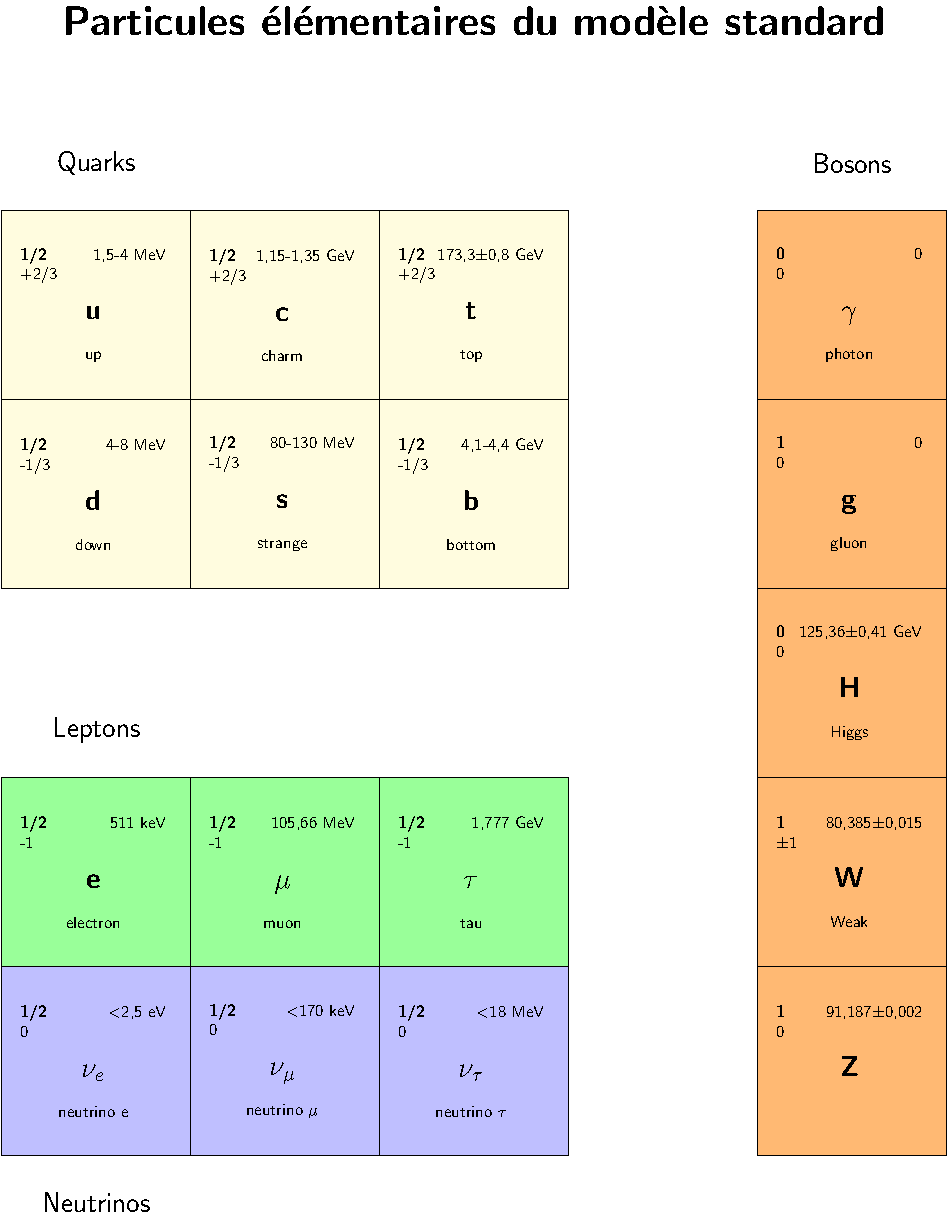
\includegraphics[width=0.9\textwidth]{table_ms.pdf}

\end{figure}

Le photon est le boson vecteur de l'interaction électromagnétique. Les bosons $W$ et $Z$ sont les bosons vecteurs de l'interaction faible. Le gluon est le boson vecteur de l'interaction forte.
L'interaction forte concerne les hadrons (particules composées de quarks).

\section{Boson de Higgs}

\subsection{Caractéristiques}

Le boson de Higgs est une particule élémentaire du modèle standard de masse $\simeq$ 125 GeV et de spin nul et découverte grâce aux expériences CMS et Atlas.
Son existence a été suggérée en 1964 afin de proposer une explication cohérente avec le modèle standard d'une masse non nulle pour les bosons de jauge $W^{\pm}$ et $Z$.

\subsection{Formation}

Il existe de nombreux processus entrainant la production de boson de Higgs. En voici des exemples envisageables ainsi que leur section efficace associée dans les conditions du LHC (Run1, $\sqrt{s} = $ 8 TeV).

\subsubsection{Fusion gluon gluon ($gg \to H$)}

La fusion gluon gluon est le mode de production du Higgs le plus important. 

La section efficace totale du processus est de 19,23 pb à $\sqrt{s} =$ 8 TeV et 43,94 pb à $\sqrt{s} =$ 13 TeV\cite{twiki_cern_higgs_cross_sections}

\begin{fmffile}{gg_H}
\begin{figure}[H]
      \centering
\begin{fmfgraph*}(140,100)
\fmfleft{i1,i2}
\fmfright{o1}

\fmflabel{$g$}{i1}
\fmflabel{$g$}{i2}
\fmflabel{$H$}{o1}

\fmf{gluon}{i1,v1}
\fmf{gluon}{i2,v2}
\fmf{dashes}{v3,o1}
\fmf{fermion,label=$q$}{v1,v2}
\fmf{fermion}{v2,v3}
\fmf{fermion}{v3,v1}
\end{fmfgraph*}
\caption{Formation d'un Higgs par fusion de gluons (avec apparition de quarks virtuels, préférentiellement lourds).  }
\end{figure}
\end{fmffile}

\subsubsection{Vector Boson Fusion (VBF, $ff \to ffH$)}

La section efficace du processus VBF est de 1,58 pb à $\sqrt{s} =$ 8 TeV et 3,75 à $\sqrt{s} =$ 13 TeV. Il s'agit du second mode de production du Higgs le plus probable.

\begin{fmffile}{VBF}
\begin{figure}[H]
      \centering
\begin{fmfgraph*}(140,100)
\fmfleft{i1,i2}
\fmfright{o1,o2,o3}

\fmflabel{$f$}{i1}
\fmflabel{$f$}{i2}
\fmflabel{$f$}{o1}
\fmflabel{$f$}{o3}
\fmflabel{$H$}{o2}
%\fmflabel{$W,Z$}{v3}

\fmf{fermion}{i1,v1,o1}
\fmf{fermion}{i2,v2,o3}
\fmf{photon,label=$W,,Z$}{v1,v3}
\fmf{photon,label=$W,,Z$}{v3,v2}
\fmf{dashes}{v3,o2}
\end{fmfgraph*}
\caption{Formation d'un Higgs par fusion de bosons $W$ ou $Z$ virtuels échangés entre deux fermions.  }
\end{figure}
\end{fmffile}

\subsubsection{Higgs Strahlung ($f\bar{f} \to WH \textrm{ ou } ZH$)}

La section efficace totale pour ce processus est $\sigma = \sigma_W + \sigma_Z$ = 0,7 $+$0,4 = 1,1 pb à $\sqrt{s} =$ 8 TeV et $\sigma =$ 2,3 à $\sqrt{s}$ = 13 TeV

\begin{fmffile}{HS}
\begin{figure}[H]
      \centering
\begin{fmfgraph*}(140,100)
\fmfleft{i1,i2}
\fmfright{o1,o2}

\fmflabel{$f$}{i1}
\fmflabel{$\bar{f}$}{i2}
\fmflabel{$W,Z$}{o1}
\fmflabel{$H$}{o2}

\fmf{fermion}{i1,v1}
\fmf{fermion}{v1,i2}
\fmf{photon,label=$W,,Z$}{v1,v2}
\fmf{photon}{v2,o1}
\fmf{dashes}{v2,o2}
\end{fmfgraph*}
\caption{La collision d'un fermion avec un antifermion peut produire un boson $W$ ou $Z$ pouvant émettre un $H$. }
\end{figure}
\end{fmffile}

\subsubsection{Top/bottom fusion (ex: $gg \to q\bar{q}H$, $q = t,b$)}


\begin{figure}[H]
\begin{subfigure}{.45\linewidth}
\begin{fmffile}{TF}
      \centering
\begin{fmfgraph*}(140,100)
\fmfleft{i1,i2}
\fmfright{o1,o2,o3}

\fmflabel{$g$}{i1}
\fmflabel{$g$}{i2}
\fmflabel{$q$}{o1}
\fmflabel{$H$}{o2}
\fmflabel{$\bar{q}$}{o3}

\fmf{gluon}{i1,v1}
\fmf{gluon}{i2,v2}

\fmf{fermion}{v1,o1}
\fmf{fermion}{o3,v2}
\fmf{fermion,label=$q$}{v2,v3}
\fmf{fermion,label=$\bar{q}$}{v3,v1}

\fmf{dashes}{v3,o2}
\end{fmfgraph*}
\caption{\\ Ici, deux gluons produisent deux paires $t\bar{t}$ ou $b\bar{b}$. Une d'entre elles fusionne et produit un $H$. Il s'agit d'un processus mineur ($\sigma = \sigma_b + \sigma_t = $ 0,20 $+$ 0,13 = 0,33 pb à 8 TeV et $\sigma = \sigma_b + \sigma_t = $ 0,6 $+$ 0,6 = 1,2 pb à 14 TeV)}
\end{fmffile}
\end{subfigure}\hfill
\begin{subfigure}{.45\linewidth}
\begin{fmffile}{TF_2}
      \centering
\begin{fmfgraph*}(140,100)
\fmfleft{i1,i2}
\fmfright{o1,o2,o3,o4}

\fmflabel{$q$}{i1}
\fmflabel{$\bar{q}$}{i2}
\fmflabel{$\over{b}$}{o1}
\fmflabel{$H$}{o2}
\fmflabel{$b$}{o3}

\fmf{fermion}{i1,v1}
\fmf{fermion}{v1,i2}
\fmf{gluon}{v1,v2}

\fmf{fermion}{v2,o3}

\fmf{fermion}{o1,v3}
\fmf{fermion}{v3,v2}
\fmf{dashes}{v3,o2}
\end{fmfgraph*}
\caption{\\ Un autre exemple de production $q\bar{q}H$ (ici $q\bar{q} \to b\bar{b}H$)}
\end{fmffile}
\end{subfigure}
\end{figure}


Ces processus sont l'objet d'une attention particulière, malgré leur faible section efficace. En effet, ils introduisent un couplage direct entre $H$ et des quarks lourds. L'intensité de ce couplage étant proportionnelle à la masse des quarks, elle est très forte dans le cas des top. Etudier ces évènements permettrait donc une mesure directe du couplage $H$ - fermion à des masses élevées. \cite{yukawa_coupling}

\subsubsection{Section efficace totale $pp \to H$}

\begin{figure}[H]
      \centering
\begin{tabular}{|r|c|} 
   \hline
   $\sqrt{s}$ (TeV) & $\sigma_{pp \to H}$ (pb) \\
    \hline
   7 &  17,5\\
\hline
   8 & 22,3 \\
\hline
   13 & 50,9  \\
\hline
   14 & 58.0 \\
  \hline
\end{tabular}
\caption{Section efficace totale pour le processus $pp \to H$ en fonction de l'énergie des faisceaux. Augmenter l'énergie augmente $\sigma_H$ de façon significative.}
\end{figure}

\subsection{Désintégration}

\begin{figure}[H]
\centering
\begin{tabular}{|l|c|r|} 
   \hline
   Type & Exemple & Ratio de branche\\
    \hline
    H $\to$ fermions & $H \to b\bar{b} $ & 57,7 \% \\
    \cline{2-3} 
        & $H \to \tau\bar{\tau} $ & 6,4 \% \\
   \cline{2-3} 
        & $H \to \mu\bar{\mu}$ & 0,02 \%\\
    \hline
  H $\to$ bosons de jauge & $H \to WW$ &21,5 \% \\
   \cline{2-3}
     & $H \to ZZ$ & 2,63 \% \\
   \cline{2-3}
      & $H \to \gamma \gamma$ & 0,23 \% \\
  \hline
\end{tabular}
\caption{Différents modes de désintégration possibles pour le Higgs, ainsi que leur probabilité respective. }
\end{figure}

\subsection{Produits de désintégration et choix de méthode d'observation}

Pour détecter la présence d'un boson de Higgs parmi un évènement il faut étudier ses produits de désintégrations et vérifier qu'ils sont compatibles avec un $H$. Il faut pour cela que les particules produites soient détéctables et que l'on puisse mesurer leurs paramètres cinématiques avec suffisamment de précision.

\begin{figure}[H]
\centering
  \caption{Résultats de l'expérience Atlas sur la détection du Higgs à travers sa désintégration par différents modes. Les signaux extraits sont comparés aux valeurs attendues selon le modèle standard. }
 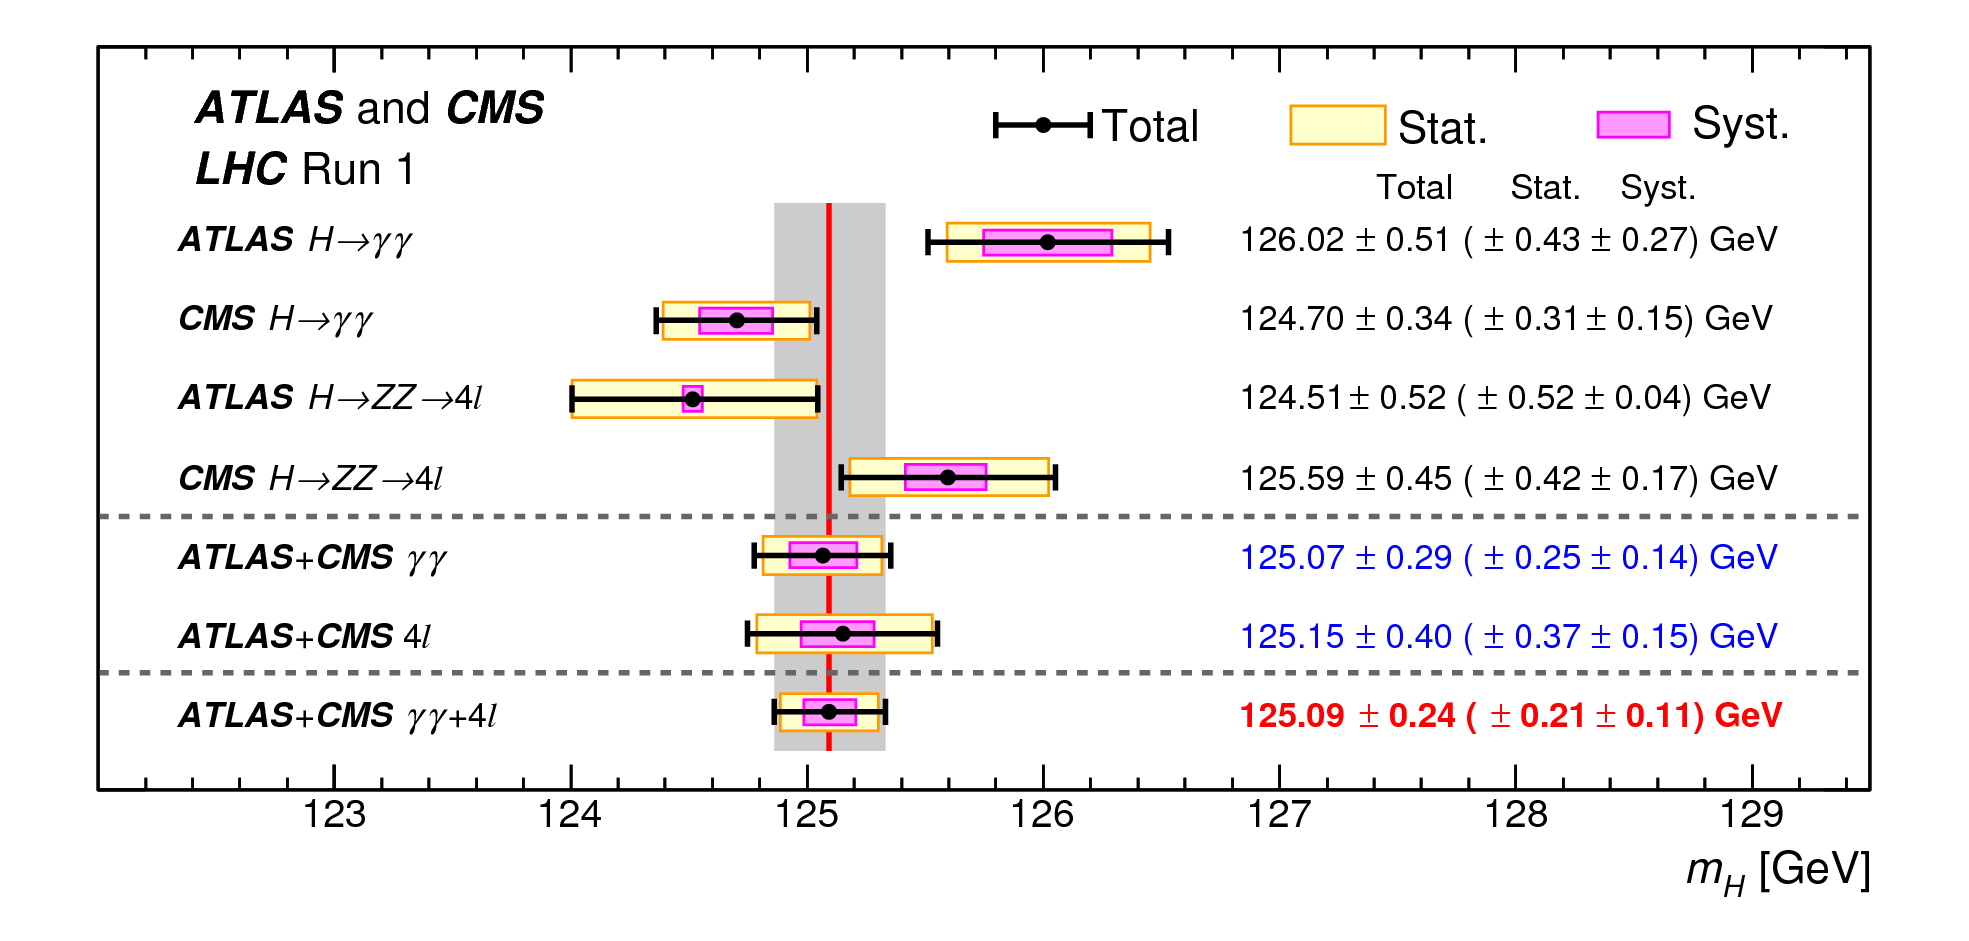
\includegraphics[width=0.9\textwidth]{../images/fig_02.png}
\end{figure}


\subsubsection{$H \to \gamma \gamma$}

La désintégration du Higgs en deux photons est une méthode d'observation privilégiée. Bien que le ratio associé à cette branche soit très faible (2 pour 1000), ce qui implique que peu de Higgs formés seront observables de cette façon, il est plus facile de détecter de tels photons avec une grande précision sur leur énergie et direction. La connaissance précise de l'impulsion de la paire de photons permet alors de remonter à la masse d'un Higgs dont ils seraient issus simplement (il s'agit de la masse invariante du système formé par la paire). Un inconvénient de ce canal est qu'il n'aurait pas permis de détecter un Higgs lourd (> 200 GeV).

\begin{figure}[H]
\centering
\begin{tabular}{|r|c|} 
   \hline
   $\sqrt{s}$ (TeV) & $\sigma_{pp \to H \to \gamma \gamma}$ (fb) \\
    \hline
   7 &  40\\
\hline
   8 & 51 \\
\hline
   13 & 117  \\
\hline
   14 & 133 \\
  \hline
\end{tabular}
\caption{Sections efficaces associées à la désintégration d'un Higgs en $\gamma \gamma$, en fonction de l'énergie du faisceau.}
\end{figure}



\subsubsection{$H \to ZZ^* \to \ell \ell \ell \ell$}

Une autre voie privilégiée est la désintégration d'un $H$ en une paire de $ZZ^*$ puis 4 leptons (4$e$, 4$\mu$ ou 2$e$2$\mu$). Bien que la section efficace totale d'un tel processus soit encore inférieure à celle de la voie $\gamma \gamma$ aux alentours de 125 GeV  (la probabilité qu'un Z se désintégrant en paire $ee$ ou $\mu \mu$ étant de 3,4 \% seulement), cette méthode est très intéressante en raison d'un excellent rapport signal/bruit et d'une précision correcte sur la masse reconstruite. De plus, dans l'hypothèse d'un Higgs lourd, les désintégrations d'un Higgs en paire de Z deviennent très probablent, et le bruit de fond très faible.

\begin{figure}[H]
\centering
\begin{tabular}{|r|c|} 
   \hline
   $\sqrt{s}$ (TeV) & $\sigma_{pp \to H \to ZZ^* \to 4\ell}$ (fb) \\
    \hline
   7 &  2,2\\
\hline
   8 & 2,7 \\
\hline
   13 & 6,2  \\
\hline
   14 & 7,0 \\
  \hline
\end{tabular}
\caption{Sections efficaces associées à la désintégration d'un Higgs en $ZZ^*$ puis 4$\ell$, en fonction de l'énergie du faisceau.}
\end{figure}

\begin{figure}[H]
\centering
  \caption{Signal et bruit de fond attendus pour différentes masses du Higgs dans le canal $4\ell$}
 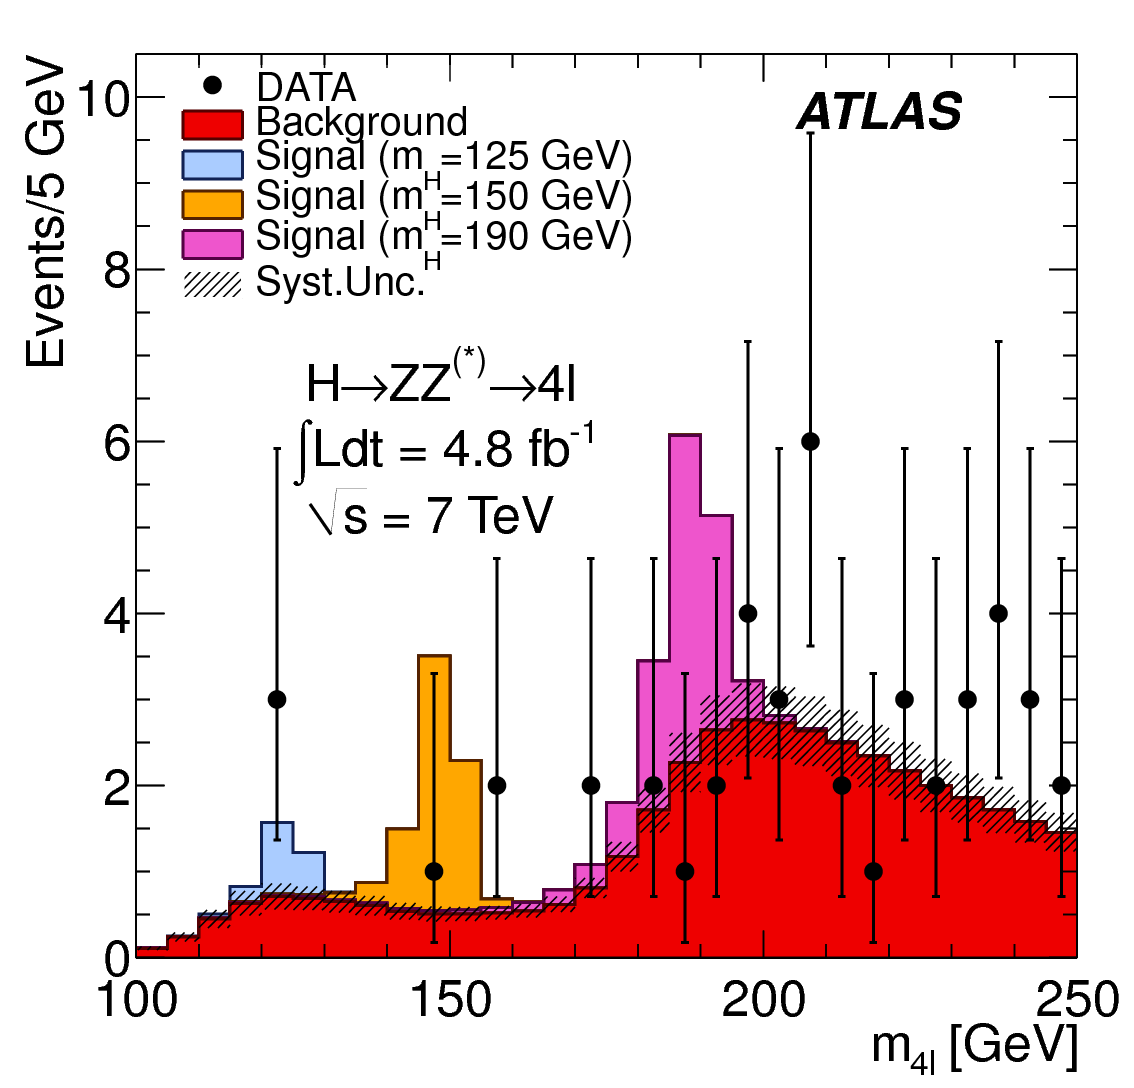
\includegraphics[width=0.9\textwidth]{../images/atlas_llll_events.png}
\end{figure}


\subsubsection{$H \to W^+W^-$}


\subsubsection{$H \to \tau^+\tau^- \to \ell\ell$, $\ell$-jet ou jet-jet}

La désintégration d'un H en paire $\tau^+ \tau^-$ offre une autre voie d'observation du Higgs. Elle pose cependant des difficultés : les particules $\tau$ ne sont pas détectables directement. Elles sont donc reconstruites à partir de leurs produits de désintégrations. Ces produits sont des hadrons (identifiables par des 'jets') dans 65 \% des cas environ et des leptons dans les 35 \% des cas restants. Cela implique une reconstruction à partir d'au moins un jet dans 90  \% des cas, qui sont soumis à un bruit de  background important. De plus, au moins un neutrino est émis (en vertu de la conservation du nombre tauonique) lors d'une désintégration d'un $\tau$, et un de plus lorsqu'il se désintègre en un autre lepton, ce qui pose problème pour la reconstruction des masses et impulsions puisque les neutrinos ne sont pas détectables.



% différentes voies, par importance et BR
% expliquer contraintes de détections et pq H->yy privilégié malgré faible BR etc..
%
%\begin{figure}[H]
%\centering
%  \caption{Statut du LHC et des faisceaux pour chaque expérience. \og Physics \fg signifie que l'expérience collecte actuellement des données qui seront utilisées dans l'analyse des résultats.  Le graphe représente l'énergie de fonctionnement du LHC ($\dfrac{\sqrt{s}}{2}$) et la luminosité des faisceaux. }
% 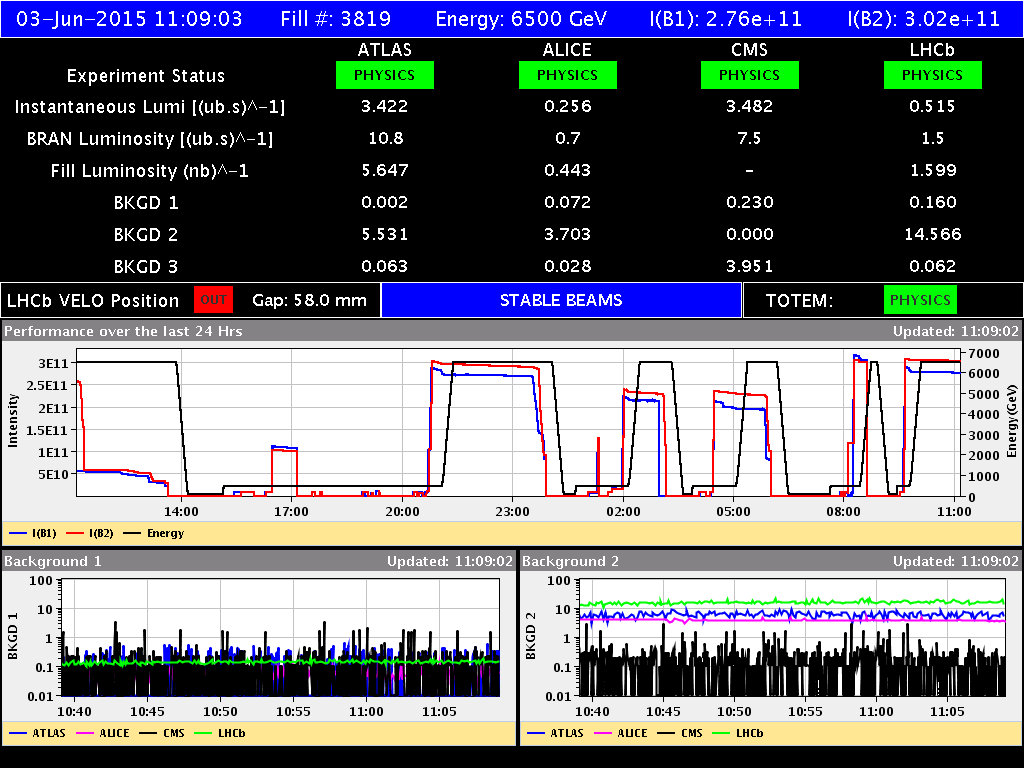
\includegraphics[width=0.9\textwidth]{../images/lhc3.png}
%\end{figure}




\section{Atlas}

\subsection{Généralités}

Atlas fait partie des 4 expériences principales situées sur le LHC (Large Hadron Collider) avec CMS, ALICE et LHCb.
Elle étudie des collisions entre protons accélérés par le LHC à des énergies de centre de masse jusqu'à 14 TeV. Son objectif est de confirmer les dernières prédictions non testées du modèle standard (Higgs) ou encore la recherche de preuves de supersymétrie et de nouvelle physique. Avec CMS, cette expérience a effectivement permis la découverte du boson de Higgs en 2013.

% à relier a ce qui a été dit précédemment sur H
\subsection{Détecteurs}

\begin{figure}[H]
\centering
  \caption{Schéma du détecteur Atlas}
\label{fig:atlas_detector}
 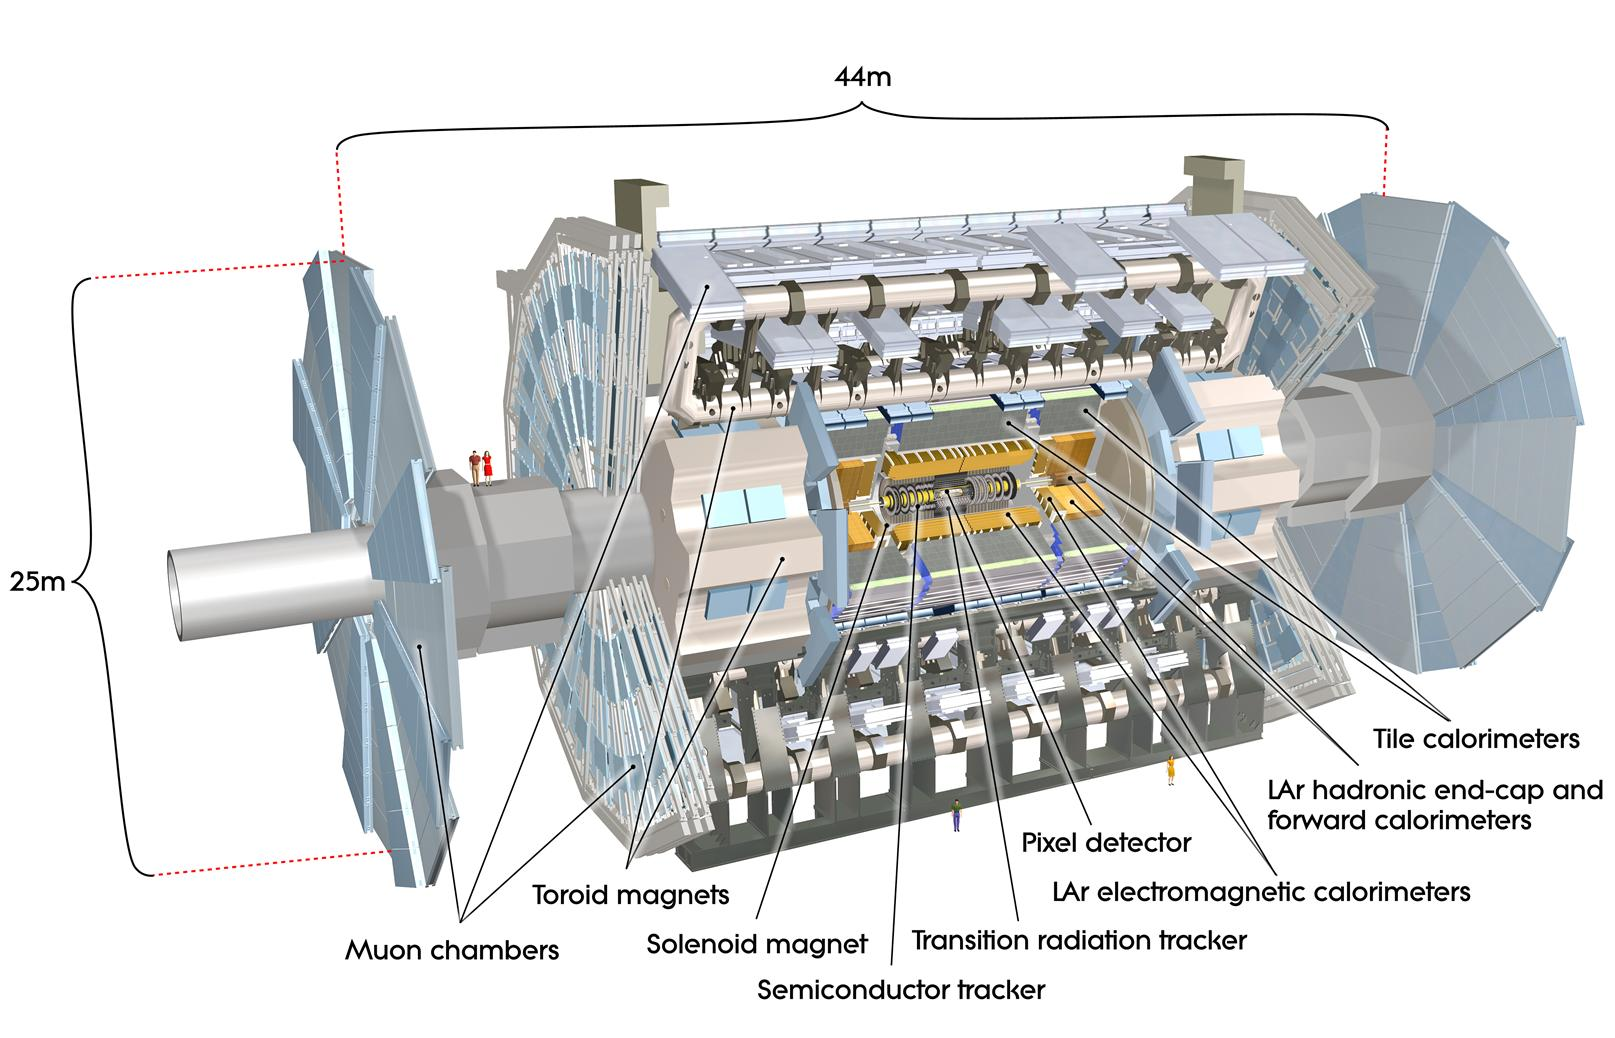
\includegraphics[width=0.9\textwidth]{../images/figures_AtlasDetectorLabelled.png}
\end{figure}

\subsubsection{Tracking, détermination de la charge et de l'impulsion}

Le détecteur intérieur (inner-detector), au plus proche des collisions, est constitué de trois sous-détecteurs : le \textbf{Pixel detector}, le \textbf{Semiconductor Detector} et le \textbf{Transition radiaton detector}. Dans les deux premiers détecteurs, le passage d'un photon ou d'une particule chargée crée des paires électrons-trous qui créent un courant mesurable sous l'influence d'un champ électrique. 
Le \textbf{Transition radiaton detector} détecte le passage des particules par ionisation d'un gaz. Il permet de plus de détecter les photons émis par rayonnement de transition lorsqu'une particule traverse successivement des milieux d'indices différents, ce qui donne une mesure directe de son facteur de Lorentz $\gamma$.

Le champ magnétique uniforme régnant dans le détecteur  intérieur  grâce au \textbf{Solenoid Magnet}courbe la trajectoire des particules chargées. En fonction des points de détection obtenus grâce à ces détecteurs il est possible de reconstruire les traces des particules et leur charge à partir du sens de la courbure ainsi que leur impulsion (à partir du rayon de courbure) :

\begin{equation} 
R_c = \dfrac{\gamma mv_{\perp}}{qB_0} = \dfrac{p_{T}}{qB_0}
\end{equation}

\subsubsection{Détermination de l'énergie et de la nature des particules}

La mesure de l'énergie des particules se fait à l'aide de deux calorimètres : un calorimètre électromagnétique (\textbf{LAr Electromagnetic Calorimeter}), et le calorimètre hadronique. Les particules susceptibles d'intéragir avec ces calorimètres génèrent des "douches". Celles-ci sont reconstruites pour remonter à l'énergie et la direction de la particule d'origine.

Les muons n'intéragissent pas avec ces détecteurs : ils sont mesurés à l'aide d'un dispositif externe (Muon spectrometer), qui repose en partie sur le tracking par rayon de courbure magnétique, à l'aide d'un champ intense mais complexe imposé par les \textbf{Toroid Magnets}.

\subsection{Performances}

La portée des résultats physiques de l'expérience repose entre autres sur les performances du détecteur. Ces performances concernent la qualité des données (résolution élevée, erreurs faibles) et de quantité (peu d'évènements "perdus"). Elles peuvent être évaluées expérimentalement ou anticipées grâce à des modèles. Ici, on utilise des données issues de simulation Monte-Carlo afin d'estimer quantitativement les performances des détecteurs qui sont importantes pour l'étude des évènements $H \to \gamma \gamma$.

\subsubsection{Résolution en énergie du calorimètre EM}

Plusieurs facteurs limitent la résolution en énergie du calorimètre. Celle-ci peut être évaluée de la façon suivante :

\begin{equation}
\dfrac{\sigma_E}{E} \simeq \dfrac{a}{\sqrt{E}} \oplus \dfrac{b}{E} \oplus c
\end{equation}

Le terme $\propto a$ représente l'erreur d'origine statistique, $b$ le bruit électronique et $c$ les erreurs constantes de non-linéarité/calibration..

Aux énergies qui nous intéressent (> 10 GeV), le bruit électronique est négligeable ($b \sim$ 100 MeV) et la résolution prend une forme :

\begin{equation}
\dfrac{\sigma_E}{E} \sim \dfrac{a}{\sqrt{E}} \oplus c
\end{equation}

A l'aide des simulations Monte-Carlo, on estime la résolution en énergie en fonction de l'énergie des photons mesurés, afin de vérifier si ce comportement est bien reproduit. Pour cela, on compare les données vraies aux données telles qu'elles devraient être reconstruites par le détecteur. (figures \ref{fig:resolution_energie_photons_tab}, \ref{fig:resolution_energie_photons} et \ref{fig:resolution_energie_photons2}).

\begin{figure}[H]
\centering
\begin{tabular}{|l|c|r|r|} 
   \hline
   Photons convertis inclus &$\eta$ & $a$(\% $\cdot$ GeV${ }^{1/2}$) & $c (\%)$ \\
    \hline
   Oui & tous & 18  $\pm$ 1  &0,6  $\pm$ 0,1  \\
  \hline
   Non & tous & 13  $\pm$ 1  &0,8  $\pm$ 0,1  \\
  \hline
   Oui &$|\eta| < $ 1 & 10  $\pm$ 1  &0,9  $\pm$ 0,1  \\
\hline
   Oui & $|\eta| >$ 1,5 & 13  $\pm$ 2  &1,8  $\pm$ 0,2  \\
\hline
\end{tabular}
\caption{ Pour plusieurs bandes d'énergie, on calcule l'écart entre les données vraies et reconstruites à partir d'une simulation. On obtient les paramètres $a$ et $c$ après fit de $E \mapsto \sigma_E(E)$.  }
\label{fig:resolution_energie_photons_tab} 
\end{figure}

\begin{figure}[H]
\begin{subfigure}[b]{.5\linewidth}
\centering
  \caption{Photons 'tight' }
\label{fig:resolution_energie_photons} 
 \resizebox{1.1\linewidth}{!}{\begin{tikzpicture}
\pgfdeclareplotmark{cross} {
\pgfpathmoveto{\pgfpoint{-0.3\pgfplotmarksize}{\pgfplotmarksize}}
\pgfpathlineto{\pgfpoint{+0.3\pgfplotmarksize}{\pgfplotmarksize}}
\pgfpathlineto{\pgfpoint{+0.3\pgfplotmarksize}{0.3\pgfplotmarksize}}
\pgfpathlineto{\pgfpoint{+1\pgfplotmarksize}{0.3\pgfplotmarksize}}
\pgfpathlineto{\pgfpoint{+1\pgfplotmarksize}{-0.3\pgfplotmarksize}}
\pgfpathlineto{\pgfpoint{+0.3\pgfplotmarksize}{-0.3\pgfplotmarksize}}
\pgfpathlineto{\pgfpoint{+0.3\pgfplotmarksize}{-1.\pgfplotmarksize}}
\pgfpathlineto{\pgfpoint{-0.3\pgfplotmarksize}{-1.\pgfplotmarksize}}
\pgfpathlineto{\pgfpoint{-0.3\pgfplotmarksize}{-0.3\pgfplotmarksize}}
\pgfpathlineto{\pgfpoint{-1.\pgfplotmarksize}{-0.3\pgfplotmarksize}}
\pgfpathlineto{\pgfpoint{-1.\pgfplotmarksize}{0.3\pgfplotmarksize}}
\pgfpathlineto{\pgfpoint{-0.3\pgfplotmarksize}{0.3\pgfplotmarksize}}
\pgfpathclose
\pgfusepathqstroke
}
\pgfdeclareplotmark{cross*} {
\pgfpathmoveto{\pgfpoint{-0.3\pgfplotmarksize}{\pgfplotmarksize}}
\pgfpathlineto{\pgfpoint{+0.3\pgfplotmarksize}{\pgfplotmarksize}}
\pgfpathlineto{\pgfpoint{+0.3\pgfplotmarksize}{0.3\pgfplotmarksize}}
\pgfpathlineto{\pgfpoint{+1\pgfplotmarksize}{0.3\pgfplotmarksize}}
\pgfpathlineto{\pgfpoint{+1\pgfplotmarksize}{-0.3\pgfplotmarksize}}
\pgfpathlineto{\pgfpoint{+0.3\pgfplotmarksize}{-0.3\pgfplotmarksize}}
\pgfpathlineto{\pgfpoint{+0.3\pgfplotmarksize}{-1.\pgfplotmarksize}}
\pgfpathlineto{\pgfpoint{-0.3\pgfplotmarksize}{-1.\pgfplotmarksize}}
\pgfpathlineto{\pgfpoint{-0.3\pgfplotmarksize}{-0.3\pgfplotmarksize}}
\pgfpathlineto{\pgfpoint{-1.\pgfplotmarksize}{-0.3\pgfplotmarksize}}
\pgfpathlineto{\pgfpoint{-1.\pgfplotmarksize}{0.3\pgfplotmarksize}}
\pgfpathlineto{\pgfpoint{-0.3\pgfplotmarksize}{0.3\pgfplotmarksize}}
\pgfpathclose
\pgfusepathqfillstroke
}
\pgfdeclareplotmark{newstar} {
\pgfpathmoveto{\pgfqpoint{0pt}{\pgfplotmarksize}}
\pgfpathlineto{\pgfqpointpolar{44}{0.5\pgfplotmarksize}}
\pgfpathlineto{\pgfqpointpolar{18}{\pgfplotmarksize}}
\pgfpathlineto{\pgfqpointpolar{-20}{0.5\pgfplotmarksize}}
\pgfpathlineto{\pgfqpointpolar{-54}{\pgfplotmarksize}}
\pgfpathlineto{\pgfqpointpolar{-90}{0.5\pgfplotmarksize}}
\pgfpathlineto{\pgfqpointpolar{234}{\pgfplotmarksize}}
\pgfpathlineto{\pgfqpointpolar{198}{0.5\pgfplotmarksize}}
\pgfpathlineto{\pgfqpointpolar{162}{\pgfplotmarksize}}
\pgfpathlineto{\pgfqpointpolar{134}{0.5\pgfplotmarksize}}
\pgfpathclose
\pgfusepathqstroke
}
\pgfdeclareplotmark{newstar*} {
\pgfpathmoveto{\pgfqpoint{0pt}{\pgfplotmarksize}}
\pgfpathlineto{\pgfqpointpolar{44}{0.5\pgfplotmarksize}}
\pgfpathlineto{\pgfqpointpolar{18}{\pgfplotmarksize}}
\pgfpathlineto{\pgfqpointpolar{-20}{0.5\pgfplotmarksize}}
\pgfpathlineto{\pgfqpointpolar{-54}{\pgfplotmarksize}}
\pgfpathlineto{\pgfqpointpolar{-90}{0.5\pgfplotmarksize}}
\pgfpathlineto{\pgfqpointpolar{234}{\pgfplotmarksize}}
\pgfpathlineto{\pgfqpointpolar{198}{0.5\pgfplotmarksize}}
\pgfpathlineto{\pgfqpointpolar{162}{\pgfplotmarksize}}
\pgfpathlineto{\pgfqpointpolar{134}{0.5\pgfplotmarksize}}
\pgfpathclose
\pgfusepathqfillstroke
}
\definecolor{c}{rgb}{1,1,1};
\draw [color=c, fill=c] (0,0) rectangle (20,13.6207);
\draw [color=c, fill=c] (2,1.36207) rectangle (18,12.2586);
\definecolor{c}{rgb}{0,0,0};
\draw [c,line width=0.9] (2,1.36207) -- (2,12.2586) -- (18,12.2586) -- (18,1.36207) -- (2,1.36207);
\definecolor{c}{rgb}{1,1,1};
\draw [color=c, fill=c] (2,1.36207) rectangle (18,12.2586);
\definecolor{c}{rgb}{0,0,0};
\draw [c,line width=0.9] (2,1.36207) -- (2,12.2586) -- (18,12.2586) -- (18,1.36207) -- (2,1.36207);
\draw [c,line width=0.9] (2,1.36207) -- (18,1.36207);
\draw [anchor= east] (18,0.599311) node[scale=1.08496, color=c, rotate=0]{$E\mbox{ (GeV) }$};
\draw [c,line width=0.9] (2.45455,1.68897) -- (2.45455,1.36207);
\draw [c,line width=0.9] (2.93939,1.52552) -- (2.93939,1.36207);
\draw [c,line width=0.9] (3.42424,1.52552) -- (3.42424,1.36207);
\draw [c,line width=0.9] (3.90909,1.52552) -- (3.90909,1.36207);
\draw [c,line width=0.9] (4.39394,1.52552) -- (4.39394,1.36207);
\draw [c,line width=0.9] (4.87879,1.68897) -- (4.87879,1.36207);
\draw [c,line width=0.9] (5.36364,1.52552) -- (5.36364,1.36207);
\draw [c,line width=0.9] (5.84848,1.52552) -- (5.84848,1.36207);
\draw [c,line width=0.9] (6.33333,1.52552) -- (6.33333,1.36207);
\draw [c,line width=0.9] (6.81818,1.52552) -- (6.81818,1.36207);
\draw [c,line width=0.9] (7.30303,1.68897) -- (7.30303,1.36207);
\draw [c,line width=0.9] (7.78788,1.52552) -- (7.78788,1.36207);
\draw [c,line width=0.9] (8.27273,1.52552) -- (8.27273,1.36207);
\draw [c,line width=0.9] (8.75758,1.52552) -- (8.75758,1.36207);
\draw [c,line width=0.9] (9.24242,1.52552) -- (9.24242,1.36207);
\draw [c,line width=0.9] (9.72727,1.68897) -- (9.72727,1.36207);
\draw [c,line width=0.9] (10.2121,1.52552) -- (10.2121,1.36207);
\draw [c,line width=0.9] (10.697,1.52552) -- (10.697,1.36207);
\draw [c,line width=0.9] (11.1818,1.52552) -- (11.1818,1.36207);
\draw [c,line width=0.9] (11.6667,1.52552) -- (11.6667,1.36207);
\draw [c,line width=0.9] (12.1515,1.68897) -- (12.1515,1.36207);
\draw [c,line width=0.9] (12.6364,1.52552) -- (12.6364,1.36207);
\draw [c,line width=0.9] (13.1212,1.52552) -- (13.1212,1.36207);
\draw [c,line width=0.9] (13.6061,1.52552) -- (13.6061,1.36207);
\draw [c,line width=0.9] (14.0909,1.52552) -- (14.0909,1.36207);
\draw [c,line width=0.9] (14.5758,1.68897) -- (14.5758,1.36207);
\draw [c,line width=0.9] (15.0606,1.52552) -- (15.0606,1.36207);
\draw [c,line width=0.9] (15.5455,1.52552) -- (15.5455,1.36207);
\draw [c,line width=0.9] (16.0303,1.52552) -- (16.0303,1.36207);
\draw [c,line width=0.9] (16.5152,1.52552) -- (16.5152,1.36207);
\draw [c,line width=0.9] (17,1.68897) -- (17,1.36207);
\draw [c,line width=0.9] (2.45455,1.68897) -- (2.45455,1.36207);
\draw [c,line width=0.9] (17,1.68897) -- (17,1.36207);
\draw [c,line width=0.9] (17.4848,1.52552) -- (17.4848,1.36207);
\draw [c,line width=0.9] (17.9697,1.52552) -- (17.9697,1.36207);
\draw [anchor=base] (2.45455,0.912586) node[scale=1.08496, color=c, rotate=0]{100};
\draw [anchor=base] (4.87879,0.912586) node[scale=1.08496, color=c, rotate=0]{200};
\draw [anchor=base] (7.30303,0.912586) node[scale=1.08496, color=c, rotate=0]{300};
\draw [anchor=base] (9.72727,0.912586) node[scale=1.08496, color=c, rotate=0]{400};
\draw [anchor=base] (12.1515,0.912586) node[scale=1.08496, color=c, rotate=0]{500};
\draw [anchor=base] (14.5758,0.912586) node[scale=1.08496, color=c, rotate=0]{600};
\draw [anchor=base] (17,0.912586) node[scale=1.08496, color=c, rotate=0]{700};
\draw [c,line width=0.9] (2,1.36207) -- (2,12.2586);
\draw [anchor= east] (0.88,12.2586) node[scale=1.08496, color=c, rotate=90]{$\sigma_{E} / E \mbox{ \% }$};
\draw [c,line width=0.9] (2.48,2.07436) -- (2,2.07436);
\draw [c,line width=0.9] (2.24,2.59944) -- (2,2.59944);
\draw [c,line width=0.9] (2.24,3.12451) -- (2,3.12451);
\draw [c,line width=0.9] (2.24,3.64959) -- (2,3.64959);
\draw [c,line width=0.9] (2.48,4.17467) -- (2,4.17467);
\draw [c,line width=0.9] (2.24,4.69974) -- (2,4.69974);
\draw [c,line width=0.9] (2.24,5.22482) -- (2,5.22482);
\draw [c,line width=0.9] (2.24,5.74989) -- (2,5.74989);
\draw [c,line width=0.9] (2.48,6.27497) -- (2,6.27497);
\draw [c,line width=0.9] (2.24,6.80004) -- (2,6.80004);
\draw [c,line width=0.9] (2.24,7.32512) -- (2,7.32512);
\draw [c,line width=0.9] (2.24,7.8502) -- (2,7.8502);
\draw [c,line width=0.9] (2.48,8.37527) -- (2,8.37527);
\draw [c,line width=0.9] (2.24,8.90035) -- (2,8.90035);
\draw [c,line width=0.9] (2.24,9.42542) -- (2,9.42542);
\draw [c,line width=0.9] (2.24,9.9505) -- (2,9.9505);
\draw [c,line width=0.9] (2.48,10.4756) -- (2,10.4756);
\draw [c,line width=0.9] (2.48,2.07436) -- (2,2.07436);
\draw [c,line width=0.9] (2.24,1.54929) -- (2,1.54929);
\draw [c,line width=0.9] (2.48,10.4756) -- (2,10.4756);
\draw [c,line width=0.9] (2.24,11.0007) -- (2,11.0007);
\draw [c,line width=0.9] (2.24,11.5257) -- (2,11.5257);
\draw [c,line width=0.9] (2.24,12.0508) -- (2,12.0508);
\draw [anchor= east] (1.9,2.07436) node[scale=1.08496, color=c, rotate=0]{1.2};
\draw [anchor= east] (1.9,4.17467) node[scale=1.08496, color=c, rotate=0]{1.4};
\draw [anchor= east] (1.9,6.27497) node[scale=1.08496, color=c, rotate=0]{1.6};
\draw [anchor= east] (1.9,8.37527) node[scale=1.08496, color=c, rotate=0]{1.8};
\draw [anchor= east] (1.9,10.4756) node[scale=1.08496, color=c, rotate=0]{2};
\foreach \P in
 {(3.66667,11.1817),(4.33333,10.4626),(5,9.6506),(5.66667,8.13577),(6.33333,7.02294),(7,6.86235),(7.66667,6.36704),(8.33333,6.01511),(9,5.44942),(9.66667,5.42913),(10.3333,5.36333),(11,5.35065),(11.6667,4.73358),(12.3333,4.12402),(13,3.67607),(13.666
7,4.32407),(14.3333,3.49205),(15,4.02828),(15.6667,3.99242),(16.3333,2.7789)}{\draw[mark options={color=c,fill=c},mark size=2.402402pt,mark=*,mark size=1pt] plot coordinates {\P};}
\definecolor{c}{rgb}{1,0,0};
\draw [c,line width=1.8] (3.04,12.2586) -- (3.2,12.2496) -- (3.36,11.8591) -- (3.52,11.4958) -- (3.68,11.1566) -- (3.84,10.839) -- (4,10.5409) -- (4.16,10.2602) -- (4.32,9.99539) -- (4.48,9.74498) -- (4.64,9.50774) -- (4.8,9.28253) -- (4.96,9.06837)
 -- (5.12,8.8644) -- (5.28,8.66982) -- (5.44,8.48394) -- (5.6,8.30613) -- (5.76,8.13582) -- (5.92,7.97249) -- (6.08,7.81569) -- (6.24,7.66499) -- (6.4,7.52001) -- (6.56,7.38039) -- (6.72,7.2458) -- (6.88,7.11596) -- (7.04,6.99059) -- (7.2,6.86944) --
 (7.36,6.75229) -- (7.52,6.6389) -- (7.68,6.52909) -- (7.84,6.42267) -- (8,6.31948) -- (8.16,6.21934) -- (8.32,6.12212) -- (8.48,6.02768) -- (8.64,5.93588) -- (8.8,5.8466) -- (8.96,5.75973) -- (9.12,5.67517) -- (9.28,5.59281) -- (9.44,5.51256) --
 (9.6,5.43433) -- (9.76,5.35804) -- (9.92,5.28361) -- (10.08,5.21096) -- (10.24,5.14003) -- (10.4,5.07074) -- (10.56,5.00304) -- (10.72,4.93687) -- (10.88,4.87216);
\draw [c,line width=1.8] (10.88,4.87216) -- (11.04,4.80888) -- (11.2,4.74695) -- (11.36,4.68634) -- (11.52,4.62701) -- (11.68,4.5689) -- (11.84,4.51197) -- (12,4.45619) -- (12.16,4.40152) -- (12.32,4.34792) -- (12.48,4.29535) -- (12.64,4.24379) --
 (12.8,4.1932) -- (12.96,4.14355) -- (13.12,4.09482) -- (13.28,4.04697) -- (13.44,3.99998) -- (13.6,3.95382) -- (13.76,3.90848) -- (13.92,3.86391) -- (14.08,3.82012) -- (14.24,3.77706) -- (14.4,3.73473) -- (14.56,3.69309) -- (14.72,3.65214) --
 (14.88,3.61185) -- (15.04,3.57221) -- (15.2,3.5332) -- (15.36,3.4948) -- (15.52,3.45699) -- (15.68,3.41977) -- (15.84,3.38311) -- (16,3.34701) -- (16.16,3.31144) -- (16.32,3.2764) -- (16.48,3.24187) -- (16.64,3.20785) -- (16.8,3.17431) --
 (16.96,3.14124) -- (17.12,3.10865) -- (17.28,3.0765) -- (17.44,3.0448) -- (17.6,3.01354) -- (17.76,2.9827) -- (17.92,2.95227);
\definecolor{c}{rgb}{0,0,0};
\draw [c,line width=0] (3.66667,11.1817) -- (3.33333,11.1817);
\draw [c,line width=0] (3.33333,11.1242) -- (3.33333,11.2391);
\draw [c,line width=0] (3.66667,11.1817) -- (4,11.1817);
\draw [c,line width=0] (4,11.1242) -- (4,11.2391);
\draw [c,line width=0] (3.66667,11.1817) -- (3.66667,11.3506);
\draw [c,line width=0] (3.6092,11.3506) -- (3.72414,11.3506);
\draw [c,line width=0] (3.66667,11.1817) -- (3.66667,11.0128);
\draw [c,line width=0] (3.6092,11.0128) -- (3.72414,11.0128);
\draw [c,line width=0] (4.33333,10.4626) -- (4,10.4626);
\draw [c,line width=0] (4,10.4052) -- (4,10.5201);
\draw [c,line width=0] (4.33333,10.4626) -- (4.66667,10.4626);
\draw [c,line width=0] (4.66667,10.4052) -- (4.66667,10.5201);
\draw [c,line width=0] (4.33333,10.4626) -- (4.33333,10.6267);
\draw [c,line width=0] (4.27586,10.6267) -- (4.3908,10.6267);
\draw [c,line width=0] (4.33333,10.4626) -- (4.33333,10.2986);
\draw [c,line width=0] (4.27586,10.2986) -- (4.3908,10.2986);
\draw [c,line width=0] (5,9.6506) -- (4.66667,9.6506);
\draw [c,line width=0] (4.66667,9.59313) -- (4.66667,9.70807);
\draw [c,line width=0] (5,9.6506) -- (5.33333,9.6506);
\draw [c,line width=0] (5.33333,9.59313) -- (5.33333,9.70807);
\draw [c,line width=0] (5,9.6506) -- (5,9.81286);
\draw [c,line width=0] (4.94253,9.81286) -- (5.05747,9.81286);
\draw [c,line width=0] (5,9.6506) -- (5,9.48834);
\draw [c,line width=0] (4.94253,9.48834) -- (5.05747,9.48834);
\draw [c,line width=0] (5.66667,8.13577) -- (5.33333,8.13577);
\draw [c,line width=0] (5.33333,8.0783) -- (5.33333,8.19324);
\draw [c,line width=0] (5.66667,8.13577) -- (6,8.13577);
\draw [c,line width=0] (6,8.0783) -- (6,8.19324);
\draw [c,line width=0] (5.66667,8.13577) -- (5.66667,8.29207);
\draw [c,line width=0] (5.6092,8.29207) -- (5.72414,8.29207);
\draw [c,line width=0] (5.66667,8.13577) -- (5.66667,7.97946);
\draw [c,line width=0] (5.6092,7.97946) -- (5.72414,7.97946);
\draw [c,line width=0] (6.33333,7.02294) -- (6,7.02294);
\draw [c,line width=0] (6,6.96547) -- (6,7.08041);
\draw [c,line width=0] (6.33333,7.02294) -- (6.66667,7.02294);
\draw [c,line width=0] (6.66667,6.96547) -- (6.66667,7.08041);
\draw [c,line width=0] (6.33333,7.02294) -- (6.33333,7.17745);
\draw [c,line width=0] (6.27586,7.17745) -- (6.3908,7.17745);
\draw [c,line width=0] (6.33333,7.02294) -- (6.33333,6.86843);
\draw [c,line width=0] (6.27586,6.86843) -- (6.3908,6.86843);
\draw [c,line width=0] (7,6.86235) -- (6.66667,6.86235);
\draw [c,line width=0] (6.66667,6.80488) -- (6.66667,6.91982);
\draw [c,line width=0] (7,6.86235) -- (7.33333,6.86235);
\draw [c,line width=0] (7.33333,6.80488) -- (7.33333,6.91982);
\draw [c,line width=0] (7,6.86235) -- (7,7.02414);
\draw [c,line width=0] (6.94253,7.02414) -- (7.05747,7.02414);
\draw [c,line width=0] (7,6.86235) -- (7,6.70055);
\draw [c,line width=0] (6.94253,6.70055) -- (7.05747,6.70055);
\draw [c,line width=0] (7.66667,6.36704) -- (7.33333,6.36704);
\draw [c,line width=0] (7.33333,6.30957) -- (7.33333,6.42451);
\draw [c,line width=0] (7.66667,6.36704) -- (8,6.36704);
\draw [c,line width=0] (8,6.30957) -- (8,6.42451);
\draw [c,line width=0] (7.66667,6.36704) -- (7.66667,6.53414);
\draw [c,line width=0] (7.6092,6.53414) -- (7.72414,6.53414);
\draw [c,line width=0] (7.66667,6.36704) -- (7.66667,6.19994);
\draw [c,line width=0] (7.6092,6.19994) -- (7.72414,6.19994);
\draw [c,line width=0] (8.33333,6.01511) -- (8,6.01511);
\draw [c,line width=0] (8,5.95764) -- (8,6.07259);
\draw [c,line width=0] (8.33333,6.01511) -- (8.66667,6.01511);
\draw [c,line width=0] (8.66667,5.95764) -- (8.66667,6.07259);
\draw [c,line width=0] (8.33333,6.01511) -- (8.33333,6.19181);
\draw [c,line width=0] (8.27586,6.19181) -- (8.3908,6.19181);
\draw [c,line width=0] (8.33333,6.01511) -- (8.33333,5.83842);
\draw [c,line width=0] (8.27586,5.83842) -- (8.3908,5.83842);
\draw [c,line width=0] (9,5.44942) -- (8.66667,5.44942);
\draw [c,line width=0] (8.66667,5.39194) -- (8.66667,5.50689);
\draw [c,line width=0] (9,5.44942) -- (9.33333,5.44942);
\draw [c,line width=0] (9.33333,5.39194) -- (9.33333,5.50689);
\draw [c,line width=0] (9,5.44942) -- (9,5.63012);
\draw [c,line width=0] (8.94253,5.63012) -- (9.05747,5.63012);
\draw [c,line width=0] (9,5.44942) -- (9,5.26871);
\draw [c,line width=0] (8.94253,5.26871) -- (9.05747,5.26871);
\draw [c,line width=0] (9.66667,5.42913) -- (9.33333,5.42913);
\draw [c,line width=0] (9.33333,5.37166) -- (9.33333,5.4866);
\draw [c,line width=0] (9.66667,5.42913) -- (10,5.42913);
\draw [c,line width=0] (10,5.37166) -- (10,5.4866);
\draw [c,line width=0] (9.66667,5.42913) -- (9.66667,5.62535);
\draw [c,line width=0] (9.6092,5.62535) -- (9.72414,5.62535);
\draw [c,line width=0] (9.66667,5.42913) -- (9.66667,5.23291);
\draw [c,line width=0] (9.6092,5.23291) -- (9.72414,5.23291);
\draw [c,line width=0] (10.3333,5.36333) -- (10,5.36333);
\draw [c,line width=0] (10,5.30586) -- (10,5.4208);
\draw [c,line width=0] (10.3333,5.36333) -- (10.6667,5.36333);
\draw [c,line width=0] (10.6667,5.30586) -- (10.6667,5.4208);
\draw [c,line width=0] (10.3333,5.36333) -- (10.3333,5.57898);
\draw [c,line width=0] (10.2759,5.57898) -- (10.3908,5.57898);
\draw [c,line width=0] (10.3333,5.36333) -- (10.3333,5.14769);
\draw [c,line width=0] (10.2759,5.14769) -- (10.3908,5.14769);
\draw [c,line width=0] (11,5.35065) -- (10.6667,5.35065);
\draw [c,line width=0] (10.6667,5.29318) -- (10.6667,5.40812);
\draw [c,line width=0] (11,5.35065) -- (11.3333,5.35065);
\draw [c,line width=0] (11.3333,5.29318) -- (11.3333,5.40812);
\draw [c,line width=0] (11,5.35065) -- (11,5.5841);
\draw [c,line width=0] (10.9425,5.5841) -- (11.0575,5.5841);
\draw [c,line width=0] (11,5.35065) -- (11,5.1172);
\draw [c,line width=0] (10.9425,5.1172) -- (11.0575,5.1172);
\draw [c,line width=0] (11.6667,4.73358) -- (11.3333,4.73358);
\draw [c,line width=0] (11.3333,4.67611) -- (11.3333,4.79105);
\draw [c,line width=0] (11.6667,4.73358) -- (12,4.73358);
\draw [c,line width=0] (12,4.67611) -- (12,4.79105);
\draw [c,line width=0] (11.6667,4.73358) -- (11.6667,4.98286);
\draw [c,line width=0] (11.6092,4.98286) -- (11.7241,4.98286);
\draw [c,line width=0] (11.6667,4.73358) -- (11.6667,4.48431);
\draw [c,line width=0] (11.6092,4.48431) -- (11.7241,4.48431);
\draw [c,line width=0] (12.3333,4.12402) -- (12,4.12402);
\draw [c,line width=0] (12,4.06655) -- (12,4.18149);
\draw [c,line width=0] (12.3333,4.12402) -- (12.6667,4.12402);
\draw [c,line width=0] (12.6667,4.06655) -- (12.6667,4.18149);
\draw [c,line width=0] (12.3333,4.12402) -- (12.3333,4.38789);
\draw [c,line width=0] (12.2759,4.38789) -- (12.3908,4.38789);
\draw [c,line width=0] (12.3333,4.12402) -- (12.3333,3.86015);
\draw [c,line width=0] (12.2759,3.86015) -- (12.3908,3.86015);
\draw [c,line width=0] (13,3.67607) -- (12.6667,3.67607);
\draw [c,line width=0] (12.6667,3.6186) -- (12.6667,3.73354);
\draw [c,line width=0] (13,3.67607) -- (13.3333,3.67607);
\draw [c,line width=0] (13.3333,3.6186) -- (13.3333,3.73354);
\draw [c,line width=0] (13,3.67607) -- (13,3.96197);
\draw [c,line width=0] (12.9425,3.96197) -- (13.0575,3.96197);
\draw [c,line width=0] (13,3.67607) -- (13,3.39016);
\draw [c,line width=0] (12.9425,3.39016) -- (13.0575,3.39016);
\draw [c,line width=0] (13.6667,4.32407) -- (13.3333,4.32407);
\draw [c,line width=0] (13.3333,4.2666) -- (13.3333,4.38154);
\draw [c,line width=0] (13.6667,4.32407) -- (14,4.32407);
\draw [c,line width=0] (14,4.2666) -- (14,4.38154);
\draw [c,line width=0] (13.6667,4.32407) -- (13.6667,4.65936);
\draw [c,line width=0] (13.6092,4.65936) -- (13.7241,4.65936);
\draw [c,line width=0] (13.6667,4.32407) -- (13.6667,3.98878);
\draw [c,line width=0] (13.6092,3.98878) -- (13.7241,3.98878);
\draw [c,line width=0] (14.3333,3.49205) -- (14,3.49205);
\draw [c,line width=0] (14,3.43458) -- (14,3.54952);
\draw [c,line width=0] (14.3333,3.49205) -- (14.6667,3.49205);
\draw [c,line width=0] (14.6667,3.43458) -- (14.6667,3.54952);
\draw [c,line width=0] (14.3333,3.49205) -- (14.3333,3.85058);
\draw [c,line width=0] (14.2759,3.85058) -- (14.3908,3.85058);
\draw [c,line width=0] (14.3333,3.49205) -- (14.3333,3.13352);
\draw [c,line width=0] (14.2759,3.13352) -- (14.3908,3.13352);
\draw [c,line width=0] (15,4.02828) -- (14.6667,4.02828);
\draw [c,line width=0] (14.6667,3.97081) -- (14.6667,4.08575);
\draw [c,line width=0] (15,4.02828) -- (15.3333,4.02828);
\draw [c,line width=0] (15.3333,3.97081) -- (15.3333,4.08575);
\draw [c,line width=0] (15,4.02828) -- (15,4.43624);
\draw [c,line width=0] (14.9425,4.43624) -- (15.0575,4.43624);
\draw [c,line width=0] (15,4.02828) -- (15,3.62032);
\draw [c,line width=0] (14.9425,3.62032) -- (15.0575,3.62032);
\draw [c,line width=0] (15.6667,3.99242) -- (15.3333,3.99242);
\draw [c,line width=0] (15.3333,3.93495) -- (15.3333,4.0499);
\draw [c,line width=0] (15.6667,3.99242) -- (16,3.99242);
\draw [c,line width=0] (16,3.93495) -- (16,4.0499);
\draw [c,line width=0] (15.6667,3.99242) -- (15.6667,4.45577);
\draw [c,line width=0] (15.6092,4.45577) -- (15.7241,4.45577);
\draw [c,line width=0] (15.6667,3.99242) -- (15.6667,3.52908);
\draw [c,line width=0] (15.6092,3.52908) -- (15.7241,3.52908);
\draw [c,line width=0] (16.3333,2.7789) -- (16,2.7789);
\draw [c,line width=0] (16,2.72142) -- (16,2.83637);
\draw [c,line width=0] (16.3333,2.7789) -- (16.6667,2.7789);
\draw [c,line width=0] (16.6667,2.72142) -- (16.6667,2.83637);
\draw [c,line width=0] (16.3333,2.7789) -- (16.3333,3.28768);
\draw [c,line width=0] (16.2759,3.28768) -- (16.3908,3.28768);
\draw [c,line width=0] (16.3333,2.7789) -- (16.3333,2.27012);
\draw [c,line width=0] (16.2759,2.27012) -- (16.3908,2.27012);
\draw (10,13.1388) node[scale=1.5317, color=c, rotate=0]{$\mbox{Resolution en energie}$};
\end{tikzpicture}
}
\end{subfigure}
\begin{subfigure}[b]{.5\linewidth}
\centering
  \caption{Photons 'tight' non convertis} 
 \resizebox{1.1\linewidth}{!}{\begin{tikzpicture}
\pgfdeclareplotmark{cross} {
\pgfpathmoveto{\pgfpoint{-0.3\pgfplotmarksize}{\pgfplotmarksize}}
\pgfpathlineto{\pgfpoint{+0.3\pgfplotmarksize}{\pgfplotmarksize}}
\pgfpathlineto{\pgfpoint{+0.3\pgfplotmarksize}{0.3\pgfplotmarksize}}
\pgfpathlineto{\pgfpoint{+1\pgfplotmarksize}{0.3\pgfplotmarksize}}
\pgfpathlineto{\pgfpoint{+1\pgfplotmarksize}{-0.3\pgfplotmarksize}}
\pgfpathlineto{\pgfpoint{+0.3\pgfplotmarksize}{-0.3\pgfplotmarksize}}
\pgfpathlineto{\pgfpoint{+0.3\pgfplotmarksize}{-1.\pgfplotmarksize}}
\pgfpathlineto{\pgfpoint{-0.3\pgfplotmarksize}{-1.\pgfplotmarksize}}
\pgfpathlineto{\pgfpoint{-0.3\pgfplotmarksize}{-0.3\pgfplotmarksize}}
\pgfpathlineto{\pgfpoint{-1.\pgfplotmarksize}{-0.3\pgfplotmarksize}}
\pgfpathlineto{\pgfpoint{-1.\pgfplotmarksize}{0.3\pgfplotmarksize}}
\pgfpathlineto{\pgfpoint{-0.3\pgfplotmarksize}{0.3\pgfplotmarksize}}
\pgfpathclose
\pgfusepathqstroke
}
\pgfdeclareplotmark{cross*} {
\pgfpathmoveto{\pgfpoint{-0.3\pgfplotmarksize}{\pgfplotmarksize}}
\pgfpathlineto{\pgfpoint{+0.3\pgfplotmarksize}{\pgfplotmarksize}}
\pgfpathlineto{\pgfpoint{+0.3\pgfplotmarksize}{0.3\pgfplotmarksize}}
\pgfpathlineto{\pgfpoint{+1\pgfplotmarksize}{0.3\pgfplotmarksize}}
\pgfpathlineto{\pgfpoint{+1\pgfplotmarksize}{-0.3\pgfplotmarksize}}
\pgfpathlineto{\pgfpoint{+0.3\pgfplotmarksize}{-0.3\pgfplotmarksize}}
\pgfpathlineto{\pgfpoint{+0.3\pgfplotmarksize}{-1.\pgfplotmarksize}}
\pgfpathlineto{\pgfpoint{-0.3\pgfplotmarksize}{-1.\pgfplotmarksize}}
\pgfpathlineto{\pgfpoint{-0.3\pgfplotmarksize}{-0.3\pgfplotmarksize}}
\pgfpathlineto{\pgfpoint{-1.\pgfplotmarksize}{-0.3\pgfplotmarksize}}
\pgfpathlineto{\pgfpoint{-1.\pgfplotmarksize}{0.3\pgfplotmarksize}}
\pgfpathlineto{\pgfpoint{-0.3\pgfplotmarksize}{0.3\pgfplotmarksize}}
\pgfpathclose
\pgfusepathqfillstroke
}
\pgfdeclareplotmark{newstar} {
\pgfpathmoveto{\pgfqpoint{0pt}{\pgfplotmarksize}}
\pgfpathlineto{\pgfqpointpolar{44}{0.5\pgfplotmarksize}}
\pgfpathlineto{\pgfqpointpolar{18}{\pgfplotmarksize}}
\pgfpathlineto{\pgfqpointpolar{-20}{0.5\pgfplotmarksize}}
\pgfpathlineto{\pgfqpointpolar{-54}{\pgfplotmarksize}}
\pgfpathlineto{\pgfqpointpolar{-90}{0.5\pgfplotmarksize}}
\pgfpathlineto{\pgfqpointpolar{234}{\pgfplotmarksize}}
\pgfpathlineto{\pgfqpointpolar{198}{0.5\pgfplotmarksize}}
\pgfpathlineto{\pgfqpointpolar{162}{\pgfplotmarksize}}
\pgfpathlineto{\pgfqpointpolar{134}{0.5\pgfplotmarksize}}
\pgfpathclose
\pgfusepathqstroke
}
\pgfdeclareplotmark{newstar*} {
\pgfpathmoveto{\pgfqpoint{0pt}{\pgfplotmarksize}}
\pgfpathlineto{\pgfqpointpolar{44}{0.5\pgfplotmarksize}}
\pgfpathlineto{\pgfqpointpolar{18}{\pgfplotmarksize}}
\pgfpathlineto{\pgfqpointpolar{-20}{0.5\pgfplotmarksize}}
\pgfpathlineto{\pgfqpointpolar{-54}{\pgfplotmarksize}}
\pgfpathlineto{\pgfqpointpolar{-90}{0.5\pgfplotmarksize}}
\pgfpathlineto{\pgfqpointpolar{234}{\pgfplotmarksize}}
\pgfpathlineto{\pgfqpointpolar{198}{0.5\pgfplotmarksize}}
\pgfpathlineto{\pgfqpointpolar{162}{\pgfplotmarksize}}
\pgfpathlineto{\pgfqpointpolar{134}{0.5\pgfplotmarksize}}
\pgfpathclose
\pgfusepathqfillstroke
}
\definecolor{c}{rgb}{1,1,1};
\draw [color=c, fill=c] (0,0) rectangle (20,13.6207);
\draw [color=c, fill=c] (2,1.36207) rectangle (18,12.2586);
\definecolor{c}{rgb}{0,0,0};
\draw [c,line width=0.9] (2,1.36207) -- (2,12.2586) -- (18,12.2586) -- (18,1.36207) -- (2,1.36207);
\definecolor{c}{rgb}{1,1,1};
\draw [color=c, fill=c] (2,1.36207) rectangle (18,12.2586);
\definecolor{c}{rgb}{0,0,0};
\draw [c,line width=0.9] (2,1.36207) -- (2,12.2586) -- (18,12.2586) -- (18,1.36207) -- (2,1.36207);
\draw [c,line width=0.9] (2,1.36207) -- (18,1.36207);
\draw [anchor= east] (18,0.599311) node[scale=1.08496, color=c, rotate=0]{$E\mbox{ (GeV) }$};
\draw [c,line width=0.9] (2.45455,1.68897) -- (2.45455,1.36207);
\draw [c,line width=0.9] (2.93939,1.52552) -- (2.93939,1.36207);
\draw [c,line width=0.9] (3.42424,1.52552) -- (3.42424,1.36207);
\draw [c,line width=0.9] (3.90909,1.52552) -- (3.90909,1.36207);
\draw [c,line width=0.9] (4.39394,1.52552) -- (4.39394,1.36207);
\draw [c,line width=0.9] (4.87879,1.68897) -- (4.87879,1.36207);
\draw [c,line width=0.9] (5.36364,1.52552) -- (5.36364,1.36207);
\draw [c,line width=0.9] (5.84848,1.52552) -- (5.84848,1.36207);
\draw [c,line width=0.9] (6.33333,1.52552) -- (6.33333,1.36207);
\draw [c,line width=0.9] (6.81818,1.52552) -- (6.81818,1.36207);
\draw [c,line width=0.9] (7.30303,1.68897) -- (7.30303,1.36207);
\draw [c,line width=0.9] (7.78788,1.52552) -- (7.78788,1.36207);
\draw [c,line width=0.9] (8.27273,1.52552) -- (8.27273,1.36207);
\draw [c,line width=0.9] (8.75758,1.52552) -- (8.75758,1.36207);
\draw [c,line width=0.9] (9.24242,1.52552) -- (9.24242,1.36207);
\draw [c,line width=0.9] (9.72727,1.68897) -- (9.72727,1.36207);
\draw [c,line width=0.9] (10.2121,1.52552) -- (10.2121,1.36207);
\draw [c,line width=0.9] (10.697,1.52552) -- (10.697,1.36207);
\draw [c,line width=0.9] (11.1818,1.52552) -- (11.1818,1.36207);
\draw [c,line width=0.9] (11.6667,1.52552) -- (11.6667,1.36207);
\draw [c,line width=0.9] (12.1515,1.68897) -- (12.1515,1.36207);
\draw [c,line width=0.9] (12.6364,1.52552) -- (12.6364,1.36207);
\draw [c,line width=0.9] (13.1212,1.52552) -- (13.1212,1.36207);
\draw [c,line width=0.9] (13.6061,1.52552) -- (13.6061,1.36207);
\draw [c,line width=0.9] (14.0909,1.52552) -- (14.0909,1.36207);
\draw [c,line width=0.9] (14.5758,1.68897) -- (14.5758,1.36207);
\draw [c,line width=0.9] (15.0606,1.52552) -- (15.0606,1.36207);
\draw [c,line width=0.9] (15.5455,1.52552) -- (15.5455,1.36207);
\draw [c,line width=0.9] (16.0303,1.52552) -- (16.0303,1.36207);
\draw [c,line width=0.9] (16.5152,1.52552) -- (16.5152,1.36207);
\draw [c,line width=0.9] (17,1.68897) -- (17,1.36207);
\draw [c,line width=0.9] (2.45455,1.68897) -- (2.45455,1.36207);
\draw [c,line width=0.9] (17,1.68897) -- (17,1.36207);
\draw [c,line width=0.9] (17.4848,1.52552) -- (17.4848,1.36207);
\draw [c,line width=0.9] (17.9697,1.52552) -- (17.9697,1.36207);
\draw [anchor=base] (2.45455,0.912586) node[scale=1.08496, color=c, rotate=0]{100};
\draw [anchor=base] (4.87879,0.912586) node[scale=1.08496, color=c, rotate=0]{200};
\draw [anchor=base] (7.30303,0.912586) node[scale=1.08496, color=c, rotate=0]{300};
\draw [anchor=base] (9.72727,0.912586) node[scale=1.08496, color=c, rotate=0]{400};
\draw [anchor=base] (12.1515,0.912586) node[scale=1.08496, color=c, rotate=0]{500};
\draw [anchor=base] (14.5758,0.912586) node[scale=1.08496, color=c, rotate=0]{600};
\draw [anchor=base] (17,0.912586) node[scale=1.08496, color=c, rotate=0]{700};
\draw [c,line width=0.9] (2,1.36207) -- (2,12.2586);
\draw [anchor= east] (0.88,12.2586) node[scale=1.08496, color=c, rotate=90]{$\sigma_{E} / E \mbox{ \% }$};
\draw [c,line width=0.9] (2.48,2.50768) -- (2,2.50768);
\draw [c,line width=0.9] (2.24,2.76268) -- (2,2.76268);
\draw [c,line width=0.9] (2.24,3.01767) -- (2,3.01767);
\draw [c,line width=0.9] (2.24,3.27266) -- (2,3.27266);
\draw [c,line width=0.9] (2.24,3.52766) -- (2,3.52766);
\draw [c,line width=0.9] (2.48,3.78265) -- (2,3.78265);
\draw [c,line width=0.9] (2.24,4.03764) -- (2,4.03764);
\draw [c,line width=0.9] (2.24,4.29263) -- (2,4.29263);
\draw [c,line width=0.9] (2.24,4.54763) -- (2,4.54763);
\draw [c,line width=0.9] (2.24,4.80262) -- (2,4.80262);
\draw [c,line width=0.9] (2.48,5.05761) -- (2,5.05761);
\draw [c,line width=0.9] (2.24,5.3126) -- (2,5.3126);
\draw [c,line width=0.9] (2.24,5.5676) -- (2,5.5676);
\draw [c,line width=0.9] (2.24,5.82259) -- (2,5.82259);
\draw [c,line width=0.9] (2.24,6.07758) -- (2,6.07758);
\draw [c,line width=0.9] (2.48,6.33257) -- (2,6.33257);
\draw [c,line width=0.9] (2.24,6.58757) -- (2,6.58757);
\draw [c,line width=0.9] (2.24,6.84256) -- (2,6.84256);
\draw [c,line width=0.9] (2.24,7.09755) -- (2,7.09755);
\draw [c,line width=0.9] (2.24,7.35254) -- (2,7.35254);
\draw [c,line width=0.9] (2.48,7.60754) -- (2,7.60754);
\draw [c,line width=0.9] (2.24,7.86253) -- (2,7.86253);
\draw [c,line width=0.9] (2.24,8.11752) -- (2,8.11752);
\draw [c,line width=0.9] (2.24,8.37251) -- (2,8.37251);
\draw [c,line width=0.9] (2.24,8.62751) -- (2,8.62751);
\draw [c,line width=0.9] (2.48,8.8825) -- (2,8.8825);
\draw [c,line width=0.9] (2.24,9.13749) -- (2,9.13749);
\draw [c,line width=0.9] (2.24,9.39248) -- (2,9.39248);
\draw [c,line width=0.9] (2.24,9.64748) -- (2,9.64748);
\draw [c,line width=0.9] (2.24,9.90247) -- (2,9.90247);
\draw [c,line width=0.9] (2.48,10.1575) -- (2,10.1575);
\draw [c,line width=0.9] (2.24,10.4125) -- (2,10.4125);
\draw [c,line width=0.9] (2.24,10.6674) -- (2,10.6674);
\draw [c,line width=0.9] (2.24,10.9224) -- (2,10.9224);
\draw [c,line width=0.9] (2.24,11.1774) -- (2,11.1774);
\draw [c,line width=0.9] (2.48,11.4324) -- (2,11.4324);
\draw [c,line width=0.9] (2.48,2.50768) -- (2,2.50768);
\draw [c,line width=0.9] (2.24,2.25269) -- (2,2.25269);
\draw [c,line width=0.9] (2.24,1.9977) -- (2,1.9977);
\draw [c,line width=0.9] (2.24,1.74271) -- (2,1.74271);
\draw [c,line width=0.9] (2.24,1.48771) -- (2,1.48771);
\draw [c,line width=0.9] (2.48,11.4324) -- (2,11.4324);
\draw [c,line width=0.9] (2.24,11.6874) -- (2,11.6874);
\draw [c,line width=0.9] (2.24,11.9424) -- (2,11.9424);
\draw [c,line width=0.9] (2.24,12.1974) -- (2,12.1974);
\draw [anchor= east] (1.9,2.50768) node[scale=1.08496, color=c, rotate=0]{1.2};
\draw [anchor= east] (1.9,3.78265) node[scale=1.08496, color=c, rotate=0]{1.3};
\draw [anchor= east] (1.9,5.05761) node[scale=1.08496, color=c, rotate=0]{1.4};
\draw [anchor= east] (1.9,6.33257) node[scale=1.08496, color=c, rotate=0]{1.5};
\draw [anchor= east] (1.9,7.60754) node[scale=1.08496, color=c, rotate=0]{1.6};
\draw [anchor= east] (1.9,8.8825) node[scale=1.08496, color=c, rotate=0]{1.7};
\draw [anchor= east] (1.9,10.1575) node[scale=1.08496, color=c, rotate=0]{1.8};
\draw [anchor= east] (1.9,11.4324) node[scale=1.08496, color=c, rotate=0]{1.9};
\foreach \P in
 {(3.66667,11.1118),(4.33333,9.96089),(5,9.69686),(5.66667,8.76216),(6.33333,7.57585),(7,7.26557),(7.66667,7.21162),(8.33333,6.60819),(9,5.6411),(9.66667,6.00586),(10.3333,6.08151),(11,5.86543),(11.6667,4.99119),(12.3333,4.81507),(13,4.46266),(13.666
7,5.10162),(14.3333,3.42769),(15,4.76928),(15.6667,5.19572),(16.3333,2.99766)}{\draw[mark options={color=c,fill=c},mark size=2.402402pt,mark=*,mark size=1pt] plot coordinates {\P};}
\definecolor{c}{rgb}{1,0,0};
\draw [c,line width=1.8] (3.2,12.2586) -- (3.36,11.9408) -- (3.52,11.6017) -- (3.68,11.2852) -- (3.84,10.9888) -- (4,10.7105) -- (4.16,10.4485) -- (4.32,10.2014) -- (4.48,9.96765) -- (4.64,9.74622) -- (4.8,9.53602) -- (4.96,9.33615) -- (5.12,9.14577)
 -- (5.28,8.96416) -- (5.44,8.79068) -- (5.6,8.62472) -- (5.76,8.46576) -- (5.92,8.31333) -- (6.08,8.16698) -- (6.24,8.02633) -- (6.4,7.89101) -- (6.56,7.76069) -- (6.72,7.63508) -- (6.88,7.5139) -- (7.04,7.39689) -- (7.2,7.28382) -- (7.36,7.17447)
 -- (7.52,7.06864) -- (7.68,6.96615) -- (7.84,6.86683) -- (8,6.77052) -- (8.16,6.67706) -- (8.32,6.58632) -- (8.48,6.49817) -- (8.64,6.41249) -- (8.8,6.32916) -- (8.96,6.24809) -- (9.12,6.16916) -- (9.28,6.09229) -- (9.44,6.01739) -- (9.6,5.94438) --
 (9.76,5.87317) -- (9.92,5.8037) -- (10.08,5.7359) -- (10.24,5.6697) -- (10.4,5.60503) -- (10.56,5.54184) -- (10.72,5.48008) -- (10.88,5.41969) -- (11.04,5.36062);
\draw [c,line width=1.8] (11.04,5.36062) -- (11.2,5.30283) -- (11.36,5.24626) -- (11.52,5.19088) -- (11.68,5.13664) -- (11.84,5.08351) -- (12,5.03145) -- (12.16,4.98042) -- (12.32,4.93039) -- (12.48,4.88133) -- (12.64,4.83321) -- (12.8,4.78599) --
 (12.96,4.73965) -- (13.12,4.69417) -- (13.28,4.64951) -- (13.44,4.60565) -- (13.6,4.56257) -- (13.76,4.52025) -- (13.92,4.47866) -- (14.08,4.43778) -- (14.24,4.39759) -- (14.4,4.35808) -- (14.56,4.31922) -- (14.72,4.281) -- (14.88,4.2434) --
 (15.04,4.2064) -- (15.2,4.16999) -- (15.36,4.13415) -- (15.52,4.09886) -- (15.68,4.06412) -- (15.84,4.02991) -- (16,3.99621) -- (16.16,3.96302) -- (16.32,3.93031) -- (16.48,3.89809) -- (16.64,3.86633) -- (16.8,3.83502) -- (16.96,3.80417) --
 (17.12,3.77374) -- (17.28,3.74374) -- (17.44,3.71416) -- (17.6,3.68498) -- (17.76,3.65619) -- (17.92,3.62779);
\definecolor{c}{rgb}{0,0,0};
\draw [c,line width=0] (3.66667,11.1118) -- (3.33333,11.1118);
\draw [c,line width=0] (3.33333,11.0544) -- (3.33333,11.1693);
\draw [c,line width=0] (3.66667,11.1118) -- (4,11.1118);
\draw [c,line width=0] (4,11.0544) -- (4,11.1693);
\draw [c,line width=0] (3.66667,11.1118) -- (3.66667,11.3506);
\draw [c,line width=0] (3.6092,11.3506) -- (3.72414,11.3506);
\draw [c,line width=0] (3.66667,11.1118) -- (3.66667,10.8731);
\draw [c,line width=0] (3.6092,10.8731) -- (3.72414,10.8731);
\draw [c,line width=0] (4.33333,9.96089) -- (4,9.96089);
\draw [c,line width=0] (4,9.90342) -- (4,10.0184);
\draw [c,line width=0] (4.33333,9.96089) -- (4.66667,9.96089);
\draw [c,line width=0] (4.66667,9.90342) -- (4.66667,10.0184);
\draw [c,line width=0] (4.33333,9.96089) -- (4.33333,10.1896);
\draw [c,line width=0] (4.27586,10.1896) -- (4.3908,10.1896);
\draw [c,line width=0] (4.33333,9.96089) -- (4.33333,9.73218);
\draw [c,line width=0] (4.27586,9.73218) -- (4.3908,9.73218);
\draw [c,line width=0] (5,9.69686) -- (4.66667,9.69686);
\draw [c,line width=0] (4.66667,9.63939) -- (4.66667,9.75434);
\draw [c,line width=0] (5,9.69686) -- (5.33333,9.69686);
\draw [c,line width=0] (5.33333,9.63939) -- (5.33333,9.75434);
\draw [c,line width=0] (5,9.69686) -- (5,9.92813);
\draw [c,line width=0] (4.94253,9.92813) -- (5.05747,9.92813);
\draw [c,line width=0] (5,9.69686) -- (5,9.4656);
\draw [c,line width=0] (4.94253,9.4656) -- (5.05747,9.4656);
\draw [c,line width=0] (5.66667,8.76216) -- (5.33333,8.76216);
\draw [c,line width=0] (5.33333,8.70468) -- (5.33333,8.81963);
\draw [c,line width=0] (5.66667,8.76216) -- (6,8.76216);
\draw [c,line width=0] (6,8.70468) -- (6,8.81963);
\draw [c,line width=0] (5.66667,8.76216) -- (5.66667,8.99237);
\draw [c,line width=0] (5.6092,8.99237) -- (5.72414,8.99237);
\draw [c,line width=0] (5.66667,8.76216) -- (5.66667,8.53194);
\draw [c,line width=0] (5.6092,8.53194) -- (5.72414,8.53194);
\draw [c,line width=0] (6.33333,7.57585) -- (6,7.57585);
\draw [c,line width=0] (6,7.51838) -- (6,7.63332);
\draw [c,line width=0] (6.33333,7.57585) -- (6.66667,7.57585);
\draw [c,line width=0] (6.66667,7.51838) -- (6.66667,7.63332);
\draw [c,line width=0] (6.33333,7.57585) -- (6.33333,7.80333);
\draw [c,line width=0] (6.27586,7.80333) -- (6.3908,7.80333);
\draw [c,line width=0] (6.33333,7.57585) -- (6.33333,7.34838);
\draw [c,line width=0] (6.27586,7.34838) -- (6.3908,7.34838);
\draw [c,line width=0] (7,7.26557) -- (6.66667,7.26557);
\draw [c,line width=0] (6.66667,7.2081) -- (6.66667,7.32304);
\draw [c,line width=0] (7,7.26557) -- (7.33333,7.26557);
\draw [c,line width=0] (7.33333,7.2081) -- (7.33333,7.32304);
\draw [c,line width=0] (7,7.26557) -- (7,7.50205);
\draw [c,line width=0] (6.94253,7.50205) -- (7.05747,7.50205);
\draw [c,line width=0] (7,7.26557) -- (7,7.02909);
\draw [c,line width=0] (6.94253,7.02909) -- (7.05747,7.02909);
\draw [c,line width=0] (7.66667,7.21162) -- (7.33333,7.21162);
\draw [c,line width=0] (7.33333,7.15415) -- (7.33333,7.2691);
\draw [c,line width=0] (7.66667,7.21162) -- (8,7.21162);
\draw [c,line width=0] (8,7.15415) -- (8,7.2691);
\draw [c,line width=0] (7.66667,7.21162) -- (7.66667,7.45939);
\draw [c,line width=0] (7.6092,7.45939) -- (7.72414,7.45939);
\draw [c,line width=0] (7.66667,7.21162) -- (7.66667,6.96385);
\draw [c,line width=0] (7.6092,6.96385) -- (7.72414,6.96385);
\draw [c,line width=0] (8.33333,6.60819) -- (8,6.60819);
\draw [c,line width=0] (8,6.55072) -- (8,6.66566);
\draw [c,line width=0] (8.33333,6.60819) -- (8.66667,6.60819);
\draw [c,line width=0] (8.66667,6.55072) -- (8.66667,6.66566);
\draw [c,line width=0] (8.33333,6.60819) -- (8.33333,6.86867);
\draw [c,line width=0] (8.27586,6.86867) -- (8.3908,6.86867);
\draw [c,line width=0] (8.33333,6.60819) -- (8.33333,6.34771);
\draw [c,line width=0] (8.27586,6.34771) -- (8.3908,6.34771);
\draw [c,line width=0] (9,5.6411) -- (8.66667,5.6411);
\draw [c,line width=0] (8.66667,5.58363) -- (8.66667,5.69857);
\draw [c,line width=0] (9,5.6411) -- (9.33333,5.6411);
\draw [c,line width=0] (9.33333,5.58363) -- (9.33333,5.69857);
\draw [c,line width=0] (9,5.6411) -- (9,5.90129);
\draw [c,line width=0] (8.94253,5.90129) -- (9.05747,5.90129);
\draw [c,line width=0] (9,5.6411) -- (9,5.38091);
\draw [c,line width=0] (8.94253,5.38091) -- (9.05747,5.38091);
\draw [c,line width=0] (9.66667,6.00586) -- (9.33333,6.00586);
\draw [c,line width=0] (9.33333,5.94839) -- (9.33333,6.06333);
\draw [c,line width=0] (9.66667,6.00586) -- (10,6.00586);
\draw [c,line width=0] (10,5.94839) -- (10,6.06333);
\draw [c,line width=0] (9.66667,6.00586) -- (9.66667,6.29413);
\draw [c,line width=0] (9.6092,6.29413) -- (9.72414,6.29413);
\draw [c,line width=0] (9.66667,6.00586) -- (9.66667,5.71758);
\draw [c,line width=0] (9.6092,5.71758) -- (9.72414,5.71758);
\draw [c,line width=0] (10.3333,6.08151) -- (10,6.08151);
\draw [c,line width=0] (10,6.02404) -- (10,6.13899);
\draw [c,line width=0] (10.3333,6.08151) -- (10.6667,6.08151);
\draw [c,line width=0] (10.6667,6.02404) -- (10.6667,6.13899);
\draw [c,line width=0] (10.3333,6.08151) -- (10.3333,6.40172);
\draw [c,line width=0] (10.2759,6.40172) -- (10.3908,6.40172);
\draw [c,line width=0] (10.3333,6.08151) -- (10.3333,5.7613);
\draw [c,line width=0] (10.2759,5.7613) -- (10.3908,5.7613);
\draw [c,line width=0] (11,5.86543) -- (10.6667,5.86543);
\draw [c,line width=0] (10.6667,5.80796) -- (10.6667,5.9229);
\draw [c,line width=0] (11,5.86543) -- (11.3333,5.86543);
\draw [c,line width=0] (11.3333,5.80796) -- (11.3333,5.9229);
\draw [c,line width=0] (11,5.86543) -- (11,6.20623);
\draw [c,line width=0] (10.9425,6.20623) -- (11.0575,6.20623);
\draw [c,line width=0] (11,5.86543) -- (11,5.52462);
\draw [c,line width=0] (10.9425,5.52462) -- (11.0575,5.52462);
\draw [c,line width=0] (11.6667,4.99119) -- (11.3333,4.99119);
\draw [c,line width=0] (11.3333,4.93372) -- (11.3333,5.04866);
\draw [c,line width=0] (11.6667,4.99119) -- (12,4.99119);
\draw [c,line width=0] (12,4.93372) -- (12,5.04866);
\draw [c,line width=0] (11.6667,4.99119) -- (11.6667,5.34742);
\draw [c,line width=0] (11.6092,5.34742) -- (11.7241,5.34742);
\draw [c,line width=0] (11.6667,4.99119) -- (11.6667,4.63496);
\draw [c,line width=0] (11.6092,4.63496) -- (11.7241,4.63496);
\draw [c,line width=0] (12.3333,4.81507) -- (12,4.81507);
\draw [c,line width=0] (12,4.75759) -- (12,4.87254);
\draw [c,line width=0] (12.3333,4.81507) -- (12.6667,4.81507);
\draw [c,line width=0] (12.6667,4.75759) -- (12.6667,4.87254);
\draw [c,line width=0] (12.3333,4.81507) -- (12.3333,5.20769);
\draw [c,line width=0] (12.2759,5.20769) -- (12.3908,5.20769);
\draw [c,line width=0] (12.3333,4.81507) -- (12.3333,4.42244);
\draw [c,line width=0] (12.2759,4.42244) -- (12.3908,4.42244);
\draw [c,line width=0] (13,4.46266) -- (12.6667,4.46266);
\draw [c,line width=0] (12.6667,4.40518) -- (12.6667,4.52013);
\draw [c,line width=0] (13,4.46266) -- (13.3333,4.46266);
\draw [c,line width=0] (13.3333,4.40518) -- (13.3333,4.52013);
\draw [c,line width=0] (13,4.46266) -- (13,4.89993);
\draw [c,line width=0] (12.9425,4.89993) -- (13.0575,4.89993);
\draw [c,line width=0] (13,4.46266) -- (13,4.02538);
\draw [c,line width=0] (12.9425,4.02538) -- (13.0575,4.02538);
\draw [c,line width=0] (13.6667,5.10162) -- (13.3333,5.10162);
\draw [c,line width=0] (13.3333,5.04415) -- (13.3333,5.1591);
\draw [c,line width=0] (13.6667,5.10162) -- (14,5.10162);
\draw [c,line width=0] (14,5.04415) -- (14,5.1591);
\draw [c,line width=0] (13.6667,5.10162) -- (13.6667,5.59394);
\draw [c,line width=0] (13.6092,5.59394) -- (13.7241,5.59394);
\draw [c,line width=0] (13.6667,5.10162) -- (13.6667,4.60931);
\draw [c,line width=0] (13.6092,4.60931) -- (13.7241,4.60931);
\draw [c,line width=0] (14.3333,3.42769) -- (14,3.42769);
\draw [c,line width=0] (14,3.37021) -- (14,3.48516);
\draw [c,line width=0] (14.3333,3.42769) -- (14.6667,3.42769);
\draw [c,line width=0] (14.6667,3.37021) -- (14.6667,3.48516);
\draw [c,line width=0] (14.3333,3.42769) -- (14.3333,3.92967);
\draw [c,line width=0] (14.2759,3.92967) -- (14.3908,3.92967);
\draw [c,line width=0] (14.3333,3.42769) -- (14.3333,2.9257);
\draw [c,line width=0] (14.2759,2.9257) -- (14.3908,2.9257);
\draw [c,line width=0] (15,4.76928) -- (14.6667,4.76928);
\draw [c,line width=0] (14.6667,4.71181) -- (14.6667,4.82675);
\draw [c,line width=0] (15,4.76928) -- (15.3333,4.76928);
\draw [c,line width=0] (15.3333,4.71181) -- (15.3333,4.82675);
\draw [c,line width=0] (15,4.76928) -- (15,5.3633);
\draw [c,line width=0] (14.9425,5.3633) -- (15.0575,5.3633);
\draw [c,line width=0] (15,4.76928) -- (15,4.17527);
\draw [c,line width=0] (14.9425,4.17527) -- (15.0575,4.17527);
\draw [c,line width=0] (15.6667,5.19572) -- (15.3333,5.19572);
\draw [c,line width=0] (15.3333,5.13825) -- (15.3333,5.25319);
\draw [c,line width=0] (15.6667,5.19572) -- (16,5.19572);
\draw [c,line width=0] (16,5.13825) -- (16,5.25319);
\draw [c,line width=0] (15.6667,5.19572) -- (15.6667,5.89909);
\draw [c,line width=0] (15.6092,5.89909) -- (15.7241,5.89909);
\draw [c,line width=0] (15.6667,5.19572) -- (15.6667,4.49235);
\draw [c,line width=0] (15.6092,4.49235) -- (15.7241,4.49235);
\draw [c,line width=0] (16.3333,2.99766) -- (16,2.99766);
\draw [c,line width=0] (16,2.94019) -- (16,3.05513);
\draw [c,line width=0] (16.3333,2.99766) -- (16.6667,2.99766);
\draw [c,line width=0] (16.6667,2.94019) -- (16.6667,3.05513);
\draw [c,line width=0] (16.3333,2.99766) -- (16.3333,3.7252);
\draw [c,line width=0] (16.2759,3.7252) -- (16.3908,3.7252);
\draw [c,line width=0] (16.3333,2.99766) -- (16.3333,2.27012);
\draw [c,line width=0] (16.2759,2.27012) -- (16.3908,2.27012);
\draw (10,13.1388) node[scale=1.5317, color=c, rotate=0]{$\mbox{Resolution en energie}$};
\end{tikzpicture}
}
\end{subfigure}
\end{figure}

% efficacité (à relier aux schémas)
\subsection{Efficacité de reconstruction $\gamma\gamma$}

Il est nécessaire de tester l'efficacité du détecteur (c'est-à-dire sa capacité à détecter et reconstruire des évènements) pour plusieurs raisons :

\begin{itemize}
\item{Cela permet d'estimer la possibilité d'établir des conclusions physique pour une taille d'échantillon donnée}
\item{Cela peut renseigner sur l'influence de certains paramètres sur les performances des détecteurs et éventuellement de corriger des biais}
\end{itemize}

On compare donc (sur des données simulées) le taux d'évènements diphoton reconstruits et passant certains critères de qualité minimum. ('tight')

\begin{figure}[H]
\centering
  \caption{Efficacité de sélection des paires de photons 'tight' en fonction de $\eta$. La zone de \og crack \fg est bien apparente sur cette figure. }
 \resizebox{.9\linewidth}{!}{\begin{tikzpicture}
\pgfdeclareplotmark{cross} {
\pgfpathmoveto{\pgfpoint{-0.3\pgfplotmarksize}{\pgfplotmarksize}}
\pgfpathlineto{\pgfpoint{+0.3\pgfplotmarksize}{\pgfplotmarksize}}
\pgfpathlineto{\pgfpoint{+0.3\pgfplotmarksize}{0.3\pgfplotmarksize}}
\pgfpathlineto{\pgfpoint{+1\pgfplotmarksize}{0.3\pgfplotmarksize}}
\pgfpathlineto{\pgfpoint{+1\pgfplotmarksize}{-0.3\pgfplotmarksize}}
\pgfpathlineto{\pgfpoint{+0.3\pgfplotmarksize}{-0.3\pgfplotmarksize}}
\pgfpathlineto{\pgfpoint{+0.3\pgfplotmarksize}{-1.\pgfplotmarksize}}
\pgfpathlineto{\pgfpoint{-0.3\pgfplotmarksize}{-1.\pgfplotmarksize}}
\pgfpathlineto{\pgfpoint{-0.3\pgfplotmarksize}{-0.3\pgfplotmarksize}}
\pgfpathlineto{\pgfpoint{-1.\pgfplotmarksize}{-0.3\pgfplotmarksize}}
\pgfpathlineto{\pgfpoint{-1.\pgfplotmarksize}{0.3\pgfplotmarksize}}
\pgfpathlineto{\pgfpoint{-0.3\pgfplotmarksize}{0.3\pgfplotmarksize}}
\pgfpathclose
\pgfusepathqstroke
}
\pgfdeclareplotmark{cross*} {
\pgfpathmoveto{\pgfpoint{-0.3\pgfplotmarksize}{\pgfplotmarksize}}
\pgfpathlineto{\pgfpoint{+0.3\pgfplotmarksize}{\pgfplotmarksize}}
\pgfpathlineto{\pgfpoint{+0.3\pgfplotmarksize}{0.3\pgfplotmarksize}}
\pgfpathlineto{\pgfpoint{+1\pgfplotmarksize}{0.3\pgfplotmarksize}}
\pgfpathlineto{\pgfpoint{+1\pgfplotmarksize}{-0.3\pgfplotmarksize}}
\pgfpathlineto{\pgfpoint{+0.3\pgfplotmarksize}{-0.3\pgfplotmarksize}}
\pgfpathlineto{\pgfpoint{+0.3\pgfplotmarksize}{-1.\pgfplotmarksize}}
\pgfpathlineto{\pgfpoint{-0.3\pgfplotmarksize}{-1.\pgfplotmarksize}}
\pgfpathlineto{\pgfpoint{-0.3\pgfplotmarksize}{-0.3\pgfplotmarksize}}
\pgfpathlineto{\pgfpoint{-1.\pgfplotmarksize}{-0.3\pgfplotmarksize}}
\pgfpathlineto{\pgfpoint{-1.\pgfplotmarksize}{0.3\pgfplotmarksize}}
\pgfpathlineto{\pgfpoint{-0.3\pgfplotmarksize}{0.3\pgfplotmarksize}}
\pgfpathclose
\pgfusepathqfillstroke
}
\pgfdeclareplotmark{newstar} {
\pgfpathmoveto{\pgfqpoint{0pt}{\pgfplotmarksize}}
\pgfpathlineto{\pgfqpointpolar{44}{0.5\pgfplotmarksize}}
\pgfpathlineto{\pgfqpointpolar{18}{\pgfplotmarksize}}
\pgfpathlineto{\pgfqpointpolar{-20}{0.5\pgfplotmarksize}}
\pgfpathlineto{\pgfqpointpolar{-54}{\pgfplotmarksize}}
\pgfpathlineto{\pgfqpointpolar{-90}{0.5\pgfplotmarksize}}
\pgfpathlineto{\pgfqpointpolar{234}{\pgfplotmarksize}}
\pgfpathlineto{\pgfqpointpolar{198}{0.5\pgfplotmarksize}}
\pgfpathlineto{\pgfqpointpolar{162}{\pgfplotmarksize}}
\pgfpathlineto{\pgfqpointpolar{134}{0.5\pgfplotmarksize}}
\pgfpathclose
\pgfusepathqstroke
}
\pgfdeclareplotmark{newstar*} {
\pgfpathmoveto{\pgfqpoint{0pt}{\pgfplotmarksize}}
\pgfpathlineto{\pgfqpointpolar{44}{0.5\pgfplotmarksize}}
\pgfpathlineto{\pgfqpointpolar{18}{\pgfplotmarksize}}
\pgfpathlineto{\pgfqpointpolar{-20}{0.5\pgfplotmarksize}}
\pgfpathlineto{\pgfqpointpolar{-54}{\pgfplotmarksize}}
\pgfpathlineto{\pgfqpointpolar{-90}{0.5\pgfplotmarksize}}
\pgfpathlineto{\pgfqpointpolar{234}{\pgfplotmarksize}}
\pgfpathlineto{\pgfqpointpolar{198}{0.5\pgfplotmarksize}}
\pgfpathlineto{\pgfqpointpolar{162}{\pgfplotmarksize}}
\pgfpathlineto{\pgfqpointpolar{134}{0.5\pgfplotmarksize}}
\pgfpathclose
\pgfusepathqfillstroke
}
\definecolor{c}{rgb}{1,1,1};
\draw [color=c, fill=c] (0,0) rectangle (20,13.6207);
\draw [color=c, fill=c] (2,1.36207) rectangle (18,12.2586);
\definecolor{c}{rgb}{0,0,0};
\draw [c,line width=0.9] (2,1.36207) -- (2,12.2586) -- (18,12.2586) -- (18,1.36207) -- (2,1.36207);
\definecolor{c}{rgb}{1,1,1};
\draw [color=c, fill=c] (2,1.36207) rectangle (18,12.2586);
\definecolor{c}{rgb}{0,0,0};
\draw [c,line width=0.9] (2,1.36207) -- (2,12.2586) -- (18,12.2586) -- (18,1.36207) -- (2,1.36207);
\definecolor{c}{rgb}{0,0,0.6};
\draw [c,line width=0.9] (2.08,1.36356) -- (2.08,1.58421);
\draw [c,line width=0.9] (2.08,1.58421) -- (2.08,1.80486);
\draw [c,line width=0.9] (2,1.58421) -- (2.08,1.58421);
\draw [c,line width=0.9] (2.08,1.58421) -- (2.16,1.58421);
\definecolor{c}{rgb}{0,0,0};
\foreach \P in {(2.08,1.58421)}{\draw[mark options={color=c,fill=c},mark size=2.402402pt,mark=*,mark size=1pt] plot coordinates {\P};}
\definecolor{c}{rgb}{0,0,0.6};
\draw [c,line width=0.9] (2.56,1.3627) -- (2.56,1.50694);
\draw [c,line width=0.9] (2.56,1.50694) -- (2.56,1.65119);
\draw [c,line width=0.9] (2.48,1.50694) -- (2.56,1.50694);
\draw [c,line width=0.9] (2.56,1.50694) -- (2.64,1.50694);
\definecolor{c}{rgb}{0,0,0};
\foreach \P in {(2.56,1.50694)}{\draw[mark options={color=c,fill=c},mark size=2.402402pt,mark=*,mark size=1pt] plot coordinates {\P};}
\definecolor{c}{rgb}{0,0,0.6};
\draw [c,line width=0.9] (2.72,1.36256) -- (2.72,1.49023);
\draw [c,line width=0.9] (2.72,1.49023) -- (2.72,1.61789);
\draw [c,line width=0.9] (2.64,1.49023) -- (2.72,1.49023);
\draw [c,line width=0.9] (2.72,1.49023) -- (2.8,1.49023);
\definecolor{c}{rgb}{0,0,0};
\foreach \P in {(2.72,1.49023)}{\draw[mark options={color=c,fill=c},mark size=2.402402pt,mark=*,mark size=1pt] plot coordinates {\P};}
\definecolor{c}{rgb}{0,0,0.6};
\draw [c,line width=0.9] (3.36,1.3623) -- (3.36,1.44976);
\draw [c,line width=0.9] (3.36,1.44976) -- (3.36,1.53721);
\draw [c,line width=0.9] (3.28,1.44976) -- (3.36,1.44976);
\draw [c,line width=0.9] (3.36,1.44976) -- (3.44,1.44976);
\definecolor{c}{rgb}{0,0,0};
\foreach \P in {(3.36,1.44976)}{\draw[mark options={color=c,fill=c},mark size=2.402402pt,mark=*,mark size=1pt] plot coordinates {\P};}
\definecolor{c}{rgb}{0,0,0.6};
\draw [c,line width=0.9] (3.68,1.36218) -- (3.68,1.4231);
\draw [c,line width=0.9] (3.68,1.4231) -- (3.68,1.48401);
\draw [c,line width=0.9] (3.6,1.4231) -- (3.68,1.4231);
\draw [c,line width=0.9] (3.68,1.4231) -- (3.76,1.4231);
\definecolor{c}{rgb}{0,0,0};
\foreach \P in {(3.68,1.4231)}{\draw[mark options={color=c,fill=c},mark size=2.402402pt,mark=*,mark size=1pt] plot coordinates {\P};}
\definecolor{c}{rgb}{0,0,0.6};
\draw [c,line width=0.9] (4,1.39359) -- (4,1.46887);
\draw [c,line width=0.9] (4,1.46887) -- (4,1.54414);
\draw [c,line width=0.9] (3.92,1.46887) -- (4,1.46887);
\draw [c,line width=0.9] (4,1.46887) -- (4.08,1.46887);
\definecolor{c}{rgb}{0,0,0};
\foreach \P in {(4,1.46887)}{\draw[mark options={color=c,fill=c},mark size=2.402402pt,mark=*,mark size=1pt] plot coordinates {\P};}
\definecolor{c}{rgb}{0,0,0.6};
\draw [c,line width=0.9] (4.16,1.39023) -- (4.16,1.45755);
\draw [c,line width=0.9] (4.16,1.45755) -- (4.16,1.52486);
\draw [c,line width=0.9] (4.08,1.45755) -- (4.16,1.45755);
\draw [c,line width=0.9] (4.16,1.45755) -- (4.24,1.45755);
\definecolor{c}{rgb}{0,0,0};
\foreach \P in {(4.16,1.45755)}{\draw[mark options={color=c,fill=c},mark size=2.402402pt,mark=*,mark size=1pt] plot coordinates {\P};}
\definecolor{c}{rgb}{0,0,0.6};
\draw [c,line width=0.9] (4.32,1.52506) -- (4.32,1.63594);
\draw [c,line width=0.9] (4.32,1.63594) -- (4.32,1.74683);
\draw [c,line width=0.9] (4.24,1.63594) -- (4.32,1.63594);
\draw [c,line width=0.9] (4.32,1.63594) -- (4.4,1.63594);
\definecolor{c}{rgb}{0,0,0};
\foreach \P in {(4.32,1.63594)}{\draw[mark options={color=c,fill=c},mark size=2.402402pt,mark=*,mark size=1pt] plot coordinates {\P};}
\definecolor{c}{rgb}{0,0,0.6};
\draw [c,line width=0.9] (4.48,1.47634) -- (4.48,1.56776);
\draw [c,line width=0.9] (4.48,1.56776) -- (4.48,1.65917);
\draw [c,line width=0.9] (4.4,1.56776) -- (4.48,1.56776);
\draw [c,line width=0.9] (4.48,1.56776) -- (4.56,1.56776);
\definecolor{c}{rgb}{0,0,0};
\foreach \P in {(4.48,1.56776)}{\draw[mark options={color=c,fill=c},mark size=2.402402pt,mark=*,mark size=1pt] plot coordinates {\P};}
\definecolor{c}{rgb}{0,0,0.6};
\draw [c,line width=0.9] (4.64,5.17035) -- (4.64,5.55022);
\draw [c,line width=0.9] (4.64,5.55022) -- (4.64,5.93009);
\draw [c,line width=0.9] (4.56,5.55022) -- (4.64,5.55022);
\draw [c,line width=0.9] (4.64,5.55022) -- (4.72,5.55022);
\definecolor{c}{rgb}{0,0,0};
\foreach \P in {(4.64,5.55022)}{\draw[mark options={color=c,fill=c},mark size=2.402402pt,mark=*,mark size=1pt] plot coordinates {\P};}
\definecolor{c}{rgb}{0,0,0.6};
\draw [c,line width=0.9] (4.8,7.61919) -- (4.8,8.01832);
\draw [c,line width=0.9] (4.8,8.01832) -- (4.8,8.41746);
\draw [c,line width=0.9] (4.72,8.01832) -- (4.8,8.01832);
\draw [c,line width=0.9] (4.8,8.01832) -- (4.88,8.01832);
\definecolor{c}{rgb}{0,0,0};
\foreach \P in {(4.8,8.01832)}{\draw[mark options={color=c,fill=c},mark size=2.402402pt,mark=*,mark size=1pt] plot coordinates {\P};}
\definecolor{c}{rgb}{0,0,0.6};
\draw [c,line width=0.9] (4.96,7.24902) -- (4.96,7.63339);
\draw [c,line width=0.9] (4.96,7.63339) -- (4.96,8.01776);
\draw [c,line width=0.9] (4.88,7.63339) -- (4.96,7.63339);
\draw [c,line width=0.9] (4.96,7.63339) -- (5.04,7.63339);
\definecolor{c}{rgb}{0,0,0};
\foreach \P in {(4.96,7.63339)}{\draw[mark options={color=c,fill=c},mark size=2.402402pt,mark=*,mark size=1pt] plot coordinates {\P};}
\definecolor{c}{rgb}{0,0,0.6};
\draw [c,line width=0.9] (5.12,8.34176) -- (5.12,8.71134);
\draw [c,line width=0.9] (5.12,8.71134) -- (5.12,9.08092);
\draw [c,line width=0.9] (5.04,8.71134) -- (5.12,8.71134);
\draw [c,line width=0.9] (5.12,8.71134) -- (5.2,8.71134);
\definecolor{c}{rgb}{0,0,0};
\foreach \P in {(5.12,8.71134)}{\draw[mark options={color=c,fill=c},mark size=2.402402pt,mark=*,mark size=1pt] plot coordinates {\P};}
\definecolor{c}{rgb}{0,0,0.6};
\draw [c,line width=0.9] (5.28,7.88421) -- (5.28,8.24291);
\draw [c,line width=0.9] (5.28,8.24291) -- (5.28,8.60161);
\draw [c,line width=0.9] (5.2,8.24291) -- (5.28,8.24291);
\draw [c,line width=0.9] (5.28,8.24291) -- (5.36,8.24291);
\definecolor{c}{rgb}{0,0,0};
\foreach \P in {(5.28,8.24291)}{\draw[mark options={color=c,fill=c},mark size=2.402402pt,mark=*,mark size=1pt] plot coordinates {\P};}
\definecolor{c}{rgb}{0,0,0.6};
\draw [c,line width=0.9] (5.44,8.25436) -- (5.44,8.61696);
\draw [c,line width=0.9] (5.44,8.61696) -- (5.44,8.97956);
\draw [c,line width=0.9] (5.36,8.61696) -- (5.44,8.61696);
\draw [c,line width=0.9] (5.44,8.61696) -- (5.52,8.61696);
\definecolor{c}{rgb}{0,0,0};
\foreach \P in {(5.44,8.61696)}{\draw[mark options={color=c,fill=c},mark size=2.402402pt,mark=*,mark size=1pt] plot coordinates {\P};}
\definecolor{c}{rgb}{0,0,0.6};
\draw [c,line width=0.9] (5.6,8.10598) -- (5.6,8.44564);
\draw [c,line width=0.9] (5.6,8.44564) -- (5.6,8.78531);
\draw [c,line width=0.9] (5.52,8.44564) -- (5.6,8.44564);
\draw [c,line width=0.9] (5.6,8.44564) -- (5.68,8.44564);
\definecolor{c}{rgb}{0,0,0};
\foreach \P in {(5.6,8.44564)}{\draw[mark options={color=c,fill=c},mark size=2.402402pt,mark=*,mark size=1pt] plot coordinates {\P};}
\definecolor{c}{rgb}{0,0,0.6};
\draw [c,line width=0.9] (5.76,8.12955) -- (5.76,8.46649);
\draw [c,line width=0.9] (5.76,8.46649) -- (5.76,8.80343);
\draw [c,line width=0.9] (5.68,8.46649) -- (5.76,8.46649);
\draw [c,line width=0.9] (5.76,8.46649) -- (5.84,8.46649);
\definecolor{c}{rgb}{0,0,0};
\foreach \P in {(5.76,8.46649)}{\draw[mark options={color=c,fill=c},mark size=2.402402pt,mark=*,mark size=1pt] plot coordinates {\P};}
\definecolor{c}{rgb}{0,0,0.6};
\draw [c,line width=0.9] (5.92,8.12663) -- (5.92,8.4453);
\draw [c,line width=0.9] (5.92,8.4453) -- (5.92,8.76398);
\draw [c,line width=0.9] (5.84,8.4453) -- (5.92,8.4453);
\draw [c,line width=0.9] (5.92,8.4453) -- (6,8.4453);
\definecolor{c}{rgb}{0,0,0};
\foreach \P in {(5.92,8.4453)}{\draw[mark options={color=c,fill=c},mark size=2.402402pt,mark=*,mark size=1pt] plot coordinates {\P};}
\definecolor{c}{rgb}{0,0,0.6};
\draw [c,line width=0.9] (6.08,8.4338) -- (6.08,8.75823);
\draw [c,line width=0.9] (6.08,8.75823) -- (6.08,9.08266);
\draw [c,line width=0.9] (6,8.75823) -- (6.08,8.75823);
\draw [c,line width=0.9] (6.08,8.75823) -- (6.16,8.75823);
\definecolor{c}{rgb}{0,0,0};
\foreach \P in {(6.08,8.75823)}{\draw[mark options={color=c,fill=c},mark size=2.402402pt,mark=*,mark size=1pt] plot coordinates {\P};}
\definecolor{c}{rgb}{0,0,0.6};
\draw [c,line width=0.9] (6.24,8.30983) -- (6.24,8.61898);
\draw [c,line width=0.9] (6.24,8.61898) -- (6.24,8.92813);
\draw [c,line width=0.9] (6.16,8.61898) -- (6.24,8.61898);
\draw [c,line width=0.9] (6.24,8.61898) -- (6.32,8.61898);
\definecolor{c}{rgb}{0,0,0};
\foreach \P in {(6.24,8.61898)}{\draw[mark options={color=c,fill=c},mark size=2.402402pt,mark=*,mark size=1pt] plot coordinates {\P};}
\definecolor{c}{rgb}{0,0,0.6};
\draw [c,line width=0.9] (6.4,6.52154) -- (6.4,6.82414);
\draw [c,line width=0.9] (6.4,6.82414) -- (6.4,7.12674);
\draw [c,line width=0.9] (6.32,6.82414) -- (6.4,6.82414);
\draw [c,line width=0.9] (6.4,6.82414) -- (6.48,6.82414);
\definecolor{c}{rgb}{0,0,0};
\foreach \P in {(6.4,6.82414)}{\draw[mark options={color=c,fill=c},mark size=2.402402pt,mark=*,mark size=1pt] plot coordinates {\P};}
\definecolor{c}{rgb}{0,0,0.6};
\draw [c,line width=0.9] (6.56,1.49629) -- (6.56,1.5628);
\draw [c,line width=0.9] (6.56,1.5628) -- (6.56,1.6293);
\draw [c,line width=0.9] (6.48,1.5628) -- (6.56,1.5628);
\draw [c,line width=0.9] (6.56,1.5628) -- (6.64,1.5628);
\definecolor{c}{rgb}{0,0,0};
\foreach \P in {(6.56,1.5628)}{\draw[mark options={color=c,fill=c},mark size=2.402402pt,mark=*,mark size=1pt] plot coordinates {\P};}
\definecolor{c}{rgb}{0,0,0.6};
\draw [c,line width=0.9] (6.72,1.42603) -- (6.72,1.47745);
\draw [c,line width=0.9] (6.72,1.47745) -- (6.72,1.52887);
\draw [c,line width=0.9] (6.64,1.47745) -- (6.72,1.47745);
\draw [c,line width=0.9] (6.72,1.47745) -- (6.8,1.47745);
\definecolor{c}{rgb}{0,0,0};
\foreach \P in {(6.72,1.47745)}{\draw[mark options={color=c,fill=c},mark size=2.402402pt,mark=*,mark size=1pt] plot coordinates {\P};}
\definecolor{c}{rgb}{0,0,0.6};
\draw [c,line width=0.9] (6.88,5.61613) -- (6.88,5.8858);
\draw [c,line width=0.9] (6.88,5.8858) -- (6.88,6.15546);
\draw [c,line width=0.9] (6.8,5.8858) -- (6.88,5.8858);
\draw [c,line width=0.9] (6.88,5.8858) -- (6.96,5.8858);
\definecolor{c}{rgb}{0,0,0};
\foreach \P in {(6.88,5.8858)}{\draw[mark options={color=c,fill=c},mark size=2.402402pt,mark=*,mark size=1pt] plot coordinates {\P};}
\definecolor{c}{rgb}{0,0,0.6};
\draw [c,line width=0.9] (7.04,9.40773) -- (7.04,9.7028);
\draw [c,line width=0.9] (7.04,9.7028) -- (7.04,9.99788);
\draw [c,line width=0.9] (6.96,9.7028) -- (7.04,9.7028);
\draw [c,line width=0.9] (7.04,9.7028) -- (7.12,9.7028);
\definecolor{c}{rgb}{0,0,0};
\foreach \P in {(7.04,9.7028)}{\draw[mark options={color=c,fill=c},mark size=2.402402pt,mark=*,mark size=1pt] plot coordinates {\P};}
\definecolor{c}{rgb}{0,0,0.6};
\draw [c,line width=0.9] (7.2,9.01442) -- (7.2,9.30537);
\draw [c,line width=0.9] (7.2,9.30537) -- (7.2,9.59632);
\draw [c,line width=0.9] (7.12,9.30537) -- (7.2,9.30537);
\draw [c,line width=0.9] (7.2,9.30537) -- (7.28,9.30537);
\definecolor{c}{rgb}{0,0,0};
\foreach \P in {(7.2,9.30537)}{\draw[mark options={color=c,fill=c},mark size=2.402402pt,mark=*,mark size=1pt] plot coordinates {\P};}
\definecolor{c}{rgb}{0,0,0.6};
\draw [c,line width=0.9] (7.36,9.39004) -- (7.36,9.67311);
\draw [c,line width=0.9] (7.36,9.67311) -- (7.36,9.95619);
\draw [c,line width=0.9] (7.28,9.67311) -- (7.36,9.67311);
\draw [c,line width=0.9] (7.36,9.67311) -- (7.44,9.67311);
\definecolor{c}{rgb}{0,0,0};
\foreach \P in {(7.36,9.67311)}{\draw[mark options={color=c,fill=c},mark size=2.402402pt,mark=*,mark size=1pt] plot coordinates {\P};}
\definecolor{c}{rgb}{0,0,0.6};
\draw [c,line width=0.9] (7.52,9.31486) -- (7.52,9.60278);
\draw [c,line width=0.9] (7.52,9.60278) -- (7.52,9.8907);
\draw [c,line width=0.9] (7.44,9.60278) -- (7.52,9.60278);
\draw [c,line width=0.9] (7.52,9.60278) -- (7.6,9.60278);
\definecolor{c}{rgb}{0,0,0};
\foreach \P in {(7.52,9.60278)}{\draw[mark options={color=c,fill=c},mark size=2.402402pt,mark=*,mark size=1pt] plot coordinates {\P};}
\definecolor{c}{rgb}{0,0,0.6};
\draw [c,line width=0.9] (7.68,9.83073) -- (7.68,10.1173);
\draw [c,line width=0.9] (7.68,10.1173) -- (7.68,10.4038);
\draw [c,line width=0.9] (7.6,10.1173) -- (7.68,10.1173);
\draw [c,line width=0.9] (7.68,10.1173) -- (7.76,10.1173);
\definecolor{c}{rgb}{0,0,0};
\foreach \P in {(7.68,10.1173)}{\draw[mark options={color=c,fill=c},mark size=2.402402pt,mark=*,mark size=1pt] plot coordinates {\P};}
\definecolor{c}{rgb}{0,0,0.6};
\draw [c,line width=0.9] (7.84,9.47739) -- (7.84,9.75899);
\draw [c,line width=0.9] (7.84,9.75899) -- (7.84,10.0406);
\draw [c,line width=0.9] (7.76,9.75899) -- (7.84,9.75899);
\draw [c,line width=0.9] (7.84,9.75899) -- (7.92,9.75899);
\definecolor{c}{rgb}{0,0,0};
\foreach \P in {(7.84,9.75899)}{\draw[mark options={color=c,fill=c},mark size=2.402402pt,mark=*,mark size=1pt] plot coordinates {\P};}
\definecolor{c}{rgb}{0,0,0.6};
\draw [c,line width=0.9] (8,9.09348) -- (8,9.37018);
\draw [c,line width=0.9] (8,9.37018) -- (8,9.64688);
\draw [c,line width=0.9] (7.92,9.37018) -- (8,9.37018);
\draw [c,line width=0.9] (8,9.37018) -- (8.08,9.37018);
\definecolor{c}{rgb}{0,0,0};
\foreach \P in {(8,9.37018)}{\draw[mark options={color=c,fill=c},mark size=2.402402pt,mark=*,mark size=1pt] plot coordinates {\P};}
\definecolor{c}{rgb}{0,0,0.6};
\draw [c,line width=0.9] (8.16,9.73351) -- (8.16,10.0216);
\draw [c,line width=0.9] (8.16,10.0216) -- (8.16,10.3096);
\draw [c,line width=0.9] (8.08,10.0216) -- (8.16,10.0216);
\draw [c,line width=0.9] (8.16,10.0216) -- (8.24,10.0216);
\definecolor{c}{rgb}{0,0,0};
\foreach \P in {(8.16,10.0216)}{\draw[mark options={color=c,fill=c},mark size=2.402402pt,mark=*,mark size=1pt] plot coordinates {\P};}
\definecolor{c}{rgb}{0,0,0.6};
\draw [c,line width=0.9] (8.32,9.75394) -- (8.32,10.0355);
\draw [c,line width=0.9] (8.32,10.0355) -- (8.32,10.317);
\draw [c,line width=0.9] (8.24,10.0355) -- (8.32,10.0355);
\draw [c,line width=0.9] (8.32,10.0355) -- (8.4,10.0355);
\definecolor{c}{rgb}{0,0,0};
\foreach \P in {(8.32,10.0355)}{\draw[mark options={color=c,fill=c},mark size=2.402402pt,mark=*,mark size=1pt] plot coordinates {\P};}
\definecolor{c}{rgb}{0,0,0.6};
\draw [c,line width=0.9] (8.48,10.9277) -- (8.48,11.2035);
\draw [c,line width=0.9] (8.48,11.2035) -- (8.48,11.4794);
\draw [c,line width=0.9] (8.4,11.2035) -- (8.48,11.2035);
\draw [c,line width=0.9] (8.48,11.2035) -- (8.56,11.2035);
\definecolor{c}{rgb}{0,0,0};
\foreach \P in {(8.48,11.2035)}{\draw[mark options={color=c,fill=c},mark size=2.402402pt,mark=*,mark size=1pt] plot coordinates {\P};}
\definecolor{c}{rgb}{0,0,0.6};
\draw [c,line width=0.9] (8.64,10.6563) -- (8.64,10.9295);
\draw [c,line width=0.9] (8.64,10.9295) -- (8.64,11.2028);
\draw [c,line width=0.9] (8.56,10.9295) -- (8.64,10.9295);
\draw [c,line width=0.9] (8.64,10.9295) -- (8.72,10.9295);
\definecolor{c}{rgb}{0,0,0};
\foreach \P in {(8.64,10.9295)}{\draw[mark options={color=c,fill=c},mark size=2.402402pt,mark=*,mark size=1pt] plot coordinates {\P};}
\definecolor{c}{rgb}{0,0,0.6};
\draw [c,line width=0.9] (8.8,10.3583) -- (8.8,10.6277);
\draw [c,line width=0.9] (8.8,10.6277) -- (8.8,10.8972);
\draw [c,line width=0.9] (8.72,10.6277) -- (8.8,10.6277);
\draw [c,line width=0.9] (8.8,10.6277) -- (8.88,10.6277);
\definecolor{c}{rgb}{0,0,0};
\foreach \P in {(8.8,10.6277)}{\draw[mark options={color=c,fill=c},mark size=2.402402pt,mark=*,mark size=1pt] plot coordinates {\P};}
\definecolor{c}{rgb}{0,0,0.6};
\draw [c,line width=0.9] (8.96,10.1459) -- (8.96,10.416);
\draw [c,line width=0.9] (8.96,10.416) -- (8.96,10.6861);
\draw [c,line width=0.9] (8.88,10.416) -- (8.96,10.416);
\draw [c,line width=0.9] (8.96,10.416) -- (9.04,10.416);
\definecolor{c}{rgb}{0,0,0};
\foreach \P in {(8.96,10.416)}{\draw[mark options={color=c,fill=c},mark size=2.402402pt,mark=*,mark size=1pt] plot coordinates {\P};}
\definecolor{c}{rgb}{0,0,0.6};
\draw [c,line width=0.9] (9.12,11.21) -- (9.12,11.4749);
\draw [c,line width=0.9] (9.12,11.4749) -- (9.12,11.7397);
\draw [c,line width=0.9] (9.04,11.4749) -- (9.12,11.4749);
\draw [c,line width=0.9] (9.12,11.4749) -- (9.2,11.4749);
\definecolor{c}{rgb}{0,0,0};
\foreach \P in {(9.12,11.4749)}{\draw[mark options={color=c,fill=c},mark size=2.402402pt,mark=*,mark size=1pt] plot coordinates {\P};}
\definecolor{c}{rgb}{0,0,0.6};
\draw [c,line width=0.9] (9.28,10.8772) -- (9.28,11.1438);
\draw [c,line width=0.9] (9.28,11.1438) -- (9.28,11.4103);
\draw [c,line width=0.9] (9.2,11.1438) -- (9.28,11.1438);
\draw [c,line width=0.9] (9.28,11.1438) -- (9.36,11.1438);
\definecolor{c}{rgb}{0,0,0};
\foreach \P in {(9.28,11.1438)}{\draw[mark options={color=c,fill=c},mark size=2.402402pt,mark=*,mark size=1pt] plot coordinates {\P};}
\definecolor{c}{rgb}{0,0,0.6};
\draw [c,line width=0.9] (9.44,10.4535) -- (9.44,10.7196);
\draw [c,line width=0.9] (9.44,10.7196) -- (9.44,10.9857);
\draw [c,line width=0.9] (9.36,10.7196) -- (9.44,10.7196);
\draw [c,line width=0.9] (9.44,10.7196) -- (9.52,10.7196);
\definecolor{c}{rgb}{0,0,0};
\foreach \P in {(9.44,10.7196)}{\draw[mark options={color=c,fill=c},mark size=2.402402pt,mark=*,mark size=1pt] plot coordinates {\P};}
\definecolor{c}{rgb}{0,0,0.6};
\draw [c,line width=0.9] (9.6,10.4652) -- (9.6,10.7304);
\draw [c,line width=0.9] (9.6,10.7304) -- (9.6,10.9957);
\draw [c,line width=0.9] (9.52,10.7304) -- (9.6,10.7304);
\draw [c,line width=0.9] (9.6,10.7304) -- (9.68,10.7304);
\definecolor{c}{rgb}{0,0,0};
\foreach \P in {(9.6,10.7304)}{\draw[mark options={color=c,fill=c},mark size=2.402402pt,mark=*,mark size=1pt] plot coordinates {\P};}
\definecolor{c}{rgb}{0,0,0.6};
\draw [c,line width=0.9] (9.76,10.5231) -- (9.76,10.7832);
\draw [c,line width=0.9] (9.76,10.7832) -- (9.76,11.0433);
\draw [c,line width=0.9] (9.68,10.7832) -- (9.76,10.7832);
\draw [c,line width=0.9] (9.76,10.7832) -- (9.84,10.7832);
\definecolor{c}{rgb}{0,0,0};
\foreach \P in {(9.76,10.7832)}{\draw[mark options={color=c,fill=c},mark size=2.402402pt,mark=*,mark size=1pt] plot coordinates {\P};}
\definecolor{c}{rgb}{0,0,0.6};
\draw [c,line width=0.9] (9.92,10.3902) -- (9.92,10.6562);
\draw [c,line width=0.9] (9.92,10.6562) -- (9.92,10.9221);
\draw [c,line width=0.9] (9.84,10.6562) -- (9.92,10.6562);
\draw [c,line width=0.9] (9.92,10.6562) -- (10,10.6562);
\definecolor{c}{rgb}{0,0,0};
\foreach \P in {(9.92,10.6562)}{\draw[mark options={color=c,fill=c},mark size=2.402402pt,mark=*,mark size=1pt] plot coordinates {\P};}
\definecolor{c}{rgb}{0,0,0.6};
\draw [c,line width=0.9] (10.08,10.2655) -- (10.08,10.5431);
\draw [c,line width=0.9] (10.08,10.5431) -- (10.08,10.8208);
\draw [c,line width=0.9] (10,10.5431) -- (10.08,10.5431);
\draw [c,line width=0.9] (10.08,10.5431) -- (10.16,10.5431);
\definecolor{c}{rgb}{0,0,0};
\foreach \P in {(10.08,10.5431)}{\draw[mark options={color=c,fill=c},mark size=2.402402pt,mark=*,mark size=1pt] plot coordinates {\P};}
\definecolor{c}{rgb}{0,0,0.6};
\draw [c,line width=0.9] (10.24,10.6673) -- (10.24,10.9353);
\draw [c,line width=0.9] (10.24,10.9353) -- (10.24,11.2032);
\draw [c,line width=0.9] (10.16,10.9353) -- (10.24,10.9353);
\draw [c,line width=0.9] (10.24,10.9353) -- (10.32,10.9353);
\definecolor{c}{rgb}{0,0,0};
\foreach \P in {(10.24,10.9353)}{\draw[mark options={color=c,fill=c},mark size=2.402402pt,mark=*,mark size=1pt] plot coordinates {\P};}
\definecolor{c}{rgb}{0,0,0.6};
\draw [c,line width=0.9] (10.4,10.7557) -- (10.4,11.0194);
\draw [c,line width=0.9] (10.4,11.0194) -- (10.4,11.283);
\draw [c,line width=0.9] (10.32,11.0194) -- (10.4,11.0194);
\draw [c,line width=0.9] (10.4,11.0194) -- (10.48,11.0194);
\definecolor{c}{rgb}{0,0,0};
\foreach \P in {(10.4,11.0194)}{\draw[mark options={color=c,fill=c},mark size=2.402402pt,mark=*,mark size=1pt] plot coordinates {\P};}
\definecolor{c}{rgb}{0,0,0.6};
\draw [c,line width=0.9] (10.56,10.3618) -- (10.56,10.6317);
\draw [c,line width=0.9] (10.56,10.6317) -- (10.56,10.9017);
\draw [c,line width=0.9] (10.48,10.6317) -- (10.56,10.6317);
\draw [c,line width=0.9] (10.56,10.6317) -- (10.64,10.6317);
\definecolor{c}{rgb}{0,0,0};
\foreach \P in {(10.56,10.6317)}{\draw[mark options={color=c,fill=c},mark size=2.402402pt,mark=*,mark size=1pt] plot coordinates {\P};}
\definecolor{c}{rgb}{0,0,0.6};
\draw [c,line width=0.9] (10.72,10.5953) -- (10.72,10.8742);
\draw [c,line width=0.9] (10.72,10.8742) -- (10.72,11.1531);
\draw [c,line width=0.9] (10.64,10.8742) -- (10.72,10.8742);
\draw [c,line width=0.9] (10.72,10.8742) -- (10.8,10.8742);
\definecolor{c}{rgb}{0,0,0};
\foreach \P in {(10.72,10.8742)}{\draw[mark options={color=c,fill=c},mark size=2.402402pt,mark=*,mark size=1pt] plot coordinates {\P};}
\definecolor{c}{rgb}{0,0,0.6};
\draw [c,line width=0.9] (10.88,10.5405) -- (10.88,10.8161);
\draw [c,line width=0.9] (10.88,10.8161) -- (10.88,11.0917);
\draw [c,line width=0.9] (10.8,10.8161) -- (10.88,10.8161);
\draw [c,line width=0.9] (10.88,10.8161) -- (10.96,10.8161);
\definecolor{c}{rgb}{0,0,0};
\foreach \P in {(10.88,10.8161)}{\draw[mark options={color=c,fill=c},mark size=2.402402pt,mark=*,mark size=1pt] plot coordinates {\P};}
\definecolor{c}{rgb}{0,0,0.6};
\draw [c,line width=0.9] (11.04,10.7619) -- (11.04,11.0371);
\draw [c,line width=0.9] (11.04,11.0371) -- (11.04,11.3124);
\draw [c,line width=0.9] (10.96,11.0371) -- (11.04,11.0371);
\draw [c,line width=0.9] (11.04,11.0371) -- (11.12,11.0371);
\definecolor{c}{rgb}{0,0,0};
\foreach \P in {(11.04,11.0371)}{\draw[mark options={color=c,fill=c},mark size=2.402402pt,mark=*,mark size=1pt] plot coordinates {\P};}
\definecolor{c}{rgb}{0,0,0.6};
\draw [c,line width=0.9] (11.2,10.4007) -- (11.2,10.6683);
\draw [c,line width=0.9] (11.2,10.6683) -- (11.2,10.9358);
\draw [c,line width=0.9] (11.12,10.6683) -- (11.2,10.6683);
\draw [c,line width=0.9] (11.2,10.6683) -- (11.28,10.6683);
\definecolor{c}{rgb}{0,0,0};
\foreach \P in {(11.2,10.6683)}{\draw[mark options={color=c,fill=c},mark size=2.402402pt,mark=*,mark size=1pt] plot coordinates {\P};}
\definecolor{c}{rgb}{0,0,0.6};
\draw [c,line width=0.9] (11.36,10.7354) -- (11.36,11.0067);
\draw [c,line width=0.9] (11.36,11.0067) -- (11.36,11.2781);
\draw [c,line width=0.9] (11.28,11.0067) -- (11.36,11.0067);
\draw [c,line width=0.9] (11.36,11.0067) -- (11.44,11.0067);
\definecolor{c}{rgb}{0,0,0};
\foreach \P in {(11.36,11.0067)}{\draw[mark options={color=c,fill=c},mark size=2.402402pt,mark=*,mark size=1pt] plot coordinates {\P};}
\definecolor{c}{rgb}{0,0,0.6};
\draw [c,line width=0.9] (11.52,10.399) -- (11.52,10.6662);
\draw [c,line width=0.9] (11.52,10.6662) -- (11.52,10.9335);
\draw [c,line width=0.9] (11.44,10.6662) -- (11.52,10.6662);
\draw [c,line width=0.9] (11.52,10.6662) -- (11.6,10.6662);
\definecolor{c}{rgb}{0,0,0};
\foreach \P in {(11.52,10.6662)}{\draw[mark options={color=c,fill=c},mark size=2.402402pt,mark=*,mark size=1pt] plot coordinates {\P};}
\definecolor{c}{rgb}{0,0,0.6};
\draw [c,line width=0.9] (11.68,10.3571) -- (11.68,10.6278);
\draw [c,line width=0.9] (11.68,10.6278) -- (11.68,10.8985);
\draw [c,line width=0.9] (11.6,10.6278) -- (11.68,10.6278);
\draw [c,line width=0.9] (11.68,10.6278) -- (11.76,10.6278);
\definecolor{c}{rgb}{0,0,0};
\foreach \P in {(11.68,10.6278)}{\draw[mark options={color=c,fill=c},mark size=2.402402pt,mark=*,mark size=1pt] plot coordinates {\P};}
\definecolor{c}{rgb}{0,0,0.6};
\draw [c,line width=0.9] (11.84,10.013) -- (11.84,10.2861);
\draw [c,line width=0.9] (11.84,10.2861) -- (11.84,10.5591);
\draw [c,line width=0.9] (11.76,10.2861) -- (11.84,10.2861);
\draw [c,line width=0.9] (11.84,10.2861) -- (11.92,10.2861);
\definecolor{c}{rgb}{0,0,0};
\foreach \P in {(11.84,10.2861)}{\draw[mark options={color=c,fill=c},mark size=2.402402pt,mark=*,mark size=1pt] plot coordinates {\P};}
\definecolor{c}{rgb}{0,0,0.6};
\draw [c,line width=0.9] (12,9.83354) -- (12,10.1166);
\draw [c,line width=0.9] (12,10.1166) -- (12,10.3996);
\draw [c,line width=0.9] (11.92,10.1166) -- (12,10.1166);
\draw [c,line width=0.9] (12,10.1166) -- (12.08,10.1166);
\definecolor{c}{rgb}{0,0,0};
\foreach \P in {(12,10.1166)}{\draw[mark options={color=c,fill=c},mark size=2.402402pt,mark=*,mark size=1pt] plot coordinates {\P};}
\definecolor{c}{rgb}{0,0,0.6};
\draw [c,line width=0.9] (12.16,9.63767) -- (12.16,9.91648);
\draw [c,line width=0.9] (12.16,9.91648) -- (12.16,10.1953);
\draw [c,line width=0.9] (12.08,9.91648) -- (12.16,9.91648);
\draw [c,line width=0.9] (12.16,9.91648) -- (12.24,9.91648);
\definecolor{c}{rgb}{0,0,0};
\foreach \P in {(12.16,9.91648)}{\draw[mark options={color=c,fill=c},mark size=2.402402pt,mark=*,mark size=1pt] plot coordinates {\P};}
\definecolor{c}{rgb}{0,0,0.6};
\draw [c,line width=0.9] (12.32,10.0203) -- (12.32,10.301);
\draw [c,line width=0.9] (12.32,10.301) -- (12.32,10.5817);
\draw [c,line width=0.9] (12.24,10.301) -- (12.32,10.301);
\draw [c,line width=0.9] (12.32,10.301) -- (12.4,10.301);
\definecolor{c}{rgb}{0,0,0};
\foreach \P in {(12.32,10.301)}{\draw[mark options={color=c,fill=c},mark size=2.402402pt,mark=*,mark size=1pt] plot coordinates {\P};}
\definecolor{c}{rgb}{0,0,0.6};
\draw [c,line width=0.9] (12.48,9.64328) -- (12.48,9.93093);
\draw [c,line width=0.9] (12.48,9.93093) -- (12.48,10.2186);
\draw [c,line width=0.9] (12.4,9.93093) -- (12.48,9.93093);
\draw [c,line width=0.9] (12.48,9.93093) -- (12.56,9.93093);
\definecolor{c}{rgb}{0,0,0};
\foreach \P in {(12.48,9.93093)}{\draw[mark options={color=c,fill=c},mark size=2.402402pt,mark=*,mark size=1pt] plot coordinates {\P};}
\definecolor{c}{rgb}{0,0,0.6};
\draw [c,line width=0.9] (12.64,9.74295) -- (12.64,10.0381);
\draw [c,line width=0.9] (12.64,10.0381) -- (12.64,10.3333);
\draw [c,line width=0.9] (12.56,10.0381) -- (12.64,10.0381);
\draw [c,line width=0.9] (12.64,10.0381) -- (12.72,10.0381);
\definecolor{c}{rgb}{0,0,0};
\foreach \P in {(12.64,10.0381)}{\draw[mark options={color=c,fill=c},mark size=2.402402pt,mark=*,mark size=1pt] plot coordinates {\P};}
\definecolor{c}{rgb}{0,0,0.6};
\draw [c,line width=0.9] (12.8,9.4315) -- (12.8,9.72294);
\draw [c,line width=0.9] (12.8,9.72294) -- (12.8,10.0144);
\draw [c,line width=0.9] (12.72,9.72294) -- (12.8,9.72294);
\draw [c,line width=0.9] (12.8,9.72294) -- (12.88,9.72294);
\definecolor{c}{rgb}{0,0,0};
\foreach \P in {(12.8,9.72294)}{\draw[mark options={color=c,fill=c},mark size=2.402402pt,mark=*,mark size=1pt] plot coordinates {\P};}
\definecolor{c}{rgb}{0,0,0.6};
\draw [c,line width=0.9] (12.96,8.69005) -- (12.96,8.98186);
\draw [c,line width=0.9] (12.96,8.98186) -- (12.96,9.27367);
\draw [c,line width=0.9] (12.88,8.98186) -- (12.96,8.98186);
\draw [c,line width=0.9] (12.96,8.98186) -- (13.04,8.98186);
\definecolor{c}{rgb}{0,0,0};
\foreach \P in {(12.96,8.98186)}{\draw[mark options={color=c,fill=c},mark size=2.402402pt,mark=*,mark size=1pt] plot coordinates {\P};}
\definecolor{c}{rgb}{0,0,0.6};
\draw [c,line width=0.9] (13.12,5.70064) -- (13.12,5.96848);
\draw [c,line width=0.9] (13.12,5.96848) -- (13.12,6.23632);
\draw [c,line width=0.9] (13.04,5.96848) -- (13.12,5.96848);
\draw [c,line width=0.9] (13.12,5.96848) -- (13.2,5.96848);
\definecolor{c}{rgb}{0,0,0};
\foreach \P in {(13.12,5.96848)}{\draw[mark options={color=c,fill=c},mark size=2.402402pt,mark=*,mark size=1pt] plot coordinates {\P};}
\definecolor{c}{rgb}{0,0,0.6};
\draw [c,line width=0.9] (13.28,1.46398) -- (13.28,1.52541);
\draw [c,line width=0.9] (13.28,1.52541) -- (13.28,1.58684);
\draw [c,line width=0.9] (13.2,1.52541) -- (13.28,1.52541);
\draw [c,line width=0.9] (13.28,1.52541) -- (13.36,1.52541);
\definecolor{c}{rgb}{0,0,0};
\foreach \P in {(13.28,1.52541)}{\draw[mark options={color=c,fill=c},mark size=2.402402pt,mark=*,mark size=1pt] plot coordinates {\P};}
\definecolor{c}{rgb}{0,0,0.6};
\draw [c,line width=0.9] (13.44,1.40716) -- (13.44,1.452);
\draw [c,line width=0.9] (13.44,1.452) -- (13.44,1.49685);
\draw [c,line width=0.9] (13.36,1.452) -- (13.44,1.452);
\draw [c,line width=0.9] (13.44,1.452) -- (13.52,1.452);
\definecolor{c}{rgb}{0,0,0};
\foreach \P in {(13.44,1.452)}{\draw[mark options={color=c,fill=c},mark size=2.402402pt,mark=*,mark size=1pt] plot coordinates {\P};}
\definecolor{c}{rgb}{0,0,0.6};
\draw [c,line width=0.9] (13.6,6.74335) -- (13.6,7.04626);
\draw [c,line width=0.9] (13.6,7.04626) -- (13.6,7.34917);
\draw [c,line width=0.9] (13.52,7.04626) -- (13.6,7.04626);
\draw [c,line width=0.9] (13.6,7.04626) -- (13.68,7.04626);
\definecolor{c}{rgb}{0,0,0};
\foreach \P in {(13.6,7.04626)}{\draw[mark options={color=c,fill=c},mark size=2.402402pt,mark=*,mark size=1pt] plot coordinates {\P};}
\definecolor{c}{rgb}{0,0,0.6};
\draw [c,line width=0.9] (13.76,8.26328) -- (13.76,8.58589);
\draw [c,line width=0.9] (13.76,8.58589) -- (13.76,8.90849);
\draw [c,line width=0.9] (13.68,8.58589) -- (13.76,8.58589);
\draw [c,line width=0.9] (13.76,8.58589) -- (13.84,8.58589);
\definecolor{c}{rgb}{0,0,0};
\foreach \P in {(13.76,8.58589)}{\draw[mark options={color=c,fill=c},mark size=2.402402pt,mark=*,mark size=1pt] plot coordinates {\P};}
\definecolor{c}{rgb}{0,0,0.6};
\draw [c,line width=0.9] (13.92,9.00318) -- (13.92,9.32688);
\draw [c,line width=0.9] (13.92,9.32688) -- (13.92,9.65058);
\draw [c,line width=0.9] (13.84,9.32688) -- (13.92,9.32688);
\draw [c,line width=0.9] (13.92,9.32688) -- (14,9.32688);
\definecolor{c}{rgb}{0,0,0};
\foreach \P in {(13.92,9.32688)}{\draw[mark options={color=c,fill=c},mark size=2.402402pt,mark=*,mark size=1pt] plot coordinates {\P};}
\definecolor{c}{rgb}{0,0,0.6};
\draw [c,line width=0.9] (14.08,8.74018) -- (14.08,9.07681);
\draw [c,line width=0.9] (14.08,9.07681) -- (14.08,9.41345);
\draw [c,line width=0.9] (14,9.07681) -- (14.08,9.07681);
\draw [c,line width=0.9] (14.08,9.07681) -- (14.16,9.07681);
\definecolor{c}{rgb}{0,0,0};
\foreach \P in {(14.08,9.07681)}{\draw[mark options={color=c,fill=c},mark size=2.402402pt,mark=*,mark size=1pt] plot coordinates {\P};}
\definecolor{c}{rgb}{0,0,0.6};
\draw [c,line width=0.9] (14.24,8.08302) -- (14.24,8.41387);
\draw [c,line width=0.9] (14.24,8.41387) -- (14.24,8.74473);
\draw [c,line width=0.9] (14.16,8.41387) -- (14.24,8.41387);
\draw [c,line width=0.9] (14.24,8.41387) -- (14.32,8.41387);
\definecolor{c}{rgb}{0,0,0};
\foreach \P in {(14.24,8.41387)}{\draw[mark options={color=c,fill=c},mark size=2.402402pt,mark=*,mark size=1pt] plot coordinates {\P};}
\definecolor{c}{rgb}{0,0,0.6};
\draw [c,line width=0.9] (14.4,8.58469) -- (14.4,8.9378);
\draw [c,line width=0.9] (14.4,8.9378) -- (14.4,9.2909);
\draw [c,line width=0.9] (14.32,8.9378) -- (14.4,8.9378);
\draw [c,line width=0.9] (14.4,8.9378) -- (14.48,8.9378);
\definecolor{c}{rgb}{0,0,0};
\foreach \P in {(14.4,8.9378)}{\draw[mark options={color=c,fill=c},mark size=2.402402pt,mark=*,mark size=1pt] plot coordinates {\P};}
\definecolor{c}{rgb}{0,0,0.6};
\draw [c,line width=0.9] (14.56,7.65966) -- (14.56,8.01374);
\draw [c,line width=0.9] (14.56,8.01374) -- (14.56,8.36783);
\draw [c,line width=0.9] (14.48,8.01374) -- (14.56,8.01374);
\draw [c,line width=0.9] (14.56,8.01374) -- (14.64,8.01374);
\definecolor{c}{rgb}{0,0,0};
\foreach \P in {(14.56,8.01374)}{\draw[mark options={color=c,fill=c},mark size=2.402402pt,mark=*,mark size=1pt] plot coordinates {\P};}
\definecolor{c}{rgb}{0,0,0.6};
\draw [c,line width=0.9] (14.72,7.67155) -- (14.72,8.01452);
\draw [c,line width=0.9] (14.72,8.01452) -- (14.72,8.35749);
\draw [c,line width=0.9] (14.64,8.01452) -- (14.72,8.01452);
\draw [c,line width=0.9] (14.72,8.01452) -- (14.8,8.01452);
\definecolor{c}{rgb}{0,0,0};
\foreach \P in {(14.72,8.01452)}{\draw[mark options={color=c,fill=c},mark size=2.402402pt,mark=*,mark size=1pt] plot coordinates {\P};}
\definecolor{c}{rgb}{0,0,0.6};
\draw [c,line width=0.9] (14.88,7.97695) -- (14.88,8.34238);
\draw [c,line width=0.9] (14.88,8.34238) -- (14.88,8.70782);
\draw [c,line width=0.9] (14.8,8.34238) -- (14.88,8.34238);
\draw [c,line width=0.9] (14.88,8.34238) -- (14.96,8.34238);
\definecolor{c}{rgb}{0,0,0};
\foreach \P in {(14.88,8.34238)}{\draw[mark options={color=c,fill=c},mark size=2.402402pt,mark=*,mark size=1pt] plot coordinates {\P};}
\definecolor{c}{rgb}{0,0,0.6};
\draw [c,line width=0.9] (15.04,8.47917) -- (15.04,8.86109);
\draw [c,line width=0.9] (15.04,8.86109) -- (15.04,9.24301);
\draw [c,line width=0.9] (14.96,8.86109) -- (15.04,8.86109);
\draw [c,line width=0.9] (15.04,8.86109) -- (15.12,8.86109);
\definecolor{c}{rgb}{0,0,0};
\foreach \P in {(15.04,8.86109)}{\draw[mark options={color=c,fill=c},mark size=2.402402pt,mark=*,mark size=1pt] plot coordinates {\P};}
\definecolor{c}{rgb}{0,0,0.6};
\draw [c,line width=0.9] (15.2,7.31939) -- (15.2,7.69524);
\draw [c,line width=0.9] (15.2,7.69524) -- (15.2,8.07109);
\draw [c,line width=0.9] (15.12,7.69524) -- (15.2,7.69524);
\draw [c,line width=0.9] (15.2,7.69524) -- (15.28,7.69524);
\definecolor{c}{rgb}{0,0,0};
\foreach \P in {(15.2,7.69524)}{\draw[mark options={color=c,fill=c},mark size=2.402402pt,mark=*,mark size=1pt] plot coordinates {\P};}
\definecolor{c}{rgb}{0,0,0.6};
\draw [c,line width=0.9] (15.36,6.28942) -- (15.36,6.67237);
\draw [c,line width=0.9] (15.36,6.67237) -- (15.36,7.05532);
\draw [c,line width=0.9] (15.28,6.67237) -- (15.36,6.67237);
\draw [c,line width=0.9] (15.36,6.67237) -- (15.44,6.67237);
\definecolor{c}{rgb}{0,0,0};
\foreach \P in {(15.36,6.67237)}{\draw[mark options={color=c,fill=c},mark size=2.402402pt,mark=*,mark size=1pt] plot coordinates {\P};}
\definecolor{c}{rgb}{0,0,0.6};
\draw [c,line width=0.9] (15.52,1.57283) -- (15.52,1.68636);
\draw [c,line width=0.9] (15.52,1.68636) -- (15.52,1.7999);
\draw [c,line width=0.9] (15.44,1.68636) -- (15.52,1.68636);
\draw [c,line width=0.9] (15.52,1.68636) -- (15.6,1.68636);
\definecolor{c}{rgb}{0,0,0};
\foreach \P in {(15.52,1.68636)}{\draw[mark options={color=c,fill=c},mark size=2.402402pt,mark=*,mark size=1pt] plot coordinates {\P};}
\definecolor{c}{rgb}{0,0,0.6};
\draw [c,line width=0.9] (15.68,1.36214) -- (15.68,1.41064);
\draw [c,line width=0.9] (15.68,1.41064) -- (15.68,1.45914);
\draw [c,line width=0.9] (15.6,1.41064) -- (15.68,1.41064);
\draw [c,line width=0.9] (15.68,1.41064) -- (15.76,1.41064);
\definecolor{c}{rgb}{0,0,0};
\foreach \P in {(15.68,1.41064)}{\draw[mark options={color=c,fill=c},mark size=2.402402pt,mark=*,mark size=1pt] plot coordinates {\P};}
\definecolor{c}{rgb}{0,0,0.6};
\draw [c,line width=0.9] (15.84,1.4283) -- (15.84,1.51778);
\draw [c,line width=0.9] (15.84,1.51778) -- (15.84,1.60725);
\draw [c,line width=0.9] (15.76,1.51778) -- (15.84,1.51778);
\draw [c,line width=0.9] (15.84,1.51778) -- (15.92,1.51778);
\definecolor{c}{rgb}{0,0,0};
\foreach \P in {(15.84,1.51778)}{\draw[mark options={color=c,fill=c},mark size=2.402402pt,mark=*,mark size=1pt] plot coordinates {\P};}
\definecolor{c}{rgb}{0,0,0.6};
\draw [c,line width=0.9] (16,1.36214) -- (16,1.4094);
\draw [c,line width=0.9] (16,1.4094) -- (16,1.45666);
\draw [c,line width=0.9] (15.92,1.4094) -- (16,1.4094);
\draw [c,line width=0.9] (16,1.4094) -- (16.08,1.4094);
\definecolor{c}{rgb}{0,0,0};
\foreach \P in {(16,1.4094)}{\draw[mark options={color=c,fill=c},mark size=2.402402pt,mark=*,mark size=1pt] plot coordinates {\P};}
\definecolor{c}{rgb}{0,0,0.6};
\draw [c,line width=0.9] (16.16,1.39774) -- (16.16,1.4828);
\draw [c,line width=0.9] (16.16,1.4828) -- (16.16,1.56786);
\draw [c,line width=0.9] (16.08,1.4828) -- (16.16,1.4828);
\draw [c,line width=0.9] (16.16,1.4828) -- (16.24,1.4828);
\definecolor{c}{rgb}{0,0,0};
\foreach \P in {(16.16,1.4828)}{\draw[mark options={color=c,fill=c},mark size=2.402402pt,mark=*,mark size=1pt] plot coordinates {\P};}
\definecolor{c}{rgb}{0,0,0.6};
\draw [c,line width=0.9] (16.48,1.36224) -- (16.48,1.43645);
\draw [c,line width=0.9] (16.48,1.43645) -- (16.48,1.51066);
\draw [c,line width=0.9] (16.4,1.43645) -- (16.48,1.43645);
\draw [c,line width=0.9] (16.48,1.43645) -- (16.56,1.43645);
\definecolor{c}{rgb}{0,0,0};
\foreach \P in {(16.48,1.43645)}{\draw[mark options={color=c,fill=c},mark size=2.402402pt,mark=*,mark size=1pt] plot coordinates {\P};}
\definecolor{c}{rgb}{0,0,0.6};
\draw [c,line width=0.9] (16.96,1.36236) -- (16.96,1.46124);
\draw [c,line width=0.9] (16.96,1.46124) -- (16.96,1.56011);
\draw [c,line width=0.9] (16.88,1.46124) -- (16.96,1.46124);
\draw [c,line width=0.9] (16.96,1.46124) -- (17.04,1.46124);
\definecolor{c}{rgb}{0,0,0};
\foreach \P in {(16.96,1.46124)}{\draw[mark options={color=c,fill=c},mark size=2.402402pt,mark=*,mark size=1pt] plot coordinates {\P};}
\definecolor{c}{rgb}{0,0,0.6};
\draw [c,line width=0.9] (17.76,1.36283) -- (17.76,1.52074);
\draw [c,line width=0.9] (17.76,1.52074) -- (17.76,1.67866);
\draw [c,line width=0.9] (17.68,1.52074) -- (17.76,1.52074);
\draw [c,line width=0.9] (17.76,1.52074) -- (17.84,1.52074);
\definecolor{c}{rgb}{0,0,0};
\foreach \P in {(17.76,1.52074)}{\draw[mark options={color=c,fill=c},mark size=2.402402pt,mark=*,mark size=1pt] plot coordinates {\P};}
\draw [c,line width=0.9] (2,1.36207) -- (18,1.36207);
\draw [anchor= east] (18,0.599311) node[scale=1.08496, color=c, rotate=0]{$E_{T}$};
\draw [c,line width=0.9] (3.14286,1.68897) -- (3.14286,1.36207);
\draw [c,line width=0.9] (3.6,1.52552) -- (3.6,1.36207);
\draw [c,line width=0.9] (4.05714,1.52552) -- (4.05714,1.36207);
\draw [c,line width=0.9] (4.51429,1.52552) -- (4.51429,1.36207);
\draw [c,line width=0.9] (4.97143,1.52552) -- (4.97143,1.36207);
\draw [c,line width=0.9] (5.42857,1.68897) -- (5.42857,1.36207);
\draw [c,line width=0.9] (5.88571,1.52552) -- (5.88571,1.36207);
\draw [c,line width=0.9] (6.34286,1.52552) -- (6.34286,1.36207);
\draw [c,line width=0.9] (6.8,1.52552) -- (6.8,1.36207);
\draw [c,line width=0.9] (7.25714,1.52552) -- (7.25714,1.36207);
\draw [c,line width=0.9] (7.71429,1.68897) -- (7.71429,1.36207);
\draw [c,line width=0.9] (8.17143,1.52552) -- (8.17143,1.36207);
\draw [c,line width=0.9] (8.62857,1.52552) -- (8.62857,1.36207);
\draw [c,line width=0.9] (9.08571,1.52552) -- (9.08571,1.36207);
\draw [c,line width=0.9] (9.54286,1.52552) -- (9.54286,1.36207);
\draw [c,line width=0.9] (10,1.68897) -- (10,1.36207);
\draw [c,line width=0.9] (10.4571,1.52552) -- (10.4571,1.36207);
\draw [c,line width=0.9] (10.9143,1.52552) -- (10.9143,1.36207);
\draw [c,line width=0.9] (11.3714,1.52552) -- (11.3714,1.36207);
\draw [c,line width=0.9] (11.8286,1.52552) -- (11.8286,1.36207);
\draw [c,line width=0.9] (12.2857,1.68897) -- (12.2857,1.36207);
\draw [c,line width=0.9] (12.7429,1.52552) -- (12.7429,1.36207);
\draw [c,line width=0.9] (13.2,1.52552) -- (13.2,1.36207);
\draw [c,line width=0.9] (13.6571,1.52552) -- (13.6571,1.36207);
\draw [c,line width=0.9] (14.1143,1.52552) -- (14.1143,1.36207);
\draw [c,line width=0.9] (14.5714,1.68897) -- (14.5714,1.36207);
\draw [c,line width=0.9] (15.0286,1.52552) -- (15.0286,1.36207);
\draw [c,line width=0.9] (15.4857,1.52552) -- (15.4857,1.36207);
\draw [c,line width=0.9] (15.9429,1.52552) -- (15.9429,1.36207);
\draw [c,line width=0.9] (16.4,1.52552) -- (16.4,1.36207);
\draw [c,line width=0.9] (16.8571,1.68897) -- (16.8571,1.36207);
\draw [c,line width=0.9] (3.14286,1.68897) -- (3.14286,1.36207);
\draw [c,line width=0.9] (2.68571,1.52552) -- (2.68571,1.36207);
\draw [c,line width=0.9] (2.22857,1.52552) -- (2.22857,1.36207);
\draw [c,line width=0.9] (16.8571,1.68897) -- (16.8571,1.36207);
\draw [c,line width=0.9] (17.3143,1.52552) -- (17.3143,1.36207);
\draw [c,line width=0.9] (17.7714,1.52552) -- (17.7714,1.36207);
\draw [anchor=base] (3.14286,0.912586) node[scale=1.08496, color=c, rotate=0]{-3};
\draw [anchor=base] (5.42857,0.912586) node[scale=1.08496, color=c, rotate=0]{-2};
\draw [anchor=base] (7.71429,0.912586) node[scale=1.08496, color=c, rotate=0]{-1};
\draw [anchor=base] (10,0.912586) node[scale=1.08496, color=c, rotate=0]{0};
\draw [anchor=base] (12.2857,0.912586) node[scale=1.08496, color=c, rotate=0]{1};
\draw [anchor=base] (14.5714,0.912586) node[scale=1.08496, color=c, rotate=0]{2};
\draw [anchor=base] (16.8571,0.912586) node[scale=1.08496, color=c, rotate=0]{3};
\draw [c,line width=0.9] (2,1.36207) -- (2,12.2586);
\draw [anchor= east] (0.88,12.2586) node[scale=1.08496, color=c, rotate=90]{$\mbox{ratio}$};
\draw [c,line width=0.9] (2.48,1.36207) -- (2,1.36207);
\draw [c,line width=0.9] (2.24,1.69528) -- (2,1.69528);
\draw [c,line width=0.9] (2.24,2.02849) -- (2,2.02849);
\draw [c,line width=0.9] (2.24,2.3617) -- (2,2.3617);
\draw [c,line width=0.9] (2.24,2.69491) -- (2,2.69491);
\draw [c,line width=0.9] (2.48,3.02813) -- (2,3.02813);
\draw [c,line width=0.9] (2.24,3.36134) -- (2,3.36134);
\draw [c,line width=0.9] (2.24,3.69455) -- (2,3.69455);
\draw [c,line width=0.9] (2.24,4.02776) -- (2,4.02776);
\draw [c,line width=0.9] (2.24,4.36097) -- (2,4.36097);
\draw [c,line width=0.9] (2.48,4.69418) -- (2,4.69418);
\draw [c,line width=0.9] (2.24,5.02739) -- (2,5.02739);
\draw [c,line width=0.9] (2.24,5.3606) -- (2,5.3606);
\draw [c,line width=0.9] (2.24,5.69382) -- (2,5.69382);
\draw [c,line width=0.9] (2.24,6.02703) -- (2,6.02703);
\draw [c,line width=0.9] (2.48,6.36024) -- (2,6.36024);
\draw [c,line width=0.9] (2.24,6.69345) -- (2,6.69345);
\draw [c,line width=0.9] (2.24,7.02666) -- (2,7.02666);
\draw [c,line width=0.9] (2.24,7.35987) -- (2,7.35987);
\draw [c,line width=0.9] (2.24,7.69308) -- (2,7.69308);
\draw [c,line width=0.9] (2.48,8.02629) -- (2,8.02629);
\draw [c,line width=0.9] (2.24,8.35951) -- (2,8.35951);
\draw [c,line width=0.9] (2.24,8.69272) -- (2,8.69272);
\draw [c,line width=0.9] (2.24,9.02593) -- (2,9.02593);
\draw [c,line width=0.9] (2.24,9.35914) -- (2,9.35914);
\draw [c,line width=0.9] (2.48,9.69235) -- (2,9.69235);
\draw [c,line width=0.9] (2.24,10.0256) -- (2,10.0256);
\draw [c,line width=0.9] (2.24,10.3588) -- (2,10.3588);
\draw [c,line width=0.9] (2.24,10.692) -- (2,10.692);
\draw [c,line width=0.9] (2.24,11.0252) -- (2,11.0252);
\draw [c,line width=0.9] (2.48,11.3584) -- (2,11.3584);
\draw [c,line width=0.9] (2.48,11.3584) -- (2,11.3584);
\draw [c,line width=0.9] (2.24,11.6916) -- (2,11.6916);
\draw [c,line width=0.9] (2.24,12.0248) -- (2,12.0248);
\draw [anchor= east] (1.9,1.36207) node[scale=1.08496, color=c, rotate=0]{0};
\draw [anchor= east] (1.9,3.02813) node[scale=1.08496, color=c, rotate=0]{0.1};
\draw [anchor= east] (1.9,4.69418) node[scale=1.08496, color=c, rotate=0]{0.2};
\draw [anchor= east] (1.9,6.36024) node[scale=1.08496, color=c, rotate=0]{0.3};
\draw [anchor= east] (1.9,8.02629) node[scale=1.08496, color=c, rotate=0]{0.4};
\draw [anchor= east] (1.9,9.69235) node[scale=1.08496, color=c, rotate=0]{0.5};
\draw [anchor= east] (1.9,11.3584) node[scale=1.08496, color=c, rotate=0]{0.6};
\draw (10,13.1388) node[scale=1.5317, color=c, rotate=0]{$\gamma \mbox{ acceptance}$};
\end{tikzpicture}
}
\end{figure}

\begin{figure}[H]
\centering
  \caption{Efficacité de sélection des photons enfonction de l'énergie transverse $E_t$.}
 \resizebox{.9\linewidth}{!}{\begin{tikzpicture}
\pgfdeclareplotmark{cross} {
\pgfpathmoveto{\pgfpoint{-0.3\pgfplotmarksize}{\pgfplotmarksize}}
\pgfpathlineto{\pgfpoint{+0.3\pgfplotmarksize}{\pgfplotmarksize}}
\pgfpathlineto{\pgfpoint{+0.3\pgfplotmarksize}{0.3\pgfplotmarksize}}
\pgfpathlineto{\pgfpoint{+1\pgfplotmarksize}{0.3\pgfplotmarksize}}
\pgfpathlineto{\pgfpoint{+1\pgfplotmarksize}{-0.3\pgfplotmarksize}}
\pgfpathlineto{\pgfpoint{+0.3\pgfplotmarksize}{-0.3\pgfplotmarksize}}
\pgfpathlineto{\pgfpoint{+0.3\pgfplotmarksize}{-1.\pgfplotmarksize}}
\pgfpathlineto{\pgfpoint{-0.3\pgfplotmarksize}{-1.\pgfplotmarksize}}
\pgfpathlineto{\pgfpoint{-0.3\pgfplotmarksize}{-0.3\pgfplotmarksize}}
\pgfpathlineto{\pgfpoint{-1.\pgfplotmarksize}{-0.3\pgfplotmarksize}}
\pgfpathlineto{\pgfpoint{-1.\pgfplotmarksize}{0.3\pgfplotmarksize}}
\pgfpathlineto{\pgfpoint{-0.3\pgfplotmarksize}{0.3\pgfplotmarksize}}
\pgfpathclose
\pgfusepathqstroke
}
\pgfdeclareplotmark{cross*} {
\pgfpathmoveto{\pgfpoint{-0.3\pgfplotmarksize}{\pgfplotmarksize}}
\pgfpathlineto{\pgfpoint{+0.3\pgfplotmarksize}{\pgfplotmarksize}}
\pgfpathlineto{\pgfpoint{+0.3\pgfplotmarksize}{0.3\pgfplotmarksize}}
\pgfpathlineto{\pgfpoint{+1\pgfplotmarksize}{0.3\pgfplotmarksize}}
\pgfpathlineto{\pgfpoint{+1\pgfplotmarksize}{-0.3\pgfplotmarksize}}
\pgfpathlineto{\pgfpoint{+0.3\pgfplotmarksize}{-0.3\pgfplotmarksize}}
\pgfpathlineto{\pgfpoint{+0.3\pgfplotmarksize}{-1.\pgfplotmarksize}}
\pgfpathlineto{\pgfpoint{-0.3\pgfplotmarksize}{-1.\pgfplotmarksize}}
\pgfpathlineto{\pgfpoint{-0.3\pgfplotmarksize}{-0.3\pgfplotmarksize}}
\pgfpathlineto{\pgfpoint{-1.\pgfplotmarksize}{-0.3\pgfplotmarksize}}
\pgfpathlineto{\pgfpoint{-1.\pgfplotmarksize}{0.3\pgfplotmarksize}}
\pgfpathlineto{\pgfpoint{-0.3\pgfplotmarksize}{0.3\pgfplotmarksize}}
\pgfpathclose
\pgfusepathqfillstroke
}
\pgfdeclareplotmark{newstar} {
\pgfpathmoveto{\pgfqpoint{0pt}{\pgfplotmarksize}}
\pgfpathlineto{\pgfqpointpolar{44}{0.5\pgfplotmarksize}}
\pgfpathlineto{\pgfqpointpolar{18}{\pgfplotmarksize}}
\pgfpathlineto{\pgfqpointpolar{-20}{0.5\pgfplotmarksize}}
\pgfpathlineto{\pgfqpointpolar{-54}{\pgfplotmarksize}}
\pgfpathlineto{\pgfqpointpolar{-90}{0.5\pgfplotmarksize}}
\pgfpathlineto{\pgfqpointpolar{234}{\pgfplotmarksize}}
\pgfpathlineto{\pgfqpointpolar{198}{0.5\pgfplotmarksize}}
\pgfpathlineto{\pgfqpointpolar{162}{\pgfplotmarksize}}
\pgfpathlineto{\pgfqpointpolar{134}{0.5\pgfplotmarksize}}
\pgfpathclose
\pgfusepathqstroke
}
\pgfdeclareplotmark{newstar*} {
\pgfpathmoveto{\pgfqpoint{0pt}{\pgfplotmarksize}}
\pgfpathlineto{\pgfqpointpolar{44}{0.5\pgfplotmarksize}}
\pgfpathlineto{\pgfqpointpolar{18}{\pgfplotmarksize}}
\pgfpathlineto{\pgfqpointpolar{-20}{0.5\pgfplotmarksize}}
\pgfpathlineto{\pgfqpointpolar{-54}{\pgfplotmarksize}}
\pgfpathlineto{\pgfqpointpolar{-90}{0.5\pgfplotmarksize}}
\pgfpathlineto{\pgfqpointpolar{234}{\pgfplotmarksize}}
\pgfpathlineto{\pgfqpointpolar{198}{0.5\pgfplotmarksize}}
\pgfpathlineto{\pgfqpointpolar{162}{\pgfplotmarksize}}
\pgfpathlineto{\pgfqpointpolar{134}{0.5\pgfplotmarksize}}
\pgfpathclose
\pgfusepathqfillstroke
}
\definecolor{c}{rgb}{1,1,1};
\draw [color=c, fill=c] (0,0) rectangle (20,13.6207);
\draw [color=c, fill=c] (2,1.36207) rectangle (18,12.2586);
\definecolor{c}{rgb}{0,0,0};
\draw [c,line width=0.9] (2,1.36207) -- (2,12.2586) -- (18,12.2586) -- (18,1.36207) -- (2,1.36207);
\definecolor{c}{rgb}{1,1,1};
\draw [color=c, fill=c] (2,1.36207) rectangle (18,12.2586);
\definecolor{c}{rgb}{0,0,0};
\draw [c,line width=0.9] (2,1.36207) -- (2,12.2586) -- (18,12.2586) -- (18,1.36207) -- (2,1.36207);
\definecolor{c}{rgb}{0,0,0.6};
\draw [c,line width=0.9] (2.08,1.85624) -- (2.08,2.1466);
\draw [c,line width=0.9] (2.08,2.1466) -- (2.08,2.43695);
\draw [c,line width=0.9] (2,2.1466) -- (2.08,2.1466);
\draw [c,line width=0.9] (2.08,2.1466) -- (2.16,2.1466);
\definecolor{c}{rgb}{0,0,0};
\foreach \P in {(2.08,2.1466)}{\draw[mark options={color=c,fill=c},mark size=2.402402pt,mark=*,mark size=1pt] plot coordinates {\P};}
\definecolor{c}{rgb}{0,0,0.6};
\draw [c,line width=0.9] (2.24,3.99384) -- (2.24,4.31443);
\draw [c,line width=0.9] (2.24,4.31443) -- (2.24,4.63503);
\draw [c,line width=0.9] (2.16,4.31443) -- (2.24,4.31443);
\draw [c,line width=0.9] (2.24,4.31443) -- (2.32,4.31443);
\definecolor{c}{rgb}{0,0,0};
\foreach \P in {(2.24,4.31443)}{\draw[mark options={color=c,fill=c},mark size=2.402402pt,mark=*,mark size=1pt] plot coordinates {\P};}
\definecolor{c}{rgb}{0,0,0.6};
\draw [c,line width=0.9] (2.4,5.31068) -- (2.4,5.62756);
\draw [c,line width=0.9] (2.4,5.62756) -- (2.4,5.94444);
\draw [c,line width=0.9] (2.32,5.62756) -- (2.4,5.62756);
\draw [c,line width=0.9] (2.4,5.62756) -- (2.48,5.62756);
\definecolor{c}{rgb}{0,0,0};
\foreach \P in {(2.4,5.62756)}{\draw[mark options={color=c,fill=c},mark size=2.402402pt,mark=*,mark size=1pt] plot coordinates {\P};}
\definecolor{c}{rgb}{0,0,0.6};
\draw [c,line width=0.9] (2.56,5.62926) -- (2.56,5.92858);
\draw [c,line width=0.9] (2.56,5.92858) -- (2.56,6.2279);
\draw [c,line width=0.9] (2.48,5.92858) -- (2.56,5.92858);
\draw [c,line width=0.9] (2.56,5.92858) -- (2.64,5.92858);
\definecolor{c}{rgb}{0,0,0};
\foreach \P in {(2.56,5.92858)}{\draw[mark options={color=c,fill=c},mark size=2.402402pt,mark=*,mark size=1pt] plot coordinates {\P};}
\definecolor{c}{rgb}{0,0,0.6};
\draw [c,line width=0.9] (2.72,5.68989) -- (2.72,5.9867);
\draw [c,line width=0.9] (2.72,5.9867) -- (2.72,6.28351);
\draw [c,line width=0.9] (2.64,5.9867) -- (2.72,5.9867);
\draw [c,line width=0.9] (2.72,5.9867) -- (2.8,5.9867);
\definecolor{c}{rgb}{0,0,0};
\foreach \P in {(2.72,5.9867)}{\draw[mark options={color=c,fill=c},mark size=2.402402pt,mark=*,mark size=1pt] plot coordinates {\P};}
\definecolor{c}{rgb}{0,0,0.6};
\draw [c,line width=0.9] (2.88,6.61689) -- (2.88,6.9091);
\draw [c,line width=0.9] (2.88,6.9091) -- (2.88,7.20132);
\draw [c,line width=0.9] (2.8,6.9091) -- (2.88,6.9091);
\draw [c,line width=0.9] (2.88,6.9091) -- (2.96,6.9091);
\definecolor{c}{rgb}{0,0,0};
\foreach \P in {(2.88,6.9091)}{\draw[mark options={color=c,fill=c},mark size=2.402402pt,mark=*,mark size=1pt] plot coordinates {\P};}
\definecolor{c}{rgb}{0,0,0.6};
\draw [c,line width=0.9] (3.04,6.09701) -- (3.04,6.38216);
\draw [c,line width=0.9] (3.04,6.38216) -- (3.04,6.66732);
\draw [c,line width=0.9] (2.96,6.38216) -- (3.04,6.38216);
\draw [c,line width=0.9] (3.04,6.38216) -- (3.12,6.38216);
\definecolor{c}{rgb}{0,0,0};
\foreach \P in {(3.04,6.38216)}{\draw[mark options={color=c,fill=c},mark size=2.402402pt,mark=*,mark size=1pt] plot coordinates {\P};}
\definecolor{c}{rgb}{0,0,0.6};
\draw [c,line width=0.9] (3.2,6.5212) -- (3.2,6.79389);
\draw [c,line width=0.9] (3.2,6.79389) -- (3.2,7.06658);
\draw [c,line width=0.9] (3.12,6.79389) -- (3.2,6.79389);
\draw [c,line width=0.9] (3.2,6.79389) -- (3.28,6.79389);
\definecolor{c}{rgb}{0,0,0};
\foreach \P in {(3.2,6.79389)}{\draw[mark options={color=c,fill=c},mark size=2.402402pt,mark=*,mark size=1pt] plot coordinates {\P};}
\definecolor{c}{rgb}{0,0,0.6};
\draw [c,line width=0.9] (3.36,6.31659) -- (3.36,6.58898);
\draw [c,line width=0.9] (3.36,6.58898) -- (3.36,6.86137);
\draw [c,line width=0.9] (3.28,6.58898) -- (3.36,6.58898);
\draw [c,line width=0.9] (3.36,6.58898) -- (3.44,6.58898);
\definecolor{c}{rgb}{0,0,0};
\foreach \P in {(3.36,6.58898)}{\draw[mark options={color=c,fill=c},mark size=2.402402pt,mark=*,mark size=1pt] plot coordinates {\P};}
\definecolor{c}{rgb}{0,0,0.6};
\draw [c,line width=0.9] (3.52,6.96132) -- (3.52,7.22865);
\draw [c,line width=0.9] (3.52,7.22865) -- (3.52,7.49598);
\draw [c,line width=0.9] (3.44,7.22865) -- (3.52,7.22865);
\draw [c,line width=0.9] (3.52,7.22865) -- (3.6,7.22865);
\definecolor{c}{rgb}{0,0,0};
\foreach \P in {(3.52,7.22865)}{\draw[mark options={color=c,fill=c},mark size=2.402402pt,mark=*,mark size=1pt] plot coordinates {\P};}
\definecolor{c}{rgb}{0,0,0.6};
\draw [c,line width=0.9] (3.68,6.99259) -- (3.68,7.25032);
\draw [c,line width=0.9] (3.68,7.25032) -- (3.68,7.50806);
\draw [c,line width=0.9] (3.6,7.25032) -- (3.68,7.25032);
\draw [c,line width=0.9] (3.68,7.25032) -- (3.76,7.25032);
\definecolor{c}{rgb}{0,0,0};
\foreach \P in {(3.68,7.25032)}{\draw[mark options={color=c,fill=c},mark size=2.402402pt,mark=*,mark size=1pt] plot coordinates {\P};}
\definecolor{c}{rgb}{0,0,0.6};
\draw [c,line width=0.9] (3.84,7.18909) -- (3.84,7.4503);
\draw [c,line width=0.9] (3.84,7.4503) -- (3.84,7.71151);
\draw [c,line width=0.9] (3.76,7.4503) -- (3.84,7.4503);
\draw [c,line width=0.9] (3.84,7.4503) -- (3.92,7.4503);
\definecolor{c}{rgb}{0,0,0};
\foreach \P in {(3.84,7.4503)}{\draw[mark options={color=c,fill=c},mark size=2.402402pt,mark=*,mark size=1pt] plot coordinates {\P};}
\definecolor{c}{rgb}{0,0,0.6};
\draw [c,line width=0.9] (4,7.39457) -- (4,7.65136);
\draw [c,line width=0.9] (4,7.65136) -- (4,7.90816);
\draw [c,line width=0.9] (3.92,7.65136) -- (4,7.65136);
\draw [c,line width=0.9] (4,7.65136) -- (4.08,7.65136);
\definecolor{c}{rgb}{0,0,0};
\foreach \P in {(4,7.65136)}{\draw[mark options={color=c,fill=c},mark size=2.402402pt,mark=*,mark size=1pt] plot coordinates {\P};}
\definecolor{c}{rgb}{0,0,0.6};
\draw [c,line width=0.9] (4.16,7.13843) -- (4.16,7.4025);
\draw [c,line width=0.9] (4.16,7.4025) -- (4.16,7.66657);
\draw [c,line width=0.9] (4.08,7.4025) -- (4.16,7.4025);
\draw [c,line width=0.9] (4.16,7.4025) -- (4.24,7.4025);
\definecolor{c}{rgb}{0,0,0};
\foreach \P in {(4.16,7.4025)}{\draw[mark options={color=c,fill=c},mark size=2.402402pt,mark=*,mark size=1pt] plot coordinates {\P};}
\definecolor{c}{rgb}{0,0,0.6};
\draw [c,line width=0.9] (4.32,7.37831) -- (4.32,7.63897);
\draw [c,line width=0.9] (4.32,7.63897) -- (4.32,7.89963);
\draw [c,line width=0.9] (4.24,7.63897) -- (4.32,7.63897);
\draw [c,line width=0.9] (4.32,7.63897) -- (4.4,7.63897);
\definecolor{c}{rgb}{0,0,0};
\foreach \P in {(4.32,7.63897)}{\draw[mark options={color=c,fill=c},mark size=2.402402pt,mark=*,mark size=1pt] plot coordinates {\P};}
\definecolor{c}{rgb}{0,0,0.6};
\draw [c,line width=0.9] (4.48,6.65258) -- (4.48,6.9116);
\draw [c,line width=0.9] (4.48,6.9116) -- (4.48,7.17062);
\draw [c,line width=0.9] (4.4,6.9116) -- (4.48,6.9116);
\draw [c,line width=0.9] (4.48,6.9116) -- (4.56,6.9116);
\definecolor{c}{rgb}{0,0,0};
\foreach \P in {(4.48,6.9116)}{\draw[mark options={color=c,fill=c},mark size=2.402402pt,mark=*,mark size=1pt] plot coordinates {\P};}
\definecolor{c}{rgb}{0,0,0.6};
\draw [c,line width=0.9] (4.64,7.35021) -- (4.64,7.61321);
\draw [c,line width=0.9] (4.64,7.61321) -- (4.64,7.87621);
\draw [c,line width=0.9] (4.56,7.61321) -- (4.64,7.61321);
\draw [c,line width=0.9] (4.64,7.61321) -- (4.72,7.61321);
\definecolor{c}{rgb}{0,0,0};
\foreach \P in {(4.64,7.61321)}{\draw[mark options={color=c,fill=c},mark size=2.402402pt,mark=*,mark size=1pt] plot coordinates {\P};}
\definecolor{c}{rgb}{0,0,0.6};
\draw [c,line width=0.9] (4.8,7.19968) -- (4.8,7.45362);
\draw [c,line width=0.9] (4.8,7.45362) -- (4.8,7.70756);
\draw [c,line width=0.9] (4.72,7.45362) -- (4.8,7.45362);
\draw [c,line width=0.9] (4.8,7.45362) -- (4.88,7.45362);
\definecolor{c}{rgb}{0,0,0};
\foreach \P in {(4.8,7.45362)}{\draw[mark options={color=c,fill=c},mark size=2.402402pt,mark=*,mark size=1pt] plot coordinates {\P};}
\definecolor{c}{rgb}{0,0,0.6};
\draw [c,line width=0.9] (4.96,7.02695) -- (4.96,7.30015);
\draw [c,line width=0.9] (4.96,7.30015) -- (4.96,7.57335);
\draw [c,line width=0.9] (4.88,7.30015) -- (4.96,7.30015);
\draw [c,line width=0.9] (4.96,7.30015) -- (5.04,7.30015);
\definecolor{c}{rgb}{0,0,0};
\foreach \P in {(4.96,7.30015)}{\draw[mark options={color=c,fill=c},mark size=2.402402pt,mark=*,mark size=1pt] plot coordinates {\P};}
\definecolor{c}{rgb}{0,0,0.6};
\draw [c,line width=0.9] (5.12,7.46217) -- (5.12,7.72966);
\draw [c,line width=0.9] (5.12,7.72966) -- (5.12,7.99715);
\draw [c,line width=0.9] (5.04,7.72966) -- (5.12,7.72966);
\draw [c,line width=0.9] (5.12,7.72966) -- (5.2,7.72966);
\definecolor{c}{rgb}{0,0,0};
\foreach \P in {(5.12,7.72966)}{\draw[mark options={color=c,fill=c},mark size=2.402402pt,mark=*,mark size=1pt] plot coordinates {\P};}
\definecolor{c}{rgb}{0,0,0.6};
\draw [c,line width=0.9] (5.28,7.16983) -- (5.28,7.44711);
\draw [c,line width=0.9] (5.28,7.44711) -- (5.28,7.72438);
\draw [c,line width=0.9] (5.2,7.44711) -- (5.28,7.44711);
\draw [c,line width=0.9] (5.28,7.44711) -- (5.36,7.44711);
\definecolor{c}{rgb}{0,0,0};
\foreach \P in {(5.28,7.44711)}{\draw[mark options={color=c,fill=c},mark size=2.402402pt,mark=*,mark size=1pt] plot coordinates {\P};}
\definecolor{c}{rgb}{0,0,0.6};
\draw [c,line width=0.9] (5.44,7.45703) -- (5.44,7.73036);
\draw [c,line width=0.9] (5.44,7.73036) -- (5.44,8.00369);
\draw [c,line width=0.9] (5.36,7.73036) -- (5.44,7.73036);
\draw [c,line width=0.9] (5.44,7.73036) -- (5.52,7.73036);
\definecolor{c}{rgb}{0,0,0};
\foreach \P in {(5.44,7.73036)}{\draw[mark options={color=c,fill=c},mark size=2.402402pt,mark=*,mark size=1pt] plot coordinates {\P};}
\definecolor{c}{rgb}{0,0,0.6};
\draw [c,line width=0.9] (5.6,7.80347) -- (5.6,8.0721);
\draw [c,line width=0.9] (5.6,8.0721) -- (5.6,8.34074);
\draw [c,line width=0.9] (5.52,8.0721) -- (5.6,8.0721);
\draw [c,line width=0.9] (5.6,8.0721) -- (5.68,8.0721);
\definecolor{c}{rgb}{0,0,0};
\foreach \P in {(5.6,8.0721)}{\draw[mark options={color=c,fill=c},mark size=2.402402pt,mark=*,mark size=1pt] plot coordinates {\P};}
\definecolor{c}{rgb}{0,0,0.6};
\draw [c,line width=0.9] (5.76,7.73301) -- (5.76,8.01413);
\draw [c,line width=0.9] (5.76,8.01413) -- (5.76,8.29526);
\draw [c,line width=0.9] (5.68,8.01413) -- (5.76,8.01413);
\draw [c,line width=0.9] (5.76,8.01413) -- (5.84,8.01413);
\definecolor{c}{rgb}{0,0,0};
\foreach \P in {(5.76,8.01413)}{\draw[mark options={color=c,fill=c},mark size=2.402402pt,mark=*,mark size=1pt] plot coordinates {\P};}
\definecolor{c}{rgb}{0,0,0.6};
\draw [c,line width=0.9] (5.92,7.58448) -- (5.92,7.8765);
\draw [c,line width=0.9] (5.92,7.8765) -- (5.92,8.16851);
\draw [c,line width=0.9] (5.84,7.8765) -- (5.92,7.8765);
\draw [c,line width=0.9] (5.92,7.8765) -- (6,7.8765);
\definecolor{c}{rgb}{0,0,0};
\foreach \P in {(5.92,7.8765)}{\draw[mark options={color=c,fill=c},mark size=2.402402pt,mark=*,mark size=1pt] plot coordinates {\P};}
\definecolor{c}{rgb}{0,0,0.6};
\draw [c,line width=0.9] (6.08,7.3091) -- (6.08,7.60871);
\draw [c,line width=0.9] (6.08,7.60871) -- (6.08,7.90833);
\draw [c,line width=0.9] (6,7.60871) -- (6.08,7.60871);
\draw [c,line width=0.9] (6.08,7.60871) -- (6.16,7.60871);
\definecolor{c}{rgb}{0,0,0};
\foreach \P in {(6.08,7.60871)}{\draw[mark options={color=c,fill=c},mark size=2.402402pt,mark=*,mark size=1pt] plot coordinates {\P};}
\definecolor{c}{rgb}{0,0,0.6};
\draw [c,line width=0.9] (6.24,7.88396) -- (6.24,8.1874);
\draw [c,line width=0.9] (6.24,8.1874) -- (6.24,8.49084);
\draw [c,line width=0.9] (6.16,8.1874) -- (6.24,8.1874);
\draw [c,line width=0.9] (6.24,8.1874) -- (6.32,8.1874);
\definecolor{c}{rgb}{0,0,0};
\foreach \P in {(6.24,8.1874)}{\draw[mark options={color=c,fill=c},mark size=2.402402pt,mark=*,mark size=1pt] plot coordinates {\P};}
\definecolor{c}{rgb}{0,0,0.6};
\draw [c,line width=0.9] (6.4,7.71273) -- (6.4,8.02107);
\draw [c,line width=0.9] (6.4,8.02107) -- (6.4,8.32941);
\draw [c,line width=0.9] (6.32,8.02107) -- (6.4,8.02107);
\draw [c,line width=0.9] (6.4,8.02107) -- (6.48,8.02107);
\definecolor{c}{rgb}{0,0,0};
\foreach \P in {(6.4,8.02107)}{\draw[mark options={color=c,fill=c},mark size=2.402402pt,mark=*,mark size=1pt] plot coordinates {\P};}
\definecolor{c}{rgb}{0,0,0.6};
\draw [c,line width=0.9] (6.56,8.03421) -- (6.56,8.34126);
\draw [c,line width=0.9] (6.56,8.34126) -- (6.56,8.64832);
\draw [c,line width=0.9] (6.48,8.34126) -- (6.56,8.34126);
\draw [c,line width=0.9] (6.56,8.34126) -- (6.64,8.34126);
\definecolor{c}{rgb}{0,0,0};
\foreach \P in {(6.56,8.34126)}{\draw[mark options={color=c,fill=c},mark size=2.402402pt,mark=*,mark size=1pt] plot coordinates {\P};}
\definecolor{c}{rgb}{0,0,0.6};
\draw [c,line width=0.9] (6.72,7.67399) -- (6.72,7.99364);
\draw [c,line width=0.9] (6.72,7.99364) -- (6.72,8.31328);
\draw [c,line width=0.9] (6.64,7.99364) -- (6.72,7.99364);
\draw [c,line width=0.9] (6.72,7.99364) -- (6.8,7.99364);
\definecolor{c}{rgb}{0,0,0};
\foreach \P in {(6.72,7.99364)}{\draw[mark options={color=c,fill=c},mark size=2.402402pt,mark=*,mark size=1pt] plot coordinates {\P};}
\definecolor{c}{rgb}{0,0,0.6};
\draw [c,line width=0.9] (6.88,8.00412) -- (6.88,8.33255);
\draw [c,line width=0.9] (6.88,8.33255) -- (6.88,8.66097);
\draw [c,line width=0.9] (6.8,8.33255) -- (6.88,8.33255);
\draw [c,line width=0.9] (6.88,8.33255) -- (6.96,8.33255);
\definecolor{c}{rgb}{0,0,0};
\foreach \P in {(6.88,8.33255)}{\draw[mark options={color=c,fill=c},mark size=2.402402pt,mark=*,mark size=1pt] plot coordinates {\P};}
\definecolor{c}{rgb}{0,0,0.6};
\draw [c,line width=0.9] (7.04,7.73324) -- (7.04,8.0635);
\draw [c,line width=0.9] (7.04,8.0635) -- (7.04,8.39376);
\draw [c,line width=0.9] (6.96,8.0635) -- (7.04,8.0635);
\draw [c,line width=0.9] (7.04,8.0635) -- (7.12,8.0635);
\definecolor{c}{rgb}{0,0,0};
\foreach \P in {(7.04,8.0635)}{\draw[mark options={color=c,fill=c},mark size=2.402402pt,mark=*,mark size=1pt] plot coordinates {\P};}
\definecolor{c}{rgb}{0,0,0.6};
\draw [c,line width=0.9] (7.2,6.77919) -- (7.2,7.13726);
\draw [c,line width=0.9] (7.2,7.13726) -- (7.2,7.49532);
\draw [c,line width=0.9] (7.12,7.13726) -- (7.2,7.13726);
\draw [c,line width=0.9] (7.2,7.13726) -- (7.28,7.13726);
\definecolor{c}{rgb}{0,0,0};
\foreach \P in {(7.2,7.13726)}{\draw[mark options={color=c,fill=c},mark size=2.402402pt,mark=*,mark size=1pt] plot coordinates {\P};}
\definecolor{c}{rgb}{0,0,0.6};
\draw [c,line width=0.9] (7.36,7.79551) -- (7.36,8.1574);
\draw [c,line width=0.9] (7.36,8.1574) -- (7.36,8.51929);
\draw [c,line width=0.9] (7.28,8.1574) -- (7.36,8.1574);
\draw [c,line width=0.9] (7.36,8.1574) -- (7.44,8.1574);
\definecolor{c}{rgb}{0,0,0};
\foreach \P in {(7.36,8.1574)}{\draw[mark options={color=c,fill=c},mark size=2.402402pt,mark=*,mark size=1pt] plot coordinates {\P};}
\definecolor{c}{rgb}{0,0,0.6};
\draw [c,line width=0.9] (7.52,6.84543) -- (7.52,7.2036);
\draw [c,line width=0.9] (7.52,7.2036) -- (7.52,7.56178);
\draw [c,line width=0.9] (7.44,7.2036) -- (7.52,7.2036);
\draw [c,line width=0.9] (7.52,7.2036) -- (7.6,7.2036);
\definecolor{c}{rgb}{0,0,0};
\foreach \P in {(7.52,7.2036)}{\draw[mark options={color=c,fill=c},mark size=2.402402pt,mark=*,mark size=1pt] plot coordinates {\P};}
\definecolor{c}{rgb}{0,0,0.6};
\draw [c,line width=0.9] (7.68,7.81225) -- (7.68,8.18211);
\draw [c,line width=0.9] (7.68,8.18211) -- (7.68,8.55196);
\draw [c,line width=0.9] (7.6,8.18211) -- (7.68,8.18211);
\draw [c,line width=0.9] (7.68,8.18211) -- (7.76,8.18211);
\definecolor{c}{rgb}{0,0,0};
\foreach \P in {(7.68,8.18211)}{\draw[mark options={color=c,fill=c},mark size=2.402402pt,mark=*,mark size=1pt] plot coordinates {\P};}
\definecolor{c}{rgb}{0,0,0.6};
\draw [c,line width=0.9] (7.84,7.74558) -- (7.84,8.12302);
\draw [c,line width=0.9] (7.84,8.12302) -- (7.84,8.50046);
\draw [c,line width=0.9] (7.76,8.12302) -- (7.84,8.12302);
\draw [c,line width=0.9] (7.84,8.12302) -- (7.92,8.12302);
\definecolor{c}{rgb}{0,0,0};
\foreach \P in {(7.84,8.12302)}{\draw[mark options={color=c,fill=c},mark size=2.402402pt,mark=*,mark size=1pt] plot coordinates {\P};}
\definecolor{c}{rgb}{0,0,0.6};
\draw [c,line width=0.9] (8,7.66893) -- (8,8.04652);
\draw [c,line width=0.9] (8,8.04652) -- (8,8.42411);
\draw [c,line width=0.9] (7.92,8.04652) -- (8,8.04652);
\draw [c,line width=0.9] (8,8.04652) -- (8.08,8.04652);
\definecolor{c}{rgb}{0,0,0};
\foreach \P in {(8,8.04652)}{\draw[mark options={color=c,fill=c},mark size=2.402402pt,mark=*,mark size=1pt] plot coordinates {\P};}
\definecolor{c}{rgb}{0,0,0.6};
\draw [c,line width=0.9] (8.16,7.46294) -- (8.16,7.86368);
\draw [c,line width=0.9] (8.16,7.86368) -- (8.16,8.26442);
\draw [c,line width=0.9] (8.08,7.86368) -- (8.16,7.86368);
\draw [c,line width=0.9] (8.16,7.86368) -- (8.24,7.86368);
\definecolor{c}{rgb}{0,0,0};
\foreach \P in {(8.16,7.86368)}{\draw[mark options={color=c,fill=c},mark size=2.402402pt,mark=*,mark size=1pt] plot coordinates {\P};}
\definecolor{c}{rgb}{0,0,0.6};
\draw [c,line width=0.9] (8.32,8.07691) -- (8.32,8.47921);
\draw [c,line width=0.9] (8.32,8.47921) -- (8.32,8.88151);
\draw [c,line width=0.9] (8.24,8.47921) -- (8.32,8.47921);
\draw [c,line width=0.9] (8.32,8.47921) -- (8.4,8.47921);
\definecolor{c}{rgb}{0,0,0};
\foreach \P in {(8.32,8.47921)}{\draw[mark options={color=c,fill=c},mark size=2.402402pt,mark=*,mark size=1pt] plot coordinates {\P};}
\definecolor{c}{rgb}{0,0,0.6};
\draw [c,line width=0.9] (8.48,7.3297) -- (8.48,7.77054);
\draw [c,line width=0.9] (8.48,7.77054) -- (8.48,8.21138);
\draw [c,line width=0.9] (8.4,7.77054) -- (8.48,7.77054);
\draw [c,line width=0.9] (8.48,7.77054) -- (8.56,7.77054);
\definecolor{c}{rgb}{0,0,0};
\foreach \P in {(8.48,7.77054)}{\draw[mark options={color=c,fill=c},mark size=2.402402pt,mark=*,mark size=1pt] plot coordinates {\P};}
\definecolor{c}{rgb}{0,0,0.6};
\draw [c,line width=0.9] (8.64,8.02993) -- (8.64,8.47332);
\draw [c,line width=0.9] (8.64,8.47332) -- (8.64,8.91671);
\draw [c,line width=0.9] (8.56,8.47332) -- (8.64,8.47332);
\draw [c,line width=0.9] (8.64,8.47332) -- (8.72,8.47332);
\definecolor{c}{rgb}{0,0,0};
\foreach \P in {(8.64,8.47332)}{\draw[mark options={color=c,fill=c},mark size=2.402402pt,mark=*,mark size=1pt] plot coordinates {\P};}
\definecolor{c}{rgb}{0,0,0.6};
\draw [c,line width=0.9] (8.8,7.61609) -- (8.8,8.05217);
\draw [c,line width=0.9] (8.8,8.05217) -- (8.8,8.48825);
\draw [c,line width=0.9] (8.72,8.05217) -- (8.8,8.05217);
\draw [c,line width=0.9] (8.8,8.05217) -- (8.88,8.05217);
\definecolor{c}{rgb}{0,0,0};
\foreach \P in {(8.8,8.05217)}{\draw[mark options={color=c,fill=c},mark size=2.402402pt,mark=*,mark size=1pt] plot coordinates {\P};}
\definecolor{c}{rgb}{0,0,0.6};
\draw [c,line width=0.9] (8.96,8.118) -- (8.96,8.56391);
\draw [c,line width=0.9] (8.96,8.56391) -- (8.96,9.00982);
\draw [c,line width=0.9] (8.88,8.56391) -- (8.96,8.56391);
\draw [c,line width=0.9] (8.96,8.56391) -- (9.04,8.56391);
\definecolor{c}{rgb}{0,0,0};
\foreach \P in {(8.96,8.56391)}{\draw[mark options={color=c,fill=c},mark size=2.402402pt,mark=*,mark size=1pt] plot coordinates {\P};}
\definecolor{c}{rgb}{0,0,0.6};
\draw [c,line width=0.9] (9.12,7.53455) -- (9.12,8.02122);
\draw [c,line width=0.9] (9.12,8.02122) -- (9.12,8.50789);
\draw [c,line width=0.9] (9.04,8.02122) -- (9.12,8.02122);
\draw [c,line width=0.9] (9.12,8.02122) -- (9.2,8.02122);
\definecolor{c}{rgb}{0,0,0};
\foreach \P in {(9.12,8.02122)}{\draw[mark options={color=c,fill=c},mark size=2.402402pt,mark=*,mark size=1pt] plot coordinates {\P};}
\definecolor{c}{rgb}{0,0,0.6};
\draw [c,line width=0.9] (9.28,7.02602) -- (9.28,7.531);
\draw [c,line width=0.9] (9.28,7.531) -- (9.28,8.03598);
\draw [c,line width=0.9] (9.2,7.531) -- (9.28,7.531);
\draw [c,line width=0.9] (9.28,7.531) -- (9.36,7.531);
\definecolor{c}{rgb}{0,0,0};
\foreach \P in {(9.28,7.531)}{\draw[mark options={color=c,fill=c},mark size=2.402402pt,mark=*,mark size=1pt] plot coordinates {\P};}
\definecolor{c}{rgb}{0,0,0.6};
\draw [c,line width=0.9] (9.44,7.68301) -- (9.44,8.18318);
\draw [c,line width=0.9] (9.44,8.18318) -- (9.44,8.68334);
\draw [c,line width=0.9] (9.36,8.18318) -- (9.44,8.18318);
\draw [c,line width=0.9] (9.44,8.18318) -- (9.52,8.18318);
\definecolor{c}{rgb}{0,0,0};
\foreach \P in {(9.44,8.18318)}{\draw[mark options={color=c,fill=c},mark size=2.402402pt,mark=*,mark size=1pt] plot coordinates {\P};}
\definecolor{c}{rgb}{0,0,0.6};
\draw [c,line width=0.9] (9.6,7.29493) -- (9.6,7.83251);
\draw [c,line width=0.9] (9.6,7.83251) -- (9.6,8.3701);
\draw [c,line width=0.9] (9.52,7.83251) -- (9.6,7.83251);
\draw [c,line width=0.9] (9.6,7.83251) -- (9.68,7.83251);
\definecolor{c}{rgb}{0,0,0};
\foreach \P in {(9.6,7.83251)}{\draw[mark options={color=c,fill=c},mark size=2.402402pt,mark=*,mark size=1pt] plot coordinates {\P};}
\definecolor{c}{rgb}{0,0,0.6};
\draw [c,line width=0.9] (9.76,7.89459) -- (9.76,8.41626);
\draw [c,line width=0.9] (9.76,8.41626) -- (9.76,8.93793);
\draw [c,line width=0.9] (9.68,8.41626) -- (9.76,8.41626);
\draw [c,line width=0.9] (9.76,8.41626) -- (9.84,8.41626);
\definecolor{c}{rgb}{0,0,0};
\foreach \P in {(9.76,8.41626)}{\draw[mark options={color=c,fill=c},mark size=2.402402pt,mark=*,mark size=1pt] plot coordinates {\P};}
\definecolor{c}{rgb}{0,0,0.6};
\draw [c,line width=0.9] (9.92,7.24854) -- (9.92,7.81088);
\draw [c,line width=0.9] (9.92,7.81088) -- (9.92,8.37323);
\draw [c,line width=0.9] (9.84,7.81088) -- (9.92,7.81088);
\draw [c,line width=0.9] (9.92,7.81088) -- (10,7.81088);
\definecolor{c}{rgb}{0,0,0};
\foreach \P in {(9.92,7.81088)}{\draw[mark options={color=c,fill=c},mark size=2.402402pt,mark=*,mark size=1pt] plot coordinates {\P};}
\definecolor{c}{rgb}{0,0,0.6};
\draw [c,line width=0.9] (10.08,6.67848) -- (10.08,7.26566);
\draw [c,line width=0.9] (10.08,7.26566) -- (10.08,7.85285);
\draw [c,line width=0.9] (10,7.26566) -- (10.08,7.26566);
\draw [c,line width=0.9] (10.08,7.26566) -- (10.16,7.26566);
\definecolor{c}{rgb}{0,0,0};
\foreach \P in {(10.08,7.26566)}{\draw[mark options={color=c,fill=c},mark size=2.402402pt,mark=*,mark size=1pt] plot coordinates {\P};}
\definecolor{c}{rgb}{0,0,0.6};
\draw [c,line width=0.9] (10.24,7.08142) -- (10.24,7.64388);
\draw [c,line width=0.9] (10.24,7.64388) -- (10.24,8.20634);
\draw [c,line width=0.9] (10.16,7.64388) -- (10.24,7.64388);
\draw [c,line width=0.9] (10.24,7.64388) -- (10.32,7.64388);
\definecolor{c}{rgb}{0,0,0};
\foreach \P in {(10.24,7.64388)}{\draw[mark options={color=c,fill=c},mark size=2.402402pt,mark=*,mark size=1pt] plot coordinates {\P};}
\definecolor{c}{rgb}{0,0,0.6};
\draw [c,line width=0.9] (10.4,6.61847) -- (10.4,7.21898);
\draw [c,line width=0.9] (10.4,7.21898) -- (10.4,7.81948);
\draw [c,line width=0.9] (10.32,7.21898) -- (10.4,7.21898);
\draw [c,line width=0.9] (10.4,7.21898) -- (10.48,7.21898);
\definecolor{c}{rgb}{0,0,0};
\foreach \P in {(10.4,7.21898)}{\draw[mark options={color=c,fill=c},mark size=2.402402pt,mark=*,mark size=1pt] plot coordinates {\P};}
\definecolor{c}{rgb}{0,0,0.6};
\draw [c,line width=0.9] (10.56,6.90801) -- (10.56,7.57135);
\draw [c,line width=0.9] (10.56,7.57135) -- (10.56,8.23469);
\draw [c,line width=0.9] (10.48,7.57135) -- (10.56,7.57135);
\draw [c,line width=0.9] (10.56,7.57135) -- (10.64,7.57135);
\definecolor{c}{rgb}{0,0,0};
\foreach \P in {(10.56,7.57135)}{\draw[mark options={color=c,fill=c},mark size=2.402402pt,mark=*,mark size=1pt] plot coordinates {\P};}
\definecolor{c}{rgb}{0,0,0.6};
\draw [c,line width=0.9] (10.72,7.54097) -- (10.72,8.15302);
\draw [c,line width=0.9] (10.72,8.15302) -- (10.72,8.76507);
\draw [c,line width=0.9] (10.64,8.15302) -- (10.72,8.15302);
\draw [c,line width=0.9] (10.72,8.15302) -- (10.8,8.15302);
\definecolor{c}{rgb}{0,0,0};
\foreach \P in {(10.72,8.15302)}{\draw[mark options={color=c,fill=c},mark size=2.402402pt,mark=*,mark size=1pt] plot coordinates {\P};}
\definecolor{c}{rgb}{0,0,0.6};
\draw [c,line width=0.9] (10.88,5.81929) -- (10.88,6.43347);
\draw [c,line width=0.9] (10.88,6.43347) -- (10.88,7.04765);
\draw [c,line width=0.9] (10.8,6.43347) -- (10.88,6.43347);
\draw [c,line width=0.9] (10.88,6.43347) -- (10.96,6.43347);
\definecolor{c}{rgb}{0,0,0};
\foreach \P in {(10.88,6.43347)}{\draw[mark options={color=c,fill=c},mark size=2.402402pt,mark=*,mark size=1pt] plot coordinates {\P};}
\definecolor{c}{rgb}{0,0,0.6};
\draw [c,line width=0.9] (11.04,6.63457) -- (11.04,7.29937);
\draw [c,line width=0.9] (11.04,7.29937) -- (11.04,7.96418);
\draw [c,line width=0.9] (10.96,7.29937) -- (11.04,7.29937);
\draw [c,line width=0.9] (11.04,7.29937) -- (11.12,7.29937);
\definecolor{c}{rgb}{0,0,0};
\foreach \P in {(11.04,7.29937)}{\draw[mark options={color=c,fill=c},mark size=2.402402pt,mark=*,mark size=1pt] plot coordinates {\P};}
\definecolor{c}{rgb}{0,0,0.6};
\draw [c,line width=0.9] (11.2,6.90277) -- (11.2,7.59029);
\draw [c,line width=0.9] (11.2,7.59029) -- (11.2,8.27782);
\draw [c,line width=0.9] (11.12,7.59029) -- (11.2,7.59029);
\draw [c,line width=0.9] (11.2,7.59029) -- (11.28,7.59029);
\definecolor{c}{rgb}{0,0,0};
\foreach \P in {(11.2,7.59029)}{\draw[mark options={color=c,fill=c},mark size=2.402402pt,mark=*,mark size=1pt] plot coordinates {\P};}
\definecolor{c}{rgb}{0,0,0.6};
\draw [c,line width=0.9] (11.36,6.81396) -- (11.36,7.54487);
\draw [c,line width=0.9] (11.36,7.54487) -- (11.36,8.27577);
\draw [c,line width=0.9] (11.28,7.54487) -- (11.36,7.54487);
\draw [c,line width=0.9] (11.36,7.54487) -- (11.44,7.54487);
\definecolor{c}{rgb}{0,0,0};
\foreach \P in {(11.36,7.54487)}{\draw[mark options={color=c,fill=c},mark size=2.402402pt,mark=*,mark size=1pt] plot coordinates {\P};}
\definecolor{c}{rgb}{0,0,0.6};
\draw [c,line width=0.9] (11.52,5.67645) -- (11.52,6.43164);
\draw [c,line width=0.9] (11.52,6.43164) -- (11.52,7.18683);
\draw [c,line width=0.9] (11.44,6.43164) -- (11.52,6.43164);
\draw [c,line width=0.9] (11.52,6.43164) -- (11.6,6.43164);
\definecolor{c}{rgb}{0,0,0};
\foreach \P in {(11.52,6.43164)}{\draw[mark options={color=c,fill=c},mark size=2.402402pt,mark=*,mark size=1pt] plot coordinates {\P};}
\definecolor{c}{rgb}{0,0,0.6};
\draw [c,line width=0.9] (11.68,6.10158) -- (11.68,6.82527);
\draw [c,line width=0.9] (11.68,6.82527) -- (11.68,7.54896);
\draw [c,line width=0.9] (11.6,6.82527) -- (11.68,6.82527);
\draw [c,line width=0.9] (11.68,6.82527) -- (11.76,6.82527);
\definecolor{c}{rgb}{0,0,0};
\foreach \P in {(11.68,6.82527)}{\draw[mark options={color=c,fill=c},mark size=2.402402pt,mark=*,mark size=1pt] plot coordinates {\P};}
\definecolor{c}{rgb}{0,0,0.6};
\draw [c,line width=0.9] (11.84,6.49106) -- (11.84,7.24071);
\draw [c,line width=0.9] (11.84,7.24071) -- (11.84,7.99036);
\draw [c,line width=0.9] (11.76,7.24071) -- (11.84,7.24071);
\draw [c,line width=0.9] (11.84,7.24071) -- (11.92,7.24071);
\definecolor{c}{rgb}{0,0,0};
\foreach \P in {(11.84,7.24071)}{\draw[mark options={color=c,fill=c},mark size=2.402402pt,mark=*,mark size=1pt] plot coordinates {\P};}
\definecolor{c}{rgb}{0,0,0.6};
\draw [c,line width=0.9] (12,6.86545) -- (12,7.71919);
\draw [c,line width=0.9] (12,7.71919) -- (12,8.57294);
\draw [c,line width=0.9] (11.92,7.71919) -- (12,7.71919);
\draw [c,line width=0.9] (12,7.71919) -- (12.08,7.71919);
\definecolor{c}{rgb}{0,0,0};
\foreach \P in {(12,7.71919)}{\draw[mark options={color=c,fill=c},mark size=2.402402pt,mark=*,mark size=1pt] plot coordinates {\P};}
\definecolor{c}{rgb}{0,0,0.6};
\draw [c,line width=0.9] (12.16,5.76386) -- (12.16,6.59432);
\draw [c,line width=0.9] (12.16,6.59432) -- (12.16,7.42478);
\draw [c,line width=0.9] (12.08,6.59432) -- (12.16,6.59432);
\draw [c,line width=0.9] (12.16,6.59432) -- (12.24,6.59432);
\definecolor{c}{rgb}{0,0,0};
\foreach \P in {(12.16,6.59432)}{\draw[mark options={color=c,fill=c},mark size=2.402402pt,mark=*,mark size=1pt] plot coordinates {\P};}
\definecolor{c}{rgb}{0,0,0.6};
\draw [c,line width=0.9] (12.32,6.50416) -- (12.32,7.27671);
\draw [c,line width=0.9] (12.32,7.27671) -- (12.32,8.04926);
\draw [c,line width=0.9] (12.24,7.27671) -- (12.32,7.27671);
\draw [c,line width=0.9] (12.32,7.27671) -- (12.4,7.27671);
\definecolor{c}{rgb}{0,0,0};
\foreach \P in {(12.32,7.27671)}{\draw[mark options={color=c,fill=c},mark size=2.402402pt,mark=*,mark size=1pt] plot coordinates {\P};}
\definecolor{c}{rgb}{0,0,0.6};
\draw [c,line width=0.9] (12.48,5.29785) -- (12.48,6.18323);
\draw [c,line width=0.9] (12.48,6.18323) -- (12.48,7.06861);
\draw [c,line width=0.9] (12.4,6.18323) -- (12.48,6.18323);
\draw [c,line width=0.9] (12.48,6.18323) -- (12.56,6.18323);
\definecolor{c}{rgb}{0,0,0};
\foreach \P in {(12.48,6.18323)}{\draw[mark options={color=c,fill=c},mark size=2.402402pt,mark=*,mark size=1pt] plot coordinates {\P};}
\definecolor{c}{rgb}{0,0,0.6};
\draw [c,line width=0.9] (12.64,5.84328) -- (12.64,6.74845);
\draw [c,line width=0.9] (12.64,6.74845) -- (12.64,7.65361);
\draw [c,line width=0.9] (12.56,6.74845) -- (12.64,6.74845);
\draw [c,line width=0.9] (12.64,6.74845) -- (12.72,6.74845);
\definecolor{c}{rgb}{0,0,0};
\foreach \P in {(12.64,6.74845)}{\draw[mark options={color=c,fill=c},mark size=2.402402pt,mark=*,mark size=1pt] plot coordinates {\P};}
\definecolor{c}{rgb}{0,0,0.6};
\draw [c,line width=0.9] (12.8,5.26508) -- (12.8,6.09716);
\draw [c,line width=0.9] (12.8,6.09716) -- (12.8,6.92923);
\draw [c,line width=0.9] (12.72,6.09716) -- (12.8,6.09716);
\draw [c,line width=0.9] (12.8,6.09716) -- (12.88,6.09716);
\definecolor{c}{rgb}{0,0,0};
\foreach \P in {(12.8,6.09716)}{\draw[mark options={color=c,fill=c},mark size=2.402402pt,mark=*,mark size=1pt] plot coordinates {\P};}
\definecolor{c}{rgb}{0,0,0.6};
\draw [c,line width=0.9] (12.96,5.95675) -- (12.96,6.81539);
\draw [c,line width=0.9] (12.96,6.81539) -- (12.96,7.67404);
\draw [c,line width=0.9] (12.88,6.81539) -- (12.96,6.81539);
\draw [c,line width=0.9] (12.96,6.81539) -- (13.04,6.81539);
\definecolor{c}{rgb}{0,0,0};
\foreach \P in {(12.96,6.81539)}{\draw[mark options={color=c,fill=c},mark size=2.402402pt,mark=*,mark size=1pt] plot coordinates {\P};}
\definecolor{c}{rgb}{0,0,0.6};
\draw [c,line width=0.9] (13.12,5.21638) -- (13.12,6.14023);
\draw [c,line width=0.9] (13.12,6.14023) -- (13.12,7.06408);
\draw [c,line width=0.9] (13.04,6.14023) -- (13.12,6.14023);
\draw [c,line width=0.9] (13.12,6.14023) -- (13.2,6.14023);
\definecolor{c}{rgb}{0,0,0};
\foreach \P in {(13.12,6.14023)}{\draw[mark options={color=c,fill=c},mark size=2.402402pt,mark=*,mark size=1pt] plot coordinates {\P};}
\definecolor{c}{rgb}{0,0,0.6};
\draw [c,line width=0.9] (13.28,5.32878) -- (13.28,6.28818);
\draw [c,line width=0.9] (13.28,6.28818) -- (13.28,7.24757);
\draw [c,line width=0.9] (13.2,6.28818) -- (13.28,6.28818);
\draw [c,line width=0.9] (13.28,6.28818) -- (13.36,6.28818);
\definecolor{c}{rgb}{0,0,0};
\foreach \P in {(13.28,6.28818)}{\draw[mark options={color=c,fill=c},mark size=2.402402pt,mark=*,mark size=1pt] plot coordinates {\P};}
\definecolor{c}{rgb}{0,0,0.6};
\draw [c,line width=0.9] (13.44,5.41524) -- (13.44,6.37958);
\draw [c,line width=0.9] (13.44,6.37958) -- (13.44,7.34392);
\draw [c,line width=0.9] (13.36,6.37958) -- (13.44,6.37958);
\draw [c,line width=0.9] (13.44,6.37958) -- (13.52,6.37958);
\definecolor{c}{rgb}{0,0,0};
\foreach \P in {(13.44,6.37958)}{\draw[mark options={color=c,fill=c},mark size=2.402402pt,mark=*,mark size=1pt] plot coordinates {\P};}
\definecolor{c}{rgb}{0,0,0.6};
\draw [c,line width=0.9] (13.6,5.86343) -- (13.6,6.87308);
\draw [c,line width=0.9] (13.6,6.87308) -- (13.6,7.88274);
\draw [c,line width=0.9] (13.52,6.87308) -- (13.6,6.87308);
\draw [c,line width=0.9] (13.6,6.87308) -- (13.68,6.87308);
\definecolor{c}{rgb}{0,0,0};
\foreach \P in {(13.6,6.87308)}{\draw[mark options={color=c,fill=c},mark size=2.402402pt,mark=*,mark size=1pt] plot coordinates {\P};}
\definecolor{c}{rgb}{0,0,0.6};
\draw [c,line width=0.9] (13.76,4.67504) -- (13.76,5.6964);
\draw [c,line width=0.9] (13.76,5.6964) -- (13.76,6.71776);
\draw [c,line width=0.9] (13.68,5.6964) -- (13.76,5.6964);
\draw [c,line width=0.9] (13.76,5.6964) -- (13.84,5.6964);
\definecolor{c}{rgb}{0,0,0};
\foreach \P in {(13.76,5.6964)}{\draw[mark options={color=c,fill=c},mark size=2.402402pt,mark=*,mark size=1pt] plot coordinates {\P};}
\definecolor{c}{rgb}{0,0,0.6};
\draw [c,line width=0.9] (13.92,6.65807) -- (13.92,7.72645);
\draw [c,line width=0.9] (13.92,7.72645) -- (13.92,8.79484);
\draw [c,line width=0.9] (13.84,7.72645) -- (13.92,7.72645);
\draw [c,line width=0.9] (13.92,7.72645) -- (14,7.72645);
\definecolor{c}{rgb}{0,0,0};
\foreach \P in {(13.92,7.72645)}{\draw[mark options={color=c,fill=c},mark size=2.402402pt,mark=*,mark size=1pt] plot coordinates {\P};}
\definecolor{c}{rgb}{0,0,0.6};
\draw [c,line width=0.9] (14.08,4.44939) -- (14.08,5.44086);
\draw [c,line width=0.9] (14.08,5.44086) -- (14.08,6.43233);
\draw [c,line width=0.9] (14,5.44086) -- (14.08,5.44086);
\draw [c,line width=0.9] (14.08,5.44086) -- (14.16,5.44086);
\definecolor{c}{rgb}{0,0,0};
\foreach \P in {(14.08,5.44086)}{\draw[mark options={color=c,fill=c},mark size=2.402402pt,mark=*,mark size=1pt] plot coordinates {\P};}
\definecolor{c}{rgb}{0,0,0.6};
\draw [c,line width=0.9] (14.24,6.75462) -- (14.24,7.80327);
\draw [c,line width=0.9] (14.24,7.80327) -- (14.24,8.85192);
\draw [c,line width=0.9] (14.16,7.80327) -- (14.24,7.80327);
\draw [c,line width=0.9] (14.24,7.80327) -- (14.32,7.80327);
\definecolor{c}{rgb}{0,0,0};
\foreach \P in {(14.24,7.80327)}{\draw[mark options={color=c,fill=c},mark size=2.402402pt,mark=*,mark size=1pt] plot coordinates {\P};}
\definecolor{c}{rgb}{0,0,0.6};
\draw [c,line width=0.9] (14.4,7.449) -- (14.4,8.48637);
\draw [c,line width=0.9] (14.4,8.48637) -- (14.4,9.52375);
\draw [c,line width=0.9] (14.32,8.48637) -- (14.4,8.48637);
\draw [c,line width=0.9] (14.4,8.48637) -- (14.48,8.48637);
\definecolor{c}{rgb}{0,0,0};
\foreach \P in {(14.4,8.48637)}{\draw[mark options={color=c,fill=c},mark size=2.402402pt,mark=*,mark size=1pt] plot coordinates {\P};}
\definecolor{c}{rgb}{0,0,0.6};
\draw [c,line width=0.9] (14.56,4.77963) -- (14.56,5.95525);
\draw [c,line width=0.9] (14.56,5.95525) -- (14.56,7.13087);
\draw [c,line width=0.9] (14.48,5.95525) -- (14.56,5.95525);
\draw [c,line width=0.9] (14.56,5.95525) -- (14.64,5.95525);
\definecolor{c}{rgb}{0,0,0};
\foreach \P in {(14.56,5.95525)}{\draw[mark options={color=c,fill=c},mark size=2.402402pt,mark=*,mark size=1pt] plot coordinates {\P};}
\definecolor{c}{rgb}{0,0,0.6};
\draw [c,line width=0.9] (14.72,5.06145) -- (14.72,6.23906);
\draw [c,line width=0.9] (14.72,6.23906) -- (14.72,7.41666);
\draw [c,line width=0.9] (14.64,6.23906) -- (14.72,6.23906);
\draw [c,line width=0.9] (14.72,6.23906) -- (14.8,6.23906);
\definecolor{c}{rgb}{0,0,0};
\foreach \P in {(14.72,6.23906)}{\draw[mark options={color=c,fill=c},mark size=2.402402pt,mark=*,mark size=1pt] plot coordinates {\P};}
\definecolor{c}{rgb}{0,0,0.6};
\draw [c,line width=0.9] (14.88,4.85436) -- (14.88,6.14944);
\draw [c,line width=0.9] (14.88,6.14944) -- (14.88,7.44451);
\draw [c,line width=0.9] (14.8,6.14944) -- (14.88,6.14944);
\draw [c,line width=0.9] (14.88,6.14944) -- (14.96,6.14944);
\definecolor{c}{rgb}{0,0,0};
\foreach \P in {(14.88,6.14944)}{\draw[mark options={color=c,fill=c},mark size=2.402402pt,mark=*,mark size=1pt] plot coordinates {\P};}
\definecolor{c}{rgb}{0,0,0.6};
\draw [c,line width=0.9] (15.04,5.06649) -- (15.04,6.46494);
\draw [c,line width=0.9] (15.04,6.46494) -- (15.04,7.86339);
\draw [c,line width=0.9] (14.96,6.46494) -- (15.04,6.46494);
\draw [c,line width=0.9] (15.04,6.46494) -- (15.12,6.46494);
\definecolor{c}{rgb}{0,0,0};
\foreach \P in {(15.04,6.46494)}{\draw[mark options={color=c,fill=c},mark size=2.402402pt,mark=*,mark size=1pt] plot coordinates {\P};}
\definecolor{c}{rgb}{0,0,0.6};
\draw [c,line width=0.9] (15.2,5.28008) -- (15.2,6.66476);
\draw [c,line width=0.9] (15.2,6.66476) -- (15.2,8.04944);
\draw [c,line width=0.9] (15.12,6.66476) -- (15.2,6.66476);
\draw [c,line width=0.9] (15.2,6.66476) -- (15.28,6.66476);
\definecolor{c}{rgb}{0,0,0};
\foreach \P in {(15.2,6.66476)}{\draw[mark options={color=c,fill=c},mark size=2.402402pt,mark=*,mark size=1pt] plot coordinates {\P};}
\definecolor{c}{rgb}{0,0,0.6};
\draw [c,line width=0.9] (15.36,5.6959) -- (15.36,7.0274);
\draw [c,line width=0.9] (15.36,7.0274) -- (15.36,8.35889);
\draw [c,line width=0.9] (15.28,7.0274) -- (15.36,7.0274);
\draw [c,line width=0.9] (15.36,7.0274) -- (15.44,7.0274);
\definecolor{c}{rgb}{0,0,0};
\foreach \P in {(15.36,7.0274)}{\draw[mark options={color=c,fill=c},mark size=2.402402pt,mark=*,mark size=1pt] plot coordinates {\P};}
\definecolor{c}{rgb}{0,0,0.6};
\draw [c,line width=0.9] (15.52,9.42272) -- (15.52,10.5812);
\draw [c,line width=0.9] (15.52,10.5812) -- (15.52,11.7397);
\draw [c,line width=0.9] (15.44,10.5812) -- (15.52,10.5812);
\draw [c,line width=0.9] (15.52,10.5812) -- (15.6,10.5812);
\definecolor{c}{rgb}{0,0,0};
\foreach \P in {(15.52,10.5812)}{\draw[mark options={color=c,fill=c},mark size=2.402402pt,mark=*,mark size=1pt] plot coordinates {\P};}
\definecolor{c}{rgb}{0,0,0.6};
\draw [c,line width=0.9] (15.68,5.11664) -- (15.68,6.66476);
\draw [c,line width=0.9] (15.68,6.66476) -- (15.68,8.21288);
\draw [c,line width=0.9] (15.6,6.66476) -- (15.68,6.66476);
\draw [c,line width=0.9] (15.68,6.66476) -- (15.76,6.66476);
\definecolor{c}{rgb}{0,0,0};
\foreach \P in {(15.68,6.66476)}{\draw[mark options={color=c,fill=c},mark size=2.402402pt,mark=*,mark size=1pt] plot coordinates {\P};}
\definecolor{c}{rgb}{0,0,0.6};
\draw [c,line width=0.9] (15.84,4.03871) -- (15.84,5.44086);
\draw [c,line width=0.9] (15.84,5.44086) -- (15.84,6.84301);
\draw [c,line width=0.9] (15.76,5.44086) -- (15.84,5.44086);
\draw [c,line width=0.9] (15.84,5.44086) -- (15.92,5.44086);
\definecolor{c}{rgb}{0,0,0};
\foreach \P in {(15.84,5.44086)}{\draw[mark options={color=c,fill=c},mark size=2.402402pt,mark=*,mark size=1pt] plot coordinates {\P};}
\definecolor{c}{rgb}{0,0,0.6};
\draw [c,line width=0.9] (16,4.44051) -- (16,5.84883);
\draw [c,line width=0.9] (16,5.84883) -- (16,7.25715);
\draw [c,line width=0.9] (15.92,5.84883) -- (16,5.84883);
\draw [c,line width=0.9] (16,5.84883) -- (16.08,5.84883);
\definecolor{c}{rgb}{0,0,0};
\foreach \P in {(16,5.84883)}{\draw[mark options={color=c,fill=c},mark size=2.402402pt,mark=*,mark size=1pt] plot coordinates {\P};}
\definecolor{c}{rgb}{0,0,0.6};
\draw [c,line width=0.9] (16.16,2.5648) -- (16.16,4.03786);
\draw [c,line width=0.9] (16.16,4.03786) -- (16.16,5.51092);
\draw [c,line width=0.9] (16.08,4.03786) -- (16.16,4.03786);
\draw [c,line width=0.9] (16.16,4.03786) -- (16.24,4.03786);
\definecolor{c}{rgb}{0,0,0};
\foreach \P in {(16.16,4.03786)}{\draw[mark options={color=c,fill=c},mark size=2.402402pt,mark=*,mark size=1pt] plot coordinates {\P};}
\definecolor{c}{rgb}{0,0,0.6};
\draw [c,line width=0.9] (16.32,6.05743) -- (16.32,7.34001);
\draw [c,line width=0.9] (16.32,7.34001) -- (16.32,8.6226);
\draw [c,line width=0.9] (16.24,7.34001) -- (16.32,7.34001);
\draw [c,line width=0.9] (16.32,7.34001) -- (16.4,7.34001);
\definecolor{c}{rgb}{0,0,0};
\foreach \P in {(16.32,7.34001)}{\draw[mark options={color=c,fill=c},mark size=2.402402pt,mark=*,mark size=1pt] plot coordinates {\P};}
\definecolor{c}{rgb}{0,0,0.6};
\draw [c,line width=0.9] (16.48,5.86117) -- (16.48,7.31751);
\draw [c,line width=0.9] (16.48,7.31751) -- (16.48,8.77384);
\draw [c,line width=0.9] (16.4,7.31751) -- (16.48,7.31751);
\draw [c,line width=0.9] (16.48,7.31751) -- (16.56,7.31751);
\definecolor{c}{rgb}{0,0,0};
\foreach \P in {(16.48,7.31751)}{\draw[mark options={color=c,fill=c},mark size=2.402402pt,mark=*,mark size=1pt] plot coordinates {\P};}
\definecolor{c}{rgb}{0,0,0.6};
\draw [c,line width=0.9] (16.64,5.18529) -- (16.64,7.00239);
\draw [c,line width=0.9] (16.64,7.00239) -- (16.64,8.81948);
\draw [c,line width=0.9] (16.56,7.00239) -- (16.64,7.00239);
\draw [c,line width=0.9] (16.64,7.00239) -- (16.72,7.00239);
\definecolor{c}{rgb}{0,0,0};
\foreach \P in {(16.64,7.00239)}{\draw[mark options={color=c,fill=c},mark size=2.402402pt,mark=*,mark size=1pt] plot coordinates {\P};}
\definecolor{c}{rgb}{0,0,0.6};
\draw [c,line width=0.9] (16.8,4.94432) -- (16.8,6.43706);
\draw [c,line width=0.9] (16.8,6.43706) -- (16.8,7.92979);
\draw [c,line width=0.9] (16.72,6.43706) -- (16.8,6.43706);
\draw [c,line width=0.9] (16.8,6.43706) -- (16.88,6.43706);
\definecolor{c}{rgb}{0,0,0};
\foreach \P in {(16.8,6.43706)}{\draw[mark options={color=c,fill=c},mark size=2.402402pt,mark=*,mark size=1pt] plot coordinates {\P};}
\definecolor{c}{rgb}{0,0,0.6};
\draw [c,line width=0.9] (16.96,5.34849) -- (16.96,6.91582);
\draw [c,line width=0.9] (16.96,6.91582) -- (16.96,8.48314);
\draw [c,line width=0.9] (16.88,6.91582) -- (16.96,6.91582);
\draw [c,line width=0.9] (16.96,6.91582) -- (17.04,6.91582);
\definecolor{c}{rgb}{0,0,0};
\foreach \P in {(16.96,6.91582)}{\draw[mark options={color=c,fill=c},mark size=2.402402pt,mark=*,mark size=1pt] plot coordinates {\P};}
\definecolor{c}{rgb}{0,0,0.6};
\draw [c,line width=0.9] (17.12,2.87973) -- (17.12,4.40526);
\draw [c,line width=0.9] (17.12,4.40526) -- (17.12,5.93078);
\draw [c,line width=0.9] (17.04,4.40526) -- (17.12,4.40526);
\draw [c,line width=0.9] (17.12,4.40526) -- (17.2,4.40526);
\definecolor{c}{rgb}{0,0,0};
\foreach \P in {(17.12,4.40526)}{\draw[mark options={color=c,fill=c},mark size=2.402402pt,mark=*,mark size=1pt] plot coordinates {\P};}
\definecolor{c}{rgb}{0,0,0.6};
\draw [c,line width=0.9] (17.28,3.84535) -- (17.28,5.51286);
\draw [c,line width=0.9] (17.28,5.51286) -- (17.28,7.18037);
\draw [c,line width=0.9] (17.2,5.51286) -- (17.28,5.51286);
\draw [c,line width=0.9] (17.28,5.51286) -- (17.36,5.51286);
\definecolor{c}{rgb}{0,0,0};
\foreach \P in {(17.28,5.51286)}{\draw[mark options={color=c,fill=c},mark size=2.402402pt,mark=*,mark size=1pt] plot coordinates {\P};}
\definecolor{c}{rgb}{0,0,0.6};
\draw [c,line width=0.9] (17.44,3.84346) -- (17.44,5.65188);
\draw [c,line width=0.9] (17.44,5.65188) -- (17.44,7.4603);
\draw [c,line width=0.9] (17.36,5.65188) -- (17.44,5.65188);
\draw [c,line width=0.9] (17.44,5.65188) -- (17.52,5.65188);
\definecolor{c}{rgb}{0,0,0};
\foreach \P in {(17.44,5.65188)}{\draw[mark options={color=c,fill=c},mark size=2.402402pt,mark=*,mark size=1pt] plot coordinates {\P};}
\definecolor{c}{rgb}{0,0,0.6};
\draw [c,line width=0.9] (17.6,6.80045) -- (17.6,8.50061);
\draw [c,line width=0.9] (17.6,8.50061) -- (17.6,10.2008);
\draw [c,line width=0.9] (17.52,8.50061) -- (17.6,8.50061);
\draw [c,line width=0.9] (17.6,8.50061) -- (17.68,8.50061);
\definecolor{c}{rgb}{0,0,0};
\foreach \P in {(17.6,8.50061)}{\draw[mark options={color=c,fill=c},mark size=2.402402pt,mark=*,mark size=1pt] plot coordinates {\P};}
\definecolor{c}{rgb}{0,0,0.6};
\draw [c,line width=0.9] (17.76,7.26373) -- (17.76,9.02815);
\draw [c,line width=0.9] (17.76,9.02815) -- (17.76,10.7926);
\draw [c,line width=0.9] (17.68,9.02815) -- (17.76,9.02815);
\draw [c,line width=0.9] (17.76,9.02815) -- (17.84,9.02815);
\definecolor{c}{rgb}{0,0,0};
\foreach \P in {(17.76,9.02815)}{\draw[mark options={color=c,fill=c},mark size=2.402402pt,mark=*,mark size=1pt] plot coordinates {\P};}
\definecolor{c}{rgb}{0,0,0.6};
\draw [c,line width=0.9] (17.92,2.54767) -- (17.92,4.14703);
\draw [c,line width=0.9] (17.92,4.14703) -- (17.92,5.74639);
\draw [c,line width=0.9] (17.84,4.14703) -- (17.92,4.14703);
\draw [c,line width=0.9] (17.92,4.14703) -- (18,4.14703);
\definecolor{c}{rgb}{0,0,0};
\foreach \P in {(17.92,4.14703)}{\draw[mark options={color=c,fill=c},mark size=2.402402pt,mark=*,mark size=1pt] plot coordinates {\P};}
\draw [c,line width=0.9] (2,1.36207) -- (18,1.36207);
\draw [anchor= east] (18,0.599311) node[scale=1.08496, color=c, rotate=0]{$E_{T}$};
\draw [c,line width=0.9] (3.37143,1.68897) -- (3.37143,1.36207);
\draw [c,line width=0.9] (3.82857,1.52552) -- (3.82857,1.36207);
\draw [c,line width=0.9] (4.28571,1.52552) -- (4.28571,1.36207);
\draw [c,line width=0.9] (4.74286,1.52552) -- (4.74286,1.36207);
\draw [c,line width=0.9] (5.2,1.68897) -- (5.2,1.36207);
\draw [c,line width=0.9] (5.65714,1.52552) -- (5.65714,1.36207);
\draw [c,line width=0.9] (6.11429,1.52552) -- (6.11429,1.36207);
\draw [c,line width=0.9] (6.57143,1.52552) -- (6.57143,1.36207);
\draw [c,line width=0.9] (7.02857,1.68897) -- (7.02857,1.36207);
\draw [c,line width=0.9] (7.48571,1.52552) -- (7.48571,1.36207);
\draw [c,line width=0.9] (7.94286,1.52552) -- (7.94286,1.36207);
\draw [c,line width=0.9] (8.4,1.52552) -- (8.4,1.36207);
\draw [c,line width=0.9] (8.85714,1.68897) -- (8.85714,1.36207);
\draw [c,line width=0.9] (9.31429,1.52552) -- (9.31429,1.36207);
\draw [c,line width=0.9] (9.77143,1.52552) -- (9.77143,1.36207);
\draw [c,line width=0.9] (10.2286,1.52552) -- (10.2286,1.36207);
\draw [c,line width=0.9] (10.6857,1.68897) -- (10.6857,1.36207);
\draw [c,line width=0.9] (11.1429,1.52552) -- (11.1429,1.36207);
\draw [c,line width=0.9] (11.6,1.52552) -- (11.6,1.36207);
\draw [c,line width=0.9] (12.0571,1.52552) -- (12.0571,1.36207);
\draw [c,line width=0.9] (12.5143,1.68897) -- (12.5143,1.36207);
\draw [c,line width=0.9] (12.9714,1.52552) -- (12.9714,1.36207);
\draw [c,line width=0.9] (13.4286,1.52552) -- (13.4286,1.36207);
\draw [c,line width=0.9] (13.8857,1.52552) -- (13.8857,1.36207);
\draw [c,line width=0.9] (14.3429,1.68897) -- (14.3429,1.36207);
\draw [c,line width=0.9] (14.8,1.52552) -- (14.8,1.36207);
\draw [c,line width=0.9] (15.2571,1.52552) -- (15.2571,1.36207);
\draw [c,line width=0.9] (15.7143,1.52552) -- (15.7143,1.36207);
\draw [c,line width=0.9] (16.1714,1.68897) -- (16.1714,1.36207);
\draw [c,line width=0.9] (16.6286,1.52552) -- (16.6286,1.36207);
\draw [c,line width=0.9] (17.0857,1.52552) -- (17.0857,1.36207);
\draw [c,line width=0.9] (17.5429,1.52552) -- (17.5429,1.36207);
\draw [c,line width=0.9] (18,1.68897) -- (18,1.36207);
\draw [c,line width=0.9] (3.37143,1.68897) -- (3.37143,1.36207);
\draw [c,line width=0.9] (2.91429,1.52552) -- (2.91429,1.36207);
\draw [c,line width=0.9] (2.45714,1.52552) -- (2.45714,1.36207);
\draw [c,line width=0.9] (2,1.52552) -- (2,1.36207);
\draw [anchor=base] (3.37143,0.912586) node[scale=1.08496, color=c, rotate=0]{40};
\draw [anchor=base] (5.2,0.912586) node[scale=1.08496, color=c, rotate=0]{60};
\draw [anchor=base] (7.02857,0.912586) node[scale=1.08496, color=c, rotate=0]{80};
\draw [anchor=base] (8.85714,0.912586) node[scale=1.08496, color=c, rotate=0]{100};
\draw [anchor=base] (10.6857,0.912586) node[scale=1.08496, color=c, rotate=0]{120};
\draw [anchor=base] (12.5143,0.912586) node[scale=1.08496, color=c, rotate=0]{140};
\draw [anchor=base] (14.3429,0.912586) node[scale=1.08496, color=c, rotate=0]{160};
\draw [anchor=base] (16.1714,0.912586) node[scale=1.08496, color=c, rotate=0]{180};
\draw [anchor=base] (18,0.912586) node[scale=1.08496, color=c, rotate=0]{200};
\draw [c,line width=0.9] (2,1.36207) -- (2,12.2586);
\draw [anchor= east] (0.88,12.2586) node[scale=1.08496, color=c, rotate=90]{$\mbox{ratio}$};
\draw [c,line width=0.9] (2.48,2.74829) -- (2,2.74829);
\draw [c,line width=0.9] (2.24,3.13994) -- (2,3.13994);
\draw [c,line width=0.9] (2.24,3.53158) -- (2,3.53158);
\draw [c,line width=0.9] (2.24,3.92323) -- (2,3.92323);
\draw [c,line width=0.9] (2.24,4.31488) -- (2,4.31488);
\draw [c,line width=0.9] (2.48,4.70653) -- (2,4.70653);
\draw [c,line width=0.9] (2.24,5.09817) -- (2,5.09817);
\draw [c,line width=0.9] (2.24,5.48982) -- (2,5.48982);
\draw [c,line width=0.9] (2.24,5.88147) -- (2,5.88147);
\draw [c,line width=0.9] (2.24,6.27311) -- (2,6.27311);
\draw [c,line width=0.9] (2.48,6.66476) -- (2,6.66476);
\draw [c,line width=0.9] (2.24,7.05641) -- (2,7.05641);
\draw [c,line width=0.9] (2.24,7.44805) -- (2,7.44805);
\draw [c,line width=0.9] (2.24,7.8397) -- (2,7.8397);
\draw [c,line width=0.9] (2.24,8.23135) -- (2,8.23135);
\draw [c,line width=0.9] (2.48,8.62299) -- (2,8.62299);
\draw [c,line width=0.9] (2.24,9.01464) -- (2,9.01464);
\draw [c,line width=0.9] (2.24,9.40629) -- (2,9.40629);
\draw [c,line width=0.9] (2.24,9.79794) -- (2,9.79794);
\draw [c,line width=0.9] (2.24,10.1896) -- (2,10.1896);
\draw [c,line width=0.9] (2.48,10.5812) -- (2,10.5812);
\draw [c,line width=0.9] (2.48,2.74829) -- (2,2.74829);
\draw [c,line width=0.9] (2.24,2.35664) -- (2,2.35664);
\draw [c,line width=0.9] (2.24,1.965) -- (2,1.965);
\draw [c,line width=0.9] (2.24,1.57335) -- (2,1.57335);
\draw [c,line width=0.9] (2.48,10.5812) -- (2,10.5812);
\draw [c,line width=0.9] (2.24,10.9729) -- (2,10.9729);
\draw [c,line width=0.9] (2.24,11.3645) -- (2,11.3645);
\draw [c,line width=0.9] (2.24,11.7562) -- (2,11.7562);
\draw [c,line width=0.9] (2.24,12.1478) -- (2,12.1478);
\draw [anchor= east] (1.9,2.74829) node[scale=1.08496, color=c, rotate=0]{0.3};
\draw [anchor= east] (1.9,4.70653) node[scale=1.08496, color=c, rotate=0]{0.4};
\draw [anchor= east] (1.9,6.66476) node[scale=1.08496, color=c, rotate=0]{0.5};
\draw [anchor= east] (1.9,8.62299) node[scale=1.08496, color=c, rotate=0]{0.6};
\draw [anchor= east] (1.9,10.5812) node[scale=1.08496, color=c, rotate=0]{0.7};
\draw (10,13.1388) node[scale=1.5317, color=c, rotate=0]{$\gamma \mbox{ acceptance}$};
\end{tikzpicture}
}
\end{figure}

\begin{figure}[H]
\centering
  \caption{}
 \resizebox{.9\linewidth}{!}{\begin{tikzpicture}
\pgfdeclareplotmark{cross} {
\pgfpathmoveto{\pgfpoint{-0.3\pgfplotmarksize}{\pgfplotmarksize}}
\pgfpathlineto{\pgfpoint{+0.3\pgfplotmarksize}{\pgfplotmarksize}}
\pgfpathlineto{\pgfpoint{+0.3\pgfplotmarksize}{0.3\pgfplotmarksize}}
\pgfpathlineto{\pgfpoint{+1\pgfplotmarksize}{0.3\pgfplotmarksize}}
\pgfpathlineto{\pgfpoint{+1\pgfplotmarksize}{-0.3\pgfplotmarksize}}
\pgfpathlineto{\pgfpoint{+0.3\pgfplotmarksize}{-0.3\pgfplotmarksize}}
\pgfpathlineto{\pgfpoint{+0.3\pgfplotmarksize}{-1.\pgfplotmarksize}}
\pgfpathlineto{\pgfpoint{-0.3\pgfplotmarksize}{-1.\pgfplotmarksize}}
\pgfpathlineto{\pgfpoint{-0.3\pgfplotmarksize}{-0.3\pgfplotmarksize}}
\pgfpathlineto{\pgfpoint{-1.\pgfplotmarksize}{-0.3\pgfplotmarksize}}
\pgfpathlineto{\pgfpoint{-1.\pgfplotmarksize}{0.3\pgfplotmarksize}}
\pgfpathlineto{\pgfpoint{-0.3\pgfplotmarksize}{0.3\pgfplotmarksize}}
\pgfpathclose
\pgfusepathqstroke
}
\pgfdeclareplotmark{cross*} {
\pgfpathmoveto{\pgfpoint{-0.3\pgfplotmarksize}{\pgfplotmarksize}}
\pgfpathlineto{\pgfpoint{+0.3\pgfplotmarksize}{\pgfplotmarksize}}
\pgfpathlineto{\pgfpoint{+0.3\pgfplotmarksize}{0.3\pgfplotmarksize}}
\pgfpathlineto{\pgfpoint{+1\pgfplotmarksize}{0.3\pgfplotmarksize}}
\pgfpathlineto{\pgfpoint{+1\pgfplotmarksize}{-0.3\pgfplotmarksize}}
\pgfpathlineto{\pgfpoint{+0.3\pgfplotmarksize}{-0.3\pgfplotmarksize}}
\pgfpathlineto{\pgfpoint{+0.3\pgfplotmarksize}{-1.\pgfplotmarksize}}
\pgfpathlineto{\pgfpoint{-0.3\pgfplotmarksize}{-1.\pgfplotmarksize}}
\pgfpathlineto{\pgfpoint{-0.3\pgfplotmarksize}{-0.3\pgfplotmarksize}}
\pgfpathlineto{\pgfpoint{-1.\pgfplotmarksize}{-0.3\pgfplotmarksize}}
\pgfpathlineto{\pgfpoint{-1.\pgfplotmarksize}{0.3\pgfplotmarksize}}
\pgfpathlineto{\pgfpoint{-0.3\pgfplotmarksize}{0.3\pgfplotmarksize}}
\pgfpathclose
\pgfusepathqfillstroke
}
\pgfdeclareplotmark{newstar} {
\pgfpathmoveto{\pgfqpoint{0pt}{\pgfplotmarksize}}
\pgfpathlineto{\pgfqpointpolar{44}{0.5\pgfplotmarksize}}
\pgfpathlineto{\pgfqpointpolar{18}{\pgfplotmarksize}}
\pgfpathlineto{\pgfqpointpolar{-20}{0.5\pgfplotmarksize}}
\pgfpathlineto{\pgfqpointpolar{-54}{\pgfplotmarksize}}
\pgfpathlineto{\pgfqpointpolar{-90}{0.5\pgfplotmarksize}}
\pgfpathlineto{\pgfqpointpolar{234}{\pgfplotmarksize}}
\pgfpathlineto{\pgfqpointpolar{198}{0.5\pgfplotmarksize}}
\pgfpathlineto{\pgfqpointpolar{162}{\pgfplotmarksize}}
\pgfpathlineto{\pgfqpointpolar{134}{0.5\pgfplotmarksize}}
\pgfpathclose
\pgfusepathqstroke
}
\pgfdeclareplotmark{newstar*} {
\pgfpathmoveto{\pgfqpoint{0pt}{\pgfplotmarksize}}
\pgfpathlineto{\pgfqpointpolar{44}{0.5\pgfplotmarksize}}
\pgfpathlineto{\pgfqpointpolar{18}{\pgfplotmarksize}}
\pgfpathlineto{\pgfqpointpolar{-20}{0.5\pgfplotmarksize}}
\pgfpathlineto{\pgfqpointpolar{-54}{\pgfplotmarksize}}
\pgfpathlineto{\pgfqpointpolar{-90}{0.5\pgfplotmarksize}}
\pgfpathlineto{\pgfqpointpolar{234}{\pgfplotmarksize}}
\pgfpathlineto{\pgfqpointpolar{198}{0.5\pgfplotmarksize}}
\pgfpathlineto{\pgfqpointpolar{162}{\pgfplotmarksize}}
\pgfpathlineto{\pgfqpointpolar{134}{0.5\pgfplotmarksize}}
\pgfpathclose
\pgfusepathqfillstroke
}
\definecolor{c}{rgb}{1,1,1};
\draw [color=c, fill=c] (0,0) rectangle (20,13.6207);
\draw [color=c, fill=c] (2,1.36207) rectangle (18,12.2586);
\definecolor{c}{rgb}{0,0,0};
\draw [c,line width=0.9] (2,1.36207) -- (2,12.2586) -- (18,12.2586) -- (18,1.36207) -- (2,1.36207);
\definecolor{c}{rgb}{1,1,1};
\draw [color=c, fill=c] (2,1.36207) rectangle (18,12.2586);
\definecolor{c}{rgb}{0,0,0};
\draw [c,line width=0.9] (2,1.36207) -- (2,12.2586) -- (18,12.2586) -- (18,1.36207) -- (2,1.36207);
\definecolor{c}{rgb}{0,0,0.6};
\draw [c,line width=0.9] (2.88,10.6867) -- (2.88,11.0932);
\draw [c,line width=0.9] (2.88,11.0932) -- (2.88,11.4997);
\draw [c,line width=0.9] (2.8,11.0932) -- (2.88,11.0932);
\draw [c,line width=0.9] (2.88,11.0932) -- (2.96,11.0932);
\definecolor{c}{rgb}{0,0,0};
\foreach \P in {(2.88,11.0932)}{\draw[mark options={color=c,fill=c},mark size=2.402402pt,mark=*,mark size=1pt] plot coordinates {\P};}
\definecolor{c}{rgb}{0,0,0.6};
\draw [c,line width=0.9] (3.04,9.98025) -- (3.04,10.3607);
\draw [c,line width=0.9] (3.04,10.3607) -- (3.04,10.7412);
\draw [c,line width=0.9] (2.96,10.3607) -- (3.04,10.3607);
\draw [c,line width=0.9] (3.04,10.3607) -- (3.12,10.3607);
\definecolor{c}{rgb}{0,0,0};
\foreach \P in {(3.04,10.3607)}{\draw[mark options={color=c,fill=c},mark size=2.402402pt,mark=*,mark size=1pt] plot coordinates {\P};}
\definecolor{c}{rgb}{0,0,0.6};
\draw [c,line width=0.9] (3.2,10.7948) -- (3.2,11.1774);
\draw [c,line width=0.9] (3.2,11.1774) -- (3.2,11.5601);
\draw [c,line width=0.9] (3.12,11.1774) -- (3.2,11.1774);
\draw [c,line width=0.9] (3.2,11.1774) -- (3.28,11.1774);
\definecolor{c}{rgb}{0,0,0};
\foreach \P in {(3.2,11.1774)}{\draw[mark options={color=c,fill=c},mark size=2.402402pt,mark=*,mark size=1pt] plot coordinates {\P};}
\definecolor{c}{rgb}{0,0,0.6};
\draw [c,line width=0.9] (3.36,10.7254) -- (3.36,11.1043);
\draw [c,line width=0.9] (3.36,11.1043) -- (3.36,11.4832);
\draw [c,line width=0.9] (3.28,11.1043) -- (3.36,11.1043);
\draw [c,line width=0.9] (3.36,11.1043) -- (3.44,11.1043);
\definecolor{c}{rgb}{0,0,0};
\foreach \P in {(3.36,11.1043)}{\draw[mark options={color=c,fill=c},mark size=2.402402pt,mark=*,mark size=1pt] plot coordinates {\P};}
\definecolor{c}{rgb}{0,0,0.6};
\draw [c,line width=0.9] (3.52,10.6331) -- (3.52,11.0067);
\draw [c,line width=0.9] (3.52,11.0067) -- (3.52,11.3803);
\draw [c,line width=0.9] (3.44,11.0067) -- (3.52,11.0067);
\draw [c,line width=0.9] (3.52,11.0067) -- (3.6,11.0067);
\definecolor{c}{rgb}{0,0,0};
\foreach \P in {(3.52,11.0067)}{\draw[mark options={color=c,fill=c},mark size=2.402402pt,mark=*,mark size=1pt] plot coordinates {\P};}
\definecolor{c}{rgb}{0,0,0.6};
\draw [c,line width=0.9] (3.68,10.2024) -- (3.68,10.5765);
\draw [c,line width=0.9] (3.68,10.5765) -- (3.68,10.9505);
\draw [c,line width=0.9] (3.6,10.5765) -- (3.68,10.5765);
\draw [c,line width=0.9] (3.68,10.5765) -- (3.76,10.5765);
\definecolor{c}{rgb}{0,0,0};
\foreach \P in {(3.68,10.5765)}{\draw[mark options={color=c,fill=c},mark size=2.402402pt,mark=*,mark size=1pt] plot coordinates {\P};}
\definecolor{c}{rgb}{0,0,0.6};
\draw [c,line width=0.9] (3.84,10.4604) -- (3.84,10.8452);
\draw [c,line width=0.9] (3.84,10.8452) -- (3.84,11.23);
\draw [c,line width=0.9] (3.76,10.8452) -- (3.84,10.8452);
\draw [c,line width=0.9] (3.84,10.8452) -- (3.92,10.8452);
\definecolor{c}{rgb}{0,0,0};
\foreach \P in {(3.84,10.8452)}{\draw[mark options={color=c,fill=c},mark size=2.402402pt,mark=*,mark size=1pt] plot coordinates {\P};}
\definecolor{c}{rgb}{0,0,0.6};
\draw [c,line width=0.9] (4,10.5194) -- (4,10.8929);
\draw [c,line width=0.9] (4,10.8929) -- (4,11.2664);
\draw [c,line width=0.9] (3.92,10.8929) -- (4,10.8929);
\draw [c,line width=0.9] (4,10.8929) -- (4.08,10.8929);
\definecolor{c}{rgb}{0,0,0};
\foreach \P in {(4,10.8929)}{\draw[mark options={color=c,fill=c},mark size=2.402402pt,mark=*,mark size=1pt] plot coordinates {\P};}
\definecolor{c}{rgb}{0,0,0.6};
\draw [c,line width=0.9] (4.16,9.77985) -- (4.16,10.1707);
\draw [c,line width=0.9] (4.16,10.1707) -- (4.16,10.5616);
\draw [c,line width=0.9] (4.08,10.1707) -- (4.16,10.1707);
\draw [c,line width=0.9] (4.16,10.1707) -- (4.24,10.1707);
\definecolor{c}{rgb}{0,0,0};
\foreach \P in {(4.16,10.1707)}{\draw[mark options={color=c,fill=c},mark size=2.402402pt,mark=*,mark size=1pt] plot coordinates {\P};}
\definecolor{c}{rgb}{0,0,0.6};
\draw [c,line width=0.9] (4.32,10.5564) -- (4.32,10.9324);
\draw [c,line width=0.9] (4.32,10.9324) -- (4.32,11.3084);
\draw [c,line width=0.9] (4.24,10.9324) -- (4.32,10.9324);
\draw [c,line width=0.9] (4.32,10.9324) -- (4.4,10.9324);
\definecolor{c}{rgb}{0,0,0};
\foreach \P in {(4.32,10.9324)}{\draw[mark options={color=c,fill=c},mark size=2.402402pt,mark=*,mark size=1pt] plot coordinates {\P};}
\definecolor{c}{rgb}{0,0,0.6};
\draw [c,line width=0.9] (4.48,9.90821) -- (4.48,10.2934);
\draw [c,line width=0.9] (4.48,10.2934) -- (4.48,10.6786);
\draw [c,line width=0.9] (4.4,10.2934) -- (4.48,10.2934);
\draw [c,line width=0.9] (4.48,10.2934) -- (4.56,10.2934);
\definecolor{c}{rgb}{0,0,0};
\foreach \P in {(4.48,10.2934)}{\draw[mark options={color=c,fill=c},mark size=2.402402pt,mark=*,mark size=1pt] plot coordinates {\P};}
\definecolor{c}{rgb}{0,0,0.6};
\draw [c,line width=0.9] (4.64,10.2914) -- (4.64,10.6768);
\draw [c,line width=0.9] (4.64,10.6768) -- (4.64,11.0622);
\draw [c,line width=0.9] (4.56,10.6768) -- (4.64,10.6768);
\draw [c,line width=0.9] (4.64,10.6768) -- (4.72,10.6768);
\definecolor{c}{rgb}{0,0,0};
\foreach \P in {(4.64,10.6768)}{\draw[mark options={color=c,fill=c},mark size=2.402402pt,mark=*,mark size=1pt] plot coordinates {\P};}
\definecolor{c}{rgb}{0,0,0.6};
\draw [c,line width=0.9] (4.8,10.3515) -- (4.8,10.7326);
\draw [c,line width=0.9] (4.8,10.7326) -- (4.8,11.1137);
\draw [c,line width=0.9] (4.72,10.7326) -- (4.8,10.7326);
\draw [c,line width=0.9] (4.8,10.7326) -- (4.88,10.7326);
\definecolor{c}{rgb}{0,0,0};
\foreach \P in {(4.8,10.7326)}{\draw[mark options={color=c,fill=c},mark size=2.402402pt,mark=*,mark size=1pt] plot coordinates {\P};}
\definecolor{c}{rgb}{0,0,0.6};
\draw [c,line width=0.9] (4.96,10.0654) -- (4.96,10.4532);
\draw [c,line width=0.9] (4.96,10.4532) -- (4.96,10.841);
\draw [c,line width=0.9] (4.88,10.4532) -- (4.96,10.4532);
\draw [c,line width=0.9] (4.96,10.4532) -- (5.04,10.4532);
\definecolor{c}{rgb}{0,0,0};
\foreach \P in {(4.96,10.4532)}{\draw[mark options={color=c,fill=c},mark size=2.402402pt,mark=*,mark size=1pt] plot coordinates {\P};}
\definecolor{c}{rgb}{0,0,0.6};
\draw [c,line width=0.9] (5.12,10.1703) -- (5.12,10.5484);
\draw [c,line width=0.9] (5.12,10.5484) -- (5.12,10.9265);
\draw [c,line width=0.9] (5.04,10.5484) -- (5.12,10.5484);
\draw [c,line width=0.9] (5.12,10.5484) -- (5.2,10.5484);
\definecolor{c}{rgb}{0,0,0};
\foreach \P in {(5.12,10.5484)}{\draw[mark options={color=c,fill=c},mark size=2.402402pt,mark=*,mark size=1pt] plot coordinates {\P};}
\definecolor{c}{rgb}{0,0,0.6};
\draw [c,line width=0.9] (5.28,10.5627) -- (5.28,10.9423);
\draw [c,line width=0.9] (5.28,10.9423) -- (5.28,11.322);
\draw [c,line width=0.9] (5.2,10.9423) -- (5.28,10.9423);
\draw [c,line width=0.9] (5.28,10.9423) -- (5.36,10.9423);
\definecolor{c}{rgb}{0,0,0};
\foreach \P in {(5.28,10.9423)}{\draw[mark options={color=c,fill=c},mark size=2.402402pt,mark=*,mark size=1pt] plot coordinates {\P};}
\definecolor{c}{rgb}{0,0,0.6};
\draw [c,line width=0.9] (5.44,10.8603) -- (5.44,11.2345);
\draw [c,line width=0.9] (5.44,11.2345) -- (5.44,11.6087);
\draw [c,line width=0.9] (5.36,11.2345) -- (5.44,11.2345);
\draw [c,line width=0.9] (5.44,11.2345) -- (5.52,11.2345);
\definecolor{c}{rgb}{0,0,0};
\foreach \P in {(5.44,11.2345)}{\draw[mark options={color=c,fill=c},mark size=2.402402pt,mark=*,mark size=1pt] plot coordinates {\P};}
\definecolor{c}{rgb}{0,0,0.6};
\draw [c,line width=0.9] (5.6,10.4499) -- (5.6,10.818);
\draw [c,line width=0.9] (5.6,10.818) -- (5.6,11.1861);
\draw [c,line width=0.9] (5.52,10.818) -- (5.6,10.818);
\draw [c,line width=0.9] (5.6,10.818) -- (5.68,10.818);
\definecolor{c}{rgb}{0,0,0};
\foreach \P in {(5.6,10.818)}{\draw[mark options={color=c,fill=c},mark size=2.402402pt,mark=*,mark size=1pt] plot coordinates {\P};}
\definecolor{c}{rgb}{0,0,0.6};
\draw [c,line width=0.9] (5.76,9.95303) -- (5.76,10.3303);
\draw [c,line width=0.9] (5.76,10.3303) -- (5.76,10.7075);
\draw [c,line width=0.9] (5.68,10.3303) -- (5.76,10.3303);
\draw [c,line width=0.9] (5.76,10.3303) -- (5.84,10.3303);
\definecolor{c}{rgb}{0,0,0};
\foreach \P in {(5.76,10.3303)}{\draw[mark options={color=c,fill=c},mark size=2.402402pt,mark=*,mark size=1pt] plot coordinates {\P};}
\definecolor{c}{rgb}{0,0,0.6};
\draw [c,line width=0.9] (5.92,10.1678) -- (5.92,10.5465);
\draw [c,line width=0.9] (5.92,10.5465) -- (5.92,10.9252);
\draw [c,line width=0.9] (5.84,10.5465) -- (5.92,10.5465);
\draw [c,line width=0.9] (5.92,10.5465) -- (6,10.5465);
\definecolor{c}{rgb}{0,0,0};
\foreach \P in {(5.92,10.5465)}{\draw[mark options={color=c,fill=c},mark size=2.402402pt,mark=*,mark size=1pt] plot coordinates {\P};}
\definecolor{c}{rgb}{0,0,0.6};
\draw [c,line width=0.9] (6.08,10.8625) -- (6.08,11.2335);
\draw [c,line width=0.9] (6.08,11.2335) -- (6.08,11.6045);
\draw [c,line width=0.9] (6,11.2335) -- (6.08,11.2335);
\draw [c,line width=0.9] (6.08,11.2335) -- (6.16,11.2335);
\definecolor{c}{rgb}{0,0,0};
\foreach \P in {(6.08,11.2335)}{\draw[mark options={color=c,fill=c},mark size=2.402402pt,mark=*,mark size=1pt] plot coordinates {\P};}
\definecolor{c}{rgb}{0,0,0.6};
\draw [c,line width=0.9] (6.24,10.3651) -- (6.24,10.7561);
\draw [c,line width=0.9] (6.24,10.7561) -- (6.24,11.1471);
\draw [c,line width=0.9] (6.16,10.7561) -- (6.24,10.7561);
\draw [c,line width=0.9] (6.24,10.7561) -- (6.32,10.7561);
\definecolor{c}{rgb}{0,0,0};
\foreach \P in {(6.24,10.7561)}{\draw[mark options={color=c,fill=c},mark size=2.402402pt,mark=*,mark size=1pt] plot coordinates {\P};}
\definecolor{c}{rgb}{0,0,0.6};
\draw [c,line width=0.9] (6.4,10.2129) -- (6.4,10.5914);
\draw [c,line width=0.9] (6.4,10.5914) -- (6.4,10.9699);
\draw [c,line width=0.9] (6.32,10.5914) -- (6.4,10.5914);
\draw [c,line width=0.9] (6.4,10.5914) -- (6.48,10.5914);
\definecolor{c}{rgb}{0,0,0};
\foreach \P in {(6.4,10.5914)}{\draw[mark options={color=c,fill=c},mark size=2.402402pt,mark=*,mark size=1pt] plot coordinates {\P};}
\definecolor{c}{rgb}{0,0,0.6};
\draw [c,line width=0.9] (6.56,10.5046) -- (6.56,10.8961);
\draw [c,line width=0.9] (6.56,10.8961) -- (6.56,11.2876);
\draw [c,line width=0.9] (6.48,10.8961) -- (6.56,10.8961);
\draw [c,line width=0.9] (6.56,10.8961) -- (6.64,10.8961);
\definecolor{c}{rgb}{0,0,0};
\foreach \P in {(6.56,10.8961)}{\draw[mark options={color=c,fill=c},mark size=2.402402pt,mark=*,mark size=1pt] plot coordinates {\P};}
\definecolor{c}{rgb}{0,0,0.6};
\draw [c,line width=0.9] (6.72,9.97712) -- (6.72,10.3424);
\draw [c,line width=0.9] (6.72,10.3424) -- (6.72,10.7076);
\draw [c,line width=0.9] (6.64,10.3424) -- (6.72,10.3424);
\draw [c,line width=0.9] (6.72,10.3424) -- (6.8,10.3424);
\definecolor{c}{rgb}{0,0,0};
\foreach \P in {(6.72,10.3424)}{\draw[mark options={color=c,fill=c},mark size=2.402402pt,mark=*,mark size=1pt] plot coordinates {\P};}
\definecolor{c}{rgb}{0,0,0.6};
\draw [c,line width=0.9] (6.88,10.4361) -- (6.88,10.8241);
\draw [c,line width=0.9] (6.88,10.8241) -- (6.88,11.2122);
\draw [c,line width=0.9] (6.8,10.8241) -- (6.88,10.8241);
\draw [c,line width=0.9] (6.88,10.8241) -- (6.96,10.8241);
\definecolor{c}{rgb}{0,0,0};
\foreach \P in {(6.88,10.8241)}{\draw[mark options={color=c,fill=c},mark size=2.402402pt,mark=*,mark size=1pt] plot coordinates {\P};}
\definecolor{c}{rgb}{0,0,0.6};
\draw [c,line width=0.9] (7.04,10.4078) -- (7.04,10.7718);
\draw [c,line width=0.9] (7.04,10.7718) -- (7.04,11.1358);
\draw [c,line width=0.9] (6.96,10.7718) -- (7.04,10.7718);
\draw [c,line width=0.9] (7.04,10.7718) -- (7.12,10.7718);
\definecolor{c}{rgb}{0,0,0};
\foreach \P in {(7.04,10.7718)}{\draw[mark options={color=c,fill=c},mark size=2.402402pt,mark=*,mark size=1pt] plot coordinates {\P};}
\definecolor{c}{rgb}{0,0,0.6};
\draw [c,line width=0.9] (7.2,10.736) -- (7.2,11.1072);
\draw [c,line width=0.9] (7.2,11.1072) -- (7.2,11.4784);
\draw [c,line width=0.9] (7.12,11.1072) -- (7.2,11.1072);
\draw [c,line width=0.9] (7.2,11.1072) -- (7.28,11.1072);
\definecolor{c}{rgb}{0,0,0};
\foreach \P in {(7.2,11.1072)}{\draw[mark options={color=c,fill=c},mark size=2.402402pt,mark=*,mark size=1pt] plot coordinates {\P};}
\definecolor{c}{rgb}{0,0,0.6};
\draw [c,line width=0.9] (7.36,9.749) -- (7.36,10.13);
\draw [c,line width=0.9] (7.36,10.13) -- (7.36,10.5111);
\draw [c,line width=0.9] (7.28,10.13) -- (7.36,10.13);
\draw [c,line width=0.9] (7.36,10.13) -- (7.44,10.13);
\definecolor{c}{rgb}{0,0,0};
\foreach \P in {(7.36,10.13)}{\draw[mark options={color=c,fill=c},mark size=2.402402pt,mark=*,mark size=1pt] plot coordinates {\P};}
\definecolor{c}{rgb}{0,0,0.6};
\draw [c,line width=0.9] (7.52,10.3318) -- (7.52,10.71);
\draw [c,line width=0.9] (7.52,10.71) -- (7.52,11.0882);
\draw [c,line width=0.9] (7.44,10.71) -- (7.52,10.71);
\draw [c,line width=0.9] (7.52,10.71) -- (7.6,10.71);
\definecolor{c}{rgb}{0,0,0};
\foreach \P in {(7.52,10.71)}{\draw[mark options={color=c,fill=c},mark size=2.402402pt,mark=*,mark size=1pt] plot coordinates {\P};}
\definecolor{c}{rgb}{0,0,0.6};
\draw [c,line width=0.9] (7.68,10.2807) -- (7.68,10.6608);
\draw [c,line width=0.9] (7.68,10.6608) -- (7.68,11.0409);
\draw [c,line width=0.9] (7.6,10.6608) -- (7.68,10.6608);
\draw [c,line width=0.9] (7.68,10.6608) -- (7.76,10.6608);
\definecolor{c}{rgb}{0,0,0};
\foreach \P in {(7.68,10.6608)}{\draw[mark options={color=c,fill=c},mark size=2.402402pt,mark=*,mark size=1pt] plot coordinates {\P};}
\definecolor{c}{rgb}{0,0,0.6};
\draw [c,line width=0.9] (7.84,10.5306) -- (7.84,10.9113);
\draw [c,line width=0.9] (7.84,10.9113) -- (7.84,11.2921);
\draw [c,line width=0.9] (7.76,10.9113) -- (7.84,10.9113);
\draw [c,line width=0.9] (7.84,10.9113) -- (7.92,10.9113);
\definecolor{c}{rgb}{0,0,0};
\foreach \P in {(7.84,10.9113)}{\draw[mark options={color=c,fill=c},mark size=2.402402pt,mark=*,mark size=1pt] plot coordinates {\P};}
\definecolor{c}{rgb}{0,0,0.6};
\draw [c,line width=0.9] (8,10.8192) -- (8,11.1915);
\draw [c,line width=0.9] (8,11.1915) -- (8,11.5638);
\draw [c,line width=0.9] (7.92,11.1915) -- (8,11.1915);
\draw [c,line width=0.9] (8,11.1915) -- (8.08,11.1915);
\definecolor{c}{rgb}{0,0,0};
\foreach \P in {(8,11.1915)}{\draw[mark options={color=c,fill=c},mark size=2.402402pt,mark=*,mark size=1pt] plot coordinates {\P};}
\definecolor{c}{rgb}{0,0,0.6};
\draw [c,line width=0.9] (8.16,10.5142) -- (8.16,10.8842);
\draw [c,line width=0.9] (8.16,10.8842) -- (8.16,11.2542);
\draw [c,line width=0.9] (8.08,10.8842) -- (8.16,10.8842);
\draw [c,line width=0.9] (8.16,10.8842) -- (8.24,10.8842);
\definecolor{c}{rgb}{0,0,0};
\foreach \P in {(8.16,10.8842)}{\draw[mark options={color=c,fill=c},mark size=2.402402pt,mark=*,mark size=1pt] plot coordinates {\P};}
\definecolor{c}{rgb}{0,0,0.6};
\draw [c,line width=0.9] (8.32,10.1471) -- (8.32,10.5376);
\draw [c,line width=0.9] (8.32,10.5376) -- (8.32,10.9281);
\draw [c,line width=0.9] (8.24,10.5376) -- (8.32,10.5376);
\draw [c,line width=0.9] (8.32,10.5376) -- (8.4,10.5376);
\definecolor{c}{rgb}{0,0,0};
\foreach \P in {(8.32,10.5376)}{\draw[mark options={color=c,fill=c},mark size=2.402402pt,mark=*,mark size=1pt] plot coordinates {\P};}
\definecolor{c}{rgb}{0,0,0.6};
\draw [c,line width=0.9] (8.48,10.4716) -- (8.48,10.8418);
\draw [c,line width=0.9] (8.48,10.8418) -- (8.48,11.2121);
\draw [c,line width=0.9] (8.4,10.8418) -- (8.48,10.8418);
\draw [c,line width=0.9] (8.48,10.8418) -- (8.56,10.8418);
\definecolor{c}{rgb}{0,0,0};
\foreach \P in {(8.48,10.8418)}{\draw[mark options={color=c,fill=c},mark size=2.402402pt,mark=*,mark size=1pt] plot coordinates {\P};}
\definecolor{c}{rgb}{0,0,0.6};
\draw [c,line width=0.9] (8.64,9.91081) -- (8.64,10.2851);
\draw [c,line width=0.9] (8.64,10.2851) -- (8.64,10.6594);
\draw [c,line width=0.9] (8.56,10.2851) -- (8.64,10.2851);
\draw [c,line width=0.9] (8.64,10.2851) -- (8.72,10.2851);
\definecolor{c}{rgb}{0,0,0};
\foreach \P in {(8.64,10.2851)}{\draw[mark options={color=c,fill=c},mark size=2.402402pt,mark=*,mark size=1pt] plot coordinates {\P};}
\definecolor{c}{rgb}{0,0,0.6};
\draw [c,line width=0.9] (8.8,10.5804) -- (8.8,10.9586);
\draw [c,line width=0.9] (8.8,10.9586) -- (8.8,11.3369);
\draw [c,line width=0.9] (8.72,10.9586) -- (8.8,10.9586);
\draw [c,line width=0.9] (8.8,10.9586) -- (8.88,10.9586);
\definecolor{c}{rgb}{0,0,0};
\foreach \P in {(8.8,10.9586)}{\draw[mark options={color=c,fill=c},mark size=2.402402pt,mark=*,mark size=1pt] plot coordinates {\P};}
\definecolor{c}{rgb}{0,0,0.6};
\draw [c,line width=0.9] (8.96,10.0987) -- (8.96,10.4795);
\draw [c,line width=0.9] (8.96,10.4795) -- (8.96,10.8603);
\draw [c,line width=0.9] (8.88,10.4795) -- (8.96,10.4795);
\draw [c,line width=0.9] (8.96,10.4795) -- (9.04,10.4795);
\definecolor{c}{rgb}{0,0,0};
\foreach \P in {(8.96,10.4795)}{\draw[mark options={color=c,fill=c},mark size=2.402402pt,mark=*,mark size=1pt] plot coordinates {\P};}
\definecolor{c}{rgb}{0,0,0.6};
\draw [c,line width=0.9] (9.12,10.2106) -- (9.12,10.5897);
\draw [c,line width=0.9] (9.12,10.5897) -- (9.12,10.9688);
\draw [c,line width=0.9] (9.04,10.5897) -- (9.12,10.5897);
\draw [c,line width=0.9] (9.12,10.5897) -- (9.2,10.5897);
\definecolor{c}{rgb}{0,0,0};
\foreach \P in {(9.12,10.5897)}{\draw[mark options={color=c,fill=c},mark size=2.402402pt,mark=*,mark size=1pt] plot coordinates {\P};}
\definecolor{c}{rgb}{0,0,0.6};
\draw [c,line width=0.9] (9.28,10.8692) -- (9.28,11.2521);
\draw [c,line width=0.9] (9.28,11.2521) -- (9.28,11.635);
\draw [c,line width=0.9] (9.2,11.2521) -- (9.28,11.2521);
\draw [c,line width=0.9] (9.28,11.2521) -- (9.36,11.2521);
\definecolor{c}{rgb}{0,0,0};
\foreach \P in {(9.28,11.2521)}{\draw[mark options={color=c,fill=c},mark size=2.402402pt,mark=*,mark size=1pt] plot coordinates {\P};}
\definecolor{c}{rgb}{0,0,0.6};
\draw [c,line width=0.9] (9.44,10.4809) -- (9.44,10.8637);
\draw [c,line width=0.9] (9.44,10.8637) -- (9.44,11.2464);
\draw [c,line width=0.9] (9.36,10.8637) -- (9.44,10.8637);
\draw [c,line width=0.9] (9.44,10.8637) -- (9.52,10.8637);
\definecolor{c}{rgb}{0,0,0};
\foreach \P in {(9.44,10.8637)}{\draw[mark options={color=c,fill=c},mark size=2.402402pt,mark=*,mark size=1pt] plot coordinates {\P};}
\definecolor{c}{rgb}{0,0,0.6};
\draw [c,line width=0.9] (9.6,10.7328) -- (9.6,11.1172);
\draw [c,line width=0.9] (9.6,11.1172) -- (9.6,11.5016);
\draw [c,line width=0.9] (9.52,11.1172) -- (9.6,11.1172);
\draw [c,line width=0.9] (9.6,11.1172) -- (9.68,11.1172);
\definecolor{c}{rgb}{0,0,0};
\foreach \P in {(9.6,11.1172)}{\draw[mark options={color=c,fill=c},mark size=2.402402pt,mark=*,mark size=1pt] plot coordinates {\P};}
\definecolor{c}{rgb}{0,0,0.6};
\draw [c,line width=0.9] (9.76,10.022) -- (9.76,10.4061);
\draw [c,line width=0.9] (9.76,10.4061) -- (9.76,10.7902);
\draw [c,line width=0.9] (9.68,10.4061) -- (9.76,10.4061);
\draw [c,line width=0.9] (9.76,10.4061) -- (9.84,10.4061);
\definecolor{c}{rgb}{0,0,0};
\foreach \P in {(9.76,10.4061)}{\draw[mark options={color=c,fill=c},mark size=2.402402pt,mark=*,mark size=1pt] plot coordinates {\P};}
\definecolor{c}{rgb}{0,0,0.6};
\draw [c,line width=0.9] (9.92,10.2384) -- (9.92,10.6339);
\draw [c,line width=0.9] (9.92,10.6339) -- (9.92,11.0294);
\draw [c,line width=0.9] (9.84,10.6339) -- (9.92,10.6339);
\draw [c,line width=0.9] (9.92,10.6339) -- (10,10.6339);
\definecolor{c}{rgb}{0,0,0};
\foreach \P in {(9.92,10.6339)}{\draw[mark options={color=c,fill=c},mark size=2.402402pt,mark=*,mark size=1pt] plot coordinates {\P};}
\definecolor{c}{rgb}{0,0,0.6};
\draw [c,line width=0.9] (10.08,10.5848) -- (10.08,10.9679);
\draw [c,line width=0.9] (10.08,10.9679) -- (10.08,11.3511);
\draw [c,line width=0.9] (10,10.9679) -- (10.08,10.9679);
\draw [c,line width=0.9] (10.08,10.9679) -- (10.16,10.9679);
\definecolor{c}{rgb}{0,0,0};
\foreach \P in {(10.08,10.9679)}{\draw[mark options={color=c,fill=c},mark size=2.402402pt,mark=*,mark size=1pt] plot coordinates {\P};}
\definecolor{c}{rgb}{0,0,0.6};
\draw [c,line width=0.9] (10.24,10.2309) -- (10.24,10.6086);
\draw [c,line width=0.9] (10.24,10.6086) -- (10.24,10.9863);
\draw [c,line width=0.9] (10.16,10.6086) -- (10.24,10.6086);
\draw [c,line width=0.9] (10.24,10.6086) -- (10.32,10.6086);
\definecolor{c}{rgb}{0,0,0};
\foreach \P in {(10.24,10.6086)}{\draw[mark options={color=c,fill=c},mark size=2.402402pt,mark=*,mark size=1pt] plot coordinates {\P};}
\definecolor{c}{rgb}{0,0,0.6};
\draw [c,line width=0.9] (10.4,10.5551) -- (10.4,10.9317);
\draw [c,line width=0.9] (10.4,10.9317) -- (10.4,11.3082);
\draw [c,line width=0.9] (10.32,10.9317) -- (10.4,10.9317);
\draw [c,line width=0.9] (10.4,10.9317) -- (10.48,10.9317);
\definecolor{c}{rgb}{0,0,0};
\foreach \P in {(10.4,10.9317)}{\draw[mark options={color=c,fill=c},mark size=2.402402pt,mark=*,mark size=1pt] plot coordinates {\P};}
\definecolor{c}{rgb}{0,0,0.6};
\draw [c,line width=0.9] (10.56,10.3854) -- (10.56,10.7749);
\draw [c,line width=0.9] (10.56,10.7749) -- (10.56,11.1644);
\draw [c,line width=0.9] (10.48,10.7749) -- (10.56,10.7749);
\draw [c,line width=0.9] (10.56,10.7749) -- (10.64,10.7749);
\definecolor{c}{rgb}{0,0,0};
\foreach \P in {(10.56,10.7749)}{\draw[mark options={color=c,fill=c},mark size=2.402402pt,mark=*,mark size=1pt] plot coordinates {\P};}
\definecolor{c}{rgb}{0,0,0.6};
\draw [c,line width=0.9] (10.72,9.80305) -- (10.72,10.1758);
\draw [c,line width=0.9] (10.72,10.1758) -- (10.72,10.5486);
\draw [c,line width=0.9] (10.64,10.1758) -- (10.72,10.1758);
\draw [c,line width=0.9] (10.72,10.1758) -- (10.8,10.1758);
\definecolor{c}{rgb}{0,0,0};
\foreach \P in {(10.72,10.1758)}{\draw[mark options={color=c,fill=c},mark size=2.402402pt,mark=*,mark size=1pt] plot coordinates {\P};}
\definecolor{c}{rgb}{0,0,0.6};
\draw [c,line width=0.9] (10.88,10.2133) -- (10.88,10.5882);
\draw [c,line width=0.9] (10.88,10.5882) -- (10.88,10.9631);
\draw [c,line width=0.9] (10.8,10.5882) -- (10.88,10.5882);
\draw [c,line width=0.9] (10.88,10.5882) -- (10.96,10.5882);
\definecolor{c}{rgb}{0,0,0};
\foreach \P in {(10.88,10.5882)}{\draw[mark options={color=c,fill=c},mark size=2.402402pt,mark=*,mark size=1pt] plot coordinates {\P};}
\definecolor{c}{rgb}{0,0,0.6};
\draw [c,line width=0.9] (11.04,10.6528) -- (11.04,11.0313);
\draw [c,line width=0.9] (11.04,11.0313) -- (11.04,11.4099);
\draw [c,line width=0.9] (10.96,11.0313) -- (11.04,11.0313);
\draw [c,line width=0.9] (11.04,11.0313) -- (11.12,11.0313);
\definecolor{c}{rgb}{0,0,0};
\foreach \P in {(11.04,11.0313)}{\draw[mark options={color=c,fill=c},mark size=2.402402pt,mark=*,mark size=1pt] plot coordinates {\P};}
\definecolor{c}{rgb}{0,0,0.6};
\draw [c,line width=0.9] (11.2,10.2965) -- (11.2,10.6763);
\draw [c,line width=0.9] (11.2,10.6763) -- (11.2,11.0562);
\draw [c,line width=0.9] (11.12,10.6763) -- (11.2,10.6763);
\draw [c,line width=0.9] (11.2,10.6763) -- (11.28,10.6763);
\definecolor{c}{rgb}{0,0,0};
\foreach \P in {(11.2,10.6763)}{\draw[mark options={color=c,fill=c},mark size=2.402402pt,mark=*,mark size=1pt] plot coordinates {\P};}
\definecolor{c}{rgb}{0,0,0.6};
\draw [c,line width=0.9] (11.36,10.8667) -- (11.36,11.2537);
\draw [c,line width=0.9] (11.36,11.2537) -- (11.36,11.6408);
\draw [c,line width=0.9] (11.28,11.2537) -- (11.36,11.2537);
\draw [c,line width=0.9] (11.36,11.2537) -- (11.44,11.2537);
\definecolor{c}{rgb}{0,0,0};
\foreach \P in {(11.36,11.2537)}{\draw[mark options={color=c,fill=c},mark size=2.402402pt,mark=*,mark size=1pt] plot coordinates {\P};}
\definecolor{c}{rgb}{0,0,0.6};
\draw [c,line width=0.9] (11.52,10.8083) -- (11.52,11.1924);
\draw [c,line width=0.9] (11.52,11.1924) -- (11.52,11.5765);
\draw [c,line width=0.9] (11.44,11.1924) -- (11.52,11.1924);
\draw [c,line width=0.9] (11.52,11.1924) -- (11.6,11.1924);
\definecolor{c}{rgb}{0,0,0};
\foreach \P in {(11.52,11.1924)}{\draw[mark options={color=c,fill=c},mark size=2.402402pt,mark=*,mark size=1pt] plot coordinates {\P};}
\definecolor{c}{rgb}{0,0,0.6};
\draw [c,line width=0.9] (11.68,10.0227) -- (11.68,10.398);
\draw [c,line width=0.9] (11.68,10.398) -- (11.68,10.7732);
\draw [c,line width=0.9] (11.6,10.398) -- (11.68,10.398);
\draw [c,line width=0.9] (11.68,10.398) -- (11.76,10.398);
\definecolor{c}{rgb}{0,0,0};
\foreach \P in {(11.68,10.398)}{\draw[mark options={color=c,fill=c},mark size=2.402402pt,mark=*,mark size=1pt] plot coordinates {\P};}
\definecolor{c}{rgb}{0,0,0.6};
\draw [c,line width=0.9] (11.84,9.95536) -- (11.84,10.3295);
\draw [c,line width=0.9] (11.84,10.3295) -- (11.84,10.7037);
\draw [c,line width=0.9] (11.76,10.3295) -- (11.84,10.3295);
\draw [c,line width=0.9] (11.84,10.3295) -- (11.92,10.3295);
\definecolor{c}{rgb}{0,0,0};
\foreach \P in {(11.84,10.3295)}{\draw[mark options={color=c,fill=c},mark size=2.402402pt,mark=*,mark size=1pt] plot coordinates {\P};}
\definecolor{c}{rgb}{0,0,0.6};
\draw [c,line width=0.9] (12,10.3176) -- (12,10.7042);
\draw [c,line width=0.9] (12,10.7042) -- (12,11.0908);
\draw [c,line width=0.9] (11.92,10.7042) -- (12,10.7042);
\draw [c,line width=0.9] (12,10.7042) -- (12.08,10.7042);
\definecolor{c}{rgb}{0,0,0};
\foreach \P in {(12,10.7042)}{\draw[mark options={color=c,fill=c},mark size=2.402402pt,mark=*,mark size=1pt] plot coordinates {\P};}
\definecolor{c}{rgb}{0,0,0.6};
\draw [c,line width=0.9] (12.16,10.8757) -- (12.16,11.248);
\draw [c,line width=0.9] (12.16,11.248) -- (12.16,11.6203);
\draw [c,line width=0.9] (12.08,11.248) -- (12.16,11.248);
\draw [c,line width=0.9] (12.16,11.248) -- (12.24,11.248);
\definecolor{c}{rgb}{0,0,0};
\foreach \P in {(12.16,11.248)}{\draw[mark options={color=c,fill=c},mark size=2.402402pt,mark=*,mark size=1pt] plot coordinates {\P};}
\definecolor{c}{rgb}{0,0,0.6};
\draw [c,line width=0.9] (12.32,10.9887) -- (12.32,11.3642);
\draw [c,line width=0.9] (12.32,11.3642) -- (12.32,11.7397);
\draw [c,line width=0.9] (12.24,11.3642) -- (12.32,11.3642);
\draw [c,line width=0.9] (12.32,11.3642) -- (12.4,11.3642);
\definecolor{c}{rgb}{0,0,0};
\foreach \P in {(12.32,11.3642)}{\draw[mark options={color=c,fill=c},mark size=2.402402pt,mark=*,mark size=1pt] plot coordinates {\P};}
\definecolor{c}{rgb}{0,0,0.6};
\draw [c,line width=0.9] (12.48,9.90151) -- (12.48,10.2879);
\draw [c,line width=0.9] (12.48,10.2879) -- (12.48,10.6743);
\draw [c,line width=0.9] (12.4,10.2879) -- (12.48,10.2879);
\draw [c,line width=0.9] (12.48,10.2879) -- (12.56,10.2879);
\definecolor{c}{rgb}{0,0,0};
\foreach \P in {(12.48,10.2879)}{\draw[mark options={color=c,fill=c},mark size=2.402402pt,mark=*,mark size=1pt] plot coordinates {\P};}
\definecolor{c}{rgb}{0,0,0.6};
\draw [c,line width=0.9] (12.64,9.76036) -- (12.64,10.1308);
\draw [c,line width=0.9] (12.64,10.1308) -- (12.64,10.5013);
\draw [c,line width=0.9] (12.56,10.1308) -- (12.64,10.1308);
\draw [c,line width=0.9] (12.64,10.1308) -- (12.72,10.1308);
\definecolor{c}{rgb}{0,0,0};
\foreach \P in {(12.64,10.1308)}{\draw[mark options={color=c,fill=c},mark size=2.402402pt,mark=*,mark size=1pt] plot coordinates {\P};}
\definecolor{c}{rgb}{0,0,0.6};
\draw [c,line width=0.9] (12.8,10.0907) -- (12.8,10.467);
\draw [c,line width=0.9] (12.8,10.467) -- (12.8,10.8432);
\draw [c,line width=0.9] (12.72,10.467) -- (12.8,10.467);
\draw [c,line width=0.9] (12.8,10.467) -- (12.88,10.467);
\definecolor{c}{rgb}{0,0,0};
\foreach \P in {(12.8,10.467)}{\draw[mark options={color=c,fill=c},mark size=2.402402pt,mark=*,mark size=1pt] plot coordinates {\P};}
\definecolor{c}{rgb}{0,0,0.6};
\draw [c,line width=0.9] (12.96,10.2586) -- (12.96,10.6574);
\draw [c,line width=0.9] (12.96,10.6574) -- (12.96,11.0562);
\draw [c,line width=0.9] (12.88,10.6574) -- (12.96,10.6574);
\draw [c,line width=0.9] (12.96,10.6574) -- (13.04,10.6574);
\definecolor{c}{rgb}{0,0,0};
\foreach \P in {(12.96,10.6574)}{\draw[mark options={color=c,fill=c},mark size=2.402402pt,mark=*,mark size=1pt] plot coordinates {\P};}
\definecolor{c}{rgb}{0,0,0.6};
\draw [c,line width=0.9] (13.12,9.86615) -- (13.12,10.2406);
\draw [c,line width=0.9] (13.12,10.2406) -- (13.12,10.615);
\draw [c,line width=0.9] (13.04,10.2406) -- (13.12,10.2406);
\draw [c,line width=0.9] (13.12,10.2406) -- (13.2,10.2406);
\definecolor{c}{rgb}{0,0,0};
\foreach \P in {(13.12,10.2406)}{\draw[mark options={color=c,fill=c},mark size=2.402402pt,mark=*,mark size=1pt] plot coordinates {\P};}
\definecolor{c}{rgb}{0,0,0.6};
\draw [c,line width=0.9] (13.28,10.946) -- (13.28,11.3197);
\draw [c,line width=0.9] (13.28,11.3197) -- (13.28,11.6933);
\draw [c,line width=0.9] (13.2,11.3197) -- (13.28,11.3197);
\draw [c,line width=0.9] (13.28,11.3197) -- (13.36,11.3197);
\definecolor{c}{rgb}{0,0,0};
\foreach \P in {(13.28,11.3197)}{\draw[mark options={color=c,fill=c},mark size=2.402402pt,mark=*,mark size=1pt] plot coordinates {\P};}
\definecolor{c}{rgb}{0,0,0.6};
\draw [c,line width=0.9] (13.44,10.723) -- (13.44,11.1036);
\draw [c,line width=0.9] (13.44,11.1036) -- (13.44,11.4842);
\draw [c,line width=0.9] (13.36,11.1036) -- (13.44,11.1036);
\draw [c,line width=0.9] (13.44,11.1036) -- (13.52,11.1036);
\definecolor{c}{rgb}{0,0,0};
\foreach \P in {(13.44,11.1036)}{\draw[mark options={color=c,fill=c},mark size=2.402402pt,mark=*,mark size=1pt] plot coordinates {\P};}
\definecolor{c}{rgb}{0,0,0.6};
\draw [c,line width=0.9] (13.6,10.7574) -- (13.6,11.134);
\draw [c,line width=0.9] (13.6,11.134) -- (13.6,11.5107);
\draw [c,line width=0.9] (13.52,11.134) -- (13.6,11.134);
\draw [c,line width=0.9] (13.6,11.134) -- (13.68,11.134);
\definecolor{c}{rgb}{0,0,0};
\foreach \P in {(13.6,11.134)}{\draw[mark options={color=c,fill=c},mark size=2.402402pt,mark=*,mark size=1pt] plot coordinates {\P};}
\definecolor{c}{rgb}{0,0,0.6};
\draw [c,line width=0.9] (13.76,10.398) -- (13.76,10.765);
\draw [c,line width=0.9] (13.76,10.765) -- (13.76,11.132);
\draw [c,line width=0.9] (13.68,10.765) -- (13.76,10.765);
\draw [c,line width=0.9] (13.76,10.765) -- (13.84,10.765);
\definecolor{c}{rgb}{0,0,0};
\foreach \P in {(13.76,10.765)}{\draw[mark options={color=c,fill=c},mark size=2.402402pt,mark=*,mark size=1pt] plot coordinates {\P};}
\definecolor{c}{rgb}{0,0,0.6};
\draw [c,line width=0.9] (13.92,10.5932) -- (13.92,10.9723);
\draw [c,line width=0.9] (13.92,10.9723) -- (13.92,11.3514);
\draw [c,line width=0.9] (13.84,10.9723) -- (13.92,10.9723);
\draw [c,line width=0.9] (13.92,10.9723) -- (14,10.9723);
\definecolor{c}{rgb}{0,0,0};
\foreach \P in {(13.92,10.9723)}{\draw[mark options={color=c,fill=c},mark size=2.402402pt,mark=*,mark size=1pt] plot coordinates {\P};}
\definecolor{c}{rgb}{0,0,0.6};
\draw [c,line width=0.9] (14.08,9.58728) -- (14.08,9.96527);
\draw [c,line width=0.9] (14.08,9.96527) -- (14.08,10.3433);
\draw [c,line width=0.9] (14,9.96527) -- (14.08,9.96527);
\draw [c,line width=0.9] (14.08,9.96527) -- (14.16,9.96527);
\definecolor{c}{rgb}{0,0,0};
\foreach \P in {(14.08,9.96527)}{\draw[mark options={color=c,fill=c},mark size=2.402402pt,mark=*,mark size=1pt] plot coordinates {\P};}
\definecolor{c}{rgb}{0,0,0.6};
\draw [c,line width=0.9] (14.24,10.7454) -- (14.24,11.1202);
\draw [c,line width=0.9] (14.24,11.1202) -- (14.24,11.4949);
\draw [c,line width=0.9] (14.16,11.1202) -- (14.24,11.1202);
\draw [c,line width=0.9] (14.24,11.1202) -- (14.32,11.1202);
\definecolor{c}{rgb}{0,0,0};
\foreach \P in {(14.24,11.1202)}{\draw[mark options={color=c,fill=c},mark size=2.402402pt,mark=*,mark size=1pt] plot coordinates {\P};}
\definecolor{c}{rgb}{0,0,0.6};
\draw [c,line width=0.9] (14.4,10.016) -- (14.4,10.4013);
\draw [c,line width=0.9] (14.4,10.4013) -- (14.4,10.7866);
\draw [c,line width=0.9] (14.32,10.4013) -- (14.4,10.4013);
\draw [c,line width=0.9] (14.4,10.4013) -- (14.48,10.4013);
\definecolor{c}{rgb}{0,0,0};
\foreach \P in {(14.4,10.4013)}{\draw[mark options={color=c,fill=c},mark size=2.402402pt,mark=*,mark size=1pt] plot coordinates {\P};}
\definecolor{c}{rgb}{0,0,0.6};
\draw [c,line width=0.9] (14.56,10.2649) -- (14.56,10.6453);
\draw [c,line width=0.9] (14.56,10.6453) -- (14.56,11.0256);
\draw [c,line width=0.9] (14.48,10.6453) -- (14.56,10.6453);
\draw [c,line width=0.9] (14.56,10.6453) -- (14.64,10.6453);
\definecolor{c}{rgb}{0,0,0};
\foreach \P in {(14.56,10.6453)}{\draw[mark options={color=c,fill=c},mark size=2.402402pt,mark=*,mark size=1pt] plot coordinates {\P};}
\definecolor{c}{rgb}{0,0,0.6};
\draw [c,line width=0.9] (14.72,10.2106) -- (14.72,10.5897);
\draw [c,line width=0.9] (14.72,10.5897) -- (14.72,10.9688);
\draw [c,line width=0.9] (14.64,10.5897) -- (14.72,10.5897);
\draw [c,line width=0.9] (14.72,10.5897) -- (14.8,10.5897);
\definecolor{c}{rgb}{0,0,0};
\foreach \P in {(14.72,10.5897)}{\draw[mark options={color=c,fill=c},mark size=2.402402pt,mark=*,mark size=1pt] plot coordinates {\P};}
\definecolor{c}{rgb}{0,0,0.6};
\draw [c,line width=0.9] (14.88,10.8264) -- (14.88,11.1909);
\draw [c,line width=0.9] (14.88,11.1909) -- (14.88,11.5555);
\draw [c,line width=0.9] (14.8,11.1909) -- (14.88,11.1909);
\draw [c,line width=0.9] (14.88,11.1909) -- (14.96,11.1909);
\definecolor{c}{rgb}{0,0,0};
\foreach \P in {(14.88,11.1909)}{\draw[mark options={color=c,fill=c},mark size=2.402402pt,mark=*,mark size=1pt] plot coordinates {\P};}
\definecolor{c}{rgb}{0,0,0.6};
\draw [c,line width=0.9] (15.04,10.0935) -- (15.04,10.4662);
\draw [c,line width=0.9] (15.04,10.4662) -- (15.04,10.8388);
\draw [c,line width=0.9] (14.96,10.4662) -- (15.04,10.4662);
\draw [c,line width=0.9] (15.04,10.4662) -- (15.12,10.4662);
\definecolor{c}{rgb}{0,0,0};
\foreach \P in {(15.04,10.4662)}{\draw[mark options={color=c,fill=c},mark size=2.402402pt,mark=*,mark size=1pt] plot coordinates {\P};}
\definecolor{c}{rgb}{0,0,0.6};
\draw [c,line width=0.9] (15.2,9.80045) -- (15.2,10.1782);
\draw [c,line width=0.9] (15.2,10.1782) -- (15.2,10.556);
\draw [c,line width=0.9] (15.12,10.1782) -- (15.2,10.1782);
\draw [c,line width=0.9] (15.2,10.1782) -- (15.28,10.1782);
\definecolor{c}{rgb}{0,0,0};
\foreach \P in {(15.2,10.1782)}{\draw[mark options={color=c,fill=c},mark size=2.402402pt,mark=*,mark size=1pt] plot coordinates {\P};}
\definecolor{c}{rgb}{0,0,0.6};
\draw [c,line width=0.9] (15.36,9.97721) -- (15.36,10.3582);
\draw [c,line width=0.9] (15.36,10.3582) -- (15.36,10.7392);
\draw [c,line width=0.9] (15.28,10.3582) -- (15.36,10.3582);
\draw [c,line width=0.9] (15.36,10.3582) -- (15.44,10.3582);
\definecolor{c}{rgb}{0,0,0};
\foreach \P in {(15.36,10.3582)}{\draw[mark options={color=c,fill=c},mark size=2.402402pt,mark=*,mark size=1pt] plot coordinates {\P};}
\definecolor{c}{rgb}{0,0,0.6};
\draw [c,line width=0.9] (15.52,9.92175) -- (15.52,10.3073);
\draw [c,line width=0.9] (15.52,10.3073) -- (15.52,10.6929);
\draw [c,line width=0.9] (15.44,10.3073) -- (15.52,10.3073);
\draw [c,line width=0.9] (15.52,10.3073) -- (15.6,10.3073);
\definecolor{c}{rgb}{0,0,0};
\foreach \P in {(15.52,10.3073)}{\draw[mark options={color=c,fill=c},mark size=2.402402pt,mark=*,mark size=1pt] plot coordinates {\P};}
\definecolor{c}{rgb}{0,0,0.6};
\draw [c,line width=0.9] (15.68,10.5652) -- (15.68,10.9437);
\draw [c,line width=0.9] (15.68,10.9437) -- (15.68,11.3222);
\draw [c,line width=0.9] (15.6,10.9437) -- (15.68,10.9437);
\draw [c,line width=0.9] (15.68,10.9437) -- (15.76,10.9437);
\definecolor{c}{rgb}{0,0,0};
\foreach \P in {(15.68,10.9437)}{\draw[mark options={color=c,fill=c},mark size=2.402402pt,mark=*,mark size=1pt] plot coordinates {\P};}
\definecolor{c}{rgb}{0,0,0.6};
\draw [c,line width=0.9] (15.84,10.7431) -- (15.84,11.1092);
\draw [c,line width=0.9] (15.84,11.1092) -- (15.84,11.4752);
\draw [c,line width=0.9] (15.76,11.1092) -- (15.84,11.1092);
\draw [c,line width=0.9] (15.84,11.1092) -- (15.92,11.1092);
\definecolor{c}{rgb}{0,0,0};
\foreach \P in {(15.84,11.1092)}{\draw[mark options={color=c,fill=c},mark size=2.402402pt,mark=*,mark size=1pt] plot coordinates {\P};}
\definecolor{c}{rgb}{0,0,0.6};
\draw [c,line width=0.9] (16,10.034) -- (16,10.407);
\draw [c,line width=0.9] (16,10.407) -- (16,10.7801);
\draw [c,line width=0.9] (15.92,10.407) -- (16,10.407);
\draw [c,line width=0.9] (16,10.407) -- (16.08,10.407);
\definecolor{c}{rgb}{0,0,0};
\foreach \P in {(16,10.407)}{\draw[mark options={color=c,fill=c},mark size=2.402402pt,mark=*,mark size=1pt] plot coordinates {\P};}
\definecolor{c}{rgb}{0,0,0.6};
\draw [c,line width=0.9] (16.16,9.64269) -- (16.16,10.0235);
\draw [c,line width=0.9] (16.16,10.0235) -- (16.16,10.4044);
\draw [c,line width=0.9] (16.08,10.0235) -- (16.16,10.0235);
\draw [c,line width=0.9] (16.16,10.0235) -- (16.24,10.0235);
\definecolor{c}{rgb}{0,0,0};
\foreach \P in {(16.16,10.0235)}{\draw[mark options={color=c,fill=c},mark size=2.402402pt,mark=*,mark size=1pt] plot coordinates {\P};}
\definecolor{c}{rgb}{0,0,0.6};
\draw [c,line width=0.9] (16.32,9.86862) -- (16.32,10.2475);
\draw [c,line width=0.9] (16.32,10.2475) -- (16.32,10.6264);
\draw [c,line width=0.9] (16.24,10.2475) -- (16.32,10.2475);
\draw [c,line width=0.9] (16.32,10.2475) -- (16.4,10.2475);
\definecolor{c}{rgb}{0,0,0};
\foreach \P in {(16.32,10.2475)}{\draw[mark options={color=c,fill=c},mark size=2.402402pt,mark=*,mark size=1pt] plot coordinates {\P};}
\definecolor{c}{rgb}{0,0,0.6};
\draw [c,line width=0.9] (16.48,10.0776) -- (16.48,10.4536);
\draw [c,line width=0.9] (16.48,10.4536) -- (16.48,10.8295);
\draw [c,line width=0.9] (16.4,10.4536) -- (16.48,10.4536);
\draw [c,line width=0.9] (16.48,10.4536) -- (16.56,10.4536);
\definecolor{c}{rgb}{0,0,0};
\foreach \P in {(16.48,10.4536)}{\draw[mark options={color=c,fill=c},mark size=2.402402pt,mark=*,mark size=1pt] plot coordinates {\P};}
\definecolor{c}{rgb}{0,0,0.6};
\draw [c,line width=0.9] (16.64,10.6628) -- (16.64,11.0532);
\draw [c,line width=0.9] (16.64,11.0532) -- (16.64,11.4436);
\draw [c,line width=0.9] (16.56,11.0532) -- (16.64,11.0532);
\draw [c,line width=0.9] (16.64,11.0532) -- (16.72,11.0532);
\definecolor{c}{rgb}{0,0,0};
\foreach \P in {(16.64,11.0532)}{\draw[mark options={color=c,fill=c},mark size=2.402402pt,mark=*,mark size=1pt] plot coordinates {\P};}
\definecolor{c}{rgb}{0,0,0.6};
\draw [c,line width=0.9] (16.8,10.1742) -- (16.8,10.562);
\draw [c,line width=0.9] (16.8,10.562) -- (16.8,10.9499);
\draw [c,line width=0.9] (16.72,10.562) -- (16.8,10.562);
\draw [c,line width=0.9] (16.8,10.562) -- (16.88,10.562);
\definecolor{c}{rgb}{0,0,0};
\foreach \P in {(16.8,10.562)}{\draw[mark options={color=c,fill=c},mark size=2.402402pt,mark=*,mark size=1pt] plot coordinates {\P};}
\definecolor{c}{rgb}{0,0,0.6};
\draw [c,line width=0.9] (16.96,10.3505) -- (16.96,10.7412);
\draw [c,line width=0.9] (16.96,10.7412) -- (16.96,11.1318);
\draw [c,line width=0.9] (16.88,10.7412) -- (16.96,10.7412);
\draw [c,line width=0.9] (16.96,10.7412) -- (17.04,10.7412);
\definecolor{c}{rgb}{0,0,0};
\foreach \P in {(16.96,10.7412)}{\draw[mark options={color=c,fill=c},mark size=2.402402pt,mark=*,mark size=1pt] plot coordinates {\P};}
\definecolor{c}{rgb}{0,0,0.6};
\draw [c,line width=0.9] (17.12,9.71363) -- (17.12,10.1123);
\draw [c,line width=0.9] (17.12,10.1123) -- (17.12,10.511);
\draw [c,line width=0.9] (17.04,10.1123) -- (17.12,10.1123);
\draw [c,line width=0.9] (17.12,10.1123) -- (17.2,10.1123);
\definecolor{c}{rgb}{0,0,0};
\foreach \P in {(17.12,10.1123)}{\draw[mark options={color=c,fill=c},mark size=2.402402pt,mark=*,mark size=1pt] plot coordinates {\P};}
\draw [c,line width=0.9] (2,1.36207) -- (18,1.36207);
\draw [anchor= east] (18,0.599311) node[scale=1.08496, color=c, rotate=0]{$\phi$};
\draw [c,line width=0.9] (3.14286,1.68897) -- (3.14286,1.36207);
\draw [c,line width=0.9] (3.6,1.52552) -- (3.6,1.36207);
\draw [c,line width=0.9] (4.05714,1.52552) -- (4.05714,1.36207);
\draw [c,line width=0.9] (4.51429,1.52552) -- (4.51429,1.36207);
\draw [c,line width=0.9] (4.97143,1.52552) -- (4.97143,1.36207);
\draw [c,line width=0.9] (5.42857,1.68897) -- (5.42857,1.36207);
\draw [c,line width=0.9] (5.88571,1.52552) -- (5.88571,1.36207);
\draw [c,line width=0.9] (6.34286,1.52552) -- (6.34286,1.36207);
\draw [c,line width=0.9] (6.8,1.52552) -- (6.8,1.36207);
\draw [c,line width=0.9] (7.25714,1.52552) -- (7.25714,1.36207);
\draw [c,line width=0.9] (7.71429,1.68897) -- (7.71429,1.36207);
\draw [c,line width=0.9] (8.17143,1.52552) -- (8.17143,1.36207);
\draw [c,line width=0.9] (8.62857,1.52552) -- (8.62857,1.36207);
\draw [c,line width=0.9] (9.08571,1.52552) -- (9.08571,1.36207);
\draw [c,line width=0.9] (9.54286,1.52552) -- (9.54286,1.36207);
\draw [c,line width=0.9] (10,1.68897) -- (10,1.36207);
\draw [c,line width=0.9] (10.4571,1.52552) -- (10.4571,1.36207);
\draw [c,line width=0.9] (10.9143,1.52552) -- (10.9143,1.36207);
\draw [c,line width=0.9] (11.3714,1.52552) -- (11.3714,1.36207);
\draw [c,line width=0.9] (11.8286,1.52552) -- (11.8286,1.36207);
\draw [c,line width=0.9] (12.2857,1.68897) -- (12.2857,1.36207);
\draw [c,line width=0.9] (12.7429,1.52552) -- (12.7429,1.36207);
\draw [c,line width=0.9] (13.2,1.52552) -- (13.2,1.36207);
\draw [c,line width=0.9] (13.6571,1.52552) -- (13.6571,1.36207);
\draw [c,line width=0.9] (14.1143,1.52552) -- (14.1143,1.36207);
\draw [c,line width=0.9] (14.5714,1.68897) -- (14.5714,1.36207);
\draw [c,line width=0.9] (15.0286,1.52552) -- (15.0286,1.36207);
\draw [c,line width=0.9] (15.4857,1.52552) -- (15.4857,1.36207);
\draw [c,line width=0.9] (15.9429,1.52552) -- (15.9429,1.36207);
\draw [c,line width=0.9] (16.4,1.52552) -- (16.4,1.36207);
\draw [c,line width=0.9] (16.8571,1.68897) -- (16.8571,1.36207);
\draw [c,line width=0.9] (3.14286,1.68897) -- (3.14286,1.36207);
\draw [c,line width=0.9] (2.68571,1.52552) -- (2.68571,1.36207);
\draw [c,line width=0.9] (2.22857,1.52552) -- (2.22857,1.36207);
\draw [c,line width=0.9] (16.8571,1.68897) -- (16.8571,1.36207);
\draw [c,line width=0.9] (17.3143,1.52552) -- (17.3143,1.36207);
\draw [c,line width=0.9] (17.7714,1.52552) -- (17.7714,1.36207);
\draw [anchor=base] (3.14286,0.912586) node[scale=1.08496, color=c, rotate=0]{-3};
\draw [anchor=base] (5.42857,0.912586) node[scale=1.08496, color=c, rotate=0]{-2};
\draw [anchor=base] (7.71429,0.912586) node[scale=1.08496, color=c, rotate=0]{-1};
\draw [anchor=base] (10,0.912586) node[scale=1.08496, color=c, rotate=0]{0};
\draw [anchor=base] (12.2857,0.912586) node[scale=1.08496, color=c, rotate=0]{1};
\draw [anchor=base] (14.5714,0.912586) node[scale=1.08496, color=c, rotate=0]{2};
\draw [anchor=base] (16.8571,0.912586) node[scale=1.08496, color=c, rotate=0]{3};
\draw [c,line width=0.9] (2,1.36207) -- (2,12.2586);
\draw [anchor= east] (0.88,12.2586) node[scale=1.08496, color=c, rotate=90]{$\mbox{ratio}$};
\draw [c,line width=0.9] (2.48,1.36207) -- (2,1.36207);
\draw [c,line width=0.9] (2.24,1.75468) -- (2,1.75468);
\draw [c,line width=0.9] (2.24,2.1473) -- (2,2.1473);
\draw [c,line width=0.9] (2.24,2.53991) -- (2,2.53991);
\draw [c,line width=0.9] (2.24,2.93252) -- (2,2.93252);
\draw [c,line width=0.9] (2.48,3.32514) -- (2,3.32514);
\draw [c,line width=0.9] (2.24,3.71775) -- (2,3.71775);
\draw [c,line width=0.9] (2.24,4.11036) -- (2,4.11036);
\draw [c,line width=0.9] (2.24,4.50298) -- (2,4.50298);
\draw [c,line width=0.9] (2.24,4.89559) -- (2,4.89559);
\draw [c,line width=0.9] (2.48,5.28821) -- (2,5.28821);
\draw [c,line width=0.9] (2.24,5.68082) -- (2,5.68082);
\draw [c,line width=0.9] (2.24,6.07343) -- (2,6.07343);
\draw [c,line width=0.9] (2.24,6.46605) -- (2,6.46605);
\draw [c,line width=0.9] (2.24,6.85866) -- (2,6.85866);
\draw [c,line width=0.9] (2.48,7.25127) -- (2,7.25127);
\draw [c,line width=0.9] (2.24,7.64389) -- (2,7.64389);
\draw [c,line width=0.9] (2.24,8.0365) -- (2,8.0365);
\draw [c,line width=0.9] (2.24,8.42911) -- (2,8.42911);
\draw [c,line width=0.9] (2.24,8.82173) -- (2,8.82173);
\draw [c,line width=0.9] (2.48,9.21434) -- (2,9.21434);
\draw [c,line width=0.9] (2.24,9.60695) -- (2,9.60695);
\draw [c,line width=0.9] (2.24,9.99957) -- (2,9.99957);
\draw [c,line width=0.9] (2.24,10.3922) -- (2,10.3922);
\draw [c,line width=0.9] (2.24,10.7848) -- (2,10.7848);
\draw [c,line width=0.9] (2.48,11.1774) -- (2,11.1774);
\draw [c,line width=0.9] (2.48,11.1774) -- (2,11.1774);
\draw [c,line width=0.9] (2.24,11.57) -- (2,11.57);
\draw [c,line width=0.9] (2.24,11.9626) -- (2,11.9626);
\draw [anchor= east] (1.9,1.36207) node[scale=1.08496, color=c, rotate=0]{0};
\draw [anchor= east] (1.9,3.32514) node[scale=1.08496, color=c, rotate=0]{0.1};
\draw [anchor= east] (1.9,5.28821) node[scale=1.08496, color=c, rotate=0]{0.2};
\draw [anchor= east] (1.9,7.25127) node[scale=1.08496, color=c, rotate=0]{0.3};
\draw [anchor= east] (1.9,9.21434) node[scale=1.08496, color=c, rotate=0]{0.4};
\draw [anchor= east] (1.9,11.1774) node[scale=1.08496, color=c, rotate=0]{0.5};
\draw (10,13.1388) node[scale=1.5317, color=c, rotate=0]{$\gamma \mbox{ acceptance}$};
\end{tikzpicture}
}
  \caption{Efficacité de sélection des photons en fonction de $\phi$. On constate que celle ci est constante sur $[-\pi,\pi]$ ce qui est attendu pour des raisons de symétrie.}
\end{figure}

%\begin{figure}[H]
%\centering
%  \caption{Efficacité 'normalisée' ($\xi_{\mbox{globale}} \xi(\eta,E_T)/\left(\xi(\eta)\xi(E_T)\right)$. (Devrait être constante et égale à 1)}
% \resizebox{.9\linewidth}{!}{\begin{tikzpicture}
\pgfdeclareplotmark{cross} {
\pgfpathmoveto{\pgfpoint{-0.3\pgfplotmarksize}{\pgfplotmarksize}}
\pgfpathlineto{\pgfpoint{+0.3\pgfplotmarksize}{\pgfplotmarksize}}
\pgfpathlineto{\pgfpoint{+0.3\pgfplotmarksize}{0.3\pgfplotmarksize}}
\pgfpathlineto{\pgfpoint{+1\pgfplotmarksize}{0.3\pgfplotmarksize}}
\pgfpathlineto{\pgfpoint{+1\pgfplotmarksize}{-0.3\pgfplotmarksize}}
\pgfpathlineto{\pgfpoint{+0.3\pgfplotmarksize}{-0.3\pgfplotmarksize}}
\pgfpathlineto{\pgfpoint{+0.3\pgfplotmarksize}{-1.\pgfplotmarksize}}
\pgfpathlineto{\pgfpoint{-0.3\pgfplotmarksize}{-1.\pgfplotmarksize}}
\pgfpathlineto{\pgfpoint{-0.3\pgfplotmarksize}{-0.3\pgfplotmarksize}}
\pgfpathlineto{\pgfpoint{-1.\pgfplotmarksize}{-0.3\pgfplotmarksize}}
\pgfpathlineto{\pgfpoint{-1.\pgfplotmarksize}{0.3\pgfplotmarksize}}
\pgfpathlineto{\pgfpoint{-0.3\pgfplotmarksize}{0.3\pgfplotmarksize}}
\pgfpathclose
\pgfusepathqstroke
}
\pgfdeclareplotmark{cross*} {
\pgfpathmoveto{\pgfpoint{-0.3\pgfplotmarksize}{\pgfplotmarksize}}
\pgfpathlineto{\pgfpoint{+0.3\pgfplotmarksize}{\pgfplotmarksize}}
\pgfpathlineto{\pgfpoint{+0.3\pgfplotmarksize}{0.3\pgfplotmarksize}}
\pgfpathlineto{\pgfpoint{+1\pgfplotmarksize}{0.3\pgfplotmarksize}}
\pgfpathlineto{\pgfpoint{+1\pgfplotmarksize}{-0.3\pgfplotmarksize}}
\pgfpathlineto{\pgfpoint{+0.3\pgfplotmarksize}{-0.3\pgfplotmarksize}}
\pgfpathlineto{\pgfpoint{+0.3\pgfplotmarksize}{-1.\pgfplotmarksize}}
\pgfpathlineto{\pgfpoint{-0.3\pgfplotmarksize}{-1.\pgfplotmarksize}}
\pgfpathlineto{\pgfpoint{-0.3\pgfplotmarksize}{-0.3\pgfplotmarksize}}
\pgfpathlineto{\pgfpoint{-1.\pgfplotmarksize}{-0.3\pgfplotmarksize}}
\pgfpathlineto{\pgfpoint{-1.\pgfplotmarksize}{0.3\pgfplotmarksize}}
\pgfpathlineto{\pgfpoint{-0.3\pgfplotmarksize}{0.3\pgfplotmarksize}}
\pgfpathclose
\pgfusepathqfillstroke
}
\pgfdeclareplotmark{newstar} {
\pgfpathmoveto{\pgfqpoint{0pt}{\pgfplotmarksize}}
\pgfpathlineto{\pgfqpointpolar{44}{0.5\pgfplotmarksize}}
\pgfpathlineto{\pgfqpointpolar{18}{\pgfplotmarksize}}
\pgfpathlineto{\pgfqpointpolar{-20}{0.5\pgfplotmarksize}}
\pgfpathlineto{\pgfqpointpolar{-54}{\pgfplotmarksize}}
\pgfpathlineto{\pgfqpointpolar{-90}{0.5\pgfplotmarksize}}
\pgfpathlineto{\pgfqpointpolar{234}{\pgfplotmarksize}}
\pgfpathlineto{\pgfqpointpolar{198}{0.5\pgfplotmarksize}}
\pgfpathlineto{\pgfqpointpolar{162}{\pgfplotmarksize}}
\pgfpathlineto{\pgfqpointpolar{134}{0.5\pgfplotmarksize}}
\pgfpathclose
\pgfusepathqstroke
}
\pgfdeclareplotmark{newstar*} {
\pgfpathmoveto{\pgfqpoint{0pt}{\pgfplotmarksize}}
\pgfpathlineto{\pgfqpointpolar{44}{0.5\pgfplotmarksize}}
\pgfpathlineto{\pgfqpointpolar{18}{\pgfplotmarksize}}
\pgfpathlineto{\pgfqpointpolar{-20}{0.5\pgfplotmarksize}}
\pgfpathlineto{\pgfqpointpolar{-54}{\pgfplotmarksize}}
\pgfpathlineto{\pgfqpointpolar{-90}{0.5\pgfplotmarksize}}
\pgfpathlineto{\pgfqpointpolar{234}{\pgfplotmarksize}}
\pgfpathlineto{\pgfqpointpolar{198}{0.5\pgfplotmarksize}}
\pgfpathlineto{\pgfqpointpolar{162}{\pgfplotmarksize}}
\pgfpathlineto{\pgfqpointpolar{134}{0.5\pgfplotmarksize}}
\pgfpathclose
\pgfusepathqfillstroke
}
\definecolor{c}{rgb}{1,1,1};
\draw [color=c, fill=c] (0,0) rectangle (20,13.6207);
\definecolor{c}{rgb}{0,0,0};
\draw [c,dotted,line width=0.9] (2,3.45165) -- (8.37891,5.78542);
\draw [c,dotted,line width=0.9] (2,4.70617) -- (8.37891,7.03995);
\draw [c,dotted,line width=0.9] (2,5.9607) -- (8.37891,8.29447);
\draw [c,dotted,line width=0.9] (2,7.21522) -- (8.37891,9.549);
\draw [c,dotted,line width=0.9] (2,8.46975) -- (8.37891,10.8035);
\draw [c,dotted,line width=0.9] (2,9.72427) -- (8.37891,12.058);
\draw [c,line width=0.9] (2,2.90939) -- (8.37891,5.24316);
\draw [c,line width=0.9] (8.37891,5.24316) -- (8.37891,12.2586);
\draw [c,line width=0.9] (2,9.92485) -- (8.37891,12.2586);
\draw [c,line width=0.9] (2,2.90939) -- (2,9.92485);
\draw [c,dotted,line width=0.9] (8.37891,5.78542) -- (18,4.2381);
\draw [c,dotted,line width=0.9] (8.37891,7.03995) -- (18,5.49262);
\draw [c,dotted,line width=0.9] (8.37891,8.29447) -- (18,6.74715);
\draw [c,dotted,line width=0.9] (8.37891,9.549) -- (18,8.00167);
\draw [c,dotted,line width=0.9] (8.37891,10.8035) -- (18,9.2562);
\draw [c,dotted,line width=0.9] (8.37891,12.058) -- (18,10.5107);
\draw [c,line width=0.9] (8.37891,5.24316) -- (18,3.69584);
\draw [c,line width=0.9] (18,3.69584) -- (18,10.7113);
\draw [c,line width=0.9] (8.37891,12.2586) -- (18,10.7113);
\definecolor{c}{rgb}{1,1,1};
\draw [c, fill=c] (8.64909,4.91974) -- (9.18067,5.11422) -- (9.18067,5.43238) -- (8.64909,5.2379);
\definecolor{c}{rgb}{0.386667,0,1};
\draw [c, fill=c] (9.18067,5.43238) -- (9.18067,5.72015) -- (8.64909,5.52567) -- (8.64909,5.2379);
\definecolor{c}{rgb}{0,0,0.6};
\draw [c] (8.64909,4.91974) -- (9.18067,5.11422) -- (9.18067,5.72015) -- (8.64909,5.52567);
\draw [c,line width=0.9] (8.64909,4.91974) -- (9.18067,5.11422) -- (9.18067,5.72015) -- (8.64909,5.52567);
\definecolor{c}{rgb}{1,1,1};
\draw [c, fill=c] (7.84734,5.04868) -- (8.64909,4.91974) -- (8.64909,5.2379) -- (7.84734,5.36684);
\definecolor{c}{rgb}{0.386667,0,1};
\draw [c, fill=c] (8.64909,5.2379) -- (8.64909,5.52567) -- (7.84734,5.65461) -- (7.84734,5.36684);
\definecolor{c}{rgb}{0,0,0.6};
\draw [c] (7.84734,5.04868) -- (8.64909,4.91974) -- (8.64909,5.52567) -- (7.84734,5.65461);
\draw [c,line width=0.9] (7.84734,5.04868) -- (8.64909,4.91974) -- (8.64909,5.52567) -- (7.84734,5.65461);
\definecolor{c}{rgb}{0.386667,0,1};
\draw [c, fill=c] (8.64909,5.52567) -- (9.18067,5.72015) -- (8.37891,5.84909) -- (7.84734,5.65461);
\definecolor{c}{rgb}{0,0,0.6};
\draw [c] (8.64909,5.52567) -- (9.18067,5.72015) -- (8.37891,5.84909) -- (7.84734,5.65461);
\draw [c,line width=0.9] (8.64909,5.52567) -- (9.18067,5.72015) -- (8.37891,5.84909) -- (7.84734,5.65461);
\definecolor{c}{rgb}{1,1,1};
\draw [c, fill=c] (8.11752,4.72526) -- (8.64909,4.91974) -- (8.64909,5.2379) -- (8.11752,5.04342);
\definecolor{c}{rgb}{0.386667,0,1};
\draw [c, fill=c] (8.64909,5.2379) -- (8.64909,5.54091) -- (8.11752,5.34643) -- (8.11752,5.04342);
\definecolor{c}{rgb}{0.2,0,1};
\draw [c, fill=c] (8.64909,5.54091) -- (8.64909,5.84392) -- (8.11752,5.64944) -- (8.11752,5.34643);
\definecolor{c}{rgb}{0,0.0800001,1};
\draw [c, fill=c] (8.64909,5.84392) -- (8.64909,6.14693) -- (8.11752,5.95245) -- (8.11752,5.64944);
\definecolor{c}{rgb}{0,0.266667,1};
\draw [c, fill=c] (8.64909,6.14693) -- (8.64909,6.44994) -- (8.11752,6.25546) -- (8.11752,5.95245);
\definecolor{c}{rgb}{0,0.546666,1};
\draw [c, fill=c] (8.64909,6.44994) -- (8.64909,6.75295) -- (8.11752,6.55847) -- (8.11752,6.25546);
\definecolor{c}{rgb}{0,0.733333,1};
\draw [c, fill=c] (8.64909,6.75295) -- (8.64909,7.05596) -- (8.11752,6.86148) -- (8.11752,6.55847);
\definecolor{c}{rgb}{0,1,0.986667};
\draw [c, fill=c] (8.64909,7.05596) -- (8.64909,7.35897) -- (8.11752,7.16449) -- (8.11752,6.86148);
\definecolor{c}{rgb}{0,1,0.8};
\draw [c, fill=c] (8.64909,7.35897) -- (8.64909,7.66199) -- (8.11752,7.4675) -- (8.11752,7.16449);
\definecolor{c}{rgb}{0,1,0.52};
\draw [c, fill=c] (8.64909,7.66199) -- (8.64909,7.965) -- (8.11752,7.77052) -- (8.11752,7.4675);
\definecolor{c}{rgb}{0,1,0.333333};
\draw [c, fill=c] (8.64909,7.965) -- (8.64909,8.26801) -- (8.11752,8.07353) -- (8.11752,7.77052);
\definecolor{c}{rgb}{0,1,0.0533333};
\draw [c, fill=c] (8.64909,8.26801) -- (8.64909,8.57102) -- (8.11752,8.37654) -- (8.11752,8.07353);
\definecolor{c}{rgb}{0.133333,1,0};
\draw [c, fill=c] (8.64909,8.57102) -- (8.64909,8.87403) -- (8.11752,8.67955) -- (8.11752,8.37654);
\definecolor{c}{rgb}{0.413333,1,0};
\draw [c, fill=c] (8.64909,8.87403) -- (8.64909,9.17704) -- (8.11752,8.98256) -- (8.11752,8.67955);
\definecolor{c}{rgb}{0.6,1,0};
\draw [c, fill=c] (8.64909,9.17704) -- (8.64909,9.48005) -- (8.11752,9.28557) -- (8.11752,8.98256);
\definecolor{c}{rgb}{0.88,1,0};
\draw [c, fill=c] (8.64909,9.48005) -- (8.64909,9.78306) -- (8.11752,9.58858) -- (8.11752,9.28557);
\definecolor{c}{rgb}{1,0.933333,0};
\draw [c, fill=c] (8.64909,9.78306) -- (8.64909,10.0861) -- (8.11752,9.89159) -- (8.11752,9.58858);
\definecolor{c}{rgb}{1,0.653333,0};
\draw [c, fill=c] (8.64909,10.0861) -- (8.64909,10.3891) -- (8.11752,10.1946) -- (8.11752,9.89159);
\definecolor{c}{rgb}{1,0.466667,0};
\draw [c, fill=c] (8.64909,10.3891) -- (8.64909,10.5161) -- (8.11752,10.3216) -- (8.11752,10.1946);
\definecolor{c}{rgb}{0,0,0.6};
\draw [c] (8.11752,4.72526) -- (8.64909,4.91974) -- (8.64909,10.5161) -- (8.11752,10.3216);
\draw [c,line width=0.9] (8.11752,4.72526) -- (8.64909,4.91974) -- (8.64909,10.5161) -- (8.11752,10.3216);
\definecolor{c}{rgb}{1,1,1};
\draw [c, fill=c] (7.31576,4.8542) -- (8.11752,4.72526) -- (8.11752,5.04342) -- (7.31576,5.17236);
\definecolor{c}{rgb}{0.386667,0,1};
\draw [c, fill=c] (8.11752,5.04342) -- (8.11752,5.34643) -- (7.31576,5.47537) -- (7.31576,5.17236);
\definecolor{c}{rgb}{0.2,0,1};
\draw [c, fill=c] (8.11752,5.34643) -- (8.11752,5.64944) -- (7.31576,5.77838) -- (7.31576,5.47537);
\definecolor{c}{rgb}{0,0.0800001,1};
\draw [c, fill=c] (8.11752,5.64944) -- (8.11752,5.95245) -- (7.31576,6.08139) -- (7.31576,5.77838);
\definecolor{c}{rgb}{0,0.266667,1};
\draw [c, fill=c] (8.11752,5.95245) -- (8.11752,6.25546) -- (7.31576,6.38441) -- (7.31576,6.08139);
\definecolor{c}{rgb}{0,0.546666,1};
\draw [c, fill=c] (8.11752,6.25546) -- (8.11752,6.55847) -- (7.31576,6.68742) -- (7.31576,6.38441);
\definecolor{c}{rgb}{0,0.733333,1};
\draw [c, fill=c] (8.11752,6.55847) -- (8.11752,6.86148) -- (7.31576,6.99043) -- (7.31576,6.68742);
\definecolor{c}{rgb}{0,1,0.986667};
\draw [c, fill=c] (8.11752,6.86148) -- (8.11752,7.16449) -- (7.31576,7.29344) -- (7.31576,6.99043);
\definecolor{c}{rgb}{0,1,0.8};
\draw [c, fill=c] (8.11752,7.16449) -- (8.11752,7.4675) -- (7.31576,7.59645) -- (7.31576,7.29344);
\definecolor{c}{rgb}{0,1,0.52};
\draw [c, fill=c] (8.11752,7.4675) -- (8.11752,7.77052) -- (7.31576,7.89946) -- (7.31576,7.59645);
\definecolor{c}{rgb}{0,1,0.333333};
\draw [c, fill=c] (8.11752,7.77052) -- (8.11752,8.07353) -- (7.31576,8.20247) -- (7.31576,7.89946);
\definecolor{c}{rgb}{0,1,0.0533333};
\draw [c, fill=c] (8.11752,8.07353) -- (8.11752,8.37654) -- (7.31576,8.50548) -- (7.31576,8.20247);
\definecolor{c}{rgb}{0.133333,1,0};
\draw [c, fill=c] (8.11752,8.37654) -- (8.11752,8.67955) -- (7.31576,8.80849) -- (7.31576,8.50548);
\definecolor{c}{rgb}{0.413333,1,0};
\draw [c, fill=c] (8.11752,8.67955) -- (8.11752,8.98256) -- (7.31576,9.1115) -- (7.31576,8.80849);
\definecolor{c}{rgb}{0.6,1,0};
\draw [c, fill=c] (8.11752,8.98256) -- (8.11752,9.28557) -- (7.31576,9.41451) -- (7.31576,9.1115);
\definecolor{c}{rgb}{0.88,1,0};
\draw [c, fill=c] (8.11752,9.28557) -- (8.11752,9.58858) -- (7.31576,9.71752) -- (7.31576,9.41451);
\definecolor{c}{rgb}{1,0.933333,0};
\draw [c, fill=c] (8.11752,9.58858) -- (8.11752,9.89159) -- (7.31576,10.0205) -- (7.31576,9.71752);
\definecolor{c}{rgb}{1,0.653333,0};
\draw [c, fill=c] (8.11752,9.89159) -- (8.11752,10.1946) -- (7.31576,10.3235) -- (7.31576,10.0205);
\definecolor{c}{rgb}{1,0.466667,0};
\draw [c, fill=c] (8.11752,10.1946) -- (8.11752,10.3216) -- (7.31576,10.4505) -- (7.31576,10.3235);
\definecolor{c}{rgb}{0,0,0.6};
\draw [c] (7.31576,4.8542) -- (8.11752,4.72526) -- (8.11752,10.3216) -- (7.31576,10.4505);
\draw [c,line width=0.9] (7.31576,4.8542) -- (8.11752,4.72526) -- (8.11752,10.3216) -- (7.31576,10.4505);
\definecolor{c}{rgb}{1,0.466667,0};
\draw [c, fill=c] (8.11752,10.3216) -- (8.64909,10.5161) -- (7.84734,10.645) -- (7.31576,10.4505);
\definecolor{c}{rgb}{0,0,0.6};
\draw [c] (8.11752,10.3216) -- (8.64909,10.5161) -- (7.84734,10.645) -- (7.31576,10.4505);
\draw [c,line width=0.9] (8.11752,10.3216) -- (8.64909,10.5161) -- (7.84734,10.645) -- (7.31576,10.4505);
\definecolor{c}{rgb}{1,1,1};
\draw [c, fill=c] (7.58594,4.53078) -- (8.11752,4.72526) -- (8.11752,5.04342) -- (7.58594,4.84894);
\definecolor{c}{rgb}{0.386667,0,1};
\draw [c, fill=c] (8.11752,5.04342) -- (8.11752,5.34643) -- (7.58594,5.15195) -- (7.58594,4.84894);
\definecolor{c}{rgb}{0.2,0,1};
\draw [c, fill=c] (8.11752,5.34643) -- (8.11752,5.64944) -- (7.58594,5.45496) -- (7.58594,5.15195);
\definecolor{c}{rgb}{0,0.0800001,1};
\draw [c, fill=c] (8.11752,5.64944) -- (8.11752,5.95245) -- (7.58594,5.75797) -- (7.58594,5.45496);
\definecolor{c}{rgb}{0,0.266667,1};
\draw [c, fill=c] (8.11752,5.95245) -- (8.11752,6.25546) -- (7.58594,6.06098) -- (7.58594,5.75797);
\definecolor{c}{rgb}{0,0.546666,1};
\draw [c, fill=c] (8.11752,6.25546) -- (8.11752,6.55847) -- (7.58594,6.36399) -- (7.58594,6.06098);
\definecolor{c}{rgb}{0,0.733333,1};
\draw [c, fill=c] (8.11752,6.55847) -- (8.11752,6.65674) -- (7.58594,6.46226) -- (7.58594,6.36399);
\definecolor{c}{rgb}{0,0,0.6};
\draw [c] (7.58594,4.53078) -- (8.11752,4.72526) -- (8.11752,6.65674) -- (7.58594,6.46226);
\draw [c,line width=0.9] (7.58594,4.53078) -- (8.11752,4.72526) -- (8.11752,6.65674) -- (7.58594,6.46226);
\definecolor{c}{rgb}{1,1,1};
\draw [c, fill=c] (6.78418,4.65972) -- (7.58594,4.53078) -- (7.58594,4.84894) -- (6.78418,4.97788);
\definecolor{c}{rgb}{0.386667,0,1};
\draw [c, fill=c] (7.58594,4.84894) -- (7.58594,5.15195) -- (6.78418,5.28089) -- (6.78418,4.97788);
\definecolor{c}{rgb}{0.2,0,1};
\draw [c, fill=c] (7.58594,5.15195) -- (7.58594,5.45496) -- (6.78418,5.5839) -- (6.78418,5.28089);
\definecolor{c}{rgb}{0,0.0800001,1};
\draw [c, fill=c] (7.58594,5.45496) -- (7.58594,5.75797) -- (6.78418,5.88691) -- (6.78418,5.5839);
\definecolor{c}{rgb}{0,0.266667,1};
\draw [c, fill=c] (7.58594,5.75797) -- (7.58594,6.06098) -- (6.78418,6.18992) -- (6.78418,5.88691);
\definecolor{c}{rgb}{0,0.546666,1};
\draw [c, fill=c] (7.58594,6.06098) -- (7.58594,6.36399) -- (6.78418,6.49293) -- (6.78418,6.18992);
\definecolor{c}{rgb}{0,0.733333,1};
\draw [c, fill=c] (7.58594,6.36399) -- (7.58594,6.46226) -- (6.78418,6.5912) -- (6.78418,6.49293);
\definecolor{c}{rgb}{0,0,0.6};
\draw [c] (6.78418,4.65972) -- (7.58594,4.53078) -- (7.58594,6.46226) -- (6.78418,6.5912);
\draw [c,line width=0.9] (6.78418,4.65972) -- (7.58594,4.53078) -- (7.58594,6.46226) -- (6.78418,6.5912);
\definecolor{c}{rgb}{0,0.733333,1};
\draw [c, fill=c] (7.58594,6.46226) -- (8.11752,6.65674) -- (7.31576,6.78568) -- (6.78418,6.5912);
\definecolor{c}{rgb}{0,0,0.6};
\draw [c] (7.58594,6.46226) -- (8.11752,6.65674) -- (7.31576,6.78568) -- (6.78418,6.5912);
\draw [c,line width=0.9] (7.58594,6.46226) -- (8.11752,6.65674) -- (7.31576,6.78568) -- (6.78418,6.5912);
\definecolor{c}{rgb}{1,1,1};
\draw [c, fill=c] (7.05437,4.3363) -- (7.58594,4.53078) -- (7.58594,4.84894) -- (7.05437,4.65446);
\definecolor{c}{rgb}{0.386667,0,1};
\draw [c, fill=c] (7.58594,4.84894) -- (7.58594,5.15195) -- (7.05437,4.95747) -- (7.05437,4.65446);
\definecolor{c}{rgb}{0.2,0,1};
\draw [c, fill=c] (7.58594,5.15195) -- (7.58594,5.45496) -- (7.05437,5.26048) -- (7.05437,4.95747);
\definecolor{c}{rgb}{0,0.0800001,1};
\draw [c, fill=c] (7.58594,5.45496) -- (7.58594,5.75797) -- (7.05437,5.56349) -- (7.05437,5.26048);
\definecolor{c}{rgb}{0,0.266667,1};
\draw [c, fill=c] (7.58594,5.75797) -- (7.58594,6.06098) -- (7.05437,5.8665) -- (7.05437,5.56349);
\definecolor{c}{rgb}{0,0.546666,1};
\draw [c, fill=c] (7.58594,6.06098) -- (7.58594,6.36399) -- (7.05437,6.16951) -- (7.05437,5.8665);
\definecolor{c}{rgb}{0,0.733333,1};
\draw [c, fill=c] (7.58594,6.36399) -- (7.58594,6.667) -- (7.05437,6.47252) -- (7.05437,6.16951);
\definecolor{c}{rgb}{0,1,0.986667};
\draw [c, fill=c] (7.58594,6.667) -- (7.58594,6.73818) -- (7.05437,6.5437) -- (7.05437,6.47252);
\definecolor{c}{rgb}{0,0,0.6};
\draw [c] (7.05437,4.3363) -- (7.58594,4.53078) -- (7.58594,6.73818) -- (7.05437,6.5437);
\draw [c,line width=0.9] (7.05437,4.3363) -- (7.58594,4.53078) -- (7.58594,6.73818) -- (7.05437,6.5437);
\definecolor{c}{rgb}{1,1,1};
\draw [c, fill=c] (6.25261,4.46524) -- (7.05437,4.3363) -- (7.05437,4.65446) -- (6.25261,4.7834);
\definecolor{c}{rgb}{0.386667,0,1};
\draw [c, fill=c] (7.05437,4.65446) -- (7.05437,4.95747) -- (6.25261,5.08641) -- (6.25261,4.7834);
\definecolor{c}{rgb}{0.2,0,1};
\draw [c, fill=c] (7.05437,4.95747) -- (7.05437,5.26048) -- (6.25261,5.38942) -- (6.25261,5.08641);
\definecolor{c}{rgb}{0,0.0800001,1};
\draw [c, fill=c] (7.05437,5.26048) -- (7.05437,5.56349) -- (6.25261,5.69243) -- (6.25261,5.38942);
\definecolor{c}{rgb}{0,0.266667,1};
\draw [c, fill=c] (7.05437,5.56349) -- (7.05437,5.8665) -- (6.25261,5.99544) -- (6.25261,5.69243);
\definecolor{c}{rgb}{0,0.546666,1};
\draw [c, fill=c] (7.05437,5.8665) -- (7.05437,6.16951) -- (6.25261,6.29845) -- (6.25261,5.99544);
\definecolor{c}{rgb}{0,0.733333,1};
\draw [c, fill=c] (7.05437,6.16951) -- (7.05437,6.47252) -- (6.25261,6.60146) -- (6.25261,6.29845);
\definecolor{c}{rgb}{0,1,0.986667};
\draw [c, fill=c] (7.05437,6.47252) -- (7.05437,6.5437) -- (6.25261,6.67264) -- (6.25261,6.60146);
\definecolor{c}{rgb}{0,0,0.6};
\draw [c] (6.25261,4.46524) -- (7.05437,4.3363) -- (7.05437,6.5437) -- (6.25261,6.67264);
\draw [c,line width=0.9] (6.25261,4.46524) -- (7.05437,4.3363) -- (7.05437,6.5437) -- (6.25261,6.67264);
\definecolor{c}{rgb}{0,1,0.986667};
\draw [c, fill=c] (7.05437,6.5437) -- (7.58594,6.73818) -- (6.78418,6.86712) -- (6.25261,6.67264);
\definecolor{c}{rgb}{0,0,0.6};
\draw [c] (7.05437,6.5437) -- (7.58594,6.73818) -- (6.78418,6.86712) -- (6.25261,6.67264);
\draw [c,line width=0.9] (7.05437,6.5437) -- (7.58594,6.73818) -- (6.78418,6.86712) -- (6.25261,6.67264);
\definecolor{c}{rgb}{1,1,1};
\draw [c, fill=c] (6.52279,4.14181) -- (7.05437,4.3363) -- (7.05437,4.65446) -- (6.52279,4.45998);
\definecolor{c}{rgb}{0.386667,0,1};
\draw [c, fill=c] (7.05437,4.65446) -- (7.05437,4.95747) -- (6.52279,4.76299) -- (6.52279,4.45998);
\definecolor{c}{rgb}{0.2,0,1};
\draw [c, fill=c] (7.05437,4.95747) -- (7.05437,5.26048) -- (6.52279,5.066) -- (6.52279,4.76299);
\definecolor{c}{rgb}{0,0.0800001,1};
\draw [c, fill=c] (7.05437,5.26048) -- (7.05437,5.56349) -- (6.52279,5.36901) -- (6.52279,5.066);
\definecolor{c}{rgb}{0,0.266667,1};
\draw [c, fill=c] (7.05437,5.56349) -- (7.05437,5.8665) -- (6.52279,5.67202) -- (6.52279,5.36901);
\definecolor{c}{rgb}{0,0.546666,1};
\draw [c, fill=c] (7.05437,5.8665) -- (7.05437,6.16951) -- (6.52279,5.97503) -- (6.52279,5.67202);
\definecolor{c}{rgb}{0,0.733333,1};
\draw [c, fill=c] (7.05437,6.16951) -- (7.05437,6.47252) -- (6.52279,6.27804) -- (6.52279,5.97503);
\definecolor{c}{rgb}{0,1,0.986667};
\draw [c, fill=c] (7.05437,6.47252) -- (7.05437,6.77553) -- (6.52279,6.58105) -- (6.52279,6.27804);
\definecolor{c}{rgb}{0,1,0.8};
\draw [c, fill=c] (7.05437,6.77553) -- (7.05437,7.07854) -- (6.52279,6.88406) -- (6.52279,6.58105);
\definecolor{c}{rgb}{0,1,0.52};
\draw [c, fill=c] (7.05437,7.07854) -- (7.05437,7.38155) -- (6.52279,7.18707) -- (6.52279,6.88406);
\definecolor{c}{rgb}{0,1,0.333333};
\draw [c, fill=c] (7.05437,7.38155) -- (7.05437,7.68456) -- (6.52279,7.49008) -- (6.52279,7.18707);
\definecolor{c}{rgb}{0,1,0.0533333};
\draw [c, fill=c] (7.05437,7.68456) -- (7.05437,7.98758) -- (6.52279,7.79309) -- (6.52279,7.49008);
\definecolor{c}{rgb}{0.133333,1,0};
\draw [c, fill=c] (7.05437,7.98758) -- (7.05437,8.29059) -- (6.52279,8.09611) -- (6.52279,7.79309);
\definecolor{c}{rgb}{0.413333,1,0};
\draw [c, fill=c] (7.05437,8.29059) -- (7.05437,8.5936) -- (6.52279,8.39912) -- (6.52279,8.09611);
\definecolor{c}{rgb}{0.6,1,0};
\draw [c, fill=c] (7.05437,8.5936) -- (7.05437,8.89661) -- (6.52279,8.70213) -- (6.52279,8.39912);
\definecolor{c}{rgb}{0.88,1,0};
\draw [c, fill=c] (7.05437,8.89661) -- (7.05437,9.19962) -- (6.52279,9.00514) -- (6.52279,8.70213);
\definecolor{c}{rgb}{1,0.933333,0};
\draw [c, fill=c] (7.05437,9.19962) -- (7.05437,9.21394) -- (6.52279,9.01946) -- (6.52279,9.00514);
\definecolor{c}{rgb}{0,0,0.6};
\draw [c] (6.52279,4.14181) -- (7.05437,4.3363) -- (7.05437,9.21394) -- (6.52279,9.01946);
\draw [c,line width=0.9] (6.52279,4.14181) -- (7.05437,4.3363) -- (7.05437,9.21394) -- (6.52279,9.01946);
\definecolor{c}{rgb}{1,1,1};
\draw [c, fill=c] (5.72103,4.27076) -- (6.52279,4.14181) -- (6.52279,4.45998) -- (5.72103,4.58892);
\definecolor{c}{rgb}{0.386667,0,1};
\draw [c, fill=c] (6.52279,4.45998) -- (6.52279,4.76299) -- (5.72103,4.89193) -- (5.72103,4.58892);
\definecolor{c}{rgb}{0.2,0,1};
\draw [c, fill=c] (6.52279,4.76299) -- (6.52279,5.066) -- (5.72103,5.19494) -- (5.72103,4.89193);
\definecolor{c}{rgb}{0,0.0800001,1};
\draw [c, fill=c] (6.52279,5.066) -- (6.52279,5.36901) -- (5.72103,5.49795) -- (5.72103,5.19494);
\definecolor{c}{rgb}{0,0.266667,1};
\draw [c, fill=c] (6.52279,5.36901) -- (6.52279,5.67202) -- (5.72103,5.80096) -- (5.72103,5.49795);
\definecolor{c}{rgb}{0,0.546666,1};
\draw [c, fill=c] (6.52279,5.67202) -- (6.52279,5.97503) -- (5.72103,6.10397) -- (5.72103,5.80096);
\definecolor{c}{rgb}{0,0.733333,1};
\draw [c, fill=c] (6.52279,5.97503) -- (6.52279,6.27804) -- (5.72103,6.40698) -- (5.72103,6.10397);
\definecolor{c}{rgb}{0,1,0.986667};
\draw [c, fill=c] (6.52279,6.27804) -- (6.52279,6.58105) -- (5.72103,6.70999) -- (5.72103,6.40698);
\definecolor{c}{rgb}{0,1,0.8};
\draw [c, fill=c] (6.52279,6.58105) -- (6.52279,6.88406) -- (5.72103,7.01301) -- (5.72103,6.70999);
\definecolor{c}{rgb}{0,1,0.52};
\draw [c, fill=c] (6.52279,6.88406) -- (6.52279,7.18707) -- (5.72103,7.31602) -- (5.72103,7.01301);
\definecolor{c}{rgb}{0,1,0.333333};
\draw [c, fill=c] (6.52279,7.18707) -- (6.52279,7.49008) -- (5.72103,7.61903) -- (5.72103,7.31602);
\definecolor{c}{rgb}{0,1,0.0533333};
\draw [c, fill=c] (6.52279,7.49008) -- (6.52279,7.79309) -- (5.72103,7.92204) -- (5.72103,7.61903);
\definecolor{c}{rgb}{0.133333,1,0};
\draw [c, fill=c] (6.52279,7.79309) -- (6.52279,8.09611) -- (5.72103,8.22505) -- (5.72103,7.92204);
\definecolor{c}{rgb}{0.413333,1,0};
\draw [c, fill=c] (6.52279,8.09611) -- (6.52279,8.39912) -- (5.72103,8.52806) -- (5.72103,8.22505);
\definecolor{c}{rgb}{0.6,1,0};
\draw [c, fill=c] (6.52279,8.39912) -- (6.52279,8.70213) -- (5.72103,8.83107) -- (5.72103,8.52806);
\definecolor{c}{rgb}{0.88,1,0};
\draw [c, fill=c] (6.52279,8.70213) -- (6.52279,9.00514) -- (5.72103,9.13408) -- (5.72103,8.83107);
\definecolor{c}{rgb}{1,0.933333,0};
\draw [c, fill=c] (6.52279,9.00514) -- (6.52279,9.01946) -- (5.72103,9.1484) -- (5.72103,9.13408);
\definecolor{c}{rgb}{0,0,0.6};
\draw [c] (5.72103,4.27076) -- (6.52279,4.14181) -- (6.52279,9.01946) -- (5.72103,9.1484);
\draw [c,line width=0.9] (5.72103,4.27076) -- (6.52279,4.14181) -- (6.52279,9.01946) -- (5.72103,9.1484);
\definecolor{c}{rgb}{1,0.933333,0};
\draw [c, fill=c] (6.52279,9.01946) -- (7.05437,9.21394) -- (6.25261,9.34288) -- (5.72103,9.1484);
\definecolor{c}{rgb}{0,0,0.6};
\draw [c] (6.52279,9.01946) -- (7.05437,9.21394) -- (6.25261,9.34288) -- (5.72103,9.1484);
\draw [c,line width=0.9] (6.52279,9.01946) -- (7.05437,9.21394) -- (6.25261,9.34288) -- (5.72103,9.1484);
\definecolor{c}{rgb}{1,1,1};
\draw [c, fill=c] (5.99121,3.94733) -- (6.52279,4.14181) -- (6.52279,4.45998) -- (5.99121,4.26549);
\definecolor{c}{rgb}{0.386667,0,1};
\draw [c, fill=c] (6.52279,4.45998) -- (6.52279,4.76299) -- (5.99121,4.56851) -- (5.99121,4.26549);
\definecolor{c}{rgb}{0.2,0,1};
\draw [c, fill=c] (6.52279,4.76299) -- (6.52279,5.066) -- (5.99121,4.87152) -- (5.99121,4.56851);
\definecolor{c}{rgb}{0,0.0800001,1};
\draw [c, fill=c] (6.52279,5.066) -- (6.52279,5.36901) -- (5.99121,5.17453) -- (5.99121,4.87152);
\definecolor{c}{rgb}{0,0.266667,1};
\draw [c, fill=c] (6.52279,5.36901) -- (6.52279,5.67202) -- (5.99121,5.47754) -- (5.99121,5.17453);
\definecolor{c}{rgb}{0,0.546666,1};
\draw [c, fill=c] (6.52279,5.67202) -- (6.52279,5.88784) -- (5.99121,5.69335) -- (5.99121,5.47754);
\definecolor{c}{rgb}{0,0,0.6};
\draw [c] (5.99121,3.94733) -- (6.52279,4.14181) -- (6.52279,5.88784) -- (5.99121,5.69335);
\draw [c,line width=0.9] (5.99121,3.94733) -- (6.52279,4.14181) -- (6.52279,5.88784) -- (5.99121,5.69335);
\definecolor{c}{rgb}{1,1,1};
\draw [c, fill=c] (5.18946,4.07628) -- (5.99121,3.94733) -- (5.99121,4.26549) -- (5.18946,4.39444);
\definecolor{c}{rgb}{0.386667,0,1};
\draw [c, fill=c] (5.99121,4.26549) -- (5.99121,4.56851) -- (5.18946,4.69745) -- (5.18946,4.39444);
\definecolor{c}{rgb}{0.2,0,1};
\draw [c, fill=c] (5.99121,4.56851) -- (5.99121,4.87152) -- (5.18946,5.00046) -- (5.18946,4.69745);
\definecolor{c}{rgb}{0,0.0800001,1};
\draw [c, fill=c] (5.99121,4.87152) -- (5.99121,5.17453) -- (5.18946,5.30347) -- (5.18946,5.00046);
\definecolor{c}{rgb}{0,0.266667,1};
\draw [c, fill=c] (5.99121,5.17453) -- (5.99121,5.47754) -- (5.18946,5.60648) -- (5.18946,5.30347);
\definecolor{c}{rgb}{0,0.546666,1};
\draw [c, fill=c] (5.99121,5.47754) -- (5.99121,5.69335) -- (5.18946,5.8223) -- (5.18946,5.60648);
\definecolor{c}{rgb}{0,0,0.6};
\draw [c] (5.18946,4.07628) -- (5.99121,3.94733) -- (5.99121,5.69335) -- (5.18946,5.8223);
\draw [c,line width=0.9] (5.18946,4.07628) -- (5.99121,3.94733) -- (5.99121,5.69335) -- (5.18946,5.8223);
\definecolor{c}{rgb}{0,0.546666,1};
\draw [c, fill=c] (5.99121,5.69335) -- (6.52279,5.88784) -- (5.72103,6.01678) -- (5.18946,5.8223);
\definecolor{c}{rgb}{0,0,0.6};
\draw [c] (5.99121,5.69335) -- (6.52279,5.88784) -- (5.72103,6.01678) -- (5.18946,5.8223);
\draw [c,line width=0.9] (5.99121,5.69335) -- (6.52279,5.88784) -- (5.72103,6.01678) -- (5.18946,5.8223);
\definecolor{c}{rgb}{1,1,1};
\draw [c, fill=c] (5.45964,3.75285) -- (5.99121,3.94733) -- (5.99121,4.26549) -- (5.45964,4.07101);
\definecolor{c}{rgb}{0.386667,0,1};
\draw [c, fill=c] (5.99121,4.26549) -- (5.99121,4.56851) -- (5.45964,4.37402) -- (5.45964,4.07101);
\definecolor{c}{rgb}{0.2,0,1};
\draw [c, fill=c] (5.99121,4.56851) -- (5.99121,4.87152) -- (5.45964,4.67704) -- (5.45964,4.37402);
\definecolor{c}{rgb}{0,0.0800001,1};
\draw [c, fill=c] (5.99121,4.87152) -- (5.99121,5.17453) -- (5.45964,4.98005) -- (5.45964,4.67704);
\definecolor{c}{rgb}{0,0.266667,1};
\draw [c, fill=c] (5.99121,5.17453) -- (5.99121,5.47754) -- (5.45964,5.28306) -- (5.45964,4.98005);
\definecolor{c}{rgb}{0,0.546666,1};
\draw [c, fill=c] (5.99121,5.47754) -- (5.99121,5.78055) -- (5.45964,5.58607) -- (5.45964,5.28306);
\definecolor{c}{rgb}{0,0.733333,1};
\draw [c, fill=c] (5.99121,5.78055) -- (5.99121,6.08356) -- (5.45964,5.88908) -- (5.45964,5.58607);
\definecolor{c}{rgb}{0,1,0.986667};
\draw [c, fill=c] (5.99121,6.08356) -- (5.99121,6.38657) -- (5.45964,6.19209) -- (5.45964,5.88908);
\definecolor{c}{rgb}{0,1,0.8};
\draw [c, fill=c] (5.99121,6.38657) -- (5.99121,6.41957) -- (5.45964,6.22509) -- (5.45964,6.19209);
\definecolor{c}{rgb}{0,0,0.6};
\draw [c] (5.45964,3.75285) -- (5.99121,3.94733) -- (5.99121,6.41957) -- (5.45964,6.22509);
\draw [c,line width=0.9] (5.45964,3.75285) -- (5.99121,3.94733) -- (5.99121,6.41957) -- (5.45964,6.22509);
\definecolor{c}{rgb}{1,1,1};
\draw [c, fill=c] (4.65788,3.8818) -- (5.45964,3.75285) -- (5.45964,4.07101) -- (4.65788,4.19996);
\definecolor{c}{rgb}{0.386667,0,1};
\draw [c, fill=c] (5.45964,4.07101) -- (5.45964,4.37402) -- (4.65788,4.50297) -- (4.65788,4.19996);
\definecolor{c}{rgb}{0.2,0,1};
\draw [c, fill=c] (5.45964,4.37402) -- (5.45964,4.67704) -- (4.65788,4.80598) -- (4.65788,4.50297);
\definecolor{c}{rgb}{0,0.0800001,1};
\draw [c, fill=c] (5.45964,4.67704) -- (5.45964,4.98005) -- (4.65788,5.10899) -- (4.65788,4.80598);
\definecolor{c}{rgb}{0,0.266667,1};
\draw [c, fill=c] (5.45964,4.98005) -- (5.45964,5.28306) -- (4.65788,5.412) -- (4.65788,5.10899);
\definecolor{c}{rgb}{0,0.546666,1};
\draw [c, fill=c] (5.45964,5.28306) -- (5.45964,5.58607) -- (4.65788,5.71501) -- (4.65788,5.412);
\definecolor{c}{rgb}{0,0.733333,1};
\draw [c, fill=c] (5.45964,5.58607) -- (5.45964,5.88908) -- (4.65788,6.01802) -- (4.65788,5.71501);
\definecolor{c}{rgb}{0,1,0.986667};
\draw [c, fill=c] (5.45964,5.88908) -- (5.45964,6.19209) -- (4.65788,6.32103) -- (4.65788,6.01802);
\definecolor{c}{rgb}{0,1,0.8};
\draw [c, fill=c] (5.45964,6.19209) -- (5.45964,6.22509) -- (4.65788,6.35403) -- (4.65788,6.32103);
\definecolor{c}{rgb}{0,0,0.6};
\draw [c] (4.65788,3.8818) -- (5.45964,3.75285) -- (5.45964,6.22509) -- (4.65788,6.35403);
\draw [c,line width=0.9] (4.65788,3.8818) -- (5.45964,3.75285) -- (5.45964,6.22509) -- (4.65788,6.35403);
\definecolor{c}{rgb}{0,1,0.8};
\draw [c, fill=c] (5.45964,6.22509) -- (5.99121,6.41957) -- (5.18946,6.54851) -- (4.65788,6.35403);
\definecolor{c}{rgb}{0,0,0.6};
\draw [c] (5.45964,6.22509) -- (5.99121,6.41957) -- (5.18946,6.54851) -- (4.65788,6.35403);
\draw [c,line width=0.9] (5.45964,6.22509) -- (5.99121,6.41957) -- (5.18946,6.54851) -- (4.65788,6.35403);
\definecolor{c}{rgb}{1,1,1};
\draw [c, fill=c] (4.92806,3.55837) -- (5.45964,3.75285) -- (5.45964,4.07101) -- (4.92806,3.87653);
\definecolor{c}{rgb}{0.386667,0,1};
\draw [c, fill=c] (5.45964,4.07101) -- (5.45964,4.37402) -- (4.92806,4.17954) -- (4.92806,3.87653);
\definecolor{c}{rgb}{0.2,0,1};
\draw [c, fill=c] (5.45964,4.37402) -- (5.45964,4.67704) -- (4.92806,4.48255) -- (4.92806,4.17954);
\definecolor{c}{rgb}{0,0.0800001,1};
\draw [c, fill=c] (5.45964,4.67704) -- (5.45964,4.98005) -- (4.92806,4.78556) -- (4.92806,4.48255);
\definecolor{c}{rgb}{0,0.266667,1};
\draw [c, fill=c] (5.45964,4.98005) -- (5.45964,5.28306) -- (4.92806,5.08858) -- (4.92806,4.78556);
\definecolor{c}{rgb}{0,0.546666,1};
\draw [c, fill=c] (5.45964,5.28306) -- (5.45964,5.58607) -- (4.92806,5.39159) -- (4.92806,5.08858);
\definecolor{c}{rgb}{0,0.733333,1};
\draw [c, fill=c] (5.45964,5.58607) -- (5.45964,5.88908) -- (4.92806,5.6946) -- (4.92806,5.39159);
\definecolor{c}{rgb}{0,1,0.986667};
\draw [c, fill=c] (5.45964,5.88908) -- (5.45964,6.19209) -- (4.92806,5.99761) -- (4.92806,5.6946);
\definecolor{c}{rgb}{0,1,0.8};
\draw [c, fill=c] (5.45964,6.19209) -- (5.45964,6.4951) -- (4.92806,6.30062) -- (4.92806,5.99761);
\definecolor{c}{rgb}{0,1,0.52};
\draw [c, fill=c] (5.45964,6.4951) -- (5.45964,6.79811) -- (4.92806,6.60363) -- (4.92806,6.30062);
\definecolor{c}{rgb}{0,1,0.333333};
\draw [c, fill=c] (5.45964,6.79811) -- (5.45964,6.85989) -- (4.92806,6.66541) -- (4.92806,6.60363);
\definecolor{c}{rgb}{0,0,0.6};
\draw [c] (4.92806,3.55837) -- (5.45964,3.75285) -- (5.45964,6.85989) -- (4.92806,6.66541);
\draw [c,line width=0.9] (4.92806,3.55837) -- (5.45964,3.75285) -- (5.45964,6.85989) -- (4.92806,6.66541);
\definecolor{c}{rgb}{1,1,1};
\draw [c, fill=c] (4.1263,3.68731) -- (4.92806,3.55837) -- (4.92806,3.87653) -- (4.1263,4.00548);
\definecolor{c}{rgb}{0.386667,0,1};
\draw [c, fill=c] (4.92806,3.87653) -- (4.92806,4.17954) -- (4.1263,4.30849) -- (4.1263,4.00548);
\definecolor{c}{rgb}{0.2,0,1};
\draw [c, fill=c] (4.92806,4.17954) -- (4.92806,4.48255) -- (4.1263,4.6115) -- (4.1263,4.30849);
\definecolor{c}{rgb}{0,0.0800001,1};
\draw [c, fill=c] (4.92806,4.48255) -- (4.92806,4.78556) -- (4.1263,4.91451) -- (4.1263,4.6115);
\definecolor{c}{rgb}{0,0.266667,1};
\draw [c, fill=c] (4.92806,4.78556) -- (4.92806,5.08858) -- (4.1263,5.21752) -- (4.1263,4.91451);
\definecolor{c}{rgb}{0,0.546666,1};
\draw [c, fill=c] (4.92806,5.08858) -- (4.92806,5.39159) -- (4.1263,5.52053) -- (4.1263,5.21752);
\definecolor{c}{rgb}{0,0.733333,1};
\draw [c, fill=c] (4.92806,5.39159) -- (4.92806,5.6946) -- (4.1263,5.82354) -- (4.1263,5.52053);
\definecolor{c}{rgb}{0,1,0.986667};
\draw [c, fill=c] (4.92806,5.6946) -- (4.92806,5.99761) -- (4.1263,6.12655) -- (4.1263,5.82354);
\definecolor{c}{rgb}{0,1,0.8};
\draw [c, fill=c] (4.92806,5.99761) -- (4.92806,6.30062) -- (4.1263,6.42956) -- (4.1263,6.12655);
\definecolor{c}{rgb}{0,1,0.52};
\draw [c, fill=c] (4.92806,6.30062) -- (4.92806,6.60363) -- (4.1263,6.73257) -- (4.1263,6.42956);
\definecolor{c}{rgb}{0,1,0.333333};
\draw [c, fill=c] (4.92806,6.60363) -- (4.92806,6.66541) -- (4.1263,6.79436) -- (4.1263,6.73257);
\definecolor{c}{rgb}{0,0,0.6};
\draw [c] (4.1263,3.68731) -- (4.92806,3.55837) -- (4.92806,6.66541) -- (4.1263,6.79436);
\draw [c,line width=0.9] (4.1263,3.68731) -- (4.92806,3.55837) -- (4.92806,6.66541) -- (4.1263,6.79436);
\definecolor{c}{rgb}{0,1,0.333333};
\draw [c, fill=c] (4.92806,6.66541) -- (5.45964,6.85989) -- (4.65788,6.98884) -- (4.1263,6.79436);
\definecolor{c}{rgb}{0,0,0.6};
\draw [c] (4.92806,6.66541) -- (5.45964,6.85989) -- (4.65788,6.98884) -- (4.1263,6.79436);
\draw [c,line width=0.9] (4.92806,6.66541) -- (5.45964,6.85989) -- (4.65788,6.98884) -- (4.1263,6.79436);
\definecolor{c}{rgb}{1,1,1};
\draw [c, fill=c] (4.39649,3.36389) -- (4.92806,3.55837) -- (4.92806,3.87653) -- (4.39649,3.68205);
\definecolor{c}{rgb}{0.386667,0,1};
\draw [c, fill=c] (4.92806,3.87653) -- (4.92806,4.17954) -- (4.39649,3.98506) -- (4.39649,3.68205);
\definecolor{c}{rgb}{0.2,0,1};
\draw [c, fill=c] (4.92806,4.17954) -- (4.92806,4.48255) -- (4.39649,4.28807) -- (4.39649,3.98506);
\definecolor{c}{rgb}{0,0.0800001,1};
\draw [c, fill=c] (4.92806,4.48255) -- (4.92806,4.78556) -- (4.39649,4.59108) -- (4.39649,4.28807);
\definecolor{c}{rgb}{0,0.266667,1};
\draw [c, fill=c] (4.92806,4.78556) -- (4.92806,5.08858) -- (4.39649,4.89409) -- (4.39649,4.59108);
\definecolor{c}{rgb}{0,0.546666,1};
\draw [c, fill=c] (4.92806,5.08858) -- (4.92806,5.39159) -- (4.39649,5.19711) -- (4.39649,4.89409);
\definecolor{c}{rgb}{0,0.733333,1};
\draw [c, fill=c] (4.92806,5.39159) -- (4.92806,5.6946) -- (4.39649,5.50012) -- (4.39649,5.19711);
\definecolor{c}{rgb}{0,1,0.986667};
\draw [c, fill=c] (4.92806,5.6946) -- (4.92806,5.99761) -- (4.39649,5.80313) -- (4.39649,5.50012);
\definecolor{c}{rgb}{0,1,0.8};
\draw [c, fill=c] (4.92806,5.99761) -- (4.92806,6.30062) -- (4.39649,6.10614) -- (4.39649,5.80313);
\definecolor{c}{rgb}{0,1,0.52};
\draw [c, fill=c] (4.92806,6.30062) -- (4.92806,6.60363) -- (4.39649,6.40915) -- (4.39649,6.10614);
\definecolor{c}{rgb}{0,1,0.333333};
\draw [c, fill=c] (4.92806,6.60363) -- (4.92806,6.90664) -- (4.39649,6.71216) -- (4.39649,6.40915);
\definecolor{c}{rgb}{0,1,0.0533333};
\draw [c, fill=c] (4.92806,6.90664) -- (4.92806,7.20965) -- (4.39649,7.01517) -- (4.39649,6.71216);
\definecolor{c}{rgb}{0.133333,1,0};
\draw [c, fill=c] (4.92806,7.20965) -- (4.92806,7.51266) -- (4.39649,7.31818) -- (4.39649,7.01517);
\definecolor{c}{rgb}{0.413333,1,0};
\draw [c, fill=c] (4.92806,7.51266) -- (4.92806,7.81567) -- (4.39649,7.62119) -- (4.39649,7.31818);
\definecolor{c}{rgb}{0.6,1,0};
\draw [c, fill=c] (4.92806,7.81567) -- (4.92806,8.11868) -- (4.39649,7.9242) -- (4.39649,7.62119);
\definecolor{c}{rgb}{0.88,1,0};
\draw [c, fill=c] (4.92806,8.11868) -- (4.92806,8.24189) -- (4.39649,8.04741) -- (4.39649,7.9242);
\definecolor{c}{rgb}{0,0,0.6};
\draw [c] (4.39649,3.36389) -- (4.92806,3.55837) -- (4.92806,8.24189) -- (4.39649,8.04741);
\draw [c,line width=0.9] (4.39649,3.36389) -- (4.92806,3.55837) -- (4.92806,8.24189) -- (4.39649,8.04741);
\definecolor{c}{rgb}{1,1,1};
\draw [c, fill=c] (3.59473,3.49283) -- (4.39649,3.36389) -- (4.39649,3.68205) -- (3.59473,3.811);
\definecolor{c}{rgb}{0.386667,0,1};
\draw [c, fill=c] (4.39649,3.68205) -- (4.39649,3.98506) -- (3.59473,4.11401) -- (3.59473,3.811);
\definecolor{c}{rgb}{0.2,0,1};
\draw [c, fill=c] (4.39649,3.98506) -- (4.39649,4.28807) -- (3.59473,4.41702) -- (3.59473,4.11401);
\definecolor{c}{rgb}{0,0.0800001,1};
\draw [c, fill=c] (4.39649,4.28807) -- (4.39649,4.59108) -- (3.59473,4.72003) -- (3.59473,4.41702);
\definecolor{c}{rgb}{0,0.266667,1};
\draw [c, fill=c] (4.39649,4.59108) -- (4.39649,4.89409) -- (3.59473,5.02304) -- (3.59473,4.72003);
\definecolor{c}{rgb}{0,0.546666,1};
\draw [c, fill=c] (4.39649,4.89409) -- (4.39649,5.19711) -- (3.59473,5.32605) -- (3.59473,5.02304);
\definecolor{c}{rgb}{0,0.733333,1};
\draw [c, fill=c] (4.39649,5.19711) -- (4.39649,5.50012) -- (3.59473,5.62906) -- (3.59473,5.32605);
\definecolor{c}{rgb}{0,1,0.986667};
\draw [c, fill=c] (4.39649,5.50012) -- (4.39649,5.80313) -- (3.59473,5.93207) -- (3.59473,5.62906);
\definecolor{c}{rgb}{0,1,0.8};
\draw [c, fill=c] (4.39649,5.80313) -- (4.39649,6.10614) -- (3.59473,6.23508) -- (3.59473,5.93207);
\definecolor{c}{rgb}{0,1,0.52};
\draw [c, fill=c] (4.39649,6.10614) -- (4.39649,6.40915) -- (3.59473,6.53809) -- (3.59473,6.23508);
\definecolor{c}{rgb}{0,1,0.333333};
\draw [c, fill=c] (4.39649,6.40915) -- (4.39649,6.71216) -- (3.59473,6.8411) -- (3.59473,6.53809);
\definecolor{c}{rgb}{0,1,0.0533333};
\draw [c, fill=c] (4.39649,6.71216) -- (4.39649,7.01517) -- (3.59473,7.14411) -- (3.59473,6.8411);
\definecolor{c}{rgb}{0.133333,1,0};
\draw [c, fill=c] (4.39649,7.01517) -- (4.39649,7.31818) -- (3.59473,7.44712) -- (3.59473,7.14411);
\definecolor{c}{rgb}{0.413333,1,0};
\draw [c, fill=c] (4.39649,7.31818) -- (4.39649,7.62119) -- (3.59473,7.75014) -- (3.59473,7.44712);
\definecolor{c}{rgb}{0.6,1,0};
\draw [c, fill=c] (4.39649,7.62119) -- (4.39649,7.9242) -- (3.59473,8.05315) -- (3.59473,7.75014);
\definecolor{c}{rgb}{0.88,1,0};
\draw [c, fill=c] (4.39649,7.9242) -- (4.39649,8.04741) -- (3.59473,8.17636) -- (3.59473,8.05315);
\definecolor{c}{rgb}{0,0,0.6};
\draw [c] (3.59473,3.49283) -- (4.39649,3.36389) -- (4.39649,8.04741) -- (3.59473,8.17636);
\draw [c,line width=0.9] (3.59473,3.49283) -- (4.39649,3.36389) -- (4.39649,8.04741) -- (3.59473,8.17636);
\definecolor{c}{rgb}{0.88,1,0};
\draw [c, fill=c] (4.39649,8.04741) -- (4.92806,8.24189) -- (4.1263,8.37084) -- (3.59473,8.17636);
\definecolor{c}{rgb}{0,0,0.6};
\draw [c] (4.39649,8.04741) -- (4.92806,8.24189) -- (4.1263,8.37084) -- (3.59473,8.17636);
\draw [c,line width=0.9] (4.39649,8.04741) -- (4.92806,8.24189) -- (4.1263,8.37084) -- (3.59473,8.17636);
\definecolor{c}{rgb}{1,1,1};
\draw [c, fill=c] (3.86491,3.16941) -- (4.39649,3.36389) -- (4.39649,3.68205) -- (3.86491,3.48757);
\definecolor{c}{rgb}{0.386667,0,1};
\draw [c, fill=c] (4.39649,3.68205) -- (4.39649,3.98506) -- (3.86491,3.79058) -- (3.86491,3.48757);
\definecolor{c}{rgb}{0.2,0,1};
\draw [c, fill=c] (4.39649,3.98506) -- (4.39649,4.28807) -- (3.86491,4.09359) -- (3.86491,3.79058);
\definecolor{c}{rgb}{0,0.0800001,1};
\draw [c, fill=c] (4.39649,4.28807) -- (4.39649,4.59108) -- (3.86491,4.3966) -- (3.86491,4.09359);
\definecolor{c}{rgb}{0,0.266667,1};
\draw [c, fill=c] (4.39649,4.59108) -- (4.39649,4.89409) -- (3.86491,4.69961) -- (3.86491,4.3966);
\definecolor{c}{rgb}{0,0.546666,1};
\draw [c, fill=c] (4.39649,4.89409) -- (4.39649,5.19711) -- (3.86491,5.00262) -- (3.86491,4.69961);
\definecolor{c}{rgb}{0,0.733333,1};
\draw [c, fill=c] (4.39649,5.19711) -- (4.39649,5.50012) -- (3.86491,5.30564) -- (3.86491,5.00262);
\definecolor{c}{rgb}{0,1,0.986667};
\draw [c, fill=c] (4.39649,5.50012) -- (4.39649,5.80313) -- (3.86491,5.60865) -- (3.86491,5.30564);
\definecolor{c}{rgb}{0,1,0.8};
\draw [c, fill=c] (4.39649,5.80313) -- (4.39649,6.10614) -- (3.86491,5.91166) -- (3.86491,5.60865);
\definecolor{c}{rgb}{0,1,0.52};
\draw [c, fill=c] (4.39649,6.10614) -- (4.39649,6.40915) -- (3.86491,6.21467) -- (3.86491,5.91166);
\definecolor{c}{rgb}{0,1,0.333333};
\draw [c, fill=c] (4.39649,6.40915) -- (4.39649,6.71216) -- (3.86491,6.51768) -- (3.86491,6.21467);
\definecolor{c}{rgb}{0,1,0.0533333};
\draw [c, fill=c] (4.39649,6.71216) -- (4.39649,6.84692) -- (3.86491,6.65244) -- (3.86491,6.51768);
\definecolor{c}{rgb}{0,0,0.6};
\draw [c] (3.86491,3.16941) -- (4.39649,3.36389) -- (4.39649,6.84692) -- (3.86491,6.65244);
\draw [c,line width=0.9] (3.86491,3.16941) -- (4.39649,3.36389) -- (4.39649,6.84692) -- (3.86491,6.65244);
\definecolor{c}{rgb}{1,1,1};
\draw [c, fill=c] (3.06315,3.29835) -- (3.86491,3.16941) -- (3.86491,3.48757) -- (3.06315,3.61651);
\definecolor{c}{rgb}{0.386667,0,1};
\draw [c, fill=c] (3.86491,3.48757) -- (3.86491,3.79058) -- (3.06315,3.91953) -- (3.06315,3.61651);
\definecolor{c}{rgb}{0.2,0,1};
\draw [c, fill=c] (3.86491,3.79058) -- (3.86491,4.09359) -- (3.06315,4.22254) -- (3.06315,3.91953);
\definecolor{c}{rgb}{0,0.0800001,1};
\draw [c, fill=c] (3.86491,4.09359) -- (3.86491,4.3966) -- (3.06315,4.52555) -- (3.06315,4.22254);
\definecolor{c}{rgb}{0,0.266667,1};
\draw [c, fill=c] (3.86491,4.3966) -- (3.86491,4.69961) -- (3.06315,4.82856) -- (3.06315,4.52555);
\definecolor{c}{rgb}{0,0.546666,1};
\draw [c, fill=c] (3.86491,4.69961) -- (3.86491,5.00262) -- (3.06315,5.13157) -- (3.06315,4.82856);
\definecolor{c}{rgb}{0,0.733333,1};
\draw [c, fill=c] (3.86491,5.00262) -- (3.86491,5.30564) -- (3.06315,5.43458) -- (3.06315,5.13157);
\definecolor{c}{rgb}{0,1,0.986667};
\draw [c, fill=c] (3.86491,5.30564) -- (3.86491,5.60865) -- (3.06315,5.73759) -- (3.06315,5.43458);
\definecolor{c}{rgb}{0,1,0.8};
\draw [c, fill=c] (3.86491,5.60865) -- (3.86491,5.91166) -- (3.06315,6.0406) -- (3.06315,5.73759);
\definecolor{c}{rgb}{0,1,0.52};
\draw [c, fill=c] (3.86491,5.91166) -- (3.86491,6.21467) -- (3.06315,6.34361) -- (3.06315,6.0406);
\definecolor{c}{rgb}{0,1,0.333333};
\draw [c, fill=c] (3.86491,6.21467) -- (3.86491,6.51768) -- (3.06315,6.64662) -- (3.06315,6.34361);
\definecolor{c}{rgb}{0,1,0.0533333};
\draw [c, fill=c] (3.86491,6.51768) -- (3.86491,6.65244) -- (3.06315,6.78138) -- (3.06315,6.64662);
\definecolor{c}{rgb}{0,0,0.6};
\draw [c] (3.06315,3.29835) -- (3.86491,3.16941) -- (3.86491,6.65244) -- (3.06315,6.78138);
\draw [c,line width=0.9] (3.06315,3.29835) -- (3.86491,3.16941) -- (3.86491,6.65244) -- (3.06315,6.78138);
\definecolor{c}{rgb}{0,1,0.0533333};
\draw [c, fill=c] (3.86491,6.65244) -- (4.39649,6.84692) -- (3.59473,6.97586) -- (3.06315,6.78138);
\definecolor{c}{rgb}{0,0,0.6};
\draw [c] (3.86491,6.65244) -- (4.39649,6.84692) -- (3.59473,6.97586) -- (3.06315,6.78138);
\draw [c,line width=0.9] (3.86491,6.65244) -- (4.39649,6.84692) -- (3.59473,6.97586) -- (3.06315,6.78138);
\definecolor{c}{rgb}{1,1,1};
\draw [c, fill=c] (3.33333,2.97493) -- (3.86491,3.16941) -- (3.86491,3.48757) -- (3.33333,3.29309);
\definecolor{c}{rgb}{0.386667,0,1};
\draw [c, fill=c] (3.86491,3.48757) -- (3.86491,3.79058) -- (3.33333,3.5961) -- (3.33333,3.29309);
\definecolor{c}{rgb}{0.2,0,1};
\draw [c, fill=c] (3.86491,3.79058) -- (3.86491,4.09359) -- (3.33333,3.89911) -- (3.33333,3.5961);
\definecolor{c}{rgb}{0,0.0800001,1};
\draw [c, fill=c] (3.86491,4.09359) -- (3.86491,4.3966) -- (3.33333,4.20212) -- (3.33333,3.89911);
\definecolor{c}{rgb}{0,0.266667,1};
\draw [c, fill=c] (3.86491,4.3966) -- (3.86491,4.69961) -- (3.33333,4.50513) -- (3.33333,4.20212);
\definecolor{c}{rgb}{0,0.546666,1};
\draw [c, fill=c] (3.86491,4.69961) -- (3.86491,5.00262) -- (3.33333,4.80814) -- (3.33333,4.50513);
\definecolor{c}{rgb}{0,0.733333,1};
\draw [c, fill=c] (3.86491,5.00262) -- (3.86491,5.30564) -- (3.33333,5.11115) -- (3.33333,4.80814);
\definecolor{c}{rgb}{0,1,0.986667};
\draw [c, fill=c] (3.86491,5.30564) -- (3.86491,5.60865) -- (3.33333,5.41417) -- (3.33333,5.11115);
\definecolor{c}{rgb}{0,1,0.8};
\draw [c, fill=c] (3.86491,5.60865) -- (3.86491,5.91166) -- (3.33333,5.71718) -- (3.33333,5.41417);
\definecolor{c}{rgb}{0,1,0.52};
\draw [c, fill=c] (3.86491,5.91166) -- (3.86491,6.21467) -- (3.33333,6.02019) -- (3.33333,5.71718);
\definecolor{c}{rgb}{0,1,0.333333};
\draw [c, fill=c] (3.86491,6.21467) -- (3.86491,6.50649) -- (3.33333,6.31201) -- (3.33333,6.02019);
\definecolor{c}{rgb}{0,0,0.6};
\draw [c] (3.33333,2.97493) -- (3.86491,3.16941) -- (3.86491,6.50649) -- (3.33333,6.31201);
\draw [c,line width=0.9] (3.33333,2.97493) -- (3.86491,3.16941) -- (3.86491,6.50649) -- (3.33333,6.31201);
\definecolor{c}{rgb}{1,1,1};
\draw [c, fill=c] (2.53158,3.10387) -- (3.33333,2.97493) -- (3.33333,3.29309) -- (2.53158,3.42203);
\definecolor{c}{rgb}{0.386667,0,1};
\draw [c, fill=c] (3.33333,3.29309) -- (3.33333,3.5961) -- (2.53158,3.72504) -- (2.53158,3.42203);
\definecolor{c}{rgb}{0.2,0,1};
\draw [c, fill=c] (3.33333,3.5961) -- (3.33333,3.89911) -- (2.53158,4.02805) -- (2.53158,3.72504);
\definecolor{c}{rgb}{0,0.0800001,1};
\draw [c, fill=c] (3.33333,3.89911) -- (3.33333,4.20212) -- (2.53158,4.33107) -- (2.53158,4.02805);
\definecolor{c}{rgb}{0,0.266667,1};
\draw [c, fill=c] (3.33333,4.20212) -- (3.33333,4.50513) -- (2.53158,4.63408) -- (2.53158,4.33107);
\definecolor{c}{rgb}{0,0.546666,1};
\draw [c, fill=c] (3.33333,4.50513) -- (3.33333,4.80814) -- (2.53158,4.93709) -- (2.53158,4.63408);
\definecolor{c}{rgb}{0,0.733333,1};
\draw [c, fill=c] (3.33333,4.80814) -- (3.33333,5.11115) -- (2.53158,5.2401) -- (2.53158,4.93709);
\definecolor{c}{rgb}{0,1,0.986667};
\draw [c, fill=c] (3.33333,5.11115) -- (3.33333,5.41417) -- (2.53158,5.54311) -- (2.53158,5.2401);
\definecolor{c}{rgb}{0,1,0.8};
\draw [c, fill=c] (3.33333,5.41417) -- (3.33333,5.71718) -- (2.53158,5.84612) -- (2.53158,5.54311);
\definecolor{c}{rgb}{0,1,0.52};
\draw [c, fill=c] (3.33333,5.71718) -- (3.33333,6.02019) -- (2.53158,6.14913) -- (2.53158,5.84612);
\definecolor{c}{rgb}{0,1,0.333333};
\draw [c, fill=c] (3.33333,6.02019) -- (3.33333,6.31201) -- (2.53158,6.44095) -- (2.53158,6.14913);
\definecolor{c}{rgb}{0,0,0.6};
\draw [c] (2.53158,3.10387) -- (3.33333,2.97493) -- (3.33333,6.31201) -- (2.53158,6.44095);
\draw [c,line width=0.9] (2.53158,3.10387) -- (3.33333,2.97493) -- (3.33333,6.31201) -- (2.53158,6.44095);
\definecolor{c}{rgb}{0,1,0.333333};
\draw [c, fill=c] (3.33333,6.31201) -- (3.86491,6.50649) -- (3.06315,6.63543) -- (2.53158,6.44095);
\definecolor{c}{rgb}{0,0,0.6};
\draw [c] (3.33333,6.31201) -- (3.86491,6.50649) -- (3.06315,6.63543) -- (2.53158,6.44095);
\draw [c,line width=0.9] (3.33333,6.31201) -- (3.86491,6.50649) -- (3.06315,6.63543) -- (2.53158,6.44095);
\definecolor{c}{rgb}{1,1,1};
\draw [c, fill=c] (2.80176,2.78045) -- (3.33333,2.97493) -- (3.33333,3.29309) -- (2.80176,3.09861);
\definecolor{c}{rgb}{0.386667,0,1};
\draw [c, fill=c] (3.33333,3.29309) -- (3.33333,3.5961) -- (2.80176,3.40162) -- (2.80176,3.09861);
\definecolor{c}{rgb}{0.2,0,1};
\draw [c, fill=c] (3.33333,3.5961) -- (3.33333,3.89911) -- (2.80176,3.70463) -- (2.80176,3.40162);
\definecolor{c}{rgb}{0,0.0800001,1};
\draw [c, fill=c] (3.33333,3.89911) -- (3.33333,4.20212) -- (2.80176,4.00764) -- (2.80176,3.70463);
\definecolor{c}{rgb}{0,0.266667,1};
\draw [c, fill=c] (3.33333,4.20212) -- (3.33333,4.50513) -- (2.80176,4.31065) -- (2.80176,4.00764);
\definecolor{c}{rgb}{0,0.546666,1};
\draw [c, fill=c] (3.33333,4.50513) -- (3.33333,4.80814) -- (2.80176,4.61366) -- (2.80176,4.31065);
\definecolor{c}{rgb}{0,0.733333,1};
\draw [c, fill=c] (3.33333,4.80814) -- (3.33333,5.11115) -- (2.80176,4.91667) -- (2.80176,4.61366);
\definecolor{c}{rgb}{0,1,0.986667};
\draw [c, fill=c] (3.33333,5.11115) -- (3.33333,5.41417) -- (2.80176,5.21968) -- (2.80176,4.91667);
\definecolor{c}{rgb}{0,1,0.8};
\draw [c, fill=c] (3.33333,5.41417) -- (3.33333,5.71718) -- (2.80176,5.5227) -- (2.80176,5.21968);
\definecolor{c}{rgb}{0,1,0.52};
\draw [c, fill=c] (3.33333,5.71718) -- (3.33333,6.02019) -- (2.80176,5.82571) -- (2.80176,5.5227);
\definecolor{c}{rgb}{0,1,0.333333};
\draw [c, fill=c] (3.33333,6.02019) -- (3.33333,6.3232) -- (2.80176,6.12872) -- (2.80176,5.82571);
\definecolor{c}{rgb}{0,1,0.0533333};
\draw [c, fill=c] (3.33333,6.3232) -- (3.33333,6.62621) -- (2.80176,6.43173) -- (2.80176,6.12872);
\definecolor{c}{rgb}{0.133333,1,0};
\draw [c, fill=c] (3.33333,6.62621) -- (3.33333,6.92922) -- (2.80176,6.73474) -- (2.80176,6.43173);
\definecolor{c}{rgb}{0.413333,1,0};
\draw [c, fill=c] (3.33333,6.92922) -- (3.33333,7.23223) -- (2.80176,7.03775) -- (2.80176,6.73474);
\definecolor{c}{rgb}{0.6,1,0};
\draw [c, fill=c] (3.33333,7.23223) -- (3.33333,7.42827) -- (2.80176,7.23379) -- (2.80176,7.03775);
\definecolor{c}{rgb}{0,0,0.6};
\draw [c] (2.80176,2.78045) -- (3.33333,2.97493) -- (3.33333,7.42827) -- (2.80176,7.23379);
\draw [c,line width=0.9] (2.80176,2.78045) -- (3.33333,2.97493) -- (3.33333,7.42827) -- (2.80176,7.23379);
\definecolor{c}{rgb}{1,1,1};
\draw [c, fill=c] (2,2.90939) -- (2.80176,2.78045) -- (2.80176,3.09861) -- (2,3.22755);
\definecolor{c}{rgb}{0.386667,0,1};
\draw [c, fill=c] (2.80176,3.09861) -- (2.80176,3.40162) -- (2,3.53056) -- (2,3.22755);
\definecolor{c}{rgb}{0.2,0,1};
\draw [c, fill=c] (2.80176,3.40162) -- (2.80176,3.70463) -- (2,3.83357) -- (2,3.53056);
\definecolor{c}{rgb}{0,0.0800001,1};
\draw [c, fill=c] (2.80176,3.70463) -- (2.80176,4.00764) -- (2,4.13658) -- (2,3.83357);
\definecolor{c}{rgb}{0,0.266667,1};
\draw [c, fill=c] (2.80176,4.00764) -- (2.80176,4.31065) -- (2,4.4396) -- (2,4.13658);
\definecolor{c}{rgb}{0,0.546666,1};
\draw [c, fill=c] (2.80176,4.31065) -- (2.80176,4.61366) -- (2,4.74261) -- (2,4.4396);
\definecolor{c}{rgb}{0,0.733333,1};
\draw [c, fill=c] (2.80176,4.61366) -- (2.80176,4.91667) -- (2,5.04562) -- (2,4.74261);
\definecolor{c}{rgb}{0,1,0.986667};
\draw [c, fill=c] (2.80176,4.91667) -- (2.80176,5.21968) -- (2,5.34863) -- (2,5.04562);
\definecolor{c}{rgb}{0,1,0.8};
\draw [c, fill=c] (2.80176,5.21968) -- (2.80176,5.5227) -- (2,5.65164) -- (2,5.34863);
\definecolor{c}{rgb}{0,1,0.52};
\draw [c, fill=c] (2.80176,5.5227) -- (2.80176,5.82571) -- (2,5.95465) -- (2,5.65164);
\definecolor{c}{rgb}{0,1,0.333333};
\draw [c, fill=c] (2.80176,5.82571) -- (2.80176,6.12872) -- (2,6.25766) -- (2,5.95465);
\definecolor{c}{rgb}{0,1,0.0533333};
\draw [c, fill=c] (2.80176,6.12872) -- (2.80176,6.43173) -- (2,6.56067) -- (2,6.25766);
\definecolor{c}{rgb}{0.133333,1,0};
\draw [c, fill=c] (2.80176,6.43173) -- (2.80176,6.73474) -- (2,6.86368) -- (2,6.56067);
\definecolor{c}{rgb}{0.413333,1,0};
\draw [c, fill=c] (2.80176,6.73474) -- (2.80176,7.03775) -- (2,7.16669) -- (2,6.86368);
\definecolor{c}{rgb}{0.6,1,0};
\draw [c, fill=c] (2.80176,7.03775) -- (2.80176,7.23379) -- (2,7.36273) -- (2,7.16669);
\definecolor{c}{rgb}{0,0,0.6};
\draw [c] (2,2.90939) -- (2.80176,2.78045) -- (2.80176,7.23379) -- (2,7.36273);
\draw [c,line width=0.9] (2,2.90939) -- (2.80176,2.78045) -- (2.80176,7.23379) -- (2,7.36273);
\definecolor{c}{rgb}{0.6,1,0};
\draw [c, fill=c] (2.80176,7.23379) -- (3.33333,7.42827) -- (2.53158,7.55722) -- (2,7.36273);
\definecolor{c}{rgb}{0,0,0.6};
\draw [c] (2.80176,7.23379) -- (3.33333,7.42827) -- (2.53158,7.55722) -- (2,7.36273);
\draw [c,line width=0.9] (2.80176,7.23379) -- (3.33333,7.42827) -- (2.53158,7.55722) -- (2,7.36273);
\definecolor{c}{rgb}{1,1,1};
\draw [c, fill=c] (9.45085,4.79079) -- (9.98243,4.98528) -- (9.98243,5.30344) -- (9.45085,5.10896);
\definecolor{c}{rgb}{0.386667,0,1};
\draw [c, fill=c] (9.98243,5.30344) -- (9.98243,5.60645) -- (9.45085,5.41197) -- (9.45085,5.10896);
\definecolor{c}{rgb}{0.2,0,1};
\draw [c, fill=c] (9.98243,5.60645) -- (9.98243,5.90946) -- (9.45085,5.71498) -- (9.45085,5.41197);
\definecolor{c}{rgb}{0,0.0800001,1};
\draw [c, fill=c] (9.98243,5.90946) -- (9.98243,6.21247) -- (9.45085,6.01799) -- (9.45085,5.71498);
\definecolor{c}{rgb}{0,0.266667,1};
\draw [c, fill=c] (9.98243,6.21247) -- (9.98243,6.51548) -- (9.45085,6.321) -- (9.45085,6.01799);
\definecolor{c}{rgb}{0,0.546666,1};
\draw [c, fill=c] (9.98243,6.51548) -- (9.98243,6.81849) -- (9.45085,6.62401) -- (9.45085,6.321);
\definecolor{c}{rgb}{0,0.733333,1};
\draw [c, fill=c] (9.98243,6.81849) -- (9.98243,7.1215) -- (9.45085,6.92702) -- (9.45085,6.62401);
\definecolor{c}{rgb}{0,1,0.986667};
\draw [c, fill=c] (9.98243,7.1215) -- (9.98243,7.42451) -- (9.45085,7.23003) -- (9.45085,6.92702);
\definecolor{c}{rgb}{0,1,0.8};
\draw [c, fill=c] (9.98243,7.42451) -- (9.98243,7.72752) -- (9.45085,7.53304) -- (9.45085,7.23003);
\definecolor{c}{rgb}{0,1,0.52};
\draw [c, fill=c] (9.98243,7.72752) -- (9.98243,7.94116) -- (9.45085,7.74668) -- (9.45085,7.53304);
\definecolor{c}{rgb}{0,0,0.6};
\draw [c] (9.45085,4.79079) -- (9.98243,4.98528) -- (9.98243,7.94116) -- (9.45085,7.74668);
\draw [c,line width=0.9] (9.45085,4.79079) -- (9.98243,4.98528) -- (9.98243,7.94116) -- (9.45085,7.74668);
\definecolor{c}{rgb}{1,1,1};
\draw [c, fill=c] (8.64909,4.91974) -- (9.45085,4.79079) -- (9.45085,5.10896) -- (8.64909,5.2379);
\definecolor{c}{rgb}{0.386667,0,1};
\draw [c, fill=c] (9.45085,5.10896) -- (9.45085,5.41197) -- (8.64909,5.54091) -- (8.64909,5.2379);
\definecolor{c}{rgb}{0.2,0,1};
\draw [c, fill=c] (9.45085,5.41197) -- (9.45085,5.71498) -- (8.64909,5.84392) -- (8.64909,5.54091);
\definecolor{c}{rgb}{0,0.0800001,1};
\draw [c, fill=c] (9.45085,5.71498) -- (9.45085,6.01799) -- (8.64909,6.14693) -- (8.64909,5.84392);
\definecolor{c}{rgb}{0,0.266667,1};
\draw [c, fill=c] (9.45085,6.01799) -- (9.45085,6.321) -- (8.64909,6.44994) -- (8.64909,6.14693);
\definecolor{c}{rgb}{0,0.546666,1};
\draw [c, fill=c] (9.45085,6.321) -- (9.45085,6.62401) -- (8.64909,6.75295) -- (8.64909,6.44994);
\definecolor{c}{rgb}{0,0.733333,1};
\draw [c, fill=c] (9.45085,6.62401) -- (9.45085,6.92702) -- (8.64909,7.05596) -- (8.64909,6.75295);
\definecolor{c}{rgb}{0,1,0.986667};
\draw [c, fill=c] (9.45085,6.92702) -- (9.45085,7.23003) -- (8.64909,7.35897) -- (8.64909,7.05596);
\definecolor{c}{rgb}{0,1,0.8};
\draw [c, fill=c] (9.45085,7.23003) -- (9.45085,7.53304) -- (8.64909,7.66199) -- (8.64909,7.35897);
\definecolor{c}{rgb}{0,1,0.52};
\draw [c, fill=c] (9.45085,7.53304) -- (9.45085,7.74668) -- (8.64909,7.87563) -- (8.64909,7.66199);
\definecolor{c}{rgb}{0,0,0.6};
\draw [c] (8.64909,4.91974) -- (9.45085,4.79079) -- (9.45085,7.74668) -- (8.64909,7.87563);
\draw [c,line width=0.9] (8.64909,4.91974) -- (9.45085,4.79079) -- (9.45085,7.74668) -- (8.64909,7.87563);
\definecolor{c}{rgb}{0,1,0.52};
\draw [c, fill=c] (9.45085,7.74668) -- (9.98243,7.94116) -- (9.18067,8.07011) -- (8.64909,7.87563);
\definecolor{c}{rgb}{0,0,0.6};
\draw [c] (9.45085,7.74668) -- (9.98243,7.94116) -- (9.18067,8.07011) -- (8.64909,7.87563);
\draw [c,line width=0.9] (9.45085,7.74668) -- (9.98243,7.94116) -- (9.18067,8.07011) -- (8.64909,7.87563);
\definecolor{c}{rgb}{1,1,1};
\draw [c, fill=c] (8.91927,4.59631) -- (9.45085,4.79079) -- (9.45085,5.10896) -- (8.91927,4.91447);
\definecolor{c}{rgb}{0,0,0.6};
\draw [c] (8.91927,4.59631) -- (9.45085,4.79079) -- (9.45085,5.10896) -- (8.91927,4.91447);
\draw [c,line width=0.9] (8.91927,4.59631) -- (9.45085,4.79079) -- (9.45085,5.10896) -- (8.91927,4.91447);
\definecolor{c}{rgb}{1,1,1};
\draw [c, fill=c] (8.11752,4.72526) -- (8.91927,4.59631) -- (8.91927,4.91447) -- (8.11752,5.04342);
\definecolor{c}{rgb}{0,0,0.6};
\draw [c] (8.11752,4.72526) -- (8.91927,4.59631) -- (8.91927,4.91447) -- (8.11752,5.04342);
\draw [c,line width=0.9] (8.11752,4.72526) -- (8.91927,4.59631) -- (8.91927,4.91447) -- (8.11752,5.04342);
\definecolor{c}{rgb}{1,1,1};
\draw [c, fill=c] (8.91927,4.91447) -- (9.45085,5.10896) -- (8.64909,5.2379) -- (8.11752,5.04342);
\definecolor{c}{rgb}{0.386667,0,1};
\draw [c, fill=c] (8.91927,4.91447) -- (9.45085,5.10896) -- (8.64909,5.2379) -- (8.11752,5.04342);
\definecolor{c}{rgb}{0,0,0.6};
\draw [c] (8.91927,4.91447) -- (9.45085,5.10896) -- (8.64909,5.2379) -- (8.11752,5.04342);
\draw [c,line width=0.9] (8.91927,4.91447) -- (9.45085,5.10896) -- (8.64909,5.2379) -- (8.11752,5.04342);
\definecolor{c}{rgb}{1,1,1};
\draw [c, fill=c] (8.3877,4.40183) -- (8.91927,4.59631) -- (8.91927,4.91447) -- (8.3877,4.71999);
\definecolor{c}{rgb}{0.386667,0,1};
\draw [c, fill=c] (8.91927,4.91447) -- (8.91927,5.21749) -- (8.3877,5.023) -- (8.3877,4.71999);
\definecolor{c}{rgb}{0.2,0,1};
\draw [c, fill=c] (8.91927,5.21749) -- (8.91927,5.5205) -- (8.3877,5.32602) -- (8.3877,5.023);
\definecolor{c}{rgb}{0,0.0800001,1};
\draw [c, fill=c] (8.91927,5.5205) -- (8.91927,5.6209) -- (8.3877,5.42641) -- (8.3877,5.32602);
\definecolor{c}{rgb}{0,0,0.6};
\draw [c] (8.3877,4.40183) -- (8.91927,4.59631) -- (8.91927,5.6209) -- (8.3877,5.42641);
\draw [c,line width=0.9] (8.3877,4.40183) -- (8.91927,4.59631) -- (8.91927,5.6209) -- (8.3877,5.42641);
\definecolor{c}{rgb}{1,1,1};
\draw [c, fill=c] (7.58594,4.53078) -- (8.3877,4.40183) -- (8.3877,4.71999) -- (7.58594,4.84894);
\definecolor{c}{rgb}{0.386667,0,1};
\draw [c, fill=c] (8.3877,4.71999) -- (8.3877,5.023) -- (7.58594,5.15195) -- (7.58594,4.84894);
\definecolor{c}{rgb}{0.2,0,1};
\draw [c, fill=c] (8.3877,5.023) -- (8.3877,5.32602) -- (7.58594,5.45496) -- (7.58594,5.15195);
\definecolor{c}{rgb}{0,0.0800001,1};
\draw [c, fill=c] (8.3877,5.32602) -- (8.3877,5.42641) -- (7.58594,5.55536) -- (7.58594,5.45496);
\definecolor{c}{rgb}{0,0,0.6};
\draw [c] (7.58594,4.53078) -- (8.3877,4.40183) -- (8.3877,5.42641) -- (7.58594,5.55536);
\draw [c,line width=0.9] (7.58594,4.53078) -- (8.3877,4.40183) -- (8.3877,5.42641) -- (7.58594,5.55536);
\definecolor{c}{rgb}{0,0.0800001,1};
\draw [c, fill=c] (8.3877,5.42641) -- (8.91927,5.6209) -- (8.11752,5.74984) -- (7.58594,5.55536);
\definecolor{c}{rgb}{0,0,0.6};
\draw [c] (8.3877,5.42641) -- (8.91927,5.6209) -- (8.11752,5.74984) -- (7.58594,5.55536);
\draw [c,line width=0.9] (8.3877,5.42641) -- (8.91927,5.6209) -- (8.11752,5.74984) -- (7.58594,5.55536);
\definecolor{c}{rgb}{1,1,1};
\draw [c, fill=c] (7.85612,4.20735) -- (8.3877,4.40183) -- (8.3877,4.71999) -- (7.85612,4.52551);
\definecolor{c}{rgb}{0.386667,0,1};
\draw [c, fill=c] (8.3877,4.71999) -- (8.3877,5.023) -- (7.85612,4.82852) -- (7.85612,4.52551);
\definecolor{c}{rgb}{0.2,0,1};
\draw [c, fill=c] (8.3877,5.023) -- (8.3877,5.32602) -- (7.85612,5.13153) -- (7.85612,4.82852);
\definecolor{c}{rgb}{0,0.0800001,1};
\draw [c, fill=c] (8.3877,5.32602) -- (8.3877,5.62903) -- (7.85612,5.43455) -- (7.85612,5.13153);
\definecolor{c}{rgb}{0,0.266667,1};
\draw [c, fill=c] (8.3877,5.62903) -- (8.3877,5.93204) -- (7.85612,5.73756) -- (7.85612,5.43455);
\definecolor{c}{rgb}{0,0.546666,1};
\draw [c, fill=c] (8.3877,5.93204) -- (8.3877,6.11325) -- (7.85612,5.91876) -- (7.85612,5.73756);
\definecolor{c}{rgb}{0,0,0.6};
\draw [c] (7.85612,4.20735) -- (8.3877,4.40183) -- (8.3877,6.11325) -- (7.85612,5.91876);
\draw [c,line width=0.9] (7.85612,4.20735) -- (8.3877,4.40183) -- (8.3877,6.11325) -- (7.85612,5.91876);
\definecolor{c}{rgb}{1,1,1};
\draw [c, fill=c] (7.05437,4.3363) -- (7.85612,4.20735) -- (7.85612,4.52551) -- (7.05437,4.65446);
\definecolor{c}{rgb}{0.386667,0,1};
\draw [c, fill=c] (7.85612,4.52551) -- (7.85612,4.82852) -- (7.05437,4.95747) -- (7.05437,4.65446);
\definecolor{c}{rgb}{0.2,0,1};
\draw [c, fill=c] (7.85612,4.82852) -- (7.85612,5.13153) -- (7.05437,5.26048) -- (7.05437,4.95747);
\definecolor{c}{rgb}{0,0.0800001,1};
\draw [c, fill=c] (7.85612,5.13153) -- (7.85612,5.43455) -- (7.05437,5.56349) -- (7.05437,5.26048);
\definecolor{c}{rgb}{0,0.266667,1};
\draw [c, fill=c] (7.85612,5.43455) -- (7.85612,5.73756) -- (7.05437,5.8665) -- (7.05437,5.56349);
\definecolor{c}{rgb}{0,0.546666,1};
\draw [c, fill=c] (7.85612,5.73756) -- (7.85612,5.91876) -- (7.05437,6.04771) -- (7.05437,5.8665);
\definecolor{c}{rgb}{0,0,0.6};
\draw [c] (7.05437,4.3363) -- (7.85612,4.20735) -- (7.85612,5.91876) -- (7.05437,6.04771);
\draw [c,line width=0.9] (7.05437,4.3363) -- (7.85612,4.20735) -- (7.85612,5.91876) -- (7.05437,6.04771);
\definecolor{c}{rgb}{0,0.546666,1};
\draw [c, fill=c] (7.85612,5.91876) -- (8.3877,6.11325) -- (7.58594,6.24219) -- (7.05437,6.04771);
\definecolor{c}{rgb}{0,0,0.6};
\draw [c] (7.85612,5.91876) -- (8.3877,6.11325) -- (7.58594,6.24219) -- (7.05437,6.04771);
\draw [c,line width=0.9] (7.85612,5.91876) -- (8.3877,6.11325) -- (7.58594,6.24219) -- (7.05437,6.04771);
\definecolor{c}{rgb}{1,1,1};
\draw [c, fill=c] (7.32455,4.01287) -- (7.85612,4.20735) -- (7.85612,4.52551) -- (7.32455,4.33103);
\definecolor{c}{rgb}{0.386667,0,1};
\draw [c, fill=c] (7.85612,4.52551) -- (7.85612,4.82852) -- (7.32455,4.63404) -- (7.32455,4.33103);
\definecolor{c}{rgb}{0.2,0,1};
\draw [c, fill=c] (7.85612,4.82852) -- (7.85612,5.13153) -- (7.32455,4.93705) -- (7.32455,4.63404);
\definecolor{c}{rgb}{0,0.0800001,1};
\draw [c, fill=c] (7.85612,5.13153) -- (7.85612,5.43455) -- (7.32455,5.24006) -- (7.32455,4.93705);
\definecolor{c}{rgb}{0,0.266667,1};
\draw [c, fill=c] (7.85612,5.43455) -- (7.85612,5.73756) -- (7.32455,5.54308) -- (7.32455,5.24006);
\definecolor{c}{rgb}{0,0.546666,1};
\draw [c, fill=c] (7.85612,5.73756) -- (7.85612,6.04057) -- (7.32455,5.84609) -- (7.32455,5.54308);
\definecolor{c}{rgb}{0,0.733333,1};
\draw [c, fill=c] (7.85612,6.04057) -- (7.85612,6.34358) -- (7.32455,6.1491) -- (7.32455,5.84609);
\definecolor{c}{rgb}{0,1,0.986667};
\draw [c, fill=c] (7.85612,6.34358) -- (7.85612,6.64659) -- (7.32455,6.45211) -- (7.32455,6.1491);
\definecolor{c}{rgb}{0,1,0.8};
\draw [c, fill=c] (7.85612,6.64659) -- (7.85612,6.9496) -- (7.32455,6.75512) -- (7.32455,6.45211);
\definecolor{c}{rgb}{0,1,0.52};
\draw [c, fill=c] (7.85612,6.9496) -- (7.85612,7.25261) -- (7.32455,7.05813) -- (7.32455,6.75512);
\definecolor{c}{rgb}{0,1,0.333333};
\draw [c, fill=c] (7.85612,7.25261) -- (7.85612,7.55562) -- (7.32455,7.36114) -- (7.32455,7.05813);
\definecolor{c}{rgb}{0,1,0.0533333};
\draw [c, fill=c] (7.85612,7.55562) -- (7.85612,7.85863) -- (7.32455,7.66415) -- (7.32455,7.36114);
\definecolor{c}{rgb}{0.133333,1,0};
\draw [c, fill=c] (7.85612,7.85863) -- (7.85612,8.16164) -- (7.32455,7.96716) -- (7.32455,7.66415);
\definecolor{c}{rgb}{0.413333,1,0};
\draw [c, fill=c] (7.85612,8.16164) -- (7.85612,8.46465) -- (7.32455,8.27017) -- (7.32455,7.96716);
\definecolor{c}{rgb}{0.6,1,0};
\draw [c, fill=c] (7.85612,8.46465) -- (7.85612,8.76766) -- (7.32455,8.57318) -- (7.32455,8.27017);
\definecolor{c}{rgb}{0.88,1,0};
\draw [c, fill=c] (7.85612,8.76766) -- (7.85612,8.78868) -- (7.32455,8.5942) -- (7.32455,8.57318);
\definecolor{c}{rgb}{0,0,0.6};
\draw [c] (7.32455,4.01287) -- (7.85612,4.20735) -- (7.85612,8.78868) -- (7.32455,8.5942);
\draw [c,line width=0.9] (7.32455,4.01287) -- (7.85612,4.20735) -- (7.85612,8.78868) -- (7.32455,8.5942);
\definecolor{c}{rgb}{1,1,1};
\draw [c, fill=c] (6.52279,4.14181) -- (7.32455,4.01287) -- (7.32455,4.33103) -- (6.52279,4.45998);
\definecolor{c}{rgb}{0.386667,0,1};
\draw [c, fill=c] (7.32455,4.33103) -- (7.32455,4.63404) -- (6.52279,4.76299) -- (6.52279,4.45998);
\definecolor{c}{rgb}{0.2,0,1};
\draw [c, fill=c] (7.32455,4.63404) -- (7.32455,4.93705) -- (6.52279,5.066) -- (6.52279,4.76299);
\definecolor{c}{rgb}{0,0.0800001,1};
\draw [c, fill=c] (7.32455,4.93705) -- (7.32455,5.24006) -- (6.52279,5.36901) -- (6.52279,5.066);
\definecolor{c}{rgb}{0,0.266667,1};
\draw [c, fill=c] (7.32455,5.24006) -- (7.32455,5.54308) -- (6.52279,5.67202) -- (6.52279,5.36901);
\definecolor{c}{rgb}{0,0.546666,1};
\draw [c, fill=c] (7.32455,5.54308) -- (7.32455,5.84609) -- (6.52279,5.97503) -- (6.52279,5.67202);
\definecolor{c}{rgb}{0,0.733333,1};
\draw [c, fill=c] (7.32455,5.84609) -- (7.32455,6.1491) -- (6.52279,6.27804) -- (6.52279,5.97503);
\definecolor{c}{rgb}{0,1,0.986667};
\draw [c, fill=c] (7.32455,6.1491) -- (7.32455,6.45211) -- (6.52279,6.58105) -- (6.52279,6.27804);
\definecolor{c}{rgb}{0,1,0.8};
\draw [c, fill=c] (7.32455,6.45211) -- (7.32455,6.75512) -- (6.52279,6.88406) -- (6.52279,6.58105);
\definecolor{c}{rgb}{0,1,0.52};
\draw [c, fill=c] (7.32455,6.75512) -- (7.32455,7.05813) -- (6.52279,7.18707) -- (6.52279,6.88406);
\definecolor{c}{rgb}{0,1,0.333333};
\draw [c, fill=c] (7.32455,7.05813) -- (7.32455,7.36114) -- (6.52279,7.49008) -- (6.52279,7.18707);
\definecolor{c}{rgb}{0,1,0.0533333};
\draw [c, fill=c] (7.32455,7.36114) -- (7.32455,7.66415) -- (6.52279,7.79309) -- (6.52279,7.49008);
\definecolor{c}{rgb}{0.133333,1,0};
\draw [c, fill=c] (7.32455,7.66415) -- (7.32455,7.96716) -- (6.52279,8.09611) -- (6.52279,7.79309);
\definecolor{c}{rgb}{0.413333,1,0};
\draw [c, fill=c] (7.32455,7.96716) -- (7.32455,8.27017) -- (6.52279,8.39912) -- (6.52279,8.09611);
\definecolor{c}{rgb}{0.6,1,0};
\draw [c, fill=c] (7.32455,8.27017) -- (7.32455,8.57318) -- (6.52279,8.70213) -- (6.52279,8.39912);
\definecolor{c}{rgb}{0.88,1,0};
\draw [c, fill=c] (7.32455,8.57318) -- (7.32455,8.5942) -- (6.52279,8.72314) -- (6.52279,8.70213);
\definecolor{c}{rgb}{0,0,0.6};
\draw [c] (6.52279,4.14181) -- (7.32455,4.01287) -- (7.32455,8.5942) -- (6.52279,8.72314);
\draw [c,line width=0.9] (6.52279,4.14181) -- (7.32455,4.01287) -- (7.32455,8.5942) -- (6.52279,8.72314);
\definecolor{c}{rgb}{0.88,1,0};
\draw [c, fill=c] (7.32455,8.5942) -- (7.85612,8.78868) -- (7.05437,8.91762) -- (6.52279,8.72314);
\definecolor{c}{rgb}{0,0,0.6};
\draw [c] (7.32455,8.5942) -- (7.85612,8.78868) -- (7.05437,8.91762) -- (6.52279,8.72314);
\draw [c,line width=0.9] (7.32455,8.5942) -- (7.85612,8.78868) -- (7.05437,8.91762) -- (6.52279,8.72314);
\definecolor{c}{rgb}{1,1,1};
\draw [c, fill=c] (6.79297,3.81839) -- (7.32455,4.01287) -- (7.32455,4.33103) -- (6.79297,4.13655);
\definecolor{c}{rgb}{0.386667,0,1};
\draw [c, fill=c] (7.32455,4.33103) -- (7.32455,4.63404) -- (6.79297,4.43956) -- (6.79297,4.13655);
\definecolor{c}{rgb}{0.2,0,1};
\draw [c, fill=c] (7.32455,4.63404) -- (7.32455,4.93705) -- (6.79297,4.74257) -- (6.79297,4.43956);
\definecolor{c}{rgb}{0,0.0800001,1};
\draw [c, fill=c] (7.32455,4.93705) -- (7.32455,5.24006) -- (6.79297,5.04558) -- (6.79297,4.74257);
\definecolor{c}{rgb}{0,0.266667,1};
\draw [c, fill=c] (7.32455,5.24006) -- (7.32455,5.54308) -- (6.79297,5.34859) -- (6.79297,5.04558);
\definecolor{c}{rgb}{0,0.546666,1};
\draw [c, fill=c] (7.32455,5.54308) -- (7.32455,5.84609) -- (6.79297,5.65161) -- (6.79297,5.34859);
\definecolor{c}{rgb}{0,0.733333,1};
\draw [c, fill=c] (7.32455,5.84609) -- (7.32455,6.1491) -- (6.79297,5.95462) -- (6.79297,5.65161);
\definecolor{c}{rgb}{0,1,0.986667};
\draw [c, fill=c] (7.32455,6.1491) -- (7.32455,6.36429) -- (6.79297,6.1698) -- (6.79297,5.95462);
\definecolor{c}{rgb}{0,0,0.6};
\draw [c] (6.79297,3.81839) -- (7.32455,4.01287) -- (7.32455,6.36429) -- (6.79297,6.1698);
\draw [c,line width=0.9] (6.79297,3.81839) -- (7.32455,4.01287) -- (7.32455,6.36429) -- (6.79297,6.1698);
\definecolor{c}{rgb}{1,1,1};
\draw [c, fill=c] (5.99121,3.94733) -- (6.79297,3.81839) -- (6.79297,4.13655) -- (5.99121,4.26549);
\definecolor{c}{rgb}{0.386667,0,1};
\draw [c, fill=c] (6.79297,4.13655) -- (6.79297,4.43956) -- (5.99121,4.56851) -- (5.99121,4.26549);
\definecolor{c}{rgb}{0.2,0,1};
\draw [c, fill=c] (6.79297,4.43956) -- (6.79297,4.74257) -- (5.99121,4.87152) -- (5.99121,4.56851);
\definecolor{c}{rgb}{0,0.0800001,1};
\draw [c, fill=c] (6.79297,4.74257) -- (6.79297,5.04558) -- (5.99121,5.17453) -- (5.99121,4.87152);
\definecolor{c}{rgb}{0,0.266667,1};
\draw [c, fill=c] (6.79297,5.04558) -- (6.79297,5.34859) -- (5.99121,5.47754) -- (5.99121,5.17453);
\definecolor{c}{rgb}{0,0.546666,1};
\draw [c, fill=c] (6.79297,5.34859) -- (6.79297,5.65161) -- (5.99121,5.78055) -- (5.99121,5.47754);
\definecolor{c}{rgb}{0,0.733333,1};
\draw [c, fill=c] (6.79297,5.65161) -- (6.79297,5.95462) -- (5.99121,6.08356) -- (5.99121,5.78055);
\definecolor{c}{rgb}{0,1,0.986667};
\draw [c, fill=c] (6.79297,5.95462) -- (6.79297,6.1698) -- (5.99121,6.29875) -- (5.99121,6.08356);
\definecolor{c}{rgb}{0,0,0.6};
\draw [c] (5.99121,3.94733) -- (6.79297,3.81839) -- (6.79297,6.1698) -- (5.99121,6.29875);
\draw [c,line width=0.9] (5.99121,3.94733) -- (6.79297,3.81839) -- (6.79297,6.1698) -- (5.99121,6.29875);
\definecolor{c}{rgb}{0,1,0.986667};
\draw [c, fill=c] (6.79297,6.1698) -- (7.32455,6.36429) -- (6.52279,6.49323) -- (5.99121,6.29875);
\definecolor{c}{rgb}{0,0,0.6};
\draw [c] (6.79297,6.1698) -- (7.32455,6.36429) -- (6.52279,6.49323) -- (5.99121,6.29875);
\draw [c,line width=0.9] (6.79297,6.1698) -- (7.32455,6.36429) -- (6.52279,6.49323) -- (5.99121,6.29875);
\definecolor{c}{rgb}{1,1,1};
\draw [c, fill=c] (6.26139,3.62391) -- (6.79297,3.81839) -- (6.79297,4.13655) -- (6.26139,3.94207);
\definecolor{c}{rgb}{0.386667,0,1};
\draw [c, fill=c] (6.79297,4.13655) -- (6.79297,4.43956) -- (6.26139,4.24508) -- (6.26139,3.94207);
\definecolor{c}{rgb}{0.2,0,1};
\draw [c, fill=c] (6.79297,4.43956) -- (6.79297,4.74257) -- (6.26139,4.54809) -- (6.26139,4.24508);
\definecolor{c}{rgb}{0,0.0800001,1};
\draw [c, fill=c] (6.79297,4.74257) -- (6.79297,5.04558) -- (6.26139,4.8511) -- (6.26139,4.54809);
\definecolor{c}{rgb}{0,0.266667,1};
\draw [c, fill=c] (6.79297,5.04558) -- (6.79297,5.34859) -- (6.26139,5.15411) -- (6.26139,4.8511);
\definecolor{c}{rgb}{0,0.546666,1};
\draw [c, fill=c] (6.79297,5.34859) -- (6.79297,5.65161) -- (6.26139,5.45712) -- (6.26139,5.15411);
\definecolor{c}{rgb}{0,0.733333,1};
\draw [c, fill=c] (6.79297,5.65161) -- (6.79297,5.95462) -- (6.26139,5.76014) -- (6.26139,5.45712);
\definecolor{c}{rgb}{0,1,0.986667};
\draw [c, fill=c] (6.79297,5.95462) -- (6.79297,6.25763) -- (6.26139,6.06315) -- (6.26139,5.76014);
\definecolor{c}{rgb}{0,1,0.8};
\draw [c, fill=c] (6.79297,6.25763) -- (6.79297,6.56064) -- (6.26139,6.36616) -- (6.26139,6.06315);
\definecolor{c}{rgb}{0,1,0.52};
\draw [c, fill=c] (6.79297,6.56064) -- (6.79297,6.70365) -- (6.26139,6.50917) -- (6.26139,6.36616);
\definecolor{c}{rgb}{0,0,0.6};
\draw [c] (6.26139,3.62391) -- (6.79297,3.81839) -- (6.79297,6.70365) -- (6.26139,6.50917);
\draw [c,line width=0.9] (6.26139,3.62391) -- (6.79297,3.81839) -- (6.79297,6.70365) -- (6.26139,6.50917);
\definecolor{c}{rgb}{1,1,1};
\draw [c, fill=c] (5.45964,3.75285) -- (6.26139,3.62391) -- (6.26139,3.94207) -- (5.45964,4.07101);
\definecolor{c}{rgb}{0.386667,0,1};
\draw [c, fill=c] (6.26139,3.94207) -- (6.26139,4.24508) -- (5.45964,4.37402) -- (5.45964,4.07101);
\definecolor{c}{rgb}{0.2,0,1};
\draw [c, fill=c] (6.26139,4.24508) -- (6.26139,4.54809) -- (5.45964,4.67704) -- (5.45964,4.37402);
\definecolor{c}{rgb}{0,0.0800001,1};
\draw [c, fill=c] (6.26139,4.54809) -- (6.26139,4.8511) -- (5.45964,4.98005) -- (5.45964,4.67704);
\definecolor{c}{rgb}{0,0.266667,1};
\draw [c, fill=c] (6.26139,4.8511) -- (6.26139,5.15411) -- (5.45964,5.28306) -- (5.45964,4.98005);
\definecolor{c}{rgb}{0,0.546666,1};
\draw [c, fill=c] (6.26139,5.15411) -- (6.26139,5.45712) -- (5.45964,5.58607) -- (5.45964,5.28306);
\definecolor{c}{rgb}{0,0.733333,1};
\draw [c, fill=c] (6.26139,5.45712) -- (6.26139,5.76014) -- (5.45964,5.88908) -- (5.45964,5.58607);
\definecolor{c}{rgb}{0,1,0.986667};
\draw [c, fill=c] (6.26139,5.76014) -- (6.26139,6.06315) -- (5.45964,6.19209) -- (5.45964,5.88908);
\definecolor{c}{rgb}{0,1,0.8};
\draw [c, fill=c] (6.26139,6.06315) -- (6.26139,6.36616) -- (5.45964,6.4951) -- (5.45964,6.19209);
\definecolor{c}{rgb}{0,1,0.52};
\draw [c, fill=c] (6.26139,6.36616) -- (6.26139,6.50917) -- (5.45964,6.63811) -- (5.45964,6.4951);
\definecolor{c}{rgb}{0,0,0.6};
\draw [c] (5.45964,3.75285) -- (6.26139,3.62391) -- (6.26139,6.50917) -- (5.45964,6.63811);
\draw [c,line width=0.9] (5.45964,3.75285) -- (6.26139,3.62391) -- (6.26139,6.50917) -- (5.45964,6.63811);
\definecolor{c}{rgb}{0,1,0.52};
\draw [c, fill=c] (6.26139,6.50917) -- (6.79297,6.70365) -- (5.99121,6.83259) -- (5.45964,6.63811);
\definecolor{c}{rgb}{0,0,0.6};
\draw [c] (6.26139,6.50917) -- (6.79297,6.70365) -- (5.99121,6.83259) -- (5.45964,6.63811);
\draw [c,line width=0.9] (6.26139,6.50917) -- (6.79297,6.70365) -- (5.99121,6.83259) -- (5.45964,6.63811);
\definecolor{c}{rgb}{1,1,1};
\draw [c, fill=c] (5.72982,3.42943) -- (6.26139,3.62391) -- (6.26139,3.94207) -- (5.72982,3.74759);
\definecolor{c}{rgb}{0.386667,0,1};
\draw [c, fill=c] (6.26139,3.94207) -- (6.26139,4.24508) -- (5.72982,4.0506) -- (5.72982,3.74759);
\definecolor{c}{rgb}{0.2,0,1};
\draw [c, fill=c] (6.26139,4.24508) -- (6.26139,4.54809) -- (5.72982,4.35361) -- (5.72982,4.0506);
\definecolor{c}{rgb}{0,0.0800001,1};
\draw [c, fill=c] (6.26139,4.54809) -- (6.26139,4.8511) -- (5.72982,4.65662) -- (5.72982,4.35361);
\definecolor{c}{rgb}{0,0.266667,1};
\draw [c, fill=c] (6.26139,4.8511) -- (6.26139,5.15411) -- (5.72982,4.95963) -- (5.72982,4.65662);
\definecolor{c}{rgb}{0,0.546666,1};
\draw [c, fill=c] (6.26139,5.15411) -- (6.26139,5.45712) -- (5.72982,5.26264) -- (5.72982,4.95963);
\definecolor{c}{rgb}{0,0.733333,1};
\draw [c, fill=c] (6.26139,5.45712) -- (6.26139,5.76014) -- (5.72982,5.56565) -- (5.72982,5.26264);
\definecolor{c}{rgb}{0,1,0.986667};
\draw [c, fill=c] (6.26139,5.76014) -- (6.26139,6.06315) -- (5.72982,5.86866) -- (5.72982,5.56565);
\definecolor{c}{rgb}{0,1,0.8};
\draw [c, fill=c] (6.26139,6.06315) -- (6.26139,6.36616) -- (5.72982,6.17168) -- (5.72982,5.86866);
\definecolor{c}{rgb}{0,1,0.52};
\draw [c, fill=c] (6.26139,6.36616) -- (6.26139,6.66917) -- (5.72982,6.47469) -- (5.72982,6.17168);
\definecolor{c}{rgb}{0,1,0.333333};
\draw [c, fill=c] (6.26139,6.66917) -- (6.26139,6.86983) -- (5.72982,6.67535) -- (5.72982,6.47469);
\definecolor{c}{rgb}{0,0,0.6};
\draw [c] (5.72982,3.42943) -- (6.26139,3.62391) -- (6.26139,6.86983) -- (5.72982,6.67535);
\draw [c,line width=0.9] (5.72982,3.42943) -- (6.26139,3.62391) -- (6.26139,6.86983) -- (5.72982,6.67535);
\definecolor{c}{rgb}{1,1,1};
\draw [c, fill=c] (4.92806,3.55837) -- (5.72982,3.42943) -- (5.72982,3.74759) -- (4.92806,3.87653);
\definecolor{c}{rgb}{0.386667,0,1};
\draw [c, fill=c] (5.72982,3.74759) -- (5.72982,4.0506) -- (4.92806,4.17954) -- (4.92806,3.87653);
\definecolor{c}{rgb}{0.2,0,1};
\draw [c, fill=c] (5.72982,4.0506) -- (5.72982,4.35361) -- (4.92806,4.48255) -- (4.92806,4.17954);
\definecolor{c}{rgb}{0,0.0800001,1};
\draw [c, fill=c] (5.72982,4.35361) -- (5.72982,4.65662) -- (4.92806,4.78556) -- (4.92806,4.48255);
\definecolor{c}{rgb}{0,0.266667,1};
\draw [c, fill=c] (5.72982,4.65662) -- (5.72982,4.95963) -- (4.92806,5.08858) -- (4.92806,4.78556);
\definecolor{c}{rgb}{0,0.546666,1};
\draw [c, fill=c] (5.72982,4.95963) -- (5.72982,5.26264) -- (4.92806,5.39159) -- (4.92806,5.08858);
\definecolor{c}{rgb}{0,0.733333,1};
\draw [c, fill=c] (5.72982,5.26264) -- (5.72982,5.56565) -- (4.92806,5.6946) -- (4.92806,5.39159);
\definecolor{c}{rgb}{0,1,0.986667};
\draw [c, fill=c] (5.72982,5.56565) -- (5.72982,5.86866) -- (4.92806,5.99761) -- (4.92806,5.6946);
\definecolor{c}{rgb}{0,1,0.8};
\draw [c, fill=c] (5.72982,5.86866) -- (5.72982,6.17168) -- (4.92806,6.30062) -- (4.92806,5.99761);
\definecolor{c}{rgb}{0,1,0.52};
\draw [c, fill=c] (5.72982,6.17168) -- (5.72982,6.47469) -- (4.92806,6.60363) -- (4.92806,6.30062);
\definecolor{c}{rgb}{0,1,0.333333};
\draw [c, fill=c] (5.72982,6.47469) -- (5.72982,6.67535) -- (4.92806,6.8043) -- (4.92806,6.60363);
\definecolor{c}{rgb}{0,0,0.6};
\draw [c] (4.92806,3.55837) -- (5.72982,3.42943) -- (5.72982,6.67535) -- (4.92806,6.8043);
\draw [c,line width=0.9] (4.92806,3.55837) -- (5.72982,3.42943) -- (5.72982,6.67535) -- (4.92806,6.8043);
\definecolor{c}{rgb}{0,1,0.333333};
\draw [c, fill=c] (5.72982,6.67535) -- (6.26139,6.86983) -- (5.45964,6.99878) -- (4.92806,6.8043);
\definecolor{c}{rgb}{0,0,0.6};
\draw [c] (5.72982,6.67535) -- (6.26139,6.86983) -- (5.45964,6.99878) -- (4.92806,6.8043);
\draw [c,line width=0.9] (5.72982,6.67535) -- (6.26139,6.86983) -- (5.45964,6.99878) -- (4.92806,6.8043);
\definecolor{c}{rgb}{1,1,1};
\draw [c, fill=c] (5.19824,3.23495) -- (5.72982,3.42943) -- (5.72982,3.74759) -- (5.19824,3.55311);
\definecolor{c}{rgb}{0.386667,0,1};
\draw [c, fill=c] (5.72982,3.74759) -- (5.72982,4.0506) -- (5.19824,3.85612) -- (5.19824,3.55311);
\definecolor{c}{rgb}{0.2,0,1};
\draw [c, fill=c] (5.72982,4.0506) -- (5.72982,4.35361) -- (5.19824,4.15913) -- (5.19824,3.85612);
\definecolor{c}{rgb}{0,0.0800001,1};
\draw [c, fill=c] (5.72982,4.35361) -- (5.72982,4.65662) -- (5.19824,4.46214) -- (5.19824,4.15913);
\definecolor{c}{rgb}{0,0.266667,1};
\draw [c, fill=c] (5.72982,4.65662) -- (5.72982,4.95963) -- (5.19824,4.76515) -- (5.19824,4.46214);
\definecolor{c}{rgb}{0,0.546666,1};
\draw [c, fill=c] (5.72982,4.95963) -- (5.72982,5.26264) -- (5.19824,5.06816) -- (5.19824,4.76515);
\definecolor{c}{rgb}{0,0.733333,1};
\draw [c, fill=c] (5.72982,5.26264) -- (5.72982,5.56565) -- (5.19824,5.37117) -- (5.19824,5.06816);
\definecolor{c}{rgb}{0,1,0.986667};
\draw [c, fill=c] (5.72982,5.56565) -- (5.72982,5.86866) -- (5.19824,5.67418) -- (5.19824,5.37117);
\definecolor{c}{rgb}{0,1,0.8};
\draw [c, fill=c] (5.72982,5.86866) -- (5.72982,6.17168) -- (5.19824,5.97719) -- (5.19824,5.67418);
\definecolor{c}{rgb}{0,1,0.52};
\draw [c, fill=c] (5.72982,6.17168) -- (5.72982,6.47469) -- (5.19824,6.28021) -- (5.19824,5.97719);
\definecolor{c}{rgb}{0,1,0.333333};
\draw [c, fill=c] (5.72982,6.47469) -- (5.72982,6.7777) -- (5.19824,6.58322) -- (5.19824,6.28021);
\definecolor{c}{rgb}{0,1,0.0533333};
\draw [c, fill=c] (5.72982,6.7777) -- (5.72982,7.08071) -- (5.19824,6.88623) -- (5.19824,6.58322);
\definecolor{c}{rgb}{0.133333,1,0};
\draw [c, fill=c] (5.72982,7.08071) -- (5.72982,7.38372) -- (5.19824,7.18924) -- (5.19824,6.88623);
\definecolor{c}{rgb}{0.413333,1,0};
\draw [c, fill=c] (5.72982,7.38372) -- (5.72982,7.68673) -- (5.19824,7.49225) -- (5.19824,7.18924);
\definecolor{c}{rgb}{0.6,1,0};
\draw [c, fill=c] (5.72982,7.68673) -- (5.72982,7.91627) -- (5.19824,7.72179) -- (5.19824,7.49225);
\definecolor{c}{rgb}{0,0,0.6};
\draw [c] (5.19824,3.23495) -- (5.72982,3.42943) -- (5.72982,7.91627) -- (5.19824,7.72179);
\draw [c,line width=0.9] (5.19824,3.23495) -- (5.72982,3.42943) -- (5.72982,7.91627) -- (5.19824,7.72179);
\definecolor{c}{rgb}{1,1,1};
\draw [c, fill=c] (4.39649,3.36389) -- (5.19824,3.23495) -- (5.19824,3.55311) -- (4.39649,3.68205);
\definecolor{c}{rgb}{0.386667,0,1};
\draw [c, fill=c] (5.19824,3.55311) -- (5.19824,3.85612) -- (4.39649,3.98506) -- (4.39649,3.68205);
\definecolor{c}{rgb}{0.2,0,1};
\draw [c, fill=c] (5.19824,3.85612) -- (5.19824,4.15913) -- (4.39649,4.28807) -- (4.39649,3.98506);
\definecolor{c}{rgb}{0,0.0800001,1};
\draw [c, fill=c] (5.19824,4.15913) -- (5.19824,4.46214) -- (4.39649,4.59108) -- (4.39649,4.28807);
\definecolor{c}{rgb}{0,0.266667,1};
\draw [c, fill=c] (5.19824,4.46214) -- (5.19824,4.76515) -- (4.39649,4.89409) -- (4.39649,4.59108);
\definecolor{c}{rgb}{0,0.546666,1};
\draw [c, fill=c] (5.19824,4.76515) -- (5.19824,5.06816) -- (4.39649,5.19711) -- (4.39649,4.89409);
\definecolor{c}{rgb}{0,0.733333,1};
\draw [c, fill=c] (5.19824,5.06816) -- (5.19824,5.37117) -- (4.39649,5.50012) -- (4.39649,5.19711);
\definecolor{c}{rgb}{0,1,0.986667};
\draw [c, fill=c] (5.19824,5.37117) -- (5.19824,5.67418) -- (4.39649,5.80313) -- (4.39649,5.50012);
\definecolor{c}{rgb}{0,1,0.8};
\draw [c, fill=c] (5.19824,5.67418) -- (5.19824,5.97719) -- (4.39649,6.10614) -- (4.39649,5.80313);
\definecolor{c}{rgb}{0,1,0.52};
\draw [c, fill=c] (5.19824,5.97719) -- (5.19824,6.28021) -- (4.39649,6.40915) -- (4.39649,6.10614);
\definecolor{c}{rgb}{0,1,0.333333};
\draw [c, fill=c] (5.19824,6.28021) -- (5.19824,6.58322) -- (4.39649,6.71216) -- (4.39649,6.40915);
\definecolor{c}{rgb}{0,1,0.0533333};
\draw [c, fill=c] (5.19824,6.58322) -- (5.19824,6.88623) -- (4.39649,7.01517) -- (4.39649,6.71216);
\definecolor{c}{rgb}{0.133333,1,0};
\draw [c, fill=c] (5.19824,6.88623) -- (5.19824,7.18924) -- (4.39649,7.31818) -- (4.39649,7.01517);
\definecolor{c}{rgb}{0.413333,1,0};
\draw [c, fill=c] (5.19824,7.18924) -- (5.19824,7.49225) -- (4.39649,7.62119) -- (4.39649,7.31818);
\definecolor{c}{rgb}{0.6,1,0};
\draw [c, fill=c] (5.19824,7.49225) -- (5.19824,7.72179) -- (4.39649,7.85073) -- (4.39649,7.62119);
\definecolor{c}{rgb}{0,0,0.6};
\draw [c] (4.39649,3.36389) -- (5.19824,3.23495) -- (5.19824,7.72179) -- (4.39649,7.85073);
\draw [c,line width=0.9] (4.39649,3.36389) -- (5.19824,3.23495) -- (5.19824,7.72179) -- (4.39649,7.85073);
\definecolor{c}{rgb}{0.6,1,0};
\draw [c, fill=c] (5.19824,7.72179) -- (5.72982,7.91627) -- (4.92806,8.04521) -- (4.39649,7.85073);
\definecolor{c}{rgb}{0,0,0.6};
\draw [c] (5.19824,7.72179) -- (5.72982,7.91627) -- (4.92806,8.04521) -- (4.39649,7.85073);
\draw [c,line width=0.9] (5.19824,7.72179) -- (5.72982,7.91627) -- (4.92806,8.04521) -- (4.39649,7.85073);
\definecolor{c}{rgb}{1,1,1};
\draw [c, fill=c] (4.66667,3.04047) -- (5.19824,3.23495) -- (5.19824,3.55311) -- (4.66667,3.35863);
\definecolor{c}{rgb}{0.386667,0,1};
\draw [c, fill=c] (5.19824,3.55311) -- (5.19824,3.85612) -- (4.66667,3.66164) -- (4.66667,3.35863);
\definecolor{c}{rgb}{0.2,0,1};
\draw [c, fill=c] (5.19824,3.85612) -- (5.19824,4.15913) -- (4.66667,3.96465) -- (4.66667,3.66164);
\definecolor{c}{rgb}{0,0.0800001,1};
\draw [c, fill=c] (5.19824,4.15913) -- (5.19824,4.46214) -- (4.66667,4.26766) -- (4.66667,3.96465);
\definecolor{c}{rgb}{0,0.266667,1};
\draw [c, fill=c] (5.19824,4.46214) -- (5.19824,4.76515) -- (4.66667,4.57067) -- (4.66667,4.26766);
\definecolor{c}{rgb}{0,0.546666,1};
\draw [c, fill=c] (5.19824,4.76515) -- (5.19824,5.06816) -- (4.66667,4.87368) -- (4.66667,4.57067);
\definecolor{c}{rgb}{0,0.733333,1};
\draw [c, fill=c] (5.19824,5.06816) -- (5.19824,5.37117) -- (4.66667,5.17669) -- (4.66667,4.87368);
\definecolor{c}{rgb}{0,1,0.986667};
\draw [c, fill=c] (5.19824,5.37117) -- (5.19824,5.67418) -- (4.66667,5.4797) -- (4.66667,5.17669);
\definecolor{c}{rgb}{0,1,0.8};
\draw [c, fill=c] (5.19824,5.67418) -- (5.19824,5.97719) -- (4.66667,5.78271) -- (4.66667,5.4797);
\definecolor{c}{rgb}{0,1,0.52};
\draw [c, fill=c] (5.19824,5.97719) -- (5.19824,6.28021) -- (4.66667,6.08572) -- (4.66667,5.78271);
\definecolor{c}{rgb}{0,1,0.333333};
\draw [c, fill=c] (5.19824,6.28021) -- (5.19824,6.58322) -- (4.66667,6.38874) -- (4.66667,6.08572);
\definecolor{c}{rgb}{0,1,0.0533333};
\draw [c, fill=c] (5.19824,6.58322) -- (5.19824,6.88623) -- (4.66667,6.69175) -- (4.66667,6.38874);
\definecolor{c}{rgb}{0.133333,1,0};
\draw [c, fill=c] (5.19824,6.88623) -- (5.19824,7.18924) -- (4.66667,6.99476) -- (4.66667,6.69175);
\definecolor{c}{rgb}{0.413333,1,0};
\draw [c, fill=c] (5.19824,7.18924) -- (5.19824,7.42573) -- (4.66667,7.23125) -- (4.66667,6.99476);
\definecolor{c}{rgb}{0,0,0.6};
\draw [c] (4.66667,3.04047) -- (5.19824,3.23495) -- (5.19824,7.42573) -- (4.66667,7.23125);
\draw [c,line width=0.9] (4.66667,3.04047) -- (5.19824,3.23495) -- (5.19824,7.42573) -- (4.66667,7.23125);
\definecolor{c}{rgb}{1,1,1};
\draw [c, fill=c] (3.86491,3.16941) -- (4.66667,3.04047) -- (4.66667,3.35863) -- (3.86491,3.48757);
\definecolor{c}{rgb}{0.386667,0,1};
\draw [c, fill=c] (4.66667,3.35863) -- (4.66667,3.66164) -- (3.86491,3.79058) -- (3.86491,3.48757);
\definecolor{c}{rgb}{0.2,0,1};
\draw [c, fill=c] (4.66667,3.66164) -- (4.66667,3.96465) -- (3.86491,4.09359) -- (3.86491,3.79058);
\definecolor{c}{rgb}{0,0.0800001,1};
\draw [c, fill=c] (4.66667,3.96465) -- (4.66667,4.26766) -- (3.86491,4.3966) -- (3.86491,4.09359);
\definecolor{c}{rgb}{0,0.266667,1};
\draw [c, fill=c] (4.66667,4.26766) -- (4.66667,4.57067) -- (3.86491,4.69961) -- (3.86491,4.3966);
\definecolor{c}{rgb}{0,0.546666,1};
\draw [c, fill=c] (4.66667,4.57067) -- (4.66667,4.87368) -- (3.86491,5.00262) -- (3.86491,4.69961);
\definecolor{c}{rgb}{0,0.733333,1};
\draw [c, fill=c] (4.66667,4.87368) -- (4.66667,5.17669) -- (3.86491,5.30564) -- (3.86491,5.00262);
\definecolor{c}{rgb}{0,1,0.986667};
\draw [c, fill=c] (4.66667,5.17669) -- (4.66667,5.4797) -- (3.86491,5.60865) -- (3.86491,5.30564);
\definecolor{c}{rgb}{0,1,0.8};
\draw [c, fill=c] (4.66667,5.4797) -- (4.66667,5.78271) -- (3.86491,5.91166) -- (3.86491,5.60865);
\definecolor{c}{rgb}{0,1,0.52};
\draw [c, fill=c] (4.66667,5.78271) -- (4.66667,6.08572) -- (3.86491,6.21467) -- (3.86491,5.91166);
\definecolor{c}{rgb}{0,1,0.333333};
\draw [c, fill=c] (4.66667,6.08572) -- (4.66667,6.38874) -- (3.86491,6.51768) -- (3.86491,6.21467);
\definecolor{c}{rgb}{0,1,0.0533333};
\draw [c, fill=c] (4.66667,6.38874) -- (4.66667,6.69175) -- (3.86491,6.82069) -- (3.86491,6.51768);
\definecolor{c}{rgb}{0.133333,1,0};
\draw [c, fill=c] (4.66667,6.69175) -- (4.66667,6.99476) -- (3.86491,7.1237) -- (3.86491,6.82069);
\definecolor{c}{rgb}{0.413333,1,0};
\draw [c, fill=c] (4.66667,6.99476) -- (4.66667,7.23125) -- (3.86491,7.36019) -- (3.86491,7.1237);
\definecolor{c}{rgb}{0,0,0.6};
\draw [c] (3.86491,3.16941) -- (4.66667,3.04047) -- (4.66667,7.23125) -- (3.86491,7.36019);
\draw [c,line width=0.9] (3.86491,3.16941) -- (4.66667,3.04047) -- (4.66667,7.23125) -- (3.86491,7.36019);
\definecolor{c}{rgb}{0.413333,1,0};
\draw [c, fill=c] (4.66667,7.23125) -- (5.19824,7.42573) -- (4.39649,7.55467) -- (3.86491,7.36019);
\definecolor{c}{rgb}{0,0,0.6};
\draw [c] (4.66667,7.23125) -- (5.19824,7.42573) -- (4.39649,7.55467) -- (3.86491,7.36019);
\draw [c,line width=0.9] (4.66667,7.23125) -- (5.19824,7.42573) -- (4.39649,7.55467) -- (3.86491,7.36019);
\definecolor{c}{rgb}{1,1,1};
\draw [c, fill=c] (4.13509,2.84598) -- (4.66667,3.04047) -- (4.66667,3.35863) -- (4.13509,3.16415);
\definecolor{c}{rgb}{0.386667,0,1};
\draw [c, fill=c] (4.66667,3.35863) -- (4.66667,3.66164) -- (4.13509,3.46716) -- (4.13509,3.16415);
\definecolor{c}{rgb}{0.2,0,1};
\draw [c, fill=c] (4.66667,3.66164) -- (4.66667,3.96465) -- (4.13509,3.77017) -- (4.13509,3.46716);
\definecolor{c}{rgb}{0,0.0800001,1};
\draw [c, fill=c] (4.66667,3.96465) -- (4.66667,4.26766) -- (4.13509,4.07318) -- (4.13509,3.77017);
\definecolor{c}{rgb}{0,0.266667,1};
\draw [c, fill=c] (4.66667,4.26766) -- (4.66667,4.57067) -- (4.13509,4.37619) -- (4.13509,4.07318);
\definecolor{c}{rgb}{0,0.546666,1};
\draw [c, fill=c] (4.66667,4.57067) -- (4.66667,4.87368) -- (4.13509,4.6792) -- (4.13509,4.37619);
\definecolor{c}{rgb}{0,0.733333,1};
\draw [c, fill=c] (4.66667,4.87368) -- (4.66667,5.17669) -- (4.13509,4.98221) -- (4.13509,4.6792);
\definecolor{c}{rgb}{0,1,0.986667};
\draw [c, fill=c] (4.66667,5.17669) -- (4.66667,5.4797) -- (4.13509,5.28522) -- (4.13509,4.98221);
\definecolor{c}{rgb}{0,1,0.8};
\draw [c, fill=c] (4.66667,5.4797) -- (4.66667,5.78271) -- (4.13509,5.58823) -- (4.13509,5.28522);
\definecolor{c}{rgb}{0,1,0.52};
\draw [c, fill=c] (4.66667,5.78271) -- (4.66667,6.08572) -- (4.13509,5.89124) -- (4.13509,5.58823);
\definecolor{c}{rgb}{0,1,0.333333};
\draw [c, fill=c] (4.66667,6.08572) -- (4.66667,6.38874) -- (4.13509,6.19425) -- (4.13509,5.89124);
\definecolor{c}{rgb}{0,1,0.0533333};
\draw [c, fill=c] (4.66667,6.38874) -- (4.66667,6.69175) -- (4.13509,6.49727) -- (4.13509,6.19425);
\definecolor{c}{rgb}{0.133333,1,0};
\draw [c, fill=c] (4.66667,6.69175) -- (4.66667,6.99476) -- (4.13509,6.80028) -- (4.13509,6.49727);
\definecolor{c}{rgb}{0.413333,1,0};
\draw [c, fill=c] (4.66667,6.99476) -- (4.66667,7.29777) -- (4.13509,7.10329) -- (4.13509,6.80028);
\definecolor{c}{rgb}{0.6,1,0};
\draw [c, fill=c] (4.66667,7.29777) -- (4.66667,7.60078) -- (4.13509,7.4063) -- (4.13509,7.10329);
\definecolor{c}{rgb}{0.88,1,0};
\draw [c, fill=c] (4.66667,7.60078) -- (4.66667,7.90379) -- (4.13509,7.70931) -- (4.13509,7.4063);
\definecolor{c}{rgb}{1,0.933333,0};
\draw [c, fill=c] (4.66667,7.90379) -- (4.66667,8.2068) -- (4.13509,8.01232) -- (4.13509,7.70931);
\definecolor{c}{rgb}{1,0.653333,0};
\draw [c, fill=c] (4.66667,8.2068) -- (4.66667,8.50981) -- (4.13509,8.31533) -- (4.13509,8.01232);
\definecolor{c}{rgb}{1,0.466667,0};
\draw [c, fill=c] (4.66667,8.50981) -- (4.66667,8.80473) -- (4.13509,8.61025) -- (4.13509,8.31533);
\definecolor{c}{rgb}{0,0,0.6};
\draw [c] (4.13509,2.84598) -- (4.66667,3.04047) -- (4.66667,8.80473) -- (4.13509,8.61025);
\draw [c,line width=0.9] (4.13509,2.84598) -- (4.66667,3.04047) -- (4.66667,8.80473) -- (4.13509,8.61025);
\definecolor{c}{rgb}{1,1,1};
\draw [c, fill=c] (3.33333,2.97493) -- (4.13509,2.84598) -- (4.13509,3.16415) -- (3.33333,3.29309);
\definecolor{c}{rgb}{0.386667,0,1};
\draw [c, fill=c] (4.13509,3.16415) -- (4.13509,3.46716) -- (3.33333,3.5961) -- (3.33333,3.29309);
\definecolor{c}{rgb}{0.2,0,1};
\draw [c, fill=c] (4.13509,3.46716) -- (4.13509,3.77017) -- (3.33333,3.89911) -- (3.33333,3.5961);
\definecolor{c}{rgb}{0,0.0800001,1};
\draw [c, fill=c] (4.13509,3.77017) -- (4.13509,4.07318) -- (3.33333,4.20212) -- (3.33333,3.89911);
\definecolor{c}{rgb}{0,0.266667,1};
\draw [c, fill=c] (4.13509,4.07318) -- (4.13509,4.37619) -- (3.33333,4.50513) -- (3.33333,4.20212);
\definecolor{c}{rgb}{0,0.546666,1};
\draw [c, fill=c] (4.13509,4.37619) -- (4.13509,4.6792) -- (3.33333,4.80814) -- (3.33333,4.50513);
\definecolor{c}{rgb}{0,0.733333,1};
\draw [c, fill=c] (4.13509,4.6792) -- (4.13509,4.98221) -- (3.33333,5.11115) -- (3.33333,4.80814);
\definecolor{c}{rgb}{0,1,0.986667};
\draw [c, fill=c] (4.13509,4.98221) -- (4.13509,5.28522) -- (3.33333,5.41417) -- (3.33333,5.11115);
\definecolor{c}{rgb}{0,1,0.8};
\draw [c, fill=c] (4.13509,5.28522) -- (4.13509,5.58823) -- (3.33333,5.71718) -- (3.33333,5.41417);
\definecolor{c}{rgb}{0,1,0.52};
\draw [c, fill=c] (4.13509,5.58823) -- (4.13509,5.89124) -- (3.33333,6.02019) -- (3.33333,5.71718);
\definecolor{c}{rgb}{0,1,0.333333};
\draw [c, fill=c] (4.13509,5.89124) -- (4.13509,6.19425) -- (3.33333,6.3232) -- (3.33333,6.02019);
\definecolor{c}{rgb}{0,1,0.0533333};
\draw [c, fill=c] (4.13509,6.19425) -- (4.13509,6.49727) -- (3.33333,6.62621) -- (3.33333,6.3232);
\definecolor{c}{rgb}{0.133333,1,0};
\draw [c, fill=c] (4.13509,6.49727) -- (4.13509,6.80028) -- (3.33333,6.92922) -- (3.33333,6.62621);
\definecolor{c}{rgb}{0.413333,1,0};
\draw [c, fill=c] (4.13509,6.80028) -- (4.13509,7.10329) -- (3.33333,7.23223) -- (3.33333,6.92922);
\definecolor{c}{rgb}{0.6,1,0};
\draw [c, fill=c] (4.13509,7.10329) -- (4.13509,7.4063) -- (3.33333,7.53524) -- (3.33333,7.23223);
\definecolor{c}{rgb}{0.88,1,0};
\draw [c, fill=c] (4.13509,7.4063) -- (4.13509,7.70931) -- (3.33333,7.83825) -- (3.33333,7.53524);
\definecolor{c}{rgb}{1,0.933333,0};
\draw [c, fill=c] (4.13509,7.70931) -- (4.13509,8.01232) -- (3.33333,8.14126) -- (3.33333,7.83825);
\definecolor{c}{rgb}{1,0.653333,0};
\draw [c, fill=c] (4.13509,8.01232) -- (4.13509,8.31533) -- (3.33333,8.44427) -- (3.33333,8.14126);
\definecolor{c}{rgb}{1,0.466667,0};
\draw [c, fill=c] (4.13509,8.31533) -- (4.13509,8.61025) -- (3.33333,8.73919) -- (3.33333,8.44427);
\definecolor{c}{rgb}{0,0,0.6};
\draw [c] (3.33333,2.97493) -- (4.13509,2.84598) -- (4.13509,8.61025) -- (3.33333,8.73919);
\draw [c,line width=0.9] (3.33333,2.97493) -- (4.13509,2.84598) -- (4.13509,8.61025) -- (3.33333,8.73919);
\definecolor{c}{rgb}{1,0.466667,0};
\draw [c, fill=c] (4.13509,8.61025) -- (4.66667,8.80473) -- (3.86491,8.93367) -- (3.33333,8.73919);
\definecolor{c}{rgb}{0,0,0.6};
\draw [c] (4.13509,8.61025) -- (4.66667,8.80473) -- (3.86491,8.93367) -- (3.33333,8.73919);
\draw [c,line width=0.9] (4.13509,8.61025) -- (4.66667,8.80473) -- (3.86491,8.93367) -- (3.33333,8.73919);
\definecolor{c}{rgb}{1,1,1};
\draw [c, fill=c] (3.60351,2.6515) -- (4.13509,2.84598) -- (4.13509,3.16415) -- (3.60351,2.96967);
\definecolor{c}{rgb}{0.386667,0,1};
\draw [c, fill=c] (4.13509,3.16415) -- (4.13509,3.46716) -- (3.60351,3.27268) -- (3.60351,2.96967);
\definecolor{c}{rgb}{0.2,0,1};
\draw [c, fill=c] (4.13509,3.46716) -- (4.13509,3.77017) -- (3.60351,3.57569) -- (3.60351,3.27268);
\definecolor{c}{rgb}{0,0.0800001,1};
\draw [c, fill=c] (4.13509,3.77017) -- (4.13509,4.07318) -- (3.60351,3.8787) -- (3.60351,3.57569);
\definecolor{c}{rgb}{0,0.266667,1};
\draw [c, fill=c] (4.13509,4.07318) -- (4.13509,4.37619) -- (3.60351,4.18171) -- (3.60351,3.8787);
\definecolor{c}{rgb}{0,0.546666,1};
\draw [c, fill=c] (4.13509,4.37619) -- (4.13509,4.6792) -- (3.60351,4.48472) -- (3.60351,4.18171);
\definecolor{c}{rgb}{0,0.733333,1};
\draw [c, fill=c] (4.13509,4.6792) -- (4.13509,4.98221) -- (3.60351,4.78773) -- (3.60351,4.48472);
\definecolor{c}{rgb}{0,1,0.986667};
\draw [c, fill=c] (4.13509,4.98221) -- (4.13509,5.28522) -- (3.60351,5.09074) -- (3.60351,4.78773);
\definecolor{c}{rgb}{0,1,0.8};
\draw [c, fill=c] (4.13509,5.28522) -- (4.13509,5.58823) -- (3.60351,5.39375) -- (3.60351,5.09074);
\definecolor{c}{rgb}{0,1,0.52};
\draw [c, fill=c] (4.13509,5.58823) -- (4.13509,5.89124) -- (3.60351,5.69676) -- (3.60351,5.39375);
\definecolor{c}{rgb}{0,1,0.333333};
\draw [c, fill=c] (4.13509,5.89124) -- (4.13509,5.99042) -- (3.60351,5.79594) -- (3.60351,5.69676);
\definecolor{c}{rgb}{0,0,0.6};
\draw [c] (3.60351,2.6515) -- (4.13509,2.84598) -- (4.13509,5.99042) -- (3.60351,5.79594);
\draw [c,line width=0.9] (3.60351,2.6515) -- (4.13509,2.84598) -- (4.13509,5.99042) -- (3.60351,5.79594);
\definecolor{c}{rgb}{1,1,1};
\draw [c, fill=c] (2.80176,2.78045) -- (3.60351,2.6515) -- (3.60351,2.96967) -- (2.80176,3.09861);
\definecolor{c}{rgb}{0.386667,0,1};
\draw [c, fill=c] (3.60351,2.96967) -- (3.60351,3.27268) -- (2.80176,3.40162) -- (2.80176,3.09861);
\definecolor{c}{rgb}{0.2,0,1};
\draw [c, fill=c] (3.60351,3.27268) -- (3.60351,3.57569) -- (2.80176,3.70463) -- (2.80176,3.40162);
\definecolor{c}{rgb}{0,0.0800001,1};
\draw [c, fill=c] (3.60351,3.57569) -- (3.60351,3.8787) -- (2.80176,4.00764) -- (2.80176,3.70463);
\definecolor{c}{rgb}{0,0.266667,1};
\draw [c, fill=c] (3.60351,3.8787) -- (3.60351,4.18171) -- (2.80176,4.31065) -- (2.80176,4.00764);
\definecolor{c}{rgb}{0,0.546666,1};
\draw [c, fill=c] (3.60351,4.18171) -- (3.60351,4.48472) -- (2.80176,4.61366) -- (2.80176,4.31065);
\definecolor{c}{rgb}{0,0.733333,1};
\draw [c, fill=c] (3.60351,4.48472) -- (3.60351,4.78773) -- (2.80176,4.91667) -- (2.80176,4.61366);
\definecolor{c}{rgb}{0,1,0.986667};
\draw [c, fill=c] (3.60351,4.78773) -- (3.60351,5.09074) -- (2.80176,5.21968) -- (2.80176,4.91667);
\definecolor{c}{rgb}{0,1,0.8};
\draw [c, fill=c] (3.60351,5.09074) -- (3.60351,5.39375) -- (2.80176,5.5227) -- (2.80176,5.21968);
\definecolor{c}{rgb}{0,1,0.52};
\draw [c, fill=c] (3.60351,5.39375) -- (3.60351,5.69676) -- (2.80176,5.82571) -- (2.80176,5.5227);
\definecolor{c}{rgb}{0,1,0.333333};
\draw [c, fill=c] (3.60351,5.69676) -- (3.60351,5.79594) -- (2.80176,5.92488) -- (2.80176,5.82571);
\definecolor{c}{rgb}{0,0,0.6};
\draw [c] (2.80176,2.78045) -- (3.60351,2.6515) -- (3.60351,5.79594) -- (2.80176,5.92488);
\draw [c,line width=0.9] (2.80176,2.78045) -- (3.60351,2.6515) -- (3.60351,5.79594) -- (2.80176,5.92488);
\definecolor{c}{rgb}{0,1,0.333333};
\draw [c, fill=c] (3.60351,5.79594) -- (4.13509,5.99042) -- (3.33333,6.11937) -- (2.80176,5.92488);
\definecolor{c}{rgb}{0,0,0.6};
\draw [c] (3.60351,5.79594) -- (4.13509,5.99042) -- (3.33333,6.11937) -- (2.80176,5.92488);
\draw [c,line width=0.9] (3.60351,5.79594) -- (4.13509,5.99042) -- (3.33333,6.11937) -- (2.80176,5.92488);
\definecolor{c}{rgb}{1,1,1};
\draw [c, fill=c] (10.2526,4.66185) -- (10.7842,4.85633) -- (10.7842,5.17449) -- (10.2526,4.98001);
\definecolor{c}{rgb}{0.386667,0,1};
\draw [c, fill=c] (10.7842,5.17449) -- (10.7842,5.4775) -- (10.2526,5.28302) -- (10.2526,4.98001);
\definecolor{c}{rgb}{0.2,0,1};
\draw [c, fill=c] (10.7842,5.4775) -- (10.7842,5.78051) -- (10.2526,5.58603) -- (10.2526,5.28302);
\definecolor{c}{rgb}{0,0.0800001,1};
\draw [c, fill=c] (10.7842,5.78051) -- (10.7842,6.08353) -- (10.2526,5.88904) -- (10.2526,5.58603);
\definecolor{c}{rgb}{0,0.266667,1};
\draw [c, fill=c] (10.7842,6.08353) -- (10.7842,6.21827) -- (10.2526,6.02379) -- (10.2526,5.88904);
\definecolor{c}{rgb}{0,0,0.6};
\draw [c] (10.2526,4.66185) -- (10.7842,4.85633) -- (10.7842,6.21827) -- (10.2526,6.02379);
\draw [c,line width=0.9] (10.2526,4.66185) -- (10.7842,4.85633) -- (10.7842,6.21827) -- (10.2526,6.02379);
\definecolor{c}{rgb}{1,1,1};
\draw [c, fill=c] (9.45085,4.79079) -- (10.2526,4.66185) -- (10.2526,4.98001) -- (9.45085,5.10896);
\definecolor{c}{rgb}{0.386667,0,1};
\draw [c, fill=c] (10.2526,4.98001) -- (10.2526,5.28302) -- (9.45085,5.41197) -- (9.45085,5.10896);
\definecolor{c}{rgb}{0.2,0,1};
\draw [c, fill=c] (10.2526,5.28302) -- (10.2526,5.58603) -- (9.45085,5.71498) -- (9.45085,5.41197);
\definecolor{c}{rgb}{0,0.0800001,1};
\draw [c, fill=c] (10.2526,5.58603) -- (10.2526,5.88904) -- (9.45085,6.01799) -- (9.45085,5.71498);
\definecolor{c}{rgb}{0,0.266667,1};
\draw [c, fill=c] (10.2526,5.88904) -- (10.2526,6.02379) -- (9.45085,6.15274) -- (9.45085,6.01799);
\definecolor{c}{rgb}{0,0,0.6};
\draw [c] (9.45085,4.79079) -- (10.2526,4.66185) -- (10.2526,6.02379) -- (9.45085,6.15274);
\draw [c,line width=0.9] (9.45085,4.79079) -- (10.2526,4.66185) -- (10.2526,6.02379) -- (9.45085,6.15274);
\definecolor{c}{rgb}{0,0.266667,1};
\draw [c, fill=c] (10.2526,6.02379) -- (10.7842,6.21827) -- (9.98243,6.34722) -- (9.45085,6.15274);
\definecolor{c}{rgb}{0,0,0.6};
\draw [c] (10.2526,6.02379) -- (10.7842,6.21827) -- (9.98243,6.34722) -- (9.45085,6.15274);
\draw [c,line width=0.9] (10.2526,6.02379) -- (10.7842,6.21827) -- (9.98243,6.34722) -- (9.45085,6.15274);
\definecolor{c}{rgb}{1,1,1};
\draw [c, fill=c] (9.72103,4.46737) -- (10.2526,4.66185) -- (10.2526,4.98001) -- (9.72103,4.78553);
\definecolor{c}{rgb}{0.386667,0,1};
\draw [c, fill=c] (10.2526,4.98001) -- (10.2526,5.28302) -- (9.72103,5.08854) -- (9.72103,4.78553);
\definecolor{c}{rgb}{0.2,0,1};
\draw [c, fill=c] (10.2526,5.28302) -- (10.2526,5.58603) -- (9.72103,5.39155) -- (9.72103,5.08854);
\definecolor{c}{rgb}{0,0.0800001,1};
\draw [c, fill=c] (10.2526,5.58603) -- (10.2526,5.88904) -- (9.72103,5.69456) -- (9.72103,5.39155);
\definecolor{c}{rgb}{0,0.266667,1};
\draw [c, fill=c] (10.2526,5.88904) -- (10.2526,6.19206) -- (9.72103,5.99757) -- (9.72103,5.69456);
\definecolor{c}{rgb}{0,0.546666,1};
\draw [c, fill=c] (10.2526,6.19206) -- (10.2526,6.49507) -- (9.72103,6.30059) -- (9.72103,5.99757);
\definecolor{c}{rgb}{0,0.733333,1};
\draw [c, fill=c] (10.2526,6.49507) -- (10.2526,6.79808) -- (9.72103,6.6036) -- (9.72103,6.30059);
\definecolor{c}{rgb}{0,1,0.986667};
\draw [c, fill=c] (10.2526,6.79808) -- (10.2526,7.10109) -- (9.72103,6.90661) -- (9.72103,6.6036);
\definecolor{c}{rgb}{0,1,0.8};
\draw [c, fill=c] (10.2526,7.10109) -- (10.2526,7.10298) -- (9.72103,6.9085) -- (9.72103,6.90661);
\definecolor{c}{rgb}{0,0,0.6};
\draw [c] (9.72103,4.46737) -- (10.2526,4.66185) -- (10.2526,7.10298) -- (9.72103,6.9085);
\draw [c,line width=0.9] (9.72103,4.46737) -- (10.2526,4.66185) -- (10.2526,7.10298) -- (9.72103,6.9085);
\definecolor{c}{rgb}{1,1,1};
\draw [c, fill=c] (8.91927,4.59631) -- (9.72103,4.46737) -- (9.72103,4.78553) -- (8.91927,4.91447);
\definecolor{c}{rgb}{0.386667,0,1};
\draw [c, fill=c] (9.72103,4.78553) -- (9.72103,5.08854) -- (8.91927,5.21749) -- (8.91927,4.91447);
\definecolor{c}{rgb}{0.2,0,1};
\draw [c, fill=c] (9.72103,5.08854) -- (9.72103,5.39155) -- (8.91927,5.5205) -- (8.91927,5.21749);
\definecolor{c}{rgb}{0,0.0800001,1};
\draw [c, fill=c] (9.72103,5.39155) -- (9.72103,5.69456) -- (8.91927,5.82351) -- (8.91927,5.5205);
\definecolor{c}{rgb}{0,0.266667,1};
\draw [c, fill=c] (9.72103,5.69456) -- (9.72103,5.99757) -- (8.91927,6.12652) -- (8.91927,5.82351);
\definecolor{c}{rgb}{0,0.546666,1};
\draw [c, fill=c] (9.72103,5.99757) -- (9.72103,6.30059) -- (8.91927,6.42953) -- (8.91927,6.12652);
\definecolor{c}{rgb}{0,0.733333,1};
\draw [c, fill=c] (9.72103,6.30059) -- (9.72103,6.6036) -- (8.91927,6.73254) -- (8.91927,6.42953);
\definecolor{c}{rgb}{0,1,0.986667};
\draw [c, fill=c] (9.72103,6.6036) -- (9.72103,6.90661) -- (8.91927,7.03555) -- (8.91927,6.73254);
\definecolor{c}{rgb}{0,1,0.8};
\draw [c, fill=c] (9.72103,6.90661) -- (9.72103,6.9085) -- (8.91927,7.03745) -- (8.91927,7.03555);
\definecolor{c}{rgb}{0,0,0.6};
\draw [c] (8.91927,4.59631) -- (9.72103,4.46737) -- (9.72103,6.9085) -- (8.91927,7.03745);
\draw [c,line width=0.9] (8.91927,4.59631) -- (9.72103,4.46737) -- (9.72103,6.9085) -- (8.91927,7.03745);
\definecolor{c}{rgb}{0,1,0.8};
\draw [c, fill=c] (9.72103,6.9085) -- (10.2526,7.10298) -- (9.45085,7.23193) -- (8.91927,7.03745);
\definecolor{c}{rgb}{0,0,0.6};
\draw [c] (9.72103,6.9085) -- (10.2526,7.10298) -- (9.45085,7.23193) -- (8.91927,7.03745);
\draw [c,line width=0.9] (9.72103,6.9085) -- (10.2526,7.10298) -- (9.45085,7.23193) -- (8.91927,7.03745);
\definecolor{c}{rgb}{1,1,1};
\draw [c, fill=c] (9.18946,4.27289) -- (9.72103,4.46737) -- (9.72103,4.78553) -- (9.18946,4.59105);
\definecolor{c}{rgb}{0.386667,0,1};
\draw [c, fill=c] (9.72103,4.78553) -- (9.72103,5.08854) -- (9.18946,4.89406) -- (9.18946,4.59105);
\definecolor{c}{rgb}{0.2,0,1};
\draw [c, fill=c] (9.72103,5.08854) -- (9.72103,5.39155) -- (9.18946,5.19707) -- (9.18946,4.89406);
\definecolor{c}{rgb}{0,0.0800001,1};
\draw [c, fill=c] (9.72103,5.39155) -- (9.72103,5.69456) -- (9.18946,5.50008) -- (9.18946,5.19707);
\definecolor{c}{rgb}{0,0.266667,1};
\draw [c, fill=c] (9.72103,5.69456) -- (9.72103,5.99757) -- (9.18946,5.80309) -- (9.18946,5.50008);
\definecolor{c}{rgb}{0,0.546666,1};
\draw [c, fill=c] (9.72103,5.99757) -- (9.72103,6.30059) -- (9.18946,6.1061) -- (9.18946,5.80309);
\definecolor{c}{rgb}{0,0.733333,1};
\draw [c, fill=c] (9.72103,6.30059) -- (9.72103,6.6036) -- (9.18946,6.40912) -- (9.18946,6.1061);
\definecolor{c}{rgb}{0,1,0.986667};
\draw [c, fill=c] (9.72103,6.6036) -- (9.72103,6.9039) -- (9.18946,6.70942) -- (9.18946,6.40912);
\definecolor{c}{rgb}{0,0,0.6};
\draw [c] (9.18946,4.27289) -- (9.72103,4.46737) -- (9.72103,6.9039) -- (9.18946,6.70942);
\draw [c,line width=0.9] (9.18946,4.27289) -- (9.72103,4.46737) -- (9.72103,6.9039) -- (9.18946,6.70942);
\definecolor{c}{rgb}{1,1,1};
\draw [c, fill=c] (8.3877,4.40183) -- (9.18946,4.27289) -- (9.18946,4.59105) -- (8.3877,4.71999);
\definecolor{c}{rgb}{0.386667,0,1};
\draw [c, fill=c] (9.18946,4.59105) -- (9.18946,4.89406) -- (8.3877,5.023) -- (8.3877,4.71999);
\definecolor{c}{rgb}{0.2,0,1};
\draw [c, fill=c] (9.18946,4.89406) -- (9.18946,5.19707) -- (8.3877,5.32602) -- (8.3877,5.023);
\definecolor{c}{rgb}{0,0.0800001,1};
\draw [c, fill=c] (9.18946,5.19707) -- (9.18946,5.50008) -- (8.3877,5.62903) -- (8.3877,5.32602);
\definecolor{c}{rgb}{0,0.266667,1};
\draw [c, fill=c] (9.18946,5.50008) -- (9.18946,5.80309) -- (8.3877,5.93204) -- (8.3877,5.62903);
\definecolor{c}{rgb}{0,0.546666,1};
\draw [c, fill=c] (9.18946,5.80309) -- (9.18946,6.1061) -- (8.3877,6.23505) -- (8.3877,5.93204);
\definecolor{c}{rgb}{0,0.733333,1};
\draw [c, fill=c] (9.18946,6.1061) -- (9.18946,6.40912) -- (8.3877,6.53806) -- (8.3877,6.23505);
\definecolor{c}{rgb}{0,1,0.986667};
\draw [c, fill=c] (9.18946,6.40912) -- (9.18946,6.70942) -- (8.3877,6.83837) -- (8.3877,6.53806);
\definecolor{c}{rgb}{0,0,0.6};
\draw [c] (8.3877,4.40183) -- (9.18946,4.27289) -- (9.18946,6.70942) -- (8.3877,6.83837);
\draw [c,line width=0.9] (8.3877,4.40183) -- (9.18946,4.27289) -- (9.18946,6.70942) -- (8.3877,6.83837);
\definecolor{c}{rgb}{0,1,0.986667};
\draw [c, fill=c] (9.18946,6.70942) -- (9.72103,6.9039) -- (8.91927,7.03285) -- (8.3877,6.83837);
\definecolor{c}{rgb}{0,0,0.6};
\draw [c] (9.18946,6.70942) -- (9.72103,6.9039) -- (8.91927,7.03285) -- (8.3877,6.83837);
\draw [c,line width=0.9] (9.18946,6.70942) -- (9.72103,6.9039) -- (8.91927,7.03285) -- (8.3877,6.83837);
\definecolor{c}{rgb}{1,1,1};
\draw [c, fill=c] (8.65788,4.07841) -- (9.18946,4.27289) -- (9.18946,4.59105) -- (8.65788,4.39657);
\definecolor{c}{rgb}{0.386667,0,1};
\draw [c, fill=c] (9.18946,4.59105) -- (9.18946,4.89406) -- (8.65788,4.69958) -- (8.65788,4.39657);
\definecolor{c}{rgb}{0.2,0,1};
\draw [c, fill=c] (9.18946,4.89406) -- (9.18946,5.19707) -- (8.65788,5.00259) -- (8.65788,4.69958);
\definecolor{c}{rgb}{0,0.0800001,1};
\draw [c, fill=c] (9.18946,5.19707) -- (9.18946,5.50008) -- (8.65788,5.3056) -- (8.65788,5.00259);
\definecolor{c}{rgb}{0,0.266667,1};
\draw [c, fill=c] (9.18946,5.50008) -- (9.18946,5.80309) -- (8.65788,5.60861) -- (8.65788,5.3056);
\definecolor{c}{rgb}{0,0.546666,1};
\draw [c, fill=c] (9.18946,5.80309) -- (9.18946,6.1061) -- (8.65788,5.91162) -- (8.65788,5.60861);
\definecolor{c}{rgb}{0,0.733333,1};
\draw [c, fill=c] (9.18946,6.1061) -- (9.18946,6.40912) -- (8.65788,6.21463) -- (8.65788,5.91162);
\definecolor{c}{rgb}{0,1,0.986667};
\draw [c, fill=c] (9.18946,6.40912) -- (9.18946,6.56349) -- (8.65788,6.36901) -- (8.65788,6.21463);
\definecolor{c}{rgb}{0,0,0.6};
\draw [c] (8.65788,4.07841) -- (9.18946,4.27289) -- (9.18946,6.56349) -- (8.65788,6.36901);
\draw [c,line width=0.9] (8.65788,4.07841) -- (9.18946,4.27289) -- (9.18946,6.56349) -- (8.65788,6.36901);
\definecolor{c}{rgb}{1,1,1};
\draw [c, fill=c] (7.85612,4.20735) -- (8.65788,4.07841) -- (8.65788,4.39657) -- (7.85612,4.52551);
\definecolor{c}{rgb}{0.386667,0,1};
\draw [c, fill=c] (8.65788,4.39657) -- (8.65788,4.69958) -- (7.85612,4.82852) -- (7.85612,4.52551);
\definecolor{c}{rgb}{0.2,0,1};
\draw [c, fill=c] (8.65788,4.69958) -- (8.65788,5.00259) -- (7.85612,5.13153) -- (7.85612,4.82852);
\definecolor{c}{rgb}{0,0.0800001,1};
\draw [c, fill=c] (8.65788,5.00259) -- (8.65788,5.3056) -- (7.85612,5.43455) -- (7.85612,5.13153);
\definecolor{c}{rgb}{0,0.266667,1};
\draw [c, fill=c] (8.65788,5.3056) -- (8.65788,5.60861) -- (7.85612,5.73756) -- (7.85612,5.43455);
\definecolor{c}{rgb}{0,0.546666,1};
\draw [c, fill=c] (8.65788,5.60861) -- (8.65788,5.91162) -- (7.85612,6.04057) -- (7.85612,5.73756);
\definecolor{c}{rgb}{0,0.733333,1};
\draw [c, fill=c] (8.65788,5.91162) -- (8.65788,6.21463) -- (7.85612,6.34358) -- (7.85612,6.04057);
\definecolor{c}{rgb}{0,1,0.986667};
\draw [c, fill=c] (8.65788,6.21463) -- (8.65788,6.36901) -- (7.85612,6.49796) -- (7.85612,6.34358);
\definecolor{c}{rgb}{0,0,0.6};
\draw [c] (7.85612,4.20735) -- (8.65788,4.07841) -- (8.65788,6.36901) -- (7.85612,6.49796);
\draw [c,line width=0.9] (7.85612,4.20735) -- (8.65788,4.07841) -- (8.65788,6.36901) -- (7.85612,6.49796);
\definecolor{c}{rgb}{0,1,0.986667};
\draw [c, fill=c] (8.65788,6.36901) -- (9.18946,6.56349) -- (8.3877,6.69244) -- (7.85612,6.49796);
\definecolor{c}{rgb}{0,0,0.6};
\draw [c] (8.65788,6.36901) -- (9.18946,6.56349) -- (8.3877,6.69244) -- (7.85612,6.49796);
\draw [c,line width=0.9] (8.65788,6.36901) -- (9.18946,6.56349) -- (8.3877,6.69244) -- (7.85612,6.49796);
\definecolor{c}{rgb}{1,1,1};
\draw [c, fill=c] (8.1263,3.88393) -- (8.65788,4.07841) -- (8.65788,4.39657) -- (8.1263,4.20209);
\definecolor{c}{rgb}{0.386667,0,1};
\draw [c, fill=c] (8.65788,4.39657) -- (8.65788,4.69958) -- (8.1263,4.5051) -- (8.1263,4.20209);
\definecolor{c}{rgb}{0.2,0,1};
\draw [c, fill=c] (8.65788,4.69958) -- (8.65788,5.00259) -- (8.1263,4.80811) -- (8.1263,4.5051);
\definecolor{c}{rgb}{0,0.0800001,1};
\draw [c, fill=c] (8.65788,5.00259) -- (8.65788,5.3056) -- (8.1263,5.11112) -- (8.1263,4.80811);
\definecolor{c}{rgb}{0,0.266667,1};
\draw [c, fill=c] (8.65788,5.3056) -- (8.65788,5.60861) -- (8.1263,5.41413) -- (8.1263,5.11112);
\definecolor{c}{rgb}{0,0.546666,1};
\draw [c, fill=c] (8.65788,5.60861) -- (8.65788,5.91162) -- (8.1263,5.71714) -- (8.1263,5.41413);
\definecolor{c}{rgb}{0,0.733333,1};
\draw [c, fill=c] (8.65788,5.91162) -- (8.65788,6.21463) -- (8.1263,6.02015) -- (8.1263,5.71714);
\definecolor{c}{rgb}{0,1,0.986667};
\draw [c, fill=c] (8.65788,6.21463) -- (8.65788,6.51764) -- (8.1263,6.32316) -- (8.1263,6.02015);
\definecolor{c}{rgb}{0,1,0.8};
\draw [c, fill=c] (8.65788,6.51764) -- (8.65788,6.82066) -- (8.1263,6.62617) -- (8.1263,6.32316);
\definecolor{c}{rgb}{0,1,0.52};
\draw [c, fill=c] (8.65788,6.82066) -- (8.65788,7.12367) -- (8.1263,6.92919) -- (8.1263,6.62617);
\definecolor{c}{rgb}{0,1,0.333333};
\draw [c, fill=c] (8.65788,7.12367) -- (8.65788,7.42668) -- (8.1263,7.2322) -- (8.1263,6.92919);
\definecolor{c}{rgb}{0,1,0.0533333};
\draw [c, fill=c] (8.65788,7.42668) -- (8.65788,7.72969) -- (8.1263,7.53521) -- (8.1263,7.2322);
\definecolor{c}{rgb}{0.133333,1,0};
\draw [c, fill=c] (8.65788,7.72969) -- (8.65788,8.0327) -- (8.1263,7.83822) -- (8.1263,7.53521);
\definecolor{c}{rgb}{0.413333,1,0};
\draw [c, fill=c] (8.65788,8.0327) -- (8.65788,8.23822) -- (8.1263,8.04374) -- (8.1263,7.83822);
\definecolor{c}{rgb}{0,0,0.6};
\draw [c] (8.1263,3.88393) -- (8.65788,4.07841) -- (8.65788,8.23822) -- (8.1263,8.04374);
\draw [c,line width=0.9] (8.1263,3.88393) -- (8.65788,4.07841) -- (8.65788,8.23822) -- (8.1263,8.04374);
\definecolor{c}{rgb}{1,1,1};
\draw [c, fill=c] (7.32455,4.01287) -- (8.1263,3.88393) -- (8.1263,4.20209) -- (7.32455,4.33103);
\definecolor{c}{rgb}{0.386667,0,1};
\draw [c, fill=c] (8.1263,4.20209) -- (8.1263,4.5051) -- (7.32455,4.63404) -- (7.32455,4.33103);
\definecolor{c}{rgb}{0.2,0,1};
\draw [c, fill=c] (8.1263,4.5051) -- (8.1263,4.80811) -- (7.32455,4.93705) -- (7.32455,4.63404);
\definecolor{c}{rgb}{0,0.0800001,1};
\draw [c, fill=c] (8.1263,4.80811) -- (8.1263,5.11112) -- (7.32455,5.24006) -- (7.32455,4.93705);
\definecolor{c}{rgb}{0,0.266667,1};
\draw [c, fill=c] (8.1263,5.11112) -- (8.1263,5.41413) -- (7.32455,5.54308) -- (7.32455,5.24006);
\definecolor{c}{rgb}{0,0.546666,1};
\draw [c, fill=c] (8.1263,5.41413) -- (8.1263,5.71714) -- (7.32455,5.84609) -- (7.32455,5.54308);
\definecolor{c}{rgb}{0,0.733333,1};
\draw [c, fill=c] (8.1263,5.71714) -- (8.1263,6.02015) -- (7.32455,6.1491) -- (7.32455,5.84609);
\definecolor{c}{rgb}{0,1,0.986667};
\draw [c, fill=c] (8.1263,6.02015) -- (8.1263,6.32316) -- (7.32455,6.45211) -- (7.32455,6.1491);
\definecolor{c}{rgb}{0,1,0.8};
\draw [c, fill=c] (8.1263,6.32316) -- (8.1263,6.62617) -- (7.32455,6.75512) -- (7.32455,6.45211);
\definecolor{c}{rgb}{0,1,0.52};
\draw [c, fill=c] (8.1263,6.62617) -- (8.1263,6.92919) -- (7.32455,7.05813) -- (7.32455,6.75512);
\definecolor{c}{rgb}{0,1,0.333333};
\draw [c, fill=c] (8.1263,6.92919) -- (8.1263,7.2322) -- (7.32455,7.36114) -- (7.32455,7.05813);
\definecolor{c}{rgb}{0,1,0.0533333};
\draw [c, fill=c] (8.1263,7.2322) -- (8.1263,7.53521) -- (7.32455,7.66415) -- (7.32455,7.36114);
\definecolor{c}{rgb}{0.133333,1,0};
\draw [c, fill=c] (8.1263,7.53521) -- (8.1263,7.83822) -- (7.32455,7.96716) -- (7.32455,7.66415);
\definecolor{c}{rgb}{0.413333,1,0};
\draw [c, fill=c] (8.1263,7.83822) -- (8.1263,8.04374) -- (7.32455,8.17268) -- (7.32455,7.96716);
\definecolor{c}{rgb}{0,0,0.6};
\draw [c] (7.32455,4.01287) -- (8.1263,3.88393) -- (8.1263,8.04374) -- (7.32455,8.17268);
\draw [c,line width=0.9] (7.32455,4.01287) -- (8.1263,3.88393) -- (8.1263,8.04374) -- (7.32455,8.17268);
\definecolor{c}{rgb}{0.413333,1,0};
\draw [c, fill=c] (8.1263,8.04374) -- (8.65788,8.23822) -- (7.85612,8.36716) -- (7.32455,8.17268);
\definecolor{c}{rgb}{0,0,0.6};
\draw [c] (8.1263,8.04374) -- (8.65788,8.23822) -- (7.85612,8.36716) -- (7.32455,8.17268);
\draw [c,line width=0.9] (8.1263,8.04374) -- (8.65788,8.23822) -- (7.85612,8.36716) -- (7.32455,8.17268);
\definecolor{c}{rgb}{1,1,1};
\draw [c, fill=c] (7.59473,3.68945) -- (8.1263,3.88393) -- (8.1263,4.20209) -- (7.59473,4.00761);
\definecolor{c}{rgb}{0.386667,0,1};
\draw [c, fill=c] (8.1263,4.20209) -- (8.1263,4.5051) -- (7.59473,4.31062) -- (7.59473,4.00761);
\definecolor{c}{rgb}{0.2,0,1};
\draw [c, fill=c] (8.1263,4.5051) -- (8.1263,4.80811) -- (7.59473,4.61363) -- (7.59473,4.31062);
\definecolor{c}{rgb}{0,0.0800001,1};
\draw [c, fill=c] (8.1263,4.80811) -- (8.1263,5.11112) -- (7.59473,4.91664) -- (7.59473,4.61363);
\definecolor{c}{rgb}{0,0.266667,1};
\draw [c, fill=c] (8.1263,5.11112) -- (8.1263,5.41413) -- (7.59473,5.21965) -- (7.59473,4.91664);
\definecolor{c}{rgb}{0,0.546666,1};
\draw [c, fill=c] (8.1263,5.41413) -- (8.1263,5.71714) -- (7.59473,5.52266) -- (7.59473,5.21965);
\definecolor{c}{rgb}{0,0.733333,1};
\draw [c, fill=c] (8.1263,5.71714) -- (8.1263,6.02015) -- (7.59473,5.82567) -- (7.59473,5.52266);
\definecolor{c}{rgb}{0,1,0.986667};
\draw [c, fill=c] (8.1263,6.02015) -- (8.1263,6.32316) -- (7.59473,6.12868) -- (7.59473,5.82567);
\definecolor{c}{rgb}{0,1,0.8};
\draw [c, fill=c] (8.1263,6.32316) -- (8.1263,6.62617) -- (7.59473,6.43169) -- (7.59473,6.12868);
\definecolor{c}{rgb}{0,1,0.52};
\draw [c, fill=c] (8.1263,6.62617) -- (8.1263,6.92919) -- (7.59473,6.7347) -- (7.59473,6.43169);
\definecolor{c}{rgb}{0,1,0.333333};
\draw [c, fill=c] (8.1263,6.92919) -- (8.1263,7.22053) -- (7.59473,7.02605) -- (7.59473,6.7347);
\definecolor{c}{rgb}{0,0,0.6};
\draw [c] (7.59473,3.68945) -- (8.1263,3.88393) -- (8.1263,7.22053) -- (7.59473,7.02605);
\draw [c,line width=0.9] (7.59473,3.68945) -- (8.1263,3.88393) -- (8.1263,7.22053) -- (7.59473,7.02605);
\definecolor{c}{rgb}{1,1,1};
\draw [c, fill=c] (6.79297,3.81839) -- (7.59473,3.68945) -- (7.59473,4.00761) -- (6.79297,4.13655);
\definecolor{c}{rgb}{0.386667,0,1};
\draw [c, fill=c] (7.59473,4.00761) -- (7.59473,4.31062) -- (6.79297,4.43956) -- (6.79297,4.13655);
\definecolor{c}{rgb}{0.2,0,1};
\draw [c, fill=c] (7.59473,4.31062) -- (7.59473,4.61363) -- (6.79297,4.74257) -- (6.79297,4.43956);
\definecolor{c}{rgb}{0,0.0800001,1};
\draw [c, fill=c] (7.59473,4.61363) -- (7.59473,4.91664) -- (6.79297,5.04558) -- (6.79297,4.74257);
\definecolor{c}{rgb}{0,0.266667,1};
\draw [c, fill=c] (7.59473,4.91664) -- (7.59473,5.21965) -- (6.79297,5.34859) -- (6.79297,5.04558);
\definecolor{c}{rgb}{0,0.546666,1};
\draw [c, fill=c] (7.59473,5.21965) -- (7.59473,5.52266) -- (6.79297,5.65161) -- (6.79297,5.34859);
\definecolor{c}{rgb}{0,0.733333,1};
\draw [c, fill=c] (7.59473,5.52266) -- (7.59473,5.82567) -- (6.79297,5.95462) -- (6.79297,5.65161);
\definecolor{c}{rgb}{0,1,0.986667};
\draw [c, fill=c] (7.59473,5.82567) -- (7.59473,6.12868) -- (6.79297,6.25763) -- (6.79297,5.95462);
\definecolor{c}{rgb}{0,1,0.8};
\draw [c, fill=c] (7.59473,6.12868) -- (7.59473,6.43169) -- (6.79297,6.56064) -- (6.79297,6.25763);
\definecolor{c}{rgb}{0,1,0.52};
\draw [c, fill=c] (7.59473,6.43169) -- (7.59473,6.7347) -- (6.79297,6.86365) -- (6.79297,6.56064);
\definecolor{c}{rgb}{0,1,0.333333};
\draw [c, fill=c] (7.59473,6.7347) -- (7.59473,7.02605) -- (6.79297,7.15499) -- (6.79297,6.86365);
\definecolor{c}{rgb}{0,0,0.6};
\draw [c] (6.79297,3.81839) -- (7.59473,3.68945) -- (7.59473,7.02605) -- (6.79297,7.15499);
\draw [c,line width=0.9] (6.79297,3.81839) -- (7.59473,3.68945) -- (7.59473,7.02605) -- (6.79297,7.15499);
\definecolor{c}{rgb}{0,1,0.333333};
\draw [c, fill=c] (7.59473,7.02605) -- (8.1263,7.22053) -- (7.32455,7.34947) -- (6.79297,7.15499);
\definecolor{c}{rgb}{0,0,0.6};
\draw [c] (7.59473,7.02605) -- (8.1263,7.22053) -- (7.32455,7.34947) -- (6.79297,7.15499);
\draw [c,line width=0.9] (7.59473,7.02605) -- (8.1263,7.22053) -- (7.32455,7.34947) -- (6.79297,7.15499);
\definecolor{c}{rgb}{1,1,1};
\draw [c, fill=c] (7.06315,3.49497) -- (7.59473,3.68945) -- (7.59473,4.00761) -- (7.06315,3.81313);
\definecolor{c}{rgb}{0.386667,0,1};
\draw [c, fill=c] (7.59473,4.00761) -- (7.59473,4.31062) -- (7.06315,4.11614) -- (7.06315,3.81313);
\definecolor{c}{rgb}{0.2,0,1};
\draw [c, fill=c] (7.59473,4.31062) -- (7.59473,4.61363) -- (7.06315,4.41915) -- (7.06315,4.11614);
\definecolor{c}{rgb}{0,0.0800001,1};
\draw [c, fill=c] (7.59473,4.61363) -- (7.59473,4.91664) -- (7.06315,4.72216) -- (7.06315,4.41915);
\definecolor{c}{rgb}{0,0.266667,1};
\draw [c, fill=c] (7.59473,4.91664) -- (7.59473,5.21965) -- (7.06315,5.02517) -- (7.06315,4.72216);
\definecolor{c}{rgb}{0,0.546666,1};
\draw [c, fill=c] (7.59473,5.21965) -- (7.59473,5.52266) -- (7.06315,5.32818) -- (7.06315,5.02517);
\definecolor{c}{rgb}{0,0.733333,1};
\draw [c, fill=c] (7.59473,5.52266) -- (7.59473,5.82567) -- (7.06315,5.63119) -- (7.06315,5.32818);
\definecolor{c}{rgb}{0,1,0.986667};
\draw [c, fill=c] (7.59473,5.82567) -- (7.59473,6.12868) -- (7.06315,5.9342) -- (7.06315,5.63119);
\definecolor{c}{rgb}{0,1,0.8};
\draw [c, fill=c] (7.59473,6.12868) -- (7.59473,6.43169) -- (7.06315,6.23721) -- (7.06315,5.9342);
\definecolor{c}{rgb}{0,1,0.52};
\draw [c, fill=c] (7.59473,6.43169) -- (7.59473,6.7347) -- (7.06315,6.54022) -- (7.06315,6.23721);
\definecolor{c}{rgb}{0,1,0.333333};
\draw [c, fill=c] (7.59473,6.7347) -- (7.59473,7.03772) -- (7.06315,6.84324) -- (7.06315,6.54022);
\definecolor{c}{rgb}{0,1,0.0533333};
\draw [c, fill=c] (7.59473,7.03772) -- (7.59473,7.34073) -- (7.06315,7.14625) -- (7.06315,6.84324);
\definecolor{c}{rgb}{0.133333,1,0};
\draw [c, fill=c] (7.59473,7.34073) -- (7.59473,7.64374) -- (7.06315,7.44926) -- (7.06315,7.14625);
\definecolor{c}{rgb}{0.413333,1,0};
\draw [c, fill=c] (7.59473,7.64374) -- (7.59473,7.74428) -- (7.06315,7.5498) -- (7.06315,7.44926);
\definecolor{c}{rgb}{0,0,0.6};
\draw [c] (7.06315,3.49497) -- (7.59473,3.68945) -- (7.59473,7.74428) -- (7.06315,7.5498);
\draw [c,line width=0.9] (7.06315,3.49497) -- (7.59473,3.68945) -- (7.59473,7.74428) -- (7.06315,7.5498);
\definecolor{c}{rgb}{1,1,1};
\draw [c, fill=c] (6.26139,3.62391) -- (7.06315,3.49497) -- (7.06315,3.81313) -- (6.26139,3.94207);
\definecolor{c}{rgb}{0.386667,0,1};
\draw [c, fill=c] (7.06315,3.81313) -- (7.06315,4.11614) -- (6.26139,4.24508) -- (6.26139,3.94207);
\definecolor{c}{rgb}{0.2,0,1};
\draw [c, fill=c] (7.06315,4.11614) -- (7.06315,4.41915) -- (6.26139,4.54809) -- (6.26139,4.24508);
\definecolor{c}{rgb}{0,0.0800001,1};
\draw [c, fill=c] (7.06315,4.41915) -- (7.06315,4.72216) -- (6.26139,4.8511) -- (6.26139,4.54809);
\definecolor{c}{rgb}{0,0.266667,1};
\draw [c, fill=c] (7.06315,4.72216) -- (7.06315,5.02517) -- (6.26139,5.15411) -- (6.26139,4.8511);
\definecolor{c}{rgb}{0,0.546666,1};
\draw [c, fill=c] (7.06315,5.02517) -- (7.06315,5.32818) -- (6.26139,5.45712) -- (6.26139,5.15411);
\definecolor{c}{rgb}{0,0.733333,1};
\draw [c, fill=c] (7.06315,5.32818) -- (7.06315,5.63119) -- (6.26139,5.76014) -- (6.26139,5.45712);
\definecolor{c}{rgb}{0,1,0.986667};
\draw [c, fill=c] (7.06315,5.63119) -- (7.06315,5.9342) -- (6.26139,6.06315) -- (6.26139,5.76014);
\definecolor{c}{rgb}{0,1,0.8};
\draw [c, fill=c] (7.06315,5.9342) -- (7.06315,6.23721) -- (6.26139,6.36616) -- (6.26139,6.06315);
\definecolor{c}{rgb}{0,1,0.52};
\draw [c, fill=c] (7.06315,6.23721) -- (7.06315,6.54022) -- (6.26139,6.66917) -- (6.26139,6.36616);
\definecolor{c}{rgb}{0,1,0.333333};
\draw [c, fill=c] (7.06315,6.54022) -- (7.06315,6.84324) -- (6.26139,6.97218) -- (6.26139,6.66917);
\definecolor{c}{rgb}{0,1,0.0533333};
\draw [c, fill=c] (7.06315,6.84324) -- (7.06315,7.14625) -- (6.26139,7.27519) -- (6.26139,6.97218);
\definecolor{c}{rgb}{0.133333,1,0};
\draw [c, fill=c] (7.06315,7.14625) -- (7.06315,7.44926) -- (6.26139,7.5782) -- (6.26139,7.27519);
\definecolor{c}{rgb}{0.413333,1,0};
\draw [c, fill=c] (7.06315,7.44926) -- (7.06315,7.5498) -- (6.26139,7.67874) -- (6.26139,7.5782);
\definecolor{c}{rgb}{0,0,0.6};
\draw [c] (6.26139,3.62391) -- (7.06315,3.49497) -- (7.06315,7.5498) -- (6.26139,7.67874);
\draw [c,line width=0.9] (6.26139,3.62391) -- (7.06315,3.49497) -- (7.06315,7.5498) -- (6.26139,7.67874);
\definecolor{c}{rgb}{0.413333,1,0};
\draw [c, fill=c] (7.06315,7.5498) -- (7.59473,7.74428) -- (6.79297,7.87322) -- (6.26139,7.67874);
\definecolor{c}{rgb}{0,0,0.6};
\draw [c] (7.06315,7.5498) -- (7.59473,7.74428) -- (6.79297,7.87322) -- (6.26139,7.67874);
\draw [c,line width=0.9] (7.06315,7.5498) -- (7.59473,7.74428) -- (6.79297,7.87322) -- (6.26139,7.67874);
\definecolor{c}{rgb}{1,1,1};
\draw [c, fill=c] (6.53158,3.30048) -- (7.06315,3.49497) -- (7.06315,3.81313) -- (6.53158,3.61865);
\definecolor{c}{rgb}{0.386667,0,1};
\draw [c, fill=c] (7.06315,3.81313) -- (7.06315,4.11614) -- (6.53158,3.92166) -- (6.53158,3.61865);
\definecolor{c}{rgb}{0.2,0,1};
\draw [c, fill=c] (7.06315,4.11614) -- (7.06315,4.41915) -- (6.53158,4.22467) -- (6.53158,3.92166);
\definecolor{c}{rgb}{0,0.0800001,1};
\draw [c, fill=c] (7.06315,4.41915) -- (7.06315,4.72216) -- (6.53158,4.52768) -- (6.53158,4.22467);
\definecolor{c}{rgb}{0,0.266667,1};
\draw [c, fill=c] (7.06315,4.72216) -- (7.06315,5.02517) -- (6.53158,4.83069) -- (6.53158,4.52768);
\definecolor{c}{rgb}{0,0.546666,1};
\draw [c, fill=c] (7.06315,5.02517) -- (7.06315,5.32818) -- (6.53158,5.1337) -- (6.53158,4.83069);
\definecolor{c}{rgb}{0,0.733333,1};
\draw [c, fill=c] (7.06315,5.32818) -- (7.06315,5.63119) -- (6.53158,5.43671) -- (6.53158,5.1337);
\definecolor{c}{rgb}{0,1,0.986667};
\draw [c, fill=c] (7.06315,5.63119) -- (7.06315,5.9342) -- (6.53158,5.73972) -- (6.53158,5.43671);
\definecolor{c}{rgb}{0,1,0.8};
\draw [c, fill=c] (7.06315,5.9342) -- (7.06315,6.23721) -- (6.53158,6.04273) -- (6.53158,5.73972);
\definecolor{c}{rgb}{0,1,0.52};
\draw [c, fill=c] (7.06315,6.23721) -- (7.06315,6.54022) -- (6.53158,6.34574) -- (6.53158,6.04273);
\definecolor{c}{rgb}{0,1,0.333333};
\draw [c, fill=c] (7.06315,6.54022) -- (7.06315,6.84324) -- (6.53158,6.64875) -- (6.53158,6.34574);
\definecolor{c}{rgb}{0,1,0.0533333};
\draw [c, fill=c] (7.06315,6.84324) -- (7.06315,7.14625) -- (6.53158,6.95176) -- (6.53158,6.64875);
\definecolor{c}{rgb}{0.133333,1,0};
\draw [c, fill=c] (7.06315,7.14625) -- (7.06315,7.34031) -- (6.53158,7.14582) -- (6.53158,6.95176);
\definecolor{c}{rgb}{0,0,0.6};
\draw [c] (6.53158,3.30048) -- (7.06315,3.49497) -- (7.06315,7.34031) -- (6.53158,7.14582);
\draw [c,line width=0.9] (6.53158,3.30048) -- (7.06315,3.49497) -- (7.06315,7.34031) -- (6.53158,7.14582);
\definecolor{c}{rgb}{1,1,1};
\draw [c, fill=c] (5.72982,3.42943) -- (6.53158,3.30048) -- (6.53158,3.61865) -- (5.72982,3.74759);
\definecolor{c}{rgb}{0.386667,0,1};
\draw [c, fill=c] (6.53158,3.61865) -- (6.53158,3.92166) -- (5.72982,4.0506) -- (5.72982,3.74759);
\definecolor{c}{rgb}{0.2,0,1};
\draw [c, fill=c] (6.53158,3.92166) -- (6.53158,4.22467) -- (5.72982,4.35361) -- (5.72982,4.0506);
\definecolor{c}{rgb}{0,0.0800001,1};
\draw [c, fill=c] (6.53158,4.22467) -- (6.53158,4.52768) -- (5.72982,4.65662) -- (5.72982,4.35361);
\definecolor{c}{rgb}{0,0.266667,1};
\draw [c, fill=c] (6.53158,4.52768) -- (6.53158,4.83069) -- (5.72982,4.95963) -- (5.72982,4.65662);
\definecolor{c}{rgb}{0,0.546666,1};
\draw [c, fill=c] (6.53158,4.83069) -- (6.53158,5.1337) -- (5.72982,5.26264) -- (5.72982,4.95963);
\definecolor{c}{rgb}{0,0.733333,1};
\draw [c, fill=c] (6.53158,5.1337) -- (6.53158,5.43671) -- (5.72982,5.56565) -- (5.72982,5.26264);
\definecolor{c}{rgb}{0,1,0.986667};
\draw [c, fill=c] (6.53158,5.43671) -- (6.53158,5.73972) -- (5.72982,5.86866) -- (5.72982,5.56565);
\definecolor{c}{rgb}{0,1,0.8};
\draw [c, fill=c] (6.53158,5.73972) -- (6.53158,6.04273) -- (5.72982,6.17168) -- (5.72982,5.86866);
\definecolor{c}{rgb}{0,1,0.52};
\draw [c, fill=c] (6.53158,6.04273) -- (6.53158,6.34574) -- (5.72982,6.47469) -- (5.72982,6.17168);
\definecolor{c}{rgb}{0,1,0.333333};
\draw [c, fill=c] (6.53158,6.34574) -- (6.53158,6.64875) -- (5.72982,6.7777) -- (5.72982,6.47469);
\definecolor{c}{rgb}{0,1,0.0533333};
\draw [c, fill=c] (6.53158,6.64875) -- (6.53158,6.95176) -- (5.72982,7.08071) -- (5.72982,6.7777);
\definecolor{c}{rgb}{0.133333,1,0};
\draw [c, fill=c] (6.53158,6.95176) -- (6.53158,7.14582) -- (5.72982,7.27477) -- (5.72982,7.08071);
\definecolor{c}{rgb}{0,0,0.6};
\draw [c] (5.72982,3.42943) -- (6.53158,3.30048) -- (6.53158,7.14582) -- (5.72982,7.27477);
\draw [c,line width=0.9] (5.72982,3.42943) -- (6.53158,3.30048) -- (6.53158,7.14582) -- (5.72982,7.27477);
\definecolor{c}{rgb}{0.133333,1,0};
\draw [c, fill=c] (6.53158,7.14582) -- (7.06315,7.34031) -- (6.26139,7.46925) -- (5.72982,7.27477);
\definecolor{c}{rgb}{0,0,0.6};
\draw [c] (6.53158,7.14582) -- (7.06315,7.34031) -- (6.26139,7.46925) -- (5.72982,7.27477);
\draw [c,line width=0.9] (6.53158,7.14582) -- (7.06315,7.34031) -- (6.26139,7.46925) -- (5.72982,7.27477);
\definecolor{c}{rgb}{1,1,1};
\draw [c, fill=c] (6,3.106) -- (6.53158,3.30048) -- (6.53158,3.61865) -- (6,3.42416);
\definecolor{c}{rgb}{0.386667,0,1};
\draw [c, fill=c] (6.53158,3.61865) -- (6.53158,3.92166) -- (6,3.72718) -- (6,3.42416);
\definecolor{c}{rgb}{0.2,0,1};
\draw [c, fill=c] (6.53158,3.92166) -- (6.53158,4.22467) -- (6,4.03019) -- (6,3.72718);
\definecolor{c}{rgb}{0,0.0800001,1};
\draw [c, fill=c] (6.53158,4.22467) -- (6.53158,4.52768) -- (6,4.3332) -- (6,4.03019);
\definecolor{c}{rgb}{0,0.266667,1};
\draw [c, fill=c] (6.53158,4.52768) -- (6.53158,4.83069) -- (6,4.63621) -- (6,4.3332);
\definecolor{c}{rgb}{0,0.546666,1};
\draw [c, fill=c] (6.53158,4.83069) -- (6.53158,5.1337) -- (6,4.93922) -- (6,4.63621);
\definecolor{c}{rgb}{0,0.733333,1};
\draw [c, fill=c] (6.53158,5.1337) -- (6.53158,5.43671) -- (6,5.24223) -- (6,4.93922);
\definecolor{c}{rgb}{0,1,0.986667};
\draw [c, fill=c] (6.53158,5.43671) -- (6.53158,5.73972) -- (6,5.54524) -- (6,5.24223);
\definecolor{c}{rgb}{0,1,0.8};
\draw [c, fill=c] (6.53158,5.73972) -- (6.53158,6.04273) -- (6,5.84825) -- (6,5.54524);
\definecolor{c}{rgb}{0,1,0.52};
\draw [c, fill=c] (6.53158,6.04273) -- (6.53158,6.34574) -- (6,6.15126) -- (6,5.84825);
\definecolor{c}{rgb}{0,1,0.333333};
\draw [c, fill=c] (6.53158,6.34574) -- (6.53158,6.56436) -- (6,6.36988) -- (6,6.15126);
\definecolor{c}{rgb}{0,0,0.6};
\draw [c] (6,3.106) -- (6.53158,3.30048) -- (6.53158,6.56436) -- (6,6.36988);
\draw [c,line width=0.9] (6,3.106) -- (6.53158,3.30048) -- (6.53158,6.56436) -- (6,6.36988);
\definecolor{c}{rgb}{1,1,1};
\draw [c, fill=c] (5.19824,3.23495) -- (6,3.106) -- (6,3.42416) -- (5.19824,3.55311);
\definecolor{c}{rgb}{0.386667,0,1};
\draw [c, fill=c] (6,3.42416) -- (6,3.72718) -- (5.19824,3.85612) -- (5.19824,3.55311);
\definecolor{c}{rgb}{0.2,0,1};
\draw [c, fill=c] (6,3.72718) -- (6,4.03019) -- (5.19824,4.15913) -- (5.19824,3.85612);
\definecolor{c}{rgb}{0,0.0800001,1};
\draw [c, fill=c] (6,4.03019) -- (6,4.3332) -- (5.19824,4.46214) -- (5.19824,4.15913);
\definecolor{c}{rgb}{0,0.266667,1};
\draw [c, fill=c] (6,4.3332) -- (6,4.63621) -- (5.19824,4.76515) -- (5.19824,4.46214);
\definecolor{c}{rgb}{0,0.546666,1};
\draw [c, fill=c] (6,4.63621) -- (6,4.93922) -- (5.19824,5.06816) -- (5.19824,4.76515);
\definecolor{c}{rgb}{0,0.733333,1};
\draw [c, fill=c] (6,4.93922) -- (6,5.24223) -- (5.19824,5.37117) -- (5.19824,5.06816);
\definecolor{c}{rgb}{0,1,0.986667};
\draw [c, fill=c] (6,5.24223) -- (6,5.54524) -- (5.19824,5.67418) -- (5.19824,5.37117);
\definecolor{c}{rgb}{0,1,0.8};
\draw [c, fill=c] (6,5.54524) -- (6,5.84825) -- (5.19824,5.97719) -- (5.19824,5.67418);
\definecolor{c}{rgb}{0,1,0.52};
\draw [c, fill=c] (6,5.84825) -- (6,6.15126) -- (5.19824,6.28021) -- (5.19824,5.97719);
\definecolor{c}{rgb}{0,1,0.333333};
\draw [c, fill=c] (6,6.15126) -- (6,6.36988) -- (5.19824,6.49882) -- (5.19824,6.28021);
\definecolor{c}{rgb}{0,0,0.6};
\draw [c] (5.19824,3.23495) -- (6,3.106) -- (6,6.36988) -- (5.19824,6.49882);
\draw [c,line width=0.9] (5.19824,3.23495) -- (6,3.106) -- (6,6.36988) -- (5.19824,6.49882);
\definecolor{c}{rgb}{0,1,0.333333};
\draw [c, fill=c] (6,6.36988) -- (6.53158,6.56436) -- (5.72982,6.6933) -- (5.19824,6.49882);
\definecolor{c}{rgb}{0,0,0.6};
\draw [c] (6,6.36988) -- (6.53158,6.56436) -- (5.72982,6.6933) -- (5.19824,6.49882);
\draw [c,line width=0.9] (6,6.36988) -- (6.53158,6.56436) -- (5.72982,6.6933) -- (5.19824,6.49882);
\definecolor{c}{rgb}{1,1,1};
\draw [c, fill=c] (5.46842,2.91152) -- (6,3.106) -- (6,3.42416) -- (5.46842,3.22968);
\definecolor{c}{rgb}{0.386667,0,1};
\draw [c, fill=c] (6,3.42416) -- (6,3.72718) -- (5.46842,3.53269) -- (5.46842,3.22968);
\definecolor{c}{rgb}{0.2,0,1};
\draw [c, fill=c] (6,3.72718) -- (6,4.03019) -- (5.46842,3.83571) -- (5.46842,3.53269);
\definecolor{c}{rgb}{0,0.0800001,1};
\draw [c, fill=c] (6,4.03019) -- (6,4.3332) -- (5.46842,4.13872) -- (5.46842,3.83571);
\definecolor{c}{rgb}{0,0.266667,1};
\draw [c, fill=c] (6,4.3332) -- (6,4.63621) -- (5.46842,4.44173) -- (5.46842,4.13872);
\definecolor{c}{rgb}{0,0.546666,1};
\draw [c, fill=c] (6,4.63621) -- (6,4.93922) -- (5.46842,4.74474) -- (5.46842,4.44173);
\definecolor{c}{rgb}{0,0.733333,1};
\draw [c, fill=c] (6,4.93922) -- (6,5.24223) -- (5.46842,5.04775) -- (5.46842,4.74474);
\definecolor{c}{rgb}{0,1,0.986667};
\draw [c, fill=c] (6,5.24223) -- (6,5.54524) -- (5.46842,5.35076) -- (5.46842,5.04775);
\definecolor{c}{rgb}{0,1,0.8};
\draw [c, fill=c] (6,5.54524) -- (6,5.84825) -- (5.46842,5.65377) -- (5.46842,5.35076);
\definecolor{c}{rgb}{0,1,0.52};
\draw [c, fill=c] (6,5.84825) -- (6,6.15126) -- (5.46842,5.95678) -- (5.46842,5.65377);
\definecolor{c}{rgb}{0,1,0.333333};
\draw [c, fill=c] (6,6.15126) -- (6,6.20509) -- (5.46842,6.01061) -- (5.46842,5.95678);
\definecolor{c}{rgb}{0,0,0.6};
\draw [c] (5.46842,2.91152) -- (6,3.106) -- (6,6.20509) -- (5.46842,6.01061);
\draw [c,line width=0.9] (5.46842,2.91152) -- (6,3.106) -- (6,6.20509) -- (5.46842,6.01061);
\definecolor{c}{rgb}{1,1,1};
\draw [c, fill=c] (4.66667,3.04047) -- (5.46842,2.91152) -- (5.46842,3.22968) -- (4.66667,3.35863);
\definecolor{c}{rgb}{0.386667,0,1};
\draw [c, fill=c] (5.46842,3.22968) -- (5.46842,3.53269) -- (4.66667,3.66164) -- (4.66667,3.35863);
\definecolor{c}{rgb}{0.2,0,1};
\draw [c, fill=c] (5.46842,3.53269) -- (5.46842,3.83571) -- (4.66667,3.96465) -- (4.66667,3.66164);
\definecolor{c}{rgb}{0,0.0800001,1};
\draw [c, fill=c] (5.46842,3.83571) -- (5.46842,4.13872) -- (4.66667,4.26766) -- (4.66667,3.96465);
\definecolor{c}{rgb}{0,0.266667,1};
\draw [c, fill=c] (5.46842,4.13872) -- (5.46842,4.44173) -- (4.66667,4.57067) -- (4.66667,4.26766);
\definecolor{c}{rgb}{0,0.546666,1};
\draw [c, fill=c] (5.46842,4.44173) -- (5.46842,4.74474) -- (4.66667,4.87368) -- (4.66667,4.57067);
\definecolor{c}{rgb}{0,0.733333,1};
\draw [c, fill=c] (5.46842,4.74474) -- (5.46842,5.04775) -- (4.66667,5.17669) -- (4.66667,4.87368);
\definecolor{c}{rgb}{0,1,0.986667};
\draw [c, fill=c] (5.46842,5.04775) -- (5.46842,5.35076) -- (4.66667,5.4797) -- (4.66667,5.17669);
\definecolor{c}{rgb}{0,1,0.8};
\draw [c, fill=c] (5.46842,5.35076) -- (5.46842,5.65377) -- (4.66667,5.78271) -- (4.66667,5.4797);
\definecolor{c}{rgb}{0,1,0.52};
\draw [c, fill=c] (5.46842,5.65377) -- (5.46842,5.95678) -- (4.66667,6.08572) -- (4.66667,5.78271);
\definecolor{c}{rgb}{0,1,0.333333};
\draw [c, fill=c] (5.46842,5.95678) -- (5.46842,6.01061) -- (4.66667,6.13955) -- (4.66667,6.08572);
\definecolor{c}{rgb}{0,0,0.6};
\draw [c] (4.66667,3.04047) -- (5.46842,2.91152) -- (5.46842,6.01061) -- (4.66667,6.13955);
\draw [c,line width=0.9] (4.66667,3.04047) -- (5.46842,2.91152) -- (5.46842,6.01061) -- (4.66667,6.13955);
\definecolor{c}{rgb}{0,1,0.333333};
\draw [c, fill=c] (5.46842,6.01061) -- (6,6.20509) -- (5.19824,6.33403) -- (4.66667,6.13955);
\definecolor{c}{rgb}{0,0,0.6};
\draw [c] (5.46842,6.01061) -- (6,6.20509) -- (5.19824,6.33403) -- (4.66667,6.13955);
\draw [c,line width=0.9] (5.46842,6.01061) -- (6,6.20509) -- (5.19824,6.33403) -- (4.66667,6.13955);
\definecolor{c}{rgb}{1,1,1};
\draw [c, fill=c] (4.93685,2.71704) -- (5.46842,2.91152) -- (5.46842,3.22968) -- (4.93685,3.0352);
\definecolor{c}{rgb}{0.386667,0,1};
\draw [c, fill=c] (5.46842,3.22968) -- (5.46842,3.53269) -- (4.93685,3.33821) -- (4.93685,3.0352);
\definecolor{c}{rgb}{0.2,0,1};
\draw [c, fill=c] (5.46842,3.53269) -- (5.46842,3.83571) -- (4.93685,3.64122) -- (4.93685,3.33821);
\definecolor{c}{rgb}{0,0.0800001,1};
\draw [c, fill=c] (5.46842,3.83571) -- (5.46842,4.13872) -- (4.93685,3.94424) -- (4.93685,3.64122);
\definecolor{c}{rgb}{0,0.266667,1};
\draw [c, fill=c] (5.46842,4.13872) -- (5.46842,4.44173) -- (4.93685,4.24725) -- (4.93685,3.94424);
\definecolor{c}{rgb}{0,0.546666,1};
\draw [c, fill=c] (5.46842,4.44173) -- (5.46842,4.74474) -- (4.93685,4.55026) -- (4.93685,4.24725);
\definecolor{c}{rgb}{0,0.733333,1};
\draw [c, fill=c] (5.46842,4.74474) -- (5.46842,5.04775) -- (4.93685,4.85327) -- (4.93685,4.55026);
\definecolor{c}{rgb}{0,1,0.986667};
\draw [c, fill=c] (5.46842,5.04775) -- (5.46842,5.35076) -- (4.93685,5.15628) -- (4.93685,4.85327);
\definecolor{c}{rgb}{0,1,0.8};
\draw [c, fill=c] (5.46842,5.35076) -- (5.46842,5.65377) -- (4.93685,5.45929) -- (4.93685,5.15628);
\definecolor{c}{rgb}{0,1,0.52};
\draw [c, fill=c] (5.46842,5.65377) -- (5.46842,5.95678) -- (4.93685,5.7623) -- (4.93685,5.45929);
\definecolor{c}{rgb}{0,1,0.333333};
\draw [c, fill=c] (5.46842,5.95678) -- (5.46842,5.97325) -- (4.93685,5.77877) -- (4.93685,5.7623);
\definecolor{c}{rgb}{0,0,0.6};
\draw [c] (4.93685,2.71704) -- (5.46842,2.91152) -- (5.46842,5.97325) -- (4.93685,5.77877);
\draw [c,line width=0.9] (4.93685,2.71704) -- (5.46842,2.91152) -- (5.46842,5.97325) -- (4.93685,5.77877);
\definecolor{c}{rgb}{1,1,1};
\draw [c, fill=c] (4.13509,2.84598) -- (4.93685,2.71704) -- (4.93685,3.0352) -- (4.13509,3.16415);
\definecolor{c}{rgb}{0.386667,0,1};
\draw [c, fill=c] (4.93685,3.0352) -- (4.93685,3.33821) -- (4.13509,3.46716) -- (4.13509,3.16415);
\definecolor{c}{rgb}{0.2,0,1};
\draw [c, fill=c] (4.93685,3.33821) -- (4.93685,3.64122) -- (4.13509,3.77017) -- (4.13509,3.46716);
\definecolor{c}{rgb}{0,0.0800001,1};
\draw [c, fill=c] (4.93685,3.64122) -- (4.93685,3.94424) -- (4.13509,4.07318) -- (4.13509,3.77017);
\definecolor{c}{rgb}{0,0.266667,1};
\draw [c, fill=c] (4.93685,3.94424) -- (4.93685,4.24725) -- (4.13509,4.37619) -- (4.13509,4.07318);
\definecolor{c}{rgb}{0,0.546666,1};
\draw [c, fill=c] (4.93685,4.24725) -- (4.93685,4.55026) -- (4.13509,4.6792) -- (4.13509,4.37619);
\definecolor{c}{rgb}{0,0.733333,1};
\draw [c, fill=c] (4.93685,4.55026) -- (4.93685,4.85327) -- (4.13509,4.98221) -- (4.13509,4.6792);
\definecolor{c}{rgb}{0,1,0.986667};
\draw [c, fill=c] (4.93685,4.85327) -- (4.93685,5.15628) -- (4.13509,5.28522) -- (4.13509,4.98221);
\definecolor{c}{rgb}{0,1,0.8};
\draw [c, fill=c] (4.93685,5.15628) -- (4.93685,5.45929) -- (4.13509,5.58823) -- (4.13509,5.28522);
\definecolor{c}{rgb}{0,1,0.52};
\draw [c, fill=c] (4.93685,5.45929) -- (4.93685,5.7623) -- (4.13509,5.89124) -- (4.13509,5.58823);
\definecolor{c}{rgb}{0,1,0.333333};
\draw [c, fill=c] (4.93685,5.7623) -- (4.93685,5.77877) -- (4.13509,5.90771) -- (4.13509,5.89124);
\definecolor{c}{rgb}{0,0,0.6};
\draw [c] (4.13509,2.84598) -- (4.93685,2.71704) -- (4.93685,5.77877) -- (4.13509,5.90771);
\draw [c,line width=0.9] (4.13509,2.84598) -- (4.93685,2.71704) -- (4.93685,5.77877) -- (4.13509,5.90771);
\definecolor{c}{rgb}{0,1,0.333333};
\draw [c, fill=c] (4.93685,5.77877) -- (5.46842,5.97325) -- (4.66667,6.1022) -- (4.13509,5.90771);
\definecolor{c}{rgb}{0,0,0.6};
\draw [c] (4.93685,5.77877) -- (5.46842,5.97325) -- (4.66667,6.1022) -- (4.13509,5.90771);
\draw [c,line width=0.9] (4.93685,5.77877) -- (5.46842,5.97325) -- (4.66667,6.1022) -- (4.13509,5.90771);
\definecolor{c}{rgb}{1,1,1};
\draw [c, fill=c] (4.40527,2.52256) -- (4.93685,2.71704) -- (4.93685,3.0352) -- (4.40527,2.84072);
\definecolor{c}{rgb}{0.386667,0,1};
\draw [c, fill=c] (4.93685,3.0352) -- (4.93685,3.33821) -- (4.40527,3.14373) -- (4.40527,2.84072);
\definecolor{c}{rgb}{0.2,0,1};
\draw [c, fill=c] (4.93685,3.33821) -- (4.93685,3.64122) -- (4.40527,3.44674) -- (4.40527,3.14373);
\definecolor{c}{rgb}{0,0.0800001,1};
\draw [c, fill=c] (4.93685,3.64122) -- (4.93685,3.94424) -- (4.40527,3.74975) -- (4.40527,3.44674);
\definecolor{c}{rgb}{0,0.266667,1};
\draw [c, fill=c] (4.93685,3.94424) -- (4.93685,4.24725) -- (4.40527,4.05277) -- (4.40527,3.74975);
\definecolor{c}{rgb}{0,0.546666,1};
\draw [c, fill=c] (4.93685,4.24725) -- (4.93685,4.55026) -- (4.40527,4.35578) -- (4.40527,4.05277);
\definecolor{c}{rgb}{0,0.733333,1};
\draw [c, fill=c] (4.93685,4.55026) -- (4.93685,4.85327) -- (4.40527,4.65879) -- (4.40527,4.35578);
\definecolor{c}{rgb}{0,1,0.986667};
\draw [c, fill=c] (4.93685,4.85327) -- (4.93685,5.15628) -- (4.40527,4.9618) -- (4.40527,4.65879);
\definecolor{c}{rgb}{0,1,0.8};
\draw [c, fill=c] (4.93685,5.15628) -- (4.93685,5.45929) -- (4.40527,5.26481) -- (4.40527,4.9618);
\definecolor{c}{rgb}{0,1,0.52};
\draw [c, fill=c] (4.93685,5.45929) -- (4.93685,5.7623) -- (4.40527,5.56782) -- (4.40527,5.26481);
\definecolor{c}{rgb}{0,1,0.333333};
\draw [c, fill=c] (4.93685,5.7623) -- (4.93685,6.06531) -- (4.40527,5.87083) -- (4.40527,5.56782);
\definecolor{c}{rgb}{0,1,0.0533333};
\draw [c, fill=c] (4.93685,6.06531) -- (4.93685,6.36832) -- (4.40527,6.17384) -- (4.40527,5.87083);
\definecolor{c}{rgb}{0.133333,1,0};
\draw [c, fill=c] (4.93685,6.36832) -- (4.93685,6.67133) -- (4.40527,6.47685) -- (4.40527,6.17384);
\definecolor{c}{rgb}{0.413333,1,0};
\draw [c, fill=c] (4.93685,6.67133) -- (4.93685,6.97434) -- (4.40527,6.77986) -- (4.40527,6.47685);
\definecolor{c}{rgb}{0.6,1,0};
\draw [c, fill=c] (4.93685,6.97434) -- (4.93685,7.27735) -- (4.40527,7.08287) -- (4.40527,6.77986);
\definecolor{c}{rgb}{0.88,1,0};
\draw [c, fill=c] (4.93685,7.27735) -- (4.93685,7.58037) -- (4.40527,7.38588) -- (4.40527,7.08287);
\definecolor{c}{rgb}{1,0.933333,0};
\draw [c, fill=c] (4.93685,7.58037) -- (4.93685,7.88338) -- (4.40527,7.6889) -- (4.40527,7.38588);
\definecolor{c}{rgb}{1,0.653333,0};
\draw [c, fill=c] (4.93685,7.88338) -- (4.93685,7.89093) -- (4.40527,7.69645) -- (4.40527,7.6889);
\definecolor{c}{rgb}{0,0,0.6};
\draw [c] (4.40527,2.52256) -- (4.93685,2.71704) -- (4.93685,7.89093) -- (4.40527,7.69645);
\draw [c,line width=0.9] (4.40527,2.52256) -- (4.93685,2.71704) -- (4.93685,7.89093) -- (4.40527,7.69645);
\definecolor{c}{rgb}{1,1,1};
\draw [c, fill=c] (3.60351,2.6515) -- (4.40527,2.52256) -- (4.40527,2.84072) -- (3.60351,2.96967);
\definecolor{c}{rgb}{0.386667,0,1};
\draw [c, fill=c] (4.40527,2.84072) -- (4.40527,3.14373) -- (3.60351,3.27268) -- (3.60351,2.96967);
\definecolor{c}{rgb}{0.2,0,1};
\draw [c, fill=c] (4.40527,3.14373) -- (4.40527,3.44674) -- (3.60351,3.57569) -- (3.60351,3.27268);
\definecolor{c}{rgb}{0,0.0800001,1};
\draw [c, fill=c] (4.40527,3.44674) -- (4.40527,3.74975) -- (3.60351,3.8787) -- (3.60351,3.57569);
\definecolor{c}{rgb}{0,0.266667,1};
\draw [c, fill=c] (4.40527,3.74975) -- (4.40527,4.05277) -- (3.60351,4.18171) -- (3.60351,3.8787);
\definecolor{c}{rgb}{0,0.546666,1};
\draw [c, fill=c] (4.40527,4.05277) -- (4.40527,4.35578) -- (3.60351,4.48472) -- (3.60351,4.18171);
\definecolor{c}{rgb}{0,0.733333,1};
\draw [c, fill=c] (4.40527,4.35578) -- (4.40527,4.65879) -- (3.60351,4.78773) -- (3.60351,4.48472);
\definecolor{c}{rgb}{0,1,0.986667};
\draw [c, fill=c] (4.40527,4.65879) -- (4.40527,4.9618) -- (3.60351,5.09074) -- (3.60351,4.78773);
\definecolor{c}{rgb}{0,1,0.8};
\draw [c, fill=c] (4.40527,4.9618) -- (4.40527,5.26481) -- (3.60351,5.39375) -- (3.60351,5.09074);
\definecolor{c}{rgb}{0,1,0.52};
\draw [c, fill=c] (4.40527,5.26481) -- (4.40527,5.56782) -- (3.60351,5.69676) -- (3.60351,5.39375);
\definecolor{c}{rgb}{0,1,0.333333};
\draw [c, fill=c] (4.40527,5.56782) -- (4.40527,5.87083) -- (3.60351,5.99977) -- (3.60351,5.69676);
\definecolor{c}{rgb}{0,1,0.0533333};
\draw [c, fill=c] (4.40527,5.87083) -- (4.40527,6.17384) -- (3.60351,6.30278) -- (3.60351,5.99977);
\definecolor{c}{rgb}{0.133333,1,0};
\draw [c, fill=c] (4.40527,6.17384) -- (4.40527,6.47685) -- (3.60351,6.6058) -- (3.60351,6.30278);
\definecolor{c}{rgb}{0.413333,1,0};
\draw [c, fill=c] (4.40527,6.47685) -- (4.40527,6.77986) -- (3.60351,6.90881) -- (3.60351,6.6058);
\definecolor{c}{rgb}{0.6,1,0};
\draw [c, fill=c] (4.40527,6.77986) -- (4.40527,7.08287) -- (3.60351,7.21182) -- (3.60351,6.90881);
\definecolor{c}{rgb}{0.88,1,0};
\draw [c, fill=c] (4.40527,7.08287) -- (4.40527,7.38588) -- (3.60351,7.51483) -- (3.60351,7.21182);
\definecolor{c}{rgb}{1,0.933333,0};
\draw [c, fill=c] (4.40527,7.38588) -- (4.40527,7.6889) -- (3.60351,7.81784) -- (3.60351,7.51483);
\definecolor{c}{rgb}{1,0.653333,0};
\draw [c, fill=c] (4.40527,7.6889) -- (4.40527,7.69645) -- (3.60351,7.82539) -- (3.60351,7.81784);
\definecolor{c}{rgb}{0,0,0.6};
\draw [c] (3.60351,2.6515) -- (4.40527,2.52256) -- (4.40527,7.69645) -- (3.60351,7.82539);
\draw [c,line width=0.9] (3.60351,2.6515) -- (4.40527,2.52256) -- (4.40527,7.69645) -- (3.60351,7.82539);
\definecolor{c}{rgb}{1,0.653333,0};
\draw [c, fill=c] (4.40527,7.69645) -- (4.93685,7.89093) -- (4.13509,8.01987) -- (3.60351,7.82539);
\definecolor{c}{rgb}{0,0,0.6};
\draw [c] (4.40527,7.69645) -- (4.93685,7.89093) -- (4.13509,8.01987) -- (3.60351,7.82539);
\draw [c,line width=0.9] (4.40527,7.69645) -- (4.93685,7.89093) -- (4.13509,8.01987) -- (3.60351,7.82539);
\definecolor{c}{rgb}{1,1,1};
\draw [c, fill=c] (11.0544,4.53291) -- (11.5859,4.72739) -- (11.5859,5.04555) -- (11.0544,4.85107);
\definecolor{c}{rgb}{0.386667,0,1};
\draw [c, fill=c] (11.5859,5.04555) -- (11.5859,5.34856) -- (11.0544,5.15408) -- (11.0544,4.85107);
\definecolor{c}{rgb}{0.2,0,1};
\draw [c, fill=c] (11.5859,5.34856) -- (11.5859,5.65157) -- (11.0544,5.45709) -- (11.0544,5.15408);
\definecolor{c}{rgb}{0,0.0800001,1};
\draw [c, fill=c] (11.5859,5.65157) -- (11.5859,5.95458) -- (11.0544,5.7601) -- (11.0544,5.45709);
\definecolor{c}{rgb}{0,0.266667,1};
\draw [c, fill=c] (11.5859,5.95458) -- (11.5859,6.25759) -- (11.0544,6.06311) -- (11.0544,5.7601);
\definecolor{c}{rgb}{0,0.546666,1};
\draw [c, fill=c] (11.5859,6.25759) -- (11.5859,6.5606) -- (11.0544,6.36612) -- (11.0544,6.06311);
\definecolor{c}{rgb}{0,0.733333,1};
\draw [c, fill=c] (11.5859,6.5606) -- (11.5859,6.86361) -- (11.0544,6.66913) -- (11.0544,6.36612);
\definecolor{c}{rgb}{0,1,0.986667};
\draw [c, fill=c] (11.5859,6.86361) -- (11.5859,7.07497) -- (11.0544,6.88049) -- (11.0544,6.66913);
\definecolor{c}{rgb}{0,0,0.6};
\draw [c] (11.0544,4.53291) -- (11.5859,4.72739) -- (11.5859,7.07497) -- (11.0544,6.88049);
\draw [c,line width=0.9] (11.0544,4.53291) -- (11.5859,4.72739) -- (11.5859,7.07497) -- (11.0544,6.88049);
\definecolor{c}{rgb}{1,1,1};
\draw [c, fill=c] (10.2526,4.66185) -- (11.0544,4.53291) -- (11.0544,4.85107) -- (10.2526,4.98001);
\definecolor{c}{rgb}{0.386667,0,1};
\draw [c, fill=c] (11.0544,4.85107) -- (11.0544,5.15408) -- (10.2526,5.28302) -- (10.2526,4.98001);
\definecolor{c}{rgb}{0.2,0,1};
\draw [c, fill=c] (11.0544,5.15408) -- (11.0544,5.45709) -- (10.2526,5.58603) -- (10.2526,5.28302);
\definecolor{c}{rgb}{0,0.0800001,1};
\draw [c, fill=c] (11.0544,5.45709) -- (11.0544,5.7601) -- (10.2526,5.88904) -- (10.2526,5.58603);
\definecolor{c}{rgb}{0,0.266667,1};
\draw [c, fill=c] (11.0544,5.7601) -- (11.0544,6.06311) -- (10.2526,6.19206) -- (10.2526,5.88904);
\definecolor{c}{rgb}{0,0.546666,1};
\draw [c, fill=c] (11.0544,6.06311) -- (11.0544,6.36612) -- (10.2526,6.49507) -- (10.2526,6.19206);
\definecolor{c}{rgb}{0,0.733333,1};
\draw [c, fill=c] (11.0544,6.36612) -- (11.0544,6.66913) -- (10.2526,6.79808) -- (10.2526,6.49507);
\definecolor{c}{rgb}{0,1,0.986667};
\draw [c, fill=c] (11.0544,6.66913) -- (11.0544,6.88049) -- (10.2526,7.00944) -- (10.2526,6.79808);
\definecolor{c}{rgb}{0,0,0.6};
\draw [c] (10.2526,4.66185) -- (11.0544,4.53291) -- (11.0544,6.88049) -- (10.2526,7.00944);
\draw [c,line width=0.9] (10.2526,4.66185) -- (11.0544,4.53291) -- (11.0544,6.88049) -- (10.2526,7.00944);
\definecolor{c}{rgb}{0,1,0.986667};
\draw [c, fill=c] (11.0544,6.88049) -- (11.5859,7.07497) -- (10.7842,7.20392) -- (10.2526,7.00944);
\definecolor{c}{rgb}{0,0,0.6};
\draw [c] (11.0544,6.88049) -- (11.5859,7.07497) -- (10.7842,7.20392) -- (10.2526,7.00944);
\draw [c,line width=0.9] (11.0544,6.88049) -- (11.5859,7.07497) -- (10.7842,7.20392) -- (10.2526,7.00944);
\definecolor{c}{rgb}{1,1,1};
\draw [c, fill=c] (10.5228,4.33843) -- (11.0544,4.53291) -- (11.0544,4.85107) -- (10.5228,4.65659);
\definecolor{c}{rgb}{0.386667,0,1};
\draw [c, fill=c] (11.0544,4.85107) -- (11.0544,5.15408) -- (10.5228,4.9596) -- (10.5228,4.65659);
\definecolor{c}{rgb}{0.2,0,1};
\draw [c, fill=c] (11.0544,5.15408) -- (11.0544,5.45709) -- (10.5228,5.26261) -- (10.5228,4.9596);
\definecolor{c}{rgb}{0,0.0800001,1};
\draw [c, fill=c] (11.0544,5.45709) -- (11.0544,5.7601) -- (10.5228,5.56562) -- (10.5228,5.26261);
\definecolor{c}{rgb}{0,0.266667,1};
\draw [c, fill=c] (11.0544,5.7601) -- (11.0544,6.06311) -- (10.5228,5.86863) -- (10.5228,5.56562);
\definecolor{c}{rgb}{0,0.546666,1};
\draw [c, fill=c] (11.0544,6.06311) -- (11.0544,6.36612) -- (10.5228,6.17164) -- (10.5228,5.86863);
\definecolor{c}{rgb}{0,0.733333,1};
\draw [c, fill=c] (11.0544,6.36612) -- (11.0544,6.66913) -- (10.5228,6.47465) -- (10.5228,6.17164);
\definecolor{c}{rgb}{0,1,0.986667};
\draw [c, fill=c] (11.0544,6.66913) -- (11.0544,6.97214) -- (10.5228,6.77766) -- (10.5228,6.47465);
\definecolor{c}{rgb}{0,1,0.8};
\draw [c, fill=c] (11.0544,6.97214) -- (11.0544,7.27516) -- (10.5228,7.08067) -- (10.5228,6.77766);
\definecolor{c}{rgb}{0,1,0.52};
\draw [c, fill=c] (11.0544,7.27516) -- (11.0544,7.57817) -- (10.5228,7.38369) -- (10.5228,7.08067);
\definecolor{c}{rgb}{0,1,0.333333};
\draw [c, fill=c] (11.0544,7.57817) -- (11.0544,7.88118) -- (10.5228,7.6867) -- (10.5228,7.38369);
\definecolor{c}{rgb}{0,1,0.0533333};
\draw [c, fill=c] (11.0544,7.88118) -- (11.0544,8.17307) -- (10.5228,7.97859) -- (10.5228,7.6867);
\definecolor{c}{rgb}{0,0,0.6};
\draw [c] (10.5228,4.33843) -- (11.0544,4.53291) -- (11.0544,8.17307) -- (10.5228,7.97859);
\draw [c,line width=0.9] (10.5228,4.33843) -- (11.0544,4.53291) -- (11.0544,8.17307) -- (10.5228,7.97859);
\definecolor{c}{rgb}{1,1,1};
\draw [c, fill=c] (9.72103,4.46737) -- (10.5228,4.33843) -- (10.5228,4.65659) -- (9.72103,4.78553);
\definecolor{c}{rgb}{0.386667,0,1};
\draw [c, fill=c] (10.5228,4.65659) -- (10.5228,4.9596) -- (9.72103,5.08854) -- (9.72103,4.78553);
\definecolor{c}{rgb}{0.2,0,1};
\draw [c, fill=c] (10.5228,4.9596) -- (10.5228,5.26261) -- (9.72103,5.39155) -- (9.72103,5.08854);
\definecolor{c}{rgb}{0,0.0800001,1};
\draw [c, fill=c] (10.5228,5.26261) -- (10.5228,5.56562) -- (9.72103,5.69456) -- (9.72103,5.39155);
\definecolor{c}{rgb}{0,0.266667,1};
\draw [c, fill=c] (10.5228,5.56562) -- (10.5228,5.86863) -- (9.72103,5.99757) -- (9.72103,5.69456);
\definecolor{c}{rgb}{0,0.546666,1};
\draw [c, fill=c] (10.5228,5.86863) -- (10.5228,6.17164) -- (9.72103,6.30059) -- (9.72103,5.99757);
\definecolor{c}{rgb}{0,0.733333,1};
\draw [c, fill=c] (10.5228,6.17164) -- (10.5228,6.47465) -- (9.72103,6.6036) -- (9.72103,6.30059);
\definecolor{c}{rgb}{0,1,0.986667};
\draw [c, fill=c] (10.5228,6.47465) -- (10.5228,6.77766) -- (9.72103,6.90661) -- (9.72103,6.6036);
\definecolor{c}{rgb}{0,1,0.8};
\draw [c, fill=c] (10.5228,6.77766) -- (10.5228,7.08067) -- (9.72103,7.20962) -- (9.72103,6.90661);
\definecolor{c}{rgb}{0,1,0.52};
\draw [c, fill=c] (10.5228,7.08067) -- (10.5228,7.38369) -- (9.72103,7.51263) -- (9.72103,7.20962);
\definecolor{c}{rgb}{0,1,0.333333};
\draw [c, fill=c] (10.5228,7.38369) -- (10.5228,7.6867) -- (9.72103,7.81564) -- (9.72103,7.51263);
\definecolor{c}{rgb}{0,1,0.0533333};
\draw [c, fill=c] (10.5228,7.6867) -- (10.5228,7.97859) -- (9.72103,8.10754) -- (9.72103,7.81564);
\definecolor{c}{rgb}{0,0,0.6};
\draw [c] (9.72103,4.46737) -- (10.5228,4.33843) -- (10.5228,7.97859) -- (9.72103,8.10754);
\draw [c,line width=0.9] (9.72103,4.46737) -- (10.5228,4.33843) -- (10.5228,7.97859) -- (9.72103,8.10754);
\definecolor{c}{rgb}{0,1,0.0533333};
\draw [c, fill=c] (10.5228,7.97859) -- (11.0544,8.17307) -- (10.2526,8.30202) -- (9.72103,8.10754);
\definecolor{c}{rgb}{0,0,0.6};
\draw [c] (10.5228,7.97859) -- (11.0544,8.17307) -- (10.2526,8.30202) -- (9.72103,8.10754);
\draw [c,line width=0.9] (10.5228,7.97859) -- (11.0544,8.17307) -- (10.2526,8.30202) -- (9.72103,8.10754);
\definecolor{c}{rgb}{1,1,1};
\draw [c, fill=c] (9.99121,4.14395) -- (10.5228,4.33843) -- (10.5228,4.65659) -- (9.99121,4.46211);
\definecolor{c}{rgb}{0.386667,0,1};
\draw [c, fill=c] (10.5228,4.65659) -- (10.5228,4.9596) -- (9.99121,4.76512) -- (9.99121,4.46211);
\definecolor{c}{rgb}{0.2,0,1};
\draw [c, fill=c] (10.5228,4.9596) -- (10.5228,5.26261) -- (9.99121,5.06813) -- (9.99121,4.76512);
\definecolor{c}{rgb}{0,0.0800001,1};
\draw [c, fill=c] (10.5228,5.26261) -- (10.5228,5.56562) -- (9.99121,5.37114) -- (9.99121,5.06813);
\definecolor{c}{rgb}{0,0.266667,1};
\draw [c, fill=c] (10.5228,5.56562) -- (10.5228,5.86863) -- (9.99121,5.67415) -- (9.99121,5.37114);
\definecolor{c}{rgb}{0,0.546666,1};
\draw [c, fill=c] (10.5228,5.86863) -- (10.5228,6.17164) -- (9.99121,5.97716) -- (9.99121,5.67415);
\definecolor{c}{rgb}{0,0.733333,1};
\draw [c, fill=c] (10.5228,6.17164) -- (10.5228,6.47465) -- (9.99121,6.28017) -- (9.99121,5.97716);
\definecolor{c}{rgb}{0,1,0.986667};
\draw [c, fill=c] (10.5228,6.47465) -- (10.5228,6.77766) -- (9.99121,6.58318) -- (9.99121,6.28017);
\definecolor{c}{rgb}{0,1,0.8};
\draw [c, fill=c] (10.5228,6.77766) -- (10.5228,6.82983) -- (9.99121,6.63535) -- (9.99121,6.58318);
\definecolor{c}{rgb}{0,0,0.6};
\draw [c] (9.99121,4.14395) -- (10.5228,4.33843) -- (10.5228,6.82983) -- (9.99121,6.63535);
\draw [c,line width=0.9] (9.99121,4.14395) -- (10.5228,4.33843) -- (10.5228,6.82983) -- (9.99121,6.63535);
\definecolor{c}{rgb}{1,1,1};
\draw [c, fill=c] (9.18946,4.27289) -- (9.99121,4.14395) -- (9.99121,4.46211) -- (9.18946,4.59105);
\definecolor{c}{rgb}{0.386667,0,1};
\draw [c, fill=c] (9.99121,4.46211) -- (9.99121,4.76512) -- (9.18946,4.89406) -- (9.18946,4.59105);
\definecolor{c}{rgb}{0.2,0,1};
\draw [c, fill=c] (9.99121,4.76512) -- (9.99121,5.06813) -- (9.18946,5.19707) -- (9.18946,4.89406);
\definecolor{c}{rgb}{0,0.0800001,1};
\draw [c, fill=c] (9.99121,5.06813) -- (9.99121,5.37114) -- (9.18946,5.50008) -- (9.18946,5.19707);
\definecolor{c}{rgb}{0,0.266667,1};
\draw [c, fill=c] (9.99121,5.37114) -- (9.99121,5.67415) -- (9.18946,5.80309) -- (9.18946,5.50008);
\definecolor{c}{rgb}{0,0.546666,1};
\draw [c, fill=c] (9.99121,5.67415) -- (9.99121,5.97716) -- (9.18946,6.1061) -- (9.18946,5.80309);
\definecolor{c}{rgb}{0,0.733333,1};
\draw [c, fill=c] (9.99121,5.97716) -- (9.99121,6.28017) -- (9.18946,6.40912) -- (9.18946,6.1061);
\definecolor{c}{rgb}{0,1,0.986667};
\draw [c, fill=c] (9.99121,6.28017) -- (9.99121,6.58318) -- (9.18946,6.71213) -- (9.18946,6.40912);
\definecolor{c}{rgb}{0,1,0.8};
\draw [c, fill=c] (9.99121,6.58318) -- (9.99121,6.63535) -- (9.18946,6.7643) -- (9.18946,6.71213);
\definecolor{c}{rgb}{0,0,0.6};
\draw [c] (9.18946,4.27289) -- (9.99121,4.14395) -- (9.99121,6.63535) -- (9.18946,6.7643);
\draw [c,line width=0.9] (9.18946,4.27289) -- (9.99121,4.14395) -- (9.99121,6.63535) -- (9.18946,6.7643);
\definecolor{c}{rgb}{0,1,0.8};
\draw [c, fill=c] (9.99121,6.63535) -- (10.5228,6.82983) -- (9.72103,6.95878) -- (9.18946,6.7643);
\definecolor{c}{rgb}{0,0,0.6};
\draw [c] (9.99121,6.63535) -- (10.5228,6.82983) -- (9.72103,6.95878) -- (9.18946,6.7643);
\draw [c,line width=0.9] (9.99121,6.63535) -- (10.5228,6.82983) -- (9.72103,6.95878) -- (9.18946,6.7643);
\definecolor{c}{rgb}{1,1,1};
\draw [c, fill=c] (9.45964,3.94946) -- (9.99121,4.14395) -- (9.99121,4.46211) -- (9.45964,4.26763);
\definecolor{c}{rgb}{0.386667,0,1};
\draw [c, fill=c] (9.99121,4.46211) -- (9.99121,4.76512) -- (9.45964,4.57064) -- (9.45964,4.26763);
\definecolor{c}{rgb}{0.2,0,1};
\draw [c, fill=c] (9.99121,4.76512) -- (9.99121,5.06813) -- (9.45964,4.87365) -- (9.45964,4.57064);
\definecolor{c}{rgb}{0,0.0800001,1};
\draw [c, fill=c] (9.99121,5.06813) -- (9.99121,5.37114) -- (9.45964,5.17666) -- (9.45964,4.87365);
\definecolor{c}{rgb}{0,0.266667,1};
\draw [c, fill=c] (9.99121,5.37114) -- (9.99121,5.67415) -- (9.45964,5.47967) -- (9.45964,5.17666);
\definecolor{c}{rgb}{0,0.546666,1};
\draw [c, fill=c] (9.99121,5.67415) -- (9.99121,5.97716) -- (9.45964,5.78268) -- (9.45964,5.47967);
\definecolor{c}{rgb}{0,0.733333,1};
\draw [c, fill=c] (9.99121,5.97716) -- (9.99121,6.28017) -- (9.45964,6.08569) -- (9.45964,5.78268);
\definecolor{c}{rgb}{0,1,0.986667};
\draw [c, fill=c] (9.99121,6.28017) -- (9.99121,6.58318) -- (9.45964,6.3887) -- (9.45964,6.08569);
\definecolor{c}{rgb}{0,1,0.8};
\draw [c, fill=c] (9.99121,6.58318) -- (9.99121,6.88619) -- (9.45964,6.69171) -- (9.45964,6.3887);
\definecolor{c}{rgb}{0,1,0.52};
\draw [c, fill=c] (9.99121,6.88619) -- (9.99121,7.1892) -- (9.45964,6.99472) -- (9.45964,6.69171);
\definecolor{c}{rgb}{0,1,0.333333};
\draw [c, fill=c] (9.99121,7.1892) -- (9.99121,7.49222) -- (9.45964,7.29773) -- (9.45964,6.99472);
\definecolor{c}{rgb}{0,1,0.0533333};
\draw [c, fill=c] (9.99121,7.49222) -- (9.99121,7.79523) -- (9.45964,7.60074) -- (9.45964,7.29773);
\definecolor{c}{rgb}{0.133333,1,0};
\draw [c, fill=c] (9.99121,7.79523) -- (9.99121,8.09824) -- (9.45964,7.90376) -- (9.45964,7.60074);
\definecolor{c}{rgb}{0.413333,1,0};
\draw [c, fill=c] (9.99121,8.09824) -- (9.99121,8.40125) -- (9.45964,8.20677) -- (9.45964,7.90376);
\definecolor{c}{rgb}{0.6,1,0};
\draw [c, fill=c] (9.99121,8.40125) -- (9.99121,8.70426) -- (9.45964,8.50978) -- (9.45964,8.20677);
\definecolor{c}{rgb}{0.88,1,0};
\draw [c, fill=c] (9.99121,8.70426) -- (9.99121,9.00727) -- (9.45964,8.81279) -- (9.45964,8.50978);
\definecolor{c}{rgb}{1,0.933333,0};
\draw [c, fill=c] (9.99121,9.00727) -- (9.99121,9.31028) -- (9.45964,9.1158) -- (9.45964,8.81279);
\definecolor{c}{rgb}{1,0.653333,0};
\draw [c, fill=c] (9.99121,9.31028) -- (9.99121,9.61329) -- (9.45964,9.41881) -- (9.45964,9.1158);
\definecolor{c}{rgb}{1,0.466667,0};
\draw [c, fill=c] (9.99121,9.61329) -- (9.99121,9.9163) -- (9.45964,9.72182) -- (9.45964,9.41881);
\definecolor{c}{rgb}{1,0.186667,0};
\draw [c, fill=c] (9.99121,9.9163) -- (9.99121,10.2193) -- (9.45964,10.0248) -- (9.45964,9.72182);
\definecolor{c}{rgb}{1,0,0};
\draw [c, fill=c] (9.99121,10.2193) -- (9.99121,10.5223) -- (9.45964,10.3278) -- (9.45964,10.0248);
\definecolor{c}{rgb}{0,0,0.6};
\draw [c] (9.45964,3.94946) -- (9.99121,4.14395) -- (9.99121,10.5223) -- (9.45964,10.3278);
\draw [c,line width=0.9] (9.45964,3.94946) -- (9.99121,4.14395) -- (9.99121,10.5223) -- (9.45964,10.3278);
\definecolor{c}{rgb}{1,1,1};
\draw [c, fill=c] (8.65788,4.07841) -- (9.45964,3.94946) -- (9.45964,4.26763) -- (8.65788,4.39657);
\definecolor{c}{rgb}{0.386667,0,1};
\draw [c, fill=c] (9.45964,4.26763) -- (9.45964,4.57064) -- (8.65788,4.69958) -- (8.65788,4.39657);
\definecolor{c}{rgb}{0.2,0,1};
\draw [c, fill=c] (9.45964,4.57064) -- (9.45964,4.87365) -- (8.65788,5.00259) -- (8.65788,4.69958);
\definecolor{c}{rgb}{0,0.0800001,1};
\draw [c, fill=c] (9.45964,4.87365) -- (9.45964,5.17666) -- (8.65788,5.3056) -- (8.65788,5.00259);
\definecolor{c}{rgb}{0,0.266667,1};
\draw [c, fill=c] (9.45964,5.17666) -- (9.45964,5.47967) -- (8.65788,5.60861) -- (8.65788,5.3056);
\definecolor{c}{rgb}{0,0.546666,1};
\draw [c, fill=c] (9.45964,5.47967) -- (9.45964,5.78268) -- (8.65788,5.91162) -- (8.65788,5.60861);
\definecolor{c}{rgb}{0,0.733333,1};
\draw [c, fill=c] (9.45964,5.78268) -- (9.45964,6.08569) -- (8.65788,6.21463) -- (8.65788,5.91162);
\definecolor{c}{rgb}{0,1,0.986667};
\draw [c, fill=c] (9.45964,6.08569) -- (9.45964,6.3887) -- (8.65788,6.51764) -- (8.65788,6.21463);
\definecolor{c}{rgb}{0,1,0.8};
\draw [c, fill=c] (9.45964,6.3887) -- (9.45964,6.69171) -- (8.65788,6.82066) -- (8.65788,6.51764);
\definecolor{c}{rgb}{0,1,0.52};
\draw [c, fill=c] (9.45964,6.69171) -- (9.45964,6.99472) -- (8.65788,7.12367) -- (8.65788,6.82066);
\definecolor{c}{rgb}{0,1,0.333333};
\draw [c, fill=c] (9.45964,6.99472) -- (9.45964,7.29773) -- (8.65788,7.42668) -- (8.65788,7.12367);
\definecolor{c}{rgb}{0,1,0.0533333};
\draw [c, fill=c] (9.45964,7.29773) -- (9.45964,7.60074) -- (8.65788,7.72969) -- (8.65788,7.42668);
\definecolor{c}{rgb}{0.133333,1,0};
\draw [c, fill=c] (9.45964,7.60074) -- (9.45964,7.90376) -- (8.65788,8.0327) -- (8.65788,7.72969);
\definecolor{c}{rgb}{0.413333,1,0};
\draw [c, fill=c] (9.45964,7.90376) -- (9.45964,8.20677) -- (8.65788,8.33571) -- (8.65788,8.0327);
\definecolor{c}{rgb}{0.6,1,0};
\draw [c, fill=c] (9.45964,8.20677) -- (9.45964,8.50978) -- (8.65788,8.63872) -- (8.65788,8.33571);
\definecolor{c}{rgb}{0.88,1,0};
\draw [c, fill=c] (9.45964,8.50978) -- (9.45964,8.81279) -- (8.65788,8.94173) -- (8.65788,8.63872);
\definecolor{c}{rgb}{1,0.933333,0};
\draw [c, fill=c] (9.45964,8.81279) -- (9.45964,9.1158) -- (8.65788,9.24474) -- (8.65788,8.94173);
\definecolor{c}{rgb}{1,0.653333,0};
\draw [c, fill=c] (9.45964,9.1158) -- (9.45964,9.41881) -- (8.65788,9.54775) -- (8.65788,9.24474);
\definecolor{c}{rgb}{1,0.466667,0};
\draw [c, fill=c] (9.45964,9.41881) -- (9.45964,9.72182) -- (8.65788,9.85076) -- (8.65788,9.54775);
\definecolor{c}{rgb}{1,0.186667,0};
\draw [c, fill=c] (9.45964,9.72182) -- (9.45964,10.0248) -- (8.65788,10.1538) -- (8.65788,9.85076);
\definecolor{c}{rgb}{1,0,0};
\draw [c, fill=c] (9.45964,10.0248) -- (9.45964,10.3278) -- (8.65788,10.4568) -- (8.65788,10.1538);
\definecolor{c}{rgb}{0,0,0.6};
\draw [c] (8.65788,4.07841) -- (9.45964,3.94946) -- (9.45964,10.3278) -- (8.65788,10.4568);
\draw [c,line width=0.9] (8.65788,4.07841) -- (9.45964,3.94946) -- (9.45964,10.3278) -- (8.65788,10.4568);
\definecolor{c}{rgb}{1,0,0};
\draw [c, fill=c] (9.45964,10.3278) -- (9.99121,10.5223) -- (9.18946,10.6513) -- (8.65788,10.4568);
\definecolor{c}{rgb}{0,0,0.6};
\draw [c] (9.45964,10.3278) -- (9.99121,10.5223) -- (9.18946,10.6513) -- (8.65788,10.4568);
\draw [c,line width=0.9] (9.45964,10.3278) -- (9.99121,10.5223) -- (9.18946,10.6513) -- (8.65788,10.4568);
\definecolor{c}{rgb}{1,1,1};
\draw [c, fill=c] (8.92806,3.75498) -- (9.45964,3.94946) -- (9.45964,4.26763) -- (8.92806,4.07314);
\definecolor{c}{rgb}{0.386667,0,1};
\draw [c, fill=c] (9.45964,4.26763) -- (9.45964,4.57064) -- (8.92806,4.37616) -- (8.92806,4.07314);
\definecolor{c}{rgb}{0.2,0,1};
\draw [c, fill=c] (9.45964,4.57064) -- (9.45964,4.87365) -- (8.92806,4.67917) -- (8.92806,4.37616);
\definecolor{c}{rgb}{0,0.0800001,1};
\draw [c, fill=c] (9.45964,4.87365) -- (9.45964,5.17666) -- (8.92806,4.98218) -- (8.92806,4.67917);
\definecolor{c}{rgb}{0,0.266667,1};
\draw [c, fill=c] (9.45964,5.17666) -- (9.45964,5.47967) -- (8.92806,5.28519) -- (8.92806,4.98218);
\definecolor{c}{rgb}{0,0.546666,1};
\draw [c, fill=c] (9.45964,5.47967) -- (9.45964,5.53921) -- (8.92806,5.34473) -- (8.92806,5.28519);
\definecolor{c}{rgb}{0,0,0.6};
\draw [c] (8.92806,3.75498) -- (9.45964,3.94946) -- (9.45964,5.53921) -- (8.92806,5.34473);
\draw [c,line width=0.9] (8.92806,3.75498) -- (9.45964,3.94946) -- (9.45964,5.53921) -- (8.92806,5.34473);
\definecolor{c}{rgb}{1,1,1};
\draw [c, fill=c] (8.1263,3.88393) -- (8.92806,3.75498) -- (8.92806,4.07314) -- (8.1263,4.20209);
\definecolor{c}{rgb}{0.386667,0,1};
\draw [c, fill=c] (8.92806,4.07314) -- (8.92806,4.37616) -- (8.1263,4.5051) -- (8.1263,4.20209);
\definecolor{c}{rgb}{0.2,0,1};
\draw [c, fill=c] (8.92806,4.37616) -- (8.92806,4.67917) -- (8.1263,4.80811) -- (8.1263,4.5051);
\definecolor{c}{rgb}{0,0.0800001,1};
\draw [c, fill=c] (8.92806,4.67917) -- (8.92806,4.98218) -- (8.1263,5.11112) -- (8.1263,4.80811);
\definecolor{c}{rgb}{0,0.266667,1};
\draw [c, fill=c] (8.92806,4.98218) -- (8.92806,5.28519) -- (8.1263,5.41413) -- (8.1263,5.11112);
\definecolor{c}{rgb}{0,0.546666,1};
\draw [c, fill=c] (8.92806,5.28519) -- (8.92806,5.34473) -- (8.1263,5.47367) -- (8.1263,5.41413);
\definecolor{c}{rgb}{0,0,0.6};
\draw [c] (8.1263,3.88393) -- (8.92806,3.75498) -- (8.92806,5.34473) -- (8.1263,5.47367);
\draw [c,line width=0.9] (8.1263,3.88393) -- (8.92806,3.75498) -- (8.92806,5.34473) -- (8.1263,5.47367);
\definecolor{c}{rgb}{0,0.546666,1};
\draw [c, fill=c] (8.92806,5.34473) -- (9.45964,5.53921) -- (8.65788,5.66815) -- (8.1263,5.47367);
\definecolor{c}{rgb}{0,0,0.6};
\draw [c] (8.92806,5.34473) -- (9.45964,5.53921) -- (8.65788,5.66815) -- (8.1263,5.47367);
\draw [c,line width=0.9] (8.92806,5.34473) -- (9.45964,5.53921) -- (8.65788,5.66815) -- (8.1263,5.47367);
\definecolor{c}{rgb}{1,1,1};
\draw [c, fill=c] (8.39649,3.5605) -- (8.92806,3.75498) -- (8.92806,4.07314) -- (8.39649,3.87866);
\definecolor{c}{rgb}{0.386667,0,1};
\draw [c, fill=c] (8.92806,4.07314) -- (8.92806,4.37616) -- (8.39649,4.18167) -- (8.39649,3.87866);
\definecolor{c}{rgb}{0.2,0,1};
\draw [c, fill=c] (8.92806,4.37616) -- (8.92806,4.67917) -- (8.39649,4.48469) -- (8.39649,4.18167);
\definecolor{c}{rgb}{0,0.0800001,1};
\draw [c, fill=c] (8.92806,4.67917) -- (8.92806,4.98218) -- (8.39649,4.7877) -- (8.39649,4.48469);
\definecolor{c}{rgb}{0,0.266667,1};
\draw [c, fill=c] (8.92806,4.98218) -- (8.92806,5.28519) -- (8.39649,5.09071) -- (8.39649,4.7877);
\definecolor{c}{rgb}{0,0.546666,1};
\draw [c, fill=c] (8.92806,5.28519) -- (8.92806,5.5882) -- (8.39649,5.39372) -- (8.39649,5.09071);
\definecolor{c}{rgb}{0,0.733333,1};
\draw [c, fill=c] (8.92806,5.5882) -- (8.92806,5.89121) -- (8.39649,5.69673) -- (8.39649,5.39372);
\definecolor{c}{rgb}{0,1,0.986667};
\draw [c, fill=c] (8.92806,5.89121) -- (8.92806,6.19422) -- (8.39649,5.99974) -- (8.39649,5.69673);
\definecolor{c}{rgb}{0,1,0.8};
\draw [c, fill=c] (8.92806,6.19422) -- (8.92806,6.49723) -- (8.39649,6.30275) -- (8.39649,5.99974);
\definecolor{c}{rgb}{0,1,0.52};
\draw [c, fill=c] (8.92806,6.49723) -- (8.92806,6.80024) -- (8.39649,6.60576) -- (8.39649,6.30275);
\definecolor{c}{rgb}{0,1,0.333333};
\draw [c, fill=c] (8.92806,6.80024) -- (8.92806,7.10325) -- (8.39649,6.90877) -- (8.39649,6.60576);
\definecolor{c}{rgb}{0,1,0.0533333};
\draw [c, fill=c] (8.92806,7.10325) -- (8.92806,7.40626) -- (8.39649,7.21178) -- (8.39649,6.90877);
\definecolor{c}{rgb}{0.133333,1,0};
\draw [c, fill=c] (8.92806,7.40626) -- (8.92806,7.70927) -- (8.39649,7.51479) -- (8.39649,7.21178);
\definecolor{c}{rgb}{0.413333,1,0};
\draw [c, fill=c] (8.92806,7.70927) -- (8.92806,8.01229) -- (8.39649,7.8178) -- (8.39649,7.51479);
\definecolor{c}{rgb}{0.6,1,0};
\draw [c, fill=c] (8.92806,8.01229) -- (8.92806,8.06427) -- (8.39649,7.86979) -- (8.39649,7.8178);
\definecolor{c}{rgb}{0,0,0.6};
\draw [c] (8.39649,3.5605) -- (8.92806,3.75498) -- (8.92806,8.06427) -- (8.39649,7.86979);
\draw [c,line width=0.9] (8.39649,3.5605) -- (8.92806,3.75498) -- (8.92806,8.06427) -- (8.39649,7.86979);
\definecolor{c}{rgb}{1,1,1};
\draw [c, fill=c] (7.59473,3.68945) -- (8.39649,3.5605) -- (8.39649,3.87866) -- (7.59473,4.00761);
\definecolor{c}{rgb}{0.386667,0,1};
\draw [c, fill=c] (8.39649,3.87866) -- (8.39649,4.18167) -- (7.59473,4.31062) -- (7.59473,4.00761);
\definecolor{c}{rgb}{0.2,0,1};
\draw [c, fill=c] (8.39649,4.18167) -- (8.39649,4.48469) -- (7.59473,4.61363) -- (7.59473,4.31062);
\definecolor{c}{rgb}{0,0.0800001,1};
\draw [c, fill=c] (8.39649,4.48469) -- (8.39649,4.7877) -- (7.59473,4.91664) -- (7.59473,4.61363);
\definecolor{c}{rgb}{0,0.266667,1};
\draw [c, fill=c] (8.39649,4.7877) -- (8.39649,5.09071) -- (7.59473,5.21965) -- (7.59473,4.91664);
\definecolor{c}{rgb}{0,0.546666,1};
\draw [c, fill=c] (8.39649,5.09071) -- (8.39649,5.39372) -- (7.59473,5.52266) -- (7.59473,5.21965);
\definecolor{c}{rgb}{0,0.733333,1};
\draw [c, fill=c] (8.39649,5.39372) -- (8.39649,5.69673) -- (7.59473,5.82567) -- (7.59473,5.52266);
\definecolor{c}{rgb}{0,1,0.986667};
\draw [c, fill=c] (8.39649,5.69673) -- (8.39649,5.99974) -- (7.59473,6.12868) -- (7.59473,5.82567);
\definecolor{c}{rgb}{0,1,0.8};
\draw [c, fill=c] (8.39649,5.99974) -- (8.39649,6.30275) -- (7.59473,6.43169) -- (7.59473,6.12868);
\definecolor{c}{rgb}{0,1,0.52};
\draw [c, fill=c] (8.39649,6.30275) -- (8.39649,6.60576) -- (7.59473,6.7347) -- (7.59473,6.43169);
\definecolor{c}{rgb}{0,1,0.333333};
\draw [c, fill=c] (8.39649,6.60576) -- (8.39649,6.90877) -- (7.59473,7.03772) -- (7.59473,6.7347);
\definecolor{c}{rgb}{0,1,0.0533333};
\draw [c, fill=c] (8.39649,6.90877) -- (8.39649,7.21178) -- (7.59473,7.34073) -- (7.59473,7.03772);
\definecolor{c}{rgb}{0.133333,1,0};
\draw [c, fill=c] (8.39649,7.21178) -- (8.39649,7.51479) -- (7.59473,7.64374) -- (7.59473,7.34073);
\definecolor{c}{rgb}{0.413333,1,0};
\draw [c, fill=c] (8.39649,7.51479) -- (8.39649,7.8178) -- (7.59473,7.94675) -- (7.59473,7.64374);
\definecolor{c}{rgb}{0.6,1,0};
\draw [c, fill=c] (8.39649,7.8178) -- (8.39649,7.86979) -- (7.59473,7.99873) -- (7.59473,7.94675);
\definecolor{c}{rgb}{0,0,0.6};
\draw [c] (7.59473,3.68945) -- (8.39649,3.5605) -- (8.39649,7.86979) -- (7.59473,7.99873);
\draw [c,line width=0.9] (7.59473,3.68945) -- (8.39649,3.5605) -- (8.39649,7.86979) -- (7.59473,7.99873);
\definecolor{c}{rgb}{0.6,1,0};
\draw [c, fill=c] (8.39649,7.86979) -- (8.92806,8.06427) -- (8.1263,8.19321) -- (7.59473,7.99873);
\definecolor{c}{rgb}{0,0,0.6};
\draw [c] (8.39649,7.86979) -- (8.92806,8.06427) -- (8.1263,8.19321) -- (7.59473,7.99873);
\draw [c,line width=0.9] (8.39649,7.86979) -- (8.92806,8.06427) -- (8.1263,8.19321) -- (7.59473,7.99873);
\definecolor{c}{rgb}{1,1,1};
\draw [c, fill=c] (7.86491,3.36602) -- (8.39649,3.5605) -- (8.39649,3.87866) -- (7.86491,3.68418);
\definecolor{c}{rgb}{0.386667,0,1};
\draw [c, fill=c] (8.39649,3.87866) -- (8.39649,4.18167) -- (7.86491,3.98719) -- (7.86491,3.68418);
\definecolor{c}{rgb}{0.2,0,1};
\draw [c, fill=c] (8.39649,4.18167) -- (8.39649,4.48469) -- (7.86491,4.2902) -- (7.86491,3.98719);
\definecolor{c}{rgb}{0,0.0800001,1};
\draw [c, fill=c] (8.39649,4.48469) -- (8.39649,4.7877) -- (7.86491,4.59322) -- (7.86491,4.2902);
\definecolor{c}{rgb}{0,0.266667,1};
\draw [c, fill=c] (8.39649,4.7877) -- (8.39649,5.09071) -- (7.86491,4.89623) -- (7.86491,4.59322);
\definecolor{c}{rgb}{0,0.546666,1};
\draw [c, fill=c] (8.39649,5.09071) -- (8.39649,5.39372) -- (7.86491,5.19924) -- (7.86491,4.89623);
\definecolor{c}{rgb}{0,0.733333,1};
\draw [c, fill=c] (8.39649,5.39372) -- (8.39649,5.69673) -- (7.86491,5.50225) -- (7.86491,5.19924);
\definecolor{c}{rgb}{0,1,0.986667};
\draw [c, fill=c] (8.39649,5.69673) -- (8.39649,5.99974) -- (7.86491,5.80526) -- (7.86491,5.50225);
\definecolor{c}{rgb}{0,1,0.8};
\draw [c, fill=c] (8.39649,5.99974) -- (8.39649,6.30275) -- (7.86491,6.10827) -- (7.86491,5.80526);
\definecolor{c}{rgb}{0,1,0.52};
\draw [c, fill=c] (8.39649,6.30275) -- (8.39649,6.60576) -- (7.86491,6.41128) -- (7.86491,6.10827);
\definecolor{c}{rgb}{0,1,0.333333};
\draw [c, fill=c] (8.39649,6.60576) -- (8.39649,6.90877) -- (7.86491,6.71429) -- (7.86491,6.41128);
\definecolor{c}{rgb}{0,1,0.0533333};
\draw [c, fill=c] (8.39649,6.90877) -- (8.39649,7.21178) -- (7.86491,7.0173) -- (7.86491,6.71429);
\definecolor{c}{rgb}{0.133333,1,0};
\draw [c, fill=c] (8.39649,7.21178) -- (8.39649,7.51479) -- (7.86491,7.32031) -- (7.86491,7.0173);
\definecolor{c}{rgb}{0.413333,1,0};
\draw [c, fill=c] (8.39649,7.51479) -- (8.39649,7.8178) -- (7.86491,7.62332) -- (7.86491,7.32031);
\definecolor{c}{rgb}{0.6,1,0};
\draw [c, fill=c] (8.39649,7.8178) -- (8.39649,8.00392) -- (7.86491,7.80944) -- (7.86491,7.62332);
\definecolor{c}{rgb}{0,0,0.6};
\draw [c] (7.86491,3.36602) -- (8.39649,3.5605) -- (8.39649,8.00392) -- (7.86491,7.80944);
\draw [c,line width=0.9] (7.86491,3.36602) -- (8.39649,3.5605) -- (8.39649,8.00392) -- (7.86491,7.80944);
\definecolor{c}{rgb}{1,1,1};
\draw [c, fill=c] (7.06315,3.49497) -- (7.86491,3.36602) -- (7.86491,3.68418) -- (7.06315,3.81313);
\definecolor{c}{rgb}{0.386667,0,1};
\draw [c, fill=c] (7.86491,3.68418) -- (7.86491,3.98719) -- (7.06315,4.11614) -- (7.06315,3.81313);
\definecolor{c}{rgb}{0.2,0,1};
\draw [c, fill=c] (7.86491,3.98719) -- (7.86491,4.2902) -- (7.06315,4.41915) -- (7.06315,4.11614);
\definecolor{c}{rgb}{0,0.0800001,1};
\draw [c, fill=c] (7.86491,4.2902) -- (7.86491,4.59322) -- (7.06315,4.72216) -- (7.06315,4.41915);
\definecolor{c}{rgb}{0,0.266667,1};
\draw [c, fill=c] (7.86491,4.59322) -- (7.86491,4.89623) -- (7.06315,5.02517) -- (7.06315,4.72216);
\definecolor{c}{rgb}{0,0.546666,1};
\draw [c, fill=c] (7.86491,4.89623) -- (7.86491,5.19924) -- (7.06315,5.32818) -- (7.06315,5.02517);
\definecolor{c}{rgb}{0,0.733333,1};
\draw [c, fill=c] (7.86491,5.19924) -- (7.86491,5.50225) -- (7.06315,5.63119) -- (7.06315,5.32818);
\definecolor{c}{rgb}{0,1,0.986667};
\draw [c, fill=c] (7.86491,5.50225) -- (7.86491,5.80526) -- (7.06315,5.9342) -- (7.06315,5.63119);
\definecolor{c}{rgb}{0,1,0.8};
\draw [c, fill=c] (7.86491,5.80526) -- (7.86491,6.10827) -- (7.06315,6.23721) -- (7.06315,5.9342);
\definecolor{c}{rgb}{0,1,0.52};
\draw [c, fill=c] (7.86491,6.10827) -- (7.86491,6.41128) -- (7.06315,6.54022) -- (7.06315,6.23721);
\definecolor{c}{rgb}{0,1,0.333333};
\draw [c, fill=c] (7.86491,6.41128) -- (7.86491,6.71429) -- (7.06315,6.84324) -- (7.06315,6.54022);
\definecolor{c}{rgb}{0,1,0.0533333};
\draw [c, fill=c] (7.86491,6.71429) -- (7.86491,7.0173) -- (7.06315,7.14625) -- (7.06315,6.84324);
\definecolor{c}{rgb}{0.133333,1,0};
\draw [c, fill=c] (7.86491,7.0173) -- (7.86491,7.32031) -- (7.06315,7.44926) -- (7.06315,7.14625);
\definecolor{c}{rgb}{0.413333,1,0};
\draw [c, fill=c] (7.86491,7.32031) -- (7.86491,7.62332) -- (7.06315,7.75227) -- (7.06315,7.44926);
\definecolor{c}{rgb}{0.6,1,0};
\draw [c, fill=c] (7.86491,7.62332) -- (7.86491,7.80944) -- (7.06315,7.93838) -- (7.06315,7.75227);
\definecolor{c}{rgb}{0,0,0.6};
\draw [c] (7.06315,3.49497) -- (7.86491,3.36602) -- (7.86491,7.80944) -- (7.06315,7.93838);
\draw [c,line width=0.9] (7.06315,3.49497) -- (7.86491,3.36602) -- (7.86491,7.80944) -- (7.06315,7.93838);
\definecolor{c}{rgb}{0.6,1,0};
\draw [c, fill=c] (7.86491,7.80944) -- (8.39649,8.00392) -- (7.59473,8.13286) -- (7.06315,7.93838);
\definecolor{c}{rgb}{0,0,0.6};
\draw [c] (7.86491,7.80944) -- (8.39649,8.00392) -- (7.59473,8.13286) -- (7.06315,7.93838);
\draw [c,line width=0.9] (7.86491,7.80944) -- (8.39649,8.00392) -- (7.59473,8.13286) -- (7.06315,7.93838);
\definecolor{c}{rgb}{1,1,1};
\draw [c, fill=c] (7.33333,3.17154) -- (7.86491,3.36602) -- (7.86491,3.68418) -- (7.33333,3.4897);
\definecolor{c}{rgb}{0.386667,0,1};
\draw [c, fill=c] (7.86491,3.68418) -- (7.86491,3.98719) -- (7.33333,3.79271) -- (7.33333,3.4897);
\definecolor{c}{rgb}{0.2,0,1};
\draw [c, fill=c] (7.86491,3.98719) -- (7.86491,4.2902) -- (7.33333,4.09572) -- (7.33333,3.79271);
\definecolor{c}{rgb}{0,0.0800001,1};
\draw [c, fill=c] (7.86491,4.2902) -- (7.86491,4.59322) -- (7.33333,4.39873) -- (7.33333,4.09572);
\definecolor{c}{rgb}{0,0.266667,1};
\draw [c, fill=c] (7.86491,4.59322) -- (7.86491,4.89623) -- (7.33333,4.70175) -- (7.33333,4.39873);
\definecolor{c}{rgb}{0,0.546666,1};
\draw [c, fill=c] (7.86491,4.89623) -- (7.86491,5.19924) -- (7.33333,5.00476) -- (7.33333,4.70175);
\definecolor{c}{rgb}{0,0.733333,1};
\draw [c, fill=c] (7.86491,5.19924) -- (7.86491,5.50225) -- (7.33333,5.30777) -- (7.33333,5.00476);
\definecolor{c}{rgb}{0,1,0.986667};
\draw [c, fill=c] (7.86491,5.50225) -- (7.86491,5.80526) -- (7.33333,5.61078) -- (7.33333,5.30777);
\definecolor{c}{rgb}{0,1,0.8};
\draw [c, fill=c] (7.86491,5.80526) -- (7.86491,6.10827) -- (7.33333,5.91379) -- (7.33333,5.61078);
\definecolor{c}{rgb}{0,1,0.52};
\draw [c, fill=c] (7.86491,6.10827) -- (7.86491,6.41128) -- (7.33333,6.2168) -- (7.33333,5.91379);
\definecolor{c}{rgb}{0,1,0.333333};
\draw [c, fill=c] (7.86491,6.41128) -- (7.86491,6.71429) -- (7.33333,6.51981) -- (7.33333,6.2168);
\definecolor{c}{rgb}{0,1,0.0533333};
\draw [c, fill=c] (7.86491,6.71429) -- (7.86491,7.0173) -- (7.33333,6.82282) -- (7.33333,6.51981);
\definecolor{c}{rgb}{0.133333,1,0};
\draw [c, fill=c] (7.86491,7.0173) -- (7.86491,7.32031) -- (7.33333,7.12583) -- (7.33333,6.82282);
\definecolor{c}{rgb}{0.413333,1,0};
\draw [c, fill=c] (7.86491,7.32031) -- (7.86491,7.62332) -- (7.33333,7.42884) -- (7.33333,7.12583);
\definecolor{c}{rgb}{0.6,1,0};
\draw [c, fill=c] (7.86491,7.62332) -- (7.86491,7.92633) -- (7.33333,7.73185) -- (7.33333,7.42884);
\definecolor{c}{rgb}{0.88,1,0};
\draw [c, fill=c] (7.86491,7.92633) -- (7.86491,8.22935) -- (7.33333,8.03486) -- (7.33333,7.73185);
\definecolor{c}{rgb}{1,0.933333,0};
\draw [c, fill=c] (7.86491,8.22935) -- (7.86491,8.29418) -- (7.33333,8.0997) -- (7.33333,8.03486);
\definecolor{c}{rgb}{0,0,0.6};
\draw [c] (7.33333,3.17154) -- (7.86491,3.36602) -- (7.86491,8.29418) -- (7.33333,8.0997);
\draw [c,line width=0.9] (7.33333,3.17154) -- (7.86491,3.36602) -- (7.86491,8.29418) -- (7.33333,8.0997);
\definecolor{c}{rgb}{1,1,1};
\draw [c, fill=c] (6.53158,3.30048) -- (7.33333,3.17154) -- (7.33333,3.4897) -- (6.53158,3.61865);
\definecolor{c}{rgb}{0.386667,0,1};
\draw [c, fill=c] (7.33333,3.4897) -- (7.33333,3.79271) -- (6.53158,3.92166) -- (6.53158,3.61865);
\definecolor{c}{rgb}{0.2,0,1};
\draw [c, fill=c] (7.33333,3.79271) -- (7.33333,4.09572) -- (6.53158,4.22467) -- (6.53158,3.92166);
\definecolor{c}{rgb}{0,0.0800001,1};
\draw [c, fill=c] (7.33333,4.09572) -- (7.33333,4.39873) -- (6.53158,4.52768) -- (6.53158,4.22467);
\definecolor{c}{rgb}{0,0.266667,1};
\draw [c, fill=c] (7.33333,4.39873) -- (7.33333,4.70175) -- (6.53158,4.83069) -- (6.53158,4.52768);
\definecolor{c}{rgb}{0,0.546666,1};
\draw [c, fill=c] (7.33333,4.70175) -- (7.33333,5.00476) -- (6.53158,5.1337) -- (6.53158,4.83069);
\definecolor{c}{rgb}{0,0.733333,1};
\draw [c, fill=c] (7.33333,5.00476) -- (7.33333,5.30777) -- (6.53158,5.43671) -- (6.53158,5.1337);
\definecolor{c}{rgb}{0,1,0.986667};
\draw [c, fill=c] (7.33333,5.30777) -- (7.33333,5.61078) -- (6.53158,5.73972) -- (6.53158,5.43671);
\definecolor{c}{rgb}{0,1,0.8};
\draw [c, fill=c] (7.33333,5.61078) -- (7.33333,5.91379) -- (6.53158,6.04273) -- (6.53158,5.73972);
\definecolor{c}{rgb}{0,1,0.52};
\draw [c, fill=c] (7.33333,5.91379) -- (7.33333,6.2168) -- (6.53158,6.34574) -- (6.53158,6.04273);
\definecolor{c}{rgb}{0,1,0.333333};
\draw [c, fill=c] (7.33333,6.2168) -- (7.33333,6.51981) -- (6.53158,6.64875) -- (6.53158,6.34574);
\definecolor{c}{rgb}{0,1,0.0533333};
\draw [c, fill=c] (7.33333,6.51981) -- (7.33333,6.82282) -- (6.53158,6.95176) -- (6.53158,6.64875);
\definecolor{c}{rgb}{0.133333,1,0};
\draw [c, fill=c] (7.33333,6.82282) -- (7.33333,7.12583) -- (6.53158,7.25478) -- (6.53158,6.95176);
\definecolor{c}{rgb}{0.413333,1,0};
\draw [c, fill=c] (7.33333,7.12583) -- (7.33333,7.42884) -- (6.53158,7.55779) -- (6.53158,7.25478);
\definecolor{c}{rgb}{0.6,1,0};
\draw [c, fill=c] (7.33333,7.42884) -- (7.33333,7.73185) -- (6.53158,7.8608) -- (6.53158,7.55779);
\definecolor{c}{rgb}{0.88,1,0};
\draw [c, fill=c] (7.33333,7.73185) -- (7.33333,8.03486) -- (6.53158,8.16381) -- (6.53158,7.8608);
\definecolor{c}{rgb}{1,0.933333,0};
\draw [c, fill=c] (7.33333,8.03486) -- (7.33333,8.0997) -- (6.53158,8.22864) -- (6.53158,8.16381);
\definecolor{c}{rgb}{0,0,0.6};
\draw [c] (6.53158,3.30048) -- (7.33333,3.17154) -- (7.33333,8.0997) -- (6.53158,8.22864);
\draw [c,line width=0.9] (6.53158,3.30048) -- (7.33333,3.17154) -- (7.33333,8.0997) -- (6.53158,8.22864);
\definecolor{c}{rgb}{1,0.933333,0};
\draw [c, fill=c] (7.33333,8.0997) -- (7.86491,8.29418) -- (7.06315,8.42313) -- (6.53158,8.22864);
\definecolor{c}{rgb}{0,0,0.6};
\draw [c] (7.33333,8.0997) -- (7.86491,8.29418) -- (7.06315,8.42313) -- (6.53158,8.22864);
\draw [c,line width=0.9] (7.33333,8.0997) -- (7.86491,8.29418) -- (7.06315,8.42313) -- (6.53158,8.22864);
\definecolor{c}{rgb}{1,1,1};
\draw [c, fill=c] (6.80176,2.97706) -- (7.33333,3.17154) -- (7.33333,3.4897) -- (6.80176,3.29522);
\definecolor{c}{rgb}{0.386667,0,1};
\draw [c, fill=c] (7.33333,3.4897) -- (7.33333,3.79271) -- (6.80176,3.59823) -- (6.80176,3.29522);
\definecolor{c}{rgb}{0.2,0,1};
\draw [c, fill=c] (7.33333,3.79271) -- (7.33333,4.09572) -- (6.80176,3.90124) -- (6.80176,3.59823);
\definecolor{c}{rgb}{0,0.0800001,1};
\draw [c, fill=c] (7.33333,4.09572) -- (7.33333,4.39873) -- (6.80176,4.20425) -- (6.80176,3.90124);
\definecolor{c}{rgb}{0,0.266667,1};
\draw [c, fill=c] (7.33333,4.39873) -- (7.33333,4.70175) -- (6.80176,4.50726) -- (6.80176,4.20425);
\definecolor{c}{rgb}{0,0.546666,1};
\draw [c, fill=c] (7.33333,4.70175) -- (7.33333,5.00476) -- (6.80176,4.81028) -- (6.80176,4.50726);
\definecolor{c}{rgb}{0,0.733333,1};
\draw [c, fill=c] (7.33333,5.00476) -- (7.33333,5.30777) -- (6.80176,5.11329) -- (6.80176,4.81028);
\definecolor{c}{rgb}{0,1,0.986667};
\draw [c, fill=c] (7.33333,5.30777) -- (7.33333,5.61078) -- (6.80176,5.4163) -- (6.80176,5.11329);
\definecolor{c}{rgb}{0,1,0.8};
\draw [c, fill=c] (7.33333,5.61078) -- (7.33333,5.91379) -- (6.80176,5.71931) -- (6.80176,5.4163);
\definecolor{c}{rgb}{0,1,0.52};
\draw [c, fill=c] (7.33333,5.91379) -- (7.33333,6.2168) -- (6.80176,6.02232) -- (6.80176,5.71931);
\definecolor{c}{rgb}{0,1,0.333333};
\draw [c, fill=c] (7.33333,6.2168) -- (7.33333,6.51981) -- (6.80176,6.32533) -- (6.80176,6.02232);
\definecolor{c}{rgb}{0,1,0.0533333};
\draw [c, fill=c] (7.33333,6.51981) -- (7.33333,6.52647) -- (6.80176,6.33199) -- (6.80176,6.32533);
\definecolor{c}{rgb}{0,0,0.6};
\draw [c] (6.80176,2.97706) -- (7.33333,3.17154) -- (7.33333,6.52647) -- (6.80176,6.33199);
\draw [c,line width=0.9] (6.80176,2.97706) -- (7.33333,3.17154) -- (7.33333,6.52647) -- (6.80176,6.33199);
\definecolor{c}{rgb}{1,1,1};
\draw [c, fill=c] (6,3.106) -- (6.80176,2.97706) -- (6.80176,3.29522) -- (6,3.42416);
\definecolor{c}{rgb}{0.386667,0,1};
\draw [c, fill=c] (6.80176,3.29522) -- (6.80176,3.59823) -- (6,3.72718) -- (6,3.42416);
\definecolor{c}{rgb}{0.2,0,1};
\draw [c, fill=c] (6.80176,3.59823) -- (6.80176,3.90124) -- (6,4.03019) -- (6,3.72718);
\definecolor{c}{rgb}{0,0.0800001,1};
\draw [c, fill=c] (6.80176,3.90124) -- (6.80176,4.20425) -- (6,4.3332) -- (6,4.03019);
\definecolor{c}{rgb}{0,0.266667,1};
\draw [c, fill=c] (6.80176,4.20425) -- (6.80176,4.50726) -- (6,4.63621) -- (6,4.3332);
\definecolor{c}{rgb}{0,0.546666,1};
\draw [c, fill=c] (6.80176,4.50726) -- (6.80176,4.81028) -- (6,4.93922) -- (6,4.63621);
\definecolor{c}{rgb}{0,0.733333,1};
\draw [c, fill=c] (6.80176,4.81028) -- (6.80176,5.11329) -- (6,5.24223) -- (6,4.93922);
\definecolor{c}{rgb}{0,1,0.986667};
\draw [c, fill=c] (6.80176,5.11329) -- (6.80176,5.4163) -- (6,5.54524) -- (6,5.24223);
\definecolor{c}{rgb}{0,1,0.8};
\draw [c, fill=c] (6.80176,5.4163) -- (6.80176,5.71931) -- (6,5.84825) -- (6,5.54524);
\definecolor{c}{rgb}{0,1,0.52};
\draw [c, fill=c] (6.80176,5.71931) -- (6.80176,6.02232) -- (6,6.15126) -- (6,5.84825);
\definecolor{c}{rgb}{0,1,0.333333};
\draw [c, fill=c] (6.80176,6.02232) -- (6.80176,6.32533) -- (6,6.45427) -- (6,6.15126);
\definecolor{c}{rgb}{0,1,0.0533333};
\draw [c, fill=c] (6.80176,6.32533) -- (6.80176,6.33199) -- (6,6.46094) -- (6,6.45427);
\definecolor{c}{rgb}{0,0,0.6};
\draw [c] (6,3.106) -- (6.80176,2.97706) -- (6.80176,6.33199) -- (6,6.46094);
\draw [c,line width=0.9] (6,3.106) -- (6.80176,2.97706) -- (6.80176,6.33199) -- (6,6.46094);
\definecolor{c}{rgb}{0,1,0.0533333};
\draw [c, fill=c] (6.80176,6.33199) -- (7.33333,6.52647) -- (6.53158,6.65542) -- (6,6.46094);
\definecolor{c}{rgb}{0,0,0.6};
\draw [c] (6.80176,6.33199) -- (7.33333,6.52647) -- (6.53158,6.65542) -- (6,6.46094);
\draw [c,line width=0.9] (6.80176,6.33199) -- (7.33333,6.52647) -- (6.53158,6.65542) -- (6,6.46094);
\definecolor{c}{rgb}{1,1,1};
\draw [c, fill=c] (6.27018,2.78258) -- (6.80176,2.97706) -- (6.80176,3.29522) -- (6.27018,3.10074);
\definecolor{c}{rgb}{0.386667,0,1};
\draw [c, fill=c] (6.80176,3.29522) -- (6.80176,3.59823) -- (6.27018,3.40375) -- (6.27018,3.10074);
\definecolor{c}{rgb}{0.2,0,1};
\draw [c, fill=c] (6.80176,3.59823) -- (6.80176,3.90124) -- (6.27018,3.70676) -- (6.27018,3.40375);
\definecolor{c}{rgb}{0,0.0800001,1};
\draw [c, fill=c] (6.80176,3.90124) -- (6.80176,4.20425) -- (6.27018,4.00977) -- (6.27018,3.70676);
\definecolor{c}{rgb}{0,0.266667,1};
\draw [c, fill=c] (6.80176,4.20425) -- (6.80176,4.50726) -- (6.27018,4.31278) -- (6.27018,4.00977);
\definecolor{c}{rgb}{0,0.546666,1};
\draw [c, fill=c] (6.80176,4.50726) -- (6.80176,4.81028) -- (6.27018,4.61579) -- (6.27018,4.31278);
\definecolor{c}{rgb}{0,0.733333,1};
\draw [c, fill=c] (6.80176,4.81028) -- (6.80176,5.11329) -- (6.27018,4.91881) -- (6.27018,4.61579);
\definecolor{c}{rgb}{0,1,0.986667};
\draw [c, fill=c] (6.80176,5.11329) -- (6.80176,5.4163) -- (6.27018,5.22182) -- (6.27018,4.91881);
\definecolor{c}{rgb}{0,1,0.8};
\draw [c, fill=c] (6.80176,5.4163) -- (6.80176,5.71931) -- (6.27018,5.52483) -- (6.27018,5.22182);
\definecolor{c}{rgb}{0,1,0.52};
\draw [c, fill=c] (6.80176,5.71931) -- (6.80176,6.02232) -- (6.27018,5.82784) -- (6.27018,5.52483);
\definecolor{c}{rgb}{0,1,0.333333};
\draw [c, fill=c] (6.80176,6.02232) -- (6.80176,6.32533) -- (6.27018,6.13085) -- (6.27018,5.82784);
\definecolor{c}{rgb}{0,1,0.0533333};
\draw [c, fill=c] (6.80176,6.32533) -- (6.80176,6.32681) -- (6.27018,6.13233) -- (6.27018,6.13085);
\definecolor{c}{rgb}{0,0,0.6};
\draw [c] (6.27018,2.78258) -- (6.80176,2.97706) -- (6.80176,6.32681) -- (6.27018,6.13233);
\draw [c,line width=0.9] (6.27018,2.78258) -- (6.80176,2.97706) -- (6.80176,6.32681) -- (6.27018,6.13233);
\definecolor{c}{rgb}{1,1,1};
\draw [c, fill=c] (5.46842,2.91152) -- (6.27018,2.78258) -- (6.27018,3.10074) -- (5.46842,3.22968);
\definecolor{c}{rgb}{0.386667,0,1};
\draw [c, fill=c] (6.27018,3.10074) -- (6.27018,3.40375) -- (5.46842,3.53269) -- (5.46842,3.22968);
\definecolor{c}{rgb}{0.2,0,1};
\draw [c, fill=c] (6.27018,3.40375) -- (6.27018,3.70676) -- (5.46842,3.83571) -- (5.46842,3.53269);
\definecolor{c}{rgb}{0,0.0800001,1};
\draw [c, fill=c] (6.27018,3.70676) -- (6.27018,4.00977) -- (5.46842,4.13872) -- (5.46842,3.83571);
\definecolor{c}{rgb}{0,0.266667,1};
\draw [c, fill=c] (6.27018,4.00977) -- (6.27018,4.31278) -- (5.46842,4.44173) -- (5.46842,4.13872);
\definecolor{c}{rgb}{0,0.546666,1};
\draw [c, fill=c] (6.27018,4.31278) -- (6.27018,4.61579) -- (5.46842,4.74474) -- (5.46842,4.44173);
\definecolor{c}{rgb}{0,0.733333,1};
\draw [c, fill=c] (6.27018,4.61579) -- (6.27018,4.91881) -- (5.46842,5.04775) -- (5.46842,4.74474);
\definecolor{c}{rgb}{0,1,0.986667};
\draw [c, fill=c] (6.27018,4.91881) -- (6.27018,5.22182) -- (5.46842,5.35076) -- (5.46842,5.04775);
\definecolor{c}{rgb}{0,1,0.8};
\draw [c, fill=c] (6.27018,5.22182) -- (6.27018,5.52483) -- (5.46842,5.65377) -- (5.46842,5.35076);
\definecolor{c}{rgb}{0,1,0.52};
\draw [c, fill=c] (6.27018,5.52483) -- (6.27018,5.82784) -- (5.46842,5.95678) -- (5.46842,5.65377);
\definecolor{c}{rgb}{0,1,0.333333};
\draw [c, fill=c] (6.27018,5.82784) -- (6.27018,6.13085) -- (5.46842,6.25979) -- (5.46842,5.95678);
\definecolor{c}{rgb}{0,1,0.0533333};
\draw [c, fill=c] (6.27018,6.13085) -- (6.27018,6.13233) -- (5.46842,6.26128) -- (5.46842,6.25979);
\definecolor{c}{rgb}{0,0,0.6};
\draw [c] (5.46842,2.91152) -- (6.27018,2.78258) -- (6.27018,6.13233) -- (5.46842,6.26128);
\draw [c,line width=0.9] (5.46842,2.91152) -- (6.27018,2.78258) -- (6.27018,6.13233) -- (5.46842,6.26128);
\definecolor{c}{rgb}{0,1,0.0533333};
\draw [c, fill=c] (6.27018,6.13233) -- (6.80176,6.32681) -- (6,6.45576) -- (5.46842,6.26128);
\definecolor{c}{rgb}{0,0,0.6};
\draw [c] (6.27018,6.13233) -- (6.80176,6.32681) -- (6,6.45576) -- (5.46842,6.26128);
\draw [c,line width=0.9] (6.27018,6.13233) -- (6.80176,6.32681) -- (6,6.45576) -- (5.46842,6.26128);
\definecolor{c}{rgb}{1,1,1};
\draw [c, fill=c] (5.73861,2.5881) -- (6.27018,2.78258) -- (6.27018,3.10074) -- (5.73861,2.90626);
\definecolor{c}{rgb}{0.386667,0,1};
\draw [c, fill=c] (6.27018,3.10074) -- (6.27018,3.40375) -- (5.73861,3.20927) -- (5.73861,2.90626);
\definecolor{c}{rgb}{0.2,0,1};
\draw [c, fill=c] (6.27018,3.40375) -- (6.27018,3.70676) -- (5.73861,3.51228) -- (5.73861,3.20927);
\definecolor{c}{rgb}{0,0.0800001,1};
\draw [c, fill=c] (6.27018,3.70676) -- (6.27018,4.00977) -- (5.73861,3.81529) -- (5.73861,3.51228);
\definecolor{c}{rgb}{0,0.266667,1};
\draw [c, fill=c] (6.27018,4.00977) -- (6.27018,4.31278) -- (5.73861,4.1183) -- (5.73861,3.81529);
\definecolor{c}{rgb}{0,0.546666,1};
\draw [c, fill=c] (6.27018,4.31278) -- (6.27018,4.61579) -- (5.73861,4.42131) -- (5.73861,4.1183);
\definecolor{c}{rgb}{0,0.733333,1};
\draw [c, fill=c] (6.27018,4.61579) -- (6.27018,4.91881) -- (5.73861,4.72432) -- (5.73861,4.42131);
\definecolor{c}{rgb}{0,1,0.986667};
\draw [c, fill=c] (6.27018,4.91881) -- (6.27018,5.22182) -- (5.73861,5.02734) -- (5.73861,4.72432);
\definecolor{c}{rgb}{0,1,0.8};
\draw [c, fill=c] (6.27018,5.22182) -- (6.27018,5.52483) -- (5.73861,5.33035) -- (5.73861,5.02734);
\definecolor{c}{rgb}{0,1,0.52};
\draw [c, fill=c] (6.27018,5.52483) -- (6.27018,5.82784) -- (5.73861,5.63336) -- (5.73861,5.33035);
\definecolor{c}{rgb}{0,1,0.333333};
\draw [c, fill=c] (6.27018,5.82784) -- (6.27018,6.13085) -- (5.73861,5.93637) -- (5.73861,5.63336);
\definecolor{c}{rgb}{0,1,0.0533333};
\draw [c, fill=c] (6.27018,6.13085) -- (6.27018,6.43386) -- (5.73861,6.23938) -- (5.73861,5.93637);
\definecolor{c}{rgb}{0.133333,1,0};
\draw [c, fill=c] (6.27018,6.43386) -- (6.27018,6.73687) -- (5.73861,6.54239) -- (5.73861,6.23938);
\definecolor{c}{rgb}{0.413333,1,0};
\draw [c, fill=c] (6.27018,6.73687) -- (6.27018,7.03988) -- (5.73861,6.8454) -- (5.73861,6.54239);
\definecolor{c}{rgb}{0.6,1,0};
\draw [c, fill=c] (6.27018,7.03988) -- (6.27018,7.34289) -- (5.73861,7.14841) -- (5.73861,6.8454);
\definecolor{c}{rgb}{0.88,1,0};
\draw [c, fill=c] (6.27018,7.34289) -- (6.27018,7.35089) -- (5.73861,7.15641) -- (5.73861,7.14841);
\definecolor{c}{rgb}{0,0,0.6};
\draw [c] (5.73861,2.5881) -- (6.27018,2.78258) -- (6.27018,7.35089) -- (5.73861,7.15641);
\draw [c,line width=0.9] (5.73861,2.5881) -- (6.27018,2.78258) -- (6.27018,7.35089) -- (5.73861,7.15641);
\definecolor{c}{rgb}{1,1,1};
\draw [c, fill=c] (4.93685,2.71704) -- (5.73861,2.5881) -- (5.73861,2.90626) -- (4.93685,3.0352);
\definecolor{c}{rgb}{0.386667,0,1};
\draw [c, fill=c] (5.73861,2.90626) -- (5.73861,3.20927) -- (4.93685,3.33821) -- (4.93685,3.0352);
\definecolor{c}{rgb}{0.2,0,1};
\draw [c, fill=c] (5.73861,3.20927) -- (5.73861,3.51228) -- (4.93685,3.64122) -- (4.93685,3.33821);
\definecolor{c}{rgb}{0,0.0800001,1};
\draw [c, fill=c] (5.73861,3.51228) -- (5.73861,3.81529) -- (4.93685,3.94424) -- (4.93685,3.64122);
\definecolor{c}{rgb}{0,0.266667,1};
\draw [c, fill=c] (5.73861,3.81529) -- (5.73861,4.1183) -- (4.93685,4.24725) -- (4.93685,3.94424);
\definecolor{c}{rgb}{0,0.546666,1};
\draw [c, fill=c] (5.73861,4.1183) -- (5.73861,4.42131) -- (4.93685,4.55026) -- (4.93685,4.24725);
\definecolor{c}{rgb}{0,0.733333,1};
\draw [c, fill=c] (5.73861,4.42131) -- (5.73861,4.72432) -- (4.93685,4.85327) -- (4.93685,4.55026);
\definecolor{c}{rgb}{0,1,0.986667};
\draw [c, fill=c] (5.73861,4.72432) -- (5.73861,5.02734) -- (4.93685,5.15628) -- (4.93685,4.85327);
\definecolor{c}{rgb}{0,1,0.8};
\draw [c, fill=c] (5.73861,5.02734) -- (5.73861,5.33035) -- (4.93685,5.45929) -- (4.93685,5.15628);
\definecolor{c}{rgb}{0,1,0.52};
\draw [c, fill=c] (5.73861,5.33035) -- (5.73861,5.63336) -- (4.93685,5.7623) -- (4.93685,5.45929);
\definecolor{c}{rgb}{0,1,0.333333};
\draw [c, fill=c] (5.73861,5.63336) -- (5.73861,5.93637) -- (4.93685,6.06531) -- (4.93685,5.7623);
\definecolor{c}{rgb}{0,1,0.0533333};
\draw [c, fill=c] (5.73861,5.93637) -- (5.73861,6.23938) -- (4.93685,6.36832) -- (4.93685,6.06531);
\definecolor{c}{rgb}{0.133333,1,0};
\draw [c, fill=c] (5.73861,6.23938) -- (5.73861,6.54239) -- (4.93685,6.67133) -- (4.93685,6.36832);
\definecolor{c}{rgb}{0.413333,1,0};
\draw [c, fill=c] (5.73861,6.54239) -- (5.73861,6.8454) -- (4.93685,6.97434) -- (4.93685,6.67133);
\definecolor{c}{rgb}{0.6,1,0};
\draw [c, fill=c] (5.73861,6.8454) -- (5.73861,7.14841) -- (4.93685,7.27735) -- (4.93685,6.97434);
\definecolor{c}{rgb}{0.88,1,0};
\draw [c, fill=c] (5.73861,7.14841) -- (5.73861,7.15641) -- (4.93685,7.28535) -- (4.93685,7.27735);
\definecolor{c}{rgb}{0,0,0.6};
\draw [c] (4.93685,2.71704) -- (5.73861,2.5881) -- (5.73861,7.15641) -- (4.93685,7.28535);
\draw [c,line width=0.9] (4.93685,2.71704) -- (5.73861,2.5881) -- (5.73861,7.15641) -- (4.93685,7.28535);
\definecolor{c}{rgb}{0.88,1,0};
\draw [c, fill=c] (5.73861,7.15641) -- (6.27018,7.35089) -- (5.46842,7.47983) -- (4.93685,7.28535);
\definecolor{c}{rgb}{0,0,0.6};
\draw [c] (5.73861,7.15641) -- (6.27018,7.35089) -- (5.46842,7.47983) -- (4.93685,7.28535);
\draw [c,line width=0.9] (5.73861,7.15641) -- (6.27018,7.35089) -- (5.46842,7.47983) -- (4.93685,7.28535);
\definecolor{c}{rgb}{1,1,1};
\draw [c, fill=c] (5.20703,2.39362) -- (5.73861,2.5881) -- (5.73861,2.90626) -- (5.20703,2.71178);
\definecolor{c}{rgb}{0.386667,0,1};
\draw [c, fill=c] (5.73861,2.90626) -- (5.73861,3.20927) -- (5.20703,3.01479) -- (5.20703,2.71178);
\definecolor{c}{rgb}{0.2,0,1};
\draw [c, fill=c] (5.73861,3.20927) -- (5.73861,3.51228) -- (5.20703,3.3178) -- (5.20703,3.01479);
\definecolor{c}{rgb}{0,0.0800001,1};
\draw [c, fill=c] (5.73861,3.51228) -- (5.73861,3.81529) -- (5.20703,3.62081) -- (5.20703,3.3178);
\definecolor{c}{rgb}{0,0.266667,1};
\draw [c, fill=c] (5.73861,3.81529) -- (5.73861,4.1183) -- (5.20703,3.92382) -- (5.20703,3.62081);
\definecolor{c}{rgb}{0,0.546666,1};
\draw [c, fill=c] (5.73861,4.1183) -- (5.73861,4.42131) -- (5.20703,4.22683) -- (5.20703,3.92382);
\definecolor{c}{rgb}{0,0.733333,1};
\draw [c, fill=c] (5.73861,4.42131) -- (5.73861,4.72432) -- (5.20703,4.52984) -- (5.20703,4.22683);
\definecolor{c}{rgb}{0,1,0.986667};
\draw [c, fill=c] (5.73861,4.72432) -- (5.73861,5.02734) -- (5.20703,4.83285) -- (5.20703,4.52984);
\definecolor{c}{rgb}{0,1,0.8};
\draw [c, fill=c] (5.73861,5.02734) -- (5.73861,5.33035) -- (5.20703,5.13587) -- (5.20703,4.83285);
\definecolor{c}{rgb}{0,1,0.52};
\draw [c, fill=c] (5.73861,5.33035) -- (5.73861,5.63336) -- (5.20703,5.43888) -- (5.20703,5.13587);
\definecolor{c}{rgb}{0,1,0.333333};
\draw [c, fill=c] (5.73861,5.63336) -- (5.73861,5.68992) -- (5.20703,5.49544) -- (5.20703,5.43888);
\definecolor{c}{rgb}{0,0,0.6};
\draw [c] (5.20703,2.39362) -- (5.73861,2.5881) -- (5.73861,5.68992) -- (5.20703,5.49544);
\draw [c,line width=0.9] (5.20703,2.39362) -- (5.73861,2.5881) -- (5.73861,5.68992) -- (5.20703,5.49544);
\definecolor{c}{rgb}{1,1,1};
\draw [c, fill=c] (4.40527,2.52256) -- (5.20703,2.39362) -- (5.20703,2.71178) -- (4.40527,2.84072);
\definecolor{c}{rgb}{0.386667,0,1};
\draw [c, fill=c] (5.20703,2.71178) -- (5.20703,3.01479) -- (4.40527,3.14373) -- (4.40527,2.84072);
\definecolor{c}{rgb}{0.2,0,1};
\draw [c, fill=c] (5.20703,3.01479) -- (5.20703,3.3178) -- (4.40527,3.44674) -- (4.40527,3.14373);
\definecolor{c}{rgb}{0,0.0800001,1};
\draw [c, fill=c] (5.20703,3.3178) -- (5.20703,3.62081) -- (4.40527,3.74975) -- (4.40527,3.44674);
\definecolor{c}{rgb}{0,0.266667,1};
\draw [c, fill=c] (5.20703,3.62081) -- (5.20703,3.92382) -- (4.40527,4.05277) -- (4.40527,3.74975);
\definecolor{c}{rgb}{0,0.546666,1};
\draw [c, fill=c] (5.20703,3.92382) -- (5.20703,4.22683) -- (4.40527,4.35578) -- (4.40527,4.05277);
\definecolor{c}{rgb}{0,0.733333,1};
\draw [c, fill=c] (5.20703,4.22683) -- (5.20703,4.52984) -- (4.40527,4.65879) -- (4.40527,4.35578);
\definecolor{c}{rgb}{0,1,0.986667};
\draw [c, fill=c] (5.20703,4.52984) -- (5.20703,4.83285) -- (4.40527,4.9618) -- (4.40527,4.65879);
\definecolor{c}{rgb}{0,1,0.8};
\draw [c, fill=c] (5.20703,4.83285) -- (5.20703,5.13587) -- (4.40527,5.26481) -- (4.40527,4.9618);
\definecolor{c}{rgb}{0,1,0.52};
\draw [c, fill=c] (5.20703,5.13587) -- (5.20703,5.43888) -- (4.40527,5.56782) -- (4.40527,5.26481);
\definecolor{c}{rgb}{0,1,0.333333};
\draw [c, fill=c] (5.20703,5.43888) -- (5.20703,5.49544) -- (4.40527,5.62438) -- (4.40527,5.56782);
\definecolor{c}{rgb}{0,0,0.6};
\draw [c] (4.40527,2.52256) -- (5.20703,2.39362) -- (5.20703,5.49544) -- (4.40527,5.62438);
\draw [c,line width=0.9] (4.40527,2.52256) -- (5.20703,2.39362) -- (5.20703,5.49544) -- (4.40527,5.62438);
\definecolor{c}{rgb}{0,1,0.333333};
\draw [c, fill=c] (5.20703,5.49544) -- (5.73861,5.68992) -- (4.93685,5.81886) -- (4.40527,5.62438);
\definecolor{c}{rgb}{0,0,0.6};
\draw [c] (5.20703,5.49544) -- (5.73861,5.68992) -- (4.93685,5.81886) -- (4.40527,5.62438);
\draw [c,line width=0.9] (5.20703,5.49544) -- (5.73861,5.68992) -- (4.93685,5.81886) -- (4.40527,5.62438);
\definecolor{c}{rgb}{1,1,1};
\draw [c, fill=c] (11.8561,4.40396) -- (12.3877,4.59844) -- (12.3877,4.91661) -- (11.8561,4.72213);
\definecolor{c}{rgb}{0.386667,0,1};
\draw [c, fill=c] (12.3877,4.91661) -- (12.3877,5.21962) -- (11.8561,5.02514) -- (11.8561,4.72213);
\definecolor{c}{rgb}{0.2,0,1};
\draw [c, fill=c] (12.3877,5.21962) -- (12.3877,5.52263) -- (11.8561,5.32815) -- (11.8561,5.02514);
\definecolor{c}{rgb}{0,0.0800001,1};
\draw [c, fill=c] (12.3877,5.52263) -- (12.3877,5.82564) -- (11.8561,5.63116) -- (11.8561,5.32815);
\definecolor{c}{rgb}{0,0.266667,1};
\draw [c, fill=c] (12.3877,5.82564) -- (12.3877,6.12865) -- (11.8561,5.93417) -- (11.8561,5.63116);
\definecolor{c}{rgb}{0,0.546666,1};
\draw [c, fill=c] (12.3877,6.12865) -- (12.3877,6.43166) -- (11.8561,6.23718) -- (11.8561,5.93417);
\definecolor{c}{rgb}{0,0.733333,1};
\draw [c, fill=c] (12.3877,6.43166) -- (12.3877,6.71911) -- (11.8561,6.52463) -- (11.8561,6.23718);
\definecolor{c}{rgb}{0,0,0.6};
\draw [c] (11.8561,4.40396) -- (12.3877,4.59844) -- (12.3877,6.71911) -- (11.8561,6.52463);
\draw [c,line width=0.9] (11.8561,4.40396) -- (12.3877,4.59844) -- (12.3877,6.71911) -- (11.8561,6.52463);
\definecolor{c}{rgb}{1,1,1};
\draw [c, fill=c] (11.0544,4.53291) -- (11.8561,4.40396) -- (11.8561,4.72213) -- (11.0544,4.85107);
\definecolor{c}{rgb}{0.386667,0,1};
\draw [c, fill=c] (11.8561,4.72213) -- (11.8561,5.02514) -- (11.0544,5.15408) -- (11.0544,4.85107);
\definecolor{c}{rgb}{0.2,0,1};
\draw [c, fill=c] (11.8561,5.02514) -- (11.8561,5.32815) -- (11.0544,5.45709) -- (11.0544,5.15408);
\definecolor{c}{rgb}{0,0.0800001,1};
\draw [c, fill=c] (11.8561,5.32815) -- (11.8561,5.63116) -- (11.0544,5.7601) -- (11.0544,5.45709);
\definecolor{c}{rgb}{0,0.266667,1};
\draw [c, fill=c] (11.8561,5.63116) -- (11.8561,5.93417) -- (11.0544,6.06311) -- (11.0544,5.7601);
\definecolor{c}{rgb}{0,0.546666,1};
\draw [c, fill=c] (11.8561,5.93417) -- (11.8561,6.23718) -- (11.0544,6.36612) -- (11.0544,6.06311);
\definecolor{c}{rgb}{0,0.733333,1};
\draw [c, fill=c] (11.8561,6.23718) -- (11.8561,6.52463) -- (11.0544,6.65357) -- (11.0544,6.36612);
\definecolor{c}{rgb}{0,0,0.6};
\draw [c] (11.0544,4.53291) -- (11.8561,4.40396) -- (11.8561,6.52463) -- (11.0544,6.65357);
\draw [c,line width=0.9] (11.0544,4.53291) -- (11.8561,4.40396) -- (11.8561,6.52463) -- (11.0544,6.65357);
\definecolor{c}{rgb}{0,0.733333,1};
\draw [c, fill=c] (11.8561,6.52463) -- (12.3877,6.71911) -- (11.5859,6.84805) -- (11.0544,6.65357);
\definecolor{c}{rgb}{0,0,0.6};
\draw [c] (11.8561,6.52463) -- (12.3877,6.71911) -- (11.5859,6.84805) -- (11.0544,6.65357);
\draw [c,line width=0.9] (11.8561,6.52463) -- (12.3877,6.71911) -- (11.5859,6.84805) -- (11.0544,6.65357);
\definecolor{c}{rgb}{1,1,1};
\draw [c, fill=c] (11.3245,4.20948) -- (11.8561,4.40396) -- (11.8561,4.72213) -- (11.3245,4.52764);
\definecolor{c}{rgb}{0.386667,0,1};
\draw [c, fill=c] (11.8561,4.72213) -- (11.8561,5.02514) -- (11.3245,4.83066) -- (11.3245,4.52764);
\definecolor{c}{rgb}{0.2,0,1};
\draw [c, fill=c] (11.8561,5.02514) -- (11.8561,5.32815) -- (11.3245,5.13367) -- (11.3245,4.83066);
\definecolor{c}{rgb}{0,0.0800001,1};
\draw [c, fill=c] (11.8561,5.32815) -- (11.8561,5.63116) -- (11.3245,5.43668) -- (11.3245,5.13367);
\definecolor{c}{rgb}{0,0.266667,1};
\draw [c, fill=c] (11.8561,5.63116) -- (11.8561,5.93417) -- (11.3245,5.73969) -- (11.3245,5.43668);
\definecolor{c}{rgb}{0,0.546666,1};
\draw [c, fill=c] (11.8561,5.93417) -- (11.8561,6.23718) -- (11.3245,6.0427) -- (11.3245,5.73969);
\definecolor{c}{rgb}{0,0.733333,1};
\draw [c, fill=c] (11.8561,6.23718) -- (11.8561,6.54019) -- (11.3245,6.34571) -- (11.3245,6.0427);
\definecolor{c}{rgb}{0,1,0.986667};
\draw [c, fill=c] (11.8561,6.54019) -- (11.8561,6.64813) -- (11.3245,6.45365) -- (11.3245,6.34571);
\definecolor{c}{rgb}{0,0,0.6};
\draw [c] (11.3245,4.20948) -- (11.8561,4.40396) -- (11.8561,6.64813) -- (11.3245,6.45365);
\draw [c,line width=0.9] (11.3245,4.20948) -- (11.8561,4.40396) -- (11.8561,6.64813) -- (11.3245,6.45365);
\definecolor{c}{rgb}{1,1,1};
\draw [c, fill=c] (10.5228,4.33843) -- (11.3245,4.20948) -- (11.3245,4.52764) -- (10.5228,4.65659);
\definecolor{c}{rgb}{0.386667,0,1};
\draw [c, fill=c] (11.3245,4.52764) -- (11.3245,4.83066) -- (10.5228,4.9596) -- (10.5228,4.65659);
\definecolor{c}{rgb}{0.2,0,1};
\draw [c, fill=c] (11.3245,4.83066) -- (11.3245,5.13367) -- (10.5228,5.26261) -- (10.5228,4.9596);
\definecolor{c}{rgb}{0,0.0800001,1};
\draw [c, fill=c] (11.3245,5.13367) -- (11.3245,5.43668) -- (10.5228,5.56562) -- (10.5228,5.26261);
\definecolor{c}{rgb}{0,0.266667,1};
\draw [c, fill=c] (11.3245,5.43668) -- (11.3245,5.73969) -- (10.5228,5.86863) -- (10.5228,5.56562);
\definecolor{c}{rgb}{0,0.546666,1};
\draw [c, fill=c] (11.3245,5.73969) -- (11.3245,6.0427) -- (10.5228,6.17164) -- (10.5228,5.86863);
\definecolor{c}{rgb}{0,0.733333,1};
\draw [c, fill=c] (11.3245,6.0427) -- (11.3245,6.34571) -- (10.5228,6.47465) -- (10.5228,6.17164);
\definecolor{c}{rgb}{0,1,0.986667};
\draw [c, fill=c] (11.3245,6.34571) -- (11.3245,6.45365) -- (10.5228,6.5826) -- (10.5228,6.47465);
\definecolor{c}{rgb}{0,0,0.6};
\draw [c] (10.5228,4.33843) -- (11.3245,4.20948) -- (11.3245,6.45365) -- (10.5228,6.5826);
\draw [c,line width=0.9] (10.5228,4.33843) -- (11.3245,4.20948) -- (11.3245,6.45365) -- (10.5228,6.5826);
\definecolor{c}{rgb}{0,1,0.986667};
\draw [c, fill=c] (11.3245,6.45365) -- (11.8561,6.64813) -- (11.0544,6.77708) -- (10.5228,6.5826);
\definecolor{c}{rgb}{0,0,0.6};
\draw [c] (11.3245,6.45365) -- (11.8561,6.64813) -- (11.0544,6.77708) -- (10.5228,6.5826);
\draw [c,line width=0.9] (11.3245,6.45365) -- (11.8561,6.64813) -- (11.0544,6.77708) -- (10.5228,6.5826);
\definecolor{c}{rgb}{1,1,1};
\draw [c, fill=c] (10.793,4.015) -- (11.3245,4.20948) -- (11.3245,4.52764) -- (10.793,4.33316);
\definecolor{c}{rgb}{0.386667,0,1};
\draw [c, fill=c] (11.3245,4.52764) -- (11.3245,4.83066) -- (10.793,4.63617) -- (10.793,4.33316);
\definecolor{c}{rgb}{0.2,0,1};
\draw [c, fill=c] (11.3245,4.83066) -- (11.3245,5.13367) -- (10.793,4.93918) -- (10.793,4.63617);
\definecolor{c}{rgb}{0,0.0800001,1};
\draw [c, fill=c] (11.3245,5.13367) -- (11.3245,5.43668) -- (10.793,5.2422) -- (10.793,4.93918);
\definecolor{c}{rgb}{0,0.266667,1};
\draw [c, fill=c] (11.3245,5.43668) -- (11.3245,5.73969) -- (10.793,5.54521) -- (10.793,5.2422);
\definecolor{c}{rgb}{0,0.546666,1};
\draw [c, fill=c] (11.3245,5.73969) -- (11.3245,6.0427) -- (10.793,5.84822) -- (10.793,5.54521);
\definecolor{c}{rgb}{0,0.733333,1};
\draw [c, fill=c] (11.3245,6.0427) -- (11.3245,6.34571) -- (10.793,6.15123) -- (10.793,5.84822);
\definecolor{c}{rgb}{0,1,0.986667};
\draw [c, fill=c] (11.3245,6.34571) -- (11.3245,6.64872) -- (10.793,6.45424) -- (10.793,6.15123);
\definecolor{c}{rgb}{0,1,0.8};
\draw [c, fill=c] (11.3245,6.64872) -- (11.3245,6.95173) -- (10.793,6.75725) -- (10.793,6.45424);
\definecolor{c}{rgb}{0,1,0.52};
\draw [c, fill=c] (11.3245,6.95173) -- (11.3245,7.25474) -- (10.793,7.06026) -- (10.793,6.75725);
\definecolor{c}{rgb}{0,1,0.333333};
\draw [c, fill=c] (11.3245,7.25474) -- (11.3245,7.55775) -- (10.793,7.36327) -- (10.793,7.06026);
\definecolor{c}{rgb}{0,1,0.0533333};
\draw [c, fill=c] (11.3245,7.55775) -- (11.3245,7.86076) -- (10.793,7.66628) -- (10.793,7.36327);
\definecolor{c}{rgb}{0.133333,1,0};
\draw [c, fill=c] (11.3245,7.86076) -- (11.3245,8.16377) -- (10.793,7.96929) -- (10.793,7.66628);
\definecolor{c}{rgb}{0.413333,1,0};
\draw [c, fill=c] (11.3245,8.16377) -- (11.3245,8.46678) -- (10.793,8.2723) -- (10.793,7.96929);
\definecolor{c}{rgb}{0.6,1,0};
\draw [c, fill=c] (11.3245,8.46678) -- (11.3245,8.60844) -- (10.793,8.41396) -- (10.793,8.2723);
\definecolor{c}{rgb}{0,0,0.6};
\draw [c] (10.793,4.015) -- (11.3245,4.20948) -- (11.3245,8.60844) -- (10.793,8.41396);
\draw [c,line width=0.9] (10.793,4.015) -- (11.3245,4.20948) -- (11.3245,8.60844) -- (10.793,8.41396);
\definecolor{c}{rgb}{1,1,1};
\draw [c, fill=c] (9.99121,4.14395) -- (10.793,4.015) -- (10.793,4.33316) -- (9.99121,4.46211);
\definecolor{c}{rgb}{0.386667,0,1};
\draw [c, fill=c] (10.793,4.33316) -- (10.793,4.63617) -- (9.99121,4.76512) -- (9.99121,4.46211);
\definecolor{c}{rgb}{0.2,0,1};
\draw [c, fill=c] (10.793,4.63617) -- (10.793,4.93918) -- (9.99121,5.06813) -- (9.99121,4.76512);
\definecolor{c}{rgb}{0,0.0800001,1};
\draw [c, fill=c] (10.793,4.93918) -- (10.793,5.2422) -- (9.99121,5.37114) -- (9.99121,5.06813);
\definecolor{c}{rgb}{0,0.266667,1};
\draw [c, fill=c] (10.793,5.2422) -- (10.793,5.54521) -- (9.99121,5.67415) -- (9.99121,5.37114);
\definecolor{c}{rgb}{0,0.546666,1};
\draw [c, fill=c] (10.793,5.54521) -- (10.793,5.84822) -- (9.99121,5.97716) -- (9.99121,5.67415);
\definecolor{c}{rgb}{0,0.733333,1};
\draw [c, fill=c] (10.793,5.84822) -- (10.793,6.15123) -- (9.99121,6.28017) -- (9.99121,5.97716);
\definecolor{c}{rgb}{0,1,0.986667};
\draw [c, fill=c] (10.793,6.15123) -- (10.793,6.45424) -- (9.99121,6.58318) -- (9.99121,6.28017);
\definecolor{c}{rgb}{0,1,0.8};
\draw [c, fill=c] (10.793,6.45424) -- (10.793,6.75725) -- (9.99121,6.88619) -- (9.99121,6.58318);
\definecolor{c}{rgb}{0,1,0.52};
\draw [c, fill=c] (10.793,6.75725) -- (10.793,7.06026) -- (9.99121,7.1892) -- (9.99121,6.88619);
\definecolor{c}{rgb}{0,1,0.333333};
\draw [c, fill=c] (10.793,7.06026) -- (10.793,7.36327) -- (9.99121,7.49222) -- (9.99121,7.1892);
\definecolor{c}{rgb}{0,1,0.0533333};
\draw [c, fill=c] (10.793,7.36327) -- (10.793,7.66628) -- (9.99121,7.79523) -- (9.99121,7.49222);
\definecolor{c}{rgb}{0.133333,1,0};
\draw [c, fill=c] (10.793,7.66628) -- (10.793,7.96929) -- (9.99121,8.09824) -- (9.99121,7.79523);
\definecolor{c}{rgb}{0.413333,1,0};
\draw [c, fill=c] (10.793,7.96929) -- (10.793,8.2723) -- (9.99121,8.40125) -- (9.99121,8.09824);
\definecolor{c}{rgb}{0.6,1,0};
\draw [c, fill=c] (10.793,8.2723) -- (10.793,8.41396) -- (9.99121,8.5429) -- (9.99121,8.40125);
\definecolor{c}{rgb}{0,0,0.6};
\draw [c] (9.99121,4.14395) -- (10.793,4.015) -- (10.793,8.41396) -- (9.99121,8.5429);
\draw [c,line width=0.9] (9.99121,4.14395) -- (10.793,4.015) -- (10.793,8.41396) -- (9.99121,8.5429);
\definecolor{c}{rgb}{0.6,1,0};
\draw [c, fill=c] (10.793,8.41396) -- (11.3245,8.60844) -- (10.5228,8.73738) -- (9.99121,8.5429);
\definecolor{c}{rgb}{0,0,0.6};
\draw [c] (10.793,8.41396) -- (11.3245,8.60844) -- (10.5228,8.73738) -- (9.99121,8.5429);
\draw [c,line width=0.9] (10.793,8.41396) -- (11.3245,8.60844) -- (10.5228,8.73738) -- (9.99121,8.5429);
\definecolor{c}{rgb}{1,1,1};
\draw [c, fill=c] (10.2614,3.82052) -- (10.793,4.015) -- (10.793,4.33316) -- (10.2614,4.13868);
\definecolor{c}{rgb}{0.386667,0,1};
\draw [c, fill=c] (10.793,4.33316) -- (10.793,4.63617) -- (10.2614,4.44169) -- (10.2614,4.13868);
\definecolor{c}{rgb}{0.2,0,1};
\draw [c, fill=c] (10.793,4.63617) -- (10.793,4.93918) -- (10.2614,4.7447) -- (10.2614,4.44169);
\definecolor{c}{rgb}{0,0.0800001,1};
\draw [c, fill=c] (10.793,4.93918) -- (10.793,5.2422) -- (10.2614,5.04771) -- (10.2614,4.7447);
\definecolor{c}{rgb}{0,0.266667,1};
\draw [c, fill=c] (10.793,5.2422) -- (10.793,5.54521) -- (10.2614,5.35073) -- (10.2614,5.04771);
\definecolor{c}{rgb}{0,0.546666,1};
\draw [c, fill=c] (10.793,5.54521) -- (10.793,5.84822) -- (10.2614,5.65374) -- (10.2614,5.35073);
\definecolor{c}{rgb}{0,0.733333,1};
\draw [c, fill=c] (10.793,5.84822) -- (10.793,6.15123) -- (10.2614,5.95675) -- (10.2614,5.65374);
\definecolor{c}{rgb}{0,1,0.986667};
\draw [c, fill=c] (10.793,6.15123) -- (10.793,6.45424) -- (10.2614,6.25976) -- (10.2614,5.95675);
\definecolor{c}{rgb}{0,1,0.8};
\draw [c, fill=c] (10.793,6.45424) -- (10.793,6.75725) -- (10.2614,6.56277) -- (10.2614,6.25976);
\definecolor{c}{rgb}{0,1,0.52};
\draw [c, fill=c] (10.793,6.75725) -- (10.793,7.06026) -- (10.2614,6.86578) -- (10.2614,6.56277);
\definecolor{c}{rgb}{0,1,0.333333};
\draw [c, fill=c] (10.793,7.06026) -- (10.793,7.32569) -- (10.2614,7.13121) -- (10.2614,6.86578);
\definecolor{c}{rgb}{0,0,0.6};
\draw [c] (10.2614,3.82052) -- (10.793,4.015) -- (10.793,7.32569) -- (10.2614,7.13121);
\draw [c,line width=0.9] (10.2614,3.82052) -- (10.793,4.015) -- (10.793,7.32569) -- (10.2614,7.13121);
\definecolor{c}{rgb}{1,1,1};
\draw [c, fill=c] (9.45964,3.94946) -- (10.2614,3.82052) -- (10.2614,4.13868) -- (9.45964,4.26763);
\definecolor{c}{rgb}{0.386667,0,1};
\draw [c, fill=c] (10.2614,4.13868) -- (10.2614,4.44169) -- (9.45964,4.57064) -- (9.45964,4.26763);
\definecolor{c}{rgb}{0.2,0,1};
\draw [c, fill=c] (10.2614,4.44169) -- (10.2614,4.7447) -- (9.45964,4.87365) -- (9.45964,4.57064);
\definecolor{c}{rgb}{0,0.0800001,1};
\draw [c, fill=c] (10.2614,4.7447) -- (10.2614,5.04771) -- (9.45964,5.17666) -- (9.45964,4.87365);
\definecolor{c}{rgb}{0,0.266667,1};
\draw [c, fill=c] (10.2614,5.04771) -- (10.2614,5.35073) -- (9.45964,5.47967) -- (9.45964,5.17666);
\definecolor{c}{rgb}{0,0.546666,1};
\draw [c, fill=c] (10.2614,5.35073) -- (10.2614,5.65374) -- (9.45964,5.78268) -- (9.45964,5.47967);
\definecolor{c}{rgb}{0,0.733333,1};
\draw [c, fill=c] (10.2614,5.65374) -- (10.2614,5.95675) -- (9.45964,6.08569) -- (9.45964,5.78268);
\definecolor{c}{rgb}{0,1,0.986667};
\draw [c, fill=c] (10.2614,5.95675) -- (10.2614,6.25976) -- (9.45964,6.3887) -- (9.45964,6.08569);
\definecolor{c}{rgb}{0,1,0.8};
\draw [c, fill=c] (10.2614,6.25976) -- (10.2614,6.56277) -- (9.45964,6.69171) -- (9.45964,6.3887);
\definecolor{c}{rgb}{0,1,0.52};
\draw [c, fill=c] (10.2614,6.56277) -- (10.2614,6.86578) -- (9.45964,6.99472) -- (9.45964,6.69171);
\definecolor{c}{rgb}{0,1,0.333333};
\draw [c, fill=c] (10.2614,6.86578) -- (10.2614,7.13121) -- (9.45964,7.26015) -- (9.45964,6.99472);
\definecolor{c}{rgb}{0,0,0.6};
\draw [c] (9.45964,3.94946) -- (10.2614,3.82052) -- (10.2614,7.13121) -- (9.45964,7.26015);
\draw [c,line width=0.9] (9.45964,3.94946) -- (10.2614,3.82052) -- (10.2614,7.13121) -- (9.45964,7.26015);
\definecolor{c}{rgb}{0,1,0.333333};
\draw [c, fill=c] (10.2614,7.13121) -- (10.793,7.32569) -- (9.99121,7.45463) -- (9.45964,7.26015);
\definecolor{c}{rgb}{0,0,0.6};
\draw [c] (10.2614,7.13121) -- (10.793,7.32569) -- (9.99121,7.45463) -- (9.45964,7.26015);
\draw [c,line width=0.9] (10.2614,7.13121) -- (10.793,7.32569) -- (9.99121,7.45463) -- (9.45964,7.26015);
\definecolor{c}{rgb}{1,1,1};
\draw [c, fill=c] (9.72982,3.62604) -- (10.2614,3.82052) -- (10.2614,4.13868) -- (9.72982,3.9442);
\definecolor{c}{rgb}{0.386667,0,1};
\draw [c, fill=c] (10.2614,4.13868) -- (10.2614,4.44169) -- (9.72982,4.24721) -- (9.72982,3.9442);
\definecolor{c}{rgb}{0.2,0,1};
\draw [c, fill=c] (10.2614,4.44169) -- (10.2614,4.7447) -- (9.72982,4.55022) -- (9.72982,4.24721);
\definecolor{c}{rgb}{0,0.0800001,1};
\draw [c, fill=c] (10.2614,4.7447) -- (10.2614,5.04771) -- (9.72982,4.85323) -- (9.72982,4.55022);
\definecolor{c}{rgb}{0,0.266667,1};
\draw [c, fill=c] (10.2614,5.04771) -- (10.2614,5.35073) -- (9.72982,5.15624) -- (9.72982,4.85323);
\definecolor{c}{rgb}{0,0.546666,1};
\draw [c, fill=c] (10.2614,5.35073) -- (10.2614,5.65374) -- (9.72982,5.45926) -- (9.72982,5.15624);
\definecolor{c}{rgb}{0,0.733333,1};
\draw [c, fill=c] (10.2614,5.65374) -- (10.2614,5.95675) -- (9.72982,5.76227) -- (9.72982,5.45926);
\definecolor{c}{rgb}{0,1,0.986667};
\draw [c, fill=c] (10.2614,5.95675) -- (10.2614,6.25976) -- (9.72982,6.06528) -- (9.72982,5.76227);
\definecolor{c}{rgb}{0,1,0.8};
\draw [c, fill=c] (10.2614,6.25976) -- (10.2614,6.56277) -- (9.72982,6.36829) -- (9.72982,6.06528);
\definecolor{c}{rgb}{0,1,0.52};
\draw [c, fill=c] (10.2614,6.56277) -- (10.2614,6.86578) -- (9.72982,6.6713) -- (9.72982,6.36829);
\definecolor{c}{rgb}{0,1,0.333333};
\draw [c, fill=c] (10.2614,6.86578) -- (10.2614,7.16879) -- (9.72982,6.97431) -- (9.72982,6.6713);
\definecolor{c}{rgb}{0,1,0.0533333};
\draw [c, fill=c] (10.2614,7.16879) -- (10.2614,7.4718) -- (9.72982,7.27732) -- (9.72982,6.97431);
\definecolor{c}{rgb}{0.133333,1,0};
\draw [c, fill=c] (10.2614,7.4718) -- (10.2614,7.77481) -- (9.72982,7.58033) -- (9.72982,7.27732);
\definecolor{c}{rgb}{0.413333,1,0};
\draw [c, fill=c] (10.2614,7.77481) -- (10.2614,8.07782) -- (9.72982,7.88334) -- (9.72982,7.58033);
\definecolor{c}{rgb}{0.6,1,0};
\draw [c, fill=c] (10.2614,8.07782) -- (10.2614,8.38083) -- (9.72982,8.18635) -- (9.72982,7.88334);
\definecolor{c}{rgb}{0.88,1,0};
\draw [c, fill=c] (10.2614,8.38083) -- (10.2614,8.68384) -- (9.72982,8.48936) -- (9.72982,8.18635);
\definecolor{c}{rgb}{1,0.933333,0};
\draw [c, fill=c] (10.2614,8.68384) -- (10.2614,8.98686) -- (9.72982,8.79237) -- (9.72982,8.48936);
\definecolor{c}{rgb}{1,0.653333,0};
\draw [c, fill=c] (10.2614,8.98686) -- (10.2614,9.02169) -- (9.72982,8.82721) -- (9.72982,8.79237);
\definecolor{c}{rgb}{0,0,0.6};
\draw [c] (9.72982,3.62604) -- (10.2614,3.82052) -- (10.2614,9.02169) -- (9.72982,8.82721);
\draw [c,line width=0.9] (9.72982,3.62604) -- (10.2614,3.82052) -- (10.2614,9.02169) -- (9.72982,8.82721);
\definecolor{c}{rgb}{1,1,1};
\draw [c, fill=c] (8.92806,3.75498) -- (9.72982,3.62604) -- (9.72982,3.9442) -- (8.92806,4.07314);
\definecolor{c}{rgb}{0.386667,0,1};
\draw [c, fill=c] (9.72982,3.9442) -- (9.72982,4.24721) -- (8.92806,4.37616) -- (8.92806,4.07314);
\definecolor{c}{rgb}{0.2,0,1};
\draw [c, fill=c] (9.72982,4.24721) -- (9.72982,4.55022) -- (8.92806,4.67917) -- (8.92806,4.37616);
\definecolor{c}{rgb}{0,0.0800001,1};
\draw [c, fill=c] (9.72982,4.55022) -- (9.72982,4.85323) -- (8.92806,4.98218) -- (8.92806,4.67917);
\definecolor{c}{rgb}{0,0.266667,1};
\draw [c, fill=c] (9.72982,4.85323) -- (9.72982,5.15624) -- (8.92806,5.28519) -- (8.92806,4.98218);
\definecolor{c}{rgb}{0,0.546666,1};
\draw [c, fill=c] (9.72982,5.15624) -- (9.72982,5.45926) -- (8.92806,5.5882) -- (8.92806,5.28519);
\definecolor{c}{rgb}{0,0.733333,1};
\draw [c, fill=c] (9.72982,5.45926) -- (9.72982,5.76227) -- (8.92806,5.89121) -- (8.92806,5.5882);
\definecolor{c}{rgb}{0,1,0.986667};
\draw [c, fill=c] (9.72982,5.76227) -- (9.72982,6.06528) -- (8.92806,6.19422) -- (8.92806,5.89121);
\definecolor{c}{rgb}{0,1,0.8};
\draw [c, fill=c] (9.72982,6.06528) -- (9.72982,6.36829) -- (8.92806,6.49723) -- (8.92806,6.19422);
\definecolor{c}{rgb}{0,1,0.52};
\draw [c, fill=c] (9.72982,6.36829) -- (9.72982,6.6713) -- (8.92806,6.80024) -- (8.92806,6.49723);
\definecolor{c}{rgb}{0,1,0.333333};
\draw [c, fill=c] (9.72982,6.6713) -- (9.72982,6.97431) -- (8.92806,7.10325) -- (8.92806,6.80024);
\definecolor{c}{rgb}{0,1,0.0533333};
\draw [c, fill=c] (9.72982,6.97431) -- (9.72982,7.27732) -- (8.92806,7.40626) -- (8.92806,7.10325);
\definecolor{c}{rgb}{0.133333,1,0};
\draw [c, fill=c] (9.72982,7.27732) -- (9.72982,7.58033) -- (8.92806,7.70927) -- (8.92806,7.40626);
\definecolor{c}{rgb}{0.413333,1,0};
\draw [c, fill=c] (9.72982,7.58033) -- (9.72982,7.88334) -- (8.92806,8.01229) -- (8.92806,7.70927);
\definecolor{c}{rgb}{0.6,1,0};
\draw [c, fill=c] (9.72982,7.88334) -- (9.72982,8.18635) -- (8.92806,8.3153) -- (8.92806,8.01229);
\definecolor{c}{rgb}{0.88,1,0};
\draw [c, fill=c] (9.72982,8.18635) -- (9.72982,8.48936) -- (8.92806,8.61831) -- (8.92806,8.3153);
\definecolor{c}{rgb}{1,0.933333,0};
\draw [c, fill=c] (9.72982,8.48936) -- (9.72982,8.79237) -- (8.92806,8.92132) -- (8.92806,8.61831);
\definecolor{c}{rgb}{1,0.653333,0};
\draw [c, fill=c] (9.72982,8.79237) -- (9.72982,8.82721) -- (8.92806,8.95616) -- (8.92806,8.92132);
\definecolor{c}{rgb}{0,0,0.6};
\draw [c] (8.92806,3.75498) -- (9.72982,3.62604) -- (9.72982,8.82721) -- (8.92806,8.95616);
\draw [c,line width=0.9] (8.92806,3.75498) -- (9.72982,3.62604) -- (9.72982,8.82721) -- (8.92806,8.95616);
\definecolor{c}{rgb}{1,0.653333,0};
\draw [c, fill=c] (9.72982,8.82721) -- (10.2614,9.02169) -- (9.45964,9.15064) -- (8.92806,8.95616);
\definecolor{c}{rgb}{0,0,0.6};
\draw [c] (9.72982,8.82721) -- (10.2614,9.02169) -- (9.45964,9.15064) -- (8.92806,8.95616);
\draw [c,line width=0.9] (9.72982,8.82721) -- (10.2614,9.02169) -- (9.45964,9.15064) -- (8.92806,8.95616);
\definecolor{c}{rgb}{1,1,1};
\draw [c, fill=c] (9.19824,3.43156) -- (9.72982,3.62604) -- (9.72982,3.9442) -- (9.19824,3.74972);
\definecolor{c}{rgb}{0.386667,0,1};
\draw [c, fill=c] (9.72982,3.9442) -- (9.72982,4.24721) -- (9.19824,4.05273) -- (9.19824,3.74972);
\definecolor{c}{rgb}{0.2,0,1};
\draw [c, fill=c] (9.72982,4.24721) -- (9.72982,4.55022) -- (9.19824,4.35574) -- (9.19824,4.05273);
\definecolor{c}{rgb}{0,0.0800001,1};
\draw [c, fill=c] (9.72982,4.55022) -- (9.72982,4.85323) -- (9.19824,4.65875) -- (9.19824,4.35574);
\definecolor{c}{rgb}{0,0.266667,1};
\draw [c, fill=c] (9.72982,4.85323) -- (9.72982,5.15624) -- (9.19824,4.96176) -- (9.19824,4.65875);
\definecolor{c}{rgb}{0,0.546666,1};
\draw [c, fill=c] (9.72982,5.15624) -- (9.72982,5.45926) -- (9.19824,5.26477) -- (9.19824,4.96176);
\definecolor{c}{rgb}{0,0.733333,1};
\draw [c, fill=c] (9.72982,5.45926) -- (9.72982,5.76227) -- (9.19824,5.56779) -- (9.19824,5.26477);
\definecolor{c}{rgb}{0,1,0.986667};
\draw [c, fill=c] (9.72982,5.76227) -- (9.72982,6.06528) -- (9.19824,5.8708) -- (9.19824,5.56779);
\definecolor{c}{rgb}{0,1,0.8};
\draw [c, fill=c] (9.72982,6.06528) -- (9.72982,6.36829) -- (9.19824,6.17381) -- (9.19824,5.8708);
\definecolor{c}{rgb}{0,1,0.52};
\draw [c, fill=c] (9.72982,6.36829) -- (9.72982,6.59551) -- (9.19824,6.40103) -- (9.19824,6.17381);
\definecolor{c}{rgb}{0,0,0.6};
\draw [c] (9.19824,3.43156) -- (9.72982,3.62604) -- (9.72982,6.59551) -- (9.19824,6.40103);
\draw [c,line width=0.9] (9.19824,3.43156) -- (9.72982,3.62604) -- (9.72982,6.59551) -- (9.19824,6.40103);
\definecolor{c}{rgb}{1,1,1};
\draw [c, fill=c] (8.39649,3.5605) -- (9.19824,3.43156) -- (9.19824,3.74972) -- (8.39649,3.87866);
\definecolor{c}{rgb}{0.386667,0,1};
\draw [c, fill=c] (9.19824,3.74972) -- (9.19824,4.05273) -- (8.39649,4.18167) -- (8.39649,3.87866);
\definecolor{c}{rgb}{0.2,0,1};
\draw [c, fill=c] (9.19824,4.05273) -- (9.19824,4.35574) -- (8.39649,4.48469) -- (8.39649,4.18167);
\definecolor{c}{rgb}{0,0.0800001,1};
\draw [c, fill=c] (9.19824,4.35574) -- (9.19824,4.65875) -- (8.39649,4.7877) -- (8.39649,4.48469);
\definecolor{c}{rgb}{0,0.266667,1};
\draw [c, fill=c] (9.19824,4.65875) -- (9.19824,4.96176) -- (8.39649,5.09071) -- (8.39649,4.7877);
\definecolor{c}{rgb}{0,0.546666,1};
\draw [c, fill=c] (9.19824,4.96176) -- (9.19824,5.26477) -- (8.39649,5.39372) -- (8.39649,5.09071);
\definecolor{c}{rgb}{0,0.733333,1};
\draw [c, fill=c] (9.19824,5.26477) -- (9.19824,5.56779) -- (8.39649,5.69673) -- (8.39649,5.39372);
\definecolor{c}{rgb}{0,1,0.986667};
\draw [c, fill=c] (9.19824,5.56779) -- (9.19824,5.8708) -- (8.39649,5.99974) -- (8.39649,5.69673);
\definecolor{c}{rgb}{0,1,0.8};
\draw [c, fill=c] (9.19824,5.8708) -- (9.19824,6.17381) -- (8.39649,6.30275) -- (8.39649,5.99974);
\definecolor{c}{rgb}{0,1,0.52};
\draw [c, fill=c] (9.19824,6.17381) -- (9.19824,6.40103) -- (8.39649,6.52997) -- (8.39649,6.30275);
\definecolor{c}{rgb}{0,0,0.6};
\draw [c] (8.39649,3.5605) -- (9.19824,3.43156) -- (9.19824,6.40103) -- (8.39649,6.52997);
\draw [c,line width=0.9] (8.39649,3.5605) -- (9.19824,3.43156) -- (9.19824,6.40103) -- (8.39649,6.52997);
\definecolor{c}{rgb}{0,1,0.52};
\draw [c, fill=c] (9.19824,6.40103) -- (9.72982,6.59551) -- (8.92806,6.72445) -- (8.39649,6.52997);
\definecolor{c}{rgb}{0,0,0.6};
\draw [c] (9.19824,6.40103) -- (9.72982,6.59551) -- (8.92806,6.72445) -- (8.39649,6.52997);
\draw [c,line width=0.9] (9.19824,6.40103) -- (9.72982,6.59551) -- (8.92806,6.72445) -- (8.39649,6.52997);
\definecolor{c}{rgb}{1,1,1};
\draw [c, fill=c] (8.66667,3.23708) -- (9.19824,3.43156) -- (9.19824,3.74972) -- (8.66667,3.55524);
\definecolor{c}{rgb}{0.386667,0,1};
\draw [c, fill=c] (9.19824,3.74972) -- (9.19824,4.05273) -- (8.66667,3.85825) -- (8.66667,3.55524);
\definecolor{c}{rgb}{0.2,0,1};
\draw [c, fill=c] (9.19824,4.05273) -- (9.19824,4.35574) -- (8.66667,4.16126) -- (8.66667,3.85825);
\definecolor{c}{rgb}{0,0.0800001,1};
\draw [c, fill=c] (9.19824,4.35574) -- (9.19824,4.65875) -- (8.66667,4.46427) -- (8.66667,4.16126);
\definecolor{c}{rgb}{0,0.266667,1};
\draw [c, fill=c] (9.19824,4.65875) -- (9.19824,4.96176) -- (8.66667,4.76728) -- (8.66667,4.46427);
\definecolor{c}{rgb}{0,0.546666,1};
\draw [c, fill=c] (9.19824,4.96176) -- (9.19824,5.26477) -- (8.66667,5.07029) -- (8.66667,4.76728);
\definecolor{c}{rgb}{0,0.733333,1};
\draw [c, fill=c] (9.19824,5.26477) -- (9.19824,5.56779) -- (8.66667,5.3733) -- (8.66667,5.07029);
\definecolor{c}{rgb}{0,1,0.986667};
\draw [c, fill=c] (9.19824,5.56779) -- (9.19824,5.8708) -- (8.66667,5.67632) -- (8.66667,5.3733);
\definecolor{c}{rgb}{0,1,0.8};
\draw [c, fill=c] (9.19824,5.8708) -- (9.19824,6.17381) -- (8.66667,5.97933) -- (8.66667,5.67632);
\definecolor{c}{rgb}{0,1,0.52};
\draw [c, fill=c] (9.19824,6.17381) -- (9.19824,6.47682) -- (8.66667,6.28234) -- (8.66667,5.97933);
\definecolor{c}{rgb}{0,1,0.333333};
\draw [c, fill=c] (9.19824,6.47682) -- (9.19824,6.77983) -- (8.66667,6.58535) -- (8.66667,6.28234);
\definecolor{c}{rgb}{0,1,0.0533333};
\draw [c, fill=c] (9.19824,6.77983) -- (9.19824,7.08284) -- (8.66667,6.88836) -- (8.66667,6.58535);
\definecolor{c}{rgb}{0.133333,1,0};
\draw [c, fill=c] (9.19824,7.08284) -- (9.19824,7.38585) -- (8.66667,7.19137) -- (8.66667,6.88836);
\definecolor{c}{rgb}{0.413333,1,0};
\draw [c, fill=c] (9.19824,7.38585) -- (9.19824,7.68886) -- (8.66667,7.49438) -- (8.66667,7.19137);
\definecolor{c}{rgb}{0.6,1,0};
\draw [c, fill=c] (9.19824,7.68886) -- (9.19824,7.7014) -- (8.66667,7.50692) -- (8.66667,7.49438);
\definecolor{c}{rgb}{0,0,0.6};
\draw [c] (8.66667,3.23708) -- (9.19824,3.43156) -- (9.19824,7.7014) -- (8.66667,7.50692);
\draw [c,line width=0.9] (8.66667,3.23708) -- (9.19824,3.43156) -- (9.19824,7.7014) -- (8.66667,7.50692);
\definecolor{c}{rgb}{1,1,1};
\draw [c, fill=c] (7.86491,3.36602) -- (8.66667,3.23708) -- (8.66667,3.55524) -- (7.86491,3.68418);
\definecolor{c}{rgb}{0.386667,0,1};
\draw [c, fill=c] (8.66667,3.55524) -- (8.66667,3.85825) -- (7.86491,3.98719) -- (7.86491,3.68418);
\definecolor{c}{rgb}{0.2,0,1};
\draw [c, fill=c] (8.66667,3.85825) -- (8.66667,4.16126) -- (7.86491,4.2902) -- (7.86491,3.98719);
\definecolor{c}{rgb}{0,0.0800001,1};
\draw [c, fill=c] (8.66667,4.16126) -- (8.66667,4.46427) -- (7.86491,4.59322) -- (7.86491,4.2902);
\definecolor{c}{rgb}{0,0.266667,1};
\draw [c, fill=c] (8.66667,4.46427) -- (8.66667,4.76728) -- (7.86491,4.89623) -- (7.86491,4.59322);
\definecolor{c}{rgb}{0,0.546666,1};
\draw [c, fill=c] (8.66667,4.76728) -- (8.66667,5.07029) -- (7.86491,5.19924) -- (7.86491,4.89623);
\definecolor{c}{rgb}{0,0.733333,1};
\draw [c, fill=c] (8.66667,5.07029) -- (8.66667,5.3733) -- (7.86491,5.50225) -- (7.86491,5.19924);
\definecolor{c}{rgb}{0,1,0.986667};
\draw [c, fill=c] (8.66667,5.3733) -- (8.66667,5.67632) -- (7.86491,5.80526) -- (7.86491,5.50225);
\definecolor{c}{rgb}{0,1,0.8};
\draw [c, fill=c] (8.66667,5.67632) -- (8.66667,5.97933) -- (7.86491,6.10827) -- (7.86491,5.80526);
\definecolor{c}{rgb}{0,1,0.52};
\draw [c, fill=c] (8.66667,5.97933) -- (8.66667,6.28234) -- (7.86491,6.41128) -- (7.86491,6.10827);
\definecolor{c}{rgb}{0,1,0.333333};
\draw [c, fill=c] (8.66667,6.28234) -- (8.66667,6.58535) -- (7.86491,6.71429) -- (7.86491,6.41128);
\definecolor{c}{rgb}{0,1,0.0533333};
\draw [c, fill=c] (8.66667,6.58535) -- (8.66667,6.88836) -- (7.86491,7.0173) -- (7.86491,6.71429);
\definecolor{c}{rgb}{0.133333,1,0};
\draw [c, fill=c] (8.66667,6.88836) -- (8.66667,7.19137) -- (7.86491,7.32031) -- (7.86491,7.0173);
\definecolor{c}{rgb}{0.413333,1,0};
\draw [c, fill=c] (8.66667,7.19137) -- (8.66667,7.49438) -- (7.86491,7.62332) -- (7.86491,7.32031);
\definecolor{c}{rgb}{0.6,1,0};
\draw [c, fill=c] (8.66667,7.49438) -- (8.66667,7.50692) -- (7.86491,7.63587) -- (7.86491,7.62332);
\definecolor{c}{rgb}{0,0,0.6};
\draw [c] (7.86491,3.36602) -- (8.66667,3.23708) -- (8.66667,7.50692) -- (7.86491,7.63587);
\draw [c,line width=0.9] (7.86491,3.36602) -- (8.66667,3.23708) -- (8.66667,7.50692) -- (7.86491,7.63587);
\definecolor{c}{rgb}{0.6,1,0};
\draw [c, fill=c] (8.66667,7.50692) -- (9.19824,7.7014) -- (8.39649,7.83035) -- (7.86491,7.63587);
\definecolor{c}{rgb}{0,0,0.6};
\draw [c] (8.66667,7.50692) -- (9.19824,7.7014) -- (8.39649,7.83035) -- (7.86491,7.63587);
\draw [c,line width=0.9] (8.66667,7.50692) -- (9.19824,7.7014) -- (8.39649,7.83035) -- (7.86491,7.63587);
\definecolor{c}{rgb}{1,1,1};
\draw [c, fill=c] (8.13509,3.0426) -- (8.66667,3.23708) -- (8.66667,3.55524) -- (8.13509,3.36076);
\definecolor{c}{rgb}{0.386667,0,1};
\draw [c, fill=c] (8.66667,3.55524) -- (8.66667,3.85825) -- (8.13509,3.66377) -- (8.13509,3.36076);
\definecolor{c}{rgb}{0.2,0,1};
\draw [c, fill=c] (8.66667,3.85825) -- (8.66667,4.16126) -- (8.13509,3.96678) -- (8.13509,3.66377);
\definecolor{c}{rgb}{0,0.0800001,1};
\draw [c, fill=c] (8.66667,4.16126) -- (8.66667,4.46427) -- (8.13509,4.26979) -- (8.13509,3.96678);
\definecolor{c}{rgb}{0,0.266667,1};
\draw [c, fill=c] (8.66667,4.46427) -- (8.66667,4.76728) -- (8.13509,4.5728) -- (8.13509,4.26979);
\definecolor{c}{rgb}{0,0.546666,1};
\draw [c, fill=c] (8.66667,4.76728) -- (8.66667,5.07029) -- (8.13509,4.87581) -- (8.13509,4.5728);
\definecolor{c}{rgb}{0,0.733333,1};
\draw [c, fill=c] (8.66667,5.07029) -- (8.66667,5.3733) -- (8.13509,5.17882) -- (8.13509,4.87581);
\definecolor{c}{rgb}{0,1,0.986667};
\draw [c, fill=c] (8.66667,5.3733) -- (8.66667,5.67632) -- (8.13509,5.48183) -- (8.13509,5.17882);
\definecolor{c}{rgb}{0,1,0.8};
\draw [c, fill=c] (8.66667,5.67632) -- (8.66667,5.97933) -- (8.13509,5.78485) -- (8.13509,5.48183);
\definecolor{c}{rgb}{0,1,0.52};
\draw [c, fill=c] (8.66667,5.97933) -- (8.66667,6.28234) -- (8.13509,6.08786) -- (8.13509,5.78485);
\definecolor{c}{rgb}{0,1,0.333333};
\draw [c, fill=c] (8.66667,6.28234) -- (8.66667,6.58535) -- (8.13509,6.39087) -- (8.13509,6.08786);
\definecolor{c}{rgb}{0,1,0.0533333};
\draw [c, fill=c] (8.66667,6.58535) -- (8.66667,6.88836) -- (8.13509,6.69388) -- (8.13509,6.39087);
\definecolor{c}{rgb}{0.133333,1,0};
\draw [c, fill=c] (8.66667,6.88836) -- (8.66667,7.00802) -- (8.13509,6.81353) -- (8.13509,6.69388);
\definecolor{c}{rgb}{0,0,0.6};
\draw [c] (8.13509,3.0426) -- (8.66667,3.23708) -- (8.66667,7.00802) -- (8.13509,6.81353);
\draw [c,line width=0.9] (8.13509,3.0426) -- (8.66667,3.23708) -- (8.66667,7.00802) -- (8.13509,6.81353);
\definecolor{c}{rgb}{1,1,1};
\draw [c, fill=c] (7.33333,3.17154) -- (8.13509,3.0426) -- (8.13509,3.36076) -- (7.33333,3.4897);
\definecolor{c}{rgb}{0.386667,0,1};
\draw [c, fill=c] (8.13509,3.36076) -- (8.13509,3.66377) -- (7.33333,3.79271) -- (7.33333,3.4897);
\definecolor{c}{rgb}{0.2,0,1};
\draw [c, fill=c] (8.13509,3.66377) -- (8.13509,3.96678) -- (7.33333,4.09572) -- (7.33333,3.79271);
\definecolor{c}{rgb}{0,0.0800001,1};
\draw [c, fill=c] (8.13509,3.96678) -- (8.13509,4.26979) -- (7.33333,4.39873) -- (7.33333,4.09572);
\definecolor{c}{rgb}{0,0.266667,1};
\draw [c, fill=c] (8.13509,4.26979) -- (8.13509,4.5728) -- (7.33333,4.70175) -- (7.33333,4.39873);
\definecolor{c}{rgb}{0,0.546666,1};
\draw [c, fill=c] (8.13509,4.5728) -- (8.13509,4.87581) -- (7.33333,5.00476) -- (7.33333,4.70175);
\definecolor{c}{rgb}{0,0.733333,1};
\draw [c, fill=c] (8.13509,4.87581) -- (8.13509,5.17882) -- (7.33333,5.30777) -- (7.33333,5.00476);
\definecolor{c}{rgb}{0,1,0.986667};
\draw [c, fill=c] (8.13509,5.17882) -- (8.13509,5.48183) -- (7.33333,5.61078) -- (7.33333,5.30777);
\definecolor{c}{rgb}{0,1,0.8};
\draw [c, fill=c] (8.13509,5.48183) -- (8.13509,5.78485) -- (7.33333,5.91379) -- (7.33333,5.61078);
\definecolor{c}{rgb}{0,1,0.52};
\draw [c, fill=c] (8.13509,5.78485) -- (8.13509,6.08786) -- (7.33333,6.2168) -- (7.33333,5.91379);
\definecolor{c}{rgb}{0,1,0.333333};
\draw [c, fill=c] (8.13509,6.08786) -- (8.13509,6.39087) -- (7.33333,6.51981) -- (7.33333,6.2168);
\definecolor{c}{rgb}{0,1,0.0533333};
\draw [c, fill=c] (8.13509,6.39087) -- (8.13509,6.69388) -- (7.33333,6.82282) -- (7.33333,6.51981);
\definecolor{c}{rgb}{0.133333,1,0};
\draw [c, fill=c] (8.13509,6.69388) -- (8.13509,6.81353) -- (7.33333,6.94248) -- (7.33333,6.82282);
\definecolor{c}{rgb}{0,0,0.6};
\draw [c] (7.33333,3.17154) -- (8.13509,3.0426) -- (8.13509,6.81353) -- (7.33333,6.94248);
\draw [c,line width=0.9] (7.33333,3.17154) -- (8.13509,3.0426) -- (8.13509,6.81353) -- (7.33333,6.94248);
\definecolor{c}{rgb}{0.133333,1,0};
\draw [c, fill=c] (8.13509,6.81353) -- (8.66667,7.00802) -- (7.86491,7.13696) -- (7.33333,6.94248);
\definecolor{c}{rgb}{0,0,0.6};
\draw [c] (8.13509,6.81353) -- (8.66667,7.00802) -- (7.86491,7.13696) -- (7.33333,6.94248);
\draw [c,line width=0.9] (8.13509,6.81353) -- (8.66667,7.00802) -- (7.86491,7.13696) -- (7.33333,6.94248);
\definecolor{c}{rgb}{1,1,1};
\draw [c, fill=c] (7.60351,2.84812) -- (8.13509,3.0426) -- (8.13509,3.36076) -- (7.60351,3.16628);
\definecolor{c}{rgb}{0.386667,0,1};
\draw [c, fill=c] (8.13509,3.36076) -- (8.13509,3.66377) -- (7.60351,3.46929) -- (7.60351,3.16628);
\definecolor{c}{rgb}{0.2,0,1};
\draw [c, fill=c] (8.13509,3.66377) -- (8.13509,3.96678) -- (7.60351,3.7723) -- (7.60351,3.46929);
\definecolor{c}{rgb}{0,0.0800001,1};
\draw [c, fill=c] (8.13509,3.96678) -- (8.13509,4.26979) -- (7.60351,4.07531) -- (7.60351,3.7723);
\definecolor{c}{rgb}{0,0.266667,1};
\draw [c, fill=c] (8.13509,4.26979) -- (8.13509,4.5728) -- (7.60351,4.37832) -- (7.60351,4.07531);
\definecolor{c}{rgb}{0,0.546666,1};
\draw [c, fill=c] (8.13509,4.5728) -- (8.13509,4.87581) -- (7.60351,4.68133) -- (7.60351,4.37832);
\definecolor{c}{rgb}{0,0.733333,1};
\draw [c, fill=c] (8.13509,4.87581) -- (8.13509,5.17882) -- (7.60351,4.98434) -- (7.60351,4.68133);
\definecolor{c}{rgb}{0,1,0.986667};
\draw [c, fill=c] (8.13509,5.17882) -- (8.13509,5.48183) -- (7.60351,5.28735) -- (7.60351,4.98434);
\definecolor{c}{rgb}{0,1,0.8};
\draw [c, fill=c] (8.13509,5.48183) -- (8.13509,5.78485) -- (7.60351,5.59036) -- (7.60351,5.28735);
\definecolor{c}{rgb}{0,1,0.52};
\draw [c, fill=c] (8.13509,5.78485) -- (8.13509,6.08786) -- (7.60351,5.89337) -- (7.60351,5.59036);
\definecolor{c}{rgb}{0,1,0.333333};
\draw [c, fill=c] (8.13509,6.08786) -- (8.13509,6.39087) -- (7.60351,6.19639) -- (7.60351,5.89337);
\definecolor{c}{rgb}{0,1,0.0533333};
\draw [c, fill=c] (8.13509,6.39087) -- (8.13509,6.69388) -- (7.60351,6.4994) -- (7.60351,6.19639);
\definecolor{c}{rgb}{0.133333,1,0};
\draw [c, fill=c] (8.13509,6.69388) -- (8.13509,6.98786) -- (7.60351,6.79338) -- (7.60351,6.4994);
\definecolor{c}{rgb}{0,0,0.6};
\draw [c] (7.60351,2.84812) -- (8.13509,3.0426) -- (8.13509,6.98786) -- (7.60351,6.79338);
\draw [c,line width=0.9] (7.60351,2.84812) -- (8.13509,3.0426) -- (8.13509,6.98786) -- (7.60351,6.79338);
\definecolor{c}{rgb}{1,1,1};
\draw [c, fill=c] (6.80176,2.97706) -- (7.60351,2.84812) -- (7.60351,3.16628) -- (6.80176,3.29522);
\definecolor{c}{rgb}{0.386667,0,1};
\draw [c, fill=c] (7.60351,3.16628) -- (7.60351,3.46929) -- (6.80176,3.59823) -- (6.80176,3.29522);
\definecolor{c}{rgb}{0.2,0,1};
\draw [c, fill=c] (7.60351,3.46929) -- (7.60351,3.7723) -- (6.80176,3.90124) -- (6.80176,3.59823);
\definecolor{c}{rgb}{0,0.0800001,1};
\draw [c, fill=c] (7.60351,3.7723) -- (7.60351,4.07531) -- (6.80176,4.20425) -- (6.80176,3.90124);
\definecolor{c}{rgb}{0,0.266667,1};
\draw [c, fill=c] (7.60351,4.07531) -- (7.60351,4.37832) -- (6.80176,4.50726) -- (6.80176,4.20425);
\definecolor{c}{rgb}{0,0.546666,1};
\draw [c, fill=c] (7.60351,4.37832) -- (7.60351,4.68133) -- (6.80176,4.81028) -- (6.80176,4.50726);
\definecolor{c}{rgb}{0,0.733333,1};
\draw [c, fill=c] (7.60351,4.68133) -- (7.60351,4.98434) -- (6.80176,5.11329) -- (6.80176,4.81028);
\definecolor{c}{rgb}{0,1,0.986667};
\draw [c, fill=c] (7.60351,4.98434) -- (7.60351,5.28735) -- (6.80176,5.4163) -- (6.80176,5.11329);
\definecolor{c}{rgb}{0,1,0.8};
\draw [c, fill=c] (7.60351,5.28735) -- (7.60351,5.59036) -- (6.80176,5.71931) -- (6.80176,5.4163);
\definecolor{c}{rgb}{0,1,0.52};
\draw [c, fill=c] (7.60351,5.59036) -- (7.60351,5.89337) -- (6.80176,6.02232) -- (6.80176,5.71931);
\definecolor{c}{rgb}{0,1,0.333333};
\draw [c, fill=c] (7.60351,5.89337) -- (7.60351,6.19639) -- (6.80176,6.32533) -- (6.80176,6.02232);
\definecolor{c}{rgb}{0,1,0.0533333};
\draw [c, fill=c] (7.60351,6.19639) -- (7.60351,6.4994) -- (6.80176,6.62834) -- (6.80176,6.32533);
\definecolor{c}{rgb}{0.133333,1,0};
\draw [c, fill=c] (7.60351,6.4994) -- (7.60351,6.79338) -- (6.80176,6.92233) -- (6.80176,6.62834);
\definecolor{c}{rgb}{0,0,0.6};
\draw [c] (6.80176,2.97706) -- (7.60351,2.84812) -- (7.60351,6.79338) -- (6.80176,6.92233);
\draw [c,line width=0.9] (6.80176,2.97706) -- (7.60351,2.84812) -- (7.60351,6.79338) -- (6.80176,6.92233);
\definecolor{c}{rgb}{0.133333,1,0};
\draw [c, fill=c] (7.60351,6.79338) -- (8.13509,6.98786) -- (7.33333,7.11681) -- (6.80176,6.92233);
\definecolor{c}{rgb}{0,0,0.6};
\draw [c] (7.60351,6.79338) -- (8.13509,6.98786) -- (7.33333,7.11681) -- (6.80176,6.92233);
\draw [c,line width=0.9] (7.60351,6.79338) -- (8.13509,6.98786) -- (7.33333,7.11681) -- (6.80176,6.92233);
\definecolor{c}{rgb}{1,1,1};
\draw [c, fill=c] (7.07194,2.65364) -- (7.60351,2.84812) -- (7.60351,3.16628) -- (7.07194,2.9718);
\definecolor{c}{rgb}{0.386667,0,1};
\draw [c, fill=c] (7.60351,3.16628) -- (7.60351,3.46929) -- (7.07194,3.27481) -- (7.07194,2.9718);
\definecolor{c}{rgb}{0.2,0,1};
\draw [c, fill=c] (7.60351,3.46929) -- (7.60351,3.7723) -- (7.07194,3.57782) -- (7.07194,3.27481);
\definecolor{c}{rgb}{0,0.0800001,1};
\draw [c, fill=c] (7.60351,3.7723) -- (7.60351,4.07531) -- (7.07194,3.88083) -- (7.07194,3.57782);
\definecolor{c}{rgb}{0,0.266667,1};
\draw [c, fill=c] (7.60351,4.07531) -- (7.60351,4.37832) -- (7.07194,4.18384) -- (7.07194,3.88083);
\definecolor{c}{rgb}{0,0.546666,1};
\draw [c, fill=c] (7.60351,4.37832) -- (7.60351,4.68133) -- (7.07194,4.48685) -- (7.07194,4.18384);
\definecolor{c}{rgb}{0,0.733333,1};
\draw [c, fill=c] (7.60351,4.68133) -- (7.60351,4.98434) -- (7.07194,4.78986) -- (7.07194,4.48685);
\definecolor{c}{rgb}{0,1,0.986667};
\draw [c, fill=c] (7.60351,4.98434) -- (7.60351,5.28735) -- (7.07194,5.09287) -- (7.07194,4.78986);
\definecolor{c}{rgb}{0,1,0.8};
\draw [c, fill=c] (7.60351,5.28735) -- (7.60351,5.59036) -- (7.07194,5.39588) -- (7.07194,5.09287);
\definecolor{c}{rgb}{0,1,0.52};
\draw [c, fill=c] (7.60351,5.59036) -- (7.60351,5.89337) -- (7.07194,5.69889) -- (7.07194,5.39588);
\definecolor{c}{rgb}{0,1,0.333333};
\draw [c, fill=c] (7.60351,5.89337) -- (7.60351,6.19639) -- (7.07194,6.0019) -- (7.07194,5.69889);
\definecolor{c}{rgb}{0,1,0.0533333};
\draw [c, fill=c] (7.60351,6.19639) -- (7.60351,6.42276) -- (7.07194,6.22828) -- (7.07194,6.0019);
\definecolor{c}{rgb}{0,0,0.6};
\draw [c] (7.07194,2.65364) -- (7.60351,2.84812) -- (7.60351,6.42276) -- (7.07194,6.22828);
\draw [c,line width=0.9] (7.07194,2.65364) -- (7.60351,2.84812) -- (7.60351,6.42276) -- (7.07194,6.22828);
\definecolor{c}{rgb}{1,1,1};
\draw [c, fill=c] (6.27018,2.78258) -- (7.07194,2.65364) -- (7.07194,2.9718) -- (6.27018,3.10074);
\definecolor{c}{rgb}{0.386667,0,1};
\draw [c, fill=c] (7.07194,2.9718) -- (7.07194,3.27481) -- (6.27018,3.40375) -- (6.27018,3.10074);
\definecolor{c}{rgb}{0.2,0,1};
\draw [c, fill=c] (7.07194,3.27481) -- (7.07194,3.57782) -- (6.27018,3.70676) -- (6.27018,3.40375);
\definecolor{c}{rgb}{0,0.0800001,1};
\draw [c, fill=c] (7.07194,3.57782) -- (7.07194,3.88083) -- (6.27018,4.00977) -- (6.27018,3.70676);
\definecolor{c}{rgb}{0,0.266667,1};
\draw [c, fill=c] (7.07194,3.88083) -- (7.07194,4.18384) -- (6.27018,4.31278) -- (6.27018,4.00977);
\definecolor{c}{rgb}{0,0.546666,1};
\draw [c, fill=c] (7.07194,4.18384) -- (7.07194,4.48685) -- (6.27018,4.61579) -- (6.27018,4.31278);
\definecolor{c}{rgb}{0,0.733333,1};
\draw [c, fill=c] (7.07194,4.48685) -- (7.07194,4.78986) -- (6.27018,4.91881) -- (6.27018,4.61579);
\definecolor{c}{rgb}{0,1,0.986667};
\draw [c, fill=c] (7.07194,4.78986) -- (7.07194,5.09287) -- (6.27018,5.22182) -- (6.27018,4.91881);
\definecolor{c}{rgb}{0,1,0.8};
\draw [c, fill=c] (7.07194,5.09287) -- (7.07194,5.39588) -- (6.27018,5.52483) -- (6.27018,5.22182);
\definecolor{c}{rgb}{0,1,0.52};
\draw [c, fill=c] (7.07194,5.39588) -- (7.07194,5.69889) -- (6.27018,5.82784) -- (6.27018,5.52483);
\definecolor{c}{rgb}{0,1,0.333333};
\draw [c, fill=c] (7.07194,5.69889) -- (7.07194,6.0019) -- (6.27018,6.13085) -- (6.27018,5.82784);
\definecolor{c}{rgb}{0,1,0.0533333};
\draw [c, fill=c] (7.07194,6.0019) -- (7.07194,6.22828) -- (6.27018,6.35722) -- (6.27018,6.13085);
\definecolor{c}{rgb}{0,0,0.6};
\draw [c] (6.27018,2.78258) -- (7.07194,2.65364) -- (7.07194,6.22828) -- (6.27018,6.35722);
\draw [c,line width=0.9] (6.27018,2.78258) -- (7.07194,2.65364) -- (7.07194,6.22828) -- (6.27018,6.35722);
\definecolor{c}{rgb}{0,1,0.0533333};
\draw [c, fill=c] (7.07194,6.22828) -- (7.60351,6.42276) -- (6.80176,6.5517) -- (6.27018,6.35722);
\definecolor{c}{rgb}{0,0,0.6};
\draw [c] (7.07194,6.22828) -- (7.60351,6.42276) -- (6.80176,6.5517) -- (6.27018,6.35722);
\draw [c,line width=0.9] (7.07194,6.22828) -- (7.60351,6.42276) -- (6.80176,6.5517) -- (6.27018,6.35722);
\definecolor{c}{rgb}{1,1,1};
\draw [c, fill=c] (6.54036,2.45915) -- (7.07194,2.65364) -- (7.07194,2.9718) -- (6.54036,2.77732);
\definecolor{c}{rgb}{0.386667,0,1};
\draw [c, fill=c] (7.07194,2.9718) -- (7.07194,3.27481) -- (6.54036,3.08033) -- (6.54036,2.77732);
\definecolor{c}{rgb}{0.2,0,1};
\draw [c, fill=c] (7.07194,3.27481) -- (7.07194,3.57782) -- (6.54036,3.38334) -- (6.54036,3.08033);
\definecolor{c}{rgb}{0,0.0800001,1};
\draw [c, fill=c] (7.07194,3.57782) -- (7.07194,3.88083) -- (6.54036,3.68635) -- (6.54036,3.38334);
\definecolor{c}{rgb}{0,0.266667,1};
\draw [c, fill=c] (7.07194,3.88083) -- (7.07194,4.18384) -- (6.54036,3.98936) -- (6.54036,3.68635);
\definecolor{c}{rgb}{0,0.546666,1};
\draw [c, fill=c] (7.07194,4.18384) -- (7.07194,4.48685) -- (6.54036,4.29237) -- (6.54036,3.98936);
\definecolor{c}{rgb}{0,0.733333,1};
\draw [c, fill=c] (7.07194,4.48685) -- (7.07194,4.78986) -- (6.54036,4.59538) -- (6.54036,4.29237);
\definecolor{c}{rgb}{0,1,0.986667};
\draw [c, fill=c] (7.07194,4.78986) -- (7.07194,5.09287) -- (6.54036,4.89839) -- (6.54036,4.59538);
\definecolor{c}{rgb}{0,1,0.8};
\draw [c, fill=c] (7.07194,5.09287) -- (7.07194,5.39588) -- (6.54036,5.2014) -- (6.54036,4.89839);
\definecolor{c}{rgb}{0,1,0.52};
\draw [c, fill=c] (7.07194,5.39588) -- (7.07194,5.69889) -- (6.54036,5.50441) -- (6.54036,5.2014);
\definecolor{c}{rgb}{0,1,0.333333};
\draw [c, fill=c] (7.07194,5.69889) -- (7.07194,5.98248) -- (6.54036,5.788) -- (6.54036,5.50441);
\definecolor{c}{rgb}{0,0,0.6};
\draw [c] (6.54036,2.45915) -- (7.07194,2.65364) -- (7.07194,5.98248) -- (6.54036,5.788);
\draw [c,line width=0.9] (6.54036,2.45915) -- (7.07194,2.65364) -- (7.07194,5.98248) -- (6.54036,5.788);
\definecolor{c}{rgb}{1,1,1};
\draw [c, fill=c] (5.73861,2.5881) -- (6.54036,2.45915) -- (6.54036,2.77732) -- (5.73861,2.90626);
\definecolor{c}{rgb}{0.386667,0,1};
\draw [c, fill=c] (6.54036,2.77732) -- (6.54036,3.08033) -- (5.73861,3.20927) -- (5.73861,2.90626);
\definecolor{c}{rgb}{0.2,0,1};
\draw [c, fill=c] (6.54036,3.08033) -- (6.54036,3.38334) -- (5.73861,3.51228) -- (5.73861,3.20927);
\definecolor{c}{rgb}{0,0.0800001,1};
\draw [c, fill=c] (6.54036,3.38334) -- (6.54036,3.68635) -- (5.73861,3.81529) -- (5.73861,3.51228);
\definecolor{c}{rgb}{0,0.266667,1};
\draw [c, fill=c] (6.54036,3.68635) -- (6.54036,3.98936) -- (5.73861,4.1183) -- (5.73861,3.81529);
\definecolor{c}{rgb}{0,0.546666,1};
\draw [c, fill=c] (6.54036,3.98936) -- (6.54036,4.29237) -- (5.73861,4.42131) -- (5.73861,4.1183);
\definecolor{c}{rgb}{0,0.733333,1};
\draw [c, fill=c] (6.54036,4.29237) -- (6.54036,4.59538) -- (5.73861,4.72432) -- (5.73861,4.42131);
\definecolor{c}{rgb}{0,1,0.986667};
\draw [c, fill=c] (6.54036,4.59538) -- (6.54036,4.89839) -- (5.73861,5.02734) -- (5.73861,4.72432);
\definecolor{c}{rgb}{0,1,0.8};
\draw [c, fill=c] (6.54036,4.89839) -- (6.54036,5.2014) -- (5.73861,5.33035) -- (5.73861,5.02734);
\definecolor{c}{rgb}{0,1,0.52};
\draw [c, fill=c] (6.54036,5.2014) -- (6.54036,5.50441) -- (5.73861,5.63336) -- (5.73861,5.33035);
\definecolor{c}{rgb}{0,1,0.333333};
\draw [c, fill=c] (6.54036,5.50441) -- (6.54036,5.788) -- (5.73861,5.91695) -- (5.73861,5.63336);
\definecolor{c}{rgb}{0,0,0.6};
\draw [c] (5.73861,2.5881) -- (6.54036,2.45915) -- (6.54036,5.788) -- (5.73861,5.91695);
\draw [c,line width=0.9] (5.73861,2.5881) -- (6.54036,2.45915) -- (6.54036,5.788) -- (5.73861,5.91695);
\definecolor{c}{rgb}{0,1,0.333333};
\draw [c, fill=c] (6.54036,5.788) -- (7.07194,5.98248) -- (6.27018,6.11143) -- (5.73861,5.91695);
\definecolor{c}{rgb}{0,0,0.6};
\draw [c] (6.54036,5.788) -- (7.07194,5.98248) -- (6.27018,6.11143) -- (5.73861,5.91695);
\draw [c,line width=0.9] (6.54036,5.788) -- (7.07194,5.98248) -- (6.27018,6.11143) -- (5.73861,5.91695);
\definecolor{c}{rgb}{1,1,1};
\draw [c, fill=c] (6.00879,2.26467) -- (6.54036,2.45915) -- (6.54036,2.77732) -- (6.00879,2.58283);
\definecolor{c}{rgb}{0.386667,0,1};
\draw [c, fill=c] (6.54036,2.77732) -- (6.54036,3.08033) -- (6.00879,2.88585) -- (6.00879,2.58283);
\definecolor{c}{rgb}{0.2,0,1};
\draw [c, fill=c] (6.54036,3.08033) -- (6.54036,3.38334) -- (6.00879,3.18886) -- (6.00879,2.88585);
\definecolor{c}{rgb}{0,0.0800001,1};
\draw [c, fill=c] (6.54036,3.38334) -- (6.54036,3.68635) -- (6.00879,3.49187) -- (6.00879,3.18886);
\definecolor{c}{rgb}{0,0.266667,1};
\draw [c, fill=c] (6.54036,3.68635) -- (6.54036,3.98936) -- (6.00879,3.79488) -- (6.00879,3.49187);
\definecolor{c}{rgb}{0,0.546666,1};
\draw [c, fill=c] (6.54036,3.98936) -- (6.54036,4.29237) -- (6.00879,4.09789) -- (6.00879,3.79488);
\definecolor{c}{rgb}{0,0.733333,1};
\draw [c, fill=c] (6.54036,4.29237) -- (6.54036,4.59538) -- (6.00879,4.4009) -- (6.00879,4.09789);
\definecolor{c}{rgb}{0,1,0.986667};
\draw [c, fill=c] (6.54036,4.59538) -- (6.54036,4.89839) -- (6.00879,4.70391) -- (6.00879,4.4009);
\definecolor{c}{rgb}{0,1,0.8};
\draw [c, fill=c] (6.54036,4.89839) -- (6.54036,5.2014) -- (6.00879,5.00692) -- (6.00879,4.70391);
\definecolor{c}{rgb}{0,1,0.52};
\draw [c, fill=c] (6.54036,5.2014) -- (6.54036,5.50441) -- (6.00879,5.30993) -- (6.00879,5.00692);
\definecolor{c}{rgb}{0,1,0.333333};
\draw [c, fill=c] (6.54036,5.50441) -- (6.54036,5.80742) -- (6.00879,5.61294) -- (6.00879,5.30993);
\definecolor{c}{rgb}{0,1,0.0533333};
\draw [c, fill=c] (6.54036,5.80742) -- (6.54036,6.11044) -- (6.00879,5.91595) -- (6.00879,5.61294);
\definecolor{c}{rgb}{0.133333,1,0};
\draw [c, fill=c] (6.54036,6.11044) -- (6.54036,6.41345) -- (6.00879,6.21897) -- (6.00879,5.91595);
\definecolor{c}{rgb}{0.413333,1,0};
\draw [c, fill=c] (6.54036,6.41345) -- (6.54036,6.71646) -- (6.00879,6.52198) -- (6.00879,6.21897);
\definecolor{c}{rgb}{0.6,1,0};
\draw [c, fill=c] (6.54036,6.71646) -- (6.54036,7.01947) -- (6.00879,6.82499) -- (6.00879,6.52198);
\definecolor{c}{rgb}{0.88,1,0};
\draw [c, fill=c] (6.54036,7.01947) -- (6.54036,7.26289) -- (6.00879,7.06841) -- (6.00879,6.82499);
\definecolor{c}{rgb}{0,0,0.6};
\draw [c] (6.00879,2.26467) -- (6.54036,2.45915) -- (6.54036,7.26289) -- (6.00879,7.06841);
\draw [c,line width=0.9] (6.00879,2.26467) -- (6.54036,2.45915) -- (6.54036,7.26289) -- (6.00879,7.06841);
\definecolor{c}{rgb}{1,1,1};
\draw [c, fill=c] (5.20703,2.39362) -- (6.00879,2.26467) -- (6.00879,2.58283) -- (5.20703,2.71178);
\definecolor{c}{rgb}{0.386667,0,1};
\draw [c, fill=c] (6.00879,2.58283) -- (6.00879,2.88585) -- (5.20703,3.01479) -- (5.20703,2.71178);
\definecolor{c}{rgb}{0.2,0,1};
\draw [c, fill=c] (6.00879,2.88585) -- (6.00879,3.18886) -- (5.20703,3.3178) -- (5.20703,3.01479);
\definecolor{c}{rgb}{0,0.0800001,1};
\draw [c, fill=c] (6.00879,3.18886) -- (6.00879,3.49187) -- (5.20703,3.62081) -- (5.20703,3.3178);
\definecolor{c}{rgb}{0,0.266667,1};
\draw [c, fill=c] (6.00879,3.49187) -- (6.00879,3.79488) -- (5.20703,3.92382) -- (5.20703,3.62081);
\definecolor{c}{rgb}{0,0.546666,1};
\draw [c, fill=c] (6.00879,3.79488) -- (6.00879,4.09789) -- (5.20703,4.22683) -- (5.20703,3.92382);
\definecolor{c}{rgb}{0,0.733333,1};
\draw [c, fill=c] (6.00879,4.09789) -- (6.00879,4.4009) -- (5.20703,4.52984) -- (5.20703,4.22683);
\definecolor{c}{rgb}{0,1,0.986667};
\draw [c, fill=c] (6.00879,4.4009) -- (6.00879,4.70391) -- (5.20703,4.83285) -- (5.20703,4.52984);
\definecolor{c}{rgb}{0,1,0.8};
\draw [c, fill=c] (6.00879,4.70391) -- (6.00879,5.00692) -- (5.20703,5.13587) -- (5.20703,4.83285);
\definecolor{c}{rgb}{0,1,0.52};
\draw [c, fill=c] (6.00879,5.00692) -- (6.00879,5.30993) -- (5.20703,5.43888) -- (5.20703,5.13587);
\definecolor{c}{rgb}{0,1,0.333333};
\draw [c, fill=c] (6.00879,5.30993) -- (6.00879,5.61294) -- (5.20703,5.74189) -- (5.20703,5.43888);
\definecolor{c}{rgb}{0,1,0.0533333};
\draw [c, fill=c] (6.00879,5.61294) -- (6.00879,5.91595) -- (5.20703,6.0449) -- (5.20703,5.74189);
\definecolor{c}{rgb}{0.133333,1,0};
\draw [c, fill=c] (6.00879,5.91595) -- (6.00879,6.21897) -- (5.20703,6.34791) -- (5.20703,6.0449);
\definecolor{c}{rgb}{0.413333,1,0};
\draw [c, fill=c] (6.00879,6.21897) -- (6.00879,6.52198) -- (5.20703,6.65092) -- (5.20703,6.34791);
\definecolor{c}{rgb}{0.6,1,0};
\draw [c, fill=c] (6.00879,6.52198) -- (6.00879,6.82499) -- (5.20703,6.95393) -- (5.20703,6.65092);
\definecolor{c}{rgb}{0.88,1,0};
\draw [c, fill=c] (6.00879,6.82499) -- (6.00879,7.06841) -- (5.20703,7.19735) -- (5.20703,6.95393);
\definecolor{c}{rgb}{0,0,0.6};
\draw [c] (5.20703,2.39362) -- (6.00879,2.26467) -- (6.00879,7.06841) -- (5.20703,7.19735);
\draw [c,line width=0.9] (5.20703,2.39362) -- (6.00879,2.26467) -- (6.00879,7.06841) -- (5.20703,7.19735);
\definecolor{c}{rgb}{0.88,1,0};
\draw [c, fill=c] (6.00879,7.06841) -- (6.54036,7.26289) -- (5.73861,7.39183) -- (5.20703,7.19735);
\definecolor{c}{rgb}{0,0,0.6};
\draw [c] (6.00879,7.06841) -- (6.54036,7.26289) -- (5.73861,7.39183) -- (5.20703,7.19735);
\draw [c,line width=0.9] (6.00879,7.06841) -- (6.54036,7.26289) -- (5.73861,7.39183) -- (5.20703,7.19735);
\definecolor{c}{rgb}{1,1,1};
\draw [c, fill=c] (12.6579,4.27502) -- (13.1895,4.4695) -- (13.1895,4.78766) -- (12.6579,4.59318);
\definecolor{c}{rgb}{0.386667,0,1};
\draw [c, fill=c] (13.1895,4.78766) -- (13.1895,5.09067) -- (12.6579,4.89619) -- (12.6579,4.59318);
\definecolor{c}{rgb}{0.2,0,1};
\draw [c, fill=c] (13.1895,5.09067) -- (13.1895,5.39368) -- (12.6579,5.1992) -- (12.6579,4.89619);
\definecolor{c}{rgb}{0,0.0800001,1};
\draw [c, fill=c] (13.1895,5.39368) -- (13.1895,5.69669) -- (12.6579,5.50221) -- (12.6579,5.1992);
\definecolor{c}{rgb}{0,0.266667,1};
\draw [c, fill=c] (13.1895,5.69669) -- (13.1895,5.99971) -- (12.6579,5.80522) -- (12.6579,5.50221);
\definecolor{c}{rgb}{0,0.546666,1};
\draw [c, fill=c] (13.1895,5.99971) -- (13.1895,6.30272) -- (12.6579,6.10824) -- (12.6579,5.80522);
\definecolor{c}{rgb}{0,0.733333,1};
\draw [c, fill=c] (13.1895,6.30272) -- (13.1895,6.60573) -- (12.6579,6.41125) -- (12.6579,6.10824);
\definecolor{c}{rgb}{0,1,0.986667};
\draw [c, fill=c] (13.1895,6.60573) -- (13.1895,6.90874) -- (12.6579,6.71426) -- (12.6579,6.41125);
\definecolor{c}{rgb}{0,1,0.8};
\draw [c, fill=c] (13.1895,6.90874) -- (13.1895,7.21175) -- (12.6579,7.01727) -- (12.6579,6.71426);
\definecolor{c}{rgb}{0,1,0.52};
\draw [c, fill=c] (13.1895,7.21175) -- (13.1895,7.51476) -- (12.6579,7.32028) -- (12.6579,7.01727);
\definecolor{c}{rgb}{0,1,0.333333};
\draw [c, fill=c] (13.1895,7.51476) -- (13.1895,7.79416) -- (12.6579,7.59968) -- (12.6579,7.32028);
\definecolor{c}{rgb}{0,0,0.6};
\draw [c] (12.6579,4.27502) -- (13.1895,4.4695) -- (13.1895,7.79416) -- (12.6579,7.59968);
\draw [c,line width=0.9] (12.6579,4.27502) -- (13.1895,4.4695) -- (13.1895,7.79416) -- (12.6579,7.59968);
\definecolor{c}{rgb}{1,1,1};
\draw [c, fill=c] (11.8561,4.40396) -- (12.6579,4.27502) -- (12.6579,4.59318) -- (11.8561,4.72213);
\definecolor{c}{rgb}{0.386667,0,1};
\draw [c, fill=c] (12.6579,4.59318) -- (12.6579,4.89619) -- (11.8561,5.02514) -- (11.8561,4.72213);
\definecolor{c}{rgb}{0.2,0,1};
\draw [c, fill=c] (12.6579,4.89619) -- (12.6579,5.1992) -- (11.8561,5.32815) -- (11.8561,5.02514);
\definecolor{c}{rgb}{0,0.0800001,1};
\draw [c, fill=c] (12.6579,5.1992) -- (12.6579,5.50221) -- (11.8561,5.63116) -- (11.8561,5.32815);
\definecolor{c}{rgb}{0,0.266667,1};
\draw [c, fill=c] (12.6579,5.50221) -- (12.6579,5.80522) -- (11.8561,5.93417) -- (11.8561,5.63116);
\definecolor{c}{rgb}{0,0.546666,1};
\draw [c, fill=c] (12.6579,5.80522) -- (12.6579,6.10824) -- (11.8561,6.23718) -- (11.8561,5.93417);
\definecolor{c}{rgb}{0,0.733333,1};
\draw [c, fill=c] (12.6579,6.10824) -- (12.6579,6.41125) -- (11.8561,6.54019) -- (11.8561,6.23718);
\definecolor{c}{rgb}{0,1,0.986667};
\draw [c, fill=c] (12.6579,6.41125) -- (12.6579,6.71426) -- (11.8561,6.8432) -- (11.8561,6.54019);
\definecolor{c}{rgb}{0,1,0.8};
\draw [c, fill=c] (12.6579,6.71426) -- (12.6579,7.01727) -- (11.8561,7.14621) -- (11.8561,6.8432);
\definecolor{c}{rgb}{0,1,0.52};
\draw [c, fill=c] (12.6579,7.01727) -- (12.6579,7.32028) -- (11.8561,7.44922) -- (11.8561,7.14621);
\definecolor{c}{rgb}{0,1,0.333333};
\draw [c, fill=c] (12.6579,7.32028) -- (12.6579,7.59968) -- (11.8561,7.72863) -- (11.8561,7.44922);
\definecolor{c}{rgb}{0,0,0.6};
\draw [c] (11.8561,4.40396) -- (12.6579,4.27502) -- (12.6579,7.59968) -- (11.8561,7.72863);
\draw [c,line width=0.9] (11.8561,4.40396) -- (12.6579,4.27502) -- (12.6579,7.59968) -- (11.8561,7.72863);
\definecolor{c}{rgb}{0,1,0.333333};
\draw [c, fill=c] (12.6579,7.59968) -- (13.1895,7.79416) -- (12.3877,7.92311) -- (11.8561,7.72863);
\definecolor{c}{rgb}{0,0,0.6};
\draw [c] (12.6579,7.59968) -- (13.1895,7.79416) -- (12.3877,7.92311) -- (11.8561,7.72863);
\draw [c,line width=0.9] (12.6579,7.59968) -- (13.1895,7.79416) -- (12.3877,7.92311) -- (11.8561,7.72863);
\definecolor{c}{rgb}{1,1,1};
\draw [c, fill=c] (12.1263,4.08054) -- (12.6579,4.27502) -- (12.6579,4.59318) -- (12.1263,4.3987);
\definecolor{c}{rgb}{0.386667,0,1};
\draw [c, fill=c] (12.6579,4.59318) -- (12.6579,4.89619) -- (12.1263,4.70171) -- (12.1263,4.3987);
\definecolor{c}{rgb}{0.2,0,1};
\draw [c, fill=c] (12.6579,4.89619) -- (12.6579,5.1992) -- (12.1263,5.00472) -- (12.1263,4.70171);
\definecolor{c}{rgb}{0,0.0800001,1};
\draw [c, fill=c] (12.6579,5.1992) -- (12.6579,5.50221) -- (12.1263,5.30773) -- (12.1263,5.00472);
\definecolor{c}{rgb}{0,0.266667,1};
\draw [c, fill=c] (12.6579,5.50221) -- (12.6579,5.80522) -- (12.1263,5.61074) -- (12.1263,5.30773);
\definecolor{c}{rgb}{0,0.546666,1};
\draw [c, fill=c] (12.6579,5.80522) -- (12.6579,6.10824) -- (12.1263,5.91375) -- (12.1263,5.61074);
\definecolor{c}{rgb}{0,0.733333,1};
\draw [c, fill=c] (12.6579,6.10824) -- (12.6579,6.14825) -- (12.1263,5.95377) -- (12.1263,5.91375);
\definecolor{c}{rgb}{0,0,0.6};
\draw [c] (12.1263,4.08054) -- (12.6579,4.27502) -- (12.6579,6.14825) -- (12.1263,5.95377);
\draw [c,line width=0.9] (12.1263,4.08054) -- (12.6579,4.27502) -- (12.6579,6.14825) -- (12.1263,5.95377);
\definecolor{c}{rgb}{1,1,1};
\draw [c, fill=c] (11.3245,4.20948) -- (12.1263,4.08054) -- (12.1263,4.3987) -- (11.3245,4.52764);
\definecolor{c}{rgb}{0.386667,0,1};
\draw [c, fill=c] (12.1263,4.3987) -- (12.1263,4.70171) -- (11.3245,4.83066) -- (11.3245,4.52764);
\definecolor{c}{rgb}{0.2,0,1};
\draw [c, fill=c] (12.1263,4.70171) -- (12.1263,5.00472) -- (11.3245,5.13367) -- (11.3245,4.83066);
\definecolor{c}{rgb}{0,0.0800001,1};
\draw [c, fill=c] (12.1263,5.00472) -- (12.1263,5.30773) -- (11.3245,5.43668) -- (11.3245,5.13367);
\definecolor{c}{rgb}{0,0.266667,1};
\draw [c, fill=c] (12.1263,5.30773) -- (12.1263,5.61074) -- (11.3245,5.73969) -- (11.3245,5.43668);
\definecolor{c}{rgb}{0,0.546666,1};
\draw [c, fill=c] (12.1263,5.61074) -- (12.1263,5.91375) -- (11.3245,6.0427) -- (11.3245,5.73969);
\definecolor{c}{rgb}{0,0.733333,1};
\draw [c, fill=c] (12.1263,5.91375) -- (12.1263,5.95377) -- (11.3245,6.08271) -- (11.3245,6.0427);
\definecolor{c}{rgb}{0,0,0.6};
\draw [c] (11.3245,4.20948) -- (12.1263,4.08054) -- (12.1263,5.95377) -- (11.3245,6.08271);
\draw [c,line width=0.9] (11.3245,4.20948) -- (12.1263,4.08054) -- (12.1263,5.95377) -- (11.3245,6.08271);
\definecolor{c}{rgb}{0,0.733333,1};
\draw [c, fill=c] (12.1263,5.95377) -- (12.6579,6.14825) -- (11.8561,6.27719) -- (11.3245,6.08271);
\definecolor{c}{rgb}{0,0,0.6};
\draw [c] (12.1263,5.95377) -- (12.6579,6.14825) -- (11.8561,6.27719) -- (11.3245,6.08271);
\draw [c,line width=0.9] (12.1263,5.95377) -- (12.6579,6.14825) -- (11.8561,6.27719) -- (11.3245,6.08271);
\definecolor{c}{rgb}{1,1,1};
\draw [c, fill=c] (11.5947,3.88606) -- (12.1263,4.08054) -- (12.1263,4.3987) -- (11.5947,4.20422);
\definecolor{c}{rgb}{0.386667,0,1};
\draw [c, fill=c] (12.1263,4.3987) -- (12.1263,4.70171) -- (11.5947,4.50723) -- (11.5947,4.20422);
\definecolor{c}{rgb}{0.2,0,1};
\draw [c, fill=c] (12.1263,4.70171) -- (12.1263,5.00472) -- (11.5947,4.81024) -- (11.5947,4.50723);
\definecolor{c}{rgb}{0,0.0800001,1};
\draw [c, fill=c] (12.1263,5.00472) -- (12.1263,5.30773) -- (11.5947,5.11325) -- (11.5947,4.81024);
\definecolor{c}{rgb}{0,0.266667,1};
\draw [c, fill=c] (12.1263,5.30773) -- (12.1263,5.61074) -- (11.5947,5.41626) -- (11.5947,5.11325);
\definecolor{c}{rgb}{0,0.546666,1};
\draw [c, fill=c] (12.1263,5.61074) -- (12.1263,5.91375) -- (11.5947,5.71927) -- (11.5947,5.41626);
\definecolor{c}{rgb}{0,0.733333,1};
\draw [c, fill=c] (12.1263,5.91375) -- (12.1263,6.21677) -- (11.5947,6.02228) -- (11.5947,5.71927);
\definecolor{c}{rgb}{0,1,0.986667};
\draw [c, fill=c] (12.1263,6.21677) -- (12.1263,6.51978) -- (11.5947,6.3253) -- (11.5947,6.02228);
\definecolor{c}{rgb}{0,1,0.8};
\draw [c, fill=c] (12.1263,6.51978) -- (12.1263,6.82279) -- (11.5947,6.62831) -- (11.5947,6.3253);
\definecolor{c}{rgb}{0,1,0.52};
\draw [c, fill=c] (12.1263,6.82279) -- (12.1263,7.1258) -- (11.5947,6.93132) -- (11.5947,6.62831);
\definecolor{c}{rgb}{0,1,0.333333};
\draw [c, fill=c] (12.1263,7.1258) -- (12.1263,7.42881) -- (11.5947,7.23433) -- (11.5947,6.93132);
\definecolor{c}{rgb}{0,1,0.0533333};
\draw [c, fill=c] (12.1263,7.42881) -- (12.1263,7.63354) -- (11.5947,7.43906) -- (11.5947,7.23433);
\definecolor{c}{rgb}{0,0,0.6};
\draw [c] (11.5947,3.88606) -- (12.1263,4.08054) -- (12.1263,7.63354) -- (11.5947,7.43906);
\draw [c,line width=0.9] (11.5947,3.88606) -- (12.1263,4.08054) -- (12.1263,7.63354) -- (11.5947,7.43906);
\definecolor{c}{rgb}{1,1,1};
\draw [c, fill=c] (10.793,4.015) -- (11.5947,3.88606) -- (11.5947,4.20422) -- (10.793,4.33316);
\definecolor{c}{rgb}{0.386667,0,1};
\draw [c, fill=c] (11.5947,4.20422) -- (11.5947,4.50723) -- (10.793,4.63617) -- (10.793,4.33316);
\definecolor{c}{rgb}{0.2,0,1};
\draw [c, fill=c] (11.5947,4.50723) -- (11.5947,4.81024) -- (10.793,4.93918) -- (10.793,4.63617);
\definecolor{c}{rgb}{0,0.0800001,1};
\draw [c, fill=c] (11.5947,4.81024) -- (11.5947,5.11325) -- (10.793,5.2422) -- (10.793,4.93918);
\definecolor{c}{rgb}{0,0.266667,1};
\draw [c, fill=c] (11.5947,5.11325) -- (11.5947,5.41626) -- (10.793,5.54521) -- (10.793,5.2422);
\definecolor{c}{rgb}{0,0.546666,1};
\draw [c, fill=c] (11.5947,5.41626) -- (11.5947,5.71927) -- (10.793,5.84822) -- (10.793,5.54521);
\definecolor{c}{rgb}{0,0.733333,1};
\draw [c, fill=c] (11.5947,5.71927) -- (11.5947,6.02228) -- (10.793,6.15123) -- (10.793,5.84822);
\definecolor{c}{rgb}{0,1,0.986667};
\draw [c, fill=c] (11.5947,6.02228) -- (11.5947,6.3253) -- (10.793,6.45424) -- (10.793,6.15123);
\definecolor{c}{rgb}{0,1,0.8};
\draw [c, fill=c] (11.5947,6.3253) -- (11.5947,6.62831) -- (10.793,6.75725) -- (10.793,6.45424);
\definecolor{c}{rgb}{0,1,0.52};
\draw [c, fill=c] (11.5947,6.62831) -- (11.5947,6.93132) -- (10.793,7.06026) -- (10.793,6.75725);
\definecolor{c}{rgb}{0,1,0.333333};
\draw [c, fill=c] (11.5947,6.93132) -- (11.5947,7.23433) -- (10.793,7.36327) -- (10.793,7.06026);
\definecolor{c}{rgb}{0,1,0.0533333};
\draw [c, fill=c] (11.5947,7.23433) -- (11.5947,7.43906) -- (10.793,7.568) -- (10.793,7.36327);
\definecolor{c}{rgb}{0,0,0.6};
\draw [c] (10.793,4.015) -- (11.5947,3.88606) -- (11.5947,7.43906) -- (10.793,7.568);
\draw [c,line width=0.9] (10.793,4.015) -- (11.5947,3.88606) -- (11.5947,7.43906) -- (10.793,7.568);
\definecolor{c}{rgb}{0,1,0.0533333};
\draw [c, fill=c] (11.5947,7.43906) -- (12.1263,7.63354) -- (11.3245,7.76248) -- (10.793,7.568);
\definecolor{c}{rgb}{0,0,0.6};
\draw [c] (11.5947,7.43906) -- (12.1263,7.63354) -- (11.3245,7.76248) -- (10.793,7.568);
\draw [c,line width=0.9] (11.5947,7.43906) -- (12.1263,7.63354) -- (11.3245,7.76248) -- (10.793,7.568);
\definecolor{c}{rgb}{1,1,1};
\draw [c, fill=c] (11.0632,3.69158) -- (11.5947,3.88606) -- (11.5947,4.20422) -- (11.0632,4.00974);
\definecolor{c}{rgb}{0.386667,0,1};
\draw [c, fill=c] (11.5947,4.20422) -- (11.5947,4.50723) -- (11.0632,4.31275) -- (11.0632,4.00974);
\definecolor{c}{rgb}{0.2,0,1};
\draw [c, fill=c] (11.5947,4.50723) -- (11.5947,4.81024) -- (11.0632,4.61576) -- (11.0632,4.31275);
\definecolor{c}{rgb}{0,0.0800001,1};
\draw [c, fill=c] (11.5947,4.81024) -- (11.5947,5.11325) -- (11.0632,4.91877) -- (11.0632,4.61576);
\definecolor{c}{rgb}{0,0.266667,1};
\draw [c, fill=c] (11.5947,5.11325) -- (11.5947,5.41626) -- (11.0632,5.22178) -- (11.0632,4.91877);
\definecolor{c}{rgb}{0,0.546666,1};
\draw [c, fill=c] (11.5947,5.41626) -- (11.5947,5.71927) -- (11.0632,5.52479) -- (11.0632,5.22178);
\definecolor{c}{rgb}{0,0.733333,1};
\draw [c, fill=c] (11.5947,5.71927) -- (11.5947,6.02228) -- (11.0632,5.8278) -- (11.0632,5.52479);
\definecolor{c}{rgb}{0,1,0.986667};
\draw [c, fill=c] (11.5947,6.02228) -- (11.5947,6.30284) -- (11.0632,6.10836) -- (11.0632,5.8278);
\definecolor{c}{rgb}{0,0,0.6};
\draw [c] (11.0632,3.69158) -- (11.5947,3.88606) -- (11.5947,6.30284) -- (11.0632,6.10836);
\draw [c,line width=0.9] (11.0632,3.69158) -- (11.5947,3.88606) -- (11.5947,6.30284) -- (11.0632,6.10836);
\definecolor{c}{rgb}{1,1,1};
\draw [c, fill=c] (10.2614,3.82052) -- (11.0632,3.69158) -- (11.0632,4.00974) -- (10.2614,4.13868);
\definecolor{c}{rgb}{0.386667,0,1};
\draw [c, fill=c] (11.0632,4.00974) -- (11.0632,4.31275) -- (10.2614,4.44169) -- (10.2614,4.13868);
\definecolor{c}{rgb}{0.2,0,1};
\draw [c, fill=c] (11.0632,4.31275) -- (11.0632,4.61576) -- (10.2614,4.7447) -- (10.2614,4.44169);
\definecolor{c}{rgb}{0,0.0800001,1};
\draw [c, fill=c] (11.0632,4.61576) -- (11.0632,4.91877) -- (10.2614,5.04771) -- (10.2614,4.7447);
\definecolor{c}{rgb}{0,0.266667,1};
\draw [c, fill=c] (11.0632,4.91877) -- (11.0632,5.22178) -- (10.2614,5.35073) -- (10.2614,5.04771);
\definecolor{c}{rgb}{0,0.546666,1};
\draw [c, fill=c] (11.0632,5.22178) -- (11.0632,5.52479) -- (10.2614,5.65374) -- (10.2614,5.35073);
\definecolor{c}{rgb}{0,0.733333,1};
\draw [c, fill=c] (11.0632,5.52479) -- (11.0632,5.8278) -- (10.2614,5.95675) -- (10.2614,5.65374);
\definecolor{c}{rgb}{0,1,0.986667};
\draw [c, fill=c] (11.0632,5.8278) -- (11.0632,6.10836) -- (10.2614,6.2373) -- (10.2614,5.95675);
\definecolor{c}{rgb}{0,0,0.6};
\draw [c] (10.2614,3.82052) -- (11.0632,3.69158) -- (11.0632,6.10836) -- (10.2614,6.2373);
\draw [c,line width=0.9] (10.2614,3.82052) -- (11.0632,3.69158) -- (11.0632,6.10836) -- (10.2614,6.2373);
\definecolor{c}{rgb}{0,1,0.986667};
\draw [c, fill=c] (11.0632,6.10836) -- (11.5947,6.30284) -- (10.793,6.43178) -- (10.2614,6.2373);
\definecolor{c}{rgb}{0,0,0.6};
\draw [c] (11.0632,6.10836) -- (11.5947,6.30284) -- (10.793,6.43178) -- (10.2614,6.2373);
\draw [c,line width=0.9] (11.0632,6.10836) -- (11.5947,6.30284) -- (10.793,6.43178) -- (10.2614,6.2373);
\definecolor{c}{rgb}{1,1,1};
\draw [c, fill=c] (10.5316,3.4971) -- (11.0632,3.69158) -- (11.0632,4.00974) -- (10.5316,3.81526);
\definecolor{c}{rgb}{0.386667,0,1};
\draw [c, fill=c] (11.0632,4.00974) -- (11.0632,4.31275) -- (10.5316,4.11827) -- (10.5316,3.81526);
\definecolor{c}{rgb}{0.2,0,1};
\draw [c, fill=c] (11.0632,4.31275) -- (11.0632,4.61576) -- (10.5316,4.42128) -- (10.5316,4.11827);
\definecolor{c}{rgb}{0,0.0800001,1};
\draw [c, fill=c] (11.0632,4.61576) -- (11.0632,4.91877) -- (10.5316,4.72429) -- (10.5316,4.42128);
\definecolor{c}{rgb}{0,0.266667,1};
\draw [c, fill=c] (11.0632,4.91877) -- (11.0632,5.22178) -- (10.5316,5.0273) -- (10.5316,4.72429);
\definecolor{c}{rgb}{0,0.546666,1};
\draw [c, fill=c] (11.0632,5.22178) -- (11.0632,5.52479) -- (10.5316,5.33031) -- (10.5316,5.0273);
\definecolor{c}{rgb}{0,0.733333,1};
\draw [c, fill=c] (11.0632,5.52479) -- (11.0632,5.8278) -- (10.5316,5.63332) -- (10.5316,5.33031);
\definecolor{c}{rgb}{0,1,0.986667};
\draw [c, fill=c] (11.0632,5.8278) -- (11.0632,6.13081) -- (10.5316,5.93633) -- (10.5316,5.63332);
\definecolor{c}{rgb}{0,1,0.8};
\draw [c, fill=c] (11.0632,6.13081) -- (11.0632,6.43383) -- (10.5316,6.23934) -- (10.5316,5.93633);
\definecolor{c}{rgb}{0,1,0.52};
\draw [c, fill=c] (11.0632,6.43383) -- (11.0632,6.73684) -- (10.5316,6.54236) -- (10.5316,6.23934);
\definecolor{c}{rgb}{0,1,0.333333};
\draw [c, fill=c] (11.0632,6.73684) -- (11.0632,7.03985) -- (10.5316,6.84537) -- (10.5316,6.54236);
\definecolor{c}{rgb}{0,1,0.0533333};
\draw [c, fill=c] (11.0632,7.03985) -- (11.0632,7.34286) -- (10.5316,7.14838) -- (10.5316,6.84537);
\definecolor{c}{rgb}{0.133333,1,0};
\draw [c, fill=c] (11.0632,7.34286) -- (11.0632,7.64587) -- (10.5316,7.45139) -- (10.5316,7.14838);
\definecolor{c}{rgb}{0.413333,1,0};
\draw [c, fill=c] (11.0632,7.64587) -- (11.0632,7.94888) -- (10.5316,7.7544) -- (10.5316,7.45139);
\definecolor{c}{rgb}{0.6,1,0};
\draw [c, fill=c] (11.0632,7.94888) -- (11.0632,8.25189) -- (10.5316,8.05741) -- (10.5316,7.7544);
\definecolor{c}{rgb}{0.88,1,0};
\draw [c, fill=c] (11.0632,8.25189) -- (11.0632,8.52716) -- (10.5316,8.33268) -- (10.5316,8.05741);
\definecolor{c}{rgb}{0,0,0.6};
\draw [c] (10.5316,3.4971) -- (11.0632,3.69158) -- (11.0632,8.52716) -- (10.5316,8.33268);
\draw [c,line width=0.9] (10.5316,3.4971) -- (11.0632,3.69158) -- (11.0632,8.52716) -- (10.5316,8.33268);
\definecolor{c}{rgb}{1,1,1};
\draw [c, fill=c] (9.72982,3.62604) -- (10.5316,3.4971) -- (10.5316,3.81526) -- (9.72982,3.9442);
\definecolor{c}{rgb}{0.386667,0,1};
\draw [c, fill=c] (10.5316,3.81526) -- (10.5316,4.11827) -- (9.72982,4.24721) -- (9.72982,3.9442);
\definecolor{c}{rgb}{0.2,0,1};
\draw [c, fill=c] (10.5316,4.11827) -- (10.5316,4.42128) -- (9.72982,4.55022) -- (9.72982,4.24721);
\definecolor{c}{rgb}{0,0.0800001,1};
\draw [c, fill=c] (10.5316,4.42128) -- (10.5316,4.72429) -- (9.72982,4.85323) -- (9.72982,4.55022);
\definecolor{c}{rgb}{0,0.266667,1};
\draw [c, fill=c] (10.5316,4.72429) -- (10.5316,5.0273) -- (9.72982,5.15624) -- (9.72982,4.85323);
\definecolor{c}{rgb}{0,0.546666,1};
\draw [c, fill=c] (10.5316,5.0273) -- (10.5316,5.33031) -- (9.72982,5.45926) -- (9.72982,5.15624);
\definecolor{c}{rgb}{0,0.733333,1};
\draw [c, fill=c] (10.5316,5.33031) -- (10.5316,5.63332) -- (9.72982,5.76227) -- (9.72982,5.45926);
\definecolor{c}{rgb}{0,1,0.986667};
\draw [c, fill=c] (10.5316,5.63332) -- (10.5316,5.93633) -- (9.72982,6.06528) -- (9.72982,5.76227);
\definecolor{c}{rgb}{0,1,0.8};
\draw [c, fill=c] (10.5316,5.93633) -- (10.5316,6.23934) -- (9.72982,6.36829) -- (9.72982,6.06528);
\definecolor{c}{rgb}{0,1,0.52};
\draw [c, fill=c] (10.5316,6.23934) -- (10.5316,6.54236) -- (9.72982,6.6713) -- (9.72982,6.36829);
\definecolor{c}{rgb}{0,1,0.333333};
\draw [c, fill=c] (10.5316,6.54236) -- (10.5316,6.84537) -- (9.72982,6.97431) -- (9.72982,6.6713);
\definecolor{c}{rgb}{0,1,0.0533333};
\draw [c, fill=c] (10.5316,6.84537) -- (10.5316,7.14838) -- (9.72982,7.27732) -- (9.72982,6.97431);
\definecolor{c}{rgb}{0.133333,1,0};
\draw [c, fill=c] (10.5316,7.14838) -- (10.5316,7.45139) -- (9.72982,7.58033) -- (9.72982,7.27732);
\definecolor{c}{rgb}{0.413333,1,0};
\draw [c, fill=c] (10.5316,7.45139) -- (10.5316,7.7544) -- (9.72982,7.88334) -- (9.72982,7.58033);
\definecolor{c}{rgb}{0.6,1,0};
\draw [c, fill=c] (10.5316,7.7544) -- (10.5316,8.05741) -- (9.72982,8.18635) -- (9.72982,7.88334);
\definecolor{c}{rgb}{0.88,1,0};
\draw [c, fill=c] (10.5316,8.05741) -- (10.5316,8.33268) -- (9.72982,8.46162) -- (9.72982,8.18635);
\definecolor{c}{rgb}{0,0,0.6};
\draw [c] (9.72982,3.62604) -- (10.5316,3.4971) -- (10.5316,8.33268) -- (9.72982,8.46162);
\draw [c,line width=0.9] (9.72982,3.62604) -- (10.5316,3.4971) -- (10.5316,8.33268) -- (9.72982,8.46162);
\definecolor{c}{rgb}{0.88,1,0};
\draw [c, fill=c] (10.5316,8.33268) -- (11.0632,8.52716) -- (10.2614,8.6561) -- (9.72982,8.46162);
\definecolor{c}{rgb}{0,0,0.6};
\draw [c] (10.5316,8.33268) -- (11.0632,8.52716) -- (10.2614,8.6561) -- (9.72982,8.46162);
\draw [c,line width=0.9] (10.5316,8.33268) -- (11.0632,8.52716) -- (10.2614,8.6561) -- (9.72982,8.46162);
\definecolor{c}{rgb}{1,1,1};
\draw [c, fill=c] (10,3.30262) -- (10.5316,3.4971) -- (10.5316,3.81526) -- (10,3.62078);
\definecolor{c}{rgb}{0.386667,0,1};
\draw [c, fill=c] (10.5316,3.81526) -- (10.5316,4.11827) -- (10,3.92379) -- (10,3.62078);
\definecolor{c}{rgb}{0.2,0,1};
\draw [c, fill=c] (10.5316,4.11827) -- (10.5316,4.42128) -- (10,4.2268) -- (10,3.92379);
\definecolor{c}{rgb}{0,0.0800001,1};
\draw [c, fill=c] (10.5316,4.42128) -- (10.5316,4.72429) -- (10,4.52981) -- (10,4.2268);
\definecolor{c}{rgb}{0,0.266667,1};
\draw [c, fill=c] (10.5316,4.72429) -- (10.5316,5.0273) -- (10,4.83282) -- (10,4.52981);
\definecolor{c}{rgb}{0,0.546666,1};
\draw [c, fill=c] (10.5316,5.0273) -- (10.5316,5.33031) -- (10,5.13583) -- (10,4.83282);
\definecolor{c}{rgb}{0,0.733333,1};
\draw [c, fill=c] (10.5316,5.33031) -- (10.5316,5.63332) -- (10,5.43884) -- (10,5.13583);
\definecolor{c}{rgb}{0,1,0.986667};
\draw [c, fill=c] (10.5316,5.63332) -- (10.5316,5.93633) -- (10,5.74185) -- (10,5.43884);
\definecolor{c}{rgb}{0,1,0.8};
\draw [c, fill=c] (10.5316,5.93633) -- (10.5316,6.23934) -- (10,6.04486) -- (10,5.74185);
\definecolor{c}{rgb}{0,1,0.52};
\draw [c, fill=c] (10.5316,6.23934) -- (10.5316,6.54236) -- (10,6.34787) -- (10,6.04486);
\definecolor{c}{rgb}{0,1,0.333333};
\draw [c, fill=c] (10.5316,6.54236) -- (10.5316,6.84537) -- (10,6.65089) -- (10,6.34787);
\definecolor{c}{rgb}{0,1,0.0533333};
\draw [c, fill=c] (10.5316,6.84537) -- (10.5316,7.14838) -- (10,6.9539) -- (10,6.65089);
\definecolor{c}{rgb}{0.133333,1,0};
\draw [c, fill=c] (10.5316,7.14838) -- (10.5316,7.37007) -- (10,7.17559) -- (10,6.9539);
\definecolor{c}{rgb}{0,0,0.6};
\draw [c] (10,3.30262) -- (10.5316,3.4971) -- (10.5316,7.37007) -- (10,7.17559);
\draw [c,line width=0.9] (10,3.30262) -- (10.5316,3.4971) -- (10.5316,7.37007) -- (10,7.17559);
\definecolor{c}{rgb}{1,1,1};
\draw [c, fill=c] (9.19824,3.43156) -- (10,3.30262) -- (10,3.62078) -- (9.19824,3.74972);
\definecolor{c}{rgb}{0.386667,0,1};
\draw [c, fill=c] (10,3.62078) -- (10,3.92379) -- (9.19824,4.05273) -- (9.19824,3.74972);
\definecolor{c}{rgb}{0.2,0,1};
\draw [c, fill=c] (10,3.92379) -- (10,4.2268) -- (9.19824,4.35574) -- (9.19824,4.05273);
\definecolor{c}{rgb}{0,0.0800001,1};
\draw [c, fill=c] (10,4.2268) -- (10,4.52981) -- (9.19824,4.65875) -- (9.19824,4.35574);
\definecolor{c}{rgb}{0,0.266667,1};
\draw [c, fill=c] (10,4.52981) -- (10,4.83282) -- (9.19824,4.96176) -- (9.19824,4.65875);
\definecolor{c}{rgb}{0,0.546666,1};
\draw [c, fill=c] (10,4.83282) -- (10,5.13583) -- (9.19824,5.26477) -- (9.19824,4.96176);
\definecolor{c}{rgb}{0,0.733333,1};
\draw [c, fill=c] (10,5.13583) -- (10,5.43884) -- (9.19824,5.56779) -- (9.19824,5.26477);
\definecolor{c}{rgb}{0,1,0.986667};
\draw [c, fill=c] (10,5.43884) -- (10,5.74185) -- (9.19824,5.8708) -- (9.19824,5.56779);
\definecolor{c}{rgb}{0,1,0.8};
\draw [c, fill=c] (10,5.74185) -- (10,6.04486) -- (9.19824,6.17381) -- (9.19824,5.8708);
\definecolor{c}{rgb}{0,1,0.52};
\draw [c, fill=c] (10,6.04486) -- (10,6.34787) -- (9.19824,6.47682) -- (9.19824,6.17381);
\definecolor{c}{rgb}{0,1,0.333333};
\draw [c, fill=c] (10,6.34787) -- (10,6.65089) -- (9.19824,6.77983) -- (9.19824,6.47682);
\definecolor{c}{rgb}{0,1,0.0533333};
\draw [c, fill=c] (10,6.65089) -- (10,6.9539) -- (9.19824,7.08284) -- (9.19824,6.77983);
\definecolor{c}{rgb}{0.133333,1,0};
\draw [c, fill=c] (10,6.9539) -- (10,7.17559) -- (9.19824,7.30453) -- (9.19824,7.08284);
\definecolor{c}{rgb}{0,0,0.6};
\draw [c] (9.19824,3.43156) -- (10,3.30262) -- (10,7.17559) -- (9.19824,7.30453);
\draw [c,line width=0.9] (9.19824,3.43156) -- (10,3.30262) -- (10,7.17559) -- (9.19824,7.30453);
\definecolor{c}{rgb}{0.133333,1,0};
\draw [c, fill=c] (10,7.17559) -- (10.5316,7.37007) -- (9.72982,7.49901) -- (9.19824,7.30453);
\definecolor{c}{rgb}{0,0,0.6};
\draw [c] (10,7.17559) -- (10.5316,7.37007) -- (9.72982,7.49901) -- (9.19824,7.30453);
\draw [c,line width=0.9] (10,7.17559) -- (10.5316,7.37007) -- (9.72982,7.49901) -- (9.19824,7.30453);
\definecolor{c}{rgb}{1,1,1};
\draw [c, fill=c] (9.46842,3.10813) -- (10,3.30262) -- (10,3.62078) -- (9.46842,3.4263);
\definecolor{c}{rgb}{0.386667,0,1};
\draw [c, fill=c] (10,3.62078) -- (10,3.92379) -- (9.46842,3.72931) -- (9.46842,3.4263);
\definecolor{c}{rgb}{0.2,0,1};
\draw [c, fill=c] (10,3.92379) -- (10,4.2268) -- (9.46842,4.03232) -- (9.46842,3.72931);
\definecolor{c}{rgb}{0,0.0800001,1};
\draw [c, fill=c] (10,4.2268) -- (10,4.52981) -- (9.46842,4.33533) -- (9.46842,4.03232);
\definecolor{c}{rgb}{0,0.266667,1};
\draw [c, fill=c] (10,4.52981) -- (10,4.83282) -- (9.46842,4.63834) -- (9.46842,4.33533);
\definecolor{c}{rgb}{0,0.546666,1};
\draw [c, fill=c] (10,4.83282) -- (10,5.13583) -- (9.46842,4.94135) -- (9.46842,4.63834);
\definecolor{c}{rgb}{0,0.733333,1};
\draw [c, fill=c] (10,5.13583) -- (10,5.43884) -- (9.46842,5.24436) -- (9.46842,4.94135);
\definecolor{c}{rgb}{0,1,0.986667};
\draw [c, fill=c] (10,5.43884) -- (10,5.74185) -- (9.46842,5.54737) -- (9.46842,5.24436);
\definecolor{c}{rgb}{0,1,0.8};
\draw [c, fill=c] (10,5.74185) -- (10,6.04486) -- (9.46842,5.85038) -- (9.46842,5.54737);
\definecolor{c}{rgb}{0,1,0.52};
\draw [c, fill=c] (10,6.04486) -- (10,6.34787) -- (9.46842,6.15339) -- (9.46842,5.85038);
\definecolor{c}{rgb}{0,1,0.333333};
\draw [c, fill=c] (10,6.34787) -- (10,6.65089) -- (9.46842,6.4564) -- (9.46842,6.15339);
\definecolor{c}{rgb}{0,1,0.0533333};
\draw [c, fill=c] (10,6.65089) -- (10,6.9539) -- (9.46842,6.75942) -- (9.46842,6.4564);
\definecolor{c}{rgb}{0.133333,1,0};
\draw [c, fill=c] (10,6.9539) -- (10,7.25691) -- (9.46842,7.06243) -- (9.46842,6.75942);
\definecolor{c}{rgb}{0.413333,1,0};
\draw [c, fill=c] (10,7.25691) -- (10,7.55992) -- (9.46842,7.36544) -- (9.46842,7.06243);
\definecolor{c}{rgb}{0.6,1,0};
\draw [c, fill=c] (10,7.55992) -- (10,7.68026) -- (9.46842,7.48578) -- (9.46842,7.36544);
\definecolor{c}{rgb}{0,0,0.6};
\draw [c] (9.46842,3.10813) -- (10,3.30262) -- (10,7.68026) -- (9.46842,7.48578);
\draw [c,line width=0.9] (9.46842,3.10813) -- (10,3.30262) -- (10,7.68026) -- (9.46842,7.48578);
\definecolor{c}{rgb}{1,1,1};
\draw [c, fill=c] (8.66667,3.23708) -- (9.46842,3.10813) -- (9.46842,3.4263) -- (8.66667,3.55524);
\definecolor{c}{rgb}{0.386667,0,1};
\draw [c, fill=c] (9.46842,3.4263) -- (9.46842,3.72931) -- (8.66667,3.85825) -- (8.66667,3.55524);
\definecolor{c}{rgb}{0.2,0,1};
\draw [c, fill=c] (9.46842,3.72931) -- (9.46842,4.03232) -- (8.66667,4.16126) -- (8.66667,3.85825);
\definecolor{c}{rgb}{0,0.0800001,1};
\draw [c, fill=c] (9.46842,4.03232) -- (9.46842,4.33533) -- (8.66667,4.46427) -- (8.66667,4.16126);
\definecolor{c}{rgb}{0,0.266667,1};
\draw [c, fill=c] (9.46842,4.33533) -- (9.46842,4.63834) -- (8.66667,4.76728) -- (8.66667,4.46427);
\definecolor{c}{rgb}{0,0.546666,1};
\draw [c, fill=c] (9.46842,4.63834) -- (9.46842,4.94135) -- (8.66667,5.07029) -- (8.66667,4.76728);
\definecolor{c}{rgb}{0,0.733333,1};
\draw [c, fill=c] (9.46842,4.94135) -- (9.46842,5.24436) -- (8.66667,5.3733) -- (8.66667,5.07029);
\definecolor{c}{rgb}{0,1,0.986667};
\draw [c, fill=c] (9.46842,5.24436) -- (9.46842,5.54737) -- (8.66667,5.67632) -- (8.66667,5.3733);
\definecolor{c}{rgb}{0,1,0.8};
\draw [c, fill=c] (9.46842,5.54737) -- (9.46842,5.85038) -- (8.66667,5.97933) -- (8.66667,5.67632);
\definecolor{c}{rgb}{0,1,0.52};
\draw [c, fill=c] (9.46842,5.85038) -- (9.46842,6.15339) -- (8.66667,6.28234) -- (8.66667,5.97933);
\definecolor{c}{rgb}{0,1,0.333333};
\draw [c, fill=c] (9.46842,6.15339) -- (9.46842,6.4564) -- (8.66667,6.58535) -- (8.66667,6.28234);
\definecolor{c}{rgb}{0,1,0.0533333};
\draw [c, fill=c] (9.46842,6.4564) -- (9.46842,6.75942) -- (8.66667,6.88836) -- (8.66667,6.58535);
\definecolor{c}{rgb}{0.133333,1,0};
\draw [c, fill=c] (9.46842,6.75942) -- (9.46842,7.06243) -- (8.66667,7.19137) -- (8.66667,6.88836);
\definecolor{c}{rgb}{0.413333,1,0};
\draw [c, fill=c] (9.46842,7.06243) -- (9.46842,7.36544) -- (8.66667,7.49438) -- (8.66667,7.19137);
\definecolor{c}{rgb}{0.6,1,0};
\draw [c, fill=c] (9.46842,7.36544) -- (9.46842,7.48578) -- (8.66667,7.61472) -- (8.66667,7.49438);
\definecolor{c}{rgb}{0,0,0.6};
\draw [c] (8.66667,3.23708) -- (9.46842,3.10813) -- (9.46842,7.48578) -- (8.66667,7.61472);
\draw [c,line width=0.9] (8.66667,3.23708) -- (9.46842,3.10813) -- (9.46842,7.48578) -- (8.66667,7.61472);
\definecolor{c}{rgb}{0.6,1,0};
\draw [c, fill=c] (9.46842,7.48578) -- (10,7.68026) -- (9.19824,7.8092) -- (8.66667,7.61472);
\definecolor{c}{rgb}{0,0,0.6};
\draw [c] (9.46842,7.48578) -- (10,7.68026) -- (9.19824,7.8092) -- (8.66667,7.61472);
\draw [c,line width=0.9] (9.46842,7.48578) -- (10,7.68026) -- (9.19824,7.8092) -- (8.66667,7.61472);
\definecolor{c}{rgb}{1,1,1};
\draw [c, fill=c] (8.93685,2.91365) -- (9.46842,3.10813) -- (9.46842,3.4263) -- (8.93685,3.23182);
\definecolor{c}{rgb}{0.386667,0,1};
\draw [c, fill=c] (9.46842,3.4263) -- (9.46842,3.72931) -- (8.93685,3.53483) -- (8.93685,3.23182);
\definecolor{c}{rgb}{0.2,0,1};
\draw [c, fill=c] (9.46842,3.72931) -- (9.46842,4.03232) -- (8.93685,3.83784) -- (8.93685,3.53483);
\definecolor{c}{rgb}{0,0.0800001,1};
\draw [c, fill=c] (9.46842,4.03232) -- (9.46842,4.33533) -- (8.93685,4.14085) -- (8.93685,3.83784);
\definecolor{c}{rgb}{0,0.266667,1};
\draw [c, fill=c] (9.46842,4.33533) -- (9.46842,4.63834) -- (8.93685,4.44386) -- (8.93685,4.14085);
\definecolor{c}{rgb}{0,0.546666,1};
\draw [c, fill=c] (9.46842,4.63834) -- (9.46842,4.94135) -- (8.93685,4.74687) -- (8.93685,4.44386);
\definecolor{c}{rgb}{0,0.733333,1};
\draw [c, fill=c] (9.46842,4.94135) -- (9.46842,5.24436) -- (8.93685,5.04988) -- (8.93685,4.74687);
\definecolor{c}{rgb}{0,1,0.986667};
\draw [c, fill=c] (9.46842,5.24436) -- (9.46842,5.54737) -- (8.93685,5.35289) -- (8.93685,5.04988);
\definecolor{c}{rgb}{0,1,0.8};
\draw [c, fill=c] (9.46842,5.54737) -- (9.46842,5.85038) -- (8.93685,5.6559) -- (8.93685,5.35289);
\definecolor{c}{rgb}{0,1,0.52};
\draw [c, fill=c] (9.46842,5.85038) -- (9.46842,6.15339) -- (8.93685,5.95891) -- (8.93685,5.6559);
\definecolor{c}{rgb}{0,1,0.333333};
\draw [c, fill=c] (9.46842,6.15339) -- (9.46842,6.4564) -- (8.93685,6.26192) -- (8.93685,5.95891);
\definecolor{c}{rgb}{0,1,0.0533333};
\draw [c, fill=c] (9.46842,6.4564) -- (9.46842,6.75942) -- (8.93685,6.56493) -- (8.93685,6.26192);
\definecolor{c}{rgb}{0.133333,1,0};
\draw [c, fill=c] (9.46842,6.75942) -- (9.46842,7.06243) -- (8.93685,6.86795) -- (8.93685,6.56493);
\definecolor{c}{rgb}{0.413333,1,0};
\draw [c, fill=c] (9.46842,7.06243) -- (9.46842,7.36544) -- (8.93685,7.17096) -- (8.93685,6.86795);
\definecolor{c}{rgb}{0.6,1,0};
\draw [c, fill=c] (9.46842,7.36544) -- (9.46842,7.66845) -- (8.93685,7.47397) -- (8.93685,7.17096);
\definecolor{c}{rgb}{0.88,1,0};
\draw [c, fill=c] (9.46842,7.66845) -- (9.46842,7.90733) -- (8.93685,7.71285) -- (8.93685,7.47397);
\definecolor{c}{rgb}{0,0,0.6};
\draw [c] (8.93685,2.91365) -- (9.46842,3.10813) -- (9.46842,7.90733) -- (8.93685,7.71285);
\draw [c,line width=0.9] (8.93685,2.91365) -- (9.46842,3.10813) -- (9.46842,7.90733) -- (8.93685,7.71285);
\definecolor{c}{rgb}{1,1,1};
\draw [c, fill=c] (8.13509,3.0426) -- (8.93685,2.91365) -- (8.93685,3.23182) -- (8.13509,3.36076);
\definecolor{c}{rgb}{0.386667,0,1};
\draw [c, fill=c] (8.93685,3.23182) -- (8.93685,3.53483) -- (8.13509,3.66377) -- (8.13509,3.36076);
\definecolor{c}{rgb}{0.2,0,1};
\draw [c, fill=c] (8.93685,3.53483) -- (8.93685,3.83784) -- (8.13509,3.96678) -- (8.13509,3.66377);
\definecolor{c}{rgb}{0,0.0800001,1};
\draw [c, fill=c] (8.93685,3.83784) -- (8.93685,4.14085) -- (8.13509,4.26979) -- (8.13509,3.96678);
\definecolor{c}{rgb}{0,0.266667,1};
\draw [c, fill=c] (8.93685,4.14085) -- (8.93685,4.44386) -- (8.13509,4.5728) -- (8.13509,4.26979);
\definecolor{c}{rgb}{0,0.546666,1};
\draw [c, fill=c] (8.93685,4.44386) -- (8.93685,4.74687) -- (8.13509,4.87581) -- (8.13509,4.5728);
\definecolor{c}{rgb}{0,0.733333,1};
\draw [c, fill=c] (8.93685,4.74687) -- (8.93685,5.04988) -- (8.13509,5.17882) -- (8.13509,4.87581);
\definecolor{c}{rgb}{0,1,0.986667};
\draw [c, fill=c] (8.93685,5.04988) -- (8.93685,5.35289) -- (8.13509,5.48183) -- (8.13509,5.17882);
\definecolor{c}{rgb}{0,1,0.8};
\draw [c, fill=c] (8.93685,5.35289) -- (8.93685,5.6559) -- (8.13509,5.78485) -- (8.13509,5.48183);
\definecolor{c}{rgb}{0,1,0.52};
\draw [c, fill=c] (8.93685,5.6559) -- (8.93685,5.95891) -- (8.13509,6.08786) -- (8.13509,5.78485);
\definecolor{c}{rgb}{0,1,0.333333};
\draw [c, fill=c] (8.93685,5.95891) -- (8.93685,6.26192) -- (8.13509,6.39087) -- (8.13509,6.08786);
\definecolor{c}{rgb}{0,1,0.0533333};
\draw [c, fill=c] (8.93685,6.26192) -- (8.93685,6.56493) -- (8.13509,6.69388) -- (8.13509,6.39087);
\definecolor{c}{rgb}{0.133333,1,0};
\draw [c, fill=c] (8.93685,6.56493) -- (8.93685,6.86795) -- (8.13509,6.99689) -- (8.13509,6.69388);
\definecolor{c}{rgb}{0.413333,1,0};
\draw [c, fill=c] (8.93685,6.86795) -- (8.93685,7.17096) -- (8.13509,7.2999) -- (8.13509,6.99689);
\definecolor{c}{rgb}{0.6,1,0};
\draw [c, fill=c] (8.93685,7.17096) -- (8.93685,7.47397) -- (8.13509,7.60291) -- (8.13509,7.2999);
\definecolor{c}{rgb}{0.88,1,0};
\draw [c, fill=c] (8.93685,7.47397) -- (8.93685,7.71285) -- (8.13509,7.84179) -- (8.13509,7.60291);
\definecolor{c}{rgb}{0,0,0.6};
\draw [c] (8.13509,3.0426) -- (8.93685,2.91365) -- (8.93685,7.71285) -- (8.13509,7.84179);
\draw [c,line width=0.9] (8.13509,3.0426) -- (8.93685,2.91365) -- (8.93685,7.71285) -- (8.13509,7.84179);
\definecolor{c}{rgb}{0.88,1,0};
\draw [c, fill=c] (8.93685,7.71285) -- (9.46842,7.90733) -- (8.66667,8.03628) -- (8.13509,7.84179);
\definecolor{c}{rgb}{0,0,0.6};
\draw [c] (8.93685,7.71285) -- (9.46842,7.90733) -- (8.66667,8.03628) -- (8.13509,7.84179);
\draw [c,line width=0.9] (8.93685,7.71285) -- (9.46842,7.90733) -- (8.66667,8.03628) -- (8.13509,7.84179);
\definecolor{c}{rgb}{1,1,1};
\draw [c, fill=c] (8.40527,2.71917) -- (8.93685,2.91365) -- (8.93685,3.23182) -- (8.40527,3.03733);
\definecolor{c}{rgb}{0.386667,0,1};
\draw [c, fill=c] (8.93685,3.23182) -- (8.93685,3.53483) -- (8.40527,3.34034) -- (8.40527,3.03733);
\definecolor{c}{rgb}{0.2,0,1};
\draw [c, fill=c] (8.93685,3.53483) -- (8.93685,3.83784) -- (8.40527,3.64336) -- (8.40527,3.34034);
\definecolor{c}{rgb}{0,0.0800001,1};
\draw [c, fill=c] (8.93685,3.83784) -- (8.93685,4.14085) -- (8.40527,3.94637) -- (8.40527,3.64336);
\definecolor{c}{rgb}{0,0.266667,1};
\draw [c, fill=c] (8.93685,4.14085) -- (8.93685,4.44386) -- (8.40527,4.24938) -- (8.40527,3.94637);
\definecolor{c}{rgb}{0,0.546666,1};
\draw [c, fill=c] (8.93685,4.44386) -- (8.93685,4.74687) -- (8.40527,4.55239) -- (8.40527,4.24938);
\definecolor{c}{rgb}{0,0.733333,1};
\draw [c, fill=c] (8.93685,4.74687) -- (8.93685,5.04988) -- (8.40527,4.8554) -- (8.40527,4.55239);
\definecolor{c}{rgb}{0,1,0.986667};
\draw [c, fill=c] (8.93685,5.04988) -- (8.93685,5.35289) -- (8.40527,5.15841) -- (8.40527,4.8554);
\definecolor{c}{rgb}{0,1,0.8};
\draw [c, fill=c] (8.93685,5.35289) -- (8.93685,5.6559) -- (8.40527,5.46142) -- (8.40527,5.15841);
\definecolor{c}{rgb}{0,1,0.52};
\draw [c, fill=c] (8.93685,5.6559) -- (8.93685,5.95891) -- (8.40527,5.76443) -- (8.40527,5.46142);
\definecolor{c}{rgb}{0,1,0.333333};
\draw [c, fill=c] (8.93685,5.95891) -- (8.93685,6.26192) -- (8.40527,6.06744) -- (8.40527,5.76443);
\definecolor{c}{rgb}{0,1,0.0533333};
\draw [c, fill=c] (8.93685,6.26192) -- (8.93685,6.56493) -- (8.40527,6.37045) -- (8.40527,6.06744);
\definecolor{c}{rgb}{0.133333,1,0};
\draw [c, fill=c] (8.93685,6.56493) -- (8.93685,6.86795) -- (8.40527,6.67346) -- (8.40527,6.37045);
\definecolor{c}{rgb}{0.413333,1,0};
\draw [c, fill=c] (8.93685,6.86795) -- (8.93685,7.17096) -- (8.40527,6.97647) -- (8.40527,6.67346);
\definecolor{c}{rgb}{0.6,1,0};
\draw [c, fill=c] (8.93685,7.17096) -- (8.93685,7.40749) -- (8.40527,7.21301) -- (8.40527,6.97647);
\definecolor{c}{rgb}{0,0,0.6};
\draw [c] (8.40527,2.71917) -- (8.93685,2.91365) -- (8.93685,7.40749) -- (8.40527,7.21301);
\draw [c,line width=0.9] (8.40527,2.71917) -- (8.93685,2.91365) -- (8.93685,7.40749) -- (8.40527,7.21301);
\definecolor{c}{rgb}{1,1,1};
\draw [c, fill=c] (7.60351,2.84812) -- (8.40527,2.71917) -- (8.40527,3.03733) -- (7.60351,3.16628);
\definecolor{c}{rgb}{0.386667,0,1};
\draw [c, fill=c] (8.40527,3.03733) -- (8.40527,3.34034) -- (7.60351,3.46929) -- (7.60351,3.16628);
\definecolor{c}{rgb}{0.2,0,1};
\draw [c, fill=c] (8.40527,3.34034) -- (8.40527,3.64336) -- (7.60351,3.7723) -- (7.60351,3.46929);
\definecolor{c}{rgb}{0,0.0800001,1};
\draw [c, fill=c] (8.40527,3.64336) -- (8.40527,3.94637) -- (7.60351,4.07531) -- (7.60351,3.7723);
\definecolor{c}{rgb}{0,0.266667,1};
\draw [c, fill=c] (8.40527,3.94637) -- (8.40527,4.24938) -- (7.60351,4.37832) -- (7.60351,4.07531);
\definecolor{c}{rgb}{0,0.546666,1};
\draw [c, fill=c] (8.40527,4.24938) -- (8.40527,4.55239) -- (7.60351,4.68133) -- (7.60351,4.37832);
\definecolor{c}{rgb}{0,0.733333,1};
\draw [c, fill=c] (8.40527,4.55239) -- (8.40527,4.8554) -- (7.60351,4.98434) -- (7.60351,4.68133);
\definecolor{c}{rgb}{0,1,0.986667};
\draw [c, fill=c] (8.40527,4.8554) -- (8.40527,5.15841) -- (7.60351,5.28735) -- (7.60351,4.98434);
\definecolor{c}{rgb}{0,1,0.8};
\draw [c, fill=c] (8.40527,5.15841) -- (8.40527,5.46142) -- (7.60351,5.59036) -- (7.60351,5.28735);
\definecolor{c}{rgb}{0,1,0.52};
\draw [c, fill=c] (8.40527,5.46142) -- (8.40527,5.76443) -- (7.60351,5.89337) -- (7.60351,5.59036);
\definecolor{c}{rgb}{0,1,0.333333};
\draw [c, fill=c] (8.40527,5.76443) -- (8.40527,6.06744) -- (7.60351,6.19639) -- (7.60351,5.89337);
\definecolor{c}{rgb}{0,1,0.0533333};
\draw [c, fill=c] (8.40527,6.06744) -- (8.40527,6.37045) -- (7.60351,6.4994) -- (7.60351,6.19639);
\definecolor{c}{rgb}{0.133333,1,0};
\draw [c, fill=c] (8.40527,6.37045) -- (8.40527,6.67346) -- (7.60351,6.80241) -- (7.60351,6.4994);
\definecolor{c}{rgb}{0.413333,1,0};
\draw [c, fill=c] (8.40527,6.67346) -- (8.40527,6.97647) -- (7.60351,7.10542) -- (7.60351,6.80241);
\definecolor{c}{rgb}{0.6,1,0};
\draw [c, fill=c] (8.40527,6.97647) -- (8.40527,7.21301) -- (7.60351,7.34195) -- (7.60351,7.10542);
\definecolor{c}{rgb}{0,0,0.6};
\draw [c] (7.60351,2.84812) -- (8.40527,2.71917) -- (8.40527,7.21301) -- (7.60351,7.34195);
\draw [c,line width=0.9] (7.60351,2.84812) -- (8.40527,2.71917) -- (8.40527,7.21301) -- (7.60351,7.34195);
\definecolor{c}{rgb}{0.6,1,0};
\draw [c, fill=c] (8.40527,7.21301) -- (8.93685,7.40749) -- (8.13509,7.53643) -- (7.60351,7.34195);
\definecolor{c}{rgb}{0,0,0.6};
\draw [c] (8.40527,7.21301) -- (8.93685,7.40749) -- (8.13509,7.53643) -- (7.60351,7.34195);
\draw [c,line width=0.9] (8.40527,7.21301) -- (8.93685,7.40749) -- (8.13509,7.53643) -- (7.60351,7.34195);
\definecolor{c}{rgb}{1,1,1};
\draw [c, fill=c] (7.8737,2.52469) -- (8.40527,2.71917) -- (8.40527,3.03733) -- (7.8737,2.84285);
\definecolor{c}{rgb}{0.386667,0,1};
\draw [c, fill=c] (8.40527,3.03733) -- (8.40527,3.34034) -- (7.8737,3.14586) -- (7.8737,2.84285);
\definecolor{c}{rgb}{0.2,0,1};
\draw [c, fill=c] (8.40527,3.34034) -- (8.40527,3.64336) -- (7.8737,3.44887) -- (7.8737,3.14586);
\definecolor{c}{rgb}{0,0.0800001,1};
\draw [c, fill=c] (8.40527,3.64336) -- (8.40527,3.94637) -- (7.8737,3.75189) -- (7.8737,3.44887);
\definecolor{c}{rgb}{0,0.266667,1};
\draw [c, fill=c] (8.40527,3.94637) -- (8.40527,4.24938) -- (7.8737,4.0549) -- (7.8737,3.75189);
\definecolor{c}{rgb}{0,0.546666,1};
\draw [c, fill=c] (8.40527,4.24938) -- (8.40527,4.55239) -- (7.8737,4.35791) -- (7.8737,4.0549);
\definecolor{c}{rgb}{0,0.733333,1};
\draw [c, fill=c] (8.40527,4.55239) -- (8.40527,4.8554) -- (7.8737,4.66092) -- (7.8737,4.35791);
\definecolor{c}{rgb}{0,1,0.986667};
\draw [c, fill=c] (8.40527,4.8554) -- (8.40527,5.15841) -- (7.8737,4.96393) -- (7.8737,4.66092);
\definecolor{c}{rgb}{0,1,0.8};
\draw [c, fill=c] (8.40527,5.15841) -- (8.40527,5.46142) -- (7.8737,5.26694) -- (7.8737,4.96393);
\definecolor{c}{rgb}{0,1,0.52};
\draw [c, fill=c] (8.40527,5.46142) -- (8.40527,5.76443) -- (7.8737,5.56995) -- (7.8737,5.26694);
\definecolor{c}{rgb}{0,1,0.333333};
\draw [c, fill=c] (8.40527,5.76443) -- (8.40527,6.06744) -- (7.8737,5.87296) -- (7.8737,5.56995);
\definecolor{c}{rgb}{0,1,0.0533333};
\draw [c, fill=c] (8.40527,6.06744) -- (8.40527,6.34504) -- (7.8737,6.15056) -- (7.8737,5.87296);
\definecolor{c}{rgb}{0,0,0.6};
\draw [c] (7.8737,2.52469) -- (8.40527,2.71917) -- (8.40527,6.34504) -- (7.8737,6.15056);
\draw [c,line width=0.9] (7.8737,2.52469) -- (8.40527,2.71917) -- (8.40527,6.34504) -- (7.8737,6.15056);
\definecolor{c}{rgb}{1,1,1};
\draw [c, fill=c] (7.07194,2.65364) -- (7.8737,2.52469) -- (7.8737,2.84285) -- (7.07194,2.9718);
\definecolor{c}{rgb}{0.386667,0,1};
\draw [c, fill=c] (7.8737,2.84285) -- (7.8737,3.14586) -- (7.07194,3.27481) -- (7.07194,2.9718);
\definecolor{c}{rgb}{0.2,0,1};
\draw [c, fill=c] (7.8737,3.14586) -- (7.8737,3.44887) -- (7.07194,3.57782) -- (7.07194,3.27481);
\definecolor{c}{rgb}{0,0.0800001,1};
\draw [c, fill=c] (7.8737,3.44887) -- (7.8737,3.75189) -- (7.07194,3.88083) -- (7.07194,3.57782);
\definecolor{c}{rgb}{0,0.266667,1};
\draw [c, fill=c] (7.8737,3.75189) -- (7.8737,4.0549) -- (7.07194,4.18384) -- (7.07194,3.88083);
\definecolor{c}{rgb}{0,0.546666,1};
\draw [c, fill=c] (7.8737,4.0549) -- (7.8737,4.35791) -- (7.07194,4.48685) -- (7.07194,4.18384);
\definecolor{c}{rgb}{0,0.733333,1};
\draw [c, fill=c] (7.8737,4.35791) -- (7.8737,4.66092) -- (7.07194,4.78986) -- (7.07194,4.48685);
\definecolor{c}{rgb}{0,1,0.986667};
\draw [c, fill=c] (7.8737,4.66092) -- (7.8737,4.96393) -- (7.07194,5.09287) -- (7.07194,4.78986);
\definecolor{c}{rgb}{0,1,0.8};
\draw [c, fill=c] (7.8737,4.96393) -- (7.8737,5.26694) -- (7.07194,5.39588) -- (7.07194,5.09287);
\definecolor{c}{rgb}{0,1,0.52};
\draw [c, fill=c] (7.8737,5.26694) -- (7.8737,5.56995) -- (7.07194,5.69889) -- (7.07194,5.39588);
\definecolor{c}{rgb}{0,1,0.333333};
\draw [c, fill=c] (7.8737,5.56995) -- (7.8737,5.87296) -- (7.07194,6.0019) -- (7.07194,5.69889);
\definecolor{c}{rgb}{0,1,0.0533333};
\draw [c, fill=c] (7.8737,5.87296) -- (7.8737,6.15056) -- (7.07194,6.2795) -- (7.07194,6.0019);
\definecolor{c}{rgb}{0,0,0.6};
\draw [c] (7.07194,2.65364) -- (7.8737,2.52469) -- (7.8737,6.15056) -- (7.07194,6.2795);
\draw [c,line width=0.9] (7.07194,2.65364) -- (7.8737,2.52469) -- (7.8737,6.15056) -- (7.07194,6.2795);
\definecolor{c}{rgb}{0,1,0.0533333};
\draw [c, fill=c] (7.8737,6.15056) -- (8.40527,6.34504) -- (7.60351,6.47399) -- (7.07194,6.2795);
\definecolor{c}{rgb}{0,0,0.6};
\draw [c] (7.8737,6.15056) -- (8.40527,6.34504) -- (7.60351,6.47399) -- (7.07194,6.2795);
\draw [c,line width=0.9] (7.8737,6.15056) -- (8.40527,6.34504) -- (7.60351,6.47399) -- (7.07194,6.2795);
\definecolor{c}{rgb}{1,1,1};
\draw [c, fill=c] (7.34212,2.33021) -- (7.8737,2.52469) -- (7.8737,2.84285) -- (7.34212,2.64837);
\definecolor{c}{rgb}{0.386667,0,1};
\draw [c, fill=c] (7.8737,2.84285) -- (7.8737,3.14586) -- (7.34212,2.95138) -- (7.34212,2.64837);
\definecolor{c}{rgb}{0.2,0,1};
\draw [c, fill=c] (7.8737,3.14586) -- (7.8737,3.44887) -- (7.34212,3.25439) -- (7.34212,2.95138);
\definecolor{c}{rgb}{0,0.0800001,1};
\draw [c, fill=c] (7.8737,3.44887) -- (7.8737,3.75189) -- (7.34212,3.5574) -- (7.34212,3.25439);
\definecolor{c}{rgb}{0,0.266667,1};
\draw [c, fill=c] (7.8737,3.75189) -- (7.8737,4.0549) -- (7.34212,3.86042) -- (7.34212,3.5574);
\definecolor{c}{rgb}{0,0.546666,1};
\draw [c, fill=c] (7.8737,4.0549) -- (7.8737,4.35791) -- (7.34212,4.16343) -- (7.34212,3.86042);
\definecolor{c}{rgb}{0,0.733333,1};
\draw [c, fill=c] (7.8737,4.35791) -- (7.8737,4.66092) -- (7.34212,4.46644) -- (7.34212,4.16343);
\definecolor{c}{rgb}{0,1,0.986667};
\draw [c, fill=c] (7.8737,4.66092) -- (7.8737,4.96393) -- (7.34212,4.76945) -- (7.34212,4.46644);
\definecolor{c}{rgb}{0,1,0.8};
\draw [c, fill=c] (7.8737,4.96393) -- (7.8737,5.26694) -- (7.34212,5.07246) -- (7.34212,4.76945);
\definecolor{c}{rgb}{0,1,0.52};
\draw [c, fill=c] (7.8737,5.26694) -- (7.8737,5.56995) -- (7.34212,5.37547) -- (7.34212,5.07246);
\definecolor{c}{rgb}{0,1,0.333333};
\draw [c, fill=c] (7.8737,5.56995) -- (7.8737,5.8145) -- (7.34212,5.62002) -- (7.34212,5.37547);
\definecolor{c}{rgb}{0,0,0.6};
\draw [c] (7.34212,2.33021) -- (7.8737,2.52469) -- (7.8737,5.8145) -- (7.34212,5.62002);
\draw [c,line width=0.9] (7.34212,2.33021) -- (7.8737,2.52469) -- (7.8737,5.8145) -- (7.34212,5.62002);
\definecolor{c}{rgb}{1,1,1};
\draw [c, fill=c] (6.54036,2.45915) -- (7.34212,2.33021) -- (7.34212,2.64837) -- (6.54036,2.77732);
\definecolor{c}{rgb}{0.386667,0,1};
\draw [c, fill=c] (7.34212,2.64837) -- (7.34212,2.95138) -- (6.54036,3.08033) -- (6.54036,2.77732);
\definecolor{c}{rgb}{0.2,0,1};
\draw [c, fill=c] (7.34212,2.95138) -- (7.34212,3.25439) -- (6.54036,3.38334) -- (6.54036,3.08033);
\definecolor{c}{rgb}{0,0.0800001,1};
\draw [c, fill=c] (7.34212,3.25439) -- (7.34212,3.5574) -- (6.54036,3.68635) -- (6.54036,3.38334);
\definecolor{c}{rgb}{0,0.266667,1};
\draw [c, fill=c] (7.34212,3.5574) -- (7.34212,3.86042) -- (6.54036,3.98936) -- (6.54036,3.68635);
\definecolor{c}{rgb}{0,0.546666,1};
\draw [c, fill=c] (7.34212,3.86042) -- (7.34212,4.16343) -- (6.54036,4.29237) -- (6.54036,3.98936);
\definecolor{c}{rgb}{0,0.733333,1};
\draw [c, fill=c] (7.34212,4.16343) -- (7.34212,4.46644) -- (6.54036,4.59538) -- (6.54036,4.29237);
\definecolor{c}{rgb}{0,1,0.986667};
\draw [c, fill=c] (7.34212,4.46644) -- (7.34212,4.76945) -- (6.54036,4.89839) -- (6.54036,4.59538);
\definecolor{c}{rgb}{0,1,0.8};
\draw [c, fill=c] (7.34212,4.76945) -- (7.34212,5.07246) -- (6.54036,5.2014) -- (6.54036,4.89839);
\definecolor{c}{rgb}{0,1,0.52};
\draw [c, fill=c] (7.34212,5.07246) -- (7.34212,5.37547) -- (6.54036,5.50441) -- (6.54036,5.2014);
\definecolor{c}{rgb}{0,1,0.333333};
\draw [c, fill=c] (7.34212,5.37547) -- (7.34212,5.62002) -- (6.54036,5.74896) -- (6.54036,5.50441);
\definecolor{c}{rgb}{0,0,0.6};
\draw [c] (6.54036,2.45915) -- (7.34212,2.33021) -- (7.34212,5.62002) -- (6.54036,5.74896);
\draw [c,line width=0.9] (6.54036,2.45915) -- (7.34212,2.33021) -- (7.34212,5.62002) -- (6.54036,5.74896);
\definecolor{c}{rgb}{0,1,0.333333};
\draw [c, fill=c] (7.34212,5.62002) -- (7.8737,5.8145) -- (7.07194,5.94344) -- (6.54036,5.74896);
\definecolor{c}{rgb}{0,0,0.6};
\draw [c] (7.34212,5.62002) -- (7.8737,5.8145) -- (7.07194,5.94344) -- (6.54036,5.74896);
\draw [c,line width=0.9] (7.34212,5.62002) -- (7.8737,5.8145) -- (7.07194,5.94344) -- (6.54036,5.74896);
\definecolor{c}{rgb}{1,1,1};
\draw [c, fill=c] (6.81054,2.13573) -- (7.34212,2.33021) -- (7.34212,2.64837) -- (6.81054,2.45389);
\definecolor{c}{rgb}{0.386667,0,1};
\draw [c, fill=c] (7.34212,2.64837) -- (7.34212,2.95138) -- (6.81054,2.7569) -- (6.81054,2.45389);
\definecolor{c}{rgb}{0.2,0,1};
\draw [c, fill=c] (7.34212,2.95138) -- (7.34212,3.25439) -- (6.81054,3.05991) -- (6.81054,2.7569);
\definecolor{c}{rgb}{0,0.0800001,1};
\draw [c, fill=c] (7.34212,3.25439) -- (7.34212,3.5574) -- (6.81054,3.36292) -- (6.81054,3.05991);
\definecolor{c}{rgb}{0,0.266667,1};
\draw [c, fill=c] (7.34212,3.5574) -- (7.34212,3.86042) -- (6.81054,3.66593) -- (6.81054,3.36292);
\definecolor{c}{rgb}{0,0.546666,1};
\draw [c, fill=c] (7.34212,3.86042) -- (7.34212,4.16343) -- (6.81054,3.96895) -- (6.81054,3.66593);
\definecolor{c}{rgb}{0,0.733333,1};
\draw [c, fill=c] (7.34212,4.16343) -- (7.34212,4.46644) -- (6.81054,4.27196) -- (6.81054,3.96895);
\definecolor{c}{rgb}{0,1,0.986667};
\draw [c, fill=c] (7.34212,4.46644) -- (7.34212,4.76945) -- (6.81054,4.57497) -- (6.81054,4.27196);
\definecolor{c}{rgb}{0,1,0.8};
\draw [c, fill=c] (7.34212,4.76945) -- (7.34212,5.07246) -- (6.81054,4.87798) -- (6.81054,4.57497);
\definecolor{c}{rgb}{0,1,0.52};
\draw [c, fill=c] (7.34212,5.07246) -- (7.34212,5.37547) -- (6.81054,5.18099) -- (6.81054,4.87798);
\definecolor{c}{rgb}{0,1,0.333333};
\draw [c, fill=c] (7.34212,5.37547) -- (7.34212,5.67848) -- (6.81054,5.484) -- (6.81054,5.18099);
\definecolor{c}{rgb}{0,1,0.0533333};
\draw [c, fill=c] (7.34212,5.67848) -- (7.34212,5.98149) -- (6.81054,5.78701) -- (6.81054,5.484);
\definecolor{c}{rgb}{0.133333,1,0};
\draw [c, fill=c] (7.34212,5.98149) -- (7.34212,6.2845) -- (6.81054,6.09002) -- (6.81054,5.78701);
\definecolor{c}{rgb}{0.413333,1,0};
\draw [c, fill=c] (7.34212,6.2845) -- (7.34212,6.32673) -- (6.81054,6.13225) -- (6.81054,6.09002);
\definecolor{c}{rgb}{0,0,0.6};
\draw [c] (6.81054,2.13573) -- (7.34212,2.33021) -- (7.34212,6.32673) -- (6.81054,6.13225);
\draw [c,line width=0.9] (6.81054,2.13573) -- (7.34212,2.33021) -- (7.34212,6.32673) -- (6.81054,6.13225);
\definecolor{c}{rgb}{1,1,1};
\draw [c, fill=c] (6.00879,2.26467) -- (6.81054,2.13573) -- (6.81054,2.45389) -- (6.00879,2.58283);
\definecolor{c}{rgb}{0.386667,0,1};
\draw [c, fill=c] (6.81054,2.45389) -- (6.81054,2.7569) -- (6.00879,2.88585) -- (6.00879,2.58283);
\definecolor{c}{rgb}{0.2,0,1};
\draw [c, fill=c] (6.81054,2.7569) -- (6.81054,3.05991) -- (6.00879,3.18886) -- (6.00879,2.88585);
\definecolor{c}{rgb}{0,0.0800001,1};
\draw [c, fill=c] (6.81054,3.05991) -- (6.81054,3.36292) -- (6.00879,3.49187) -- (6.00879,3.18886);
\definecolor{c}{rgb}{0,0.266667,1};
\draw [c, fill=c] (6.81054,3.36292) -- (6.81054,3.66593) -- (6.00879,3.79488) -- (6.00879,3.49187);
\definecolor{c}{rgb}{0,0.546666,1};
\draw [c, fill=c] (6.81054,3.66593) -- (6.81054,3.96895) -- (6.00879,4.09789) -- (6.00879,3.79488);
\definecolor{c}{rgb}{0,0.733333,1};
\draw [c, fill=c] (6.81054,3.96895) -- (6.81054,4.27196) -- (6.00879,4.4009) -- (6.00879,4.09789);
\definecolor{c}{rgb}{0,1,0.986667};
\draw [c, fill=c] (6.81054,4.27196) -- (6.81054,4.57497) -- (6.00879,4.70391) -- (6.00879,4.4009);
\definecolor{c}{rgb}{0,1,0.8};
\draw [c, fill=c] (6.81054,4.57497) -- (6.81054,4.87798) -- (6.00879,5.00692) -- (6.00879,4.70391);
\definecolor{c}{rgb}{0,1,0.52};
\draw [c, fill=c] (6.81054,4.87798) -- (6.81054,5.18099) -- (6.00879,5.30993) -- (6.00879,5.00692);
\definecolor{c}{rgb}{0,1,0.333333};
\draw [c, fill=c] (6.81054,5.18099) -- (6.81054,5.484) -- (6.00879,5.61294) -- (6.00879,5.30993);
\definecolor{c}{rgb}{0,1,0.0533333};
\draw [c, fill=c] (6.81054,5.484) -- (6.81054,5.78701) -- (6.00879,5.91595) -- (6.00879,5.61294);
\definecolor{c}{rgb}{0.133333,1,0};
\draw [c, fill=c] (6.81054,5.78701) -- (6.81054,6.09002) -- (6.00879,6.21897) -- (6.00879,5.91595);
\definecolor{c}{rgb}{0.413333,1,0};
\draw [c, fill=c] (6.81054,6.09002) -- (6.81054,6.13225) -- (6.00879,6.2612) -- (6.00879,6.21897);
\definecolor{c}{rgb}{0,0,0.6};
\draw [c] (6.00879,2.26467) -- (6.81054,2.13573) -- (6.81054,6.13225) -- (6.00879,6.2612);
\draw [c,line width=0.9] (6.00879,2.26467) -- (6.81054,2.13573) -- (6.81054,6.13225) -- (6.00879,6.2612);
\definecolor{c}{rgb}{0.413333,1,0};
\draw [c, fill=c] (6.81054,6.13225) -- (7.34212,6.32673) -- (6.54036,6.45568) -- (6.00879,6.2612);
\definecolor{c}{rgb}{0,0,0.6};
\draw [c] (6.81054,6.13225) -- (7.34212,6.32673) -- (6.54036,6.45568) -- (6.00879,6.2612);
\draw [c,line width=0.9] (6.81054,6.13225) -- (7.34212,6.32673) -- (6.54036,6.45568) -- (6.00879,6.2612);
\definecolor{c}{rgb}{1,1,1};
\draw [c, fill=c] (13.4596,4.14608) -- (13.9912,4.34056) -- (13.9912,4.65872) -- (13.4596,4.46424);
\definecolor{c}{rgb}{0.386667,0,1};
\draw [c, fill=c] (13.9912,4.65872) -- (13.9912,4.96173) -- (13.4596,4.76725) -- (13.4596,4.46424);
\definecolor{c}{rgb}{0.2,0,1};
\draw [c, fill=c] (13.9912,4.96173) -- (13.9912,5.26474) -- (13.4596,5.07026) -- (13.4596,4.76725);
\definecolor{c}{rgb}{0,0.0800001,1};
\draw [c, fill=c] (13.9912,5.26474) -- (13.9912,5.56775) -- (13.4596,5.37327) -- (13.4596,5.07026);
\definecolor{c}{rgb}{0,0.266667,1};
\draw [c, fill=c] (13.9912,5.56775) -- (13.9912,5.87076) -- (13.4596,5.67628) -- (13.4596,5.37327);
\definecolor{c}{rgb}{0,0.546666,1};
\draw [c, fill=c] (13.9912,5.87076) -- (13.9912,6.17377) -- (13.4596,5.97929) -- (13.4596,5.67628);
\definecolor{c}{rgb}{0,0.733333,1};
\draw [c, fill=c] (13.9912,6.17377) -- (13.9912,6.47678) -- (13.4596,6.2823) -- (13.4596,5.97929);
\definecolor{c}{rgb}{0,1,0.986667};
\draw [c, fill=c] (13.9912,6.47678) -- (13.9912,6.77979) -- (13.4596,6.58531) -- (13.4596,6.2823);
\definecolor{c}{rgb}{0,1,0.8};
\draw [c, fill=c] (13.9912,6.77979) -- (13.9912,7.08281) -- (13.4596,6.88832) -- (13.4596,6.58531);
\definecolor{c}{rgb}{0,1,0.52};
\draw [c, fill=c] (13.9912,7.08281) -- (13.9912,7.38582) -- (13.4596,7.19134) -- (13.4596,6.88832);
\definecolor{c}{rgb}{0,1,0.333333};
\draw [c, fill=c] (13.9912,7.38582) -- (13.9912,7.54107) -- (13.4596,7.34658) -- (13.4596,7.19134);
\definecolor{c}{rgb}{0,0,0.6};
\draw [c] (13.4596,4.14608) -- (13.9912,4.34056) -- (13.9912,7.54107) -- (13.4596,7.34658);
\draw [c,line width=0.9] (13.4596,4.14608) -- (13.9912,4.34056) -- (13.9912,7.54107) -- (13.4596,7.34658);
\definecolor{c}{rgb}{1,1,1};
\draw [c, fill=c] (12.6579,4.27502) -- (13.4596,4.14608) -- (13.4596,4.46424) -- (12.6579,4.59318);
\definecolor{c}{rgb}{0.386667,0,1};
\draw [c, fill=c] (13.4596,4.46424) -- (13.4596,4.76725) -- (12.6579,4.89619) -- (12.6579,4.59318);
\definecolor{c}{rgb}{0.2,0,1};
\draw [c, fill=c] (13.4596,4.76725) -- (13.4596,5.07026) -- (12.6579,5.1992) -- (12.6579,4.89619);
\definecolor{c}{rgb}{0,0.0800001,1};
\draw [c, fill=c] (13.4596,5.07026) -- (13.4596,5.37327) -- (12.6579,5.50221) -- (12.6579,5.1992);
\definecolor{c}{rgb}{0,0.266667,1};
\draw [c, fill=c] (13.4596,5.37327) -- (13.4596,5.67628) -- (12.6579,5.80522) -- (12.6579,5.50221);
\definecolor{c}{rgb}{0,0.546666,1};
\draw [c, fill=c] (13.4596,5.67628) -- (13.4596,5.97929) -- (12.6579,6.10824) -- (12.6579,5.80522);
\definecolor{c}{rgb}{0,0.733333,1};
\draw [c, fill=c] (13.4596,5.97929) -- (13.4596,6.2823) -- (12.6579,6.41125) -- (12.6579,6.10824);
\definecolor{c}{rgb}{0,1,0.986667};
\draw [c, fill=c] (13.4596,6.2823) -- (13.4596,6.58531) -- (12.6579,6.71426) -- (12.6579,6.41125);
\definecolor{c}{rgb}{0,1,0.8};
\draw [c, fill=c] (13.4596,6.58531) -- (13.4596,6.88832) -- (12.6579,7.01727) -- (12.6579,6.71426);
\definecolor{c}{rgb}{0,1,0.52};
\draw [c, fill=c] (13.4596,6.88832) -- (13.4596,7.19134) -- (12.6579,7.32028) -- (12.6579,7.01727);
\definecolor{c}{rgb}{0,1,0.333333};
\draw [c, fill=c] (13.4596,7.19134) -- (13.4596,7.34658) -- (12.6579,7.47553) -- (12.6579,7.32028);
\definecolor{c}{rgb}{0,0,0.6};
\draw [c] (12.6579,4.27502) -- (13.4596,4.14608) -- (13.4596,7.34658) -- (12.6579,7.47553);
\draw [c,line width=0.9] (12.6579,4.27502) -- (13.4596,4.14608) -- (13.4596,7.34658) -- (12.6579,7.47553);
\definecolor{c}{rgb}{0,1,0.333333};
\draw [c, fill=c] (13.4596,7.34658) -- (13.9912,7.54107) -- (13.1895,7.67001) -- (12.6579,7.47553);
\definecolor{c}{rgb}{0,0,0.6};
\draw [c] (13.4596,7.34658) -- (13.9912,7.54107) -- (13.1895,7.67001) -- (12.6579,7.47553);
\draw [c,line width=0.9] (13.4596,7.34658) -- (13.9912,7.54107) -- (13.1895,7.67001) -- (12.6579,7.47553);
\definecolor{c}{rgb}{1,1,1};
\draw [c, fill=c] (12.9281,3.9516) -- (13.4596,4.14608) -- (13.4596,4.46424) -- (12.9281,4.26976);
\definecolor{c}{rgb}{0.386667,0,1};
\draw [c, fill=c] (13.4596,4.46424) -- (13.4596,4.76725) -- (12.9281,4.57277) -- (12.9281,4.26976);
\definecolor{c}{rgb}{0.2,0,1};
\draw [c, fill=c] (13.4596,4.76725) -- (13.4596,5.07026) -- (12.9281,4.87578) -- (12.9281,4.57277);
\definecolor{c}{rgb}{0,0.0800001,1};
\draw [c, fill=c] (13.4596,5.07026) -- (13.4596,5.37327) -- (12.9281,5.17879) -- (12.9281,4.87578);
\definecolor{c}{rgb}{0,0.266667,1};
\draw [c, fill=c] (13.4596,5.37327) -- (13.4596,5.67628) -- (12.9281,5.4818) -- (12.9281,5.17879);
\definecolor{c}{rgb}{0,0.546666,1};
\draw [c, fill=c] (13.4596,5.67628) -- (13.4596,5.97929) -- (12.9281,5.78481) -- (12.9281,5.4818);
\definecolor{c}{rgb}{0,0.733333,1};
\draw [c, fill=c] (13.4596,5.97929) -- (13.4596,6.2823) -- (12.9281,6.08782) -- (12.9281,5.78481);
\definecolor{c}{rgb}{0,1,0.986667};
\draw [c, fill=c] (13.4596,6.2823) -- (13.4596,6.58531) -- (12.9281,6.39083) -- (12.9281,6.08782);
\definecolor{c}{rgb}{0,1,0.8};
\draw [c, fill=c] (13.4596,6.58531) -- (13.4596,6.88832) -- (12.9281,6.69384) -- (12.9281,6.39083);
\definecolor{c}{rgb}{0,1,0.52};
\draw [c, fill=c] (13.4596,6.88832) -- (13.4596,7.19134) -- (12.9281,6.99685) -- (12.9281,6.69384);
\definecolor{c}{rgb}{0,1,0.333333};
\draw [c, fill=c] (13.4596,7.19134) -- (13.4596,7.49435) -- (12.9281,7.29987) -- (12.9281,6.99685);
\definecolor{c}{rgb}{0,1,0.0533333};
\draw [c, fill=c] (13.4596,7.49435) -- (13.4596,7.79736) -- (12.9281,7.60288) -- (12.9281,7.29987);
\definecolor{c}{rgb}{0.133333,1,0};
\draw [c, fill=c] (13.4596,7.79736) -- (13.4596,8.10037) -- (12.9281,7.90589) -- (12.9281,7.60288);
\definecolor{c}{rgb}{0.413333,1,0};
\draw [c, fill=c] (13.4596,8.10037) -- (13.4596,8.16791) -- (12.9281,7.97343) -- (12.9281,7.90589);
\definecolor{c}{rgb}{0,0,0.6};
\draw [c] (12.9281,3.9516) -- (13.4596,4.14608) -- (13.4596,8.16791) -- (12.9281,7.97343);
\draw [c,line width=0.9] (12.9281,3.9516) -- (13.4596,4.14608) -- (13.4596,8.16791) -- (12.9281,7.97343);
\definecolor{c}{rgb}{1,1,1};
\draw [c, fill=c] (12.1263,4.08054) -- (12.9281,3.9516) -- (12.9281,4.26976) -- (12.1263,4.3987);
\definecolor{c}{rgb}{0.386667,0,1};
\draw [c, fill=c] (12.9281,4.26976) -- (12.9281,4.57277) -- (12.1263,4.70171) -- (12.1263,4.3987);
\definecolor{c}{rgb}{0.2,0,1};
\draw [c, fill=c] (12.9281,4.57277) -- (12.9281,4.87578) -- (12.1263,5.00472) -- (12.1263,4.70171);
\definecolor{c}{rgb}{0,0.0800001,1};
\draw [c, fill=c] (12.9281,4.87578) -- (12.9281,5.17879) -- (12.1263,5.30773) -- (12.1263,5.00472);
\definecolor{c}{rgb}{0,0.266667,1};
\draw [c, fill=c] (12.9281,5.17879) -- (12.9281,5.4818) -- (12.1263,5.61074) -- (12.1263,5.30773);
\definecolor{c}{rgb}{0,0.546666,1};
\draw [c, fill=c] (12.9281,5.4818) -- (12.9281,5.78481) -- (12.1263,5.91375) -- (12.1263,5.61074);
\definecolor{c}{rgb}{0,0.733333,1};
\draw [c, fill=c] (12.9281,5.78481) -- (12.9281,6.08782) -- (12.1263,6.21677) -- (12.1263,5.91375);
\definecolor{c}{rgb}{0,1,0.986667};
\draw [c, fill=c] (12.9281,6.08782) -- (12.9281,6.39083) -- (12.1263,6.51978) -- (12.1263,6.21677);
\definecolor{c}{rgb}{0,1,0.8};
\draw [c, fill=c] (12.9281,6.39083) -- (12.9281,6.69384) -- (12.1263,6.82279) -- (12.1263,6.51978);
\definecolor{c}{rgb}{0,1,0.52};
\draw [c, fill=c] (12.9281,6.69384) -- (12.9281,6.99685) -- (12.1263,7.1258) -- (12.1263,6.82279);
\definecolor{c}{rgb}{0,1,0.333333};
\draw [c, fill=c] (12.9281,6.99685) -- (12.9281,7.29987) -- (12.1263,7.42881) -- (12.1263,7.1258);
\definecolor{c}{rgb}{0,1,0.0533333};
\draw [c, fill=c] (12.9281,7.29987) -- (12.9281,7.60288) -- (12.1263,7.73182) -- (12.1263,7.42881);
\definecolor{c}{rgb}{0.133333,1,0};
\draw [c, fill=c] (12.9281,7.60288) -- (12.9281,7.90589) -- (12.1263,8.03483) -- (12.1263,7.73182);
\definecolor{c}{rgb}{0.413333,1,0};
\draw [c, fill=c] (12.9281,7.90589) -- (12.9281,7.97343) -- (12.1263,8.10237) -- (12.1263,8.03483);
\definecolor{c}{rgb}{0,0,0.6};
\draw [c] (12.1263,4.08054) -- (12.9281,3.9516) -- (12.9281,7.97343) -- (12.1263,8.10237);
\draw [c,line width=0.9] (12.1263,4.08054) -- (12.9281,3.9516) -- (12.9281,7.97343) -- (12.1263,8.10237);
\definecolor{c}{rgb}{0.413333,1,0};
\draw [c, fill=c] (12.9281,7.97343) -- (13.4596,8.16791) -- (12.6579,8.29685) -- (12.1263,8.10237);
\definecolor{c}{rgb}{0,0,0.6};
\draw [c] (12.9281,7.97343) -- (13.4596,8.16791) -- (12.6579,8.29685) -- (12.1263,8.10237);
\draw [c,line width=0.9] (12.9281,7.97343) -- (13.4596,8.16791) -- (12.6579,8.29685) -- (12.1263,8.10237);
\definecolor{c}{rgb}{1,1,1};
\draw [c, fill=c] (12.3965,3.75711) -- (12.9281,3.9516) -- (12.9281,4.26976) -- (12.3965,4.07528);
\definecolor{c}{rgb}{0.386667,0,1};
\draw [c, fill=c] (12.9281,4.26976) -- (12.9281,4.57277) -- (12.3965,4.37829) -- (12.3965,4.07528);
\definecolor{c}{rgb}{0.2,0,1};
\draw [c, fill=c] (12.9281,4.57277) -- (12.9281,4.87578) -- (12.3965,4.6813) -- (12.3965,4.37829);
\definecolor{c}{rgb}{0,0.0800001,1};
\draw [c, fill=c] (12.9281,4.87578) -- (12.9281,5.17879) -- (12.3965,4.98431) -- (12.3965,4.6813);
\definecolor{c}{rgb}{0,0.266667,1};
\draw [c, fill=c] (12.9281,5.17879) -- (12.9281,5.4818) -- (12.3965,5.28732) -- (12.3965,4.98431);
\definecolor{c}{rgb}{0,0.546666,1};
\draw [c, fill=c] (12.9281,5.4818) -- (12.9281,5.78481) -- (12.3965,5.59033) -- (12.3965,5.28732);
\definecolor{c}{rgb}{0,0.733333,1};
\draw [c, fill=c] (12.9281,5.78481) -- (12.9281,6.08782) -- (12.3965,5.89334) -- (12.3965,5.59033);
\definecolor{c}{rgb}{0,1,0.986667};
\draw [c, fill=c] (12.9281,6.08782) -- (12.9281,6.39083) -- (12.3965,6.19635) -- (12.3965,5.89334);
\definecolor{c}{rgb}{0,1,0.8};
\draw [c, fill=c] (12.9281,6.39083) -- (12.9281,6.69384) -- (12.3965,6.49936) -- (12.3965,6.19635);
\definecolor{c}{rgb}{0,1,0.52};
\draw [c, fill=c] (12.9281,6.69384) -- (12.9281,6.99685) -- (12.3965,6.80237) -- (12.3965,6.49936);
\definecolor{c}{rgb}{0,1,0.333333};
\draw [c, fill=c] (12.9281,6.99685) -- (12.9281,7.29987) -- (12.3965,7.10538) -- (12.3965,6.80237);
\definecolor{c}{rgb}{0,1,0.0533333};
\draw [c, fill=c] (12.9281,7.29987) -- (12.9281,7.60288) -- (12.3965,7.4084) -- (12.3965,7.10538);
\definecolor{c}{rgb}{0.133333,1,0};
\draw [c, fill=c] (12.9281,7.60288) -- (12.9281,7.90589) -- (12.3965,7.71141) -- (12.3965,7.4084);
\definecolor{c}{rgb}{0.413333,1,0};
\draw [c, fill=c] (12.9281,7.90589) -- (12.9281,8.2089) -- (12.3965,8.01442) -- (12.3965,7.71141);
\definecolor{c}{rgb}{0.6,1,0};
\draw [c, fill=c] (12.9281,8.2089) -- (12.9281,8.51191) -- (12.3965,8.31743) -- (12.3965,8.01442);
\definecolor{c}{rgb}{0.88,1,0};
\draw [c, fill=c] (12.9281,8.51191) -- (12.9281,8.7887) -- (12.3965,8.59422) -- (12.3965,8.31743);
\definecolor{c}{rgb}{0,0,0.6};
\draw [c] (12.3965,3.75711) -- (12.9281,3.9516) -- (12.9281,8.7887) -- (12.3965,8.59422);
\draw [c,line width=0.9] (12.3965,3.75711) -- (12.9281,3.9516) -- (12.9281,8.7887) -- (12.3965,8.59422);
\definecolor{c}{rgb}{1,1,1};
\draw [c, fill=c] (11.5947,3.88606) -- (12.3965,3.75711) -- (12.3965,4.07528) -- (11.5947,4.20422);
\definecolor{c}{rgb}{0.386667,0,1};
\draw [c, fill=c] (12.3965,4.07528) -- (12.3965,4.37829) -- (11.5947,4.50723) -- (11.5947,4.20422);
\definecolor{c}{rgb}{0.2,0,1};
\draw [c, fill=c] (12.3965,4.37829) -- (12.3965,4.6813) -- (11.5947,4.81024) -- (11.5947,4.50723);
\definecolor{c}{rgb}{0,0.0800001,1};
\draw [c, fill=c] (12.3965,4.6813) -- (12.3965,4.98431) -- (11.5947,5.11325) -- (11.5947,4.81024);
\definecolor{c}{rgb}{0,0.266667,1};
\draw [c, fill=c] (12.3965,4.98431) -- (12.3965,5.28732) -- (11.5947,5.41626) -- (11.5947,5.11325);
\definecolor{c}{rgb}{0,0.546666,1};
\draw [c, fill=c] (12.3965,5.28732) -- (12.3965,5.59033) -- (11.5947,5.71927) -- (11.5947,5.41626);
\definecolor{c}{rgb}{0,0.733333,1};
\draw [c, fill=c] (12.3965,5.59033) -- (12.3965,5.89334) -- (11.5947,6.02228) -- (11.5947,5.71927);
\definecolor{c}{rgb}{0,1,0.986667};
\draw [c, fill=c] (12.3965,5.89334) -- (12.3965,6.19635) -- (11.5947,6.3253) -- (11.5947,6.02228);
\definecolor{c}{rgb}{0,1,0.8};
\draw [c, fill=c] (12.3965,6.19635) -- (12.3965,6.49936) -- (11.5947,6.62831) -- (11.5947,6.3253);
\definecolor{c}{rgb}{0,1,0.52};
\draw [c, fill=c] (12.3965,6.49936) -- (12.3965,6.80237) -- (11.5947,6.93132) -- (11.5947,6.62831);
\definecolor{c}{rgb}{0,1,0.333333};
\draw [c, fill=c] (12.3965,6.80237) -- (12.3965,7.10538) -- (11.5947,7.23433) -- (11.5947,6.93132);
\definecolor{c}{rgb}{0,1,0.0533333};
\draw [c, fill=c] (12.3965,7.10538) -- (12.3965,7.4084) -- (11.5947,7.53734) -- (11.5947,7.23433);
\definecolor{c}{rgb}{0.133333,1,0};
\draw [c, fill=c] (12.3965,7.4084) -- (12.3965,7.71141) -- (11.5947,7.84035) -- (11.5947,7.53734);
\definecolor{c}{rgb}{0.413333,1,0};
\draw [c, fill=c] (12.3965,7.71141) -- (12.3965,8.01442) -- (11.5947,8.14336) -- (11.5947,7.84035);
\definecolor{c}{rgb}{0.6,1,0};
\draw [c, fill=c] (12.3965,8.01442) -- (12.3965,8.31743) -- (11.5947,8.44637) -- (11.5947,8.14336);
\definecolor{c}{rgb}{0.88,1,0};
\draw [c, fill=c] (12.3965,8.31743) -- (12.3965,8.59422) -- (11.5947,8.72316) -- (11.5947,8.44637);
\definecolor{c}{rgb}{0,0,0.6};
\draw [c] (11.5947,3.88606) -- (12.3965,3.75711) -- (12.3965,8.59422) -- (11.5947,8.72316);
\draw [c,line width=0.9] (11.5947,3.88606) -- (12.3965,3.75711) -- (12.3965,8.59422) -- (11.5947,8.72316);
\definecolor{c}{rgb}{0.88,1,0};
\draw [c, fill=c] (12.3965,8.59422) -- (12.9281,8.7887) -- (12.1263,8.91764) -- (11.5947,8.72316);
\definecolor{c}{rgb}{0,0,0.6};
\draw [c] (12.3965,8.59422) -- (12.9281,8.7887) -- (12.1263,8.91764) -- (11.5947,8.72316);
\draw [c,line width=0.9] (12.3965,8.59422) -- (12.9281,8.7887) -- (12.1263,8.91764) -- (11.5947,8.72316);
\definecolor{c}{rgb}{1,1,1};
\draw [c, fill=c] (11.8649,3.56263) -- (12.3965,3.75711) -- (12.3965,4.07528) -- (11.8649,3.8808);
\definecolor{c}{rgb}{0.386667,0,1};
\draw [c, fill=c] (12.3965,4.07528) -- (12.3965,4.37829) -- (11.8649,4.18381) -- (11.8649,3.8808);
\definecolor{c}{rgb}{0.2,0,1};
\draw [c, fill=c] (12.3965,4.37829) -- (12.3965,4.6813) -- (11.8649,4.48682) -- (11.8649,4.18381);
\definecolor{c}{rgb}{0,0.0800001,1};
\draw [c, fill=c] (12.3965,4.6813) -- (12.3965,4.98431) -- (11.8649,4.78983) -- (11.8649,4.48682);
\definecolor{c}{rgb}{0,0.266667,1};
\draw [c, fill=c] (12.3965,4.98431) -- (12.3965,5.28732) -- (11.8649,5.09284) -- (11.8649,4.78983);
\definecolor{c}{rgb}{0,0.546666,1};
\draw [c, fill=c] (12.3965,5.28732) -- (12.3965,5.59033) -- (11.8649,5.39585) -- (11.8649,5.09284);
\definecolor{c}{rgb}{0,0.733333,1};
\draw [c, fill=c] (12.3965,5.59033) -- (12.3965,5.89334) -- (11.8649,5.69886) -- (11.8649,5.39585);
\definecolor{c}{rgb}{0,1,0.986667};
\draw [c, fill=c] (12.3965,5.89334) -- (12.3965,6.19635) -- (11.8649,6.00187) -- (11.8649,5.69886);
\definecolor{c}{rgb}{0,1,0.8};
\draw [c, fill=c] (12.3965,6.19635) -- (12.3965,6.49936) -- (11.8649,6.30488) -- (11.8649,6.00187);
\definecolor{c}{rgb}{0,1,0.52};
\draw [c, fill=c] (12.3965,6.49936) -- (12.3965,6.79508) -- (11.8649,6.6006) -- (11.8649,6.30488);
\definecolor{c}{rgb}{0,0,0.6};
\draw [c] (11.8649,3.56263) -- (12.3965,3.75711) -- (12.3965,6.79508) -- (11.8649,6.6006);
\draw [c,line width=0.9] (11.8649,3.56263) -- (12.3965,3.75711) -- (12.3965,6.79508) -- (11.8649,6.6006);
\definecolor{c}{rgb}{1,1,1};
\draw [c, fill=c] (11.0632,3.69158) -- (11.8649,3.56263) -- (11.8649,3.8808) -- (11.0632,4.00974);
\definecolor{c}{rgb}{0.386667,0,1};
\draw [c, fill=c] (11.8649,3.8808) -- (11.8649,4.18381) -- (11.0632,4.31275) -- (11.0632,4.00974);
\definecolor{c}{rgb}{0.2,0,1};
\draw [c, fill=c] (11.8649,4.18381) -- (11.8649,4.48682) -- (11.0632,4.61576) -- (11.0632,4.31275);
\definecolor{c}{rgb}{0,0.0800001,1};
\draw [c, fill=c] (11.8649,4.48682) -- (11.8649,4.78983) -- (11.0632,4.91877) -- (11.0632,4.61576);
\definecolor{c}{rgb}{0,0.266667,1};
\draw [c, fill=c] (11.8649,4.78983) -- (11.8649,5.09284) -- (11.0632,5.22178) -- (11.0632,4.91877);
\definecolor{c}{rgb}{0,0.546666,1};
\draw [c, fill=c] (11.8649,5.09284) -- (11.8649,5.39585) -- (11.0632,5.52479) -- (11.0632,5.22178);
\definecolor{c}{rgb}{0,0.733333,1};
\draw [c, fill=c] (11.8649,5.39585) -- (11.8649,5.69886) -- (11.0632,5.8278) -- (11.0632,5.52479);
\definecolor{c}{rgb}{0,1,0.986667};
\draw [c, fill=c] (11.8649,5.69886) -- (11.8649,6.00187) -- (11.0632,6.13081) -- (11.0632,5.8278);
\definecolor{c}{rgb}{0,1,0.8};
\draw [c, fill=c] (11.8649,6.00187) -- (11.8649,6.30488) -- (11.0632,6.43383) -- (11.0632,6.13081);
\definecolor{c}{rgb}{0,1,0.52};
\draw [c, fill=c] (11.8649,6.30488) -- (11.8649,6.6006) -- (11.0632,6.72955) -- (11.0632,6.43383);
\definecolor{c}{rgb}{0,0,0.6};
\draw [c] (11.0632,3.69158) -- (11.8649,3.56263) -- (11.8649,6.6006) -- (11.0632,6.72955);
\draw [c,line width=0.9] (11.0632,3.69158) -- (11.8649,3.56263) -- (11.8649,6.6006) -- (11.0632,6.72955);
\definecolor{c}{rgb}{0,1,0.52};
\draw [c, fill=c] (11.8649,6.6006) -- (12.3965,6.79508) -- (11.5947,6.92403) -- (11.0632,6.72955);
\definecolor{c}{rgb}{0,0,0.6};
\draw [c] (11.8649,6.6006) -- (12.3965,6.79508) -- (11.5947,6.92403) -- (11.0632,6.72955);
\draw [c,line width=0.9] (11.8649,6.6006) -- (12.3965,6.79508) -- (11.5947,6.92403) -- (11.0632,6.72955);
\definecolor{c}{rgb}{1,1,1};
\draw [c, fill=c] (11.3333,3.36815) -- (11.8649,3.56263) -- (11.8649,3.8808) -- (11.3333,3.68631);
\definecolor{c}{rgb}{0.386667,0,1};
\draw [c, fill=c] (11.8649,3.8808) -- (11.8649,4.18381) -- (11.3333,3.98933) -- (11.3333,3.68631);
\definecolor{c}{rgb}{0.2,0,1};
\draw [c, fill=c] (11.8649,4.18381) -- (11.8649,4.48682) -- (11.3333,4.29234) -- (11.3333,3.98933);
\definecolor{c}{rgb}{0,0.0800001,1};
\draw [c, fill=c] (11.8649,4.48682) -- (11.8649,4.78983) -- (11.3333,4.59535) -- (11.3333,4.29234);
\definecolor{c}{rgb}{0,0.266667,1};
\draw [c, fill=c] (11.8649,4.78983) -- (11.8649,5.09284) -- (11.3333,4.89836) -- (11.3333,4.59535);
\definecolor{c}{rgb}{0,0.546666,1};
\draw [c, fill=c] (11.8649,5.09284) -- (11.8649,5.39585) -- (11.3333,5.20137) -- (11.3333,4.89836);
\definecolor{c}{rgb}{0,0.733333,1};
\draw [c, fill=c] (11.8649,5.39585) -- (11.8649,5.69886) -- (11.3333,5.50438) -- (11.3333,5.20137);
\definecolor{c}{rgb}{0,1,0.986667};
\draw [c, fill=c] (11.8649,5.69886) -- (11.8649,6.00187) -- (11.3333,5.80739) -- (11.3333,5.50438);
\definecolor{c}{rgb}{0,1,0.8};
\draw [c, fill=c] (11.8649,6.00187) -- (11.8649,6.30488) -- (11.3333,6.1104) -- (11.3333,5.80739);
\definecolor{c}{rgb}{0,1,0.52};
\draw [c, fill=c] (11.8649,6.30488) -- (11.8649,6.60789) -- (11.3333,6.41341) -- (11.3333,6.1104);
\definecolor{c}{rgb}{0,1,0.333333};
\draw [c, fill=c] (11.8649,6.60789) -- (11.8649,6.67474) -- (11.3333,6.48026) -- (11.3333,6.41341);
\definecolor{c}{rgb}{0,0,0.6};
\draw [c] (11.3333,3.36815) -- (11.8649,3.56263) -- (11.8649,6.67474) -- (11.3333,6.48026);
\draw [c,line width=0.9] (11.3333,3.36815) -- (11.8649,3.56263) -- (11.8649,6.67474) -- (11.3333,6.48026);
\definecolor{c}{rgb}{1,1,1};
\draw [c, fill=c] (10.5316,3.4971) -- (11.3333,3.36815) -- (11.3333,3.68631) -- (10.5316,3.81526);
\definecolor{c}{rgb}{0.386667,0,1};
\draw [c, fill=c] (11.3333,3.68631) -- (11.3333,3.98933) -- (10.5316,4.11827) -- (10.5316,3.81526);
\definecolor{c}{rgb}{0.2,0,1};
\draw [c, fill=c] (11.3333,3.98933) -- (11.3333,4.29234) -- (10.5316,4.42128) -- (10.5316,4.11827);
\definecolor{c}{rgb}{0,0.0800001,1};
\draw [c, fill=c] (11.3333,4.29234) -- (11.3333,4.59535) -- (10.5316,4.72429) -- (10.5316,4.42128);
\definecolor{c}{rgb}{0,0.266667,1};
\draw [c, fill=c] (11.3333,4.59535) -- (11.3333,4.89836) -- (10.5316,5.0273) -- (10.5316,4.72429);
\definecolor{c}{rgb}{0,0.546666,1};
\draw [c, fill=c] (11.3333,4.89836) -- (11.3333,5.20137) -- (10.5316,5.33031) -- (10.5316,5.0273);
\definecolor{c}{rgb}{0,0.733333,1};
\draw [c, fill=c] (11.3333,5.20137) -- (11.3333,5.50438) -- (10.5316,5.63332) -- (10.5316,5.33031);
\definecolor{c}{rgb}{0,1,0.986667};
\draw [c, fill=c] (11.3333,5.50438) -- (11.3333,5.80739) -- (10.5316,5.93633) -- (10.5316,5.63332);
\definecolor{c}{rgb}{0,1,0.8};
\draw [c, fill=c] (11.3333,5.80739) -- (11.3333,6.1104) -- (10.5316,6.23934) -- (10.5316,5.93633);
\definecolor{c}{rgb}{0,1,0.52};
\draw [c, fill=c] (11.3333,6.1104) -- (11.3333,6.41341) -- (10.5316,6.54236) -- (10.5316,6.23934);
\definecolor{c}{rgb}{0,1,0.333333};
\draw [c, fill=c] (11.3333,6.41341) -- (11.3333,6.48026) -- (10.5316,6.6092) -- (10.5316,6.54236);
\definecolor{c}{rgb}{0,0,0.6};
\draw [c] (10.5316,3.4971) -- (11.3333,3.36815) -- (11.3333,6.48026) -- (10.5316,6.6092);
\draw [c,line width=0.9] (10.5316,3.4971) -- (11.3333,3.36815) -- (11.3333,6.48026) -- (10.5316,6.6092);
\definecolor{c}{rgb}{0,1,0.333333};
\draw [c, fill=c] (11.3333,6.48026) -- (11.8649,6.67474) -- (11.0632,6.80368) -- (10.5316,6.6092);
\definecolor{c}{rgb}{0,0,0.6};
\draw [c] (11.3333,6.48026) -- (11.8649,6.67474) -- (11.0632,6.80368) -- (10.5316,6.6092);
\draw [c,line width=0.9] (11.3333,6.48026) -- (11.8649,6.67474) -- (11.0632,6.80368) -- (10.5316,6.6092);
\definecolor{c}{rgb}{1,1,1};
\draw [c, fill=c] (10.8018,3.17367) -- (11.3333,3.36815) -- (11.3333,3.68631) -- (10.8018,3.49183);
\definecolor{c}{rgb}{0.386667,0,1};
\draw [c, fill=c] (11.3333,3.68631) -- (11.3333,3.98933) -- (10.8018,3.79484) -- (10.8018,3.49183);
\definecolor{c}{rgb}{0.2,0,1};
\draw [c, fill=c] (11.3333,3.98933) -- (11.3333,4.29234) -- (10.8018,4.09786) -- (10.8018,3.79484);
\definecolor{c}{rgb}{0,0.0800001,1};
\draw [c, fill=c] (11.3333,4.29234) -- (11.3333,4.59535) -- (10.8018,4.40087) -- (10.8018,4.09786);
\definecolor{c}{rgb}{0,0.266667,1};
\draw [c, fill=c] (11.3333,4.59535) -- (11.3333,4.89836) -- (10.8018,4.70388) -- (10.8018,4.40087);
\definecolor{c}{rgb}{0,0.546666,1};
\draw [c, fill=c] (11.3333,4.89836) -- (11.3333,5.20137) -- (10.8018,5.00689) -- (10.8018,4.70388);
\definecolor{c}{rgb}{0,0.733333,1};
\draw [c, fill=c] (11.3333,5.20137) -- (11.3333,5.50438) -- (10.8018,5.3099) -- (10.8018,5.00689);
\definecolor{c}{rgb}{0,1,0.986667};
\draw [c, fill=c] (11.3333,5.50438) -- (11.3333,5.80739) -- (10.8018,5.61291) -- (10.8018,5.3099);
\definecolor{c}{rgb}{0,1,0.8};
\draw [c, fill=c] (11.3333,5.80739) -- (11.3333,6.1104) -- (10.8018,5.91592) -- (10.8018,5.61291);
\definecolor{c}{rgb}{0,1,0.52};
\draw [c, fill=c] (11.3333,6.1104) -- (11.3333,6.41341) -- (10.8018,6.21893) -- (10.8018,5.91592);
\definecolor{c}{rgb}{0,1,0.333333};
\draw [c, fill=c] (11.3333,6.41341) -- (11.3333,6.71642) -- (10.8018,6.52194) -- (10.8018,6.21893);
\definecolor{c}{rgb}{0,1,0.0533333};
\draw [c, fill=c] (11.3333,6.71642) -- (11.3333,7.01943) -- (10.8018,6.82495) -- (10.8018,6.52194);
\definecolor{c}{rgb}{0.133333,1,0};
\draw [c, fill=c] (11.3333,7.01943) -- (11.3333,7.29349) -- (10.8018,7.09901) -- (10.8018,6.82495);
\definecolor{c}{rgb}{0,0,0.6};
\draw [c] (10.8018,3.17367) -- (11.3333,3.36815) -- (11.3333,7.29349) -- (10.8018,7.09901);
\draw [c,line width=0.9] (10.8018,3.17367) -- (11.3333,3.36815) -- (11.3333,7.29349) -- (10.8018,7.09901);
\definecolor{c}{rgb}{1,1,1};
\draw [c, fill=c] (10,3.30262) -- (10.8018,3.17367) -- (10.8018,3.49183) -- (10,3.62078);
\definecolor{c}{rgb}{0.386667,0,1};
\draw [c, fill=c] (10.8018,3.49183) -- (10.8018,3.79484) -- (10,3.92379) -- (10,3.62078);
\definecolor{c}{rgb}{0.2,0,1};
\draw [c, fill=c] (10.8018,3.79484) -- (10.8018,4.09786) -- (10,4.2268) -- (10,3.92379);
\definecolor{c}{rgb}{0,0.0800001,1};
\draw [c, fill=c] (10.8018,4.09786) -- (10.8018,4.40087) -- (10,4.52981) -- (10,4.2268);
\definecolor{c}{rgb}{0,0.266667,1};
\draw [c, fill=c] (10.8018,4.40087) -- (10.8018,4.70388) -- (10,4.83282) -- (10,4.52981);
\definecolor{c}{rgb}{0,0.546666,1};
\draw [c, fill=c] (10.8018,4.70388) -- (10.8018,5.00689) -- (10,5.13583) -- (10,4.83282);
\definecolor{c}{rgb}{0,0.733333,1};
\draw [c, fill=c] (10.8018,5.00689) -- (10.8018,5.3099) -- (10,5.43884) -- (10,5.13583);
\definecolor{c}{rgb}{0,1,0.986667};
\draw [c, fill=c] (10.8018,5.3099) -- (10.8018,5.61291) -- (10,5.74185) -- (10,5.43884);
\definecolor{c}{rgb}{0,1,0.8};
\draw [c, fill=c] (10.8018,5.61291) -- (10.8018,5.91592) -- (10,6.04486) -- (10,5.74185);
\definecolor{c}{rgb}{0,1,0.52};
\draw [c, fill=c] (10.8018,5.91592) -- (10.8018,6.21893) -- (10,6.34787) -- (10,6.04486);
\definecolor{c}{rgb}{0,1,0.333333};
\draw [c, fill=c] (10.8018,6.21893) -- (10.8018,6.52194) -- (10,6.65089) -- (10,6.34787);
\definecolor{c}{rgb}{0,1,0.0533333};
\draw [c, fill=c] (10.8018,6.52194) -- (10.8018,6.82495) -- (10,6.9539) -- (10,6.65089);
\definecolor{c}{rgb}{0.133333,1,0};
\draw [c, fill=c] (10.8018,6.82495) -- (10.8018,7.09901) -- (10,7.22795) -- (10,6.9539);
\definecolor{c}{rgb}{0,0,0.6};
\draw [c] (10,3.30262) -- (10.8018,3.17367) -- (10.8018,7.09901) -- (10,7.22795);
\draw [c,line width=0.9] (10,3.30262) -- (10.8018,3.17367) -- (10.8018,7.09901) -- (10,7.22795);
\definecolor{c}{rgb}{0.133333,1,0};
\draw [c, fill=c] (10.8018,7.09901) -- (11.3333,7.29349) -- (10.5316,7.42243) -- (10,7.22795);
\definecolor{c}{rgb}{0,0,0.6};
\draw [c] (10.8018,7.09901) -- (11.3333,7.29349) -- (10.5316,7.42243) -- (10,7.22795);
\draw [c,line width=0.9] (10.8018,7.09901) -- (11.3333,7.29349) -- (10.5316,7.42243) -- (10,7.22795);
\definecolor{c}{rgb}{1,1,1};
\draw [c, fill=c] (10.2702,2.97919) -- (10.8018,3.17367) -- (10.8018,3.49183) -- (10.2702,3.29735);
\definecolor{c}{rgb}{0.386667,0,1};
\draw [c, fill=c] (10.8018,3.49183) -- (10.8018,3.79484) -- (10.2702,3.60036) -- (10.2702,3.29735);
\definecolor{c}{rgb}{0.2,0,1};
\draw [c, fill=c] (10.8018,3.79484) -- (10.8018,4.09786) -- (10.2702,3.90337) -- (10.2702,3.60036);
\definecolor{c}{rgb}{0,0.0800001,1};
\draw [c, fill=c] (10.8018,4.09786) -- (10.8018,4.40087) -- (10.2702,4.20639) -- (10.2702,3.90337);
\definecolor{c}{rgb}{0,0.266667,1};
\draw [c, fill=c] (10.8018,4.40087) -- (10.8018,4.70388) -- (10.2702,4.5094) -- (10.2702,4.20639);
\definecolor{c}{rgb}{0,0.546666,1};
\draw [c, fill=c] (10.8018,4.70388) -- (10.8018,5.00689) -- (10.2702,4.81241) -- (10.2702,4.5094);
\definecolor{c}{rgb}{0,0.733333,1};
\draw [c, fill=c] (10.8018,5.00689) -- (10.8018,5.3099) -- (10.2702,5.11542) -- (10.2702,4.81241);
\definecolor{c}{rgb}{0,1,0.986667};
\draw [c, fill=c] (10.8018,5.3099) -- (10.8018,5.61291) -- (10.2702,5.41843) -- (10.2702,5.11542);
\definecolor{c}{rgb}{0,1,0.8};
\draw [c, fill=c] (10.8018,5.61291) -- (10.8018,5.91592) -- (10.2702,5.72144) -- (10.2702,5.41843);
\definecolor{c}{rgb}{0,1,0.52};
\draw [c, fill=c] (10.8018,5.91592) -- (10.8018,6.21893) -- (10.2702,6.02445) -- (10.2702,5.72144);
\definecolor{c}{rgb}{0,1,0.333333};
\draw [c, fill=c] (10.8018,6.21893) -- (10.8018,6.52194) -- (10.2702,6.32746) -- (10.2702,6.02445);
\definecolor{c}{rgb}{0,1,0.0533333};
\draw [c, fill=c] (10.8018,6.52194) -- (10.8018,6.82495) -- (10.2702,6.63047) -- (10.2702,6.32746);
\definecolor{c}{rgb}{0.133333,1,0};
\draw [c, fill=c] (10.8018,6.82495) -- (10.8018,6.8476) -- (10.2702,6.65311) -- (10.2702,6.63047);
\definecolor{c}{rgb}{0,0,0.6};
\draw [c] (10.2702,2.97919) -- (10.8018,3.17367) -- (10.8018,6.8476) -- (10.2702,6.65311);
\draw [c,line width=0.9] (10.2702,2.97919) -- (10.8018,3.17367) -- (10.8018,6.8476) -- (10.2702,6.65311);
\definecolor{c}{rgb}{1,1,1};
\draw [c, fill=c] (9.46842,3.10813) -- (10.2702,2.97919) -- (10.2702,3.29735) -- (9.46842,3.4263);
\definecolor{c}{rgb}{0.386667,0,1};
\draw [c, fill=c] (10.2702,3.29735) -- (10.2702,3.60036) -- (9.46842,3.72931) -- (9.46842,3.4263);
\definecolor{c}{rgb}{0.2,0,1};
\draw [c, fill=c] (10.2702,3.60036) -- (10.2702,3.90337) -- (9.46842,4.03232) -- (9.46842,3.72931);
\definecolor{c}{rgb}{0,0.0800001,1};
\draw [c, fill=c] (10.2702,3.90337) -- (10.2702,4.20639) -- (9.46842,4.33533) -- (9.46842,4.03232);
\definecolor{c}{rgb}{0,0.266667,1};
\draw [c, fill=c] (10.2702,4.20639) -- (10.2702,4.5094) -- (9.46842,4.63834) -- (9.46842,4.33533);
\definecolor{c}{rgb}{0,0.546666,1};
\draw [c, fill=c] (10.2702,4.5094) -- (10.2702,4.81241) -- (9.46842,4.94135) -- (9.46842,4.63834);
\definecolor{c}{rgb}{0,0.733333,1};
\draw [c, fill=c] (10.2702,4.81241) -- (10.2702,5.11542) -- (9.46842,5.24436) -- (9.46842,4.94135);
\definecolor{c}{rgb}{0,1,0.986667};
\draw [c, fill=c] (10.2702,5.11542) -- (10.2702,5.41843) -- (9.46842,5.54737) -- (9.46842,5.24436);
\definecolor{c}{rgb}{0,1,0.8};
\draw [c, fill=c] (10.2702,5.41843) -- (10.2702,5.72144) -- (9.46842,5.85038) -- (9.46842,5.54737);
\definecolor{c}{rgb}{0,1,0.52};
\draw [c, fill=c] (10.2702,5.72144) -- (10.2702,6.02445) -- (9.46842,6.15339) -- (9.46842,5.85038);
\definecolor{c}{rgb}{0,1,0.333333};
\draw [c, fill=c] (10.2702,6.02445) -- (10.2702,6.32746) -- (9.46842,6.4564) -- (9.46842,6.15339);
\definecolor{c}{rgb}{0,1,0.0533333};
\draw [c, fill=c] (10.2702,6.32746) -- (10.2702,6.63047) -- (9.46842,6.75942) -- (9.46842,6.4564);
\definecolor{c}{rgb}{0.133333,1,0};
\draw [c, fill=c] (10.2702,6.63047) -- (10.2702,6.65311) -- (9.46842,6.78206) -- (9.46842,6.75942);
\definecolor{c}{rgb}{0,0,0.6};
\draw [c] (9.46842,3.10813) -- (10.2702,2.97919) -- (10.2702,6.65311) -- (9.46842,6.78206);
\draw [c,line width=0.9] (9.46842,3.10813) -- (10.2702,2.97919) -- (10.2702,6.65311) -- (9.46842,6.78206);
\definecolor{c}{rgb}{0.133333,1,0};
\draw [c, fill=c] (10.2702,6.65311) -- (10.8018,6.8476) -- (10,6.97654) -- (9.46842,6.78206);
\definecolor{c}{rgb}{0,0,0.6};
\draw [c] (10.2702,6.65311) -- (10.8018,6.8476) -- (10,6.97654) -- (9.46842,6.78206);
\draw [c,line width=0.9] (10.2702,6.65311) -- (10.8018,6.8476) -- (10,6.97654) -- (9.46842,6.78206);
\definecolor{c}{rgb}{1,1,1};
\draw [c, fill=c] (9.73861,2.78471) -- (10.2702,2.97919) -- (10.2702,3.29735) -- (9.73861,3.10287);
\definecolor{c}{rgb}{0.386667,0,1};
\draw [c, fill=c] (10.2702,3.29735) -- (10.2702,3.60036) -- (9.73861,3.40588) -- (9.73861,3.10287);
\definecolor{c}{rgb}{0.2,0,1};
\draw [c, fill=c] (10.2702,3.60036) -- (10.2702,3.90337) -- (9.73861,3.70889) -- (9.73861,3.40588);
\definecolor{c}{rgb}{0,0.0800001,1};
\draw [c, fill=c] (10.2702,3.90337) -- (10.2702,4.20639) -- (9.73861,4.0119) -- (9.73861,3.70889);
\definecolor{c}{rgb}{0,0.266667,1};
\draw [c, fill=c] (10.2702,4.20639) -- (10.2702,4.5094) -- (9.73861,4.31491) -- (9.73861,4.0119);
\definecolor{c}{rgb}{0,0.546666,1};
\draw [c, fill=c] (10.2702,4.5094) -- (10.2702,4.81241) -- (9.73861,4.61793) -- (9.73861,4.31491);
\definecolor{c}{rgb}{0,0.733333,1};
\draw [c, fill=c] (10.2702,4.81241) -- (10.2702,5.11542) -- (9.73861,4.92094) -- (9.73861,4.61793);
\definecolor{c}{rgb}{0,1,0.986667};
\draw [c, fill=c] (10.2702,5.11542) -- (10.2702,5.41843) -- (9.73861,5.22395) -- (9.73861,4.92094);
\definecolor{c}{rgb}{0,1,0.8};
\draw [c, fill=c] (10.2702,5.41843) -- (10.2702,5.72144) -- (9.73861,5.52696) -- (9.73861,5.22395);
\definecolor{c}{rgb}{0,1,0.52};
\draw [c, fill=c] (10.2702,5.72144) -- (10.2702,6.02445) -- (9.73861,5.82997) -- (9.73861,5.52696);
\definecolor{c}{rgb}{0,1,0.333333};
\draw [c, fill=c] (10.2702,6.02445) -- (10.2702,6.32746) -- (9.73861,6.13298) -- (9.73861,5.82997);
\definecolor{c}{rgb}{0,1,0.0533333};
\draw [c, fill=c] (10.2702,6.32746) -- (10.2702,6.63047) -- (9.73861,6.43599) -- (9.73861,6.13298);
\definecolor{c}{rgb}{0.133333,1,0};
\draw [c, fill=c] (10.2702,6.63047) -- (10.2702,6.91956) -- (9.73861,6.72508) -- (9.73861,6.43599);
\definecolor{c}{rgb}{0,0,0.6};
\draw [c] (9.73861,2.78471) -- (10.2702,2.97919) -- (10.2702,6.91956) -- (9.73861,6.72508);
\draw [c,line width=0.9] (9.73861,2.78471) -- (10.2702,2.97919) -- (10.2702,6.91956) -- (9.73861,6.72508);
\definecolor{c}{rgb}{1,1,1};
\draw [c, fill=c] (8.93685,2.91365) -- (9.73861,2.78471) -- (9.73861,3.10287) -- (8.93685,3.23182);
\definecolor{c}{rgb}{0.386667,0,1};
\draw [c, fill=c] (9.73861,3.10287) -- (9.73861,3.40588) -- (8.93685,3.53483) -- (8.93685,3.23182);
\definecolor{c}{rgb}{0.2,0,1};
\draw [c, fill=c] (9.73861,3.40588) -- (9.73861,3.70889) -- (8.93685,3.83784) -- (8.93685,3.53483);
\definecolor{c}{rgb}{0,0.0800001,1};
\draw [c, fill=c] (9.73861,3.70889) -- (9.73861,4.0119) -- (8.93685,4.14085) -- (8.93685,3.83784);
\definecolor{c}{rgb}{0,0.266667,1};
\draw [c, fill=c] (9.73861,4.0119) -- (9.73861,4.31491) -- (8.93685,4.44386) -- (8.93685,4.14085);
\definecolor{c}{rgb}{0,0.546666,1};
\draw [c, fill=c] (9.73861,4.31491) -- (9.73861,4.61793) -- (8.93685,4.74687) -- (8.93685,4.44386);
\definecolor{c}{rgb}{0,0.733333,1};
\draw [c, fill=c] (9.73861,4.61793) -- (9.73861,4.92094) -- (8.93685,5.04988) -- (8.93685,4.74687);
\definecolor{c}{rgb}{0,1,0.986667};
\draw [c, fill=c] (9.73861,4.92094) -- (9.73861,5.22395) -- (8.93685,5.35289) -- (8.93685,5.04988);
\definecolor{c}{rgb}{0,1,0.8};
\draw [c, fill=c] (9.73861,5.22395) -- (9.73861,5.52696) -- (8.93685,5.6559) -- (8.93685,5.35289);
\definecolor{c}{rgb}{0,1,0.52};
\draw [c, fill=c] (9.73861,5.52696) -- (9.73861,5.82997) -- (8.93685,5.95891) -- (8.93685,5.6559);
\definecolor{c}{rgb}{0,1,0.333333};
\draw [c, fill=c] (9.73861,5.82997) -- (9.73861,6.13298) -- (8.93685,6.26192) -- (8.93685,5.95891);
\definecolor{c}{rgb}{0,1,0.0533333};
\draw [c, fill=c] (9.73861,6.13298) -- (9.73861,6.43599) -- (8.93685,6.56493) -- (8.93685,6.26192);
\definecolor{c}{rgb}{0.133333,1,0};
\draw [c, fill=c] (9.73861,6.43599) -- (9.73861,6.72508) -- (8.93685,6.85402) -- (8.93685,6.56493);
\definecolor{c}{rgb}{0,0,0.6};
\draw [c] (8.93685,2.91365) -- (9.73861,2.78471) -- (9.73861,6.72508) -- (8.93685,6.85402);
\draw [c,line width=0.9] (8.93685,2.91365) -- (9.73861,2.78471) -- (9.73861,6.72508) -- (8.93685,6.85402);
\definecolor{c}{rgb}{0.133333,1,0};
\draw [c, fill=c] (9.73861,6.72508) -- (10.2702,6.91956) -- (9.46842,7.04851) -- (8.93685,6.85402);
\definecolor{c}{rgb}{0,0,0.6};
\draw [c] (9.73861,6.72508) -- (10.2702,6.91956) -- (9.46842,7.04851) -- (8.93685,6.85402);
\draw [c,line width=0.9] (9.73861,6.72508) -- (10.2702,6.91956) -- (9.46842,7.04851) -- (8.93685,6.85402);
\definecolor{c}{rgb}{1,1,1};
\draw [c, fill=c] (9.20703,2.59023) -- (9.73861,2.78471) -- (9.73861,3.10287) -- (9.20703,2.90839);
\definecolor{c}{rgb}{0.386667,0,1};
\draw [c, fill=c] (9.73861,3.10287) -- (9.73861,3.40588) -- (9.20703,3.2114) -- (9.20703,2.90839);
\definecolor{c}{rgb}{0.2,0,1};
\draw [c, fill=c] (9.73861,3.40588) -- (9.73861,3.70889) -- (9.20703,3.51441) -- (9.20703,3.2114);
\definecolor{c}{rgb}{0,0.0800001,1};
\draw [c, fill=c] (9.73861,3.70889) -- (9.73861,4.0119) -- (9.20703,3.81742) -- (9.20703,3.51441);
\definecolor{c}{rgb}{0,0.266667,1};
\draw [c, fill=c] (9.73861,4.0119) -- (9.73861,4.31491) -- (9.20703,4.12043) -- (9.20703,3.81742);
\definecolor{c}{rgb}{0,0.546666,1};
\draw [c, fill=c] (9.73861,4.31491) -- (9.73861,4.61793) -- (9.20703,4.42344) -- (9.20703,4.12043);
\definecolor{c}{rgb}{0,0.733333,1};
\draw [c, fill=c] (9.73861,4.61793) -- (9.73861,4.92094) -- (9.20703,4.72646) -- (9.20703,4.42344);
\definecolor{c}{rgb}{0,1,0.986667};
\draw [c, fill=c] (9.73861,4.92094) -- (9.73861,5.22395) -- (9.20703,5.02947) -- (9.20703,4.72646);
\definecolor{c}{rgb}{0,1,0.8};
\draw [c, fill=c] (9.73861,5.22395) -- (9.73861,5.52696) -- (9.20703,5.33248) -- (9.20703,5.02947);
\definecolor{c}{rgb}{0,1,0.52};
\draw [c, fill=c] (9.73861,5.52696) -- (9.73861,5.82997) -- (9.20703,5.63549) -- (9.20703,5.33248);
\definecolor{c}{rgb}{0,1,0.333333};
\draw [c, fill=c] (9.73861,5.82997) -- (9.73861,6.13298) -- (9.20703,5.9385) -- (9.20703,5.63549);
\definecolor{c}{rgb}{0,1,0.0533333};
\draw [c, fill=c] (9.73861,6.13298) -- (9.73861,6.43599) -- (9.20703,6.24151) -- (9.20703,5.9385);
\definecolor{c}{rgb}{0.133333,1,0};
\draw [c, fill=c] (9.73861,6.43599) -- (9.73861,6.58798) -- (9.20703,6.3935) -- (9.20703,6.24151);
\definecolor{c}{rgb}{0,0,0.6};
\draw [c] (9.20703,2.59023) -- (9.73861,2.78471) -- (9.73861,6.58798) -- (9.20703,6.3935);
\draw [c,line width=0.9] (9.20703,2.59023) -- (9.73861,2.78471) -- (9.73861,6.58798) -- (9.20703,6.3935);
\definecolor{c}{rgb}{1,1,1};
\draw [c, fill=c] (8.40527,2.71917) -- (9.20703,2.59023) -- (9.20703,2.90839) -- (8.40527,3.03733);
\definecolor{c}{rgb}{0.386667,0,1};
\draw [c, fill=c] (9.20703,2.90839) -- (9.20703,3.2114) -- (8.40527,3.34034) -- (8.40527,3.03733);
\definecolor{c}{rgb}{0.2,0,1};
\draw [c, fill=c] (9.20703,3.2114) -- (9.20703,3.51441) -- (8.40527,3.64336) -- (8.40527,3.34034);
\definecolor{c}{rgb}{0,0.0800001,1};
\draw [c, fill=c] (9.20703,3.51441) -- (9.20703,3.81742) -- (8.40527,3.94637) -- (8.40527,3.64336);
\definecolor{c}{rgb}{0,0.266667,1};
\draw [c, fill=c] (9.20703,3.81742) -- (9.20703,4.12043) -- (8.40527,4.24938) -- (8.40527,3.94637);
\definecolor{c}{rgb}{0,0.546666,1};
\draw [c, fill=c] (9.20703,4.12043) -- (9.20703,4.42344) -- (8.40527,4.55239) -- (8.40527,4.24938);
\definecolor{c}{rgb}{0,0.733333,1};
\draw [c, fill=c] (9.20703,4.42344) -- (9.20703,4.72646) -- (8.40527,4.8554) -- (8.40527,4.55239);
\definecolor{c}{rgb}{0,1,0.986667};
\draw [c, fill=c] (9.20703,4.72646) -- (9.20703,5.02947) -- (8.40527,5.15841) -- (8.40527,4.8554);
\definecolor{c}{rgb}{0,1,0.8};
\draw [c, fill=c] (9.20703,5.02947) -- (9.20703,5.33248) -- (8.40527,5.46142) -- (8.40527,5.15841);
\definecolor{c}{rgb}{0,1,0.52};
\draw [c, fill=c] (9.20703,5.33248) -- (9.20703,5.63549) -- (8.40527,5.76443) -- (8.40527,5.46142);
\definecolor{c}{rgb}{0,1,0.333333};
\draw [c, fill=c] (9.20703,5.63549) -- (9.20703,5.9385) -- (8.40527,6.06744) -- (8.40527,5.76443);
\definecolor{c}{rgb}{0,1,0.0533333};
\draw [c, fill=c] (9.20703,5.9385) -- (9.20703,6.24151) -- (8.40527,6.37045) -- (8.40527,6.06744);
\definecolor{c}{rgb}{0.133333,1,0};
\draw [c, fill=c] (9.20703,6.24151) -- (9.20703,6.3935) -- (8.40527,6.52244) -- (8.40527,6.37045);
\definecolor{c}{rgb}{0,0,0.6};
\draw [c] (8.40527,2.71917) -- (9.20703,2.59023) -- (9.20703,6.3935) -- (8.40527,6.52244);
\draw [c,line width=0.9] (8.40527,2.71917) -- (9.20703,2.59023) -- (9.20703,6.3935) -- (8.40527,6.52244);
\definecolor{c}{rgb}{0.133333,1,0};
\draw [c, fill=c] (9.20703,6.3935) -- (9.73861,6.58798) -- (8.93685,6.71692) -- (8.40527,6.52244);
\definecolor{c}{rgb}{0,0,0.6};
\draw [c] (9.20703,6.3935) -- (9.73861,6.58798) -- (8.93685,6.71692) -- (8.40527,6.52244);
\draw [c,line width=0.9] (9.20703,6.3935) -- (9.73861,6.58798) -- (8.93685,6.71692) -- (8.40527,6.52244);
\definecolor{c}{rgb}{1,1,1};
\draw [c, fill=c] (8.67545,2.39575) -- (9.20703,2.59023) -- (9.20703,2.90839) -- (8.67545,2.71391);
\definecolor{c}{rgb}{0.386667,0,1};
\draw [c, fill=c] (9.20703,2.90839) -- (9.20703,3.2114) -- (8.67545,3.01692) -- (8.67545,2.71391);
\definecolor{c}{rgb}{0.2,0,1};
\draw [c, fill=c] (9.20703,3.2114) -- (9.20703,3.51441) -- (8.67545,3.31993) -- (8.67545,3.01692);
\definecolor{c}{rgb}{0,0.0800001,1};
\draw [c, fill=c] (9.20703,3.51441) -- (9.20703,3.81742) -- (8.67545,3.62294) -- (8.67545,3.31993);
\definecolor{c}{rgb}{0,0.266667,1};
\draw [c, fill=c] (9.20703,3.81742) -- (9.20703,4.12043) -- (8.67545,3.92595) -- (8.67545,3.62294);
\definecolor{c}{rgb}{0,0.546666,1};
\draw [c, fill=c] (9.20703,4.12043) -- (9.20703,4.42344) -- (8.67545,4.22896) -- (8.67545,3.92595);
\definecolor{c}{rgb}{0,0.733333,1};
\draw [c, fill=c] (9.20703,4.42344) -- (9.20703,4.72646) -- (8.67545,4.53197) -- (8.67545,4.22896);
\definecolor{c}{rgb}{0,1,0.986667};
\draw [c, fill=c] (9.20703,4.72646) -- (9.20703,5.02947) -- (8.67545,4.83499) -- (8.67545,4.53197);
\definecolor{c}{rgb}{0,1,0.8};
\draw [c, fill=c] (9.20703,5.02947) -- (9.20703,5.33248) -- (8.67545,5.138) -- (8.67545,4.83499);
\definecolor{c}{rgb}{0,1,0.52};
\draw [c, fill=c] (9.20703,5.33248) -- (9.20703,5.63549) -- (8.67545,5.44101) -- (8.67545,5.138);
\definecolor{c}{rgb}{0,1,0.333333};
\draw [c, fill=c] (9.20703,5.63549) -- (9.20703,5.9385) -- (8.67545,5.74402) -- (8.67545,5.44101);
\definecolor{c}{rgb}{0,1,0.0533333};
\draw [c, fill=c] (9.20703,5.9385) -- (9.20703,6.24151) -- (8.67545,6.04703) -- (8.67545,5.74402);
\definecolor{c}{rgb}{0.133333,1,0};
\draw [c, fill=c] (9.20703,6.24151) -- (9.20703,6.54452) -- (8.67545,6.35004) -- (8.67545,6.04703);
\definecolor{c}{rgb}{0.413333,1,0};
\draw [c, fill=c] (9.20703,6.54452) -- (9.20703,6.7587) -- (8.67545,6.56422) -- (8.67545,6.35004);
\definecolor{c}{rgb}{0,0,0.6};
\draw [c] (8.67545,2.39575) -- (9.20703,2.59023) -- (9.20703,6.7587) -- (8.67545,6.56422);
\draw [c,line width=0.9] (8.67545,2.39575) -- (9.20703,2.59023) -- (9.20703,6.7587) -- (8.67545,6.56422);
\definecolor{c}{rgb}{1,1,1};
\draw [c, fill=c] (7.8737,2.52469) -- (8.67545,2.39575) -- (8.67545,2.71391) -- (7.8737,2.84285);
\definecolor{c}{rgb}{0.386667,0,1};
\draw [c, fill=c] (8.67545,2.71391) -- (8.67545,3.01692) -- (7.8737,3.14586) -- (7.8737,2.84285);
\definecolor{c}{rgb}{0.2,0,1};
\draw [c, fill=c] (8.67545,3.01692) -- (8.67545,3.31993) -- (7.8737,3.44887) -- (7.8737,3.14586);
\definecolor{c}{rgb}{0,0.0800001,1};
\draw [c, fill=c] (8.67545,3.31993) -- (8.67545,3.62294) -- (7.8737,3.75189) -- (7.8737,3.44887);
\definecolor{c}{rgb}{0,0.266667,1};
\draw [c, fill=c] (8.67545,3.62294) -- (8.67545,3.92595) -- (7.8737,4.0549) -- (7.8737,3.75189);
\definecolor{c}{rgb}{0,0.546666,1};
\draw [c, fill=c] (8.67545,3.92595) -- (8.67545,4.22896) -- (7.8737,4.35791) -- (7.8737,4.0549);
\definecolor{c}{rgb}{0,0.733333,1};
\draw [c, fill=c] (8.67545,4.22896) -- (8.67545,4.53197) -- (7.8737,4.66092) -- (7.8737,4.35791);
\definecolor{c}{rgb}{0,1,0.986667};
\draw [c, fill=c] (8.67545,4.53197) -- (8.67545,4.83499) -- (7.8737,4.96393) -- (7.8737,4.66092);
\definecolor{c}{rgb}{0,1,0.8};
\draw [c, fill=c] (8.67545,4.83499) -- (8.67545,5.138) -- (7.8737,5.26694) -- (7.8737,4.96393);
\definecolor{c}{rgb}{0,1,0.52};
\draw [c, fill=c] (8.67545,5.138) -- (8.67545,5.44101) -- (7.8737,5.56995) -- (7.8737,5.26694);
\definecolor{c}{rgb}{0,1,0.333333};
\draw [c, fill=c] (8.67545,5.44101) -- (8.67545,5.74402) -- (7.8737,5.87296) -- (7.8737,5.56995);
\definecolor{c}{rgb}{0,1,0.0533333};
\draw [c, fill=c] (8.67545,5.74402) -- (8.67545,6.04703) -- (7.8737,6.17597) -- (7.8737,5.87296);
\definecolor{c}{rgb}{0.133333,1,0};
\draw [c, fill=c] (8.67545,6.04703) -- (8.67545,6.35004) -- (7.8737,6.47898) -- (7.8737,6.17597);
\definecolor{c}{rgb}{0.413333,1,0};
\draw [c, fill=c] (8.67545,6.35004) -- (8.67545,6.56422) -- (7.8737,6.69316) -- (7.8737,6.47898);
\definecolor{c}{rgb}{0,0,0.6};
\draw [c] (7.8737,2.52469) -- (8.67545,2.39575) -- (8.67545,6.56422) -- (7.8737,6.69316);
\draw [c,line width=0.9] (7.8737,2.52469) -- (8.67545,2.39575) -- (8.67545,6.56422) -- (7.8737,6.69316);
\definecolor{c}{rgb}{0.413333,1,0};
\draw [c, fill=c] (8.67545,6.56422) -- (9.20703,6.7587) -- (8.40527,6.88764) -- (7.8737,6.69316);
\definecolor{c}{rgb}{0,0,0.6};
\draw [c] (8.67545,6.56422) -- (9.20703,6.7587) -- (8.40527,6.88764) -- (7.8737,6.69316);
\draw [c,line width=0.9] (8.67545,6.56422) -- (9.20703,6.7587) -- (8.40527,6.88764) -- (7.8737,6.69316);
\definecolor{c}{rgb}{1,1,1};
\draw [c, fill=c] (8.14388,2.20127) -- (8.67545,2.39575) -- (8.67545,2.71391) -- (8.14388,2.51943);
\definecolor{c}{rgb}{0.386667,0,1};
\draw [c, fill=c] (8.67545,2.71391) -- (8.67545,3.01692) -- (8.14388,2.82244) -- (8.14388,2.51943);
\definecolor{c}{rgb}{0.2,0,1};
\draw [c, fill=c] (8.67545,3.01692) -- (8.67545,3.31993) -- (8.14388,3.12545) -- (8.14388,2.82244);
\definecolor{c}{rgb}{0,0.0800001,1};
\draw [c, fill=c] (8.67545,3.31993) -- (8.67545,3.62294) -- (8.14388,3.42846) -- (8.14388,3.12545);
\definecolor{c}{rgb}{0,0.266667,1};
\draw [c, fill=c] (8.67545,3.62294) -- (8.67545,3.92595) -- (8.14388,3.73147) -- (8.14388,3.42846);
\definecolor{c}{rgb}{0,0.546666,1};
\draw [c, fill=c] (8.67545,3.92595) -- (8.67545,4.22896) -- (8.14388,4.03448) -- (8.14388,3.73147);
\definecolor{c}{rgb}{0,0.733333,1};
\draw [c, fill=c] (8.67545,4.22896) -- (8.67545,4.53197) -- (8.14388,4.33749) -- (8.14388,4.03448);
\definecolor{c}{rgb}{0,1,0.986667};
\draw [c, fill=c] (8.67545,4.53197) -- (8.67545,4.83499) -- (8.14388,4.6405) -- (8.14388,4.33749);
\definecolor{c}{rgb}{0,1,0.8};
\draw [c, fill=c] (8.67545,4.83499) -- (8.67545,5.138) -- (8.14388,4.94352) -- (8.14388,4.6405);
\definecolor{c}{rgb}{0,1,0.52};
\draw [c, fill=c] (8.67545,5.138) -- (8.67545,5.44101) -- (8.14388,5.24653) -- (8.14388,4.94352);
\definecolor{c}{rgb}{0,1,0.333333};
\draw [c, fill=c] (8.67545,5.44101) -- (8.67545,5.74402) -- (8.14388,5.54954) -- (8.14388,5.24653);
\definecolor{c}{rgb}{0,1,0.0533333};
\draw [c, fill=c] (8.67545,5.74402) -- (8.67545,6.04703) -- (8.14388,5.85255) -- (8.14388,5.54954);
\definecolor{c}{rgb}{0.133333,1,0};
\draw [c, fill=c] (8.67545,6.04703) -- (8.67545,6.19817) -- (8.14388,6.00369) -- (8.14388,5.85255);
\definecolor{c}{rgb}{0,0,0.6};
\draw [c] (8.14388,2.20127) -- (8.67545,2.39575) -- (8.67545,6.19817) -- (8.14388,6.00369);
\draw [c,line width=0.9] (8.14388,2.20127) -- (8.67545,2.39575) -- (8.67545,6.19817) -- (8.14388,6.00369);
\definecolor{c}{rgb}{1,1,1};
\draw [c, fill=c] (7.34212,2.33021) -- (8.14388,2.20127) -- (8.14388,2.51943) -- (7.34212,2.64837);
\definecolor{c}{rgb}{0.386667,0,1};
\draw [c, fill=c] (8.14388,2.51943) -- (8.14388,2.82244) -- (7.34212,2.95138) -- (7.34212,2.64837);
\definecolor{c}{rgb}{0.2,0,1};
\draw [c, fill=c] (8.14388,2.82244) -- (8.14388,3.12545) -- (7.34212,3.25439) -- (7.34212,2.95138);
\definecolor{c}{rgb}{0,0.0800001,1};
\draw [c, fill=c] (8.14388,3.12545) -- (8.14388,3.42846) -- (7.34212,3.5574) -- (7.34212,3.25439);
\definecolor{c}{rgb}{0,0.266667,1};
\draw [c, fill=c] (8.14388,3.42846) -- (8.14388,3.73147) -- (7.34212,3.86042) -- (7.34212,3.5574);
\definecolor{c}{rgb}{0,0.546666,1};
\draw [c, fill=c] (8.14388,3.73147) -- (8.14388,4.03448) -- (7.34212,4.16343) -- (7.34212,3.86042);
\definecolor{c}{rgb}{0,0.733333,1};
\draw [c, fill=c] (8.14388,4.03448) -- (8.14388,4.33749) -- (7.34212,4.46644) -- (7.34212,4.16343);
\definecolor{c}{rgb}{0,1,0.986667};
\draw [c, fill=c] (8.14388,4.33749) -- (8.14388,4.6405) -- (7.34212,4.76945) -- (7.34212,4.46644);
\definecolor{c}{rgb}{0,1,0.8};
\draw [c, fill=c] (8.14388,4.6405) -- (8.14388,4.94352) -- (7.34212,5.07246) -- (7.34212,4.76945);
\definecolor{c}{rgb}{0,1,0.52};
\draw [c, fill=c] (8.14388,4.94352) -- (8.14388,5.24653) -- (7.34212,5.37547) -- (7.34212,5.07246);
\definecolor{c}{rgb}{0,1,0.333333};
\draw [c, fill=c] (8.14388,5.24653) -- (8.14388,5.54954) -- (7.34212,5.67848) -- (7.34212,5.37547);
\definecolor{c}{rgb}{0,1,0.0533333};
\draw [c, fill=c] (8.14388,5.54954) -- (8.14388,5.85255) -- (7.34212,5.98149) -- (7.34212,5.67848);
\definecolor{c}{rgb}{0.133333,1,0};
\draw [c, fill=c] (8.14388,5.85255) -- (8.14388,6.00369) -- (7.34212,6.13263) -- (7.34212,5.98149);
\definecolor{c}{rgb}{0,0,0.6};
\draw [c] (7.34212,2.33021) -- (8.14388,2.20127) -- (8.14388,6.00369) -- (7.34212,6.13263);
\draw [c,line width=0.9] (7.34212,2.33021) -- (8.14388,2.20127) -- (8.14388,6.00369) -- (7.34212,6.13263);
\definecolor{c}{rgb}{0.133333,1,0};
\draw [c, fill=c] (8.14388,6.00369) -- (8.67545,6.19817) -- (7.8737,6.32711) -- (7.34212,6.13263);
\definecolor{c}{rgb}{0,0,0.6};
\draw [c] (8.14388,6.00369) -- (8.67545,6.19817) -- (7.8737,6.32711) -- (7.34212,6.13263);
\draw [c,line width=0.9] (8.14388,6.00369) -- (8.67545,6.19817) -- (7.8737,6.32711) -- (7.34212,6.13263);
\definecolor{c}{rgb}{1,1,1};
\draw [c, fill=c] (7.6123,2.00679) -- (8.14388,2.20127) -- (8.14388,2.51943) -- (7.6123,2.32495);
\definecolor{c}{rgb}{0.386667,0,1};
\draw [c, fill=c] (8.14388,2.51943) -- (8.14388,2.82244) -- (7.6123,2.62796) -- (7.6123,2.32495);
\definecolor{c}{rgb}{0.2,0,1};
\draw [c, fill=c] (8.14388,2.82244) -- (8.14388,3.12545) -- (7.6123,2.93097) -- (7.6123,2.62796);
\definecolor{c}{rgb}{0,0.0800001,1};
\draw [c, fill=c] (8.14388,3.12545) -- (8.14388,3.42846) -- (7.6123,3.23398) -- (7.6123,2.93097);
\definecolor{c}{rgb}{0,0.266667,1};
\draw [c, fill=c] (8.14388,3.42846) -- (8.14388,3.73147) -- (7.6123,3.53699) -- (7.6123,3.23398);
\definecolor{c}{rgb}{0,0.546666,1};
\draw [c, fill=c] (8.14388,3.73147) -- (8.14388,4.03448) -- (7.6123,3.84) -- (7.6123,3.53699);
\definecolor{c}{rgb}{0,0.733333,1};
\draw [c, fill=c] (8.14388,4.03448) -- (8.14388,4.33749) -- (7.6123,4.14301) -- (7.6123,3.84);
\definecolor{c}{rgb}{0,1,0.986667};
\draw [c, fill=c] (8.14388,4.33749) -- (8.14388,4.6405) -- (7.6123,4.44602) -- (7.6123,4.14301);
\definecolor{c}{rgb}{0,1,0.8};
\draw [c, fill=c] (8.14388,4.6405) -- (8.14388,4.94352) -- (7.6123,4.74903) -- (7.6123,4.44602);
\definecolor{c}{rgb}{0,1,0.52};
\draw [c, fill=c] (8.14388,4.94352) -- (8.14388,5.24653) -- (7.6123,5.05205) -- (7.6123,4.74903);
\definecolor{c}{rgb}{0,1,0.333333};
\draw [c, fill=c] (8.14388,5.24653) -- (8.14388,5.54954) -- (7.6123,5.35506) -- (7.6123,5.05205);
\definecolor{c}{rgb}{0,1,0.0533333};
\draw [c, fill=c] (8.14388,5.54954) -- (8.14388,5.85255) -- (7.6123,5.65807) -- (7.6123,5.35506);
\definecolor{c}{rgb}{0.133333,1,0};
\draw [c, fill=c] (8.14388,5.85255) -- (8.14388,6.14159) -- (7.6123,5.94711) -- (7.6123,5.65807);
\definecolor{c}{rgb}{0,0,0.6};
\draw [c] (7.6123,2.00679) -- (8.14388,2.20127) -- (8.14388,6.14159) -- (7.6123,5.94711);
\draw [c,line width=0.9] (7.6123,2.00679) -- (8.14388,2.20127) -- (8.14388,6.14159) -- (7.6123,5.94711);
\definecolor{c}{rgb}{1,1,1};
\draw [c, fill=c] (6.81054,2.13573) -- (7.6123,2.00679) -- (7.6123,2.32495) -- (6.81054,2.45389);
\definecolor{c}{rgb}{0.386667,0,1};
\draw [c, fill=c] (7.6123,2.32495) -- (7.6123,2.62796) -- (6.81054,2.7569) -- (6.81054,2.45389);
\definecolor{c}{rgb}{0.2,0,1};
\draw [c, fill=c] (7.6123,2.62796) -- (7.6123,2.93097) -- (6.81054,3.05991) -- (6.81054,2.7569);
\definecolor{c}{rgb}{0,0.0800001,1};
\draw [c, fill=c] (7.6123,2.93097) -- (7.6123,3.23398) -- (6.81054,3.36292) -- (6.81054,3.05991);
\definecolor{c}{rgb}{0,0.266667,1};
\draw [c, fill=c] (7.6123,3.23398) -- (7.6123,3.53699) -- (6.81054,3.66593) -- (6.81054,3.36292);
\definecolor{c}{rgb}{0,0.546666,1};
\draw [c, fill=c] (7.6123,3.53699) -- (7.6123,3.84) -- (6.81054,3.96895) -- (6.81054,3.66593);
\definecolor{c}{rgb}{0,0.733333,1};
\draw [c, fill=c] (7.6123,3.84) -- (7.6123,4.14301) -- (6.81054,4.27196) -- (6.81054,3.96895);
\definecolor{c}{rgb}{0,1,0.986667};
\draw [c, fill=c] (7.6123,4.14301) -- (7.6123,4.44602) -- (6.81054,4.57497) -- (6.81054,4.27196);
\definecolor{c}{rgb}{0,1,0.8};
\draw [c, fill=c] (7.6123,4.44602) -- (7.6123,4.74903) -- (6.81054,4.87798) -- (6.81054,4.57497);
\definecolor{c}{rgb}{0,1,0.52};
\draw [c, fill=c] (7.6123,4.74903) -- (7.6123,5.05205) -- (6.81054,5.18099) -- (6.81054,4.87798);
\definecolor{c}{rgb}{0,1,0.333333};
\draw [c, fill=c] (7.6123,5.05205) -- (7.6123,5.35506) -- (6.81054,5.484) -- (6.81054,5.18099);
\definecolor{c}{rgb}{0,1,0.0533333};
\draw [c, fill=c] (7.6123,5.35506) -- (7.6123,5.65807) -- (6.81054,5.78701) -- (6.81054,5.484);
\definecolor{c}{rgb}{0.133333,1,0};
\draw [c, fill=c] (7.6123,5.65807) -- (7.6123,5.94711) -- (6.81054,6.07605) -- (6.81054,5.78701);
\definecolor{c}{rgb}{0,0,0.6};
\draw [c] (6.81054,2.13573) -- (7.6123,2.00679) -- (7.6123,5.94711) -- (6.81054,6.07605);
\draw [c,line width=0.9] (6.81054,2.13573) -- (7.6123,2.00679) -- (7.6123,5.94711) -- (6.81054,6.07605);
\definecolor{c}{rgb}{0.133333,1,0};
\draw [c, fill=c] (7.6123,5.94711) -- (8.14388,6.14159) -- (7.34212,6.27053) -- (6.81054,6.07605);
\definecolor{c}{rgb}{0,0,0.6};
\draw [c] (7.6123,5.94711) -- (8.14388,6.14159) -- (7.34212,6.27053) -- (6.81054,6.07605);
\draw [c,line width=0.9] (7.6123,5.94711) -- (8.14388,6.14159) -- (7.34212,6.27053) -- (6.81054,6.07605);
\definecolor{c}{rgb}{1,1,1};
\draw [c, fill=c] (14.2614,4.01713) -- (14.793,4.21161) -- (14.793,4.52978) -- (14.2614,4.33529);
\definecolor{c}{rgb}{0.386667,0,1};
\draw [c, fill=c] (14.793,4.52978) -- (14.793,4.83279) -- (14.2614,4.63831) -- (14.2614,4.33529);
\definecolor{c}{rgb}{0.2,0,1};
\draw [c, fill=c] (14.793,4.83279) -- (14.793,5.1358) -- (14.2614,4.94132) -- (14.2614,4.63831);
\definecolor{c}{rgb}{0,0.0800001,1};
\draw [c, fill=c] (14.793,5.1358) -- (14.793,5.43881) -- (14.2614,5.24433) -- (14.2614,4.94132);
\definecolor{c}{rgb}{0,0.266667,1};
\draw [c, fill=c] (14.793,5.43881) -- (14.793,5.74182) -- (14.2614,5.54734) -- (14.2614,5.24433);
\definecolor{c}{rgb}{0,0.546666,1};
\draw [c, fill=c] (14.793,5.74182) -- (14.793,6.04483) -- (14.2614,5.85035) -- (14.2614,5.54734);
\definecolor{c}{rgb}{0,0.733333,1};
\draw [c, fill=c] (14.793,6.04483) -- (14.793,6.34784) -- (14.2614,6.15336) -- (14.2614,5.85035);
\definecolor{c}{rgb}{0,1,0.986667};
\draw [c, fill=c] (14.793,6.34784) -- (14.793,6.65085) -- (14.2614,6.45637) -- (14.2614,6.15336);
\definecolor{c}{rgb}{0,1,0.8};
\draw [c, fill=c] (14.793,6.65085) -- (14.793,6.95386) -- (14.2614,6.75938) -- (14.2614,6.45637);
\definecolor{c}{rgb}{0,1,0.52};
\draw [c, fill=c] (14.793,6.95386) -- (14.793,7.25687) -- (14.2614,7.06239) -- (14.2614,6.75938);
\definecolor{c}{rgb}{0,1,0.333333};
\draw [c, fill=c] (14.793,7.25687) -- (14.793,7.55988) -- (14.2614,7.3654) -- (14.2614,7.06239);
\definecolor{c}{rgb}{0,1,0.0533333};
\draw [c, fill=c] (14.793,7.55988) -- (14.793,7.86289) -- (14.2614,7.66841) -- (14.2614,7.3654);
\definecolor{c}{rgb}{0.133333,1,0};
\draw [c, fill=c] (14.793,7.86289) -- (14.793,7.98495) -- (14.2614,7.79046) -- (14.2614,7.66841);
\definecolor{c}{rgb}{0,0,0.6};
\draw [c] (14.2614,4.01713) -- (14.793,4.21161) -- (14.793,7.98495) -- (14.2614,7.79046);
\draw [c,line width=0.9] (14.2614,4.01713) -- (14.793,4.21161) -- (14.793,7.98495) -- (14.2614,7.79046);
\definecolor{c}{rgb}{1,1,1};
\draw [c, fill=c] (13.4596,4.14608) -- (14.2614,4.01713) -- (14.2614,4.33529) -- (13.4596,4.46424);
\definecolor{c}{rgb}{0.386667,0,1};
\draw [c, fill=c] (14.2614,4.33529) -- (14.2614,4.63831) -- (13.4596,4.76725) -- (13.4596,4.46424);
\definecolor{c}{rgb}{0.2,0,1};
\draw [c, fill=c] (14.2614,4.63831) -- (14.2614,4.94132) -- (13.4596,5.07026) -- (13.4596,4.76725);
\definecolor{c}{rgb}{0,0.0800001,1};
\draw [c, fill=c] (14.2614,4.94132) -- (14.2614,5.24433) -- (13.4596,5.37327) -- (13.4596,5.07026);
\definecolor{c}{rgb}{0,0.266667,1};
\draw [c, fill=c] (14.2614,5.24433) -- (14.2614,5.54734) -- (13.4596,5.67628) -- (13.4596,5.37327);
\definecolor{c}{rgb}{0,0.546666,1};
\draw [c, fill=c] (14.2614,5.54734) -- (14.2614,5.85035) -- (13.4596,5.97929) -- (13.4596,5.67628);
\definecolor{c}{rgb}{0,0.733333,1};
\draw [c, fill=c] (14.2614,5.85035) -- (14.2614,6.15336) -- (13.4596,6.2823) -- (13.4596,5.97929);
\definecolor{c}{rgb}{0,1,0.986667};
\draw [c, fill=c] (14.2614,6.15336) -- (14.2614,6.45637) -- (13.4596,6.58531) -- (13.4596,6.2823);
\definecolor{c}{rgb}{0,1,0.8};
\draw [c, fill=c] (14.2614,6.45637) -- (14.2614,6.75938) -- (13.4596,6.88832) -- (13.4596,6.58531);
\definecolor{c}{rgb}{0,1,0.52};
\draw [c, fill=c] (14.2614,6.75938) -- (14.2614,7.06239) -- (13.4596,7.19134) -- (13.4596,6.88832);
\definecolor{c}{rgb}{0,1,0.333333};
\draw [c, fill=c] (14.2614,7.06239) -- (14.2614,7.3654) -- (13.4596,7.49435) -- (13.4596,7.19134);
\definecolor{c}{rgb}{0,1,0.0533333};
\draw [c, fill=c] (14.2614,7.3654) -- (14.2614,7.66841) -- (13.4596,7.79736) -- (13.4596,7.49435);
\definecolor{c}{rgb}{0.133333,1,0};
\draw [c, fill=c] (14.2614,7.66841) -- (14.2614,7.79046) -- (13.4596,7.91941) -- (13.4596,7.79736);
\definecolor{c}{rgb}{0,0,0.6};
\draw [c] (13.4596,4.14608) -- (14.2614,4.01713) -- (14.2614,7.79046) -- (13.4596,7.91941);
\draw [c,line width=0.9] (13.4596,4.14608) -- (14.2614,4.01713) -- (14.2614,7.79046) -- (13.4596,7.91941);
\definecolor{c}{rgb}{0.133333,1,0};
\draw [c, fill=c] (14.2614,7.79046) -- (14.793,7.98495) -- (13.9912,8.11389) -- (13.4596,7.91941);
\definecolor{c}{rgb}{0,0,0.6};
\draw [c] (14.2614,7.79046) -- (14.793,7.98495) -- (13.9912,8.11389) -- (13.4596,7.91941);
\draw [c,line width=0.9] (14.2614,7.79046) -- (14.793,7.98495) -- (13.9912,8.11389) -- (13.4596,7.91941);
\definecolor{c}{rgb}{1,1,1};
\draw [c, fill=c] (13.7298,3.82265) -- (14.2614,4.01713) -- (14.2614,4.33529) -- (13.7298,4.14081);
\definecolor{c}{rgb}{0.386667,0,1};
\draw [c, fill=c] (14.2614,4.33529) -- (14.2614,4.63831) -- (13.7298,4.44382) -- (13.7298,4.14081);
\definecolor{c}{rgb}{0.2,0,1};
\draw [c, fill=c] (14.2614,4.63831) -- (14.2614,4.94132) -- (13.7298,4.74684) -- (13.7298,4.44382);
\definecolor{c}{rgb}{0,0.0800001,1};
\draw [c, fill=c] (14.2614,4.94132) -- (14.2614,5.24433) -- (13.7298,5.04985) -- (13.7298,4.74684);
\definecolor{c}{rgb}{0,0.266667,1};
\draw [c, fill=c] (14.2614,5.24433) -- (14.2614,5.54734) -- (13.7298,5.35286) -- (13.7298,5.04985);
\definecolor{c}{rgb}{0,0.546666,1};
\draw [c, fill=c] (14.2614,5.54734) -- (14.2614,5.85035) -- (13.7298,5.65587) -- (13.7298,5.35286);
\definecolor{c}{rgb}{0,0.733333,1};
\draw [c, fill=c] (14.2614,5.85035) -- (14.2614,6.15336) -- (13.7298,5.95888) -- (13.7298,5.65587);
\definecolor{c}{rgb}{0,1,0.986667};
\draw [c, fill=c] (14.2614,6.15336) -- (14.2614,6.45637) -- (13.7298,6.26189) -- (13.7298,5.95888);
\definecolor{c}{rgb}{0,1,0.8};
\draw [c, fill=c] (14.2614,6.45637) -- (14.2614,6.75938) -- (13.7298,6.5649) -- (13.7298,6.26189);
\definecolor{c}{rgb}{0,1,0.52};
\draw [c, fill=c] (14.2614,6.75938) -- (14.2614,7.06239) -- (13.7298,6.86791) -- (13.7298,6.5649);
\definecolor{c}{rgb}{0,1,0.333333};
\draw [c, fill=c] (14.2614,7.06239) -- (14.2614,7.3654) -- (13.7298,7.17092) -- (13.7298,6.86791);
\definecolor{c}{rgb}{0,1,0.0533333};
\draw [c, fill=c] (14.2614,7.3654) -- (14.2614,7.58455) -- (13.7298,7.39007) -- (13.7298,7.17092);
\definecolor{c}{rgb}{0,0,0.6};
\draw [c] (13.7298,3.82265) -- (14.2614,4.01713) -- (14.2614,7.58455) -- (13.7298,7.39007);
\draw [c,line width=0.9] (13.7298,3.82265) -- (14.2614,4.01713) -- (14.2614,7.58455) -- (13.7298,7.39007);
\definecolor{c}{rgb}{1,1,1};
\draw [c, fill=c] (12.9281,3.9516) -- (13.7298,3.82265) -- (13.7298,4.14081) -- (12.9281,4.26976);
\definecolor{c}{rgb}{0.386667,0,1};
\draw [c, fill=c] (13.7298,4.14081) -- (13.7298,4.44382) -- (12.9281,4.57277) -- (12.9281,4.26976);
\definecolor{c}{rgb}{0.2,0,1};
\draw [c, fill=c] (13.7298,4.44382) -- (13.7298,4.74684) -- (12.9281,4.87578) -- (12.9281,4.57277);
\definecolor{c}{rgb}{0,0.0800001,1};
\draw [c, fill=c] (13.7298,4.74684) -- (13.7298,5.04985) -- (12.9281,5.17879) -- (12.9281,4.87578);
\definecolor{c}{rgb}{0,0.266667,1};
\draw [c, fill=c] (13.7298,5.04985) -- (13.7298,5.35286) -- (12.9281,5.4818) -- (12.9281,5.17879);
\definecolor{c}{rgb}{0,0.546666,1};
\draw [c, fill=c] (13.7298,5.35286) -- (13.7298,5.65587) -- (12.9281,5.78481) -- (12.9281,5.4818);
\definecolor{c}{rgb}{0,0.733333,1};
\draw [c, fill=c] (13.7298,5.65587) -- (13.7298,5.95888) -- (12.9281,6.08782) -- (12.9281,5.78481);
\definecolor{c}{rgb}{0,1,0.986667};
\draw [c, fill=c] (13.7298,5.95888) -- (13.7298,6.26189) -- (12.9281,6.39083) -- (12.9281,6.08782);
\definecolor{c}{rgb}{0,1,0.8};
\draw [c, fill=c] (13.7298,6.26189) -- (13.7298,6.5649) -- (12.9281,6.69384) -- (12.9281,6.39083);
\definecolor{c}{rgb}{0,1,0.52};
\draw [c, fill=c] (13.7298,6.5649) -- (13.7298,6.86791) -- (12.9281,6.99685) -- (12.9281,6.69384);
\definecolor{c}{rgb}{0,1,0.333333};
\draw [c, fill=c] (13.7298,6.86791) -- (13.7298,7.17092) -- (12.9281,7.29987) -- (12.9281,6.99685);
\definecolor{c}{rgb}{0,1,0.0533333};
\draw [c, fill=c] (13.7298,7.17092) -- (13.7298,7.39007) -- (12.9281,7.51901) -- (12.9281,7.29987);
\definecolor{c}{rgb}{0,0,0.6};
\draw [c] (12.9281,3.9516) -- (13.7298,3.82265) -- (13.7298,7.39007) -- (12.9281,7.51901);
\draw [c,line width=0.9] (12.9281,3.9516) -- (13.7298,3.82265) -- (13.7298,7.39007) -- (12.9281,7.51901);
\definecolor{c}{rgb}{0,1,0.0533333};
\draw [c, fill=c] (13.7298,7.39007) -- (14.2614,7.58455) -- (13.4596,7.71349) -- (12.9281,7.51901);
\definecolor{c}{rgb}{0,0,0.6};
\draw [c] (13.7298,7.39007) -- (14.2614,7.58455) -- (13.4596,7.71349) -- (12.9281,7.51901);
\draw [c,line width=0.9] (13.7298,7.39007) -- (14.2614,7.58455) -- (13.4596,7.71349) -- (12.9281,7.51901);
\definecolor{c}{rgb}{1,1,1};
\draw [c, fill=c] (13.1982,3.62817) -- (13.7298,3.82265) -- (13.7298,4.14081) -- (13.1982,3.94633);
\definecolor{c}{rgb}{0.386667,0,1};
\draw [c, fill=c] (13.7298,4.14081) -- (13.7298,4.44382) -- (13.1982,4.24934) -- (13.1982,3.94633);
\definecolor{c}{rgb}{0.2,0,1};
\draw [c, fill=c] (13.7298,4.44382) -- (13.7298,4.74684) -- (13.1982,4.55235) -- (13.1982,4.24934);
\definecolor{c}{rgb}{0,0.0800001,1};
\draw [c, fill=c] (13.7298,4.74684) -- (13.7298,5.04985) -- (13.1982,4.85537) -- (13.1982,4.55235);
\definecolor{c}{rgb}{0,0.266667,1};
\draw [c, fill=c] (13.7298,5.04985) -- (13.7298,5.35286) -- (13.1982,5.15838) -- (13.1982,4.85537);
\definecolor{c}{rgb}{0,0.546666,1};
\draw [c, fill=c] (13.7298,5.35286) -- (13.7298,5.65587) -- (13.1982,5.46139) -- (13.1982,5.15838);
\definecolor{c}{rgb}{0,0.733333,1};
\draw [c, fill=c] (13.7298,5.65587) -- (13.7298,5.95888) -- (13.1982,5.7644) -- (13.1982,5.46139);
\definecolor{c}{rgb}{0,1,0.986667};
\draw [c, fill=c] (13.7298,5.95888) -- (13.7298,6.26189) -- (13.1982,6.06741) -- (13.1982,5.7644);
\definecolor{c}{rgb}{0,1,0.8};
\draw [c, fill=c] (13.7298,6.26189) -- (13.7298,6.5649) -- (13.1982,6.37042) -- (13.1982,6.06741);
\definecolor{c}{rgb}{0,1,0.52};
\draw [c, fill=c] (13.7298,6.5649) -- (13.7298,6.86791) -- (13.1982,6.67343) -- (13.1982,6.37042);
\definecolor{c}{rgb}{0,1,0.333333};
\draw [c, fill=c] (13.7298,6.86791) -- (13.7298,7.17092) -- (13.1982,6.97644) -- (13.1982,6.67343);
\definecolor{c}{rgb}{0,1,0.0533333};
\draw [c, fill=c] (13.7298,7.17092) -- (13.7298,7.3959) -- (13.1982,7.20142) -- (13.1982,6.97644);
\definecolor{c}{rgb}{0,0,0.6};
\draw [c] (13.1982,3.62817) -- (13.7298,3.82265) -- (13.7298,7.3959) -- (13.1982,7.20142);
\draw [c,line width=0.9] (13.1982,3.62817) -- (13.7298,3.82265) -- (13.7298,7.3959) -- (13.1982,7.20142);
\definecolor{c}{rgb}{1,1,1};
\draw [c, fill=c] (12.3965,3.75711) -- (13.1982,3.62817) -- (13.1982,3.94633) -- (12.3965,4.07528);
\definecolor{c}{rgb}{0.386667,0,1};
\draw [c, fill=c] (13.1982,3.94633) -- (13.1982,4.24934) -- (12.3965,4.37829) -- (12.3965,4.07528);
\definecolor{c}{rgb}{0.2,0,1};
\draw [c, fill=c] (13.1982,4.24934) -- (13.1982,4.55235) -- (12.3965,4.6813) -- (12.3965,4.37829);
\definecolor{c}{rgb}{0,0.0800001,1};
\draw [c, fill=c] (13.1982,4.55235) -- (13.1982,4.85537) -- (12.3965,4.98431) -- (12.3965,4.6813);
\definecolor{c}{rgb}{0,0.266667,1};
\draw [c, fill=c] (13.1982,4.85537) -- (13.1982,5.15838) -- (12.3965,5.28732) -- (12.3965,4.98431);
\definecolor{c}{rgb}{0,0.546666,1};
\draw [c, fill=c] (13.1982,5.15838) -- (13.1982,5.46139) -- (12.3965,5.59033) -- (12.3965,5.28732);
\definecolor{c}{rgb}{0,0.733333,1};
\draw [c, fill=c] (13.1982,5.46139) -- (13.1982,5.7644) -- (12.3965,5.89334) -- (12.3965,5.59033);
\definecolor{c}{rgb}{0,1,0.986667};
\draw [c, fill=c] (13.1982,5.7644) -- (13.1982,6.06741) -- (12.3965,6.19635) -- (12.3965,5.89334);
\definecolor{c}{rgb}{0,1,0.8};
\draw [c, fill=c] (13.1982,6.06741) -- (13.1982,6.37042) -- (12.3965,6.49936) -- (12.3965,6.19635);
\definecolor{c}{rgb}{0,1,0.52};
\draw [c, fill=c] (13.1982,6.37042) -- (13.1982,6.67343) -- (12.3965,6.80237) -- (12.3965,6.49936);
\definecolor{c}{rgb}{0,1,0.333333};
\draw [c, fill=c] (13.1982,6.67343) -- (13.1982,6.97644) -- (12.3965,7.10538) -- (12.3965,6.80237);
\definecolor{c}{rgb}{0,1,0.0533333};
\draw [c, fill=c] (13.1982,6.97644) -- (13.1982,7.20142) -- (12.3965,7.33036) -- (12.3965,7.10538);
\definecolor{c}{rgb}{0,0,0.6};
\draw [c] (12.3965,3.75711) -- (13.1982,3.62817) -- (13.1982,7.20142) -- (12.3965,7.33036);
\draw [c,line width=0.9] (12.3965,3.75711) -- (13.1982,3.62817) -- (13.1982,7.20142) -- (12.3965,7.33036);
\definecolor{c}{rgb}{0,1,0.0533333};
\draw [c, fill=c] (13.1982,7.20142) -- (13.7298,7.3959) -- (12.9281,7.52484) -- (12.3965,7.33036);
\definecolor{c}{rgb}{0,0,0.6};
\draw [c] (13.1982,7.20142) -- (13.7298,7.3959) -- (12.9281,7.52484) -- (12.3965,7.33036);
\draw [c,line width=0.9] (13.1982,7.20142) -- (13.7298,7.3959) -- (12.9281,7.52484) -- (12.3965,7.33036);
\definecolor{c}{rgb}{1,1,1};
\draw [c, fill=c] (12.6667,3.43369) -- (13.1982,3.62817) -- (13.1982,3.94633) -- (12.6667,3.75185);
\definecolor{c}{rgb}{0.386667,0,1};
\draw [c, fill=c] (13.1982,3.94633) -- (13.1982,4.24934) -- (12.6667,4.05486) -- (12.6667,3.75185);
\definecolor{c}{rgb}{0.2,0,1};
\draw [c, fill=c] (13.1982,4.24934) -- (13.1982,4.55235) -- (12.6667,4.35787) -- (12.6667,4.05486);
\definecolor{c}{rgb}{0,0.0800001,1};
\draw [c, fill=c] (13.1982,4.55235) -- (13.1982,4.85537) -- (12.6667,4.66088) -- (12.6667,4.35787);
\definecolor{c}{rgb}{0,0.266667,1};
\draw [c, fill=c] (13.1982,4.85537) -- (13.1982,5.15838) -- (12.6667,4.9639) -- (12.6667,4.66088);
\definecolor{c}{rgb}{0,0.546666,1};
\draw [c, fill=c] (13.1982,5.15838) -- (13.1982,5.46139) -- (12.6667,5.26691) -- (12.6667,4.9639);
\definecolor{c}{rgb}{0,0.733333,1};
\draw [c, fill=c] (13.1982,5.46139) -- (13.1982,5.7644) -- (12.6667,5.56992) -- (12.6667,5.26691);
\definecolor{c}{rgb}{0,1,0.986667};
\draw [c, fill=c] (13.1982,5.7644) -- (13.1982,6.06741) -- (12.6667,5.87293) -- (12.6667,5.56992);
\definecolor{c}{rgb}{0,1,0.8};
\draw [c, fill=c] (13.1982,6.06741) -- (13.1982,6.37042) -- (12.6667,6.17594) -- (12.6667,5.87293);
\definecolor{c}{rgb}{0,1,0.52};
\draw [c, fill=c] (13.1982,6.37042) -- (13.1982,6.67343) -- (12.6667,6.47895) -- (12.6667,6.17594);
\definecolor{c}{rgb}{0,1,0.333333};
\draw [c, fill=c] (13.1982,6.67343) -- (13.1982,6.97644) -- (12.6667,6.78196) -- (12.6667,6.47895);
\definecolor{c}{rgb}{0,1,0.0533333};
\draw [c, fill=c] (13.1982,6.97644) -- (13.1982,7.27945) -- (12.6667,7.08497) -- (12.6667,6.78196);
\definecolor{c}{rgb}{0.133333,1,0};
\draw [c, fill=c] (13.1982,7.27945) -- (13.1982,7.35043) -- (12.6667,7.15594) -- (12.6667,7.08497);
\definecolor{c}{rgb}{0,0,0.6};
\draw [c] (12.6667,3.43369) -- (13.1982,3.62817) -- (13.1982,7.35043) -- (12.6667,7.15594);
\draw [c,line width=0.9] (12.6667,3.43369) -- (13.1982,3.62817) -- (13.1982,7.35043) -- (12.6667,7.15594);
\definecolor{c}{rgb}{1,1,1};
\draw [c, fill=c] (11.8649,3.56263) -- (12.6667,3.43369) -- (12.6667,3.75185) -- (11.8649,3.8808);
\definecolor{c}{rgb}{0.386667,0,1};
\draw [c, fill=c] (12.6667,3.75185) -- (12.6667,4.05486) -- (11.8649,4.18381) -- (11.8649,3.8808);
\definecolor{c}{rgb}{0.2,0,1};
\draw [c, fill=c] (12.6667,4.05486) -- (12.6667,4.35787) -- (11.8649,4.48682) -- (11.8649,4.18381);
\definecolor{c}{rgb}{0,0.0800001,1};
\draw [c, fill=c] (12.6667,4.35787) -- (12.6667,4.66088) -- (11.8649,4.78983) -- (11.8649,4.48682);
\definecolor{c}{rgb}{0,0.266667,1};
\draw [c, fill=c] (12.6667,4.66088) -- (12.6667,4.9639) -- (11.8649,5.09284) -- (11.8649,4.78983);
\definecolor{c}{rgb}{0,0.546666,1};
\draw [c, fill=c] (12.6667,4.9639) -- (12.6667,5.26691) -- (11.8649,5.39585) -- (11.8649,5.09284);
\definecolor{c}{rgb}{0,0.733333,1};
\draw [c, fill=c] (12.6667,5.26691) -- (12.6667,5.56992) -- (11.8649,5.69886) -- (11.8649,5.39585);
\definecolor{c}{rgb}{0,1,0.986667};
\draw [c, fill=c] (12.6667,5.56992) -- (12.6667,5.87293) -- (11.8649,6.00187) -- (11.8649,5.69886);
\definecolor{c}{rgb}{0,1,0.8};
\draw [c, fill=c] (12.6667,5.87293) -- (12.6667,6.17594) -- (11.8649,6.30488) -- (11.8649,6.00187);
\definecolor{c}{rgb}{0,1,0.52};
\draw [c, fill=c] (12.6667,6.17594) -- (12.6667,6.47895) -- (11.8649,6.60789) -- (11.8649,6.30488);
\definecolor{c}{rgb}{0,1,0.333333};
\draw [c, fill=c] (12.6667,6.47895) -- (12.6667,6.78196) -- (11.8649,6.9109) -- (11.8649,6.60789);
\definecolor{c}{rgb}{0,1,0.0533333};
\draw [c, fill=c] (12.6667,6.78196) -- (12.6667,7.08497) -- (11.8649,7.21391) -- (11.8649,6.9109);
\definecolor{c}{rgb}{0.133333,1,0};
\draw [c, fill=c] (12.6667,7.08497) -- (12.6667,7.15594) -- (11.8649,7.28489) -- (11.8649,7.21391);
\definecolor{c}{rgb}{0,0,0.6};
\draw [c] (11.8649,3.56263) -- (12.6667,3.43369) -- (12.6667,7.15594) -- (11.8649,7.28489);
\draw [c,line width=0.9] (11.8649,3.56263) -- (12.6667,3.43369) -- (12.6667,7.15594) -- (11.8649,7.28489);
\definecolor{c}{rgb}{0.133333,1,0};
\draw [c, fill=c] (12.6667,7.15594) -- (13.1982,7.35043) -- (12.3965,7.47937) -- (11.8649,7.28489);
\definecolor{c}{rgb}{0,0,0.6};
\draw [c] (12.6667,7.15594) -- (13.1982,7.35043) -- (12.3965,7.47937) -- (11.8649,7.28489);
\draw [c,line width=0.9] (12.6667,7.15594) -- (13.1982,7.35043) -- (12.3965,7.47937) -- (11.8649,7.28489);
\definecolor{c}{rgb}{1,1,1};
\draw [c, fill=c] (12.1351,3.23921) -- (12.6667,3.43369) -- (12.6667,3.75185) -- (12.1351,3.55737);
\definecolor{c}{rgb}{0.386667,0,1};
\draw [c, fill=c] (12.6667,3.75185) -- (12.6667,4.05486) -- (12.1351,3.86038) -- (12.1351,3.55737);
\definecolor{c}{rgb}{0.2,0,1};
\draw [c, fill=c] (12.6667,4.05486) -- (12.6667,4.35787) -- (12.1351,4.16339) -- (12.1351,3.86038);
\definecolor{c}{rgb}{0,0.0800001,1};
\draw [c, fill=c] (12.6667,4.35787) -- (12.6667,4.66088) -- (12.1351,4.4664) -- (12.1351,4.16339);
\definecolor{c}{rgb}{0,0.266667,1};
\draw [c, fill=c] (12.6667,4.66088) -- (12.6667,4.9639) -- (12.1351,4.76941) -- (12.1351,4.4664);
\definecolor{c}{rgb}{0,0.546666,1};
\draw [c, fill=c] (12.6667,4.9639) -- (12.6667,5.26691) -- (12.1351,5.07242) -- (12.1351,4.76941);
\definecolor{c}{rgb}{0,0.733333,1};
\draw [c, fill=c] (12.6667,5.26691) -- (12.6667,5.56992) -- (12.1351,5.37544) -- (12.1351,5.07242);
\definecolor{c}{rgb}{0,1,0.986667};
\draw [c, fill=c] (12.6667,5.56992) -- (12.6667,5.87293) -- (12.1351,5.67845) -- (12.1351,5.37544);
\definecolor{c}{rgb}{0,1,0.8};
\draw [c, fill=c] (12.6667,5.87293) -- (12.6667,6.17594) -- (12.1351,5.98146) -- (12.1351,5.67845);
\definecolor{c}{rgb}{0,1,0.52};
\draw [c, fill=c] (12.6667,6.17594) -- (12.6667,6.47895) -- (12.1351,6.28447) -- (12.1351,5.98146);
\definecolor{c}{rgb}{0,1,0.333333};
\draw [c, fill=c] (12.6667,6.47895) -- (12.6667,6.78196) -- (12.1351,6.58748) -- (12.1351,6.28447);
\definecolor{c}{rgb}{0,1,0.0533333};
\draw [c, fill=c] (12.6667,6.78196) -- (12.6667,7.08497) -- (12.1351,6.89049) -- (12.1351,6.58748);
\definecolor{c}{rgb}{0.133333,1,0};
\draw [c, fill=c] (12.6667,7.08497) -- (12.6667,7.38798) -- (12.1351,7.1935) -- (12.1351,6.89049);
\definecolor{c}{rgb}{0.413333,1,0};
\draw [c, fill=c] (12.6667,7.38798) -- (12.6667,7.69099) -- (12.1351,7.49651) -- (12.1351,7.1935);
\definecolor{c}{rgb}{0.6,1,0};
\draw [c, fill=c] (12.6667,7.69099) -- (12.6667,7.994) -- (12.1351,7.79952) -- (12.1351,7.49651);
\definecolor{c}{rgb}{0.88,1,0};
\draw [c, fill=c] (12.6667,7.994) -- (12.6667,8.29701) -- (12.1351,8.10253) -- (12.1351,7.79952);
\definecolor{c}{rgb}{1,0.933333,0};
\draw [c, fill=c] (12.6667,8.29701) -- (12.6667,8.60003) -- (12.1351,8.40554) -- (12.1351,8.10253);
\definecolor{c}{rgb}{1,0.653333,0};
\draw [c, fill=c] (12.6667,8.60003) -- (12.6667,8.66599) -- (12.1351,8.47151) -- (12.1351,8.40554);
\definecolor{c}{rgb}{0,0,0.6};
\draw [c] (12.1351,3.23921) -- (12.6667,3.43369) -- (12.6667,8.66599) -- (12.1351,8.47151);
\draw [c,line width=0.9] (12.1351,3.23921) -- (12.6667,3.43369) -- (12.6667,8.66599) -- (12.1351,8.47151);
\definecolor{c}{rgb}{1,1,1};
\draw [c, fill=c] (11.3333,3.36815) -- (12.1351,3.23921) -- (12.1351,3.55737) -- (11.3333,3.68631);
\definecolor{c}{rgb}{0.386667,0,1};
\draw [c, fill=c] (12.1351,3.55737) -- (12.1351,3.86038) -- (11.3333,3.98933) -- (11.3333,3.68631);
\definecolor{c}{rgb}{0.2,0,1};
\draw [c, fill=c] (12.1351,3.86038) -- (12.1351,4.16339) -- (11.3333,4.29234) -- (11.3333,3.98933);
\definecolor{c}{rgb}{0,0.0800001,1};
\draw [c, fill=c] (12.1351,4.16339) -- (12.1351,4.4664) -- (11.3333,4.59535) -- (11.3333,4.29234);
\definecolor{c}{rgb}{0,0.266667,1};
\draw [c, fill=c] (12.1351,4.4664) -- (12.1351,4.76941) -- (11.3333,4.89836) -- (11.3333,4.59535);
\definecolor{c}{rgb}{0,0.546666,1};
\draw [c, fill=c] (12.1351,4.76941) -- (12.1351,5.07242) -- (11.3333,5.20137) -- (11.3333,4.89836);
\definecolor{c}{rgb}{0,0.733333,1};
\draw [c, fill=c] (12.1351,5.07242) -- (12.1351,5.37544) -- (11.3333,5.50438) -- (11.3333,5.20137);
\definecolor{c}{rgb}{0,1,0.986667};
\draw [c, fill=c] (12.1351,5.37544) -- (12.1351,5.67845) -- (11.3333,5.80739) -- (11.3333,5.50438);
\definecolor{c}{rgb}{0,1,0.8};
\draw [c, fill=c] (12.1351,5.67845) -- (12.1351,5.98146) -- (11.3333,6.1104) -- (11.3333,5.80739);
\definecolor{c}{rgb}{0,1,0.52};
\draw [c, fill=c] (12.1351,5.98146) -- (12.1351,6.28447) -- (11.3333,6.41341) -- (11.3333,6.1104);
\definecolor{c}{rgb}{0,1,0.333333};
\draw [c, fill=c] (12.1351,6.28447) -- (12.1351,6.58748) -- (11.3333,6.71642) -- (11.3333,6.41341);
\definecolor{c}{rgb}{0,1,0.0533333};
\draw [c, fill=c] (12.1351,6.58748) -- (12.1351,6.89049) -- (11.3333,7.01943) -- (11.3333,6.71642);
\definecolor{c}{rgb}{0.133333,1,0};
\draw [c, fill=c] (12.1351,6.89049) -- (12.1351,7.1935) -- (11.3333,7.32244) -- (11.3333,7.01943);
\definecolor{c}{rgb}{0.413333,1,0};
\draw [c, fill=c] (12.1351,7.1935) -- (12.1351,7.49651) -- (11.3333,7.62546) -- (11.3333,7.32244);
\definecolor{c}{rgb}{0.6,1,0};
\draw [c, fill=c] (12.1351,7.49651) -- (12.1351,7.79952) -- (11.3333,7.92847) -- (11.3333,7.62546);
\definecolor{c}{rgb}{0.88,1,0};
\draw [c, fill=c] (12.1351,7.79952) -- (12.1351,8.10253) -- (11.3333,8.23148) -- (11.3333,7.92847);
\definecolor{c}{rgb}{1,0.933333,0};
\draw [c, fill=c] (12.1351,8.10253) -- (12.1351,8.40554) -- (11.3333,8.53449) -- (11.3333,8.23148);
\definecolor{c}{rgb}{1,0.653333,0};
\draw [c, fill=c] (12.1351,8.40554) -- (12.1351,8.47151) -- (11.3333,8.60045) -- (11.3333,8.53449);
\definecolor{c}{rgb}{0,0,0.6};
\draw [c] (11.3333,3.36815) -- (12.1351,3.23921) -- (12.1351,8.47151) -- (11.3333,8.60045);
\draw [c,line width=0.9] (11.3333,3.36815) -- (12.1351,3.23921) -- (12.1351,8.47151) -- (11.3333,8.60045);
\definecolor{c}{rgb}{1,0.653333,0};
\draw [c, fill=c] (12.1351,8.47151) -- (12.6667,8.66599) -- (11.8649,8.79493) -- (11.3333,8.60045);
\definecolor{c}{rgb}{0,0,0.6};
\draw [c] (12.1351,8.47151) -- (12.6667,8.66599) -- (11.8649,8.79493) -- (11.3333,8.60045);
\draw [c,line width=0.9] (12.1351,8.47151) -- (12.6667,8.66599) -- (11.8649,8.79493) -- (11.3333,8.60045);
\definecolor{c}{rgb}{1,1,1};
\draw [c, fill=c] (11.6035,3.04473) -- (12.1351,3.23921) -- (12.1351,3.55737) -- (11.6035,3.36289);
\definecolor{c}{rgb}{0.386667,0,1};
\draw [c, fill=c] (12.1351,3.55737) -- (12.1351,3.86038) -- (11.6035,3.6659) -- (11.6035,3.36289);
\definecolor{c}{rgb}{0.2,0,1};
\draw [c, fill=c] (12.1351,3.86038) -- (12.1351,4.16339) -- (11.6035,3.96891) -- (11.6035,3.6659);
\definecolor{c}{rgb}{0,0.0800001,1};
\draw [c, fill=c] (12.1351,4.16339) -- (12.1351,4.4664) -- (11.6035,4.27192) -- (11.6035,3.96891);
\definecolor{c}{rgb}{0,0.266667,1};
\draw [c, fill=c] (12.1351,4.4664) -- (12.1351,4.76941) -- (11.6035,4.57493) -- (11.6035,4.27192);
\definecolor{c}{rgb}{0,0.546666,1};
\draw [c, fill=c] (12.1351,4.76941) -- (12.1351,5.07242) -- (11.6035,4.87794) -- (11.6035,4.57493);
\definecolor{c}{rgb}{0,0.733333,1};
\draw [c, fill=c] (12.1351,5.07242) -- (12.1351,5.37544) -- (11.6035,5.18095) -- (11.6035,4.87794);
\definecolor{c}{rgb}{0,1,0.986667};
\draw [c, fill=c] (12.1351,5.37544) -- (12.1351,5.67845) -- (11.6035,5.48397) -- (11.6035,5.18095);
\definecolor{c}{rgb}{0,1,0.8};
\draw [c, fill=c] (12.1351,5.67845) -- (12.1351,5.98146) -- (11.6035,5.78698) -- (11.6035,5.48397);
\definecolor{c}{rgb}{0,1,0.52};
\draw [c, fill=c] (12.1351,5.98146) -- (12.1351,6.28447) -- (11.6035,6.08999) -- (11.6035,5.78698);
\definecolor{c}{rgb}{0,1,0.333333};
\draw [c, fill=c] (12.1351,6.28447) -- (12.1351,6.58748) -- (11.6035,6.393) -- (11.6035,6.08999);
\definecolor{c}{rgb}{0,1,0.0533333};
\draw [c, fill=c] (12.1351,6.58748) -- (12.1351,6.89049) -- (11.6035,6.69601) -- (11.6035,6.393);
\definecolor{c}{rgb}{0.133333,1,0};
\draw [c, fill=c] (12.1351,6.89049) -- (12.1351,7.1935) -- (11.6035,6.99902) -- (11.6035,6.69601);
\definecolor{c}{rgb}{0.413333,1,0};
\draw [c, fill=c] (12.1351,7.1935) -- (12.1351,7.49651) -- (11.6035,7.30203) -- (11.6035,6.99902);
\definecolor{c}{rgb}{0.6,1,0};
\draw [c, fill=c] (12.1351,7.49651) -- (12.1351,7.64596) -- (11.6035,7.45148) -- (11.6035,7.30203);
\definecolor{c}{rgb}{0,0,0.6};
\draw [c] (11.6035,3.04473) -- (12.1351,3.23921) -- (12.1351,7.64596) -- (11.6035,7.45148);
\draw [c,line width=0.9] (11.6035,3.04473) -- (12.1351,3.23921) -- (12.1351,7.64596) -- (11.6035,7.45148);
\definecolor{c}{rgb}{1,1,1};
\draw [c, fill=c] (10.8018,3.17367) -- (11.6035,3.04473) -- (11.6035,3.36289) -- (10.8018,3.49183);
\definecolor{c}{rgb}{0.386667,0,1};
\draw [c, fill=c] (11.6035,3.36289) -- (11.6035,3.6659) -- (10.8018,3.79484) -- (10.8018,3.49183);
\definecolor{c}{rgb}{0.2,0,1};
\draw [c, fill=c] (11.6035,3.6659) -- (11.6035,3.96891) -- (10.8018,4.09786) -- (10.8018,3.79484);
\definecolor{c}{rgb}{0,0.0800001,1};
\draw [c, fill=c] (11.6035,3.96891) -- (11.6035,4.27192) -- (10.8018,4.40087) -- (10.8018,4.09786);
\definecolor{c}{rgb}{0,0.266667,1};
\draw [c, fill=c] (11.6035,4.27192) -- (11.6035,4.57493) -- (10.8018,4.70388) -- (10.8018,4.40087);
\definecolor{c}{rgb}{0,0.546666,1};
\draw [c, fill=c] (11.6035,4.57493) -- (11.6035,4.87794) -- (10.8018,5.00689) -- (10.8018,4.70388);
\definecolor{c}{rgb}{0,0.733333,1};
\draw [c, fill=c] (11.6035,4.87794) -- (11.6035,5.18095) -- (10.8018,5.3099) -- (10.8018,5.00689);
\definecolor{c}{rgb}{0,1,0.986667};
\draw [c, fill=c] (11.6035,5.18095) -- (11.6035,5.48397) -- (10.8018,5.61291) -- (10.8018,5.3099);
\definecolor{c}{rgb}{0,1,0.8};
\draw [c, fill=c] (11.6035,5.48397) -- (11.6035,5.78698) -- (10.8018,5.91592) -- (10.8018,5.61291);
\definecolor{c}{rgb}{0,1,0.52};
\draw [c, fill=c] (11.6035,5.78698) -- (11.6035,6.08999) -- (10.8018,6.21893) -- (10.8018,5.91592);
\definecolor{c}{rgb}{0,1,0.333333};
\draw [c, fill=c] (11.6035,6.08999) -- (11.6035,6.393) -- (10.8018,6.52194) -- (10.8018,6.21893);
\definecolor{c}{rgb}{0,1,0.0533333};
\draw [c, fill=c] (11.6035,6.393) -- (11.6035,6.69601) -- (10.8018,6.82495) -- (10.8018,6.52194);
\definecolor{c}{rgb}{0.133333,1,0};
\draw [c, fill=c] (11.6035,6.69601) -- (11.6035,6.99902) -- (10.8018,7.12796) -- (10.8018,6.82495);
\definecolor{c}{rgb}{0.413333,1,0};
\draw [c, fill=c] (11.6035,6.99902) -- (11.6035,7.30203) -- (10.8018,7.43097) -- (10.8018,7.12796);
\definecolor{c}{rgb}{0.6,1,0};
\draw [c, fill=c] (11.6035,7.30203) -- (11.6035,7.45148) -- (10.8018,7.58042) -- (10.8018,7.43097);
\definecolor{c}{rgb}{0,0,0.6};
\draw [c] (10.8018,3.17367) -- (11.6035,3.04473) -- (11.6035,7.45148) -- (10.8018,7.58042);
\draw [c,line width=0.9] (10.8018,3.17367) -- (11.6035,3.04473) -- (11.6035,7.45148) -- (10.8018,7.58042);
\definecolor{c}{rgb}{0.6,1,0};
\draw [c, fill=c] (11.6035,7.45148) -- (12.1351,7.64596) -- (11.3333,7.7749) -- (10.8018,7.58042);
\definecolor{c}{rgb}{0,0,0.6};
\draw [c] (11.6035,7.45148) -- (12.1351,7.64596) -- (11.3333,7.7749) -- (10.8018,7.58042);
\draw [c,line width=0.9] (11.6035,7.45148) -- (12.1351,7.64596) -- (11.3333,7.7749) -- (10.8018,7.58042);
\definecolor{c}{rgb}{1,1,1};
\draw [c, fill=c] (11.0719,2.85025) -- (11.6035,3.04473) -- (11.6035,3.36289) -- (11.0719,3.16841);
\definecolor{c}{rgb}{0.386667,0,1};
\draw [c, fill=c] (11.6035,3.36289) -- (11.6035,3.6659) -- (11.0719,3.47142) -- (11.0719,3.16841);
\definecolor{c}{rgb}{0.2,0,1};
\draw [c, fill=c] (11.6035,3.6659) -- (11.6035,3.96891) -- (11.0719,3.77443) -- (11.0719,3.47142);
\definecolor{c}{rgb}{0,0.0800001,1};
\draw [c, fill=c] (11.6035,3.96891) -- (11.6035,4.27192) -- (11.0719,4.07744) -- (11.0719,3.77443);
\definecolor{c}{rgb}{0,0.266667,1};
\draw [c, fill=c] (11.6035,4.27192) -- (11.6035,4.57493) -- (11.0719,4.38045) -- (11.0719,4.07744);
\definecolor{c}{rgb}{0,0.546666,1};
\draw [c, fill=c] (11.6035,4.57493) -- (11.6035,4.87794) -- (11.0719,4.68346) -- (11.0719,4.38045);
\definecolor{c}{rgb}{0,0.733333,1};
\draw [c, fill=c] (11.6035,4.87794) -- (11.6035,5.18095) -- (11.0719,4.98647) -- (11.0719,4.68346);
\definecolor{c}{rgb}{0,1,0.986667};
\draw [c, fill=c] (11.6035,5.18095) -- (11.6035,5.48397) -- (11.0719,5.28948) -- (11.0719,4.98647);
\definecolor{c}{rgb}{0,1,0.8};
\draw [c, fill=c] (11.6035,5.48397) -- (11.6035,5.78698) -- (11.0719,5.5925) -- (11.0719,5.28948);
\definecolor{c}{rgb}{0,1,0.52};
\draw [c, fill=c] (11.6035,5.78698) -- (11.6035,6.08999) -- (11.0719,5.89551) -- (11.0719,5.5925);
\definecolor{c}{rgb}{0,1,0.333333};
\draw [c, fill=c] (11.6035,6.08999) -- (11.6035,6.393) -- (11.0719,6.19852) -- (11.0719,5.89551);
\definecolor{c}{rgb}{0,1,0.0533333};
\draw [c, fill=c] (11.6035,6.393) -- (11.6035,6.69601) -- (11.0719,6.50153) -- (11.0719,6.19852);
\definecolor{c}{rgb}{0.133333,1,0};
\draw [c, fill=c] (11.6035,6.69601) -- (11.6035,6.99902) -- (11.0719,6.80454) -- (11.0719,6.50153);
\definecolor{c}{rgb}{0.413333,1,0};
\draw [c, fill=c] (11.6035,6.99902) -- (11.6035,7.216) -- (11.0719,7.02152) -- (11.0719,6.80454);
\definecolor{c}{rgb}{0,0,0.6};
\draw [c] (11.0719,2.85025) -- (11.6035,3.04473) -- (11.6035,7.216) -- (11.0719,7.02152);
\draw [c,line width=0.9] (11.0719,2.85025) -- (11.6035,3.04473) -- (11.6035,7.216) -- (11.0719,7.02152);
\definecolor{c}{rgb}{1,1,1};
\draw [c, fill=c] (10.2702,2.97919) -- (11.0719,2.85025) -- (11.0719,3.16841) -- (10.2702,3.29735);
\definecolor{c}{rgb}{0.386667,0,1};
\draw [c, fill=c] (11.0719,3.16841) -- (11.0719,3.47142) -- (10.2702,3.60036) -- (10.2702,3.29735);
\definecolor{c}{rgb}{0.2,0,1};
\draw [c, fill=c] (11.0719,3.47142) -- (11.0719,3.77443) -- (10.2702,3.90337) -- (10.2702,3.60036);
\definecolor{c}{rgb}{0,0.0800001,1};
\draw [c, fill=c] (11.0719,3.77443) -- (11.0719,4.07744) -- (10.2702,4.20639) -- (10.2702,3.90337);
\definecolor{c}{rgb}{0,0.266667,1};
\draw [c, fill=c] (11.0719,4.07744) -- (11.0719,4.38045) -- (10.2702,4.5094) -- (10.2702,4.20639);
\definecolor{c}{rgb}{0,0.546666,1};
\draw [c, fill=c] (11.0719,4.38045) -- (11.0719,4.68346) -- (10.2702,4.81241) -- (10.2702,4.5094);
\definecolor{c}{rgb}{0,0.733333,1};
\draw [c, fill=c] (11.0719,4.68346) -- (11.0719,4.98647) -- (10.2702,5.11542) -- (10.2702,4.81241);
\definecolor{c}{rgb}{0,1,0.986667};
\draw [c, fill=c] (11.0719,4.98647) -- (11.0719,5.28948) -- (10.2702,5.41843) -- (10.2702,5.11542);
\definecolor{c}{rgb}{0,1,0.8};
\draw [c, fill=c] (11.0719,5.28948) -- (11.0719,5.5925) -- (10.2702,5.72144) -- (10.2702,5.41843);
\definecolor{c}{rgb}{0,1,0.52};
\draw [c, fill=c] (11.0719,5.5925) -- (11.0719,5.89551) -- (10.2702,6.02445) -- (10.2702,5.72144);
\definecolor{c}{rgb}{0,1,0.333333};
\draw [c, fill=c] (11.0719,5.89551) -- (11.0719,6.19852) -- (10.2702,6.32746) -- (10.2702,6.02445);
\definecolor{c}{rgb}{0,1,0.0533333};
\draw [c, fill=c] (11.0719,6.19852) -- (11.0719,6.50153) -- (10.2702,6.63047) -- (10.2702,6.32746);
\definecolor{c}{rgb}{0.133333,1,0};
\draw [c, fill=c] (11.0719,6.50153) -- (11.0719,6.80454) -- (10.2702,6.93348) -- (10.2702,6.63047);
\definecolor{c}{rgb}{0.413333,1,0};
\draw [c, fill=c] (11.0719,6.80454) -- (11.0719,7.02152) -- (10.2702,7.15046) -- (10.2702,6.93348);
\definecolor{c}{rgb}{0,0,0.6};
\draw [c] (10.2702,2.97919) -- (11.0719,2.85025) -- (11.0719,7.02152) -- (10.2702,7.15046);
\draw [c,line width=0.9] (10.2702,2.97919) -- (11.0719,2.85025) -- (11.0719,7.02152) -- (10.2702,7.15046);
\definecolor{c}{rgb}{0.413333,1,0};
\draw [c, fill=c] (11.0719,7.02152) -- (11.6035,7.216) -- (10.8018,7.34494) -- (10.2702,7.15046);
\definecolor{c}{rgb}{0,0,0.6};
\draw [c] (11.0719,7.02152) -- (11.6035,7.216) -- (10.8018,7.34494) -- (10.2702,7.15046);
\draw [c,line width=0.9] (11.0719,7.02152) -- (11.6035,7.216) -- (10.8018,7.34494) -- (10.2702,7.15046);
\definecolor{c}{rgb}{1,1,1};
\draw [c, fill=c] (10.5404,2.65577) -- (11.0719,2.85025) -- (11.0719,3.16841) -- (10.5404,2.97393);
\definecolor{c}{rgb}{0.386667,0,1};
\draw [c, fill=c] (11.0719,3.16841) -- (11.0719,3.47142) -- (10.5404,3.27694) -- (10.5404,2.97393);
\definecolor{c}{rgb}{0.2,0,1};
\draw [c, fill=c] (11.0719,3.47142) -- (11.0719,3.77443) -- (10.5404,3.57995) -- (10.5404,3.27694);
\definecolor{c}{rgb}{0,0.0800001,1};
\draw [c, fill=c] (11.0719,3.77443) -- (11.0719,4.07744) -- (10.5404,3.88296) -- (10.5404,3.57995);
\definecolor{c}{rgb}{0,0.266667,1};
\draw [c, fill=c] (11.0719,4.07744) -- (11.0719,4.38045) -- (10.5404,4.18597) -- (10.5404,3.88296);
\definecolor{c}{rgb}{0,0.546666,1};
\draw [c, fill=c] (11.0719,4.38045) -- (11.0719,4.68346) -- (10.5404,4.48898) -- (10.5404,4.18597);
\definecolor{c}{rgb}{0,0.733333,1};
\draw [c, fill=c] (11.0719,4.68346) -- (11.0719,4.98647) -- (10.5404,4.79199) -- (10.5404,4.48898);
\definecolor{c}{rgb}{0,1,0.986667};
\draw [c, fill=c] (11.0719,4.98647) -- (11.0719,5.28948) -- (10.5404,5.095) -- (10.5404,4.79199);
\definecolor{c}{rgb}{0,1,0.8};
\draw [c, fill=c] (11.0719,5.28948) -- (11.0719,5.5925) -- (10.5404,5.39801) -- (10.5404,5.095);
\definecolor{c}{rgb}{0,1,0.52};
\draw [c, fill=c] (11.0719,5.5925) -- (11.0719,5.89551) -- (10.5404,5.70103) -- (10.5404,5.39801);
\definecolor{c}{rgb}{0,1,0.333333};
\draw [c, fill=c] (11.0719,5.89551) -- (11.0719,6.19852) -- (10.5404,6.00404) -- (10.5404,5.70103);
\definecolor{c}{rgb}{0,1,0.0533333};
\draw [c, fill=c] (11.0719,6.19852) -- (11.0719,6.50153) -- (10.5404,6.30705) -- (10.5404,6.00404);
\definecolor{c}{rgb}{0.133333,1,0};
\draw [c, fill=c] (11.0719,6.50153) -- (11.0719,6.80454) -- (10.5404,6.61006) -- (10.5404,6.30705);
\definecolor{c}{rgb}{0.413333,1,0};
\draw [c, fill=c] (11.0719,6.80454) -- (11.0719,7.10755) -- (10.5404,6.91307) -- (10.5404,6.61006);
\definecolor{c}{rgb}{0.6,1,0};
\draw [c, fill=c] (11.0719,7.10755) -- (11.0719,7.2469) -- (10.5404,7.05241) -- (10.5404,6.91307);
\definecolor{c}{rgb}{0,0,0.6};
\draw [c] (10.5404,2.65577) -- (11.0719,2.85025) -- (11.0719,7.2469) -- (10.5404,7.05241);
\draw [c,line width=0.9] (10.5404,2.65577) -- (11.0719,2.85025) -- (11.0719,7.2469) -- (10.5404,7.05241);
\definecolor{c}{rgb}{1,1,1};
\draw [c, fill=c] (9.73861,2.78471) -- (10.5404,2.65577) -- (10.5404,2.97393) -- (9.73861,3.10287);
\definecolor{c}{rgb}{0.386667,0,1};
\draw [c, fill=c] (10.5404,2.97393) -- (10.5404,3.27694) -- (9.73861,3.40588) -- (9.73861,3.10287);
\definecolor{c}{rgb}{0.2,0,1};
\draw [c, fill=c] (10.5404,3.27694) -- (10.5404,3.57995) -- (9.73861,3.70889) -- (9.73861,3.40588);
\definecolor{c}{rgb}{0,0.0800001,1};
\draw [c, fill=c] (10.5404,3.57995) -- (10.5404,3.88296) -- (9.73861,4.0119) -- (9.73861,3.70889);
\definecolor{c}{rgb}{0,0.266667,1};
\draw [c, fill=c] (10.5404,3.88296) -- (10.5404,4.18597) -- (9.73861,4.31491) -- (9.73861,4.0119);
\definecolor{c}{rgb}{0,0.546666,1};
\draw [c, fill=c] (10.5404,4.18597) -- (10.5404,4.48898) -- (9.73861,4.61793) -- (9.73861,4.31491);
\definecolor{c}{rgb}{0,0.733333,1};
\draw [c, fill=c] (10.5404,4.48898) -- (10.5404,4.79199) -- (9.73861,4.92094) -- (9.73861,4.61793);
\definecolor{c}{rgb}{0,1,0.986667};
\draw [c, fill=c] (10.5404,4.79199) -- (10.5404,5.095) -- (9.73861,5.22395) -- (9.73861,4.92094);
\definecolor{c}{rgb}{0,1,0.8};
\draw [c, fill=c] (10.5404,5.095) -- (10.5404,5.39801) -- (9.73861,5.52696) -- (9.73861,5.22395);
\definecolor{c}{rgb}{0,1,0.52};
\draw [c, fill=c] (10.5404,5.39801) -- (10.5404,5.70103) -- (9.73861,5.82997) -- (9.73861,5.52696);
\definecolor{c}{rgb}{0,1,0.333333};
\draw [c, fill=c] (10.5404,5.70103) -- (10.5404,6.00404) -- (9.73861,6.13298) -- (9.73861,5.82997);
\definecolor{c}{rgb}{0,1,0.0533333};
\draw [c, fill=c] (10.5404,6.00404) -- (10.5404,6.30705) -- (9.73861,6.43599) -- (9.73861,6.13298);
\definecolor{c}{rgb}{0.133333,1,0};
\draw [c, fill=c] (10.5404,6.30705) -- (10.5404,6.61006) -- (9.73861,6.739) -- (9.73861,6.43599);
\definecolor{c}{rgb}{0.413333,1,0};
\draw [c, fill=c] (10.5404,6.61006) -- (10.5404,6.91307) -- (9.73861,7.04201) -- (9.73861,6.739);
\definecolor{c}{rgb}{0.6,1,0};
\draw [c, fill=c] (10.5404,6.91307) -- (10.5404,7.05241) -- (9.73861,7.18136) -- (9.73861,7.04201);
\definecolor{c}{rgb}{0,0,0.6};
\draw [c] (9.73861,2.78471) -- (10.5404,2.65577) -- (10.5404,7.05241) -- (9.73861,7.18136);
\draw [c,line width=0.9] (9.73861,2.78471) -- (10.5404,2.65577) -- (10.5404,7.05241) -- (9.73861,7.18136);
\definecolor{c}{rgb}{0.6,1,0};
\draw [c, fill=c] (10.5404,7.05241) -- (11.0719,7.2469) -- (10.2702,7.37584) -- (9.73861,7.18136);
\definecolor{c}{rgb}{0,0,0.6};
\draw [c] (10.5404,7.05241) -- (11.0719,7.2469) -- (10.2702,7.37584) -- (9.73861,7.18136);
\draw [c,line width=0.9] (10.5404,7.05241) -- (11.0719,7.2469) -- (10.2702,7.37584) -- (9.73861,7.18136);
\definecolor{c}{rgb}{1,1,1};
\draw [c, fill=c] (10.0088,2.46129) -- (10.5404,2.65577) -- (10.5404,2.97393) -- (10.0088,2.77945);
\definecolor{c}{rgb}{0.386667,0,1};
\draw [c, fill=c] (10.5404,2.97393) -- (10.5404,3.27694) -- (10.0088,3.08246) -- (10.0088,2.77945);
\definecolor{c}{rgb}{0.2,0,1};
\draw [c, fill=c] (10.5404,3.27694) -- (10.5404,3.57995) -- (10.0088,3.38547) -- (10.0088,3.08246);
\definecolor{c}{rgb}{0,0.0800001,1};
\draw [c, fill=c] (10.5404,3.57995) -- (10.5404,3.88296) -- (10.0088,3.68848) -- (10.0088,3.38547);
\definecolor{c}{rgb}{0,0.266667,1};
\draw [c, fill=c] (10.5404,3.88296) -- (10.5404,4.18597) -- (10.0088,3.99149) -- (10.0088,3.68848);
\definecolor{c}{rgb}{0,0.546666,1};
\draw [c, fill=c] (10.5404,4.18597) -- (10.5404,4.48898) -- (10.0088,4.2945) -- (10.0088,3.99149);
\definecolor{c}{rgb}{0,0.733333,1};
\draw [c, fill=c] (10.5404,4.48898) -- (10.5404,4.79199) -- (10.0088,4.59751) -- (10.0088,4.2945);
\definecolor{c}{rgb}{0,1,0.986667};
\draw [c, fill=c] (10.5404,4.79199) -- (10.5404,5.095) -- (10.0088,4.90052) -- (10.0088,4.59751);
\definecolor{c}{rgb}{0,1,0.8};
\draw [c, fill=c] (10.5404,5.095) -- (10.5404,5.39801) -- (10.0088,5.20353) -- (10.0088,4.90052);
\definecolor{c}{rgb}{0,1,0.52};
\draw [c, fill=c] (10.5404,5.39801) -- (10.5404,5.70103) -- (10.0088,5.50654) -- (10.0088,5.20353);
\definecolor{c}{rgb}{0,1,0.333333};
\draw [c, fill=c] (10.5404,5.70103) -- (10.5404,6.00404) -- (10.0088,5.80956) -- (10.0088,5.50654);
\definecolor{c}{rgb}{0,1,0.0533333};
\draw [c, fill=c] (10.5404,6.00404) -- (10.5404,6.2488) -- (10.0088,6.05432) -- (10.0088,5.80956);
\definecolor{c}{rgb}{0,0,0.6};
\draw [c] (10.0088,2.46129) -- (10.5404,2.65577) -- (10.5404,6.2488) -- (10.0088,6.05432);
\draw [c,line width=0.9] (10.0088,2.46129) -- (10.5404,2.65577) -- (10.5404,6.2488) -- (10.0088,6.05432);
\definecolor{c}{rgb}{1,1,1};
\draw [c, fill=c] (9.20703,2.59023) -- (10.0088,2.46129) -- (10.0088,2.77945) -- (9.20703,2.90839);
\definecolor{c}{rgb}{0.386667,0,1};
\draw [c, fill=c] (10.0088,2.77945) -- (10.0088,3.08246) -- (9.20703,3.2114) -- (9.20703,2.90839);
\definecolor{c}{rgb}{0.2,0,1};
\draw [c, fill=c] (10.0088,3.08246) -- (10.0088,3.38547) -- (9.20703,3.51441) -- (9.20703,3.2114);
\definecolor{c}{rgb}{0,0.0800001,1};
\draw [c, fill=c] (10.0088,3.38547) -- (10.0088,3.68848) -- (9.20703,3.81742) -- (9.20703,3.51441);
\definecolor{c}{rgb}{0,0.266667,1};
\draw [c, fill=c] (10.0088,3.68848) -- (10.0088,3.99149) -- (9.20703,4.12043) -- (9.20703,3.81742);
\definecolor{c}{rgb}{0,0.546666,1};
\draw [c, fill=c] (10.0088,3.99149) -- (10.0088,4.2945) -- (9.20703,4.42344) -- (9.20703,4.12043);
\definecolor{c}{rgb}{0,0.733333,1};
\draw [c, fill=c] (10.0088,4.2945) -- (10.0088,4.59751) -- (9.20703,4.72646) -- (9.20703,4.42344);
\definecolor{c}{rgb}{0,1,0.986667};
\draw [c, fill=c] (10.0088,4.59751) -- (10.0088,4.90052) -- (9.20703,5.02947) -- (9.20703,4.72646);
\definecolor{c}{rgb}{0,1,0.8};
\draw [c, fill=c] (10.0088,4.90052) -- (10.0088,5.20353) -- (9.20703,5.33248) -- (9.20703,5.02947);
\definecolor{c}{rgb}{0,1,0.52};
\draw [c, fill=c] (10.0088,5.20353) -- (10.0088,5.50654) -- (9.20703,5.63549) -- (9.20703,5.33248);
\definecolor{c}{rgb}{0,1,0.333333};
\draw [c, fill=c] (10.0088,5.50654) -- (10.0088,5.80956) -- (9.20703,5.9385) -- (9.20703,5.63549);
\definecolor{c}{rgb}{0,1,0.0533333};
\draw [c, fill=c] (10.0088,5.80956) -- (10.0088,6.05432) -- (9.20703,6.18326) -- (9.20703,5.9385);
\definecolor{c}{rgb}{0,0,0.6};
\draw [c] (9.20703,2.59023) -- (10.0088,2.46129) -- (10.0088,6.05432) -- (9.20703,6.18326);
\draw [c,line width=0.9] (9.20703,2.59023) -- (10.0088,2.46129) -- (10.0088,6.05432) -- (9.20703,6.18326);
\definecolor{c}{rgb}{0,1,0.0533333};
\draw [c, fill=c] (10.0088,6.05432) -- (10.5404,6.2488) -- (9.73861,6.37774) -- (9.20703,6.18326);
\definecolor{c}{rgb}{0,0,0.6};
\draw [c] (10.0088,6.05432) -- (10.5404,6.2488) -- (9.73861,6.37774) -- (9.20703,6.18326);
\draw [c,line width=0.9] (10.0088,6.05432) -- (10.5404,6.2488) -- (9.73861,6.37774) -- (9.20703,6.18326);
\definecolor{c}{rgb}{1,1,1};
\draw [c, fill=c] (9.47721,2.2668) -- (10.0088,2.46129) -- (10.0088,2.77945) -- (9.47721,2.58497);
\definecolor{c}{rgb}{0.386667,0,1};
\draw [c, fill=c] (10.0088,2.77945) -- (10.0088,3.08246) -- (9.47721,2.88798) -- (9.47721,2.58497);
\definecolor{c}{rgb}{0.2,0,1};
\draw [c, fill=c] (10.0088,3.08246) -- (10.0088,3.38547) -- (9.47721,3.19099) -- (9.47721,2.88798);
\definecolor{c}{rgb}{0,0.0800001,1};
\draw [c, fill=c] (10.0088,3.38547) -- (10.0088,3.68848) -- (9.47721,3.494) -- (9.47721,3.19099);
\definecolor{c}{rgb}{0,0.266667,1};
\draw [c, fill=c] (10.0088,3.68848) -- (10.0088,3.99149) -- (9.47721,3.79701) -- (9.47721,3.494);
\definecolor{c}{rgb}{0,0.546666,1};
\draw [c, fill=c] (10.0088,3.99149) -- (10.0088,4.2945) -- (9.47721,4.10002) -- (9.47721,3.79701);
\definecolor{c}{rgb}{0,0.733333,1};
\draw [c, fill=c] (10.0088,4.2945) -- (10.0088,4.59751) -- (9.47721,4.40303) -- (9.47721,4.10002);
\definecolor{c}{rgb}{0,1,0.986667};
\draw [c, fill=c] (10.0088,4.59751) -- (10.0088,4.90052) -- (9.47721,4.70604) -- (9.47721,4.40303);
\definecolor{c}{rgb}{0,1,0.8};
\draw [c, fill=c] (10.0088,4.90052) -- (10.0088,5.20353) -- (9.47721,5.00905) -- (9.47721,4.70604);
\definecolor{c}{rgb}{0,1,0.52};
\draw [c, fill=c] (10.0088,5.20353) -- (10.0088,5.50654) -- (9.47721,5.31206) -- (9.47721,5.00905);
\definecolor{c}{rgb}{0,1,0.333333};
\draw [c, fill=c] (10.0088,5.50654) -- (10.0088,5.80956) -- (9.47721,5.61507) -- (9.47721,5.31206);
\definecolor{c}{rgb}{0,1,0.0533333};
\draw [c, fill=c] (10.0088,5.80956) -- (10.0088,6.11257) -- (9.47721,5.91809) -- (9.47721,5.61507);
\definecolor{c}{rgb}{0.133333,1,0};
\draw [c, fill=c] (10.0088,6.11257) -- (10.0088,6.25399) -- (9.47721,6.05951) -- (9.47721,5.91809);
\definecolor{c}{rgb}{0,0,0.6};
\draw [c] (9.47721,2.2668) -- (10.0088,2.46129) -- (10.0088,6.25399) -- (9.47721,6.05951);
\draw [c,line width=0.9] (9.47721,2.2668) -- (10.0088,2.46129) -- (10.0088,6.25399) -- (9.47721,6.05951);
\definecolor{c}{rgb}{1,1,1};
\draw [c, fill=c] (8.67545,2.39575) -- (9.47721,2.2668) -- (9.47721,2.58497) -- (8.67545,2.71391);
\definecolor{c}{rgb}{0.386667,0,1};
\draw [c, fill=c] (9.47721,2.58497) -- (9.47721,2.88798) -- (8.67545,3.01692) -- (8.67545,2.71391);
\definecolor{c}{rgb}{0.2,0,1};
\draw [c, fill=c] (9.47721,2.88798) -- (9.47721,3.19099) -- (8.67545,3.31993) -- (8.67545,3.01692);
\definecolor{c}{rgb}{0,0.0800001,1};
\draw [c, fill=c] (9.47721,3.19099) -- (9.47721,3.494) -- (8.67545,3.62294) -- (8.67545,3.31993);
\definecolor{c}{rgb}{0,0.266667,1};
\draw [c, fill=c] (9.47721,3.494) -- (9.47721,3.79701) -- (8.67545,3.92595) -- (8.67545,3.62294);
\definecolor{c}{rgb}{0,0.546666,1};
\draw [c, fill=c] (9.47721,3.79701) -- (9.47721,4.10002) -- (8.67545,4.22896) -- (8.67545,3.92595);
\definecolor{c}{rgb}{0,0.733333,1};
\draw [c, fill=c] (9.47721,4.10002) -- (9.47721,4.40303) -- (8.67545,4.53197) -- (8.67545,4.22896);
\definecolor{c}{rgb}{0,1,0.986667};
\draw [c, fill=c] (9.47721,4.40303) -- (9.47721,4.70604) -- (8.67545,4.83499) -- (8.67545,4.53197);
\definecolor{c}{rgb}{0,1,0.8};
\draw [c, fill=c] (9.47721,4.70604) -- (9.47721,5.00905) -- (8.67545,5.138) -- (8.67545,4.83499);
\definecolor{c}{rgb}{0,1,0.52};
\draw [c, fill=c] (9.47721,5.00905) -- (9.47721,5.31206) -- (8.67545,5.44101) -- (8.67545,5.138);
\definecolor{c}{rgb}{0,1,0.333333};
\draw [c, fill=c] (9.47721,5.31206) -- (9.47721,5.61507) -- (8.67545,5.74402) -- (8.67545,5.44101);
\definecolor{c}{rgb}{0,1,0.0533333};
\draw [c, fill=c] (9.47721,5.61507) -- (9.47721,5.91809) -- (8.67545,6.04703) -- (8.67545,5.74402);
\definecolor{c}{rgb}{0.133333,1,0};
\draw [c, fill=c] (9.47721,5.91809) -- (9.47721,6.05951) -- (8.67545,6.18845) -- (8.67545,6.04703);
\definecolor{c}{rgb}{0,0,0.6};
\draw [c] (8.67545,2.39575) -- (9.47721,2.2668) -- (9.47721,6.05951) -- (8.67545,6.18845);
\draw [c,line width=0.9] (8.67545,2.39575) -- (9.47721,2.2668) -- (9.47721,6.05951) -- (8.67545,6.18845);
\definecolor{c}{rgb}{0.133333,1,0};
\draw [c, fill=c] (9.47721,6.05951) -- (10.0088,6.25399) -- (9.20703,6.38294) -- (8.67545,6.18845);
\definecolor{c}{rgb}{0,0,0.6};
\draw [c] (9.47721,6.05951) -- (10.0088,6.25399) -- (9.20703,6.38294) -- (8.67545,6.18845);
\draw [c,line width=0.9] (9.47721,6.05951) -- (10.0088,6.25399) -- (9.20703,6.38294) -- (8.67545,6.18845);
\definecolor{c}{rgb}{1,1,1};
\draw [c, fill=c] (8.94563,2.07232) -- (9.47721,2.2668) -- (9.47721,2.58497) -- (8.94563,2.39049);
\definecolor{c}{rgb}{0.386667,0,1};
\draw [c, fill=c] (9.47721,2.58497) -- (9.47721,2.88798) -- (8.94563,2.6935) -- (8.94563,2.39049);
\definecolor{c}{rgb}{0.2,0,1};
\draw [c, fill=c] (9.47721,2.88798) -- (9.47721,3.19099) -- (8.94563,2.99651) -- (8.94563,2.6935);
\definecolor{c}{rgb}{0,0.0800001,1};
\draw [c, fill=c] (9.47721,3.19099) -- (9.47721,3.494) -- (8.94563,3.29952) -- (8.94563,2.99651);
\definecolor{c}{rgb}{0,0.266667,1};
\draw [c, fill=c] (9.47721,3.494) -- (9.47721,3.79701) -- (8.94563,3.60253) -- (8.94563,3.29952);
\definecolor{c}{rgb}{0,0.546666,1};
\draw [c, fill=c] (9.47721,3.79701) -- (9.47721,4.10002) -- (8.94563,3.90554) -- (8.94563,3.60253);
\definecolor{c}{rgb}{0,0.733333,1};
\draw [c, fill=c] (9.47721,4.10002) -- (9.47721,4.40303) -- (8.94563,4.20855) -- (8.94563,3.90554);
\definecolor{c}{rgb}{0,1,0.986667};
\draw [c, fill=c] (9.47721,4.40303) -- (9.47721,4.70604) -- (8.94563,4.51156) -- (8.94563,4.20855);
\definecolor{c}{rgb}{0,1,0.8};
\draw [c, fill=c] (9.47721,4.70604) -- (9.47721,5.00905) -- (8.94563,4.81457) -- (8.94563,4.51156);
\definecolor{c}{rgb}{0,1,0.52};
\draw [c, fill=c] (9.47721,5.00905) -- (9.47721,5.31206) -- (8.94563,5.11758) -- (8.94563,4.81457);
\definecolor{c}{rgb}{0,1,0.333333};
\draw [c, fill=c] (9.47721,5.31206) -- (9.47721,5.61507) -- (8.94563,5.42059) -- (8.94563,5.11758);
\definecolor{c}{rgb}{0,1,0.0533333};
\draw [c, fill=c] (9.47721,5.61507) -- (9.47721,5.81388) -- (8.94563,5.61939) -- (8.94563,5.42059);
\definecolor{c}{rgb}{0,0,0.6};
\draw [c] (8.94563,2.07232) -- (9.47721,2.2668) -- (9.47721,5.81388) -- (8.94563,5.61939);
\draw [c,line width=0.9] (8.94563,2.07232) -- (9.47721,2.2668) -- (9.47721,5.81388) -- (8.94563,5.61939);
\definecolor{c}{rgb}{1,1,1};
\draw [c, fill=c] (8.14388,2.20127) -- (8.94563,2.07232) -- (8.94563,2.39049) -- (8.14388,2.51943);
\definecolor{c}{rgb}{0.386667,0,1};
\draw [c, fill=c] (8.94563,2.39049) -- (8.94563,2.6935) -- (8.14388,2.82244) -- (8.14388,2.51943);
\definecolor{c}{rgb}{0.2,0,1};
\draw [c, fill=c] (8.94563,2.6935) -- (8.94563,2.99651) -- (8.14388,3.12545) -- (8.14388,2.82244);
\definecolor{c}{rgb}{0,0.0800001,1};
\draw [c, fill=c] (8.94563,2.99651) -- (8.94563,3.29952) -- (8.14388,3.42846) -- (8.14388,3.12545);
\definecolor{c}{rgb}{0,0.266667,1};
\draw [c, fill=c] (8.94563,3.29952) -- (8.94563,3.60253) -- (8.14388,3.73147) -- (8.14388,3.42846);
\definecolor{c}{rgb}{0,0.546666,1};
\draw [c, fill=c] (8.94563,3.60253) -- (8.94563,3.90554) -- (8.14388,4.03448) -- (8.14388,3.73147);
\definecolor{c}{rgb}{0,0.733333,1};
\draw [c, fill=c] (8.94563,3.90554) -- (8.94563,4.20855) -- (8.14388,4.33749) -- (8.14388,4.03448);
\definecolor{c}{rgb}{0,1,0.986667};
\draw [c, fill=c] (8.94563,4.20855) -- (8.94563,4.51156) -- (8.14388,4.6405) -- (8.14388,4.33749);
\definecolor{c}{rgb}{0,1,0.8};
\draw [c, fill=c] (8.94563,4.51156) -- (8.94563,4.81457) -- (8.14388,4.94352) -- (8.14388,4.6405);
\definecolor{c}{rgb}{0,1,0.52};
\draw [c, fill=c] (8.94563,4.81457) -- (8.94563,5.11758) -- (8.14388,5.24653) -- (8.14388,4.94352);
\definecolor{c}{rgb}{0,1,0.333333};
\draw [c, fill=c] (8.94563,5.11758) -- (8.94563,5.42059) -- (8.14388,5.54954) -- (8.14388,5.24653);
\definecolor{c}{rgb}{0,1,0.0533333};
\draw [c, fill=c] (8.94563,5.42059) -- (8.94563,5.61939) -- (8.14388,5.74834) -- (8.14388,5.54954);
\definecolor{c}{rgb}{0,0,0.6};
\draw [c] (8.14388,2.20127) -- (8.94563,2.07232) -- (8.94563,5.61939) -- (8.14388,5.74834);
\draw [c,line width=0.9] (8.14388,2.20127) -- (8.94563,2.07232) -- (8.94563,5.61939) -- (8.14388,5.74834);
\definecolor{c}{rgb}{0,1,0.0533333};
\draw [c, fill=c] (8.94563,5.61939) -- (9.47721,5.81388) -- (8.67545,5.94282) -- (8.14388,5.74834);
\definecolor{c}{rgb}{0,0,0.6};
\draw [c] (8.94563,5.61939) -- (9.47721,5.81388) -- (8.67545,5.94282) -- (8.14388,5.74834);
\draw [c,line width=0.9] (8.94563,5.61939) -- (9.47721,5.81388) -- (8.67545,5.94282) -- (8.14388,5.74834);
\definecolor{c}{rgb}{1,1,1};
\draw [c, fill=c] (8.41406,1.87784) -- (8.94563,2.07232) -- (8.94563,2.39049) -- (8.41406,2.196);
\definecolor{c}{rgb}{0.386667,0,1};
\draw [c, fill=c] (8.94563,2.39049) -- (8.94563,2.6935) -- (8.41406,2.49902) -- (8.41406,2.196);
\definecolor{c}{rgb}{0.2,0,1};
\draw [c, fill=c] (8.94563,2.6935) -- (8.94563,2.99651) -- (8.41406,2.80203) -- (8.41406,2.49902);
\definecolor{c}{rgb}{0,0.0800001,1};
\draw [c, fill=c] (8.94563,2.99651) -- (8.94563,3.29952) -- (8.41406,3.10504) -- (8.41406,2.80203);
\definecolor{c}{rgb}{0,0.266667,1};
\draw [c, fill=c] (8.94563,3.29952) -- (8.94563,3.60253) -- (8.41406,3.40805) -- (8.41406,3.10504);
\definecolor{c}{rgb}{0,0.546666,1};
\draw [c, fill=c] (8.94563,3.60253) -- (8.94563,3.90554) -- (8.41406,3.71106) -- (8.41406,3.40805);
\definecolor{c}{rgb}{0,0.733333,1};
\draw [c, fill=c] (8.94563,3.90554) -- (8.94563,4.20855) -- (8.41406,4.01407) -- (8.41406,3.71106);
\definecolor{c}{rgb}{0,1,0.986667};
\draw [c, fill=c] (8.94563,4.20855) -- (8.94563,4.51156) -- (8.41406,4.31708) -- (8.41406,4.01407);
\definecolor{c}{rgb}{0,1,0.8};
\draw [c, fill=c] (8.94563,4.51156) -- (8.94563,4.81457) -- (8.41406,4.62009) -- (8.41406,4.31708);
\definecolor{c}{rgb}{0,1,0.52};
\draw [c, fill=c] (8.94563,4.81457) -- (8.94563,5.11758) -- (8.41406,4.9231) -- (8.41406,4.62009);
\definecolor{c}{rgb}{0,1,0.333333};
\draw [c, fill=c] (8.94563,5.11758) -- (8.94563,5.42059) -- (8.41406,5.22611) -- (8.41406,4.9231);
\definecolor{c}{rgb}{0,1,0.0533333};
\draw [c, fill=c] (8.94563,5.42059) -- (8.94563,5.7236) -- (8.41406,5.52912) -- (8.41406,5.22611);
\definecolor{c}{rgb}{0.133333,1,0};
\draw [c, fill=c] (8.94563,5.7236) -- (8.94563,6.02662) -- (8.41406,5.83213) -- (8.41406,5.52912);
\definecolor{c}{rgb}{0.413333,1,0};
\draw [c, fill=c] (8.94563,6.02662) -- (8.94563,6.18641) -- (8.41406,5.99193) -- (8.41406,5.83213);
\definecolor{c}{rgb}{0,0,0.6};
\draw [c] (8.41406,1.87784) -- (8.94563,2.07232) -- (8.94563,6.18641) -- (8.41406,5.99193);
\draw [c,line width=0.9] (8.41406,1.87784) -- (8.94563,2.07232) -- (8.94563,6.18641) -- (8.41406,5.99193);
\definecolor{c}{rgb}{1,1,1};
\draw [c, fill=c] (7.6123,2.00679) -- (8.41406,1.87784) -- (8.41406,2.196) -- (7.6123,2.32495);
\definecolor{c}{rgb}{0.386667,0,1};
\draw [c, fill=c] (8.41406,2.196) -- (8.41406,2.49902) -- (7.6123,2.62796) -- (7.6123,2.32495);
\definecolor{c}{rgb}{0.2,0,1};
\draw [c, fill=c] (8.41406,2.49902) -- (8.41406,2.80203) -- (7.6123,2.93097) -- (7.6123,2.62796);
\definecolor{c}{rgb}{0,0.0800001,1};
\draw [c, fill=c] (8.41406,2.80203) -- (8.41406,3.10504) -- (7.6123,3.23398) -- (7.6123,2.93097);
\definecolor{c}{rgb}{0,0.266667,1};
\draw [c, fill=c] (8.41406,3.10504) -- (8.41406,3.40805) -- (7.6123,3.53699) -- (7.6123,3.23398);
\definecolor{c}{rgb}{0,0.546666,1};
\draw [c, fill=c] (8.41406,3.40805) -- (8.41406,3.71106) -- (7.6123,3.84) -- (7.6123,3.53699);
\definecolor{c}{rgb}{0,0.733333,1};
\draw [c, fill=c] (8.41406,3.71106) -- (8.41406,4.01407) -- (7.6123,4.14301) -- (7.6123,3.84);
\definecolor{c}{rgb}{0,1,0.986667};
\draw [c, fill=c] (8.41406,4.01407) -- (8.41406,4.31708) -- (7.6123,4.44602) -- (7.6123,4.14301);
\definecolor{c}{rgb}{0,1,0.8};
\draw [c, fill=c] (8.41406,4.31708) -- (8.41406,4.62009) -- (7.6123,4.74903) -- (7.6123,4.44602);
\definecolor{c}{rgb}{0,1,0.52};
\draw [c, fill=c] (8.41406,4.62009) -- (8.41406,4.9231) -- (7.6123,5.05205) -- (7.6123,4.74903);
\definecolor{c}{rgb}{0,1,0.333333};
\draw [c, fill=c] (8.41406,4.9231) -- (8.41406,5.22611) -- (7.6123,5.35506) -- (7.6123,5.05205);
\definecolor{c}{rgb}{0,1,0.0533333};
\draw [c, fill=c] (8.41406,5.22611) -- (8.41406,5.52912) -- (7.6123,5.65807) -- (7.6123,5.35506);
\definecolor{c}{rgb}{0.133333,1,0};
\draw [c, fill=c] (8.41406,5.52912) -- (8.41406,5.83213) -- (7.6123,5.96108) -- (7.6123,5.65807);
\definecolor{c}{rgb}{0.413333,1,0};
\draw [c, fill=c] (8.41406,5.83213) -- (8.41406,5.99193) -- (7.6123,6.12087) -- (7.6123,5.96108);
\definecolor{c}{rgb}{0,0,0.6};
\draw [c] (7.6123,2.00679) -- (8.41406,1.87784) -- (8.41406,5.99193) -- (7.6123,6.12087);
\draw [c,line width=0.9] (7.6123,2.00679) -- (8.41406,1.87784) -- (8.41406,5.99193) -- (7.6123,6.12087);
\definecolor{c}{rgb}{0.413333,1,0};
\draw [c, fill=c] (8.41406,5.99193) -- (8.94563,6.18641) -- (8.14388,6.31535) -- (7.6123,6.12087);
\definecolor{c}{rgb}{0,0,0.6};
\draw [c] (8.41406,5.99193) -- (8.94563,6.18641) -- (8.14388,6.31535) -- (7.6123,6.12087);
\draw [c,line width=0.9] (8.41406,5.99193) -- (8.94563,6.18641) -- (8.14388,6.31535) -- (7.6123,6.12087);
\definecolor{c}{rgb}{1,1,1};
\draw [c, fill=c] (15.0632,3.88819) -- (15.5947,4.08267) -- (15.5947,4.40083) -- (15.0632,4.20635);
\definecolor{c}{rgb}{0.386667,0,1};
\draw [c, fill=c] (15.5947,4.40083) -- (15.5947,4.70384) -- (15.0632,4.50936) -- (15.0632,4.20635);
\definecolor{c}{rgb}{0.2,0,1};
\draw [c, fill=c] (15.5947,4.70384) -- (15.5947,5.00685) -- (15.0632,4.81237) -- (15.0632,4.50936);
\definecolor{c}{rgb}{0,0.0800001,1};
\draw [c, fill=c] (15.5947,5.00685) -- (15.5947,5.30986) -- (15.0632,5.11538) -- (15.0632,4.81237);
\definecolor{c}{rgb}{0,0.266667,1};
\draw [c, fill=c] (15.5947,5.30986) -- (15.5947,5.61288) -- (15.0632,5.41839) -- (15.0632,5.11538);
\definecolor{c}{rgb}{0,0.546666,1};
\draw [c, fill=c] (15.5947,5.61288) -- (15.5947,5.91589) -- (15.0632,5.72141) -- (15.0632,5.41839);
\definecolor{c}{rgb}{0,0.733333,1};
\draw [c, fill=c] (15.5947,5.91589) -- (15.5947,6.2189) -- (15.0632,6.02442) -- (15.0632,5.72141);
\definecolor{c}{rgb}{0,1,0.986667};
\draw [c, fill=c] (15.5947,6.2189) -- (15.5947,6.52191) -- (15.0632,6.32743) -- (15.0632,6.02442);
\definecolor{c}{rgb}{0,1,0.8};
\draw [c, fill=c] (15.5947,6.52191) -- (15.5947,6.82492) -- (15.0632,6.63044) -- (15.0632,6.32743);
\definecolor{c}{rgb}{0,1,0.52};
\draw [c, fill=c] (15.5947,6.82492) -- (15.5947,7.12793) -- (15.0632,6.93345) -- (15.0632,6.63044);
\definecolor{c}{rgb}{0,1,0.333333};
\draw [c, fill=c] (15.5947,7.12793) -- (15.5947,7.43094) -- (15.0632,7.23646) -- (15.0632,6.93345);
\definecolor{c}{rgb}{0,1,0.0533333};
\draw [c, fill=c] (15.5947,7.43094) -- (15.5947,7.53665) -- (15.0632,7.34216) -- (15.0632,7.23646);
\definecolor{c}{rgb}{0,0,0.6};
\draw [c] (15.0632,3.88819) -- (15.5947,4.08267) -- (15.5947,7.53665) -- (15.0632,7.34216);
\draw [c,line width=0.9] (15.0632,3.88819) -- (15.5947,4.08267) -- (15.5947,7.53665) -- (15.0632,7.34216);
\definecolor{c}{rgb}{1,1,1};
\draw [c, fill=c] (14.2614,4.01713) -- (15.0632,3.88819) -- (15.0632,4.20635) -- (14.2614,4.33529);
\definecolor{c}{rgb}{0.386667,0,1};
\draw [c, fill=c] (15.0632,4.20635) -- (15.0632,4.50936) -- (14.2614,4.63831) -- (14.2614,4.33529);
\definecolor{c}{rgb}{0.2,0,1};
\draw [c, fill=c] (15.0632,4.50936) -- (15.0632,4.81237) -- (14.2614,4.94132) -- (14.2614,4.63831);
\definecolor{c}{rgb}{0,0.0800001,1};
\draw [c, fill=c] (15.0632,4.81237) -- (15.0632,5.11538) -- (14.2614,5.24433) -- (14.2614,4.94132);
\definecolor{c}{rgb}{0,0.266667,1};
\draw [c, fill=c] (15.0632,5.11538) -- (15.0632,5.41839) -- (14.2614,5.54734) -- (14.2614,5.24433);
\definecolor{c}{rgb}{0,0.546666,1};
\draw [c, fill=c] (15.0632,5.41839) -- (15.0632,5.72141) -- (14.2614,5.85035) -- (14.2614,5.54734);
\definecolor{c}{rgb}{0,0.733333,1};
\draw [c, fill=c] (15.0632,5.72141) -- (15.0632,6.02442) -- (14.2614,6.15336) -- (14.2614,5.85035);
\definecolor{c}{rgb}{0,1,0.986667};
\draw [c, fill=c] (15.0632,6.02442) -- (15.0632,6.32743) -- (14.2614,6.45637) -- (14.2614,6.15336);
\definecolor{c}{rgb}{0,1,0.8};
\draw [c, fill=c] (15.0632,6.32743) -- (15.0632,6.63044) -- (14.2614,6.75938) -- (14.2614,6.45637);
\definecolor{c}{rgb}{0,1,0.52};
\draw [c, fill=c] (15.0632,6.63044) -- (15.0632,6.93345) -- (14.2614,7.06239) -- (14.2614,6.75938);
\definecolor{c}{rgb}{0,1,0.333333};
\draw [c, fill=c] (15.0632,6.93345) -- (15.0632,7.23646) -- (14.2614,7.3654) -- (14.2614,7.06239);
\definecolor{c}{rgb}{0,1,0.0533333};
\draw [c, fill=c] (15.0632,7.23646) -- (15.0632,7.34216) -- (14.2614,7.47111) -- (14.2614,7.3654);
\definecolor{c}{rgb}{0,0,0.6};
\draw [c] (14.2614,4.01713) -- (15.0632,3.88819) -- (15.0632,7.34216) -- (14.2614,7.47111);
\draw [c,line width=0.9] (14.2614,4.01713) -- (15.0632,3.88819) -- (15.0632,7.34216) -- (14.2614,7.47111);
\definecolor{c}{rgb}{0,1,0.0533333};
\draw [c, fill=c] (15.0632,7.34216) -- (15.5947,7.53665) -- (14.793,7.66559) -- (14.2614,7.47111);
\definecolor{c}{rgb}{0,0,0.6};
\draw [c] (15.0632,7.34216) -- (15.5947,7.53665) -- (14.793,7.66559) -- (14.2614,7.47111);
\draw [c,line width=0.9] (15.0632,7.34216) -- (15.5947,7.53665) -- (14.793,7.66559) -- (14.2614,7.47111);
\definecolor{c}{rgb}{1,1,1};
\draw [c, fill=c] (14.5316,3.69371) -- (15.0632,3.88819) -- (15.0632,4.20635) -- (14.5316,4.01187);
\definecolor{c}{rgb}{0.386667,0,1};
\draw [c, fill=c] (15.0632,4.20635) -- (15.0632,4.50936) -- (14.5316,4.31488) -- (14.5316,4.01187);
\definecolor{c}{rgb}{0.2,0,1};
\draw [c, fill=c] (15.0632,4.50936) -- (15.0632,4.81237) -- (14.5316,4.61789) -- (14.5316,4.31488);
\definecolor{c}{rgb}{0,0.0800001,1};
\draw [c, fill=c] (15.0632,4.81237) -- (15.0632,5.11538) -- (14.5316,4.9209) -- (14.5316,4.61789);
\definecolor{c}{rgb}{0,0.266667,1};
\draw [c, fill=c] (15.0632,5.11538) -- (15.0632,5.41839) -- (14.5316,5.22391) -- (14.5316,4.9209);
\definecolor{c}{rgb}{0,0.546666,1};
\draw [c, fill=c] (15.0632,5.41839) -- (15.0632,5.72141) -- (14.5316,5.52692) -- (14.5316,5.22391);
\definecolor{c}{rgb}{0,0.733333,1};
\draw [c, fill=c] (15.0632,5.72141) -- (15.0632,6.02442) -- (14.5316,5.82994) -- (14.5316,5.52692);
\definecolor{c}{rgb}{0,1,0.986667};
\draw [c, fill=c] (15.0632,6.02442) -- (15.0632,6.32743) -- (14.5316,6.13295) -- (14.5316,5.82994);
\definecolor{c}{rgb}{0,1,0.8};
\draw [c, fill=c] (15.0632,6.32743) -- (15.0632,6.63044) -- (14.5316,6.43596) -- (14.5316,6.13295);
\definecolor{c}{rgb}{0,1,0.52};
\draw [c, fill=c] (15.0632,6.63044) -- (15.0632,6.93345) -- (14.5316,6.73897) -- (14.5316,6.43596);
\definecolor{c}{rgb}{0,1,0.333333};
\draw [c, fill=c] (15.0632,6.93345) -- (15.0632,7.23646) -- (14.5316,7.04198) -- (14.5316,6.73897);
\definecolor{c}{rgb}{0,1,0.0533333};
\draw [c, fill=c] (15.0632,7.23646) -- (15.0632,7.42183) -- (14.5316,7.22735) -- (14.5316,7.04198);
\definecolor{c}{rgb}{0,0,0.6};
\draw [c] (14.5316,3.69371) -- (15.0632,3.88819) -- (15.0632,7.42183) -- (14.5316,7.22735);
\draw [c,line width=0.9] (14.5316,3.69371) -- (15.0632,3.88819) -- (15.0632,7.42183) -- (14.5316,7.22735);
\definecolor{c}{rgb}{1,1,1};
\draw [c, fill=c] (13.7298,3.82265) -- (14.5316,3.69371) -- (14.5316,4.01187) -- (13.7298,4.14081);
\definecolor{c}{rgb}{0.386667,0,1};
\draw [c, fill=c] (14.5316,4.01187) -- (14.5316,4.31488) -- (13.7298,4.44382) -- (13.7298,4.14081);
\definecolor{c}{rgb}{0.2,0,1};
\draw [c, fill=c] (14.5316,4.31488) -- (14.5316,4.61789) -- (13.7298,4.74684) -- (13.7298,4.44382);
\definecolor{c}{rgb}{0,0.0800001,1};
\draw [c, fill=c] (14.5316,4.61789) -- (14.5316,4.9209) -- (13.7298,5.04985) -- (13.7298,4.74684);
\definecolor{c}{rgb}{0,0.266667,1};
\draw [c, fill=c] (14.5316,4.9209) -- (14.5316,5.22391) -- (13.7298,5.35286) -- (13.7298,5.04985);
\definecolor{c}{rgb}{0,0.546666,1};
\draw [c, fill=c] (14.5316,5.22391) -- (14.5316,5.52692) -- (13.7298,5.65587) -- (13.7298,5.35286);
\definecolor{c}{rgb}{0,0.733333,1};
\draw [c, fill=c] (14.5316,5.52692) -- (14.5316,5.82994) -- (13.7298,5.95888) -- (13.7298,5.65587);
\definecolor{c}{rgb}{0,1,0.986667};
\draw [c, fill=c] (14.5316,5.82994) -- (14.5316,6.13295) -- (13.7298,6.26189) -- (13.7298,5.95888);
\definecolor{c}{rgb}{0,1,0.8};
\draw [c, fill=c] (14.5316,6.13295) -- (14.5316,6.43596) -- (13.7298,6.5649) -- (13.7298,6.26189);
\definecolor{c}{rgb}{0,1,0.52};
\draw [c, fill=c] (14.5316,6.43596) -- (14.5316,6.73897) -- (13.7298,6.86791) -- (13.7298,6.5649);
\definecolor{c}{rgb}{0,1,0.333333};
\draw [c, fill=c] (14.5316,6.73897) -- (14.5316,7.04198) -- (13.7298,7.17092) -- (13.7298,6.86791);
\definecolor{c}{rgb}{0,1,0.0533333};
\draw [c, fill=c] (14.5316,7.04198) -- (14.5316,7.22735) -- (13.7298,7.3563) -- (13.7298,7.17092);
\definecolor{c}{rgb}{0,0,0.6};
\draw [c] (13.7298,3.82265) -- (14.5316,3.69371) -- (14.5316,7.22735) -- (13.7298,7.3563);
\draw [c,line width=0.9] (13.7298,3.82265) -- (14.5316,3.69371) -- (14.5316,7.22735) -- (13.7298,7.3563);
\definecolor{c}{rgb}{0,1,0.0533333};
\draw [c, fill=c] (14.5316,7.22735) -- (15.0632,7.42183) -- (14.2614,7.55078) -- (13.7298,7.3563);
\definecolor{c}{rgb}{0,0,0.6};
\draw [c] (14.5316,7.22735) -- (15.0632,7.42183) -- (14.2614,7.55078) -- (13.7298,7.3563);
\draw [c,line width=0.9] (14.5316,7.22735) -- (15.0632,7.42183) -- (14.2614,7.55078) -- (13.7298,7.3563);
\definecolor{c}{rgb}{1,1,1};
\draw [c, fill=c] (14,3.49923) -- (14.5316,3.69371) -- (14.5316,4.01187) -- (14,3.81739);
\definecolor{c}{rgb}{0.386667,0,1};
\draw [c, fill=c] (14.5316,4.01187) -- (14.5316,4.31488) -- (14,4.1204) -- (14,3.81739);
\definecolor{c}{rgb}{0.2,0,1};
\draw [c, fill=c] (14.5316,4.31488) -- (14.5316,4.61789) -- (14,4.42341) -- (14,4.1204);
\definecolor{c}{rgb}{0,0.0800001,1};
\draw [c, fill=c] (14.5316,4.61789) -- (14.5316,4.9209) -- (14,4.72642) -- (14,4.42341);
\definecolor{c}{rgb}{0,0.266667,1};
\draw [c, fill=c] (14.5316,4.9209) -- (14.5316,5.22391) -- (14,5.02943) -- (14,4.72642);
\definecolor{c}{rgb}{0,0.546666,1};
\draw [c, fill=c] (14.5316,5.22391) -- (14.5316,5.52692) -- (14,5.33244) -- (14,5.02943);
\definecolor{c}{rgb}{0,0.733333,1};
\draw [c, fill=c] (14.5316,5.52692) -- (14.5316,5.82994) -- (14,5.63545) -- (14,5.33244);
\definecolor{c}{rgb}{0,1,0.986667};
\draw [c, fill=c] (14.5316,5.82994) -- (14.5316,6.13295) -- (14,5.93847) -- (14,5.63545);
\definecolor{c}{rgb}{0,1,0.8};
\draw [c, fill=c] (14.5316,6.13295) -- (14.5316,6.43596) -- (14,6.24148) -- (14,5.93847);
\definecolor{c}{rgb}{0,1,0.52};
\draw [c, fill=c] (14.5316,6.43596) -- (14.5316,6.73897) -- (14,6.54449) -- (14,6.24148);
\definecolor{c}{rgb}{0,1,0.333333};
\draw [c, fill=c] (14.5316,6.73897) -- (14.5316,7.04198) -- (14,6.8475) -- (14,6.54449);
\definecolor{c}{rgb}{0,1,0.0533333};
\draw [c, fill=c] (14.5316,7.04198) -- (14.5316,7.31167) -- (14,7.11718) -- (14,6.8475);
\definecolor{c}{rgb}{0,0,0.6};
\draw [c] (14,3.49923) -- (14.5316,3.69371) -- (14.5316,7.31167) -- (14,7.11718);
\draw [c,line width=0.9] (14,3.49923) -- (14.5316,3.69371) -- (14.5316,7.31167) -- (14,7.11718);
\definecolor{c}{rgb}{1,1,1};
\draw [c, fill=c] (13.1982,3.62817) -- (14,3.49923) -- (14,3.81739) -- (13.1982,3.94633);
\definecolor{c}{rgb}{0.386667,0,1};
\draw [c, fill=c] (14,3.81739) -- (14,4.1204) -- (13.1982,4.24934) -- (13.1982,3.94633);
\definecolor{c}{rgb}{0.2,0,1};
\draw [c, fill=c] (14,4.1204) -- (14,4.42341) -- (13.1982,4.55235) -- (13.1982,4.24934);
\definecolor{c}{rgb}{0,0.0800001,1};
\draw [c, fill=c] (14,4.42341) -- (14,4.72642) -- (13.1982,4.85537) -- (13.1982,4.55235);
\definecolor{c}{rgb}{0,0.266667,1};
\draw [c, fill=c] (14,4.72642) -- (14,5.02943) -- (13.1982,5.15838) -- (13.1982,4.85537);
\definecolor{c}{rgb}{0,0.546666,1};
\draw [c, fill=c] (14,5.02943) -- (14,5.33244) -- (13.1982,5.46139) -- (13.1982,5.15838);
\definecolor{c}{rgb}{0,0.733333,1};
\draw [c, fill=c] (14,5.33244) -- (14,5.63545) -- (13.1982,5.7644) -- (13.1982,5.46139);
\definecolor{c}{rgb}{0,1,0.986667};
\draw [c, fill=c] (14,5.63545) -- (14,5.93847) -- (13.1982,6.06741) -- (13.1982,5.7644);
\definecolor{c}{rgb}{0,1,0.8};
\draw [c, fill=c] (14,5.93847) -- (14,6.24148) -- (13.1982,6.37042) -- (13.1982,6.06741);
\definecolor{c}{rgb}{0,1,0.52};
\draw [c, fill=c] (14,6.24148) -- (14,6.54449) -- (13.1982,6.67343) -- (13.1982,6.37042);
\definecolor{c}{rgb}{0,1,0.333333};
\draw [c, fill=c] (14,6.54449) -- (14,6.8475) -- (13.1982,6.97644) -- (13.1982,6.67343);
\definecolor{c}{rgb}{0,1,0.0533333};
\draw [c, fill=c] (14,6.8475) -- (14,7.11718) -- (13.1982,7.24613) -- (13.1982,6.97644);
\definecolor{c}{rgb}{0,0,0.6};
\draw [c] (13.1982,3.62817) -- (14,3.49923) -- (14,7.11718) -- (13.1982,7.24613);
\draw [c,line width=0.9] (13.1982,3.62817) -- (14,3.49923) -- (14,7.11718) -- (13.1982,7.24613);
\definecolor{c}{rgb}{0,1,0.0533333};
\draw [c, fill=c] (14,7.11718) -- (14.5316,7.31167) -- (13.7298,7.44061) -- (13.1982,7.24613);
\definecolor{c}{rgb}{0,0,0.6};
\draw [c] (14,7.11718) -- (14.5316,7.31167) -- (13.7298,7.44061) -- (13.1982,7.24613);
\draw [c,line width=0.9] (14,7.11718) -- (14.5316,7.31167) -- (13.7298,7.44061) -- (13.1982,7.24613);
\definecolor{c}{rgb}{1,1,1};
\draw [c, fill=c] (13.4684,3.30475) -- (14,3.49923) -- (14,3.81739) -- (13.4684,3.62291);
\definecolor{c}{rgb}{0.386667,0,1};
\draw [c, fill=c] (14,3.81739) -- (14,4.1204) -- (13.4684,3.92592) -- (13.4684,3.62291);
\definecolor{c}{rgb}{0.2,0,1};
\draw [c, fill=c] (14,4.1204) -- (14,4.42341) -- (13.4684,4.22893) -- (13.4684,3.92592);
\definecolor{c}{rgb}{0,0.0800001,1};
\draw [c, fill=c] (14,4.42341) -- (14,4.72642) -- (13.4684,4.53194) -- (13.4684,4.22893);
\definecolor{c}{rgb}{0,0.266667,1};
\draw [c, fill=c] (14,4.72642) -- (14,5.02943) -- (13.4684,4.83495) -- (13.4684,4.53194);
\definecolor{c}{rgb}{0,0.546666,1};
\draw [c, fill=c] (14,5.02943) -- (14,5.33244) -- (13.4684,5.13796) -- (13.4684,4.83495);
\definecolor{c}{rgb}{0,0.733333,1};
\draw [c, fill=c] (14,5.33244) -- (14,5.63545) -- (13.4684,5.44097) -- (13.4684,5.13796);
\definecolor{c}{rgb}{0,1,0.986667};
\draw [c, fill=c] (14,5.63545) -- (14,5.93847) -- (13.4684,5.74398) -- (13.4684,5.44097);
\definecolor{c}{rgb}{0,1,0.8};
\draw [c, fill=c] (14,5.93847) -- (14,6.24148) -- (13.4684,6.047) -- (13.4684,5.74398);
\definecolor{c}{rgb}{0,1,0.52};
\draw [c, fill=c] (14,6.24148) -- (14,6.54449) -- (13.4684,6.35001) -- (13.4684,6.047);
\definecolor{c}{rgb}{0,1,0.333333};
\draw [c, fill=c] (14,6.54449) -- (14,6.8475) -- (13.4684,6.65302) -- (13.4684,6.35001);
\definecolor{c}{rgb}{0,1,0.0533333};
\draw [c, fill=c] (14,6.8475) -- (14,7.10572) -- (13.4684,6.91123) -- (13.4684,6.65302);
\definecolor{c}{rgb}{0,0,0.6};
\draw [c] (13.4684,3.30475) -- (14,3.49923) -- (14,7.10572) -- (13.4684,6.91123);
\draw [c,line width=0.9] (13.4684,3.30475) -- (14,3.49923) -- (14,7.10572) -- (13.4684,6.91123);
\definecolor{c}{rgb}{1,1,1};
\draw [c, fill=c] (12.6667,3.43369) -- (13.4684,3.30475) -- (13.4684,3.62291) -- (12.6667,3.75185);
\definecolor{c}{rgb}{0.386667,0,1};
\draw [c, fill=c] (13.4684,3.62291) -- (13.4684,3.92592) -- (12.6667,4.05486) -- (12.6667,3.75185);
\definecolor{c}{rgb}{0.2,0,1};
\draw [c, fill=c] (13.4684,3.92592) -- (13.4684,4.22893) -- (12.6667,4.35787) -- (12.6667,4.05486);
\definecolor{c}{rgb}{0,0.0800001,1};
\draw [c, fill=c] (13.4684,4.22893) -- (13.4684,4.53194) -- (12.6667,4.66088) -- (12.6667,4.35787);
\definecolor{c}{rgb}{0,0.266667,1};
\draw [c, fill=c] (13.4684,4.53194) -- (13.4684,4.83495) -- (12.6667,4.9639) -- (12.6667,4.66088);
\definecolor{c}{rgb}{0,0.546666,1};
\draw [c, fill=c] (13.4684,4.83495) -- (13.4684,5.13796) -- (12.6667,5.26691) -- (12.6667,4.9639);
\definecolor{c}{rgb}{0,0.733333,1};
\draw [c, fill=c] (13.4684,5.13796) -- (13.4684,5.44097) -- (12.6667,5.56992) -- (12.6667,5.26691);
\definecolor{c}{rgb}{0,1,0.986667};
\draw [c, fill=c] (13.4684,5.44097) -- (13.4684,5.74398) -- (12.6667,5.87293) -- (12.6667,5.56992);
\definecolor{c}{rgb}{0,1,0.8};
\draw [c, fill=c] (13.4684,5.74398) -- (13.4684,6.047) -- (12.6667,6.17594) -- (12.6667,5.87293);
\definecolor{c}{rgb}{0,1,0.52};
\draw [c, fill=c] (13.4684,6.047) -- (13.4684,6.35001) -- (12.6667,6.47895) -- (12.6667,6.17594);
\definecolor{c}{rgb}{0,1,0.333333};
\draw [c, fill=c] (13.4684,6.35001) -- (13.4684,6.65302) -- (12.6667,6.78196) -- (12.6667,6.47895);
\definecolor{c}{rgb}{0,1,0.0533333};
\draw [c, fill=c] (13.4684,6.65302) -- (13.4684,6.91123) -- (12.6667,7.04018) -- (12.6667,6.78196);
\definecolor{c}{rgb}{0,0,0.6};
\draw [c] (12.6667,3.43369) -- (13.4684,3.30475) -- (13.4684,6.91123) -- (12.6667,7.04018);
\draw [c,line width=0.9] (12.6667,3.43369) -- (13.4684,3.30475) -- (13.4684,6.91123) -- (12.6667,7.04018);
\definecolor{c}{rgb}{0,1,0.0533333};
\draw [c, fill=c] (13.4684,6.91123) -- (14,7.10572) -- (13.1982,7.23466) -- (12.6667,7.04018);
\definecolor{c}{rgb}{0,0,0.6};
\draw [c] (13.4684,6.91123) -- (14,7.10572) -- (13.1982,7.23466) -- (12.6667,7.04018);
\draw [c,line width=0.9] (13.4684,6.91123) -- (14,7.10572) -- (13.1982,7.23466) -- (12.6667,7.04018);
\definecolor{c}{rgb}{1,1,1};
\draw [c, fill=c] (12.9368,3.11027) -- (13.4684,3.30475) -- (13.4684,3.62291) -- (12.9368,3.42843);
\definecolor{c}{rgb}{0.386667,0,1};
\draw [c, fill=c] (13.4684,3.62291) -- (13.4684,3.92592) -- (12.9368,3.73144) -- (12.9368,3.42843);
\definecolor{c}{rgb}{0.2,0,1};
\draw [c, fill=c] (13.4684,3.92592) -- (13.4684,4.22893) -- (12.9368,4.03445) -- (12.9368,3.73144);
\definecolor{c}{rgb}{0,0.0800001,1};
\draw [c, fill=c] (13.4684,4.22893) -- (13.4684,4.53194) -- (12.9368,4.33746) -- (12.9368,4.03445);
\definecolor{c}{rgb}{0,0.266667,1};
\draw [c, fill=c] (13.4684,4.53194) -- (13.4684,4.83495) -- (12.9368,4.64047) -- (12.9368,4.33746);
\definecolor{c}{rgb}{0,0.546666,1};
\draw [c, fill=c] (13.4684,4.83495) -- (13.4684,5.13796) -- (12.9368,4.94348) -- (12.9368,4.64047);
\definecolor{c}{rgb}{0,0.733333,1};
\draw [c, fill=c] (13.4684,5.13796) -- (13.4684,5.44097) -- (12.9368,5.24649) -- (12.9368,4.94348);
\definecolor{c}{rgb}{0,1,0.986667};
\draw [c, fill=c] (13.4684,5.44097) -- (13.4684,5.74398) -- (12.9368,5.5495) -- (12.9368,5.24649);
\definecolor{c}{rgb}{0,1,0.8};
\draw [c, fill=c] (13.4684,5.74398) -- (13.4684,6.047) -- (12.9368,5.85251) -- (12.9368,5.5495);
\definecolor{c}{rgb}{0,1,0.52};
\draw [c, fill=c] (13.4684,6.047) -- (13.4684,6.35001) -- (12.9368,6.15552) -- (12.9368,5.85251);
\definecolor{c}{rgb}{0,1,0.333333};
\draw [c, fill=c] (13.4684,6.35001) -- (13.4684,6.65302) -- (12.9368,6.45854) -- (12.9368,6.15552);
\definecolor{c}{rgb}{0,1,0.0533333};
\draw [c, fill=c] (13.4684,6.65302) -- (13.4684,6.95603) -- (12.9368,6.76155) -- (12.9368,6.45854);
\definecolor{c}{rgb}{0.133333,1,0};
\draw [c, fill=c] (13.4684,6.95603) -- (13.4684,7.25904) -- (12.9368,7.06456) -- (12.9368,6.76155);
\definecolor{c}{rgb}{0.413333,1,0};
\draw [c, fill=c] (13.4684,7.25904) -- (13.4684,7.56205) -- (12.9368,7.36757) -- (12.9368,7.06456);
\definecolor{c}{rgb}{0.6,1,0};
\draw [c, fill=c] (13.4684,7.56205) -- (13.4684,7.86506) -- (12.9368,7.67058) -- (12.9368,7.36757);
\definecolor{c}{rgb}{0.88,1,0};
\draw [c, fill=c] (13.4684,7.86506) -- (13.4684,7.88423) -- (12.9368,7.68975) -- (12.9368,7.67058);
\definecolor{c}{rgb}{0,0,0.6};
\draw [c] (12.9368,3.11027) -- (13.4684,3.30475) -- (13.4684,7.88423) -- (12.9368,7.68975);
\draw [c,line width=0.9] (12.9368,3.11027) -- (13.4684,3.30475) -- (13.4684,7.88423) -- (12.9368,7.68975);
\definecolor{c}{rgb}{1,1,1};
\draw [c, fill=c] (12.1351,3.23921) -- (12.9368,3.11027) -- (12.9368,3.42843) -- (12.1351,3.55737);
\definecolor{c}{rgb}{0.386667,0,1};
\draw [c, fill=c] (12.9368,3.42843) -- (12.9368,3.73144) -- (12.1351,3.86038) -- (12.1351,3.55737);
\definecolor{c}{rgb}{0.2,0,1};
\draw [c, fill=c] (12.9368,3.73144) -- (12.9368,4.03445) -- (12.1351,4.16339) -- (12.1351,3.86038);
\definecolor{c}{rgb}{0,0.0800001,1};
\draw [c, fill=c] (12.9368,4.03445) -- (12.9368,4.33746) -- (12.1351,4.4664) -- (12.1351,4.16339);
\definecolor{c}{rgb}{0,0.266667,1};
\draw [c, fill=c] (12.9368,4.33746) -- (12.9368,4.64047) -- (12.1351,4.76941) -- (12.1351,4.4664);
\definecolor{c}{rgb}{0,0.546666,1};
\draw [c, fill=c] (12.9368,4.64047) -- (12.9368,4.94348) -- (12.1351,5.07242) -- (12.1351,4.76941);
\definecolor{c}{rgb}{0,0.733333,1};
\draw [c, fill=c] (12.9368,4.94348) -- (12.9368,5.24649) -- (12.1351,5.37544) -- (12.1351,5.07242);
\definecolor{c}{rgb}{0,1,0.986667};
\draw [c, fill=c] (12.9368,5.24649) -- (12.9368,5.5495) -- (12.1351,5.67845) -- (12.1351,5.37544);
\definecolor{c}{rgb}{0,1,0.8};
\draw [c, fill=c] (12.9368,5.5495) -- (12.9368,5.85251) -- (12.1351,5.98146) -- (12.1351,5.67845);
\definecolor{c}{rgb}{0,1,0.52};
\draw [c, fill=c] (12.9368,5.85251) -- (12.9368,6.15552) -- (12.1351,6.28447) -- (12.1351,5.98146);
\definecolor{c}{rgb}{0,1,0.333333};
\draw [c, fill=c] (12.9368,6.15552) -- (12.9368,6.45854) -- (12.1351,6.58748) -- (12.1351,6.28447);
\definecolor{c}{rgb}{0,1,0.0533333};
\draw [c, fill=c] (12.9368,6.45854) -- (12.9368,6.76155) -- (12.1351,6.89049) -- (12.1351,6.58748);
\definecolor{c}{rgb}{0.133333,1,0};
\draw [c, fill=c] (12.9368,6.76155) -- (12.9368,7.06456) -- (12.1351,7.1935) -- (12.1351,6.89049);
\definecolor{c}{rgb}{0.413333,1,0};
\draw [c, fill=c] (12.9368,7.06456) -- (12.9368,7.36757) -- (12.1351,7.49651) -- (12.1351,7.1935);
\definecolor{c}{rgb}{0.6,1,0};
\draw [c, fill=c] (12.9368,7.36757) -- (12.9368,7.67058) -- (12.1351,7.79952) -- (12.1351,7.49651);
\definecolor{c}{rgb}{0.88,1,0};
\draw [c, fill=c] (12.9368,7.67058) -- (12.9368,7.68975) -- (12.1351,7.81869) -- (12.1351,7.79952);
\definecolor{c}{rgb}{0,0,0.6};
\draw [c] (12.1351,3.23921) -- (12.9368,3.11027) -- (12.9368,7.68975) -- (12.1351,7.81869);
\draw [c,line width=0.9] (12.1351,3.23921) -- (12.9368,3.11027) -- (12.9368,7.68975) -- (12.1351,7.81869);
\definecolor{c}{rgb}{0.88,1,0};
\draw [c, fill=c] (12.9368,7.68975) -- (13.4684,7.88423) -- (12.6667,8.01317) -- (12.1351,7.81869);
\definecolor{c}{rgb}{0,0,0.6};
\draw [c] (12.9368,7.68975) -- (13.4684,7.88423) -- (12.6667,8.01317) -- (12.1351,7.81869);
\draw [c,line width=0.9] (12.9368,7.68975) -- (13.4684,7.88423) -- (12.6667,8.01317) -- (12.1351,7.81869);
\definecolor{c}{rgb}{1,1,1};
\draw [c, fill=c] (12.4053,2.91579) -- (12.9368,3.11027) -- (12.9368,3.42843) -- (12.4053,3.23395);
\definecolor{c}{rgb}{0.386667,0,1};
\draw [c, fill=c] (12.9368,3.42843) -- (12.9368,3.73144) -- (12.4053,3.53696) -- (12.4053,3.23395);
\definecolor{c}{rgb}{0.2,0,1};
\draw [c, fill=c] (12.9368,3.73144) -- (12.9368,4.03445) -- (12.4053,3.83997) -- (12.4053,3.53696);
\definecolor{c}{rgb}{0,0.0800001,1};
\draw [c, fill=c] (12.9368,4.03445) -- (12.9368,4.33746) -- (12.4053,4.14298) -- (12.4053,3.83997);
\definecolor{c}{rgb}{0,0.266667,1};
\draw [c, fill=c] (12.9368,4.33746) -- (12.9368,4.64047) -- (12.4053,4.44599) -- (12.4053,4.14298);
\definecolor{c}{rgb}{0,0.546666,1};
\draw [c, fill=c] (12.9368,4.64047) -- (12.9368,4.94348) -- (12.4053,4.749) -- (12.4053,4.44599);
\definecolor{c}{rgb}{0,0.733333,1};
\draw [c, fill=c] (12.9368,4.94348) -- (12.9368,5.24649) -- (12.4053,5.05201) -- (12.4053,4.749);
\definecolor{c}{rgb}{0,1,0.986667};
\draw [c, fill=c] (12.9368,5.24649) -- (12.9368,5.5495) -- (12.4053,5.35502) -- (12.4053,5.05201);
\definecolor{c}{rgb}{0,1,0.8};
\draw [c, fill=c] (12.9368,5.5495) -- (12.9368,5.85251) -- (12.4053,5.65803) -- (12.4053,5.35502);
\definecolor{c}{rgb}{0,1,0.52};
\draw [c, fill=c] (12.9368,5.85251) -- (12.9368,6.15552) -- (12.4053,5.96104) -- (12.4053,5.65803);
\definecolor{c}{rgb}{0,1,0.333333};
\draw [c, fill=c] (12.9368,6.15552) -- (12.9368,6.45854) -- (12.4053,6.26405) -- (12.4053,5.96104);
\definecolor{c}{rgb}{0,1,0.0533333};
\draw [c, fill=c] (12.9368,6.45854) -- (12.9368,6.76155) -- (12.4053,6.56707) -- (12.4053,6.26405);
\definecolor{c}{rgb}{0.133333,1,0};
\draw [c, fill=c] (12.9368,6.76155) -- (12.9368,7.06456) -- (12.4053,6.87008) -- (12.4053,6.56707);
\definecolor{c}{rgb}{0.413333,1,0};
\draw [c, fill=c] (12.9368,7.06456) -- (12.9368,7.15988) -- (12.4053,6.9654) -- (12.4053,6.87008);
\definecolor{c}{rgb}{0,0,0.6};
\draw [c] (12.4053,2.91579) -- (12.9368,3.11027) -- (12.9368,7.15988) -- (12.4053,6.9654);
\draw [c,line width=0.9] (12.4053,2.91579) -- (12.9368,3.11027) -- (12.9368,7.15988) -- (12.4053,6.9654);
\definecolor{c}{rgb}{1,1,1};
\draw [c, fill=c] (11.6035,3.04473) -- (12.4053,2.91579) -- (12.4053,3.23395) -- (11.6035,3.36289);
\definecolor{c}{rgb}{0.386667,0,1};
\draw [c, fill=c] (12.4053,3.23395) -- (12.4053,3.53696) -- (11.6035,3.6659) -- (11.6035,3.36289);
\definecolor{c}{rgb}{0.2,0,1};
\draw [c, fill=c] (12.4053,3.53696) -- (12.4053,3.83997) -- (11.6035,3.96891) -- (11.6035,3.6659);
\definecolor{c}{rgb}{0,0.0800001,1};
\draw [c, fill=c] (12.4053,3.83997) -- (12.4053,4.14298) -- (11.6035,4.27192) -- (11.6035,3.96891);
\definecolor{c}{rgb}{0,0.266667,1};
\draw [c, fill=c] (12.4053,4.14298) -- (12.4053,4.44599) -- (11.6035,4.57493) -- (11.6035,4.27192);
\definecolor{c}{rgb}{0,0.546666,1};
\draw [c, fill=c] (12.4053,4.44599) -- (12.4053,4.749) -- (11.6035,4.87794) -- (11.6035,4.57493);
\definecolor{c}{rgb}{0,0.733333,1};
\draw [c, fill=c] (12.4053,4.749) -- (12.4053,5.05201) -- (11.6035,5.18095) -- (11.6035,4.87794);
\definecolor{c}{rgb}{0,1,0.986667};
\draw [c, fill=c] (12.4053,5.05201) -- (12.4053,5.35502) -- (11.6035,5.48397) -- (11.6035,5.18095);
\definecolor{c}{rgb}{0,1,0.8};
\draw [c, fill=c] (12.4053,5.35502) -- (12.4053,5.65803) -- (11.6035,5.78698) -- (11.6035,5.48397);
\definecolor{c}{rgb}{0,1,0.52};
\draw [c, fill=c] (12.4053,5.65803) -- (12.4053,5.96104) -- (11.6035,6.08999) -- (11.6035,5.78698);
\definecolor{c}{rgb}{0,1,0.333333};
\draw [c, fill=c] (12.4053,5.96104) -- (12.4053,6.26405) -- (11.6035,6.393) -- (11.6035,6.08999);
\definecolor{c}{rgb}{0,1,0.0533333};
\draw [c, fill=c] (12.4053,6.26405) -- (12.4053,6.56707) -- (11.6035,6.69601) -- (11.6035,6.393);
\definecolor{c}{rgb}{0.133333,1,0};
\draw [c, fill=c] (12.4053,6.56707) -- (12.4053,6.87008) -- (11.6035,6.99902) -- (11.6035,6.69601);
\definecolor{c}{rgb}{0.413333,1,0};
\draw [c, fill=c] (12.4053,6.87008) -- (12.4053,6.9654) -- (11.6035,7.09434) -- (11.6035,6.99902);
\definecolor{c}{rgb}{0,0,0.6};
\draw [c] (11.6035,3.04473) -- (12.4053,2.91579) -- (12.4053,6.9654) -- (11.6035,7.09434);
\draw [c,line width=0.9] (11.6035,3.04473) -- (12.4053,2.91579) -- (12.4053,6.9654) -- (11.6035,7.09434);
\definecolor{c}{rgb}{0.413333,1,0};
\draw [c, fill=c] (12.4053,6.9654) -- (12.9368,7.15988) -- (12.1351,7.28882) -- (11.6035,7.09434);
\definecolor{c}{rgb}{0,0,0.6};
\draw [c] (12.4053,6.9654) -- (12.9368,7.15988) -- (12.1351,7.28882) -- (11.6035,7.09434);
\draw [c,line width=0.9] (12.4053,6.9654) -- (12.9368,7.15988) -- (12.1351,7.28882) -- (11.6035,7.09434);
\definecolor{c}{rgb}{1,1,1};
\draw [c, fill=c] (11.8737,2.7213) -- (12.4053,2.91579) -- (12.4053,3.23395) -- (11.8737,3.03947);
\definecolor{c}{rgb}{0.386667,0,1};
\draw [c, fill=c] (12.4053,3.23395) -- (12.4053,3.53696) -- (11.8737,3.34248) -- (11.8737,3.03947);
\definecolor{c}{rgb}{0.2,0,1};
\draw [c, fill=c] (12.4053,3.53696) -- (12.4053,3.83997) -- (11.8737,3.64549) -- (11.8737,3.34248);
\definecolor{c}{rgb}{0,0.0800001,1};
\draw [c, fill=c] (12.4053,3.83997) -- (12.4053,4.14298) -- (11.8737,3.9485) -- (11.8737,3.64549);
\definecolor{c}{rgb}{0,0.266667,1};
\draw [c, fill=c] (12.4053,4.14298) -- (12.4053,4.44599) -- (11.8737,4.25151) -- (11.8737,3.9485);
\definecolor{c}{rgb}{0,0.546666,1};
\draw [c, fill=c] (12.4053,4.44599) -- (12.4053,4.749) -- (11.8737,4.55452) -- (11.8737,4.25151);
\definecolor{c}{rgb}{0,0.733333,1};
\draw [c, fill=c] (12.4053,4.749) -- (12.4053,5.05201) -- (11.8737,4.85753) -- (11.8737,4.55452);
\definecolor{c}{rgb}{0,1,0.986667};
\draw [c, fill=c] (12.4053,5.05201) -- (12.4053,5.35502) -- (11.8737,5.16054) -- (11.8737,4.85753);
\definecolor{c}{rgb}{0,1,0.8};
\draw [c, fill=c] (12.4053,5.35502) -- (12.4053,5.65803) -- (11.8737,5.46355) -- (11.8737,5.16054);
\definecolor{c}{rgb}{0,1,0.52};
\draw [c, fill=c] (12.4053,5.65803) -- (12.4053,5.96104) -- (11.8737,5.76656) -- (11.8737,5.46355);
\definecolor{c}{rgb}{0,1,0.333333};
\draw [c, fill=c] (12.4053,5.96104) -- (12.4053,6.26405) -- (11.8737,6.06957) -- (11.8737,5.76656);
\definecolor{c}{rgb}{0,1,0.0533333};
\draw [c, fill=c] (12.4053,6.26405) -- (12.4053,6.56707) -- (11.8737,6.37258) -- (11.8737,6.06957);
\definecolor{c}{rgb}{0.133333,1,0};
\draw [c, fill=c] (12.4053,6.56707) -- (12.4053,6.87008) -- (11.8737,6.6756) -- (11.8737,6.37258);
\definecolor{c}{rgb}{0.413333,1,0};
\draw [c, fill=c] (12.4053,6.87008) -- (12.4053,7.17309) -- (11.8737,6.97861) -- (11.8737,6.6756);
\definecolor{c}{rgb}{0.6,1,0};
\draw [c, fill=c] (12.4053,7.17309) -- (12.4053,7.22106) -- (11.8737,7.02658) -- (11.8737,6.97861);
\definecolor{c}{rgb}{0,0,0.6};
\draw [c] (11.8737,2.7213) -- (12.4053,2.91579) -- (12.4053,7.22106) -- (11.8737,7.02658);
\draw [c,line width=0.9] (11.8737,2.7213) -- (12.4053,2.91579) -- (12.4053,7.22106) -- (11.8737,7.02658);
\definecolor{c}{rgb}{1,1,1};
\draw [c, fill=c] (11.0719,2.85025) -- (11.8737,2.7213) -- (11.8737,3.03947) -- (11.0719,3.16841);
\definecolor{c}{rgb}{0.386667,0,1};
\draw [c, fill=c] (11.8737,3.03947) -- (11.8737,3.34248) -- (11.0719,3.47142) -- (11.0719,3.16841);
\definecolor{c}{rgb}{0.2,0,1};
\draw [c, fill=c] (11.8737,3.34248) -- (11.8737,3.64549) -- (11.0719,3.77443) -- (11.0719,3.47142);
\definecolor{c}{rgb}{0,0.0800001,1};
\draw [c, fill=c] (11.8737,3.64549) -- (11.8737,3.9485) -- (11.0719,4.07744) -- (11.0719,3.77443);
\definecolor{c}{rgb}{0,0.266667,1};
\draw [c, fill=c] (11.8737,3.9485) -- (11.8737,4.25151) -- (11.0719,4.38045) -- (11.0719,4.07744);
\definecolor{c}{rgb}{0,0.546666,1};
\draw [c, fill=c] (11.8737,4.25151) -- (11.8737,4.55452) -- (11.0719,4.68346) -- (11.0719,4.38045);
\definecolor{c}{rgb}{0,0.733333,1};
\draw [c, fill=c] (11.8737,4.55452) -- (11.8737,4.85753) -- (11.0719,4.98647) -- (11.0719,4.68346);
\definecolor{c}{rgb}{0,1,0.986667};
\draw [c, fill=c] (11.8737,4.85753) -- (11.8737,5.16054) -- (11.0719,5.28948) -- (11.0719,4.98647);
\definecolor{c}{rgb}{0,1,0.8};
\draw [c, fill=c] (11.8737,5.16054) -- (11.8737,5.46355) -- (11.0719,5.5925) -- (11.0719,5.28948);
\definecolor{c}{rgb}{0,1,0.52};
\draw [c, fill=c] (11.8737,5.46355) -- (11.8737,5.76656) -- (11.0719,5.89551) -- (11.0719,5.5925);
\definecolor{c}{rgb}{0,1,0.333333};
\draw [c, fill=c] (11.8737,5.76656) -- (11.8737,6.06957) -- (11.0719,6.19852) -- (11.0719,5.89551);
\definecolor{c}{rgb}{0,1,0.0533333};
\draw [c, fill=c] (11.8737,6.06957) -- (11.8737,6.37258) -- (11.0719,6.50153) -- (11.0719,6.19852);
\definecolor{c}{rgb}{0.133333,1,0};
\draw [c, fill=c] (11.8737,6.37258) -- (11.8737,6.6756) -- (11.0719,6.80454) -- (11.0719,6.50153);
\definecolor{c}{rgb}{0.413333,1,0};
\draw [c, fill=c] (11.8737,6.6756) -- (11.8737,6.97861) -- (11.0719,7.10755) -- (11.0719,6.80454);
\definecolor{c}{rgb}{0.6,1,0};
\draw [c, fill=c] (11.8737,6.97861) -- (11.8737,7.02658) -- (11.0719,7.15553) -- (11.0719,7.10755);
\definecolor{c}{rgb}{0,0,0.6};
\draw [c] (11.0719,2.85025) -- (11.8737,2.7213) -- (11.8737,7.02658) -- (11.0719,7.15553);
\draw [c,line width=0.9] (11.0719,2.85025) -- (11.8737,2.7213) -- (11.8737,7.02658) -- (11.0719,7.15553);
\definecolor{c}{rgb}{0.6,1,0};
\draw [c, fill=c] (11.8737,7.02658) -- (12.4053,7.22106) -- (11.6035,7.35001) -- (11.0719,7.15553);
\definecolor{c}{rgb}{0,0,0.6};
\draw [c] (11.8737,7.02658) -- (12.4053,7.22106) -- (11.6035,7.35001) -- (11.0719,7.15553);
\draw [c,line width=0.9] (11.8737,7.02658) -- (12.4053,7.22106) -- (11.6035,7.35001) -- (11.0719,7.15553);
\definecolor{c}{rgb}{1,1,1};
\draw [c, fill=c] (11.3421,2.52682) -- (11.8737,2.7213) -- (11.8737,3.03947) -- (11.3421,2.84498);
\definecolor{c}{rgb}{0.386667,0,1};
\draw [c, fill=c] (11.8737,3.03947) -- (11.8737,3.34248) -- (11.3421,3.148) -- (11.3421,2.84498);
\definecolor{c}{rgb}{0.2,0,1};
\draw [c, fill=c] (11.8737,3.34248) -- (11.8737,3.64549) -- (11.3421,3.45101) -- (11.3421,3.148);
\definecolor{c}{rgb}{0,0.0800001,1};
\draw [c, fill=c] (11.8737,3.64549) -- (11.8737,3.9485) -- (11.3421,3.75402) -- (11.3421,3.45101);
\definecolor{c}{rgb}{0,0.266667,1};
\draw [c, fill=c] (11.8737,3.9485) -- (11.8737,4.25151) -- (11.3421,4.05703) -- (11.3421,3.75402);
\definecolor{c}{rgb}{0,0.546666,1};
\draw [c, fill=c] (11.8737,4.25151) -- (11.8737,4.55452) -- (11.3421,4.36004) -- (11.3421,4.05703);
\definecolor{c}{rgb}{0,0.733333,1};
\draw [c, fill=c] (11.8737,4.55452) -- (11.8737,4.85753) -- (11.3421,4.66305) -- (11.3421,4.36004);
\definecolor{c}{rgb}{0,1,0.986667};
\draw [c, fill=c] (11.8737,4.85753) -- (11.8737,5.16054) -- (11.3421,4.96606) -- (11.3421,4.66305);
\definecolor{c}{rgb}{0,1,0.8};
\draw [c, fill=c] (11.8737,5.16054) -- (11.8737,5.46355) -- (11.3421,5.26907) -- (11.3421,4.96606);
\definecolor{c}{rgb}{0,1,0.52};
\draw [c, fill=c] (11.8737,5.46355) -- (11.8737,5.76656) -- (11.3421,5.57208) -- (11.3421,5.26907);
\definecolor{c}{rgb}{0,1,0.333333};
\draw [c, fill=c] (11.8737,5.76656) -- (11.8737,6.06957) -- (11.3421,5.87509) -- (11.3421,5.57208);
\definecolor{c}{rgb}{0,1,0.0533333};
\draw [c, fill=c] (11.8737,6.06957) -- (11.8737,6.37258) -- (11.3421,6.1781) -- (11.3421,5.87509);
\definecolor{c}{rgb}{0.133333,1,0};
\draw [c, fill=c] (11.8737,6.37258) -- (11.8737,6.6756) -- (11.3421,6.48111) -- (11.3421,6.1781);
\definecolor{c}{rgb}{0.413333,1,0};
\draw [c, fill=c] (11.8737,6.6756) -- (11.8737,6.72115) -- (11.3421,6.52667) -- (11.3421,6.48111);
\definecolor{c}{rgb}{0,0,0.6};
\draw [c] (11.3421,2.52682) -- (11.8737,2.7213) -- (11.8737,6.72115) -- (11.3421,6.52667);
\draw [c,line width=0.9] (11.3421,2.52682) -- (11.8737,2.7213) -- (11.8737,6.72115) -- (11.3421,6.52667);
\definecolor{c}{rgb}{1,1,1};
\draw [c, fill=c] (10.5404,2.65577) -- (11.3421,2.52682) -- (11.3421,2.84498) -- (10.5404,2.97393);
\definecolor{c}{rgb}{0.386667,0,1};
\draw [c, fill=c] (11.3421,2.84498) -- (11.3421,3.148) -- (10.5404,3.27694) -- (10.5404,2.97393);
\definecolor{c}{rgb}{0.2,0,1};
\draw [c, fill=c] (11.3421,3.148) -- (11.3421,3.45101) -- (10.5404,3.57995) -- (10.5404,3.27694);
\definecolor{c}{rgb}{0,0.0800001,1};
\draw [c, fill=c] (11.3421,3.45101) -- (11.3421,3.75402) -- (10.5404,3.88296) -- (10.5404,3.57995);
\definecolor{c}{rgb}{0,0.266667,1};
\draw [c, fill=c] (11.3421,3.75402) -- (11.3421,4.05703) -- (10.5404,4.18597) -- (10.5404,3.88296);
\definecolor{c}{rgb}{0,0.546666,1};
\draw [c, fill=c] (11.3421,4.05703) -- (11.3421,4.36004) -- (10.5404,4.48898) -- (10.5404,4.18597);
\definecolor{c}{rgb}{0,0.733333,1};
\draw [c, fill=c] (11.3421,4.36004) -- (11.3421,4.66305) -- (10.5404,4.79199) -- (10.5404,4.48898);
\definecolor{c}{rgb}{0,1,0.986667};
\draw [c, fill=c] (11.3421,4.66305) -- (11.3421,4.96606) -- (10.5404,5.095) -- (10.5404,4.79199);
\definecolor{c}{rgb}{0,1,0.8};
\draw [c, fill=c] (11.3421,4.96606) -- (11.3421,5.26907) -- (10.5404,5.39801) -- (10.5404,5.095);
\definecolor{c}{rgb}{0,1,0.52};
\draw [c, fill=c] (11.3421,5.26907) -- (11.3421,5.57208) -- (10.5404,5.70103) -- (10.5404,5.39801);
\definecolor{c}{rgb}{0,1,0.333333};
\draw [c, fill=c] (11.3421,5.57208) -- (11.3421,5.87509) -- (10.5404,6.00404) -- (10.5404,5.70103);
\definecolor{c}{rgb}{0,1,0.0533333};
\draw [c, fill=c] (11.3421,5.87509) -- (11.3421,6.1781) -- (10.5404,6.30705) -- (10.5404,6.00404);
\definecolor{c}{rgb}{0.133333,1,0};
\draw [c, fill=c] (11.3421,6.1781) -- (11.3421,6.48111) -- (10.5404,6.61006) -- (10.5404,6.30705);
\definecolor{c}{rgb}{0.413333,1,0};
\draw [c, fill=c] (11.3421,6.48111) -- (11.3421,6.52667) -- (10.5404,6.65561) -- (10.5404,6.61006);
\definecolor{c}{rgb}{0,0,0.6};
\draw [c] (10.5404,2.65577) -- (11.3421,2.52682) -- (11.3421,6.52667) -- (10.5404,6.65561);
\draw [c,line width=0.9] (10.5404,2.65577) -- (11.3421,2.52682) -- (11.3421,6.52667) -- (10.5404,6.65561);
\definecolor{c}{rgb}{0.413333,1,0};
\draw [c, fill=c] (11.3421,6.52667) -- (11.8737,6.72115) -- (11.0719,6.85009) -- (10.5404,6.65561);
\definecolor{c}{rgb}{0,0,0.6};
\draw [c] (11.3421,6.52667) -- (11.8737,6.72115) -- (11.0719,6.85009) -- (10.5404,6.65561);
\draw [c,line width=0.9] (11.3421,6.52667) -- (11.8737,6.72115) -- (11.0719,6.85009) -- (10.5404,6.65561);
\definecolor{c}{rgb}{1,1,1};
\draw [c, fill=c] (10.8105,2.33234) -- (11.3421,2.52682) -- (11.3421,2.84498) -- (10.8105,2.6505);
\definecolor{c}{rgb}{0.386667,0,1};
\draw [c, fill=c] (11.3421,2.84498) -- (11.3421,3.148) -- (10.8105,2.95351) -- (10.8105,2.6505);
\definecolor{c}{rgb}{0.2,0,1};
\draw [c, fill=c] (11.3421,3.148) -- (11.3421,3.45101) -- (10.8105,3.25653) -- (10.8105,2.95351);
\definecolor{c}{rgb}{0,0.0800001,1};
\draw [c, fill=c] (11.3421,3.45101) -- (11.3421,3.75402) -- (10.8105,3.55954) -- (10.8105,3.25653);
\definecolor{c}{rgb}{0,0.266667,1};
\draw [c, fill=c] (11.3421,3.75402) -- (11.3421,4.05703) -- (10.8105,3.86255) -- (10.8105,3.55954);
\definecolor{c}{rgb}{0,0.546666,1};
\draw [c, fill=c] (11.3421,4.05703) -- (11.3421,4.36004) -- (10.8105,4.16556) -- (10.8105,3.86255);
\definecolor{c}{rgb}{0,0.733333,1};
\draw [c, fill=c] (11.3421,4.36004) -- (11.3421,4.66305) -- (10.8105,4.46857) -- (10.8105,4.16556);
\definecolor{c}{rgb}{0,1,0.986667};
\draw [c, fill=c] (11.3421,4.66305) -- (11.3421,4.96606) -- (10.8105,4.77158) -- (10.8105,4.46857);
\definecolor{c}{rgb}{0,1,0.8};
\draw [c, fill=c] (11.3421,4.96606) -- (11.3421,5.26907) -- (10.8105,5.07459) -- (10.8105,4.77158);
\definecolor{c}{rgb}{0,1,0.52};
\draw [c, fill=c] (11.3421,5.26907) -- (11.3421,5.57208) -- (10.8105,5.3776) -- (10.8105,5.07459);
\definecolor{c}{rgb}{0,1,0.333333};
\draw [c, fill=c] (11.3421,5.57208) -- (11.3421,5.87509) -- (10.8105,5.68061) -- (10.8105,5.3776);
\definecolor{c}{rgb}{0,1,0.0533333};
\draw [c, fill=c] (11.3421,5.87509) -- (11.3421,6.1781) -- (10.8105,5.98362) -- (10.8105,5.68061);
\definecolor{c}{rgb}{0.133333,1,0};
\draw [c, fill=c] (11.3421,6.1781) -- (11.3421,6.48111) -- (10.8105,6.28663) -- (10.8105,5.98362);
\definecolor{c}{rgb}{0.413333,1,0};
\draw [c, fill=c] (11.3421,6.48111) -- (11.3421,6.60084) -- (10.8105,6.40635) -- (10.8105,6.28663);
\definecolor{c}{rgb}{0,0,0.6};
\draw [c] (10.8105,2.33234) -- (11.3421,2.52682) -- (11.3421,6.60084) -- (10.8105,6.40635);
\draw [c,line width=0.9] (10.8105,2.33234) -- (11.3421,2.52682) -- (11.3421,6.60084) -- (10.8105,6.40635);
\definecolor{c}{rgb}{1,1,1};
\draw [c, fill=c] (10.0088,2.46129) -- (10.8105,2.33234) -- (10.8105,2.6505) -- (10.0088,2.77945);
\definecolor{c}{rgb}{0.386667,0,1};
\draw [c, fill=c] (10.8105,2.6505) -- (10.8105,2.95351) -- (10.0088,3.08246) -- (10.0088,2.77945);
\definecolor{c}{rgb}{0.2,0,1};
\draw [c, fill=c] (10.8105,2.95351) -- (10.8105,3.25653) -- (10.0088,3.38547) -- (10.0088,3.08246);
\definecolor{c}{rgb}{0,0.0800001,1};
\draw [c, fill=c] (10.8105,3.25653) -- (10.8105,3.55954) -- (10.0088,3.68848) -- (10.0088,3.38547);
\definecolor{c}{rgb}{0,0.266667,1};
\draw [c, fill=c] (10.8105,3.55954) -- (10.8105,3.86255) -- (10.0088,3.99149) -- (10.0088,3.68848);
\definecolor{c}{rgb}{0,0.546666,1};
\draw [c, fill=c] (10.8105,3.86255) -- (10.8105,4.16556) -- (10.0088,4.2945) -- (10.0088,3.99149);
\definecolor{c}{rgb}{0,0.733333,1};
\draw [c, fill=c] (10.8105,4.16556) -- (10.8105,4.46857) -- (10.0088,4.59751) -- (10.0088,4.2945);
\definecolor{c}{rgb}{0,1,0.986667};
\draw [c, fill=c] (10.8105,4.46857) -- (10.8105,4.77158) -- (10.0088,4.90052) -- (10.0088,4.59751);
\definecolor{c}{rgb}{0,1,0.8};
\draw [c, fill=c] (10.8105,4.77158) -- (10.8105,5.07459) -- (10.0088,5.20353) -- (10.0088,4.90052);
\definecolor{c}{rgb}{0,1,0.52};
\draw [c, fill=c] (10.8105,5.07459) -- (10.8105,5.3776) -- (10.0088,5.50654) -- (10.0088,5.20353);
\definecolor{c}{rgb}{0,1,0.333333};
\draw [c, fill=c] (10.8105,5.3776) -- (10.8105,5.68061) -- (10.0088,5.80956) -- (10.0088,5.50654);
\definecolor{c}{rgb}{0,1,0.0533333};
\draw [c, fill=c] (10.8105,5.68061) -- (10.8105,5.98362) -- (10.0088,6.11257) -- (10.0088,5.80956);
\definecolor{c}{rgb}{0.133333,1,0};
\draw [c, fill=c] (10.8105,5.98362) -- (10.8105,6.28663) -- (10.0088,6.41558) -- (10.0088,6.11257);
\definecolor{c}{rgb}{0.413333,1,0};
\draw [c, fill=c] (10.8105,6.28663) -- (10.8105,6.40635) -- (10.0088,6.5353) -- (10.0088,6.41558);
\definecolor{c}{rgb}{0,0,0.6};
\draw [c] (10.0088,2.46129) -- (10.8105,2.33234) -- (10.8105,6.40635) -- (10.0088,6.5353);
\draw [c,line width=0.9] (10.0088,2.46129) -- (10.8105,2.33234) -- (10.8105,6.40635) -- (10.0088,6.5353);
\definecolor{c}{rgb}{0.413333,1,0};
\draw [c, fill=c] (10.8105,6.40635) -- (11.3421,6.60084) -- (10.5404,6.72978) -- (10.0088,6.5353);
\definecolor{c}{rgb}{0,0,0.6};
\draw [c] (10.8105,6.40635) -- (11.3421,6.60084) -- (10.5404,6.72978) -- (10.0088,6.5353);
\draw [c,line width=0.9] (10.8105,6.40635) -- (11.3421,6.60084) -- (10.5404,6.72978) -- (10.0088,6.5353);
\definecolor{c}{rgb}{1,1,1};
\draw [c, fill=c] (10.279,2.13786) -- (10.8105,2.33234) -- (10.8105,2.6505) -- (10.279,2.45602);
\definecolor{c}{rgb}{0.386667,0,1};
\draw [c, fill=c] (10.8105,2.6505) -- (10.8105,2.95351) -- (10.279,2.75903) -- (10.279,2.45602);
\definecolor{c}{rgb}{0.2,0,1};
\draw [c, fill=c] (10.8105,2.95351) -- (10.8105,3.25653) -- (10.279,3.06204) -- (10.279,2.75903);
\definecolor{c}{rgb}{0,0.0800001,1};
\draw [c, fill=c] (10.8105,3.25653) -- (10.8105,3.55954) -- (10.279,3.36506) -- (10.279,3.06204);
\definecolor{c}{rgb}{0,0.266667,1};
\draw [c, fill=c] (10.8105,3.55954) -- (10.8105,3.86255) -- (10.279,3.66807) -- (10.279,3.36506);
\definecolor{c}{rgb}{0,0.546666,1};
\draw [c, fill=c] (10.8105,3.86255) -- (10.8105,4.16556) -- (10.279,3.97108) -- (10.279,3.66807);
\definecolor{c}{rgb}{0,0.733333,1};
\draw [c, fill=c] (10.8105,4.16556) -- (10.8105,4.46857) -- (10.279,4.27409) -- (10.279,3.97108);
\definecolor{c}{rgb}{0,1,0.986667};
\draw [c, fill=c] (10.8105,4.46857) -- (10.8105,4.77158) -- (10.279,4.5771) -- (10.279,4.27409);
\definecolor{c}{rgb}{0,1,0.8};
\draw [c, fill=c] (10.8105,4.77158) -- (10.8105,5.07459) -- (10.279,4.88011) -- (10.279,4.5771);
\definecolor{c}{rgb}{0,1,0.52};
\draw [c, fill=c] (10.8105,5.07459) -- (10.8105,5.3776) -- (10.279,5.18312) -- (10.279,4.88011);
\definecolor{c}{rgb}{0,1,0.333333};
\draw [c, fill=c] (10.8105,5.3776) -- (10.8105,5.68061) -- (10.279,5.48613) -- (10.279,5.18312);
\definecolor{c}{rgb}{0,1,0.0533333};
\draw [c, fill=c] (10.8105,5.68061) -- (10.8105,5.98362) -- (10.279,5.78914) -- (10.279,5.48613);
\definecolor{c}{rgb}{0.133333,1,0};
\draw [c, fill=c] (10.8105,5.98362) -- (10.8105,6.28663) -- (10.279,6.09215) -- (10.279,5.78914);
\definecolor{c}{rgb}{0.413333,1,0};
\draw [c, fill=c] (10.8105,6.28663) -- (10.8105,6.58964) -- (10.279,6.39516) -- (10.279,6.09215);
\definecolor{c}{rgb}{0.6,1,0};
\draw [c, fill=c] (10.8105,6.58964) -- (10.8105,6.626) -- (10.279,6.43152) -- (10.279,6.39516);
\definecolor{c}{rgb}{0,0,0.6};
\draw [c] (10.279,2.13786) -- (10.8105,2.33234) -- (10.8105,6.626) -- (10.279,6.43152);
\draw [c,line width=0.9] (10.279,2.13786) -- (10.8105,2.33234) -- (10.8105,6.626) -- (10.279,6.43152);
\definecolor{c}{rgb}{1,1,1};
\draw [c, fill=c] (9.47721,2.2668) -- (10.279,2.13786) -- (10.279,2.45602) -- (9.47721,2.58497);
\definecolor{c}{rgb}{0.386667,0,1};
\draw [c, fill=c] (10.279,2.45602) -- (10.279,2.75903) -- (9.47721,2.88798) -- (9.47721,2.58497);
\definecolor{c}{rgb}{0.2,0,1};
\draw [c, fill=c] (10.279,2.75903) -- (10.279,3.06204) -- (9.47721,3.19099) -- (9.47721,2.88798);
\definecolor{c}{rgb}{0,0.0800001,1};
\draw [c, fill=c] (10.279,3.06204) -- (10.279,3.36506) -- (9.47721,3.494) -- (9.47721,3.19099);
\definecolor{c}{rgb}{0,0.266667,1};
\draw [c, fill=c] (10.279,3.36506) -- (10.279,3.66807) -- (9.47721,3.79701) -- (9.47721,3.494);
\definecolor{c}{rgb}{0,0.546666,1};
\draw [c, fill=c] (10.279,3.66807) -- (10.279,3.97108) -- (9.47721,4.10002) -- (9.47721,3.79701);
\definecolor{c}{rgb}{0,0.733333,1};
\draw [c, fill=c] (10.279,3.97108) -- (10.279,4.27409) -- (9.47721,4.40303) -- (9.47721,4.10002);
\definecolor{c}{rgb}{0,1,0.986667};
\draw [c, fill=c] (10.279,4.27409) -- (10.279,4.5771) -- (9.47721,4.70604) -- (9.47721,4.40303);
\definecolor{c}{rgb}{0,1,0.8};
\draw [c, fill=c] (10.279,4.5771) -- (10.279,4.88011) -- (9.47721,5.00905) -- (9.47721,4.70604);
\definecolor{c}{rgb}{0,1,0.52};
\draw [c, fill=c] (10.279,4.88011) -- (10.279,5.18312) -- (9.47721,5.31206) -- (9.47721,5.00905);
\definecolor{c}{rgb}{0,1,0.333333};
\draw [c, fill=c] (10.279,5.18312) -- (10.279,5.48613) -- (9.47721,5.61507) -- (9.47721,5.31206);
\definecolor{c}{rgb}{0,1,0.0533333};
\draw [c, fill=c] (10.279,5.48613) -- (10.279,5.78914) -- (9.47721,5.91809) -- (9.47721,5.61507);
\definecolor{c}{rgb}{0.133333,1,0};
\draw [c, fill=c] (10.279,5.78914) -- (10.279,6.09215) -- (9.47721,6.2211) -- (9.47721,5.91809);
\definecolor{c}{rgb}{0.413333,1,0};
\draw [c, fill=c] (10.279,6.09215) -- (10.279,6.39516) -- (9.47721,6.52411) -- (9.47721,6.2211);
\definecolor{c}{rgb}{0.6,1,0};
\draw [c, fill=c] (10.279,6.39516) -- (10.279,6.43152) -- (9.47721,6.56046) -- (9.47721,6.52411);
\definecolor{c}{rgb}{0,0,0.6};
\draw [c] (9.47721,2.2668) -- (10.279,2.13786) -- (10.279,6.43152) -- (9.47721,6.56046);
\draw [c,line width=0.9] (9.47721,2.2668) -- (10.279,2.13786) -- (10.279,6.43152) -- (9.47721,6.56046);
\definecolor{c}{rgb}{0.6,1,0};
\draw [c, fill=c] (10.279,6.43152) -- (10.8105,6.626) -- (10.0088,6.75494) -- (9.47721,6.56046);
\definecolor{c}{rgb}{0,0,0.6};
\draw [c] (10.279,6.43152) -- (10.8105,6.626) -- (10.0088,6.75494) -- (9.47721,6.56046);
\draw [c,line width=0.9] (10.279,6.43152) -- (10.8105,6.626) -- (10.0088,6.75494) -- (9.47721,6.56046);
\definecolor{c}{rgb}{1,1,1};
\draw [c, fill=c] (9.74739,1.94338) -- (10.279,2.13786) -- (10.279,2.45602) -- (9.74739,2.26154);
\definecolor{c}{rgb}{0.386667,0,1};
\draw [c, fill=c] (10.279,2.45602) -- (10.279,2.75903) -- (9.74739,2.56455) -- (9.74739,2.26154);
\definecolor{c}{rgb}{0.2,0,1};
\draw [c, fill=c] (10.279,2.75903) -- (10.279,3.06204) -- (9.74739,2.86756) -- (9.74739,2.56455);
\definecolor{c}{rgb}{0,0.0800001,1};
\draw [c, fill=c] (10.279,3.06204) -- (10.279,3.36506) -- (9.74739,3.17057) -- (9.74739,2.86756);
\definecolor{c}{rgb}{0,0.266667,1};
\draw [c, fill=c] (10.279,3.36506) -- (10.279,3.66807) -- (9.74739,3.47359) -- (9.74739,3.17057);
\definecolor{c}{rgb}{0,0.546666,1};
\draw [c, fill=c] (10.279,3.66807) -- (10.279,3.97108) -- (9.74739,3.7766) -- (9.74739,3.47359);
\definecolor{c}{rgb}{0,0.733333,1};
\draw [c, fill=c] (10.279,3.97108) -- (10.279,4.27409) -- (9.74739,4.07961) -- (9.74739,3.7766);
\definecolor{c}{rgb}{0,1,0.986667};
\draw [c, fill=c] (10.279,4.27409) -- (10.279,4.5771) -- (9.74739,4.38262) -- (9.74739,4.07961);
\definecolor{c}{rgb}{0,1,0.8};
\draw [c, fill=c] (10.279,4.5771) -- (10.279,4.88011) -- (9.74739,4.68563) -- (9.74739,4.38262);
\definecolor{c}{rgb}{0,1,0.52};
\draw [c, fill=c] (10.279,4.88011) -- (10.279,5.18312) -- (9.74739,4.98864) -- (9.74739,4.68563);
\definecolor{c}{rgb}{0,1,0.333333};
\draw [c, fill=c] (10.279,5.18312) -- (10.279,5.48613) -- (9.74739,5.29165) -- (9.74739,4.98864);
\definecolor{c}{rgb}{0,1,0.0533333};
\draw [c, fill=c] (10.279,5.48613) -- (10.279,5.78914) -- (9.74739,5.59466) -- (9.74739,5.29165);
\definecolor{c}{rgb}{0.133333,1,0};
\draw [c, fill=c] (10.279,5.78914) -- (10.279,6.09215) -- (9.74739,5.89767) -- (9.74739,5.59466);
\definecolor{c}{rgb}{0.413333,1,0};
\draw [c, fill=c] (10.279,6.09215) -- (10.279,6.17353) -- (9.74739,5.97905) -- (9.74739,5.89767);
\definecolor{c}{rgb}{0,0,0.6};
\draw [c] (9.74739,1.94338) -- (10.279,2.13786) -- (10.279,6.17353) -- (9.74739,5.97905);
\draw [c,line width=0.9] (9.74739,1.94338) -- (10.279,2.13786) -- (10.279,6.17353) -- (9.74739,5.97905);
\definecolor{c}{rgb}{1,1,1};
\draw [c, fill=c] (8.94563,2.07232) -- (9.74739,1.94338) -- (9.74739,2.26154) -- (8.94563,2.39049);
\definecolor{c}{rgb}{0.386667,0,1};
\draw [c, fill=c] (9.74739,2.26154) -- (9.74739,2.56455) -- (8.94563,2.6935) -- (8.94563,2.39049);
\definecolor{c}{rgb}{0.2,0,1};
\draw [c, fill=c] (9.74739,2.56455) -- (9.74739,2.86756) -- (8.94563,2.99651) -- (8.94563,2.6935);
\definecolor{c}{rgb}{0,0.0800001,1};
\draw [c, fill=c] (9.74739,2.86756) -- (9.74739,3.17057) -- (8.94563,3.29952) -- (8.94563,2.99651);
\definecolor{c}{rgb}{0,0.266667,1};
\draw [c, fill=c] (9.74739,3.17057) -- (9.74739,3.47359) -- (8.94563,3.60253) -- (8.94563,3.29952);
\definecolor{c}{rgb}{0,0.546666,1};
\draw [c, fill=c] (9.74739,3.47359) -- (9.74739,3.7766) -- (8.94563,3.90554) -- (8.94563,3.60253);
\definecolor{c}{rgb}{0,0.733333,1};
\draw [c, fill=c] (9.74739,3.7766) -- (9.74739,4.07961) -- (8.94563,4.20855) -- (8.94563,3.90554);
\definecolor{c}{rgb}{0,1,0.986667};
\draw [c, fill=c] (9.74739,4.07961) -- (9.74739,4.38262) -- (8.94563,4.51156) -- (8.94563,4.20855);
\definecolor{c}{rgb}{0,1,0.8};
\draw [c, fill=c] (9.74739,4.38262) -- (9.74739,4.68563) -- (8.94563,4.81457) -- (8.94563,4.51156);
\definecolor{c}{rgb}{0,1,0.52};
\draw [c, fill=c] (9.74739,4.68563) -- (9.74739,4.98864) -- (8.94563,5.11758) -- (8.94563,4.81457);
\definecolor{c}{rgb}{0,1,0.333333};
\draw [c, fill=c] (9.74739,4.98864) -- (9.74739,5.29165) -- (8.94563,5.42059) -- (8.94563,5.11758);
\definecolor{c}{rgb}{0,1,0.0533333};
\draw [c, fill=c] (9.74739,5.29165) -- (9.74739,5.59466) -- (8.94563,5.7236) -- (8.94563,5.42059);
\definecolor{c}{rgb}{0.133333,1,0};
\draw [c, fill=c] (9.74739,5.59466) -- (9.74739,5.89767) -- (8.94563,6.02662) -- (8.94563,5.7236);
\definecolor{c}{rgb}{0.413333,1,0};
\draw [c, fill=c] (9.74739,5.89767) -- (9.74739,5.97905) -- (8.94563,6.108) -- (8.94563,6.02662);
\definecolor{c}{rgb}{0,0,0.6};
\draw [c] (8.94563,2.07232) -- (9.74739,1.94338) -- (9.74739,5.97905) -- (8.94563,6.108);
\draw [c,line width=0.9] (8.94563,2.07232) -- (9.74739,1.94338) -- (9.74739,5.97905) -- (8.94563,6.108);
\definecolor{c}{rgb}{0.413333,1,0};
\draw [c, fill=c] (9.74739,5.97905) -- (10.279,6.17353) -- (9.47721,6.30248) -- (8.94563,6.108);
\definecolor{c}{rgb}{0,0,0.6};
\draw [c] (9.74739,5.97905) -- (10.279,6.17353) -- (9.47721,6.30248) -- (8.94563,6.108);
\draw [c,line width=0.9] (9.74739,5.97905) -- (10.279,6.17353) -- (9.47721,6.30248) -- (8.94563,6.108);
\definecolor{c}{rgb}{1,1,1};
\draw [c, fill=c] (9.21582,1.7489) -- (9.74739,1.94338) -- (9.74739,2.26154) -- (9.21582,2.06706);
\definecolor{c}{rgb}{0.386667,0,1};
\draw [c, fill=c] (9.74739,2.26154) -- (9.74739,2.56455) -- (9.21582,2.37007) -- (9.21582,2.06706);
\definecolor{c}{rgb}{0.2,0,1};
\draw [c, fill=c] (9.74739,2.56455) -- (9.74739,2.86756) -- (9.21582,2.67308) -- (9.21582,2.37007);
\definecolor{c}{rgb}{0,0.0800001,1};
\draw [c, fill=c] (9.74739,2.86756) -- (9.74739,3.17057) -- (9.21582,2.97609) -- (9.21582,2.67308);
\definecolor{c}{rgb}{0,0.266667,1};
\draw [c, fill=c] (9.74739,3.17057) -- (9.74739,3.47359) -- (9.21582,3.2791) -- (9.21582,2.97609);
\definecolor{c}{rgb}{0,0.546666,1};
\draw [c, fill=c] (9.74739,3.47359) -- (9.74739,3.7766) -- (9.21582,3.58211) -- (9.21582,3.2791);
\definecolor{c}{rgb}{0,0.733333,1};
\draw [c, fill=c] (9.74739,3.7766) -- (9.74739,4.07961) -- (9.21582,3.88513) -- (9.21582,3.58211);
\definecolor{c}{rgb}{0,1,0.986667};
\draw [c, fill=c] (9.74739,4.07961) -- (9.74739,4.38262) -- (9.21582,4.18814) -- (9.21582,3.88513);
\definecolor{c}{rgb}{0,1,0.8};
\draw [c, fill=c] (9.74739,4.38262) -- (9.74739,4.68563) -- (9.21582,4.49115) -- (9.21582,4.18814);
\definecolor{c}{rgb}{0,1,0.52};
\draw [c, fill=c] (9.74739,4.68563) -- (9.74739,4.98864) -- (9.21582,4.79416) -- (9.21582,4.49115);
\definecolor{c}{rgb}{0,1,0.333333};
\draw [c, fill=c] (9.74739,4.98864) -- (9.74739,5.29165) -- (9.21582,5.09717) -- (9.21582,4.79416);
\definecolor{c}{rgb}{0,1,0.0533333};
\draw [c, fill=c] (9.74739,5.29165) -- (9.74739,5.59466) -- (9.21582,5.40018) -- (9.21582,5.09717);
\definecolor{c}{rgb}{0.133333,1,0};
\draw [c, fill=c] (9.74739,5.59466) -- (9.74739,5.89767) -- (9.21582,5.70319) -- (9.21582,5.40018);
\definecolor{c}{rgb}{0.413333,1,0};
\draw [c, fill=c] (9.74739,5.89767) -- (9.74739,6.17302) -- (9.21582,5.97854) -- (9.21582,5.70319);
\definecolor{c}{rgb}{0,0,0.6};
\draw [c] (9.21582,1.7489) -- (9.74739,1.94338) -- (9.74739,6.17302) -- (9.21582,5.97854);
\draw [c,line width=0.9] (9.21582,1.7489) -- (9.74739,1.94338) -- (9.74739,6.17302) -- (9.21582,5.97854);
\definecolor{c}{rgb}{1,1,1};
\draw [c, fill=c] (8.41406,1.87784) -- (9.21582,1.7489) -- (9.21582,2.06706) -- (8.41406,2.196);
\definecolor{c}{rgb}{0.386667,0,1};
\draw [c, fill=c] (9.21582,2.06706) -- (9.21582,2.37007) -- (8.41406,2.49902) -- (8.41406,2.196);
\definecolor{c}{rgb}{0.2,0,1};
\draw [c, fill=c] (9.21582,2.37007) -- (9.21582,2.67308) -- (8.41406,2.80203) -- (8.41406,2.49902);
\definecolor{c}{rgb}{0,0.0800001,1};
\draw [c, fill=c] (9.21582,2.67308) -- (9.21582,2.97609) -- (8.41406,3.10504) -- (8.41406,2.80203);
\definecolor{c}{rgb}{0,0.266667,1};
\draw [c, fill=c] (9.21582,2.97609) -- (9.21582,3.2791) -- (8.41406,3.40805) -- (8.41406,3.10504);
\definecolor{c}{rgb}{0,0.546666,1};
\draw [c, fill=c] (9.21582,3.2791) -- (9.21582,3.58211) -- (8.41406,3.71106) -- (8.41406,3.40805);
\definecolor{c}{rgb}{0,0.733333,1};
\draw [c, fill=c] (9.21582,3.58211) -- (9.21582,3.88513) -- (8.41406,4.01407) -- (8.41406,3.71106);
\definecolor{c}{rgb}{0,1,0.986667};
\draw [c, fill=c] (9.21582,3.88513) -- (9.21582,4.18814) -- (8.41406,4.31708) -- (8.41406,4.01407);
\definecolor{c}{rgb}{0,1,0.8};
\draw [c, fill=c] (9.21582,4.18814) -- (9.21582,4.49115) -- (8.41406,4.62009) -- (8.41406,4.31708);
\definecolor{c}{rgb}{0,1,0.52};
\draw [c, fill=c] (9.21582,4.49115) -- (9.21582,4.79416) -- (8.41406,4.9231) -- (8.41406,4.62009);
\definecolor{c}{rgb}{0,1,0.333333};
\draw [c, fill=c] (9.21582,4.79416) -- (9.21582,5.09717) -- (8.41406,5.22611) -- (8.41406,4.9231);
\definecolor{c}{rgb}{0,1,0.0533333};
\draw [c, fill=c] (9.21582,5.09717) -- (9.21582,5.40018) -- (8.41406,5.52912) -- (8.41406,5.22611);
\definecolor{c}{rgb}{0.133333,1,0};
\draw [c, fill=c] (9.21582,5.40018) -- (9.21582,5.70319) -- (8.41406,5.83213) -- (8.41406,5.52912);
\definecolor{c}{rgb}{0.413333,1,0};
\draw [c, fill=c] (9.21582,5.70319) -- (9.21582,5.97854) -- (8.41406,6.10748) -- (8.41406,5.83213);
\definecolor{c}{rgb}{0,0,0.6};
\draw [c] (8.41406,1.87784) -- (9.21582,1.7489) -- (9.21582,5.97854) -- (8.41406,6.10748);
\draw [c,line width=0.9] (8.41406,1.87784) -- (9.21582,1.7489) -- (9.21582,5.97854) -- (8.41406,6.10748);
\definecolor{c}{rgb}{0.413333,1,0};
\draw [c, fill=c] (9.21582,5.97854) -- (9.74739,6.17302) -- (8.94563,6.30196) -- (8.41406,6.10748);
\definecolor{c}{rgb}{0,0,0.6};
\draw [c] (9.21582,5.97854) -- (9.74739,6.17302) -- (8.94563,6.30196) -- (8.41406,6.10748);
\draw [c,line width=0.9] (9.21582,5.97854) -- (9.74739,6.17302) -- (8.94563,6.30196) -- (8.41406,6.10748);
\definecolor{c}{rgb}{1,1,1};
\draw [c, fill=c] (15.8649,3.75925) -- (16.3965,3.95373) -- (16.3965,4.27189) -- (15.8649,4.07741);
\definecolor{c}{rgb}{0.386667,0,1};
\draw [c, fill=c] (16.3965,4.27189) -- (16.3965,4.5749) -- (15.8649,4.38042) -- (15.8649,4.07741);
\definecolor{c}{rgb}{0.2,0,1};
\draw [c, fill=c] (16.3965,4.5749) -- (16.3965,4.87791) -- (15.8649,4.68343) -- (15.8649,4.38042);
\definecolor{c}{rgb}{0,0.0800001,1};
\draw [c, fill=c] (16.3965,4.87791) -- (16.3965,5.18092) -- (15.8649,4.98644) -- (15.8649,4.68343);
\definecolor{c}{rgb}{0,0.266667,1};
\draw [c, fill=c] (16.3965,5.18092) -- (16.3965,5.48393) -- (15.8649,5.28945) -- (15.8649,4.98644);
\definecolor{c}{rgb}{0,0.546666,1};
\draw [c, fill=c] (16.3965,5.48393) -- (16.3965,5.78694) -- (15.8649,5.59246) -- (15.8649,5.28945);
\definecolor{c}{rgb}{0,0.733333,1};
\draw [c, fill=c] (16.3965,5.78694) -- (16.3965,6.08995) -- (15.8649,5.89547) -- (15.8649,5.59246);
\definecolor{c}{rgb}{0,1,0.986667};
\draw [c, fill=c] (16.3965,6.08995) -- (16.3965,6.39296) -- (15.8649,6.19848) -- (15.8649,5.89547);
\definecolor{c}{rgb}{0,1,0.8};
\draw [c, fill=c] (16.3965,6.39296) -- (16.3965,6.69598) -- (15.8649,6.50149) -- (15.8649,6.19848);
\definecolor{c}{rgb}{0,1,0.52};
\draw [c, fill=c] (16.3965,6.69598) -- (16.3965,6.99899) -- (15.8649,6.8045) -- (15.8649,6.50149);
\definecolor{c}{rgb}{0,1,0.333333};
\draw [c, fill=c] (16.3965,6.99899) -- (16.3965,7.302) -- (15.8649,7.10752) -- (15.8649,6.8045);
\definecolor{c}{rgb}{0,1,0.0533333};
\draw [c, fill=c] (16.3965,7.302) -- (16.3965,7.59866) -- (15.8649,7.40418) -- (15.8649,7.10752);
\definecolor{c}{rgb}{0,0,0.6};
\draw [c] (15.8649,3.75925) -- (16.3965,3.95373) -- (16.3965,7.59866) -- (15.8649,7.40418);
\draw [c,line width=0.9] (15.8649,3.75925) -- (16.3965,3.95373) -- (16.3965,7.59866) -- (15.8649,7.40418);
\definecolor{c}{rgb}{1,1,1};
\draw [c, fill=c] (15.0632,3.88819) -- (15.8649,3.75925) -- (15.8649,4.07741) -- (15.0632,4.20635);
\definecolor{c}{rgb}{0.386667,0,1};
\draw [c, fill=c] (15.8649,4.07741) -- (15.8649,4.38042) -- (15.0632,4.50936) -- (15.0632,4.20635);
\definecolor{c}{rgb}{0.2,0,1};
\draw [c, fill=c] (15.8649,4.38042) -- (15.8649,4.68343) -- (15.0632,4.81237) -- (15.0632,4.50936);
\definecolor{c}{rgb}{0,0.0800001,1};
\draw [c, fill=c] (15.8649,4.68343) -- (15.8649,4.98644) -- (15.0632,5.11538) -- (15.0632,4.81237);
\definecolor{c}{rgb}{0,0.266667,1};
\draw [c, fill=c] (15.8649,4.98644) -- (15.8649,5.28945) -- (15.0632,5.41839) -- (15.0632,5.11538);
\definecolor{c}{rgb}{0,0.546666,1};
\draw [c, fill=c] (15.8649,5.28945) -- (15.8649,5.59246) -- (15.0632,5.72141) -- (15.0632,5.41839);
\definecolor{c}{rgb}{0,0.733333,1};
\draw [c, fill=c] (15.8649,5.59246) -- (15.8649,5.89547) -- (15.0632,6.02442) -- (15.0632,5.72141);
\definecolor{c}{rgb}{0,1,0.986667};
\draw [c, fill=c] (15.8649,5.89547) -- (15.8649,6.19848) -- (15.0632,6.32743) -- (15.0632,6.02442);
\definecolor{c}{rgb}{0,1,0.8};
\draw [c, fill=c] (15.8649,6.19848) -- (15.8649,6.50149) -- (15.0632,6.63044) -- (15.0632,6.32743);
\definecolor{c}{rgb}{0,1,0.52};
\draw [c, fill=c] (15.8649,6.50149) -- (15.8649,6.8045) -- (15.0632,6.93345) -- (15.0632,6.63044);
\definecolor{c}{rgb}{0,1,0.333333};
\draw [c, fill=c] (15.8649,6.8045) -- (15.8649,7.10752) -- (15.0632,7.23646) -- (15.0632,6.93345);
\definecolor{c}{rgb}{0,1,0.0533333};
\draw [c, fill=c] (15.8649,7.10752) -- (15.8649,7.40418) -- (15.0632,7.53313) -- (15.0632,7.23646);
\definecolor{c}{rgb}{0,0,0.6};
\draw [c] (15.0632,3.88819) -- (15.8649,3.75925) -- (15.8649,7.40418) -- (15.0632,7.53313);
\draw [c,line width=0.9] (15.0632,3.88819) -- (15.8649,3.75925) -- (15.8649,7.40418) -- (15.0632,7.53313);
\definecolor{c}{rgb}{0,1,0.0533333};
\draw [c, fill=c] (15.8649,7.40418) -- (16.3965,7.59866) -- (15.5947,7.72761) -- (15.0632,7.53313);
\definecolor{c}{rgb}{0,0,0.6};
\draw [c] (15.8649,7.40418) -- (16.3965,7.59866) -- (15.5947,7.72761) -- (15.0632,7.53313);
\draw [c,line width=0.9] (15.8649,7.40418) -- (16.3965,7.59866) -- (15.5947,7.72761) -- (15.0632,7.53313);
\definecolor{c}{rgb}{1,1,1};
\draw [c, fill=c] (15.3333,3.56477) -- (15.8649,3.75925) -- (15.8649,4.07741) -- (15.3333,3.88293);
\definecolor{c}{rgb}{0.386667,0,1};
\draw [c, fill=c] (15.8649,4.07741) -- (15.8649,4.38042) -- (15.3333,4.18594) -- (15.3333,3.88293);
\definecolor{c}{rgb}{0.2,0,1};
\draw [c, fill=c] (15.8649,4.38042) -- (15.8649,4.68343) -- (15.3333,4.48895) -- (15.3333,4.18594);
\definecolor{c}{rgb}{0,0.0800001,1};
\draw [c, fill=c] (15.8649,4.68343) -- (15.8649,4.98644) -- (15.3333,4.79196) -- (15.3333,4.48895);
\definecolor{c}{rgb}{0,0.266667,1};
\draw [c, fill=c] (15.8649,4.98644) -- (15.8649,5.28945) -- (15.3333,5.09497) -- (15.3333,4.79196);
\definecolor{c}{rgb}{0,0.546666,1};
\draw [c, fill=c] (15.8649,5.28945) -- (15.8649,5.59246) -- (15.3333,5.39798) -- (15.3333,5.09497);
\definecolor{c}{rgb}{0,0.733333,1};
\draw [c, fill=c] (15.8649,5.59246) -- (15.8649,5.89547) -- (15.3333,5.70099) -- (15.3333,5.39798);
\definecolor{c}{rgb}{0,1,0.986667};
\draw [c, fill=c] (15.8649,5.89547) -- (15.8649,6.19848) -- (15.3333,6.004) -- (15.3333,5.70099);
\definecolor{c}{rgb}{0,1,0.8};
\draw [c, fill=c] (15.8649,6.19848) -- (15.8649,6.50149) -- (15.3333,6.30701) -- (15.3333,6.004);
\definecolor{c}{rgb}{0,1,0.52};
\draw [c, fill=c] (15.8649,6.50149) -- (15.8649,6.8045) -- (15.3333,6.61002) -- (15.3333,6.30701);
\definecolor{c}{rgb}{0,1,0.333333};
\draw [c, fill=c] (15.8649,6.8045) -- (15.8649,7.10752) -- (15.3333,6.91303) -- (15.3333,6.61002);
\definecolor{c}{rgb}{0,1,0.0533333};
\draw [c, fill=c] (15.8649,7.10752) -- (15.8649,7.41053) -- (15.3333,7.21605) -- (15.3333,6.91303);
\definecolor{c}{rgb}{0.133333,1,0};
\draw [c, fill=c] (15.8649,7.41053) -- (15.8649,7.70605) -- (15.3333,7.51156) -- (15.3333,7.21605);
\definecolor{c}{rgb}{0,0,0.6};
\draw [c] (15.3333,3.56477) -- (15.8649,3.75925) -- (15.8649,7.70605) -- (15.3333,7.51156);
\draw [c,line width=0.9] (15.3333,3.56477) -- (15.8649,3.75925) -- (15.8649,7.70605) -- (15.3333,7.51156);
\definecolor{c}{rgb}{1,1,1};
\draw [c, fill=c] (14.5316,3.69371) -- (15.3333,3.56477) -- (15.3333,3.88293) -- (14.5316,4.01187);
\definecolor{c}{rgb}{0.386667,0,1};
\draw [c, fill=c] (15.3333,3.88293) -- (15.3333,4.18594) -- (14.5316,4.31488) -- (14.5316,4.01187);
\definecolor{c}{rgb}{0.2,0,1};
\draw [c, fill=c] (15.3333,4.18594) -- (15.3333,4.48895) -- (14.5316,4.61789) -- (14.5316,4.31488);
\definecolor{c}{rgb}{0,0.0800001,1};
\draw [c, fill=c] (15.3333,4.48895) -- (15.3333,4.79196) -- (14.5316,4.9209) -- (14.5316,4.61789);
\definecolor{c}{rgb}{0,0.266667,1};
\draw [c, fill=c] (15.3333,4.79196) -- (15.3333,5.09497) -- (14.5316,5.22391) -- (14.5316,4.9209);
\definecolor{c}{rgb}{0,0.546666,1};
\draw [c, fill=c] (15.3333,5.09497) -- (15.3333,5.39798) -- (14.5316,5.52692) -- (14.5316,5.22391);
\definecolor{c}{rgb}{0,0.733333,1};
\draw [c, fill=c] (15.3333,5.39798) -- (15.3333,5.70099) -- (14.5316,5.82994) -- (14.5316,5.52692);
\definecolor{c}{rgb}{0,1,0.986667};
\draw [c, fill=c] (15.3333,5.70099) -- (15.3333,6.004) -- (14.5316,6.13295) -- (14.5316,5.82994);
\definecolor{c}{rgb}{0,1,0.8};
\draw [c, fill=c] (15.3333,6.004) -- (15.3333,6.30701) -- (14.5316,6.43596) -- (14.5316,6.13295);
\definecolor{c}{rgb}{0,1,0.52};
\draw [c, fill=c] (15.3333,6.30701) -- (15.3333,6.61002) -- (14.5316,6.73897) -- (14.5316,6.43596);
\definecolor{c}{rgb}{0,1,0.333333};
\draw [c, fill=c] (15.3333,6.61002) -- (15.3333,6.91303) -- (14.5316,7.04198) -- (14.5316,6.73897);
\definecolor{c}{rgb}{0,1,0.0533333};
\draw [c, fill=c] (15.3333,6.91303) -- (15.3333,7.21605) -- (14.5316,7.34499) -- (14.5316,7.04198);
\definecolor{c}{rgb}{0.133333,1,0};
\draw [c, fill=c] (15.3333,7.21605) -- (15.3333,7.51156) -- (14.5316,7.64051) -- (14.5316,7.34499);
\definecolor{c}{rgb}{0,0,0.6};
\draw [c] (14.5316,3.69371) -- (15.3333,3.56477) -- (15.3333,7.51156) -- (14.5316,7.64051);
\draw [c,line width=0.9] (14.5316,3.69371) -- (15.3333,3.56477) -- (15.3333,7.51156) -- (14.5316,7.64051);
\definecolor{c}{rgb}{0.133333,1,0};
\draw [c, fill=c] (15.3333,7.51156) -- (15.8649,7.70605) -- (15.0632,7.83499) -- (14.5316,7.64051);
\definecolor{c}{rgb}{0,0,0.6};
\draw [c] (15.3333,7.51156) -- (15.8649,7.70605) -- (15.0632,7.83499) -- (14.5316,7.64051);
\draw [c,line width=0.9] (15.3333,7.51156) -- (15.8649,7.70605) -- (15.0632,7.83499) -- (14.5316,7.64051);
\definecolor{c}{rgb}{1,1,1};
\draw [c, fill=c] (14.8018,3.37028) -- (15.3333,3.56477) -- (15.3333,3.88293) -- (14.8018,3.68845);
\definecolor{c}{rgb}{0.386667,0,1};
\draw [c, fill=c] (15.3333,3.88293) -- (15.3333,4.18594) -- (14.8018,3.99146) -- (14.8018,3.68845);
\definecolor{c}{rgb}{0.2,0,1};
\draw [c, fill=c] (15.3333,4.18594) -- (15.3333,4.48895) -- (14.8018,4.29447) -- (14.8018,3.99146);
\definecolor{c}{rgb}{0,0.0800001,1};
\draw [c, fill=c] (15.3333,4.48895) -- (15.3333,4.79196) -- (14.8018,4.59748) -- (14.8018,4.29447);
\definecolor{c}{rgb}{0,0.266667,1};
\draw [c, fill=c] (15.3333,4.79196) -- (15.3333,5.09497) -- (14.8018,4.90049) -- (14.8018,4.59748);
\definecolor{c}{rgb}{0,0.546666,1};
\draw [c, fill=c] (15.3333,5.09497) -- (15.3333,5.39798) -- (14.8018,5.2035) -- (14.8018,4.90049);
\definecolor{c}{rgb}{0,0.733333,1};
\draw [c, fill=c] (15.3333,5.39798) -- (15.3333,5.70099) -- (14.8018,5.50651) -- (14.8018,5.2035);
\definecolor{c}{rgb}{0,1,0.986667};
\draw [c, fill=c] (15.3333,5.70099) -- (15.3333,6.004) -- (14.8018,5.80952) -- (14.8018,5.50651);
\definecolor{c}{rgb}{0,1,0.8};
\draw [c, fill=c] (15.3333,6.004) -- (15.3333,6.30701) -- (14.8018,6.11253) -- (14.8018,5.80952);
\definecolor{c}{rgb}{0,1,0.52};
\draw [c, fill=c] (15.3333,6.30701) -- (15.3333,6.61002) -- (14.8018,6.41554) -- (14.8018,6.11253);
\definecolor{c}{rgb}{0,1,0.333333};
\draw [c, fill=c] (15.3333,6.61002) -- (15.3333,6.91303) -- (14.8018,6.71855) -- (14.8018,6.41554);
\definecolor{c}{rgb}{0,1,0.0533333};
\draw [c, fill=c] (15.3333,6.91303) -- (15.3333,7.21605) -- (14.8018,7.02156) -- (14.8018,6.71855);
\definecolor{c}{rgb}{0.133333,1,0};
\draw [c, fill=c] (15.3333,7.21605) -- (15.3333,7.50811) -- (14.8018,7.31363) -- (14.8018,7.02156);
\definecolor{c}{rgb}{0,0,0.6};
\draw [c] (14.8018,3.37028) -- (15.3333,3.56477) -- (15.3333,7.50811) -- (14.8018,7.31363);
\draw [c,line width=0.9] (14.8018,3.37028) -- (15.3333,3.56477) -- (15.3333,7.50811) -- (14.8018,7.31363);
\definecolor{c}{rgb}{1,1,1};
\draw [c, fill=c] (14,3.49923) -- (14.8018,3.37028) -- (14.8018,3.68845) -- (14,3.81739);
\definecolor{c}{rgb}{0.386667,0,1};
\draw [c, fill=c] (14.8018,3.68845) -- (14.8018,3.99146) -- (14,4.1204) -- (14,3.81739);
\definecolor{c}{rgb}{0.2,0,1};
\draw [c, fill=c] (14.8018,3.99146) -- (14.8018,4.29447) -- (14,4.42341) -- (14,4.1204);
\definecolor{c}{rgb}{0,0.0800001,1};
\draw [c, fill=c] (14.8018,4.29447) -- (14.8018,4.59748) -- (14,4.72642) -- (14,4.42341);
\definecolor{c}{rgb}{0,0.266667,1};
\draw [c, fill=c] (14.8018,4.59748) -- (14.8018,4.90049) -- (14,5.02943) -- (14,4.72642);
\definecolor{c}{rgb}{0,0.546666,1};
\draw [c, fill=c] (14.8018,4.90049) -- (14.8018,5.2035) -- (14,5.33244) -- (14,5.02943);
\definecolor{c}{rgb}{0,0.733333,1};
\draw [c, fill=c] (14.8018,5.2035) -- (14.8018,5.50651) -- (14,5.63545) -- (14,5.33244);
\definecolor{c}{rgb}{0,1,0.986667};
\draw [c, fill=c] (14.8018,5.50651) -- (14.8018,5.80952) -- (14,5.93847) -- (14,5.63545);
\definecolor{c}{rgb}{0,1,0.8};
\draw [c, fill=c] (14.8018,5.80952) -- (14.8018,6.11253) -- (14,6.24148) -- (14,5.93847);
\definecolor{c}{rgb}{0,1,0.52};
\draw [c, fill=c] (14.8018,6.11253) -- (14.8018,6.41554) -- (14,6.54449) -- (14,6.24148);
\definecolor{c}{rgb}{0,1,0.333333};
\draw [c, fill=c] (14.8018,6.41554) -- (14.8018,6.71855) -- (14,6.8475) -- (14,6.54449);
\definecolor{c}{rgb}{0,1,0.0533333};
\draw [c, fill=c] (14.8018,6.71855) -- (14.8018,7.02156) -- (14,7.15051) -- (14,6.8475);
\definecolor{c}{rgb}{0.133333,1,0};
\draw [c, fill=c] (14.8018,7.02156) -- (14.8018,7.31363) -- (14,7.44258) -- (14,7.15051);
\definecolor{c}{rgb}{0,0,0.6};
\draw [c] (14,3.49923) -- (14.8018,3.37028) -- (14.8018,7.31363) -- (14,7.44258);
\draw [c,line width=0.9] (14,3.49923) -- (14.8018,3.37028) -- (14.8018,7.31363) -- (14,7.44258);
\definecolor{c}{rgb}{0.133333,1,0};
\draw [c, fill=c] (14.8018,7.31363) -- (15.3333,7.50811) -- (14.5316,7.63706) -- (14,7.44258);
\definecolor{c}{rgb}{0,0,0.6};
\draw [c] (14.8018,7.31363) -- (15.3333,7.50811) -- (14.5316,7.63706) -- (14,7.44258);
\draw [c,line width=0.9] (14.8018,7.31363) -- (15.3333,7.50811) -- (14.5316,7.63706) -- (14,7.44258);
\definecolor{c}{rgb}{1,1,1};
\draw [c, fill=c] (14.2702,3.1758) -- (14.8018,3.37028) -- (14.8018,3.68845) -- (14.2702,3.49396);
\definecolor{c}{rgb}{0.386667,0,1};
\draw [c, fill=c] (14.8018,3.68845) -- (14.8018,3.99146) -- (14.2702,3.79698) -- (14.2702,3.49396);
\definecolor{c}{rgb}{0.2,0,1};
\draw [c, fill=c] (14.8018,3.99146) -- (14.8018,4.29447) -- (14.2702,4.09999) -- (14.2702,3.79698);
\definecolor{c}{rgb}{0,0.0800001,1};
\draw [c, fill=c] (14.8018,4.29447) -- (14.8018,4.59748) -- (14.2702,4.403) -- (14.2702,4.09999);
\definecolor{c}{rgb}{0,0.266667,1};
\draw [c, fill=c] (14.8018,4.59748) -- (14.8018,4.90049) -- (14.2702,4.70601) -- (14.2702,4.403);
\definecolor{c}{rgb}{0,0.546666,1};
\draw [c, fill=c] (14.8018,4.90049) -- (14.8018,5.2035) -- (14.2702,5.00902) -- (14.2702,4.70601);
\definecolor{c}{rgb}{0,0.733333,1};
\draw [c, fill=c] (14.8018,5.2035) -- (14.8018,5.50651) -- (14.2702,5.31203) -- (14.2702,5.00902);
\definecolor{c}{rgb}{0,1,0.986667};
\draw [c, fill=c] (14.8018,5.50651) -- (14.8018,5.80952) -- (14.2702,5.61504) -- (14.2702,5.31203);
\definecolor{c}{rgb}{0,1,0.8};
\draw [c, fill=c] (14.8018,5.80952) -- (14.8018,6.11253) -- (14.2702,5.91805) -- (14.2702,5.61504);
\definecolor{c}{rgb}{0,1,0.52};
\draw [c, fill=c] (14.8018,6.11253) -- (14.8018,6.41554) -- (14.2702,6.22106) -- (14.2702,5.91805);
\definecolor{c}{rgb}{0,1,0.333333};
\draw [c, fill=c] (14.8018,6.41554) -- (14.8018,6.71855) -- (14.2702,6.52407) -- (14.2702,6.22106);
\definecolor{c}{rgb}{0,1,0.0533333};
\draw [c, fill=c] (14.8018,6.71855) -- (14.8018,7.02156) -- (14.2702,6.82708) -- (14.2702,6.52407);
\definecolor{c}{rgb}{0.133333,1,0};
\draw [c, fill=c] (14.8018,7.02156) -- (14.8018,7.32458) -- (14.2702,7.1301) -- (14.2702,6.82708);
\definecolor{c}{rgb}{0.413333,1,0};
\draw [c, fill=c] (14.8018,7.32458) -- (14.8018,7.62759) -- (14.2702,7.43311) -- (14.2702,7.1301);
\definecolor{c}{rgb}{0.6,1,0};
\draw [c, fill=c] (14.8018,7.62759) -- (14.8018,7.9306) -- (14.2702,7.73612) -- (14.2702,7.43311);
\definecolor{c}{rgb}{0.88,1,0};
\draw [c, fill=c] (14.8018,7.9306) -- (14.8018,8.09249) -- (14.2702,7.89801) -- (14.2702,7.73612);
\definecolor{c}{rgb}{0,0,0.6};
\draw [c] (14.2702,3.1758) -- (14.8018,3.37028) -- (14.8018,8.09249) -- (14.2702,7.89801);
\draw [c,line width=0.9] (14.2702,3.1758) -- (14.8018,3.37028) -- (14.8018,8.09249) -- (14.2702,7.89801);
\definecolor{c}{rgb}{1,1,1};
\draw [c, fill=c] (13.4684,3.30475) -- (14.2702,3.1758) -- (14.2702,3.49396) -- (13.4684,3.62291);
\definecolor{c}{rgb}{0.386667,0,1};
\draw [c, fill=c] (14.2702,3.49396) -- (14.2702,3.79698) -- (13.4684,3.92592) -- (13.4684,3.62291);
\definecolor{c}{rgb}{0.2,0,1};
\draw [c, fill=c] (14.2702,3.79698) -- (14.2702,4.09999) -- (13.4684,4.22893) -- (13.4684,3.92592);
\definecolor{c}{rgb}{0,0.0800001,1};
\draw [c, fill=c] (14.2702,4.09999) -- (14.2702,4.403) -- (13.4684,4.53194) -- (13.4684,4.22893);
\definecolor{c}{rgb}{0,0.266667,1};
\draw [c, fill=c] (14.2702,4.403) -- (14.2702,4.70601) -- (13.4684,4.83495) -- (13.4684,4.53194);
\definecolor{c}{rgb}{0,0.546666,1};
\draw [c, fill=c] (14.2702,4.70601) -- (14.2702,5.00902) -- (13.4684,5.13796) -- (13.4684,4.83495);
\definecolor{c}{rgb}{0,0.733333,1};
\draw [c, fill=c] (14.2702,5.00902) -- (14.2702,5.31203) -- (13.4684,5.44097) -- (13.4684,5.13796);
\definecolor{c}{rgb}{0,1,0.986667};
\draw [c, fill=c] (14.2702,5.31203) -- (14.2702,5.61504) -- (13.4684,5.74398) -- (13.4684,5.44097);
\definecolor{c}{rgb}{0,1,0.8};
\draw [c, fill=c] (14.2702,5.61504) -- (14.2702,5.91805) -- (13.4684,6.047) -- (13.4684,5.74398);
\definecolor{c}{rgb}{0,1,0.52};
\draw [c, fill=c] (14.2702,5.91805) -- (14.2702,6.22106) -- (13.4684,6.35001) -- (13.4684,6.047);
\definecolor{c}{rgb}{0,1,0.333333};
\draw [c, fill=c] (14.2702,6.22106) -- (14.2702,6.52407) -- (13.4684,6.65302) -- (13.4684,6.35001);
\definecolor{c}{rgb}{0,1,0.0533333};
\draw [c, fill=c] (14.2702,6.52407) -- (14.2702,6.82708) -- (13.4684,6.95603) -- (13.4684,6.65302);
\definecolor{c}{rgb}{0.133333,1,0};
\draw [c, fill=c] (14.2702,6.82708) -- (14.2702,7.1301) -- (13.4684,7.25904) -- (13.4684,6.95603);
\definecolor{c}{rgb}{0.413333,1,0};
\draw [c, fill=c] (14.2702,7.1301) -- (14.2702,7.43311) -- (13.4684,7.56205) -- (13.4684,7.25904);
\definecolor{c}{rgb}{0.6,1,0};
\draw [c, fill=c] (14.2702,7.43311) -- (14.2702,7.73612) -- (13.4684,7.86506) -- (13.4684,7.56205);
\definecolor{c}{rgb}{0.88,1,0};
\draw [c, fill=c] (14.2702,7.73612) -- (14.2702,7.89801) -- (13.4684,8.02695) -- (13.4684,7.86506);
\definecolor{c}{rgb}{0,0,0.6};
\draw [c] (13.4684,3.30475) -- (14.2702,3.1758) -- (14.2702,7.89801) -- (13.4684,8.02695);
\draw [c,line width=0.9] (13.4684,3.30475) -- (14.2702,3.1758) -- (14.2702,7.89801) -- (13.4684,8.02695);
\definecolor{c}{rgb}{0.88,1,0};
\draw [c, fill=c] (14.2702,7.89801) -- (14.8018,8.09249) -- (14,8.22143) -- (13.4684,8.02695);
\definecolor{c}{rgb}{0,0,0.6};
\draw [c] (14.2702,7.89801) -- (14.8018,8.09249) -- (14,8.22143) -- (13.4684,8.02695);
\draw [c,line width=0.9] (14.2702,7.89801) -- (14.8018,8.09249) -- (14,8.22143) -- (13.4684,8.02695);
\definecolor{c}{rgb}{1,1,1};
\draw [c, fill=c] (13.7386,2.98132) -- (14.2702,3.1758) -- (14.2702,3.49396) -- (13.7386,3.29948);
\definecolor{c}{rgb}{0.386667,0,1};
\draw [c, fill=c] (14.2702,3.49396) -- (14.2702,3.79698) -- (13.7386,3.60249) -- (13.7386,3.29948);
\definecolor{c}{rgb}{0.2,0,1};
\draw [c, fill=c] (14.2702,3.79698) -- (14.2702,4.09999) -- (13.7386,3.90551) -- (13.7386,3.60249);
\definecolor{c}{rgb}{0,0.0800001,1};
\draw [c, fill=c] (14.2702,4.09999) -- (14.2702,4.403) -- (13.7386,4.20852) -- (13.7386,3.90551);
\definecolor{c}{rgb}{0,0.266667,1};
\draw [c, fill=c] (14.2702,4.403) -- (14.2702,4.70601) -- (13.7386,4.51153) -- (13.7386,4.20852);
\definecolor{c}{rgb}{0,0.546666,1};
\draw [c, fill=c] (14.2702,4.70601) -- (14.2702,5.00902) -- (13.7386,4.81454) -- (13.7386,4.51153);
\definecolor{c}{rgb}{0,0.733333,1};
\draw [c, fill=c] (14.2702,5.00902) -- (14.2702,5.31203) -- (13.7386,5.11755) -- (13.7386,4.81454);
\definecolor{c}{rgb}{0,1,0.986667};
\draw [c, fill=c] (14.2702,5.31203) -- (14.2702,5.61504) -- (13.7386,5.42056) -- (13.7386,5.11755);
\definecolor{c}{rgb}{0,1,0.8};
\draw [c, fill=c] (14.2702,5.61504) -- (14.2702,5.91805) -- (13.7386,5.72357) -- (13.7386,5.42056);
\definecolor{c}{rgb}{0,1,0.52};
\draw [c, fill=c] (14.2702,5.91805) -- (14.2702,6.22106) -- (13.7386,6.02658) -- (13.7386,5.72357);
\definecolor{c}{rgb}{0,1,0.333333};
\draw [c, fill=c] (14.2702,6.22106) -- (14.2702,6.38303) -- (13.7386,6.18855) -- (13.7386,6.02658);
\definecolor{c}{rgb}{0,0,0.6};
\draw [c] (13.7386,2.98132) -- (14.2702,3.1758) -- (14.2702,6.38303) -- (13.7386,6.18855);
\draw [c,line width=0.9] (13.7386,2.98132) -- (14.2702,3.1758) -- (14.2702,6.38303) -- (13.7386,6.18855);
\definecolor{c}{rgb}{1,1,1};
\draw [c, fill=c] (12.9368,3.11027) -- (13.7386,2.98132) -- (13.7386,3.29948) -- (12.9368,3.42843);
\definecolor{c}{rgb}{0.386667,0,1};
\draw [c, fill=c] (13.7386,3.29948) -- (13.7386,3.60249) -- (12.9368,3.73144) -- (12.9368,3.42843);
\definecolor{c}{rgb}{0.2,0,1};
\draw [c, fill=c] (13.7386,3.60249) -- (13.7386,3.90551) -- (12.9368,4.03445) -- (12.9368,3.73144);
\definecolor{c}{rgb}{0,0.0800001,1};
\draw [c, fill=c] (13.7386,3.90551) -- (13.7386,4.20852) -- (12.9368,4.33746) -- (12.9368,4.03445);
\definecolor{c}{rgb}{0,0.266667,1};
\draw [c, fill=c] (13.7386,4.20852) -- (13.7386,4.51153) -- (12.9368,4.64047) -- (12.9368,4.33746);
\definecolor{c}{rgb}{0,0.546666,1};
\draw [c, fill=c] (13.7386,4.51153) -- (13.7386,4.81454) -- (12.9368,4.94348) -- (12.9368,4.64047);
\definecolor{c}{rgb}{0,0.733333,1};
\draw [c, fill=c] (13.7386,4.81454) -- (13.7386,5.11755) -- (12.9368,5.24649) -- (12.9368,4.94348);
\definecolor{c}{rgb}{0,1,0.986667};
\draw [c, fill=c] (13.7386,5.11755) -- (13.7386,5.42056) -- (12.9368,5.5495) -- (12.9368,5.24649);
\definecolor{c}{rgb}{0,1,0.8};
\draw [c, fill=c] (13.7386,5.42056) -- (13.7386,5.72357) -- (12.9368,5.85251) -- (12.9368,5.5495);
\definecolor{c}{rgb}{0,1,0.52};
\draw [c, fill=c] (13.7386,5.72357) -- (13.7386,6.02658) -- (12.9368,6.15552) -- (12.9368,5.85251);
\definecolor{c}{rgb}{0,1,0.333333};
\draw [c, fill=c] (13.7386,6.02658) -- (13.7386,6.18855) -- (12.9368,6.31749) -- (12.9368,6.15552);
\definecolor{c}{rgb}{0,0,0.6};
\draw [c] (12.9368,3.11027) -- (13.7386,2.98132) -- (13.7386,6.18855) -- (12.9368,6.31749);
\draw [c,line width=0.9] (12.9368,3.11027) -- (13.7386,2.98132) -- (13.7386,6.18855) -- (12.9368,6.31749);
\definecolor{c}{rgb}{0,1,0.333333};
\draw [c, fill=c] (13.7386,6.18855) -- (14.2702,6.38303) -- (13.4684,6.51197) -- (12.9368,6.31749);
\definecolor{c}{rgb}{0,0,0.6};
\draw [c] (13.7386,6.18855) -- (14.2702,6.38303) -- (13.4684,6.51197) -- (12.9368,6.31749);
\draw [c,line width=0.9] (13.7386,6.18855) -- (14.2702,6.38303) -- (13.4684,6.51197) -- (12.9368,6.31749);
\definecolor{c}{rgb}{1,1,1};
\draw [c, fill=c] (13.207,2.78684) -- (13.7386,2.98132) -- (13.7386,3.29948) -- (13.207,3.105);
\definecolor{c}{rgb}{0.386667,0,1};
\draw [c, fill=c] (13.7386,3.29948) -- (13.7386,3.60249) -- (13.207,3.40801) -- (13.207,3.105);
\definecolor{c}{rgb}{0.2,0,1};
\draw [c, fill=c] (13.7386,3.60249) -- (13.7386,3.90551) -- (13.207,3.71102) -- (13.207,3.40801);
\definecolor{c}{rgb}{0,0.0800001,1};
\draw [c, fill=c] (13.7386,3.90551) -- (13.7386,4.20852) -- (13.207,4.01404) -- (13.207,3.71102);
\definecolor{c}{rgb}{0,0.266667,1};
\draw [c, fill=c] (13.7386,4.20852) -- (13.7386,4.51153) -- (13.207,4.31705) -- (13.207,4.01404);
\definecolor{c}{rgb}{0,0.546666,1};
\draw [c, fill=c] (13.7386,4.51153) -- (13.7386,4.81454) -- (13.207,4.62006) -- (13.207,4.31705);
\definecolor{c}{rgb}{0,0.733333,1};
\draw [c, fill=c] (13.7386,4.81454) -- (13.7386,5.11755) -- (13.207,4.92307) -- (13.207,4.62006);
\definecolor{c}{rgb}{0,1,0.986667};
\draw [c, fill=c] (13.7386,5.11755) -- (13.7386,5.42056) -- (13.207,5.22608) -- (13.207,4.92307);
\definecolor{c}{rgb}{0,1,0.8};
\draw [c, fill=c] (13.7386,5.42056) -- (13.7386,5.72357) -- (13.207,5.52909) -- (13.207,5.22608);
\definecolor{c}{rgb}{0,1,0.52};
\draw [c, fill=c] (13.7386,5.72357) -- (13.7386,6.02658) -- (13.207,5.8321) -- (13.207,5.52909);
\definecolor{c}{rgb}{0,1,0.333333};
\draw [c, fill=c] (13.7386,6.02658) -- (13.7386,6.32959) -- (13.207,6.13511) -- (13.207,5.8321);
\definecolor{c}{rgb}{0,1,0.0533333};
\draw [c, fill=c] (13.7386,6.32959) -- (13.7386,6.6326) -- (13.207,6.43812) -- (13.207,6.13511);
\definecolor{c}{rgb}{0.133333,1,0};
\draw [c, fill=c] (13.7386,6.6326) -- (13.7386,6.93561) -- (13.207,6.74113) -- (13.207,6.43812);
\definecolor{c}{rgb}{0.413333,1,0};
\draw [c, fill=c] (13.7386,6.93561) -- (13.7386,7.22271) -- (13.207,7.02823) -- (13.207,6.74113);
\definecolor{c}{rgb}{0,0,0.6};
\draw [c] (13.207,2.78684) -- (13.7386,2.98132) -- (13.7386,7.22271) -- (13.207,7.02823);
\draw [c,line width=0.9] (13.207,2.78684) -- (13.7386,2.98132) -- (13.7386,7.22271) -- (13.207,7.02823);
\definecolor{c}{rgb}{1,1,1};
\draw [c, fill=c] (12.4053,2.91579) -- (13.207,2.78684) -- (13.207,3.105) -- (12.4053,3.23395);
\definecolor{c}{rgb}{0.386667,0,1};
\draw [c, fill=c] (13.207,3.105) -- (13.207,3.40801) -- (12.4053,3.53696) -- (12.4053,3.23395);
\definecolor{c}{rgb}{0.2,0,1};
\draw [c, fill=c] (13.207,3.40801) -- (13.207,3.71102) -- (12.4053,3.83997) -- (12.4053,3.53696);
\definecolor{c}{rgb}{0,0.0800001,1};
\draw [c, fill=c] (13.207,3.71102) -- (13.207,4.01404) -- (12.4053,4.14298) -- (12.4053,3.83997);
\definecolor{c}{rgb}{0,0.266667,1};
\draw [c, fill=c] (13.207,4.01404) -- (13.207,4.31705) -- (12.4053,4.44599) -- (12.4053,4.14298);
\definecolor{c}{rgb}{0,0.546666,1};
\draw [c, fill=c] (13.207,4.31705) -- (13.207,4.62006) -- (12.4053,4.749) -- (12.4053,4.44599);
\definecolor{c}{rgb}{0,0.733333,1};
\draw [c, fill=c] (13.207,4.62006) -- (13.207,4.92307) -- (12.4053,5.05201) -- (12.4053,4.749);
\definecolor{c}{rgb}{0,1,0.986667};
\draw [c, fill=c] (13.207,4.92307) -- (13.207,5.22608) -- (12.4053,5.35502) -- (12.4053,5.05201);
\definecolor{c}{rgb}{0,1,0.8};
\draw [c, fill=c] (13.207,5.22608) -- (13.207,5.52909) -- (12.4053,5.65803) -- (12.4053,5.35502);
\definecolor{c}{rgb}{0,1,0.52};
\draw [c, fill=c] (13.207,5.52909) -- (13.207,5.8321) -- (12.4053,5.96104) -- (12.4053,5.65803);
\definecolor{c}{rgb}{0,1,0.333333};
\draw [c, fill=c] (13.207,5.8321) -- (13.207,6.13511) -- (12.4053,6.26405) -- (12.4053,5.96104);
\definecolor{c}{rgb}{0,1,0.0533333};
\draw [c, fill=c] (13.207,6.13511) -- (13.207,6.43812) -- (12.4053,6.56707) -- (12.4053,6.26405);
\definecolor{c}{rgb}{0.133333,1,0};
\draw [c, fill=c] (13.207,6.43812) -- (13.207,6.74113) -- (12.4053,6.87008) -- (12.4053,6.56707);
\definecolor{c}{rgb}{0.413333,1,0};
\draw [c, fill=c] (13.207,6.74113) -- (13.207,7.02823) -- (12.4053,7.15717) -- (12.4053,6.87008);
\definecolor{c}{rgb}{0,0,0.6};
\draw [c] (12.4053,2.91579) -- (13.207,2.78684) -- (13.207,7.02823) -- (12.4053,7.15717);
\draw [c,line width=0.9] (12.4053,2.91579) -- (13.207,2.78684) -- (13.207,7.02823) -- (12.4053,7.15717);
\definecolor{c}{rgb}{0.413333,1,0};
\draw [c, fill=c] (13.207,7.02823) -- (13.7386,7.22271) -- (12.9368,7.35165) -- (12.4053,7.15717);
\definecolor{c}{rgb}{0,0,0.6};
\draw [c] (13.207,7.02823) -- (13.7386,7.22271) -- (12.9368,7.35165) -- (12.4053,7.15717);
\draw [c,line width=0.9] (13.207,7.02823) -- (13.7386,7.22271) -- (12.9368,7.35165) -- (12.4053,7.15717);
\definecolor{c}{rgb}{1,1,1};
\draw [c, fill=c] (12.6755,2.59236) -- (13.207,2.78684) -- (13.207,3.105) -- (12.6755,2.91052);
\definecolor{c}{rgb}{0.386667,0,1};
\draw [c, fill=c] (13.207,3.105) -- (13.207,3.40801) -- (12.6755,3.21353) -- (12.6755,2.91052);
\definecolor{c}{rgb}{0.2,0,1};
\draw [c, fill=c] (13.207,3.40801) -- (13.207,3.71102) -- (12.6755,3.51654) -- (12.6755,3.21353);
\definecolor{c}{rgb}{0,0.0800001,1};
\draw [c, fill=c] (13.207,3.71102) -- (13.207,4.01404) -- (12.6755,3.81955) -- (12.6755,3.51654);
\definecolor{c}{rgb}{0,0.266667,1};
\draw [c, fill=c] (13.207,4.01404) -- (13.207,4.31705) -- (12.6755,4.12257) -- (12.6755,3.81955);
\definecolor{c}{rgb}{0,0.546666,1};
\draw [c, fill=c] (13.207,4.31705) -- (13.207,4.62006) -- (12.6755,4.42558) -- (12.6755,4.12257);
\definecolor{c}{rgb}{0,0.733333,1};
\draw [c, fill=c] (13.207,4.62006) -- (13.207,4.92307) -- (12.6755,4.72859) -- (12.6755,4.42558);
\definecolor{c}{rgb}{0,1,0.986667};
\draw [c, fill=c] (13.207,4.92307) -- (13.207,5.22608) -- (12.6755,5.0316) -- (12.6755,4.72859);
\definecolor{c}{rgb}{0,1,0.8};
\draw [c, fill=c] (13.207,5.22608) -- (13.207,5.52909) -- (12.6755,5.33461) -- (12.6755,5.0316);
\definecolor{c}{rgb}{0,1,0.52};
\draw [c, fill=c] (13.207,5.52909) -- (13.207,5.8321) -- (12.6755,5.63762) -- (12.6755,5.33461);
\definecolor{c}{rgb}{0,1,0.333333};
\draw [c, fill=c] (13.207,5.8321) -- (13.207,6.13511) -- (12.6755,5.94063) -- (12.6755,5.63762);
\definecolor{c}{rgb}{0,1,0.0533333};
\draw [c, fill=c] (13.207,6.13511) -- (13.207,6.43812) -- (12.6755,6.24364) -- (12.6755,5.94063);
\definecolor{c}{rgb}{0.133333,1,0};
\draw [c, fill=c] (13.207,6.43812) -- (13.207,6.68419) -- (12.6755,6.4897) -- (12.6755,6.24364);
\definecolor{c}{rgb}{0,0,0.6};
\draw [c] (12.6755,2.59236) -- (13.207,2.78684) -- (13.207,6.68419) -- (12.6755,6.4897);
\draw [c,line width=0.9] (12.6755,2.59236) -- (13.207,2.78684) -- (13.207,6.68419) -- (12.6755,6.4897);
\definecolor{c}{rgb}{1,1,1};
\draw [c, fill=c] (11.8737,2.7213) -- (12.6755,2.59236) -- (12.6755,2.91052) -- (11.8737,3.03947);
\definecolor{c}{rgb}{0.386667,0,1};
\draw [c, fill=c] (12.6755,2.91052) -- (12.6755,3.21353) -- (11.8737,3.34248) -- (11.8737,3.03947);
\definecolor{c}{rgb}{0.2,0,1};
\draw [c, fill=c] (12.6755,3.21353) -- (12.6755,3.51654) -- (11.8737,3.64549) -- (11.8737,3.34248);
\definecolor{c}{rgb}{0,0.0800001,1};
\draw [c, fill=c] (12.6755,3.51654) -- (12.6755,3.81955) -- (11.8737,3.9485) -- (11.8737,3.64549);
\definecolor{c}{rgb}{0,0.266667,1};
\draw [c, fill=c] (12.6755,3.81955) -- (12.6755,4.12257) -- (11.8737,4.25151) -- (11.8737,3.9485);
\definecolor{c}{rgb}{0,0.546666,1};
\draw [c, fill=c] (12.6755,4.12257) -- (12.6755,4.42558) -- (11.8737,4.55452) -- (11.8737,4.25151);
\definecolor{c}{rgb}{0,0.733333,1};
\draw [c, fill=c] (12.6755,4.42558) -- (12.6755,4.72859) -- (11.8737,4.85753) -- (11.8737,4.55452);
\definecolor{c}{rgb}{0,1,0.986667};
\draw [c, fill=c] (12.6755,4.72859) -- (12.6755,5.0316) -- (11.8737,5.16054) -- (11.8737,4.85753);
\definecolor{c}{rgb}{0,1,0.8};
\draw [c, fill=c] (12.6755,5.0316) -- (12.6755,5.33461) -- (11.8737,5.46355) -- (11.8737,5.16054);
\definecolor{c}{rgb}{0,1,0.52};
\draw [c, fill=c] (12.6755,5.33461) -- (12.6755,5.63762) -- (11.8737,5.76656) -- (11.8737,5.46355);
\definecolor{c}{rgb}{0,1,0.333333};
\draw [c, fill=c] (12.6755,5.63762) -- (12.6755,5.94063) -- (11.8737,6.06957) -- (11.8737,5.76656);
\definecolor{c}{rgb}{0,1,0.0533333};
\draw [c, fill=c] (12.6755,5.94063) -- (12.6755,6.24364) -- (11.8737,6.37258) -- (11.8737,6.06957);
\definecolor{c}{rgb}{0.133333,1,0};
\draw [c, fill=c] (12.6755,6.24364) -- (12.6755,6.4897) -- (11.8737,6.61865) -- (11.8737,6.37258);
\definecolor{c}{rgb}{0,0,0.6};
\draw [c] (11.8737,2.7213) -- (12.6755,2.59236) -- (12.6755,6.4897) -- (11.8737,6.61865);
\draw [c,line width=0.9] (11.8737,2.7213) -- (12.6755,2.59236) -- (12.6755,6.4897) -- (11.8737,6.61865);
\definecolor{c}{rgb}{0.133333,1,0};
\draw [c, fill=c] (12.6755,6.4897) -- (13.207,6.68419) -- (12.4053,6.81313) -- (11.8737,6.61865);
\definecolor{c}{rgb}{0,0,0.6};
\draw [c] (12.6755,6.4897) -- (13.207,6.68419) -- (12.4053,6.81313) -- (11.8737,6.61865);
\draw [c,line width=0.9] (12.6755,6.4897) -- (13.207,6.68419) -- (12.4053,6.81313) -- (11.8737,6.61865);
\definecolor{c}{rgb}{1,1,1};
\draw [c, fill=c] (12.1439,2.39788) -- (12.6755,2.59236) -- (12.6755,2.91052) -- (12.1439,2.71604);
\definecolor{c}{rgb}{0.386667,0,1};
\draw [c, fill=c] (12.6755,2.91052) -- (12.6755,3.21353) -- (12.1439,3.01905) -- (12.1439,2.71604);
\definecolor{c}{rgb}{0.2,0,1};
\draw [c, fill=c] (12.6755,3.21353) -- (12.6755,3.51654) -- (12.1439,3.32206) -- (12.1439,3.01905);
\definecolor{c}{rgb}{0,0.0800001,1};
\draw [c, fill=c] (12.6755,3.51654) -- (12.6755,3.81955) -- (12.1439,3.62507) -- (12.1439,3.32206);
\definecolor{c}{rgb}{0,0.266667,1};
\draw [c, fill=c] (12.6755,3.81955) -- (12.6755,4.12257) -- (12.1439,3.92808) -- (12.1439,3.62507);
\definecolor{c}{rgb}{0,0.546666,1};
\draw [c, fill=c] (12.6755,4.12257) -- (12.6755,4.42558) -- (12.1439,4.2311) -- (12.1439,3.92808);
\definecolor{c}{rgb}{0,0.733333,1};
\draw [c, fill=c] (12.6755,4.42558) -- (12.6755,4.72859) -- (12.1439,4.53411) -- (12.1439,4.2311);
\definecolor{c}{rgb}{0,1,0.986667};
\draw [c, fill=c] (12.6755,4.72859) -- (12.6755,5.0316) -- (12.1439,4.83712) -- (12.1439,4.53411);
\definecolor{c}{rgb}{0,1,0.8};
\draw [c, fill=c] (12.6755,5.0316) -- (12.6755,5.33461) -- (12.1439,5.14013) -- (12.1439,4.83712);
\definecolor{c}{rgb}{0,1,0.52};
\draw [c, fill=c] (12.6755,5.33461) -- (12.6755,5.63762) -- (12.1439,5.44314) -- (12.1439,5.14013);
\definecolor{c}{rgb}{0,1,0.333333};
\draw [c, fill=c] (12.6755,5.63762) -- (12.6755,5.94063) -- (12.1439,5.74615) -- (12.1439,5.44314);
\definecolor{c}{rgb}{0,1,0.0533333};
\draw [c, fill=c] (12.6755,5.94063) -- (12.6755,6.24364) -- (12.1439,6.04916) -- (12.1439,5.74615);
\definecolor{c}{rgb}{0.133333,1,0};
\draw [c, fill=c] (12.6755,6.24364) -- (12.6755,6.54665) -- (12.1439,6.35217) -- (12.1439,6.04916);
\definecolor{c}{rgb}{0.413333,1,0};
\draw [c, fill=c] (12.6755,6.54665) -- (12.6755,6.84966) -- (12.1439,6.65518) -- (12.1439,6.35217);
\definecolor{c}{rgb}{0.6,1,0};
\draw [c, fill=c] (12.6755,6.84966) -- (12.6755,6.96562) -- (12.1439,6.77113) -- (12.1439,6.65518);
\definecolor{c}{rgb}{0,0,0.6};
\draw [c] (12.1439,2.39788) -- (12.6755,2.59236) -- (12.6755,6.96562) -- (12.1439,6.77113);
\draw [c,line width=0.9] (12.1439,2.39788) -- (12.6755,2.59236) -- (12.6755,6.96562) -- (12.1439,6.77113);
\definecolor{c}{rgb}{1,1,1};
\draw [c, fill=c] (11.3421,2.52682) -- (12.1439,2.39788) -- (12.1439,2.71604) -- (11.3421,2.84498);
\definecolor{c}{rgb}{0.386667,0,1};
\draw [c, fill=c] (12.1439,2.71604) -- (12.1439,3.01905) -- (11.3421,3.148) -- (11.3421,2.84498);
\definecolor{c}{rgb}{0.2,0,1};
\draw [c, fill=c] (12.1439,3.01905) -- (12.1439,3.32206) -- (11.3421,3.45101) -- (11.3421,3.148);
\definecolor{c}{rgb}{0,0.0800001,1};
\draw [c, fill=c] (12.1439,3.32206) -- (12.1439,3.62507) -- (11.3421,3.75402) -- (11.3421,3.45101);
\definecolor{c}{rgb}{0,0.266667,1};
\draw [c, fill=c] (12.1439,3.62507) -- (12.1439,3.92808) -- (11.3421,4.05703) -- (11.3421,3.75402);
\definecolor{c}{rgb}{0,0.546666,1};
\draw [c, fill=c] (12.1439,3.92808) -- (12.1439,4.2311) -- (11.3421,4.36004) -- (11.3421,4.05703);
\definecolor{c}{rgb}{0,0.733333,1};
\draw [c, fill=c] (12.1439,4.2311) -- (12.1439,4.53411) -- (11.3421,4.66305) -- (11.3421,4.36004);
\definecolor{c}{rgb}{0,1,0.986667};
\draw [c, fill=c] (12.1439,4.53411) -- (12.1439,4.83712) -- (11.3421,4.96606) -- (11.3421,4.66305);
\definecolor{c}{rgb}{0,1,0.8};
\draw [c, fill=c] (12.1439,4.83712) -- (12.1439,5.14013) -- (11.3421,5.26907) -- (11.3421,4.96606);
\definecolor{c}{rgb}{0,1,0.52};
\draw [c, fill=c] (12.1439,5.14013) -- (12.1439,5.44314) -- (11.3421,5.57208) -- (11.3421,5.26907);
\definecolor{c}{rgb}{0,1,0.333333};
\draw [c, fill=c] (12.1439,5.44314) -- (12.1439,5.74615) -- (11.3421,5.87509) -- (11.3421,5.57208);
\definecolor{c}{rgb}{0,1,0.0533333};
\draw [c, fill=c] (12.1439,5.74615) -- (12.1439,6.04916) -- (11.3421,6.1781) -- (11.3421,5.87509);
\definecolor{c}{rgb}{0.133333,1,0};
\draw [c, fill=c] (12.1439,6.04916) -- (12.1439,6.35217) -- (11.3421,6.48111) -- (11.3421,6.1781);
\definecolor{c}{rgb}{0.413333,1,0};
\draw [c, fill=c] (12.1439,6.35217) -- (12.1439,6.65518) -- (11.3421,6.78413) -- (11.3421,6.48111);
\definecolor{c}{rgb}{0.6,1,0};
\draw [c, fill=c] (12.1439,6.65518) -- (12.1439,6.77113) -- (11.3421,6.90008) -- (11.3421,6.78413);
\definecolor{c}{rgb}{0,0,0.6};
\draw [c] (11.3421,2.52682) -- (12.1439,2.39788) -- (12.1439,6.77113) -- (11.3421,6.90008);
\draw [c,line width=0.9] (11.3421,2.52682) -- (12.1439,2.39788) -- (12.1439,6.77113) -- (11.3421,6.90008);
\definecolor{c}{rgb}{0.6,1,0};
\draw [c, fill=c] (12.1439,6.77113) -- (12.6755,6.96562) -- (11.8737,7.09456) -- (11.3421,6.90008);
\definecolor{c}{rgb}{0,0,0.6};
\draw [c] (12.1439,6.77113) -- (12.6755,6.96562) -- (11.8737,7.09456) -- (11.3421,6.90008);
\draw [c,line width=0.9] (12.1439,6.77113) -- (12.6755,6.96562) -- (11.8737,7.09456) -- (11.3421,6.90008);
\definecolor{c}{rgb}{1,1,1};
\draw [c, fill=c] (11.6123,2.2034) -- (12.1439,2.39788) -- (12.1439,2.71604) -- (11.6123,2.52156);
\definecolor{c}{rgb}{0.386667,0,1};
\draw [c, fill=c] (12.1439,2.71604) -- (12.1439,3.01905) -- (11.6123,2.82457) -- (11.6123,2.52156);
\definecolor{c}{rgb}{0.2,0,1};
\draw [c, fill=c] (12.1439,3.01905) -- (12.1439,3.32206) -- (11.6123,3.12758) -- (11.6123,2.82457);
\definecolor{c}{rgb}{0,0.0800001,1};
\draw [c, fill=c] (12.1439,3.32206) -- (12.1439,3.62507) -- (11.6123,3.43059) -- (11.6123,3.12758);
\definecolor{c}{rgb}{0,0.266667,1};
\draw [c, fill=c] (12.1439,3.62507) -- (12.1439,3.92808) -- (11.6123,3.7336) -- (11.6123,3.43059);
\definecolor{c}{rgb}{0,0.546666,1};
\draw [c, fill=c] (12.1439,3.92808) -- (12.1439,4.2311) -- (11.6123,4.03661) -- (11.6123,3.7336);
\definecolor{c}{rgb}{0,0.733333,1};
\draw [c, fill=c] (12.1439,4.2311) -- (12.1439,4.53411) -- (11.6123,4.33963) -- (11.6123,4.03661);
\definecolor{c}{rgb}{0,1,0.986667};
\draw [c, fill=c] (12.1439,4.53411) -- (12.1439,4.83712) -- (11.6123,4.64264) -- (11.6123,4.33963);
\definecolor{c}{rgb}{0,1,0.8};
\draw [c, fill=c] (12.1439,4.83712) -- (12.1439,5.14013) -- (11.6123,4.94565) -- (11.6123,4.64264);
\definecolor{c}{rgb}{0,1,0.52};
\draw [c, fill=c] (12.1439,5.14013) -- (12.1439,5.44314) -- (11.6123,5.24866) -- (11.6123,4.94565);
\definecolor{c}{rgb}{0,1,0.333333};
\draw [c, fill=c] (12.1439,5.44314) -- (12.1439,5.74615) -- (11.6123,5.55167) -- (11.6123,5.24866);
\definecolor{c}{rgb}{0,1,0.0533333};
\draw [c, fill=c] (12.1439,5.74615) -- (12.1439,6.04916) -- (11.6123,5.85468) -- (11.6123,5.55167);
\definecolor{c}{rgb}{0.133333,1,0};
\draw [c, fill=c] (12.1439,6.04916) -- (12.1439,6.35217) -- (11.6123,6.15769) -- (11.6123,5.85468);
\definecolor{c}{rgb}{0.413333,1,0};
\draw [c, fill=c] (12.1439,6.35217) -- (12.1439,6.65518) -- (11.6123,6.4607) -- (11.6123,6.15769);
\definecolor{c}{rgb}{0.6,1,0};
\draw [c, fill=c] (12.1439,6.65518) -- (12.1439,6.79262) -- (11.6123,6.59814) -- (11.6123,6.4607);
\definecolor{c}{rgb}{0,0,0.6};
\draw [c] (11.6123,2.2034) -- (12.1439,2.39788) -- (12.1439,6.79262) -- (11.6123,6.59814);
\draw [c,line width=0.9] (11.6123,2.2034) -- (12.1439,2.39788) -- (12.1439,6.79262) -- (11.6123,6.59814);
\definecolor{c}{rgb}{1,1,1};
\draw [c, fill=c] (10.8105,2.33234) -- (11.6123,2.2034) -- (11.6123,2.52156) -- (10.8105,2.6505);
\definecolor{c}{rgb}{0.386667,0,1};
\draw [c, fill=c] (11.6123,2.52156) -- (11.6123,2.82457) -- (10.8105,2.95351) -- (10.8105,2.6505);
\definecolor{c}{rgb}{0.2,0,1};
\draw [c, fill=c] (11.6123,2.82457) -- (11.6123,3.12758) -- (10.8105,3.25653) -- (10.8105,2.95351);
\definecolor{c}{rgb}{0,0.0800001,1};
\draw [c, fill=c] (11.6123,3.12758) -- (11.6123,3.43059) -- (10.8105,3.55954) -- (10.8105,3.25653);
\definecolor{c}{rgb}{0,0.266667,1};
\draw [c, fill=c] (11.6123,3.43059) -- (11.6123,3.7336) -- (10.8105,3.86255) -- (10.8105,3.55954);
\definecolor{c}{rgb}{0,0.546666,1};
\draw [c, fill=c] (11.6123,3.7336) -- (11.6123,4.03661) -- (10.8105,4.16556) -- (10.8105,3.86255);
\definecolor{c}{rgb}{0,0.733333,1};
\draw [c, fill=c] (11.6123,4.03661) -- (11.6123,4.33963) -- (10.8105,4.46857) -- (10.8105,4.16556);
\definecolor{c}{rgb}{0,1,0.986667};
\draw [c, fill=c] (11.6123,4.33963) -- (11.6123,4.64264) -- (10.8105,4.77158) -- (10.8105,4.46857);
\definecolor{c}{rgb}{0,1,0.8};
\draw [c, fill=c] (11.6123,4.64264) -- (11.6123,4.94565) -- (10.8105,5.07459) -- (10.8105,4.77158);
\definecolor{c}{rgb}{0,1,0.52};
\draw [c, fill=c] (11.6123,4.94565) -- (11.6123,5.24866) -- (10.8105,5.3776) -- (10.8105,5.07459);
\definecolor{c}{rgb}{0,1,0.333333};
\draw [c, fill=c] (11.6123,5.24866) -- (11.6123,5.55167) -- (10.8105,5.68061) -- (10.8105,5.3776);
\definecolor{c}{rgb}{0,1,0.0533333};
\draw [c, fill=c] (11.6123,5.55167) -- (11.6123,5.85468) -- (10.8105,5.98362) -- (10.8105,5.68061);
\definecolor{c}{rgb}{0.133333,1,0};
\draw [c, fill=c] (11.6123,5.85468) -- (11.6123,6.15769) -- (10.8105,6.28663) -- (10.8105,5.98362);
\definecolor{c}{rgb}{0.413333,1,0};
\draw [c, fill=c] (11.6123,6.15769) -- (11.6123,6.4607) -- (10.8105,6.58964) -- (10.8105,6.28663);
\definecolor{c}{rgb}{0.6,1,0};
\draw [c, fill=c] (11.6123,6.4607) -- (11.6123,6.59814) -- (10.8105,6.72708) -- (10.8105,6.58964);
\definecolor{c}{rgb}{0,0,0.6};
\draw [c] (10.8105,2.33234) -- (11.6123,2.2034) -- (11.6123,6.59814) -- (10.8105,6.72708);
\draw [c,line width=0.9] (10.8105,2.33234) -- (11.6123,2.2034) -- (11.6123,6.59814) -- (10.8105,6.72708);
\definecolor{c}{rgb}{0.6,1,0};
\draw [c, fill=c] (11.6123,6.59814) -- (12.1439,6.79262) -- (11.3421,6.92156) -- (10.8105,6.72708);
\definecolor{c}{rgb}{0,0,0.6};
\draw [c] (11.6123,6.59814) -- (12.1439,6.79262) -- (11.3421,6.92156) -- (10.8105,6.72708);
\draw [c,line width=0.9] (11.6123,6.59814) -- (12.1439,6.79262) -- (11.3421,6.92156) -- (10.8105,6.72708);
\definecolor{c}{rgb}{1,1,1};
\draw [c, fill=c] (11.0807,2.00892) -- (11.6123,2.2034) -- (11.6123,2.52156) -- (11.0807,2.32708);
\definecolor{c}{rgb}{0.386667,0,1};
\draw [c, fill=c] (11.6123,2.52156) -- (11.6123,2.82457) -- (11.0807,2.63009) -- (11.0807,2.32708);
\definecolor{c}{rgb}{0.2,0,1};
\draw [c, fill=c] (11.6123,2.82457) -- (11.6123,3.12758) -- (11.0807,2.9331) -- (11.0807,2.63009);
\definecolor{c}{rgb}{0,0.0800001,1};
\draw [c, fill=c] (11.6123,3.12758) -- (11.6123,3.43059) -- (11.0807,3.23611) -- (11.0807,2.9331);
\definecolor{c}{rgb}{0,0.266667,1};
\draw [c, fill=c] (11.6123,3.43059) -- (11.6123,3.7336) -- (11.0807,3.53912) -- (11.0807,3.23611);
\definecolor{c}{rgb}{0,0.546666,1};
\draw [c, fill=c] (11.6123,3.7336) -- (11.6123,4.03661) -- (11.0807,3.84213) -- (11.0807,3.53912);
\definecolor{c}{rgb}{0,0.733333,1};
\draw [c, fill=c] (11.6123,4.03661) -- (11.6123,4.33963) -- (11.0807,4.14514) -- (11.0807,3.84213);
\definecolor{c}{rgb}{0,1,0.986667};
\draw [c, fill=c] (11.6123,4.33963) -- (11.6123,4.64264) -- (11.0807,4.44815) -- (11.0807,4.14514);
\definecolor{c}{rgb}{0,1,0.8};
\draw [c, fill=c] (11.6123,4.64264) -- (11.6123,4.94565) -- (11.0807,4.75117) -- (11.0807,4.44815);
\definecolor{c}{rgb}{0,1,0.52};
\draw [c, fill=c] (11.6123,4.94565) -- (11.6123,5.24866) -- (11.0807,5.05418) -- (11.0807,4.75117);
\definecolor{c}{rgb}{0,1,0.333333};
\draw [c, fill=c] (11.6123,5.24866) -- (11.6123,5.55167) -- (11.0807,5.35719) -- (11.0807,5.05418);
\definecolor{c}{rgb}{0,1,0.0533333};
\draw [c, fill=c] (11.6123,5.55167) -- (11.6123,5.85468) -- (11.0807,5.6602) -- (11.0807,5.35719);
\definecolor{c}{rgb}{0.133333,1,0};
\draw [c, fill=c] (11.6123,5.85468) -- (11.6123,6.15769) -- (11.0807,5.96321) -- (11.0807,5.6602);
\definecolor{c}{rgb}{0.413333,1,0};
\draw [c, fill=c] (11.6123,6.15769) -- (11.6123,6.4607) -- (11.0807,6.26622) -- (11.0807,5.96321);
\definecolor{c}{rgb}{0.6,1,0};
\draw [c, fill=c] (11.6123,6.4607) -- (11.6123,6.53404) -- (11.0807,6.33955) -- (11.0807,6.26622);
\definecolor{c}{rgb}{0,0,0.6};
\draw [c] (11.0807,2.00892) -- (11.6123,2.2034) -- (11.6123,6.53404) -- (11.0807,6.33955);
\draw [c,line width=0.9] (11.0807,2.00892) -- (11.6123,2.2034) -- (11.6123,6.53404) -- (11.0807,6.33955);
\definecolor{c}{rgb}{1,1,1};
\draw [c, fill=c] (10.279,2.13786) -- (11.0807,2.00892) -- (11.0807,2.32708) -- (10.279,2.45602);
\definecolor{c}{rgb}{0.386667,0,1};
\draw [c, fill=c] (11.0807,2.32708) -- (11.0807,2.63009) -- (10.279,2.75903) -- (10.279,2.45602);
\definecolor{c}{rgb}{0.2,0,1};
\draw [c, fill=c] (11.0807,2.63009) -- (11.0807,2.9331) -- (10.279,3.06204) -- (10.279,2.75903);
\definecolor{c}{rgb}{0,0.0800001,1};
\draw [c, fill=c] (11.0807,2.9331) -- (11.0807,3.23611) -- (10.279,3.36506) -- (10.279,3.06204);
\definecolor{c}{rgb}{0,0.266667,1};
\draw [c, fill=c] (11.0807,3.23611) -- (11.0807,3.53912) -- (10.279,3.66807) -- (10.279,3.36506);
\definecolor{c}{rgb}{0,0.546666,1};
\draw [c, fill=c] (11.0807,3.53912) -- (11.0807,3.84213) -- (10.279,3.97108) -- (10.279,3.66807);
\definecolor{c}{rgb}{0,0.733333,1};
\draw [c, fill=c] (11.0807,3.84213) -- (11.0807,4.14514) -- (10.279,4.27409) -- (10.279,3.97108);
\definecolor{c}{rgb}{0,1,0.986667};
\draw [c, fill=c] (11.0807,4.14514) -- (11.0807,4.44815) -- (10.279,4.5771) -- (10.279,4.27409);
\definecolor{c}{rgb}{0,1,0.8};
\draw [c, fill=c] (11.0807,4.44815) -- (11.0807,4.75117) -- (10.279,4.88011) -- (10.279,4.5771);
\definecolor{c}{rgb}{0,1,0.52};
\draw [c, fill=c] (11.0807,4.75117) -- (11.0807,5.05418) -- (10.279,5.18312) -- (10.279,4.88011);
\definecolor{c}{rgb}{0,1,0.333333};
\draw [c, fill=c] (11.0807,5.05418) -- (11.0807,5.35719) -- (10.279,5.48613) -- (10.279,5.18312);
\definecolor{c}{rgb}{0,1,0.0533333};
\draw [c, fill=c] (11.0807,5.35719) -- (11.0807,5.6602) -- (10.279,5.78914) -- (10.279,5.48613);
\definecolor{c}{rgb}{0.133333,1,0};
\draw [c, fill=c] (11.0807,5.6602) -- (11.0807,5.96321) -- (10.279,6.09215) -- (10.279,5.78914);
\definecolor{c}{rgb}{0.413333,1,0};
\draw [c, fill=c] (11.0807,5.96321) -- (11.0807,6.26622) -- (10.279,6.39516) -- (10.279,6.09215);
\definecolor{c}{rgb}{0.6,1,0};
\draw [c, fill=c] (11.0807,6.26622) -- (11.0807,6.33955) -- (10.279,6.4685) -- (10.279,6.39516);
\definecolor{c}{rgb}{0,0,0.6};
\draw [c] (10.279,2.13786) -- (11.0807,2.00892) -- (11.0807,6.33955) -- (10.279,6.4685);
\draw [c,line width=0.9] (10.279,2.13786) -- (11.0807,2.00892) -- (11.0807,6.33955) -- (10.279,6.4685);
\definecolor{c}{rgb}{0.6,1,0};
\draw [c, fill=c] (11.0807,6.33955) -- (11.6123,6.53404) -- (10.8105,6.66298) -- (10.279,6.4685);
\definecolor{c}{rgb}{0,0,0.6};
\draw [c] (11.0807,6.33955) -- (11.6123,6.53404) -- (10.8105,6.66298) -- (10.279,6.4685);
\draw [c,line width=0.9] (11.0807,6.33955) -- (11.6123,6.53404) -- (10.8105,6.66298) -- (10.279,6.4685);
\definecolor{c}{rgb}{1,1,1};
\draw [c, fill=c] (10.5491,1.81444) -- (11.0807,2.00892) -- (11.0807,2.32708) -- (10.5491,2.1326);
\definecolor{c}{rgb}{0.386667,0,1};
\draw [c, fill=c] (11.0807,2.32708) -- (11.0807,2.63009) -- (10.5491,2.43561) -- (10.5491,2.1326);
\definecolor{c}{rgb}{0.2,0,1};
\draw [c, fill=c] (11.0807,2.63009) -- (11.0807,2.9331) -- (10.5491,2.73862) -- (10.5491,2.43561);
\definecolor{c}{rgb}{0,0.0800001,1};
\draw [c, fill=c] (11.0807,2.9331) -- (11.0807,3.23611) -- (10.5491,3.04163) -- (10.5491,2.73862);
\definecolor{c}{rgb}{0,0.266667,1};
\draw [c, fill=c] (11.0807,3.23611) -- (11.0807,3.53912) -- (10.5491,3.34464) -- (10.5491,3.04163);
\definecolor{c}{rgb}{0,0.546666,1};
\draw [c, fill=c] (11.0807,3.53912) -- (11.0807,3.84213) -- (10.5491,3.64765) -- (10.5491,3.34464);
\definecolor{c}{rgb}{0,0.733333,1};
\draw [c, fill=c] (11.0807,3.84213) -- (11.0807,4.14514) -- (10.5491,3.95066) -- (10.5491,3.64765);
\definecolor{c}{rgb}{0,1,0.986667};
\draw [c, fill=c] (11.0807,4.14514) -- (11.0807,4.44815) -- (10.5491,4.25367) -- (10.5491,3.95066);
\definecolor{c}{rgb}{0,1,0.8};
\draw [c, fill=c] (11.0807,4.44815) -- (11.0807,4.75117) -- (10.5491,4.55668) -- (10.5491,4.25367);
\definecolor{c}{rgb}{0,1,0.52};
\draw [c, fill=c] (11.0807,4.75117) -- (11.0807,5.05418) -- (10.5491,4.8597) -- (10.5491,4.55668);
\definecolor{c}{rgb}{0,1,0.333333};
\draw [c, fill=c] (11.0807,5.05418) -- (11.0807,5.35719) -- (10.5491,5.16271) -- (10.5491,4.8597);
\definecolor{c}{rgb}{0,1,0.0533333};
\draw [c, fill=c] (11.0807,5.35719) -- (11.0807,5.6602) -- (10.5491,5.46572) -- (10.5491,5.16271);
\definecolor{c}{rgb}{0.133333,1,0};
\draw [c, fill=c] (11.0807,5.6602) -- (11.0807,5.96321) -- (10.5491,5.76873) -- (10.5491,5.46572);
\definecolor{c}{rgb}{0.413333,1,0};
\draw [c, fill=c] (11.0807,5.96321) -- (11.0807,6.26622) -- (10.5491,6.07174) -- (10.5491,5.76873);
\definecolor{c}{rgb}{0.6,1,0};
\draw [c, fill=c] (11.0807,6.26622) -- (11.0807,6.44975) -- (10.5491,6.25527) -- (10.5491,6.07174);
\definecolor{c}{rgb}{0,0,0.6};
\draw [c] (10.5491,1.81444) -- (11.0807,2.00892) -- (11.0807,6.44975) -- (10.5491,6.25527);
\draw [c,line width=0.9] (10.5491,1.81444) -- (11.0807,2.00892) -- (11.0807,6.44975) -- (10.5491,6.25527);
\definecolor{c}{rgb}{1,1,1};
\draw [c, fill=c] (9.74739,1.94338) -- (10.5491,1.81444) -- (10.5491,2.1326) -- (9.74739,2.26154);
\definecolor{c}{rgb}{0.386667,0,1};
\draw [c, fill=c] (10.5491,2.1326) -- (10.5491,2.43561) -- (9.74739,2.56455) -- (9.74739,2.26154);
\definecolor{c}{rgb}{0.2,0,1};
\draw [c, fill=c] (10.5491,2.43561) -- (10.5491,2.73862) -- (9.74739,2.86756) -- (9.74739,2.56455);
\definecolor{c}{rgb}{0,0.0800001,1};
\draw [c, fill=c] (10.5491,2.73862) -- (10.5491,3.04163) -- (9.74739,3.17057) -- (9.74739,2.86756);
\definecolor{c}{rgb}{0,0.266667,1};
\draw [c, fill=c] (10.5491,3.04163) -- (10.5491,3.34464) -- (9.74739,3.47359) -- (9.74739,3.17057);
\definecolor{c}{rgb}{0,0.546666,1};
\draw [c, fill=c] (10.5491,3.34464) -- (10.5491,3.64765) -- (9.74739,3.7766) -- (9.74739,3.47359);
\definecolor{c}{rgb}{0,0.733333,1};
\draw [c, fill=c] (10.5491,3.64765) -- (10.5491,3.95066) -- (9.74739,4.07961) -- (9.74739,3.7766);
\definecolor{c}{rgb}{0,1,0.986667};
\draw [c, fill=c] (10.5491,3.95066) -- (10.5491,4.25367) -- (9.74739,4.38262) -- (9.74739,4.07961);
\definecolor{c}{rgb}{0,1,0.8};
\draw [c, fill=c] (10.5491,4.25367) -- (10.5491,4.55668) -- (9.74739,4.68563) -- (9.74739,4.38262);
\definecolor{c}{rgb}{0,1,0.52};
\draw [c, fill=c] (10.5491,4.55668) -- (10.5491,4.8597) -- (9.74739,4.98864) -- (9.74739,4.68563);
\definecolor{c}{rgb}{0,1,0.333333};
\draw [c, fill=c] (10.5491,4.8597) -- (10.5491,5.16271) -- (9.74739,5.29165) -- (9.74739,4.98864);
\definecolor{c}{rgb}{0,1,0.0533333};
\draw [c, fill=c] (10.5491,5.16271) -- (10.5491,5.46572) -- (9.74739,5.59466) -- (9.74739,5.29165);
\definecolor{c}{rgb}{0.133333,1,0};
\draw [c, fill=c] (10.5491,5.46572) -- (10.5491,5.76873) -- (9.74739,5.89767) -- (9.74739,5.59466);
\definecolor{c}{rgb}{0.413333,1,0};
\draw [c, fill=c] (10.5491,5.76873) -- (10.5491,6.07174) -- (9.74739,6.20068) -- (9.74739,5.89767);
\definecolor{c}{rgb}{0.6,1,0};
\draw [c, fill=c] (10.5491,6.07174) -- (10.5491,6.25527) -- (9.74739,6.38421) -- (9.74739,6.20068);
\definecolor{c}{rgb}{0,0,0.6};
\draw [c] (9.74739,1.94338) -- (10.5491,1.81444) -- (10.5491,6.25527) -- (9.74739,6.38421);
\draw [c,line width=0.9] (9.74739,1.94338) -- (10.5491,1.81444) -- (10.5491,6.25527) -- (9.74739,6.38421);
\definecolor{c}{rgb}{0.6,1,0};
\draw [c, fill=c] (10.5491,6.25527) -- (11.0807,6.44975) -- (10.279,6.57869) -- (9.74739,6.38421);
\definecolor{c}{rgb}{0,0,0.6};
\draw [c] (10.5491,6.25527) -- (11.0807,6.44975) -- (10.279,6.57869) -- (9.74739,6.38421);
\draw [c,line width=0.9] (10.5491,6.25527) -- (11.0807,6.44975) -- (10.279,6.57869) -- (9.74739,6.38421);
\definecolor{c}{rgb}{1,1,1};
\draw [c, fill=c] (10.0176,1.61996) -- (10.5491,1.81444) -- (10.5491,2.1326) -- (10.0176,1.93812);
\definecolor{c}{rgb}{0.386667,0,1};
\draw [c, fill=c] (10.5491,2.1326) -- (10.5491,2.43561) -- (10.0176,2.24113) -- (10.0176,1.93812);
\definecolor{c}{rgb}{0.2,0,1};
\draw [c, fill=c] (10.5491,2.43561) -- (10.5491,2.73862) -- (10.0176,2.54414) -- (10.0176,2.24113);
\definecolor{c}{rgb}{0,0.0800001,1};
\draw [c, fill=c] (10.5491,2.73862) -- (10.5491,3.04163) -- (10.0176,2.84715) -- (10.0176,2.54414);
\definecolor{c}{rgb}{0,0.266667,1};
\draw [c, fill=c] (10.5491,3.04163) -- (10.5491,3.34464) -- (10.0176,3.15016) -- (10.0176,2.84715);
\definecolor{c}{rgb}{0,0.546666,1};
\draw [c, fill=c] (10.5491,3.34464) -- (10.5491,3.64765) -- (10.0176,3.45317) -- (10.0176,3.15016);
\definecolor{c}{rgb}{0,0.733333,1};
\draw [c, fill=c] (10.5491,3.64765) -- (10.5491,3.95066) -- (10.0176,3.75618) -- (10.0176,3.45317);
\definecolor{c}{rgb}{0,1,0.986667};
\draw [c, fill=c] (10.5491,3.95066) -- (10.5491,4.25367) -- (10.0176,4.05919) -- (10.0176,3.75618);
\definecolor{c}{rgb}{0,1,0.8};
\draw [c, fill=c] (10.5491,4.25367) -- (10.5491,4.55668) -- (10.0176,4.3622) -- (10.0176,4.05919);
\definecolor{c}{rgb}{0,1,0.52};
\draw [c, fill=c] (10.5491,4.55668) -- (10.5491,4.8597) -- (10.0176,4.66522) -- (10.0176,4.3622);
\definecolor{c}{rgb}{0,1,0.333333};
\draw [c, fill=c] (10.5491,4.8597) -- (10.5491,5.16271) -- (10.0176,4.96823) -- (10.0176,4.66522);
\definecolor{c}{rgb}{0,1,0.0533333};
\draw [c, fill=c] (10.5491,5.16271) -- (10.5491,5.46572) -- (10.0176,5.27124) -- (10.0176,4.96823);
\definecolor{c}{rgb}{0.133333,1,0};
\draw [c, fill=c] (10.5491,5.46572) -- (10.5491,5.58715) -- (10.0176,5.39267) -- (10.0176,5.27124);
\definecolor{c}{rgb}{0,0,0.6};
\draw [c] (10.0176,1.61996) -- (10.5491,1.81444) -- (10.5491,5.58715) -- (10.0176,5.39267);
\draw [c,line width=0.9] (10.0176,1.61996) -- (10.5491,1.81444) -- (10.5491,5.58715) -- (10.0176,5.39267);
\definecolor{c}{rgb}{1,1,1};
\draw [c, fill=c] (9.21582,1.7489) -- (10.0176,1.61996) -- (10.0176,1.93812) -- (9.21582,2.06706);
\definecolor{c}{rgb}{0.386667,0,1};
\draw [c, fill=c] (10.0176,1.93812) -- (10.0176,2.24113) -- (9.21582,2.37007) -- (9.21582,2.06706);
\definecolor{c}{rgb}{0.2,0,1};
\draw [c, fill=c] (10.0176,2.24113) -- (10.0176,2.54414) -- (9.21582,2.67308) -- (9.21582,2.37007);
\definecolor{c}{rgb}{0,0.0800001,1};
\draw [c, fill=c] (10.0176,2.54414) -- (10.0176,2.84715) -- (9.21582,2.97609) -- (9.21582,2.67308);
\definecolor{c}{rgb}{0,0.266667,1};
\draw [c, fill=c] (10.0176,2.84715) -- (10.0176,3.15016) -- (9.21582,3.2791) -- (9.21582,2.97609);
\definecolor{c}{rgb}{0,0.546666,1};
\draw [c, fill=c] (10.0176,3.15016) -- (10.0176,3.45317) -- (9.21582,3.58211) -- (9.21582,3.2791);
\definecolor{c}{rgb}{0,0.733333,1};
\draw [c, fill=c] (10.0176,3.45317) -- (10.0176,3.75618) -- (9.21582,3.88513) -- (9.21582,3.58211);
\definecolor{c}{rgb}{0,1,0.986667};
\draw [c, fill=c] (10.0176,3.75618) -- (10.0176,4.05919) -- (9.21582,4.18814) -- (9.21582,3.88513);
\definecolor{c}{rgb}{0,1,0.8};
\draw [c, fill=c] (10.0176,4.05919) -- (10.0176,4.3622) -- (9.21582,4.49115) -- (9.21582,4.18814);
\definecolor{c}{rgb}{0,1,0.52};
\draw [c, fill=c] (10.0176,4.3622) -- (10.0176,4.66522) -- (9.21582,4.79416) -- (9.21582,4.49115);
\definecolor{c}{rgb}{0,1,0.333333};
\draw [c, fill=c] (10.0176,4.66522) -- (10.0176,4.96823) -- (9.21582,5.09717) -- (9.21582,4.79416);
\definecolor{c}{rgb}{0,1,0.0533333};
\draw [c, fill=c] (10.0176,4.96823) -- (10.0176,5.27124) -- (9.21582,5.40018) -- (9.21582,5.09717);
\definecolor{c}{rgb}{0.133333,1,0};
\draw [c, fill=c] (10.0176,5.27124) -- (10.0176,5.39267) -- (9.21582,5.52162) -- (9.21582,5.40018);
\definecolor{c}{rgb}{0,0,0.6};
\draw [c] (9.21582,1.7489) -- (10.0176,1.61996) -- (10.0176,5.39267) -- (9.21582,5.52162);
\draw [c,line width=0.9] (9.21582,1.7489) -- (10.0176,1.61996) -- (10.0176,5.39267) -- (9.21582,5.52162);
\definecolor{c}{rgb}{0.133333,1,0};
\draw [c, fill=c] (10.0176,5.39267) -- (10.5491,5.58715) -- (9.74739,5.7161) -- (9.21582,5.52162);
\definecolor{c}{rgb}{0,0,0.6};
\draw [c] (10.0176,5.39267) -- (10.5491,5.58715) -- (9.74739,5.7161) -- (9.21582,5.52162);
\draw [c,line width=0.9] (10.0176,5.39267) -- (10.5491,5.58715) -- (9.74739,5.7161) -- (9.21582,5.52162);
\definecolor{c}{rgb}{1,1,1};
\draw [c, fill=c] (16.6667,3.6303) -- (17.1982,3.82478) -- (17.1982,4.14294) -- (16.6667,3.94846);
\definecolor{c}{rgb}{0.386667,0,1};
\draw [c, fill=c] (17.1982,4.14294) -- (17.1982,4.44596) -- (16.6667,4.25147) -- (16.6667,3.94846);
\definecolor{c}{rgb}{0.2,0,1};
\draw [c, fill=c] (17.1982,4.44596) -- (17.1982,4.74897) -- (16.6667,4.55449) -- (16.6667,4.25147);
\definecolor{c}{rgb}{0,0.0800001,1};
\draw [c, fill=c] (17.1982,4.74897) -- (17.1982,5.05198) -- (16.6667,4.8575) -- (16.6667,4.55449);
\definecolor{c}{rgb}{0,0.266667,1};
\draw [c, fill=c] (17.1982,5.05198) -- (17.1982,5.35499) -- (16.6667,5.16051) -- (16.6667,4.8575);
\definecolor{c}{rgb}{0,0.546666,1};
\draw [c, fill=c] (17.1982,5.35499) -- (17.1982,5.658) -- (16.6667,5.46352) -- (16.6667,5.16051);
\definecolor{c}{rgb}{0,0.733333,1};
\draw [c, fill=c] (17.1982,5.658) -- (17.1982,5.96101) -- (16.6667,5.76653) -- (16.6667,5.46352);
\definecolor{c}{rgb}{0,1,0.986667};
\draw [c, fill=c] (17.1982,5.96101) -- (17.1982,6.26402) -- (16.6667,6.06954) -- (16.6667,5.76653);
\definecolor{c}{rgb}{0,1,0.8};
\draw [c, fill=c] (17.1982,6.26402) -- (17.1982,6.56703) -- (16.6667,6.37255) -- (16.6667,6.06954);
\definecolor{c}{rgb}{0,1,0.52};
\draw [c, fill=c] (17.1982,6.56703) -- (17.1982,6.87004) -- (16.6667,6.67556) -- (16.6667,6.37255);
\definecolor{c}{rgb}{0,1,0.333333};
\draw [c, fill=c] (17.1982,6.87004) -- (17.1982,7.17305) -- (16.6667,6.97857) -- (16.6667,6.67556);
\definecolor{c}{rgb}{0,1,0.0533333};
\draw [c, fill=c] (17.1982,7.17305) -- (17.1982,7.47606) -- (16.6667,7.28158) -- (16.6667,6.97857);
\definecolor{c}{rgb}{0.133333,1,0};
\draw [c, fill=c] (17.1982,7.47606) -- (17.1982,7.77908) -- (16.6667,7.58459) -- (16.6667,7.28158);
\definecolor{c}{rgb}{0.413333,1,0};
\draw [c, fill=c] (17.1982,7.77908) -- (17.1982,8.08209) -- (16.6667,7.8876) -- (16.6667,7.58459);
\definecolor{c}{rgb}{0.6,1,0};
\draw [c, fill=c] (17.1982,8.08209) -- (17.1982,8.11959) -- (16.6667,7.92511) -- (16.6667,7.8876);
\definecolor{c}{rgb}{0,0,0.6};
\draw [c] (16.6667,3.6303) -- (17.1982,3.82478) -- (17.1982,8.11959) -- (16.6667,7.92511);
\draw [c,line width=0.9] (16.6667,3.6303) -- (17.1982,3.82478) -- (17.1982,8.11959) -- (16.6667,7.92511);
\definecolor{c}{rgb}{1,1,1};
\draw [c, fill=c] (15.8649,3.75925) -- (16.6667,3.6303) -- (16.6667,3.94846) -- (15.8649,4.07741);
\definecolor{c}{rgb}{0.386667,0,1};
\draw [c, fill=c] (16.6667,3.94846) -- (16.6667,4.25147) -- (15.8649,4.38042) -- (15.8649,4.07741);
\definecolor{c}{rgb}{0.2,0,1};
\draw [c, fill=c] (16.6667,4.25147) -- (16.6667,4.55449) -- (15.8649,4.68343) -- (15.8649,4.38042);
\definecolor{c}{rgb}{0,0.0800001,1};
\draw [c, fill=c] (16.6667,4.55449) -- (16.6667,4.8575) -- (15.8649,4.98644) -- (15.8649,4.68343);
\definecolor{c}{rgb}{0,0.266667,1};
\draw [c, fill=c] (16.6667,4.8575) -- (16.6667,5.16051) -- (15.8649,5.28945) -- (15.8649,4.98644);
\definecolor{c}{rgb}{0,0.546666,1};
\draw [c, fill=c] (16.6667,5.16051) -- (16.6667,5.46352) -- (15.8649,5.59246) -- (15.8649,5.28945);
\definecolor{c}{rgb}{0,0.733333,1};
\draw [c, fill=c] (16.6667,5.46352) -- (16.6667,5.76653) -- (15.8649,5.89547) -- (15.8649,5.59246);
\definecolor{c}{rgb}{0,1,0.986667};
\draw [c, fill=c] (16.6667,5.76653) -- (16.6667,6.06954) -- (15.8649,6.19848) -- (15.8649,5.89547);
\definecolor{c}{rgb}{0,1,0.8};
\draw [c, fill=c] (16.6667,6.06954) -- (16.6667,6.37255) -- (15.8649,6.50149) -- (15.8649,6.19848);
\definecolor{c}{rgb}{0,1,0.52};
\draw [c, fill=c] (16.6667,6.37255) -- (16.6667,6.67556) -- (15.8649,6.8045) -- (15.8649,6.50149);
\definecolor{c}{rgb}{0,1,0.333333};
\draw [c, fill=c] (16.6667,6.67556) -- (16.6667,6.97857) -- (15.8649,7.10752) -- (15.8649,6.8045);
\definecolor{c}{rgb}{0,1,0.0533333};
\draw [c, fill=c] (16.6667,6.97857) -- (16.6667,7.28158) -- (15.8649,7.41053) -- (15.8649,7.10752);
\definecolor{c}{rgb}{0.133333,1,0};
\draw [c, fill=c] (16.6667,7.28158) -- (16.6667,7.58459) -- (15.8649,7.71354) -- (15.8649,7.41053);
\definecolor{c}{rgb}{0.413333,1,0};
\draw [c, fill=c] (16.6667,7.58459) -- (16.6667,7.8876) -- (15.8649,8.01655) -- (15.8649,7.71354);
\definecolor{c}{rgb}{0.6,1,0};
\draw [c, fill=c] (16.6667,7.8876) -- (16.6667,7.92511) -- (15.8649,8.05405) -- (15.8649,8.01655);
\definecolor{c}{rgb}{0,0,0.6};
\draw [c] (15.8649,3.75925) -- (16.6667,3.6303) -- (16.6667,7.92511) -- (15.8649,8.05405);
\draw [c,line width=0.9] (15.8649,3.75925) -- (16.6667,3.6303) -- (16.6667,7.92511) -- (15.8649,8.05405);
\definecolor{c}{rgb}{0.6,1,0};
\draw [c, fill=c] (16.6667,7.92511) -- (17.1982,8.11959) -- (16.3965,8.24853) -- (15.8649,8.05405);
\definecolor{c}{rgb}{0,0,0.6};
\draw [c] (16.6667,7.92511) -- (17.1982,8.11959) -- (16.3965,8.24853) -- (15.8649,8.05405);
\draw [c,line width=0.9] (16.6667,7.92511) -- (17.1982,8.11959) -- (16.3965,8.24853) -- (15.8649,8.05405);
\definecolor{c}{rgb}{1,1,1};
\draw [c, fill=c] (16.1351,3.43582) -- (16.6667,3.6303) -- (16.6667,3.94846) -- (16.1351,3.75398);
\definecolor{c}{rgb}{0.386667,0,1};
\draw [c, fill=c] (16.6667,3.94846) -- (16.6667,4.25147) -- (16.1351,4.05699) -- (16.1351,3.75398);
\definecolor{c}{rgb}{0.2,0,1};
\draw [c, fill=c] (16.6667,4.25147) -- (16.6667,4.55449) -- (16.1351,4.36) -- (16.1351,4.05699);
\definecolor{c}{rgb}{0,0.0800001,1};
\draw [c, fill=c] (16.6667,4.55449) -- (16.6667,4.8575) -- (16.1351,4.66302) -- (16.1351,4.36);
\definecolor{c}{rgb}{0,0.266667,1};
\draw [c, fill=c] (16.6667,4.8575) -- (16.6667,5.16051) -- (16.1351,4.96603) -- (16.1351,4.66302);
\definecolor{c}{rgb}{0,0.546666,1};
\draw [c, fill=c] (16.6667,5.16051) -- (16.6667,5.46352) -- (16.1351,5.26904) -- (16.1351,4.96603);
\definecolor{c}{rgb}{0,0.733333,1};
\draw [c, fill=c] (16.6667,5.46352) -- (16.6667,5.76653) -- (16.1351,5.57205) -- (16.1351,5.26904);
\definecolor{c}{rgb}{0,1,0.986667};
\draw [c, fill=c] (16.6667,5.76653) -- (16.6667,6.06954) -- (16.1351,5.87506) -- (16.1351,5.57205);
\definecolor{c}{rgb}{0,1,0.8};
\draw [c, fill=c] (16.6667,6.06954) -- (16.6667,6.37255) -- (16.1351,6.17807) -- (16.1351,5.87506);
\definecolor{c}{rgb}{0,1,0.52};
\draw [c, fill=c] (16.6667,6.37255) -- (16.6667,6.67556) -- (16.1351,6.48108) -- (16.1351,6.17807);
\definecolor{c}{rgb}{0,1,0.333333};
\draw [c, fill=c] (16.6667,6.67556) -- (16.6667,6.97857) -- (16.1351,6.78409) -- (16.1351,6.48108);
\definecolor{c}{rgb}{0,1,0.0533333};
\draw [c, fill=c] (16.6667,6.97857) -- (16.6667,7.28158) -- (16.1351,7.0871) -- (16.1351,6.78409);
\definecolor{c}{rgb}{0.133333,1,0};
\draw [c, fill=c] (16.6667,7.28158) -- (16.6667,7.58459) -- (16.1351,7.39011) -- (16.1351,7.0871);
\definecolor{c}{rgb}{0.413333,1,0};
\draw [c, fill=c] (16.6667,7.58459) -- (16.6667,7.8876) -- (16.1351,7.69312) -- (16.1351,7.39011);
\definecolor{c}{rgb}{0.6,1,0};
\draw [c, fill=c] (16.6667,7.8876) -- (16.6667,8.19062) -- (16.1351,7.99613) -- (16.1351,7.69312);
\definecolor{c}{rgb}{0.88,1,0};
\draw [c, fill=c] (16.6667,8.19062) -- (16.6667,8.20073) -- (16.1351,8.00625) -- (16.1351,7.99613);
\definecolor{c}{rgb}{0,0,0.6};
\draw [c] (16.1351,3.43582) -- (16.6667,3.6303) -- (16.6667,8.20073) -- (16.1351,8.00625);
\draw [c,line width=0.9] (16.1351,3.43582) -- (16.6667,3.6303) -- (16.6667,8.20073) -- (16.1351,8.00625);
\definecolor{c}{rgb}{1,1,1};
\draw [c, fill=c] (15.3333,3.56477) -- (16.1351,3.43582) -- (16.1351,3.75398) -- (15.3333,3.88293);
\definecolor{c}{rgb}{0.386667,0,1};
\draw [c, fill=c] (16.1351,3.75398) -- (16.1351,4.05699) -- (15.3333,4.18594) -- (15.3333,3.88293);
\definecolor{c}{rgb}{0.2,0,1};
\draw [c, fill=c] (16.1351,4.05699) -- (16.1351,4.36) -- (15.3333,4.48895) -- (15.3333,4.18594);
\definecolor{c}{rgb}{0,0.0800001,1};
\draw [c, fill=c] (16.1351,4.36) -- (16.1351,4.66302) -- (15.3333,4.79196) -- (15.3333,4.48895);
\definecolor{c}{rgb}{0,0.266667,1};
\draw [c, fill=c] (16.1351,4.66302) -- (16.1351,4.96603) -- (15.3333,5.09497) -- (15.3333,4.79196);
\definecolor{c}{rgb}{0,0.546666,1};
\draw [c, fill=c] (16.1351,4.96603) -- (16.1351,5.26904) -- (15.3333,5.39798) -- (15.3333,5.09497);
\definecolor{c}{rgb}{0,0.733333,1};
\draw [c, fill=c] (16.1351,5.26904) -- (16.1351,5.57205) -- (15.3333,5.70099) -- (15.3333,5.39798);
\definecolor{c}{rgb}{0,1,0.986667};
\draw [c, fill=c] (16.1351,5.57205) -- (16.1351,5.87506) -- (15.3333,6.004) -- (15.3333,5.70099);
\definecolor{c}{rgb}{0,1,0.8};
\draw [c, fill=c] (16.1351,5.87506) -- (16.1351,6.17807) -- (15.3333,6.30701) -- (15.3333,6.004);
\definecolor{c}{rgb}{0,1,0.52};
\draw [c, fill=c] (16.1351,6.17807) -- (16.1351,6.48108) -- (15.3333,6.61002) -- (15.3333,6.30701);
\definecolor{c}{rgb}{0,1,0.333333};
\draw [c, fill=c] (16.1351,6.48108) -- (16.1351,6.78409) -- (15.3333,6.91303) -- (15.3333,6.61002);
\definecolor{c}{rgb}{0,1,0.0533333};
\draw [c, fill=c] (16.1351,6.78409) -- (16.1351,7.0871) -- (15.3333,7.21605) -- (15.3333,6.91303);
\definecolor{c}{rgb}{0.133333,1,0};
\draw [c, fill=c] (16.1351,7.0871) -- (16.1351,7.39011) -- (15.3333,7.51906) -- (15.3333,7.21605);
\definecolor{c}{rgb}{0.413333,1,0};
\draw [c, fill=c] (16.1351,7.39011) -- (16.1351,7.69312) -- (15.3333,7.82207) -- (15.3333,7.51906);
\definecolor{c}{rgb}{0.6,1,0};
\draw [c, fill=c] (16.1351,7.69312) -- (16.1351,7.99613) -- (15.3333,8.12508) -- (15.3333,7.82207);
\definecolor{c}{rgb}{0.88,1,0};
\draw [c, fill=c] (16.1351,7.99613) -- (16.1351,8.00625) -- (15.3333,8.13519) -- (15.3333,8.12508);
\definecolor{c}{rgb}{0,0,0.6};
\draw [c] (15.3333,3.56477) -- (16.1351,3.43582) -- (16.1351,8.00625) -- (15.3333,8.13519);
\draw [c,line width=0.9] (15.3333,3.56477) -- (16.1351,3.43582) -- (16.1351,8.00625) -- (15.3333,8.13519);
\definecolor{c}{rgb}{0.88,1,0};
\draw [c, fill=c] (16.1351,8.00625) -- (16.6667,8.20073) -- (15.8649,8.32967) -- (15.3333,8.13519);
\definecolor{c}{rgb}{0,0,0.6};
\draw [c] (16.1351,8.00625) -- (16.6667,8.20073) -- (15.8649,8.32967) -- (15.3333,8.13519);
\draw [c,line width=0.9] (16.1351,8.00625) -- (16.6667,8.20073) -- (15.8649,8.32967) -- (15.3333,8.13519);
\definecolor{c}{rgb}{1,1,1};
\draw [c, fill=c] (15.6035,3.24134) -- (16.1351,3.43582) -- (16.1351,3.75398) -- (15.6035,3.5595);
\definecolor{c}{rgb}{0.386667,0,1};
\draw [c, fill=c] (16.1351,3.75398) -- (16.1351,4.05699) -- (15.6035,3.86251) -- (15.6035,3.5595);
\definecolor{c}{rgb}{0.2,0,1};
\draw [c, fill=c] (16.1351,4.05699) -- (16.1351,4.36) -- (15.6035,4.16552) -- (15.6035,3.86251);
\definecolor{c}{rgb}{0,0.0800001,1};
\draw [c, fill=c] (16.1351,4.36) -- (16.1351,4.66302) -- (15.6035,4.46853) -- (15.6035,4.16552);
\definecolor{c}{rgb}{0,0.266667,1};
\draw [c, fill=c] (16.1351,4.66302) -- (16.1351,4.96603) -- (15.6035,4.77155) -- (15.6035,4.46853);
\definecolor{c}{rgb}{0,0.546666,1};
\draw [c, fill=c] (16.1351,4.96603) -- (16.1351,5.26904) -- (15.6035,5.07456) -- (15.6035,4.77155);
\definecolor{c}{rgb}{0,0.733333,1};
\draw [c, fill=c] (16.1351,5.26904) -- (16.1351,5.57205) -- (15.6035,5.37757) -- (15.6035,5.07456);
\definecolor{c}{rgb}{0,1,0.986667};
\draw [c, fill=c] (16.1351,5.57205) -- (16.1351,5.87506) -- (15.6035,5.68058) -- (15.6035,5.37757);
\definecolor{c}{rgb}{0,1,0.8};
\draw [c, fill=c] (16.1351,5.87506) -- (16.1351,6.17807) -- (15.6035,5.98359) -- (15.6035,5.68058);
\definecolor{c}{rgb}{0,1,0.52};
\draw [c, fill=c] (16.1351,6.17807) -- (16.1351,6.48108) -- (15.6035,6.2866) -- (15.6035,5.98359);
\definecolor{c}{rgb}{0,1,0.333333};
\draw [c, fill=c] (16.1351,6.48108) -- (16.1351,6.78409) -- (15.6035,6.58961) -- (15.6035,6.2866);
\definecolor{c}{rgb}{0,1,0.0533333};
\draw [c, fill=c] (16.1351,6.78409) -- (16.1351,7.0871) -- (15.6035,6.89262) -- (15.6035,6.58961);
\definecolor{c}{rgb}{0.133333,1,0};
\draw [c, fill=c] (16.1351,7.0871) -- (16.1351,7.39011) -- (15.6035,7.19563) -- (15.6035,6.89262);
\definecolor{c}{rgb}{0.413333,1,0};
\draw [c, fill=c] (16.1351,7.39011) -- (16.1351,7.68869) -- (15.6035,7.49421) -- (15.6035,7.19563);
\definecolor{c}{rgb}{0,0,0.6};
\draw [c] (15.6035,3.24134) -- (16.1351,3.43582) -- (16.1351,7.68869) -- (15.6035,7.49421);
\draw [c,line width=0.9] (15.6035,3.24134) -- (16.1351,3.43582) -- (16.1351,7.68869) -- (15.6035,7.49421);
\definecolor{c}{rgb}{1,1,1};
\draw [c, fill=c] (14.8018,3.37028) -- (15.6035,3.24134) -- (15.6035,3.5595) -- (14.8018,3.68845);
\definecolor{c}{rgb}{0.386667,0,1};
\draw [c, fill=c] (15.6035,3.5595) -- (15.6035,3.86251) -- (14.8018,3.99146) -- (14.8018,3.68845);
\definecolor{c}{rgb}{0.2,0,1};
\draw [c, fill=c] (15.6035,3.86251) -- (15.6035,4.16552) -- (14.8018,4.29447) -- (14.8018,3.99146);
\definecolor{c}{rgb}{0,0.0800001,1};
\draw [c, fill=c] (15.6035,4.16552) -- (15.6035,4.46853) -- (14.8018,4.59748) -- (14.8018,4.29447);
\definecolor{c}{rgb}{0,0.266667,1};
\draw [c, fill=c] (15.6035,4.46853) -- (15.6035,4.77155) -- (14.8018,4.90049) -- (14.8018,4.59748);
\definecolor{c}{rgb}{0,0.546666,1};
\draw [c, fill=c] (15.6035,4.77155) -- (15.6035,5.07456) -- (14.8018,5.2035) -- (14.8018,4.90049);
\definecolor{c}{rgb}{0,0.733333,1};
\draw [c, fill=c] (15.6035,5.07456) -- (15.6035,5.37757) -- (14.8018,5.50651) -- (14.8018,5.2035);
\definecolor{c}{rgb}{0,1,0.986667};
\draw [c, fill=c] (15.6035,5.37757) -- (15.6035,5.68058) -- (14.8018,5.80952) -- (14.8018,5.50651);
\definecolor{c}{rgb}{0,1,0.8};
\draw [c, fill=c] (15.6035,5.68058) -- (15.6035,5.98359) -- (14.8018,6.11253) -- (14.8018,5.80952);
\definecolor{c}{rgb}{0,1,0.52};
\draw [c, fill=c] (15.6035,5.98359) -- (15.6035,6.2866) -- (14.8018,6.41554) -- (14.8018,6.11253);
\definecolor{c}{rgb}{0,1,0.333333};
\draw [c, fill=c] (15.6035,6.2866) -- (15.6035,6.58961) -- (14.8018,6.71855) -- (14.8018,6.41554);
\definecolor{c}{rgb}{0,1,0.0533333};
\draw [c, fill=c] (15.6035,6.58961) -- (15.6035,6.89262) -- (14.8018,7.02156) -- (14.8018,6.71855);
\definecolor{c}{rgb}{0.133333,1,0};
\draw [c, fill=c] (15.6035,6.89262) -- (15.6035,7.19563) -- (14.8018,7.32458) -- (14.8018,7.02156);
\definecolor{c}{rgb}{0.413333,1,0};
\draw [c, fill=c] (15.6035,7.19563) -- (15.6035,7.49421) -- (14.8018,7.62316) -- (14.8018,7.32458);
\definecolor{c}{rgb}{0,0,0.6};
\draw [c] (14.8018,3.37028) -- (15.6035,3.24134) -- (15.6035,7.49421) -- (14.8018,7.62316);
\draw [c,line width=0.9] (14.8018,3.37028) -- (15.6035,3.24134) -- (15.6035,7.49421) -- (14.8018,7.62316);
\definecolor{c}{rgb}{0.413333,1,0};
\draw [c, fill=c] (15.6035,7.49421) -- (16.1351,7.68869) -- (15.3333,7.81764) -- (14.8018,7.62316);
\definecolor{c}{rgb}{0,0,0.6};
\draw [c] (15.6035,7.49421) -- (16.1351,7.68869) -- (15.3333,7.81764) -- (14.8018,7.62316);
\draw [c,line width=0.9] (15.6035,7.49421) -- (16.1351,7.68869) -- (15.3333,7.81764) -- (14.8018,7.62316);
\definecolor{c}{rgb}{1,1,1};
\draw [c, fill=c] (15.0719,3.04686) -- (15.6035,3.24134) -- (15.6035,3.5595) -- (15.0719,3.36502);
\definecolor{c}{rgb}{0.386667,0,1};
\draw [c, fill=c] (15.6035,3.5595) -- (15.6035,3.86251) -- (15.0719,3.66803) -- (15.0719,3.36502);
\definecolor{c}{rgb}{0.2,0,1};
\draw [c, fill=c] (15.6035,3.86251) -- (15.6035,4.16552) -- (15.0719,3.97104) -- (15.0719,3.66803);
\definecolor{c}{rgb}{0,0.0800001,1};
\draw [c, fill=c] (15.6035,4.16552) -- (15.6035,4.46853) -- (15.0719,4.27405) -- (15.0719,3.97104);
\definecolor{c}{rgb}{0,0.266667,1};
\draw [c, fill=c] (15.6035,4.46853) -- (15.6035,4.77155) -- (15.0719,4.57706) -- (15.0719,4.27405);
\definecolor{c}{rgb}{0,0.546666,1};
\draw [c, fill=c] (15.6035,4.77155) -- (15.6035,5.07456) -- (15.0719,4.88008) -- (15.0719,4.57706);
\definecolor{c}{rgb}{0,0.733333,1};
\draw [c, fill=c] (15.6035,5.07456) -- (15.6035,5.37757) -- (15.0719,5.18309) -- (15.0719,4.88008);
\definecolor{c}{rgb}{0,1,0.986667};
\draw [c, fill=c] (15.6035,5.37757) -- (15.6035,5.68058) -- (15.0719,5.4861) -- (15.0719,5.18309);
\definecolor{c}{rgb}{0,1,0.8};
\draw [c, fill=c] (15.6035,5.68058) -- (15.6035,5.98359) -- (15.0719,5.78911) -- (15.0719,5.4861);
\definecolor{c}{rgb}{0,1,0.52};
\draw [c, fill=c] (15.6035,5.98359) -- (15.6035,6.2866) -- (15.0719,6.09212) -- (15.0719,5.78911);
\definecolor{c}{rgb}{0,1,0.333333};
\draw [c, fill=c] (15.6035,6.2866) -- (15.6035,6.58961) -- (15.0719,6.39513) -- (15.0719,6.09212);
\definecolor{c}{rgb}{0,1,0.0533333};
\draw [c, fill=c] (15.6035,6.58961) -- (15.6035,6.89262) -- (15.0719,6.69814) -- (15.0719,6.39513);
\definecolor{c}{rgb}{0.133333,1,0};
\draw [c, fill=c] (15.6035,6.89262) -- (15.6035,7.19563) -- (15.0719,7.00115) -- (15.0719,6.69814);
\definecolor{c}{rgb}{0.413333,1,0};
\draw [c, fill=c] (15.6035,7.19563) -- (15.6035,7.40675) -- (15.0719,7.21227) -- (15.0719,7.00115);
\definecolor{c}{rgb}{0,0,0.6};
\draw [c] (15.0719,3.04686) -- (15.6035,3.24134) -- (15.6035,7.40675) -- (15.0719,7.21227);
\draw [c,line width=0.9] (15.0719,3.04686) -- (15.6035,3.24134) -- (15.6035,7.40675) -- (15.0719,7.21227);
\definecolor{c}{rgb}{1,1,1};
\draw [c, fill=c] (14.2702,3.1758) -- (15.0719,3.04686) -- (15.0719,3.36502) -- (14.2702,3.49396);
\definecolor{c}{rgb}{0.386667,0,1};
\draw [c, fill=c] (15.0719,3.36502) -- (15.0719,3.66803) -- (14.2702,3.79698) -- (14.2702,3.49396);
\definecolor{c}{rgb}{0.2,0,1};
\draw [c, fill=c] (15.0719,3.66803) -- (15.0719,3.97104) -- (14.2702,4.09999) -- (14.2702,3.79698);
\definecolor{c}{rgb}{0,0.0800001,1};
\draw [c, fill=c] (15.0719,3.97104) -- (15.0719,4.27405) -- (14.2702,4.403) -- (14.2702,4.09999);
\definecolor{c}{rgb}{0,0.266667,1};
\draw [c, fill=c] (15.0719,4.27405) -- (15.0719,4.57706) -- (14.2702,4.70601) -- (14.2702,4.403);
\definecolor{c}{rgb}{0,0.546666,1};
\draw [c, fill=c] (15.0719,4.57706) -- (15.0719,4.88008) -- (14.2702,5.00902) -- (14.2702,4.70601);
\definecolor{c}{rgb}{0,0.733333,1};
\draw [c, fill=c] (15.0719,4.88008) -- (15.0719,5.18309) -- (14.2702,5.31203) -- (14.2702,5.00902);
\definecolor{c}{rgb}{0,1,0.986667};
\draw [c, fill=c] (15.0719,5.18309) -- (15.0719,5.4861) -- (14.2702,5.61504) -- (14.2702,5.31203);
\definecolor{c}{rgb}{0,1,0.8};
\draw [c, fill=c] (15.0719,5.4861) -- (15.0719,5.78911) -- (14.2702,5.91805) -- (14.2702,5.61504);
\definecolor{c}{rgb}{0,1,0.52};
\draw [c, fill=c] (15.0719,5.78911) -- (15.0719,6.09212) -- (14.2702,6.22106) -- (14.2702,5.91805);
\definecolor{c}{rgb}{0,1,0.333333};
\draw [c, fill=c] (15.0719,6.09212) -- (15.0719,6.39513) -- (14.2702,6.52407) -- (14.2702,6.22106);
\definecolor{c}{rgb}{0,1,0.0533333};
\draw [c, fill=c] (15.0719,6.39513) -- (15.0719,6.69814) -- (14.2702,6.82708) -- (14.2702,6.52407);
\definecolor{c}{rgb}{0.133333,1,0};
\draw [c, fill=c] (15.0719,6.69814) -- (15.0719,7.00115) -- (14.2702,7.1301) -- (14.2702,6.82708);
\definecolor{c}{rgb}{0.413333,1,0};
\draw [c, fill=c] (15.0719,7.00115) -- (15.0719,7.21227) -- (14.2702,7.34122) -- (14.2702,7.1301);
\definecolor{c}{rgb}{0,0,0.6};
\draw [c] (14.2702,3.1758) -- (15.0719,3.04686) -- (15.0719,7.21227) -- (14.2702,7.34122);
\draw [c,line width=0.9] (14.2702,3.1758) -- (15.0719,3.04686) -- (15.0719,7.21227) -- (14.2702,7.34122);
\definecolor{c}{rgb}{0.413333,1,0};
\draw [c, fill=c] (15.0719,7.21227) -- (15.6035,7.40675) -- (14.8018,7.5357) -- (14.2702,7.34122);
\definecolor{c}{rgb}{0,0,0.6};
\draw [c] (15.0719,7.21227) -- (15.6035,7.40675) -- (14.8018,7.5357) -- (14.2702,7.34122);
\draw [c,line width=0.9] (15.0719,7.21227) -- (15.6035,7.40675) -- (14.8018,7.5357) -- (14.2702,7.34122);
\definecolor{c}{rgb}{1,1,1};
\draw [c, fill=c] (14.5404,2.85238) -- (15.0719,3.04686) -- (15.0719,3.36502) -- (14.5404,3.17054);
\definecolor{c}{rgb}{0.386667,0,1};
\draw [c, fill=c] (15.0719,3.36502) -- (15.0719,3.66803) -- (14.5404,3.47355) -- (14.5404,3.17054);
\definecolor{c}{rgb}{0.2,0,1};
\draw [c, fill=c] (15.0719,3.66803) -- (15.0719,3.97104) -- (14.5404,3.77656) -- (14.5404,3.47355);
\definecolor{c}{rgb}{0,0.0800001,1};
\draw [c, fill=c] (15.0719,3.97104) -- (15.0719,4.27405) -- (14.5404,4.07957) -- (14.5404,3.77656);
\definecolor{c}{rgb}{0,0.266667,1};
\draw [c, fill=c] (15.0719,4.27405) -- (15.0719,4.57706) -- (14.5404,4.38258) -- (14.5404,4.07957);
\definecolor{c}{rgb}{0,0.546666,1};
\draw [c, fill=c] (15.0719,4.57706) -- (15.0719,4.88008) -- (14.5404,4.68559) -- (14.5404,4.38258);
\definecolor{c}{rgb}{0,0.733333,1};
\draw [c, fill=c] (15.0719,4.88008) -- (15.0719,5.18309) -- (14.5404,4.98861) -- (14.5404,4.68559);
\definecolor{c}{rgb}{0,1,0.986667};
\draw [c, fill=c] (15.0719,5.18309) -- (15.0719,5.4861) -- (14.5404,5.29162) -- (14.5404,4.98861);
\definecolor{c}{rgb}{0,1,0.8};
\draw [c, fill=c] (15.0719,5.4861) -- (15.0719,5.78911) -- (14.5404,5.59463) -- (14.5404,5.29162);
\definecolor{c}{rgb}{0,1,0.52};
\draw [c, fill=c] (15.0719,5.78911) -- (15.0719,6.09212) -- (14.5404,5.89764) -- (14.5404,5.59463);
\definecolor{c}{rgb}{0,1,0.333333};
\draw [c, fill=c] (15.0719,6.09212) -- (15.0719,6.39513) -- (14.5404,6.20065) -- (14.5404,5.89764);
\definecolor{c}{rgb}{0,1,0.0533333};
\draw [c, fill=c] (15.0719,6.39513) -- (15.0719,6.69814) -- (14.5404,6.50366) -- (14.5404,6.20065);
\definecolor{c}{rgb}{0.133333,1,0};
\draw [c, fill=c] (15.0719,6.69814) -- (15.0719,6.86988) -- (14.5404,6.6754) -- (14.5404,6.50366);
\definecolor{c}{rgb}{0,0,0.6};
\draw [c] (14.5404,2.85238) -- (15.0719,3.04686) -- (15.0719,6.86988) -- (14.5404,6.6754);
\draw [c,line width=0.9] (14.5404,2.85238) -- (15.0719,3.04686) -- (15.0719,6.86988) -- (14.5404,6.6754);
\definecolor{c}{rgb}{1,1,1};
\draw [c, fill=c] (13.7386,2.98132) -- (14.5404,2.85238) -- (14.5404,3.17054) -- (13.7386,3.29948);
\definecolor{c}{rgb}{0.386667,0,1};
\draw [c, fill=c] (14.5404,3.17054) -- (14.5404,3.47355) -- (13.7386,3.60249) -- (13.7386,3.29948);
\definecolor{c}{rgb}{0.2,0,1};
\draw [c, fill=c] (14.5404,3.47355) -- (14.5404,3.77656) -- (13.7386,3.90551) -- (13.7386,3.60249);
\definecolor{c}{rgb}{0,0.0800001,1};
\draw [c, fill=c] (14.5404,3.77656) -- (14.5404,4.07957) -- (13.7386,4.20852) -- (13.7386,3.90551);
\definecolor{c}{rgb}{0,0.266667,1};
\draw [c, fill=c] (14.5404,4.07957) -- (14.5404,4.38258) -- (13.7386,4.51153) -- (13.7386,4.20852);
\definecolor{c}{rgb}{0,0.546666,1};
\draw [c, fill=c] (14.5404,4.38258) -- (14.5404,4.68559) -- (13.7386,4.81454) -- (13.7386,4.51153);
\definecolor{c}{rgb}{0,0.733333,1};
\draw [c, fill=c] (14.5404,4.68559) -- (14.5404,4.98861) -- (13.7386,5.11755) -- (13.7386,4.81454);
\definecolor{c}{rgb}{0,1,0.986667};
\draw [c, fill=c] (14.5404,4.98861) -- (14.5404,5.29162) -- (13.7386,5.42056) -- (13.7386,5.11755);
\definecolor{c}{rgb}{0,1,0.8};
\draw [c, fill=c] (14.5404,5.29162) -- (14.5404,5.59463) -- (13.7386,5.72357) -- (13.7386,5.42056);
\definecolor{c}{rgb}{0,1,0.52};
\draw [c, fill=c] (14.5404,5.59463) -- (14.5404,5.89764) -- (13.7386,6.02658) -- (13.7386,5.72357);
\definecolor{c}{rgb}{0,1,0.333333};
\draw [c, fill=c] (14.5404,5.89764) -- (14.5404,6.20065) -- (13.7386,6.32959) -- (13.7386,6.02658);
\definecolor{c}{rgb}{0,1,0.0533333};
\draw [c, fill=c] (14.5404,6.20065) -- (14.5404,6.50366) -- (13.7386,6.6326) -- (13.7386,6.32959);
\definecolor{c}{rgb}{0.133333,1,0};
\draw [c, fill=c] (14.5404,6.50366) -- (14.5404,6.6754) -- (13.7386,6.80434) -- (13.7386,6.6326);
\definecolor{c}{rgb}{0,0,0.6};
\draw [c] (13.7386,2.98132) -- (14.5404,2.85238) -- (14.5404,6.6754) -- (13.7386,6.80434);
\draw [c,line width=0.9] (13.7386,2.98132) -- (14.5404,2.85238) -- (14.5404,6.6754) -- (13.7386,6.80434);
\definecolor{c}{rgb}{0.133333,1,0};
\draw [c, fill=c] (14.5404,6.6754) -- (15.0719,6.86988) -- (14.2702,6.99882) -- (13.7386,6.80434);
\definecolor{c}{rgb}{0,0,0.6};
\draw [c] (14.5404,6.6754) -- (15.0719,6.86988) -- (14.2702,6.99882) -- (13.7386,6.80434);
\draw [c,line width=0.9] (14.5404,6.6754) -- (15.0719,6.86988) -- (14.2702,6.99882) -- (13.7386,6.80434);
\definecolor{c}{rgb}{1,1,1};
\draw [c, fill=c] (14.0088,2.6579) -- (14.5404,2.85238) -- (14.5404,3.17054) -- (14.0088,2.97606);
\definecolor{c}{rgb}{0.386667,0,1};
\draw [c, fill=c] (14.5404,3.17054) -- (14.5404,3.47355) -- (14.0088,3.27907) -- (14.0088,2.97606);
\definecolor{c}{rgb}{0.2,0,1};
\draw [c, fill=c] (14.5404,3.47355) -- (14.5404,3.77656) -- (14.0088,3.58208) -- (14.0088,3.27907);
\definecolor{c}{rgb}{0,0.0800001,1};
\draw [c, fill=c] (14.5404,3.77656) -- (14.5404,4.07957) -- (14.0088,3.88509) -- (14.0088,3.58208);
\definecolor{c}{rgb}{0,0.266667,1};
\draw [c, fill=c] (14.5404,4.07957) -- (14.5404,4.38258) -- (14.0088,4.1881) -- (14.0088,3.88509);
\definecolor{c}{rgb}{0,0.546666,1};
\draw [c, fill=c] (14.5404,4.38258) -- (14.5404,4.68559) -- (14.0088,4.49111) -- (14.0088,4.1881);
\definecolor{c}{rgb}{0,0.733333,1};
\draw [c, fill=c] (14.5404,4.68559) -- (14.5404,4.98861) -- (14.0088,4.79412) -- (14.0088,4.49111);
\definecolor{c}{rgb}{0,1,0.986667};
\draw [c, fill=c] (14.5404,4.98861) -- (14.5404,5.29162) -- (14.0088,5.09714) -- (14.0088,4.79412);
\definecolor{c}{rgb}{0,1,0.8};
\draw [c, fill=c] (14.5404,5.29162) -- (14.5404,5.59463) -- (14.0088,5.40015) -- (14.0088,5.09714);
\definecolor{c}{rgb}{0,1,0.52};
\draw [c, fill=c] (14.5404,5.59463) -- (14.5404,5.89764) -- (14.0088,5.70316) -- (14.0088,5.40015);
\definecolor{c}{rgb}{0,1,0.333333};
\draw [c, fill=c] (14.5404,5.89764) -- (14.5404,6.20065) -- (14.0088,6.00617) -- (14.0088,5.70316);
\definecolor{c}{rgb}{0,1,0.0533333};
\draw [c, fill=c] (14.5404,6.20065) -- (14.5404,6.50366) -- (14.0088,6.30918) -- (14.0088,6.00617);
\definecolor{c}{rgb}{0.133333,1,0};
\draw [c, fill=c] (14.5404,6.50366) -- (14.5404,6.80667) -- (14.0088,6.61219) -- (14.0088,6.30918);
\definecolor{c}{rgb}{0.413333,1,0};
\draw [c, fill=c] (14.5404,6.80667) -- (14.5404,7.10968) -- (14.0088,6.9152) -- (14.0088,6.61219);
\definecolor{c}{rgb}{0.6,1,0};
\draw [c, fill=c] (14.5404,7.10968) -- (14.5404,7.19335) -- (14.0088,6.99886) -- (14.0088,6.9152);
\definecolor{c}{rgb}{0,0,0.6};
\draw [c] (14.0088,2.6579) -- (14.5404,2.85238) -- (14.5404,7.19335) -- (14.0088,6.99886);
\draw [c,line width=0.9] (14.0088,2.6579) -- (14.5404,2.85238) -- (14.5404,7.19335) -- (14.0088,6.99886);
\definecolor{c}{rgb}{1,1,1};
\draw [c, fill=c] (13.207,2.78684) -- (14.0088,2.6579) -- (14.0088,2.97606) -- (13.207,3.105);
\definecolor{c}{rgb}{0.386667,0,1};
\draw [c, fill=c] (14.0088,2.97606) -- (14.0088,3.27907) -- (13.207,3.40801) -- (13.207,3.105);
\definecolor{c}{rgb}{0.2,0,1};
\draw [c, fill=c] (14.0088,3.27907) -- (14.0088,3.58208) -- (13.207,3.71102) -- (13.207,3.40801);
\definecolor{c}{rgb}{0,0.0800001,1};
\draw [c, fill=c] (14.0088,3.58208) -- (14.0088,3.88509) -- (13.207,4.01404) -- (13.207,3.71102);
\definecolor{c}{rgb}{0,0.266667,1};
\draw [c, fill=c] (14.0088,3.88509) -- (14.0088,4.1881) -- (13.207,4.31705) -- (13.207,4.01404);
\definecolor{c}{rgb}{0,0.546666,1};
\draw [c, fill=c] (14.0088,4.1881) -- (14.0088,4.49111) -- (13.207,4.62006) -- (13.207,4.31705);
\definecolor{c}{rgb}{0,0.733333,1};
\draw [c, fill=c] (14.0088,4.49111) -- (14.0088,4.79412) -- (13.207,4.92307) -- (13.207,4.62006);
\definecolor{c}{rgb}{0,1,0.986667};
\draw [c, fill=c] (14.0088,4.79412) -- (14.0088,5.09714) -- (13.207,5.22608) -- (13.207,4.92307);
\definecolor{c}{rgb}{0,1,0.8};
\draw [c, fill=c] (14.0088,5.09714) -- (14.0088,5.40015) -- (13.207,5.52909) -- (13.207,5.22608);
\definecolor{c}{rgb}{0,1,0.52};
\draw [c, fill=c] (14.0088,5.40015) -- (14.0088,5.70316) -- (13.207,5.8321) -- (13.207,5.52909);
\definecolor{c}{rgb}{0,1,0.333333};
\draw [c, fill=c] (14.0088,5.70316) -- (14.0088,6.00617) -- (13.207,6.13511) -- (13.207,5.8321);
\definecolor{c}{rgb}{0,1,0.0533333};
\draw [c, fill=c] (14.0088,6.00617) -- (14.0088,6.30918) -- (13.207,6.43812) -- (13.207,6.13511);
\definecolor{c}{rgb}{0.133333,1,0};
\draw [c, fill=c] (14.0088,6.30918) -- (14.0088,6.61219) -- (13.207,6.74113) -- (13.207,6.43812);
\definecolor{c}{rgb}{0.413333,1,0};
\draw [c, fill=c] (14.0088,6.61219) -- (14.0088,6.9152) -- (13.207,7.04414) -- (13.207,6.74113);
\definecolor{c}{rgb}{0.6,1,0};
\draw [c, fill=c] (14.0088,6.9152) -- (14.0088,6.99886) -- (13.207,7.12781) -- (13.207,7.04414);
\definecolor{c}{rgb}{0,0,0.6};
\draw [c] (13.207,2.78684) -- (14.0088,2.6579) -- (14.0088,6.99886) -- (13.207,7.12781);
\draw [c,line width=0.9] (13.207,2.78684) -- (14.0088,2.6579) -- (14.0088,6.99886) -- (13.207,7.12781);
\definecolor{c}{rgb}{0.6,1,0};
\draw [c, fill=c] (14.0088,6.99886) -- (14.5404,7.19335) -- (13.7386,7.32229) -- (13.207,7.12781);
\definecolor{c}{rgb}{0,0,0.6};
\draw [c] (14.0088,6.99886) -- (14.5404,7.19335) -- (13.7386,7.32229) -- (13.207,7.12781);
\draw [c,line width=0.9] (14.0088,6.99886) -- (14.5404,7.19335) -- (13.7386,7.32229) -- (13.207,7.12781);
\definecolor{c}{rgb}{1,1,1};
\draw [c, fill=c] (13.4772,2.46342) -- (14.0088,2.6579) -- (14.0088,2.97606) -- (13.4772,2.78158);
\definecolor{c}{rgb}{0.386667,0,1};
\draw [c, fill=c] (14.0088,2.97606) -- (14.0088,3.27907) -- (13.4772,3.08459) -- (13.4772,2.78158);
\definecolor{c}{rgb}{0.2,0,1};
\draw [c, fill=c] (14.0088,3.27907) -- (14.0088,3.58208) -- (13.4772,3.3876) -- (13.4772,3.08459);
\definecolor{c}{rgb}{0,0.0800001,1};
\draw [c, fill=c] (14.0088,3.58208) -- (14.0088,3.88509) -- (13.4772,3.69061) -- (13.4772,3.3876);
\definecolor{c}{rgb}{0,0.266667,1};
\draw [c, fill=c] (14.0088,3.88509) -- (14.0088,4.1881) -- (13.4772,3.99362) -- (13.4772,3.69061);
\definecolor{c}{rgb}{0,0.546666,1};
\draw [c, fill=c] (14.0088,4.1881) -- (14.0088,4.49111) -- (13.4772,4.29663) -- (13.4772,3.99362);
\definecolor{c}{rgb}{0,0.733333,1};
\draw [c, fill=c] (14.0088,4.49111) -- (14.0088,4.79412) -- (13.4772,4.59964) -- (13.4772,4.29663);
\definecolor{c}{rgb}{0,1,0.986667};
\draw [c, fill=c] (14.0088,4.79412) -- (14.0088,5.09714) -- (13.4772,4.90265) -- (13.4772,4.59964);
\definecolor{c}{rgb}{0,1,0.8};
\draw [c, fill=c] (14.0088,5.09714) -- (14.0088,5.40015) -- (13.4772,5.20567) -- (13.4772,4.90265);
\definecolor{c}{rgb}{0,1,0.52};
\draw [c, fill=c] (14.0088,5.40015) -- (14.0088,5.70316) -- (13.4772,5.50868) -- (13.4772,5.20567);
\definecolor{c}{rgb}{0,1,0.333333};
\draw [c, fill=c] (14.0088,5.70316) -- (14.0088,6.00617) -- (13.4772,5.81169) -- (13.4772,5.50868);
\definecolor{c}{rgb}{0,1,0.0533333};
\draw [c, fill=c] (14.0088,6.00617) -- (14.0088,6.30918) -- (13.4772,6.1147) -- (13.4772,5.81169);
\definecolor{c}{rgb}{0.133333,1,0};
\draw [c, fill=c] (14.0088,6.30918) -- (14.0088,6.61219) -- (13.4772,6.41771) -- (13.4772,6.1147);
\definecolor{c}{rgb}{0.413333,1,0};
\draw [c, fill=c] (14.0088,6.61219) -- (14.0088,6.91376) -- (13.4772,6.71927) -- (13.4772,6.41771);
\definecolor{c}{rgb}{0,0,0.6};
\draw [c] (13.4772,2.46342) -- (14.0088,2.6579) -- (14.0088,6.91376) -- (13.4772,6.71927);
\draw [c,line width=0.9] (13.4772,2.46342) -- (14.0088,2.6579) -- (14.0088,6.91376) -- (13.4772,6.71927);
\definecolor{c}{rgb}{1,1,1};
\draw [c, fill=c] (12.6755,2.59236) -- (13.4772,2.46342) -- (13.4772,2.78158) -- (12.6755,2.91052);
\definecolor{c}{rgb}{0.386667,0,1};
\draw [c, fill=c] (13.4772,2.78158) -- (13.4772,3.08459) -- (12.6755,3.21353) -- (12.6755,2.91052);
\definecolor{c}{rgb}{0.2,0,1};
\draw [c, fill=c] (13.4772,3.08459) -- (13.4772,3.3876) -- (12.6755,3.51654) -- (12.6755,3.21353);
\definecolor{c}{rgb}{0,0.0800001,1};
\draw [c, fill=c] (13.4772,3.3876) -- (13.4772,3.69061) -- (12.6755,3.81955) -- (12.6755,3.51654);
\definecolor{c}{rgb}{0,0.266667,1};
\draw [c, fill=c] (13.4772,3.69061) -- (13.4772,3.99362) -- (12.6755,4.12257) -- (12.6755,3.81955);
\definecolor{c}{rgb}{0,0.546666,1};
\draw [c, fill=c] (13.4772,3.99362) -- (13.4772,4.29663) -- (12.6755,4.42558) -- (12.6755,4.12257);
\definecolor{c}{rgb}{0,0.733333,1};
\draw [c, fill=c] (13.4772,4.29663) -- (13.4772,4.59964) -- (12.6755,4.72859) -- (12.6755,4.42558);
\definecolor{c}{rgb}{0,1,0.986667};
\draw [c, fill=c] (13.4772,4.59964) -- (13.4772,4.90265) -- (12.6755,5.0316) -- (12.6755,4.72859);
\definecolor{c}{rgb}{0,1,0.8};
\draw [c, fill=c] (13.4772,4.90265) -- (13.4772,5.20567) -- (12.6755,5.33461) -- (12.6755,5.0316);
\definecolor{c}{rgb}{0,1,0.52};
\draw [c, fill=c] (13.4772,5.20567) -- (13.4772,5.50868) -- (12.6755,5.63762) -- (12.6755,5.33461);
\definecolor{c}{rgb}{0,1,0.333333};
\draw [c, fill=c] (13.4772,5.50868) -- (13.4772,5.81169) -- (12.6755,5.94063) -- (12.6755,5.63762);
\definecolor{c}{rgb}{0,1,0.0533333};
\draw [c, fill=c] (13.4772,5.81169) -- (13.4772,6.1147) -- (12.6755,6.24364) -- (12.6755,5.94063);
\definecolor{c}{rgb}{0.133333,1,0};
\draw [c, fill=c] (13.4772,6.1147) -- (13.4772,6.41771) -- (12.6755,6.54665) -- (12.6755,6.24364);
\definecolor{c}{rgb}{0.413333,1,0};
\draw [c, fill=c] (13.4772,6.41771) -- (13.4772,6.71927) -- (12.6755,6.84822) -- (12.6755,6.54665);
\definecolor{c}{rgb}{0,0,0.6};
\draw [c] (12.6755,2.59236) -- (13.4772,2.46342) -- (13.4772,6.71927) -- (12.6755,6.84822);
\draw [c,line width=0.9] (12.6755,2.59236) -- (13.4772,2.46342) -- (13.4772,6.71927) -- (12.6755,6.84822);
\definecolor{c}{rgb}{0.413333,1,0};
\draw [c, fill=c] (13.4772,6.71927) -- (14.0088,6.91376) -- (13.207,7.0427) -- (12.6755,6.84822);
\definecolor{c}{rgb}{0,0,0.6};
\draw [c] (13.4772,6.71927) -- (14.0088,6.91376) -- (13.207,7.0427) -- (12.6755,6.84822);
\draw [c,line width=0.9] (13.4772,6.71927) -- (14.0088,6.91376) -- (13.207,7.0427) -- (12.6755,6.84822);
\definecolor{c}{rgb}{1,1,1};
\draw [c, fill=c] (12.9456,2.26894) -- (13.4772,2.46342) -- (13.4772,2.78158) -- (12.9456,2.5871);
\definecolor{c}{rgb}{0.386667,0,1};
\draw [c, fill=c] (13.4772,2.78158) -- (13.4772,3.08459) -- (12.9456,2.89011) -- (12.9456,2.5871);
\definecolor{c}{rgb}{0.2,0,1};
\draw [c, fill=c] (13.4772,3.08459) -- (13.4772,3.3876) -- (12.9456,3.19312) -- (12.9456,2.89011);
\definecolor{c}{rgb}{0,0.0800001,1};
\draw [c, fill=c] (13.4772,3.3876) -- (13.4772,3.69061) -- (12.9456,3.49613) -- (12.9456,3.19312);
\definecolor{c}{rgb}{0,0.266667,1};
\draw [c, fill=c] (13.4772,3.69061) -- (13.4772,3.99362) -- (12.9456,3.79914) -- (12.9456,3.49613);
\definecolor{c}{rgb}{0,0.546666,1};
\draw [c, fill=c] (13.4772,3.99362) -- (13.4772,4.29663) -- (12.9456,4.10215) -- (12.9456,3.79914);
\definecolor{c}{rgb}{0,0.733333,1};
\draw [c, fill=c] (13.4772,4.29663) -- (13.4772,4.59964) -- (12.9456,4.40516) -- (12.9456,4.10215);
\definecolor{c}{rgb}{0,1,0.986667};
\draw [c, fill=c] (13.4772,4.59964) -- (13.4772,4.90265) -- (12.9456,4.70817) -- (12.9456,4.40516);
\definecolor{c}{rgb}{0,1,0.8};
\draw [c, fill=c] (13.4772,4.90265) -- (13.4772,5.20567) -- (12.9456,5.01118) -- (12.9456,4.70817);
\definecolor{c}{rgb}{0,1,0.52};
\draw [c, fill=c] (13.4772,5.20567) -- (13.4772,5.50868) -- (12.9456,5.3142) -- (12.9456,5.01118);
\definecolor{c}{rgb}{0,1,0.333333};
\draw [c, fill=c] (13.4772,5.50868) -- (13.4772,5.81169) -- (12.9456,5.61721) -- (12.9456,5.3142);
\definecolor{c}{rgb}{0,1,0.0533333};
\draw [c, fill=c] (13.4772,5.81169) -- (13.4772,6.1147) -- (12.9456,5.92022) -- (12.9456,5.61721);
\definecolor{c}{rgb}{0.133333,1,0};
\draw [c, fill=c] (13.4772,6.1147) -- (13.4772,6.41771) -- (12.9456,6.22323) -- (12.9456,5.92022);
\definecolor{c}{rgb}{0.413333,1,0};
\draw [c, fill=c] (13.4772,6.41771) -- (13.4772,6.68038) -- (12.9456,6.4859) -- (12.9456,6.22323);
\definecolor{c}{rgb}{0,0,0.6};
\draw [c] (12.9456,2.26894) -- (13.4772,2.46342) -- (13.4772,6.68038) -- (12.9456,6.4859);
\draw [c,line width=0.9] (12.9456,2.26894) -- (13.4772,2.46342) -- (13.4772,6.68038) -- (12.9456,6.4859);
\definecolor{c}{rgb}{1,1,1};
\draw [c, fill=c] (12.1439,2.39788) -- (12.9456,2.26894) -- (12.9456,2.5871) -- (12.1439,2.71604);
\definecolor{c}{rgb}{0.386667,0,1};
\draw [c, fill=c] (12.9456,2.5871) -- (12.9456,2.89011) -- (12.1439,3.01905) -- (12.1439,2.71604);
\definecolor{c}{rgb}{0.2,0,1};
\draw [c, fill=c] (12.9456,2.89011) -- (12.9456,3.19312) -- (12.1439,3.32206) -- (12.1439,3.01905);
\definecolor{c}{rgb}{0,0.0800001,1};
\draw [c, fill=c] (12.9456,3.19312) -- (12.9456,3.49613) -- (12.1439,3.62507) -- (12.1439,3.32206);
\definecolor{c}{rgb}{0,0.266667,1};
\draw [c, fill=c] (12.9456,3.49613) -- (12.9456,3.79914) -- (12.1439,3.92808) -- (12.1439,3.62507);
\definecolor{c}{rgb}{0,0.546666,1};
\draw [c, fill=c] (12.9456,3.79914) -- (12.9456,4.10215) -- (12.1439,4.2311) -- (12.1439,3.92808);
\definecolor{c}{rgb}{0,0.733333,1};
\draw [c, fill=c] (12.9456,4.10215) -- (12.9456,4.40516) -- (12.1439,4.53411) -- (12.1439,4.2311);
\definecolor{c}{rgb}{0,1,0.986667};
\draw [c, fill=c] (12.9456,4.40516) -- (12.9456,4.70817) -- (12.1439,4.83712) -- (12.1439,4.53411);
\definecolor{c}{rgb}{0,1,0.8};
\draw [c, fill=c] (12.9456,4.70817) -- (12.9456,5.01118) -- (12.1439,5.14013) -- (12.1439,4.83712);
\definecolor{c}{rgb}{0,1,0.52};
\draw [c, fill=c] (12.9456,5.01118) -- (12.9456,5.3142) -- (12.1439,5.44314) -- (12.1439,5.14013);
\definecolor{c}{rgb}{0,1,0.333333};
\draw [c, fill=c] (12.9456,5.3142) -- (12.9456,5.61721) -- (12.1439,5.74615) -- (12.1439,5.44314);
\definecolor{c}{rgb}{0,1,0.0533333};
\draw [c, fill=c] (12.9456,5.61721) -- (12.9456,5.92022) -- (12.1439,6.04916) -- (12.1439,5.74615);
\definecolor{c}{rgb}{0.133333,1,0};
\draw [c, fill=c] (12.9456,5.92022) -- (12.9456,6.22323) -- (12.1439,6.35217) -- (12.1439,6.04916);
\definecolor{c}{rgb}{0.413333,1,0};
\draw [c, fill=c] (12.9456,6.22323) -- (12.9456,6.4859) -- (12.1439,6.61484) -- (12.1439,6.35217);
\definecolor{c}{rgb}{0,0,0.6};
\draw [c] (12.1439,2.39788) -- (12.9456,2.26894) -- (12.9456,6.4859) -- (12.1439,6.61484);
\draw [c,line width=0.9] (12.1439,2.39788) -- (12.9456,2.26894) -- (12.9456,6.4859) -- (12.1439,6.61484);
\definecolor{c}{rgb}{0.413333,1,0};
\draw [c, fill=c] (12.9456,6.4859) -- (13.4772,6.68038) -- (12.6755,6.80932) -- (12.1439,6.61484);
\definecolor{c}{rgb}{0,0,0.6};
\draw [c] (12.9456,6.4859) -- (13.4772,6.68038) -- (12.6755,6.80932) -- (12.1439,6.61484);
\draw [c,line width=0.9] (12.9456,6.4859) -- (13.4772,6.68038) -- (12.6755,6.80932) -- (12.1439,6.61484);
\definecolor{c}{rgb}{1,1,1};
\draw [c, fill=c] (12.4141,2.07446) -- (12.9456,2.26894) -- (12.9456,2.5871) -- (12.4141,2.39262);
\definecolor{c}{rgb}{0.386667,0,1};
\draw [c, fill=c] (12.9456,2.5871) -- (12.9456,2.89011) -- (12.4141,2.69563) -- (12.4141,2.39262);
\definecolor{c}{rgb}{0.2,0,1};
\draw [c, fill=c] (12.9456,2.89011) -- (12.9456,3.19312) -- (12.4141,2.99864) -- (12.4141,2.69563);
\definecolor{c}{rgb}{0,0.0800001,1};
\draw [c, fill=c] (12.9456,3.19312) -- (12.9456,3.49613) -- (12.4141,3.30165) -- (12.4141,2.99864);
\definecolor{c}{rgb}{0,0.266667,1};
\draw [c, fill=c] (12.9456,3.49613) -- (12.9456,3.79914) -- (12.4141,3.60466) -- (12.4141,3.30165);
\definecolor{c}{rgb}{0,0.546666,1};
\draw [c, fill=c] (12.9456,3.79914) -- (12.9456,4.10215) -- (12.4141,3.90767) -- (12.4141,3.60466);
\definecolor{c}{rgb}{0,0.733333,1};
\draw [c, fill=c] (12.9456,4.10215) -- (12.9456,4.40516) -- (12.4141,4.21068) -- (12.4141,3.90767);
\definecolor{c}{rgb}{0,1,0.986667};
\draw [c, fill=c] (12.9456,4.40516) -- (12.9456,4.70817) -- (12.4141,4.51369) -- (12.4141,4.21068);
\definecolor{c}{rgb}{0,1,0.8};
\draw [c, fill=c] (12.9456,4.70817) -- (12.9456,5.01118) -- (12.4141,4.8167) -- (12.4141,4.51369);
\definecolor{c}{rgb}{0,1,0.52};
\draw [c, fill=c] (12.9456,5.01118) -- (12.9456,5.3142) -- (12.4141,5.11971) -- (12.4141,4.8167);
\definecolor{c}{rgb}{0,1,0.333333};
\draw [c, fill=c] (12.9456,5.3142) -- (12.9456,5.61721) -- (12.4141,5.42273) -- (12.4141,5.11971);
\definecolor{c}{rgb}{0,1,0.0533333};
\draw [c, fill=c] (12.9456,5.61721) -- (12.9456,5.92022) -- (12.4141,5.72574) -- (12.4141,5.42273);
\definecolor{c}{rgb}{0.133333,1,0};
\draw [c, fill=c] (12.9456,5.92022) -- (12.9456,6.22323) -- (12.4141,6.02875) -- (12.4141,5.72574);
\definecolor{c}{rgb}{0.413333,1,0};
\draw [c, fill=c] (12.9456,6.22323) -- (12.9456,6.30734) -- (12.4141,6.11286) -- (12.4141,6.02875);
\definecolor{c}{rgb}{0,0,0.6};
\draw [c] (12.4141,2.07446) -- (12.9456,2.26894) -- (12.9456,6.30734) -- (12.4141,6.11286);
\draw [c,line width=0.9] (12.4141,2.07446) -- (12.9456,2.26894) -- (12.9456,6.30734) -- (12.4141,6.11286);
\definecolor{c}{rgb}{1,1,1};
\draw [c, fill=c] (11.6123,2.2034) -- (12.4141,2.07446) -- (12.4141,2.39262) -- (11.6123,2.52156);
\definecolor{c}{rgb}{0.386667,0,1};
\draw [c, fill=c] (12.4141,2.39262) -- (12.4141,2.69563) -- (11.6123,2.82457) -- (11.6123,2.52156);
\definecolor{c}{rgb}{0.2,0,1};
\draw [c, fill=c] (12.4141,2.69563) -- (12.4141,2.99864) -- (11.6123,3.12758) -- (11.6123,2.82457);
\definecolor{c}{rgb}{0,0.0800001,1};
\draw [c, fill=c] (12.4141,2.99864) -- (12.4141,3.30165) -- (11.6123,3.43059) -- (11.6123,3.12758);
\definecolor{c}{rgb}{0,0.266667,1};
\draw [c, fill=c] (12.4141,3.30165) -- (12.4141,3.60466) -- (11.6123,3.7336) -- (11.6123,3.43059);
\definecolor{c}{rgb}{0,0.546666,1};
\draw [c, fill=c] (12.4141,3.60466) -- (12.4141,3.90767) -- (11.6123,4.03661) -- (11.6123,3.7336);
\definecolor{c}{rgb}{0,0.733333,1};
\draw [c, fill=c] (12.4141,3.90767) -- (12.4141,4.21068) -- (11.6123,4.33963) -- (11.6123,4.03661);
\definecolor{c}{rgb}{0,1,0.986667};
\draw [c, fill=c] (12.4141,4.21068) -- (12.4141,4.51369) -- (11.6123,4.64264) -- (11.6123,4.33963);
\definecolor{c}{rgb}{0,1,0.8};
\draw [c, fill=c] (12.4141,4.51369) -- (12.4141,4.8167) -- (11.6123,4.94565) -- (11.6123,4.64264);
\definecolor{c}{rgb}{0,1,0.52};
\draw [c, fill=c] (12.4141,4.8167) -- (12.4141,5.11971) -- (11.6123,5.24866) -- (11.6123,4.94565);
\definecolor{c}{rgb}{0,1,0.333333};
\draw [c, fill=c] (12.4141,5.11971) -- (12.4141,5.42273) -- (11.6123,5.55167) -- (11.6123,5.24866);
\definecolor{c}{rgb}{0,1,0.0533333};
\draw [c, fill=c] (12.4141,5.42273) -- (12.4141,5.72574) -- (11.6123,5.85468) -- (11.6123,5.55167);
\definecolor{c}{rgb}{0.133333,1,0};
\draw [c, fill=c] (12.4141,5.72574) -- (12.4141,6.02875) -- (11.6123,6.15769) -- (11.6123,5.85468);
\definecolor{c}{rgb}{0.413333,1,0};
\draw [c, fill=c] (12.4141,6.02875) -- (12.4141,6.11286) -- (11.6123,6.2418) -- (11.6123,6.15769);
\definecolor{c}{rgb}{0,0,0.6};
\draw [c] (11.6123,2.2034) -- (12.4141,2.07446) -- (12.4141,6.11286) -- (11.6123,6.2418);
\draw [c,line width=0.9] (11.6123,2.2034) -- (12.4141,2.07446) -- (12.4141,6.11286) -- (11.6123,6.2418);
\definecolor{c}{rgb}{0.413333,1,0};
\draw [c, fill=c] (12.4141,6.11286) -- (12.9456,6.30734) -- (12.1439,6.43628) -- (11.6123,6.2418);
\definecolor{c}{rgb}{0,0,0.6};
\draw [c] (12.4141,6.11286) -- (12.9456,6.30734) -- (12.1439,6.43628) -- (11.6123,6.2418);
\draw [c,line width=0.9] (12.4141,6.11286) -- (12.9456,6.30734) -- (12.1439,6.43628) -- (11.6123,6.2418);
\definecolor{c}{rgb}{1,1,1};
\draw [c, fill=c] (11.8825,1.87997) -- (12.4141,2.07446) -- (12.4141,2.39262) -- (11.8825,2.19814);
\definecolor{c}{rgb}{0.386667,0,1};
\draw [c, fill=c] (12.4141,2.39262) -- (12.4141,2.69563) -- (11.8825,2.50115) -- (11.8825,2.19814);
\definecolor{c}{rgb}{0.2,0,1};
\draw [c, fill=c] (12.4141,2.69563) -- (12.4141,2.99864) -- (11.8825,2.80416) -- (11.8825,2.50115);
\definecolor{c}{rgb}{0,0.0800001,1};
\draw [c, fill=c] (12.4141,2.99864) -- (12.4141,3.30165) -- (11.8825,3.10717) -- (11.8825,2.80416);
\definecolor{c}{rgb}{0,0.266667,1};
\draw [c, fill=c] (12.4141,3.30165) -- (12.4141,3.60466) -- (11.8825,3.41018) -- (11.8825,3.10717);
\definecolor{c}{rgb}{0,0.546666,1};
\draw [c, fill=c] (12.4141,3.60466) -- (12.4141,3.90767) -- (11.8825,3.71319) -- (11.8825,3.41018);
\definecolor{c}{rgb}{0,0.733333,1};
\draw [c, fill=c] (12.4141,3.90767) -- (12.4141,4.21068) -- (11.8825,4.0162) -- (11.8825,3.71319);
\definecolor{c}{rgb}{0,1,0.986667};
\draw [c, fill=c] (12.4141,4.21068) -- (12.4141,4.51369) -- (11.8825,4.31921) -- (11.8825,4.0162);
\definecolor{c}{rgb}{0,1,0.8};
\draw [c, fill=c] (12.4141,4.51369) -- (12.4141,4.8167) -- (11.8825,4.62222) -- (11.8825,4.31921);
\definecolor{c}{rgb}{0,1,0.52};
\draw [c, fill=c] (12.4141,4.8167) -- (12.4141,5.11971) -- (11.8825,4.92523) -- (11.8825,4.62222);
\definecolor{c}{rgb}{0,1,0.333333};
\draw [c, fill=c] (12.4141,5.11971) -- (12.4141,5.42273) -- (11.8825,5.22824) -- (11.8825,4.92523);
\definecolor{c}{rgb}{0,1,0.0533333};
\draw [c, fill=c] (12.4141,5.42273) -- (12.4141,5.72574) -- (11.8825,5.53125) -- (11.8825,5.22824);
\definecolor{c}{rgb}{0.133333,1,0};
\draw [c, fill=c] (12.4141,5.72574) -- (12.4141,6.02875) -- (11.8825,5.83427) -- (11.8825,5.53125);
\definecolor{c}{rgb}{0.413333,1,0};
\draw [c, fill=c] (12.4141,6.02875) -- (12.4141,6.33176) -- (11.8825,6.13728) -- (11.8825,5.83427);
\definecolor{c}{rgb}{0.6,1,0};
\draw [c, fill=c] (12.4141,6.33176) -- (12.4141,6.57013) -- (11.8825,6.37565) -- (11.8825,6.13728);
\definecolor{c}{rgb}{0,0,0.6};
\draw [c] (11.8825,1.87997) -- (12.4141,2.07446) -- (12.4141,6.57013) -- (11.8825,6.37565);
\draw [c,line width=0.9] (11.8825,1.87997) -- (12.4141,2.07446) -- (12.4141,6.57013) -- (11.8825,6.37565);
\definecolor{c}{rgb}{1,1,1};
\draw [c, fill=c] (11.0807,2.00892) -- (11.8825,1.87997) -- (11.8825,2.19814) -- (11.0807,2.32708);
\definecolor{c}{rgb}{0.386667,0,1};
\draw [c, fill=c] (11.8825,2.19814) -- (11.8825,2.50115) -- (11.0807,2.63009) -- (11.0807,2.32708);
\definecolor{c}{rgb}{0.2,0,1};
\draw [c, fill=c] (11.8825,2.50115) -- (11.8825,2.80416) -- (11.0807,2.9331) -- (11.0807,2.63009);
\definecolor{c}{rgb}{0,0.0800001,1};
\draw [c, fill=c] (11.8825,2.80416) -- (11.8825,3.10717) -- (11.0807,3.23611) -- (11.0807,2.9331);
\definecolor{c}{rgb}{0,0.266667,1};
\draw [c, fill=c] (11.8825,3.10717) -- (11.8825,3.41018) -- (11.0807,3.53912) -- (11.0807,3.23611);
\definecolor{c}{rgb}{0,0.546666,1};
\draw [c, fill=c] (11.8825,3.41018) -- (11.8825,3.71319) -- (11.0807,3.84213) -- (11.0807,3.53912);
\definecolor{c}{rgb}{0,0.733333,1};
\draw [c, fill=c] (11.8825,3.71319) -- (11.8825,4.0162) -- (11.0807,4.14514) -- (11.0807,3.84213);
\definecolor{c}{rgb}{0,1,0.986667};
\draw [c, fill=c] (11.8825,4.0162) -- (11.8825,4.31921) -- (11.0807,4.44815) -- (11.0807,4.14514);
\definecolor{c}{rgb}{0,1,0.8};
\draw [c, fill=c] (11.8825,4.31921) -- (11.8825,4.62222) -- (11.0807,4.75117) -- (11.0807,4.44815);
\definecolor{c}{rgb}{0,1,0.52};
\draw [c, fill=c] (11.8825,4.62222) -- (11.8825,4.92523) -- (11.0807,5.05418) -- (11.0807,4.75117);
\definecolor{c}{rgb}{0,1,0.333333};
\draw [c, fill=c] (11.8825,4.92523) -- (11.8825,5.22824) -- (11.0807,5.35719) -- (11.0807,5.05418);
\definecolor{c}{rgb}{0,1,0.0533333};
\draw [c, fill=c] (11.8825,5.22824) -- (11.8825,5.53125) -- (11.0807,5.6602) -- (11.0807,5.35719);
\definecolor{c}{rgb}{0.133333,1,0};
\draw [c, fill=c] (11.8825,5.53125) -- (11.8825,5.83427) -- (11.0807,5.96321) -- (11.0807,5.6602);
\definecolor{c}{rgb}{0.413333,1,0};
\draw [c, fill=c] (11.8825,5.83427) -- (11.8825,6.13728) -- (11.0807,6.26622) -- (11.0807,5.96321);
\definecolor{c}{rgb}{0.6,1,0};
\draw [c, fill=c] (11.8825,6.13728) -- (11.8825,6.37565) -- (11.0807,6.50459) -- (11.0807,6.26622);
\definecolor{c}{rgb}{0,0,0.6};
\draw [c] (11.0807,2.00892) -- (11.8825,1.87997) -- (11.8825,6.37565) -- (11.0807,6.50459);
\draw [c,line width=0.9] (11.0807,2.00892) -- (11.8825,1.87997) -- (11.8825,6.37565) -- (11.0807,6.50459);
\definecolor{c}{rgb}{0.6,1,0};
\draw [c, fill=c] (11.8825,6.37565) -- (12.4141,6.57013) -- (11.6123,6.69907) -- (11.0807,6.50459);
\definecolor{c}{rgb}{0,0,0.6};
\draw [c] (11.8825,6.37565) -- (12.4141,6.57013) -- (11.6123,6.69907) -- (11.0807,6.50459);
\draw [c,line width=0.9] (11.8825,6.37565) -- (12.4141,6.57013) -- (11.6123,6.69907) -- (11.0807,6.50459);
\definecolor{c}{rgb}{1,1,1};
\draw [c, fill=c] (11.3509,1.68549) -- (11.8825,1.87997) -- (11.8825,2.19814) -- (11.3509,2.00365);
\definecolor{c}{rgb}{0.386667,0,1};
\draw [c, fill=c] (11.8825,2.19814) -- (11.8825,2.50115) -- (11.3509,2.30667) -- (11.3509,2.00365);
\definecolor{c}{rgb}{0.2,0,1};
\draw [c, fill=c] (11.8825,2.50115) -- (11.8825,2.80416) -- (11.3509,2.60968) -- (11.3509,2.30667);
\definecolor{c}{rgb}{0,0.0800001,1};
\draw [c, fill=c] (11.8825,2.80416) -- (11.8825,3.10717) -- (11.3509,2.91269) -- (11.3509,2.60968);
\definecolor{c}{rgb}{0,0.266667,1};
\draw [c, fill=c] (11.8825,3.10717) -- (11.8825,3.41018) -- (11.3509,3.2157) -- (11.3509,2.91269);
\definecolor{c}{rgb}{0,0.546666,1};
\draw [c, fill=c] (11.8825,3.41018) -- (11.8825,3.71319) -- (11.3509,3.51871) -- (11.3509,3.2157);
\definecolor{c}{rgb}{0,0.733333,1};
\draw [c, fill=c] (11.8825,3.71319) -- (11.8825,4.0162) -- (11.3509,3.82172) -- (11.3509,3.51871);
\definecolor{c}{rgb}{0,1,0.986667};
\draw [c, fill=c] (11.8825,4.0162) -- (11.8825,4.31921) -- (11.3509,4.12473) -- (11.3509,3.82172);
\definecolor{c}{rgb}{0,1,0.8};
\draw [c, fill=c] (11.8825,4.31921) -- (11.8825,4.62222) -- (11.3509,4.42774) -- (11.3509,4.12473);
\definecolor{c}{rgb}{0,1,0.52};
\draw [c, fill=c] (11.8825,4.62222) -- (11.8825,4.92523) -- (11.3509,4.73075) -- (11.3509,4.42774);
\definecolor{c}{rgb}{0,1,0.333333};
\draw [c, fill=c] (11.8825,4.92523) -- (11.8825,5.22824) -- (11.3509,5.03376) -- (11.3509,4.73075);
\definecolor{c}{rgb}{0,1,0.0533333};
\draw [c, fill=c] (11.8825,5.22824) -- (11.8825,5.53125) -- (11.3509,5.33677) -- (11.3509,5.03376);
\definecolor{c}{rgb}{0.133333,1,0};
\draw [c, fill=c] (11.8825,5.53125) -- (11.8825,5.83427) -- (11.3509,5.63978) -- (11.3509,5.33677);
\definecolor{c}{rgb}{0.413333,1,0};
\draw [c, fill=c] (11.8825,5.83427) -- (11.8825,6.13728) -- (11.3509,5.9428) -- (11.3509,5.63978);
\definecolor{c}{rgb}{0.6,1,0};
\draw [c, fill=c] (11.8825,6.13728) -- (11.8825,6.40691) -- (11.3509,6.21243) -- (11.3509,5.9428);
\definecolor{c}{rgb}{0,0,0.6};
\draw [c] (11.3509,1.68549) -- (11.8825,1.87997) -- (11.8825,6.40691) -- (11.3509,6.21243);
\draw [c,line width=0.9] (11.3509,1.68549) -- (11.8825,1.87997) -- (11.8825,6.40691) -- (11.3509,6.21243);
\definecolor{c}{rgb}{1,1,1};
\draw [c, fill=c] (10.5491,1.81444) -- (11.3509,1.68549) -- (11.3509,2.00365) -- (10.5491,2.1326);
\definecolor{c}{rgb}{0.386667,0,1};
\draw [c, fill=c] (11.3509,2.00365) -- (11.3509,2.30667) -- (10.5491,2.43561) -- (10.5491,2.1326);
\definecolor{c}{rgb}{0.2,0,1};
\draw [c, fill=c] (11.3509,2.30667) -- (11.3509,2.60968) -- (10.5491,2.73862) -- (10.5491,2.43561);
\definecolor{c}{rgb}{0,0.0800001,1};
\draw [c, fill=c] (11.3509,2.60968) -- (11.3509,2.91269) -- (10.5491,3.04163) -- (10.5491,2.73862);
\definecolor{c}{rgb}{0,0.266667,1};
\draw [c, fill=c] (11.3509,2.91269) -- (11.3509,3.2157) -- (10.5491,3.34464) -- (10.5491,3.04163);
\definecolor{c}{rgb}{0,0.546666,1};
\draw [c, fill=c] (11.3509,3.2157) -- (11.3509,3.51871) -- (10.5491,3.64765) -- (10.5491,3.34464);
\definecolor{c}{rgb}{0,0.733333,1};
\draw [c, fill=c] (11.3509,3.51871) -- (11.3509,3.82172) -- (10.5491,3.95066) -- (10.5491,3.64765);
\definecolor{c}{rgb}{0,1,0.986667};
\draw [c, fill=c] (11.3509,3.82172) -- (11.3509,4.12473) -- (10.5491,4.25367) -- (10.5491,3.95066);
\definecolor{c}{rgb}{0,1,0.8};
\draw [c, fill=c] (11.3509,4.12473) -- (11.3509,4.42774) -- (10.5491,4.55668) -- (10.5491,4.25367);
\definecolor{c}{rgb}{0,1,0.52};
\draw [c, fill=c] (11.3509,4.42774) -- (11.3509,4.73075) -- (10.5491,4.8597) -- (10.5491,4.55668);
\definecolor{c}{rgb}{0,1,0.333333};
\draw [c, fill=c] (11.3509,4.73075) -- (11.3509,5.03376) -- (10.5491,5.16271) -- (10.5491,4.8597);
\definecolor{c}{rgb}{0,1,0.0533333};
\draw [c, fill=c] (11.3509,5.03376) -- (11.3509,5.33677) -- (10.5491,5.46572) -- (10.5491,5.16271);
\definecolor{c}{rgb}{0.133333,1,0};
\draw [c, fill=c] (11.3509,5.33677) -- (11.3509,5.63978) -- (10.5491,5.76873) -- (10.5491,5.46572);
\definecolor{c}{rgb}{0.413333,1,0};
\draw [c, fill=c] (11.3509,5.63978) -- (11.3509,5.9428) -- (10.5491,6.07174) -- (10.5491,5.76873);
\definecolor{c}{rgb}{0.6,1,0};
\draw [c, fill=c] (11.3509,5.9428) -- (11.3509,6.21243) -- (10.5491,6.34137) -- (10.5491,6.07174);
\definecolor{c}{rgb}{0,0,0.6};
\draw [c] (10.5491,1.81444) -- (11.3509,1.68549) -- (11.3509,6.21243) -- (10.5491,6.34137);
\draw [c,line width=0.9] (10.5491,1.81444) -- (11.3509,1.68549) -- (11.3509,6.21243) -- (10.5491,6.34137);
\definecolor{c}{rgb}{0.6,1,0};
\draw [c, fill=c] (11.3509,6.21243) -- (11.8825,6.40691) -- (11.0807,6.53586) -- (10.5491,6.34137);
\definecolor{c}{rgb}{0,0,0.6};
\draw [c] (11.3509,6.21243) -- (11.8825,6.40691) -- (11.0807,6.53586) -- (10.5491,6.34137);
\draw [c,line width=0.9] (11.3509,6.21243) -- (11.8825,6.40691) -- (11.0807,6.53586) -- (10.5491,6.34137);
\definecolor{c}{rgb}{1,1,1};
\draw [c, fill=c] (10.8193,1.49101) -- (11.3509,1.68549) -- (11.3509,2.00365) -- (10.8193,1.80917);
\definecolor{c}{rgb}{0.386667,0,1};
\draw [c, fill=c] (11.3509,2.00365) -- (11.3509,2.30667) -- (10.8193,2.11218) -- (10.8193,1.80917);
\definecolor{c}{rgb}{0.2,0,1};
\draw [c, fill=c] (11.3509,2.30667) -- (11.3509,2.60968) -- (10.8193,2.4152) -- (10.8193,2.11218);
\definecolor{c}{rgb}{0,0.0800001,1};
\draw [c, fill=c] (11.3509,2.60968) -- (11.3509,2.91269) -- (10.8193,2.71821) -- (10.8193,2.4152);
\definecolor{c}{rgb}{0,0.266667,1};
\draw [c, fill=c] (11.3509,2.91269) -- (11.3509,3.2157) -- (10.8193,3.02122) -- (10.8193,2.71821);
\definecolor{c}{rgb}{0,0.546666,1};
\draw [c, fill=c] (11.3509,3.2157) -- (11.3509,3.51871) -- (10.8193,3.32423) -- (10.8193,3.02122);
\definecolor{c}{rgb}{0,0.733333,1};
\draw [c, fill=c] (11.3509,3.51871) -- (11.3509,3.82172) -- (10.8193,3.62724) -- (10.8193,3.32423);
\definecolor{c}{rgb}{0,1,0.986667};
\draw [c, fill=c] (11.3509,3.82172) -- (11.3509,4.12473) -- (10.8193,3.93025) -- (10.8193,3.62724);
\definecolor{c}{rgb}{0,1,0.8};
\draw [c, fill=c] (11.3509,4.12473) -- (11.3509,4.42774) -- (10.8193,4.23326) -- (10.8193,3.93025);
\definecolor{c}{rgb}{0,1,0.52};
\draw [c, fill=c] (11.3509,4.42774) -- (11.3509,4.73075) -- (10.8193,4.53627) -- (10.8193,4.23326);
\definecolor{c}{rgb}{0,1,0.333333};
\draw [c, fill=c] (11.3509,4.73075) -- (11.3509,5.03376) -- (10.8193,4.83928) -- (10.8193,4.53627);
\definecolor{c}{rgb}{0,1,0.0533333};
\draw [c, fill=c] (11.3509,5.03376) -- (11.3509,5.33677) -- (10.8193,5.14229) -- (10.8193,4.83928);
\definecolor{c}{rgb}{0.133333,1,0};
\draw [c, fill=c] (11.3509,5.33677) -- (11.3509,5.63978) -- (10.8193,5.4453) -- (10.8193,5.14229);
\definecolor{c}{rgb}{0.413333,1,0};
\draw [c, fill=c] (11.3509,5.63978) -- (11.3509,5.9428) -- (10.8193,5.74831) -- (10.8193,5.4453);
\definecolor{c}{rgb}{0.6,1,0};
\draw [c, fill=c] (11.3509,5.9428) -- (11.3509,5.97686) -- (10.8193,5.78237) -- (10.8193,5.74831);
\definecolor{c}{rgb}{0,0,0.6};
\draw [c] (10.8193,1.49101) -- (11.3509,1.68549) -- (11.3509,5.97686) -- (10.8193,5.78237);
\draw [c,line width=0.9] (10.8193,1.49101) -- (11.3509,1.68549) -- (11.3509,5.97686) -- (10.8193,5.78237);
\definecolor{c}{rgb}{1,1,1};
\draw [c, fill=c] (10.0176,1.61996) -- (10.8193,1.49101) -- (10.8193,1.80917) -- (10.0176,1.93812);
\definecolor{c}{rgb}{0.386667,0,1};
\draw [c, fill=c] (10.8193,1.80917) -- (10.8193,2.11218) -- (10.0176,2.24113) -- (10.0176,1.93812);
\definecolor{c}{rgb}{0.2,0,1};
\draw [c, fill=c] (10.8193,2.11218) -- (10.8193,2.4152) -- (10.0176,2.54414) -- (10.0176,2.24113);
\definecolor{c}{rgb}{0,0.0800001,1};
\draw [c, fill=c] (10.8193,2.4152) -- (10.8193,2.71821) -- (10.0176,2.84715) -- (10.0176,2.54414);
\definecolor{c}{rgb}{0,0.266667,1};
\draw [c, fill=c] (10.8193,2.71821) -- (10.8193,3.02122) -- (10.0176,3.15016) -- (10.0176,2.84715);
\definecolor{c}{rgb}{0,0.546666,1};
\draw [c, fill=c] (10.8193,3.02122) -- (10.8193,3.32423) -- (10.0176,3.45317) -- (10.0176,3.15016);
\definecolor{c}{rgb}{0,0.733333,1};
\draw [c, fill=c] (10.8193,3.32423) -- (10.8193,3.62724) -- (10.0176,3.75618) -- (10.0176,3.45317);
\definecolor{c}{rgb}{0,1,0.986667};
\draw [c, fill=c] (10.8193,3.62724) -- (10.8193,3.93025) -- (10.0176,4.05919) -- (10.0176,3.75618);
\definecolor{c}{rgb}{0,1,0.8};
\draw [c, fill=c] (10.8193,3.93025) -- (10.8193,4.23326) -- (10.0176,4.3622) -- (10.0176,4.05919);
\definecolor{c}{rgb}{0,1,0.52};
\draw [c, fill=c] (10.8193,4.23326) -- (10.8193,4.53627) -- (10.0176,4.66522) -- (10.0176,4.3622);
\definecolor{c}{rgb}{0,1,0.333333};
\draw [c, fill=c] (10.8193,4.53627) -- (10.8193,4.83928) -- (10.0176,4.96823) -- (10.0176,4.66522);
\definecolor{c}{rgb}{0,1,0.0533333};
\draw [c, fill=c] (10.8193,4.83928) -- (10.8193,5.14229) -- (10.0176,5.27124) -- (10.0176,4.96823);
\definecolor{c}{rgb}{0.133333,1,0};
\draw [c, fill=c] (10.8193,5.14229) -- (10.8193,5.4453) -- (10.0176,5.57425) -- (10.0176,5.27124);
\definecolor{c}{rgb}{0.413333,1,0};
\draw [c, fill=c] (10.8193,5.4453) -- (10.8193,5.74831) -- (10.0176,5.87726) -- (10.0176,5.57425);
\definecolor{c}{rgb}{0.6,1,0};
\draw [c, fill=c] (10.8193,5.74831) -- (10.8193,5.78237) -- (10.0176,5.91132) -- (10.0176,5.87726);
\definecolor{c}{rgb}{0,0,0.6};
\draw [c] (10.0176,1.61996) -- (10.8193,1.49101) -- (10.8193,5.78237) -- (10.0176,5.91132);
\draw [c,line width=0.9] (10.0176,1.61996) -- (10.8193,1.49101) -- (10.8193,5.78237) -- (10.0176,5.91132);
\definecolor{c}{rgb}{0.6,1,0};
\draw [c, fill=c] (10.8193,5.78237) -- (11.3509,5.97686) -- (10.5491,6.1058) -- (10.0176,5.91132);
\definecolor{c}{rgb}{0,0,0.6};
\draw [c] (10.8193,5.78237) -- (11.3509,5.97686) -- (10.5491,6.1058) -- (10.0176,5.91132);
\draw [c,line width=0.9] (10.8193,5.78237) -- (11.3509,5.97686) -- (10.5491,6.1058) -- (10.0176,5.91132);
\definecolor{c}{rgb}{1,1,1};
\draw [c, fill=c] (17.4684,3.50136) -- (18,3.69584) -- (18,4.014) -- (17.4684,3.81952);
\definecolor{c}{rgb}{0.386667,0,1};
\draw [c, fill=c] (18,4.014) -- (18,4.31701) -- (17.4684,4.12253) -- (17.4684,3.81952);
\definecolor{c}{rgb}{0.2,0,1};
\draw [c, fill=c] (18,4.31701) -- (18,4.62002) -- (17.4684,4.42554) -- (17.4684,4.12253);
\definecolor{c}{rgb}{0,0.0800001,1};
\draw [c, fill=c] (18,4.62002) -- (18,4.92303) -- (17.4684,4.72855) -- (17.4684,4.42554);
\definecolor{c}{rgb}{0,0.266667,1};
\draw [c, fill=c] (18,4.92303) -- (18,5.22604) -- (17.4684,5.03156) -- (17.4684,4.72855);
\definecolor{c}{rgb}{0,0.546666,1};
\draw [c, fill=c] (18,5.22604) -- (18,5.52906) -- (17.4684,5.33457) -- (17.4684,5.03156);
\definecolor{c}{rgb}{0,0.733333,1};
\draw [c, fill=c] (18,5.52906) -- (18,5.83207) -- (17.4684,5.63759) -- (17.4684,5.33457);
\definecolor{c}{rgb}{0,1,0.986667};
\draw [c, fill=c] (18,5.83207) -- (18,6.13508) -- (17.4684,5.9406) -- (17.4684,5.63759);
\definecolor{c}{rgb}{0,1,0.8};
\draw [c, fill=c] (18,6.13508) -- (18,6.43809) -- (17.4684,6.24361) -- (17.4684,5.9406);
\definecolor{c}{rgb}{0,1,0.52};
\draw [c, fill=c] (18,6.43809) -- (18,6.7411) -- (17.4684,6.54662) -- (17.4684,6.24361);
\definecolor{c}{rgb}{0,1,0.333333};
\draw [c, fill=c] (18,6.7411) -- (18,7.04411) -- (17.4684,6.84963) -- (17.4684,6.54662);
\definecolor{c}{rgb}{0,1,0.0533333};
\draw [c, fill=c] (18,7.04411) -- (18,7.34712) -- (17.4684,7.15264) -- (17.4684,6.84963);
\definecolor{c}{rgb}{0.133333,1,0};
\draw [c, fill=c] (18,7.34712) -- (18,7.65013) -- (17.4684,7.45565) -- (17.4684,7.15264);
\definecolor{c}{rgb}{0.413333,1,0};
\draw [c, fill=c] (18,7.65013) -- (18,7.95314) -- (17.4684,7.75866) -- (17.4684,7.45565);
\definecolor{c}{rgb}{0.6,1,0};
\draw [c, fill=c] (18,7.95314) -- (18,8.25615) -- (17.4684,8.06167) -- (17.4684,7.75866);
\definecolor{c}{rgb}{0.88,1,0};
\draw [c, fill=c] (18,8.25615) -- (18,8.52583) -- (17.4684,8.33135) -- (17.4684,8.06167);
\definecolor{c}{rgb}{0,0,0.6};
\draw [c] (17.4684,3.50136) -- (18,3.69584) -- (18,8.52583) -- (17.4684,8.33135);
\draw [c,line width=0.9] (17.4684,3.50136) -- (18,3.69584) -- (18,8.52583) -- (17.4684,8.33135);
\definecolor{c}{rgb}{1,1,1};
\draw [c, fill=c] (16.6667,3.6303) -- (17.4684,3.50136) -- (17.4684,3.81952) -- (16.6667,3.94846);
\definecolor{c}{rgb}{0.386667,0,1};
\draw [c, fill=c] (17.4684,3.81952) -- (17.4684,4.12253) -- (16.6667,4.25147) -- (16.6667,3.94846);
\definecolor{c}{rgb}{0.2,0,1};
\draw [c, fill=c] (17.4684,4.12253) -- (17.4684,4.42554) -- (16.6667,4.55449) -- (16.6667,4.25147);
\definecolor{c}{rgb}{0,0.0800001,1};
\draw [c, fill=c] (17.4684,4.42554) -- (17.4684,4.72855) -- (16.6667,4.8575) -- (16.6667,4.55449);
\definecolor{c}{rgb}{0,0.266667,1};
\draw [c, fill=c] (17.4684,4.72855) -- (17.4684,5.03156) -- (16.6667,5.16051) -- (16.6667,4.8575);
\definecolor{c}{rgb}{0,0.546666,1};
\draw [c, fill=c] (17.4684,5.03156) -- (17.4684,5.33457) -- (16.6667,5.46352) -- (16.6667,5.16051);
\definecolor{c}{rgb}{0,0.733333,1};
\draw [c, fill=c] (17.4684,5.33457) -- (17.4684,5.63759) -- (16.6667,5.76653) -- (16.6667,5.46352);
\definecolor{c}{rgb}{0,1,0.986667};
\draw [c, fill=c] (17.4684,5.63759) -- (17.4684,5.9406) -- (16.6667,6.06954) -- (16.6667,5.76653);
\definecolor{c}{rgb}{0,1,0.8};
\draw [c, fill=c] (17.4684,5.9406) -- (17.4684,6.24361) -- (16.6667,6.37255) -- (16.6667,6.06954);
\definecolor{c}{rgb}{0,1,0.52};
\draw [c, fill=c] (17.4684,6.24361) -- (17.4684,6.54662) -- (16.6667,6.67556) -- (16.6667,6.37255);
\definecolor{c}{rgb}{0,1,0.333333};
\draw [c, fill=c] (17.4684,6.54662) -- (17.4684,6.84963) -- (16.6667,6.97857) -- (16.6667,6.67556);
\definecolor{c}{rgb}{0,1,0.0533333};
\draw [c, fill=c] (17.4684,6.84963) -- (17.4684,7.15264) -- (16.6667,7.28158) -- (16.6667,6.97857);
\definecolor{c}{rgb}{0.133333,1,0};
\draw [c, fill=c] (17.4684,7.15264) -- (17.4684,7.45565) -- (16.6667,7.58459) -- (16.6667,7.28158);
\definecolor{c}{rgb}{0.413333,1,0};
\draw [c, fill=c] (17.4684,7.45565) -- (17.4684,7.75866) -- (16.6667,7.8876) -- (16.6667,7.58459);
\definecolor{c}{rgb}{0.6,1,0};
\draw [c, fill=c] (17.4684,7.75866) -- (17.4684,8.06167) -- (16.6667,8.19062) -- (16.6667,7.8876);
\definecolor{c}{rgb}{0.88,1,0};
\draw [c, fill=c] (17.4684,8.06167) -- (17.4684,8.33135) -- (16.6667,8.46029) -- (16.6667,8.19062);
\definecolor{c}{rgb}{0,0,0.6};
\draw [c] (16.6667,3.6303) -- (17.4684,3.50136) -- (17.4684,8.33135) -- (16.6667,8.46029);
\draw [c,line width=0.9] (16.6667,3.6303) -- (17.4684,3.50136) -- (17.4684,8.33135) -- (16.6667,8.46029);
\definecolor{c}{rgb}{0.88,1,0};
\draw [c, fill=c] (17.4684,8.33135) -- (18,8.52583) -- (17.1982,8.65477) -- (16.6667,8.46029);
\definecolor{c}{rgb}{0,0,0.6};
\draw [c] (17.4684,8.33135) -- (18,8.52583) -- (17.1982,8.65477) -- (16.6667,8.46029);
\draw [c,line width=0.9] (17.4684,8.33135) -- (18,8.52583) -- (17.1982,8.65477) -- (16.6667,8.46029);
\definecolor{c}{rgb}{1,1,1};
\draw [c, fill=c] (16.9368,3.30688) -- (17.4684,3.50136) -- (17.4684,3.81952) -- (16.9368,3.62504);
\definecolor{c}{rgb}{0.386667,0,1};
\draw [c, fill=c] (17.4684,3.81952) -- (17.4684,4.12253) -- (16.9368,3.92805) -- (16.9368,3.62504);
\definecolor{c}{rgb}{0.2,0,1};
\draw [c, fill=c] (17.4684,4.12253) -- (17.4684,4.42554) -- (16.9368,4.23106) -- (16.9368,3.92805);
\definecolor{c}{rgb}{0,0.0800001,1};
\draw [c, fill=c] (17.4684,4.42554) -- (17.4684,4.72855) -- (16.9368,4.53407) -- (16.9368,4.23106);
\definecolor{c}{rgb}{0,0.266667,1};
\draw [c, fill=c] (17.4684,4.72855) -- (17.4684,5.03156) -- (16.9368,4.83708) -- (16.9368,4.53407);
\definecolor{c}{rgb}{0,0.546666,1};
\draw [c, fill=c] (17.4684,5.03156) -- (17.4684,5.33457) -- (16.9368,5.14009) -- (16.9368,4.83708);
\definecolor{c}{rgb}{0,0.733333,1};
\draw [c, fill=c] (17.4684,5.33457) -- (17.4684,5.63759) -- (16.9368,5.4431) -- (16.9368,5.14009);
\definecolor{c}{rgb}{0,1,0.986667};
\draw [c, fill=c] (17.4684,5.63759) -- (17.4684,5.9406) -- (16.9368,5.74612) -- (16.9368,5.4431);
\definecolor{c}{rgb}{0,1,0.8};
\draw [c, fill=c] (17.4684,5.9406) -- (17.4684,6.24361) -- (16.9368,6.04913) -- (16.9368,5.74612);
\definecolor{c}{rgb}{0,1,0.52};
\draw [c, fill=c] (17.4684,6.24361) -- (17.4684,6.54662) -- (16.9368,6.35214) -- (16.9368,6.04913);
\definecolor{c}{rgb}{0,1,0.333333};
\draw [c, fill=c] (17.4684,6.54662) -- (17.4684,6.84963) -- (16.9368,6.65515) -- (16.9368,6.35214);
\definecolor{c}{rgb}{0,1,0.0533333};
\draw [c, fill=c] (17.4684,6.84963) -- (17.4684,7.15264) -- (16.9368,6.95816) -- (16.9368,6.65515);
\definecolor{c}{rgb}{0.133333,1,0};
\draw [c, fill=c] (17.4684,7.15264) -- (17.4684,7.45565) -- (16.9368,7.26117) -- (16.9368,6.95816);
\definecolor{c}{rgb}{0.413333,1,0};
\draw [c, fill=c] (17.4684,7.45565) -- (17.4684,7.75866) -- (16.9368,7.56418) -- (16.9368,7.26117);
\definecolor{c}{rgb}{0.6,1,0};
\draw [c, fill=c] (17.4684,7.75866) -- (17.4684,8.06167) -- (16.9368,7.86719) -- (16.9368,7.56418);
\definecolor{c}{rgb}{0.88,1,0};
\draw [c, fill=c] (17.4684,8.06167) -- (17.4684,8.36468) -- (16.9368,8.1702) -- (16.9368,7.86719);
\definecolor{c}{rgb}{1,0.933333,0};
\draw [c, fill=c] (17.4684,8.36468) -- (17.4684,8.58411) -- (16.9368,8.38963) -- (16.9368,8.1702);
\definecolor{c}{rgb}{0,0,0.6};
\draw [c] (16.9368,3.30688) -- (17.4684,3.50136) -- (17.4684,8.58411) -- (16.9368,8.38963);
\draw [c,line width=0.9] (16.9368,3.30688) -- (17.4684,3.50136) -- (17.4684,8.58411) -- (16.9368,8.38963);
\definecolor{c}{rgb}{1,1,1};
\draw [c, fill=c] (16.1351,3.43582) -- (16.9368,3.30688) -- (16.9368,3.62504) -- (16.1351,3.75398);
\definecolor{c}{rgb}{0.386667,0,1};
\draw [c, fill=c] (16.9368,3.62504) -- (16.9368,3.92805) -- (16.1351,4.05699) -- (16.1351,3.75398);
\definecolor{c}{rgb}{0.2,0,1};
\draw [c, fill=c] (16.9368,3.92805) -- (16.9368,4.23106) -- (16.1351,4.36) -- (16.1351,4.05699);
\definecolor{c}{rgb}{0,0.0800001,1};
\draw [c, fill=c] (16.9368,4.23106) -- (16.9368,4.53407) -- (16.1351,4.66302) -- (16.1351,4.36);
\definecolor{c}{rgb}{0,0.266667,1};
\draw [c, fill=c] (16.9368,4.53407) -- (16.9368,4.83708) -- (16.1351,4.96603) -- (16.1351,4.66302);
\definecolor{c}{rgb}{0,0.546666,1};
\draw [c, fill=c] (16.9368,4.83708) -- (16.9368,5.14009) -- (16.1351,5.26904) -- (16.1351,4.96603);
\definecolor{c}{rgb}{0,0.733333,1};
\draw [c, fill=c] (16.9368,5.14009) -- (16.9368,5.4431) -- (16.1351,5.57205) -- (16.1351,5.26904);
\definecolor{c}{rgb}{0,1,0.986667};
\draw [c, fill=c] (16.9368,5.4431) -- (16.9368,5.74612) -- (16.1351,5.87506) -- (16.1351,5.57205);
\definecolor{c}{rgb}{0,1,0.8};
\draw [c, fill=c] (16.9368,5.74612) -- (16.9368,6.04913) -- (16.1351,6.17807) -- (16.1351,5.87506);
\definecolor{c}{rgb}{0,1,0.52};
\draw [c, fill=c] (16.9368,6.04913) -- (16.9368,6.35214) -- (16.1351,6.48108) -- (16.1351,6.17807);
\definecolor{c}{rgb}{0,1,0.333333};
\draw [c, fill=c] (16.9368,6.35214) -- (16.9368,6.65515) -- (16.1351,6.78409) -- (16.1351,6.48108);
\definecolor{c}{rgb}{0,1,0.0533333};
\draw [c, fill=c] (16.9368,6.65515) -- (16.9368,6.95816) -- (16.1351,7.0871) -- (16.1351,6.78409);
\definecolor{c}{rgb}{0.133333,1,0};
\draw [c, fill=c] (16.9368,6.95816) -- (16.9368,7.26117) -- (16.1351,7.39011) -- (16.1351,7.0871);
\definecolor{c}{rgb}{0.413333,1,0};
\draw [c, fill=c] (16.9368,7.26117) -- (16.9368,7.56418) -- (16.1351,7.69312) -- (16.1351,7.39011);
\definecolor{c}{rgb}{0.6,1,0};
\draw [c, fill=c] (16.9368,7.56418) -- (16.9368,7.86719) -- (16.1351,7.99613) -- (16.1351,7.69312);
\definecolor{c}{rgb}{0.88,1,0};
\draw [c, fill=c] (16.9368,7.86719) -- (16.9368,8.1702) -- (16.1351,8.29915) -- (16.1351,7.99613);
\definecolor{c}{rgb}{1,0.933333,0};
\draw [c, fill=c] (16.9368,8.1702) -- (16.9368,8.38963) -- (16.1351,8.51858) -- (16.1351,8.29915);
\definecolor{c}{rgb}{0,0,0.6};
\draw [c] (16.1351,3.43582) -- (16.9368,3.30688) -- (16.9368,8.38963) -- (16.1351,8.51858);
\draw [c,line width=0.9] (16.1351,3.43582) -- (16.9368,3.30688) -- (16.9368,8.38963) -- (16.1351,8.51858);
\definecolor{c}{rgb}{1,0.933333,0};
\draw [c, fill=c] (16.9368,8.38963) -- (17.4684,8.58411) -- (16.6667,8.71306) -- (16.1351,8.51858);
\definecolor{c}{rgb}{0,0,0.6};
\draw [c] (16.9368,8.38963) -- (17.4684,8.58411) -- (16.6667,8.71306) -- (16.1351,8.51858);
\draw [c,line width=0.9] (16.9368,8.38963) -- (17.4684,8.58411) -- (16.6667,8.71306) -- (16.1351,8.51858);
\definecolor{c}{rgb}{1,1,1};
\draw [c, fill=c] (16.4053,3.1124) -- (16.9368,3.30688) -- (16.9368,3.62504) -- (16.4053,3.43056);
\definecolor{c}{rgb}{0.386667,0,1};
\draw [c, fill=c] (16.9368,3.62504) -- (16.9368,3.92805) -- (16.4053,3.73357) -- (16.4053,3.43056);
\definecolor{c}{rgb}{0.2,0,1};
\draw [c, fill=c] (16.9368,3.92805) -- (16.9368,4.23106) -- (16.4053,4.03658) -- (16.4053,3.73357);
\definecolor{c}{rgb}{0,0.0800001,1};
\draw [c, fill=c] (16.9368,4.23106) -- (16.9368,4.53407) -- (16.4053,4.33959) -- (16.4053,4.03658);
\definecolor{c}{rgb}{0,0.266667,1};
\draw [c, fill=c] (16.9368,4.53407) -- (16.9368,4.83708) -- (16.4053,4.6426) -- (16.4053,4.33959);
\definecolor{c}{rgb}{0,0.546666,1};
\draw [c, fill=c] (16.9368,4.83708) -- (16.9368,5.14009) -- (16.4053,4.94561) -- (16.4053,4.6426);
\definecolor{c}{rgb}{0,0.733333,1};
\draw [c, fill=c] (16.9368,5.14009) -- (16.9368,5.4431) -- (16.4053,5.24862) -- (16.4053,4.94561);
\definecolor{c}{rgb}{0,1,0.986667};
\draw [c, fill=c] (16.9368,5.4431) -- (16.9368,5.74612) -- (16.4053,5.55163) -- (16.4053,5.24862);
\definecolor{c}{rgb}{0,1,0.8};
\draw [c, fill=c] (16.9368,5.74612) -- (16.9368,6.04913) -- (16.4053,5.85465) -- (16.4053,5.55163);
\definecolor{c}{rgb}{0,1,0.52};
\draw [c, fill=c] (16.9368,6.04913) -- (16.9368,6.35214) -- (16.4053,6.15766) -- (16.4053,5.85465);
\definecolor{c}{rgb}{0,1,0.333333};
\draw [c, fill=c] (16.9368,6.35214) -- (16.9368,6.65515) -- (16.4053,6.46067) -- (16.4053,6.15766);
\definecolor{c}{rgb}{0,1,0.0533333};
\draw [c, fill=c] (16.9368,6.65515) -- (16.9368,6.95816) -- (16.4053,6.76368) -- (16.4053,6.46067);
\definecolor{c}{rgb}{0.133333,1,0};
\draw [c, fill=c] (16.9368,6.95816) -- (16.9368,7.26117) -- (16.4053,7.06669) -- (16.4053,6.76368);
\definecolor{c}{rgb}{0.413333,1,0};
\draw [c, fill=c] (16.9368,7.26117) -- (16.9368,7.56418) -- (16.4053,7.3697) -- (16.4053,7.06669);
\definecolor{c}{rgb}{0.6,1,0};
\draw [c, fill=c] (16.9368,7.56418) -- (16.9368,7.86719) -- (16.4053,7.67271) -- (16.4053,7.3697);
\definecolor{c}{rgb}{0.88,1,0};
\draw [c, fill=c] (16.9368,7.86719) -- (16.9368,8.00027) -- (16.4053,7.80579) -- (16.4053,7.67271);
\definecolor{c}{rgb}{0,0,0.6};
\draw [c] (16.4053,3.1124) -- (16.9368,3.30688) -- (16.9368,8.00027) -- (16.4053,7.80579);
\draw [c,line width=0.9] (16.4053,3.1124) -- (16.9368,3.30688) -- (16.9368,8.00027) -- (16.4053,7.80579);
\definecolor{c}{rgb}{1,1,1};
\draw [c, fill=c] (15.6035,3.24134) -- (16.4053,3.1124) -- (16.4053,3.43056) -- (15.6035,3.5595);
\definecolor{c}{rgb}{0.386667,0,1};
\draw [c, fill=c] (16.4053,3.43056) -- (16.4053,3.73357) -- (15.6035,3.86251) -- (15.6035,3.5595);
\definecolor{c}{rgb}{0.2,0,1};
\draw [c, fill=c] (16.4053,3.73357) -- (16.4053,4.03658) -- (15.6035,4.16552) -- (15.6035,3.86251);
\definecolor{c}{rgb}{0,0.0800001,1};
\draw [c, fill=c] (16.4053,4.03658) -- (16.4053,4.33959) -- (15.6035,4.46853) -- (15.6035,4.16552);
\definecolor{c}{rgb}{0,0.266667,1};
\draw [c, fill=c] (16.4053,4.33959) -- (16.4053,4.6426) -- (15.6035,4.77155) -- (15.6035,4.46853);
\definecolor{c}{rgb}{0,0.546666,1};
\draw [c, fill=c] (16.4053,4.6426) -- (16.4053,4.94561) -- (15.6035,5.07456) -- (15.6035,4.77155);
\definecolor{c}{rgb}{0,0.733333,1};
\draw [c, fill=c] (16.4053,4.94561) -- (16.4053,5.24862) -- (15.6035,5.37757) -- (15.6035,5.07456);
\definecolor{c}{rgb}{0,1,0.986667};
\draw [c, fill=c] (16.4053,5.24862) -- (16.4053,5.55163) -- (15.6035,5.68058) -- (15.6035,5.37757);
\definecolor{c}{rgb}{0,1,0.8};
\draw [c, fill=c] (16.4053,5.55163) -- (16.4053,5.85465) -- (15.6035,5.98359) -- (15.6035,5.68058);
\definecolor{c}{rgb}{0,1,0.52};
\draw [c, fill=c] (16.4053,5.85465) -- (16.4053,6.15766) -- (15.6035,6.2866) -- (15.6035,5.98359);
\definecolor{c}{rgb}{0,1,0.333333};
\draw [c, fill=c] (16.4053,6.15766) -- (16.4053,6.46067) -- (15.6035,6.58961) -- (15.6035,6.2866);
\definecolor{c}{rgb}{0,1,0.0533333};
\draw [c, fill=c] (16.4053,6.46067) -- (16.4053,6.76368) -- (15.6035,6.89262) -- (15.6035,6.58961);
\definecolor{c}{rgb}{0.133333,1,0};
\draw [c, fill=c] (16.4053,6.76368) -- (16.4053,7.06669) -- (15.6035,7.19563) -- (15.6035,6.89262);
\definecolor{c}{rgb}{0.413333,1,0};
\draw [c, fill=c] (16.4053,7.06669) -- (16.4053,7.3697) -- (15.6035,7.49864) -- (15.6035,7.19563);
\definecolor{c}{rgb}{0.6,1,0};
\draw [c, fill=c] (16.4053,7.3697) -- (16.4053,7.67271) -- (15.6035,7.80165) -- (15.6035,7.49864);
\definecolor{c}{rgb}{0.88,1,0};
\draw [c, fill=c] (16.4053,7.67271) -- (16.4053,7.80579) -- (15.6035,7.93473) -- (15.6035,7.80165);
\definecolor{c}{rgb}{0,0,0.6};
\draw [c] (15.6035,3.24134) -- (16.4053,3.1124) -- (16.4053,7.80579) -- (15.6035,7.93473);
\draw [c,line width=0.9] (15.6035,3.24134) -- (16.4053,3.1124) -- (16.4053,7.80579) -- (15.6035,7.93473);
\definecolor{c}{rgb}{0.88,1,0};
\draw [c, fill=c] (16.4053,7.80579) -- (16.9368,8.00027) -- (16.1351,8.12921) -- (15.6035,7.93473);
\definecolor{c}{rgb}{0,0,0.6};
\draw [c] (16.4053,7.80579) -- (16.9368,8.00027) -- (16.1351,8.12921) -- (15.6035,7.93473);
\draw [c,line width=0.9] (16.4053,7.80579) -- (16.9368,8.00027) -- (16.1351,8.12921) -- (15.6035,7.93473);
\definecolor{c}{rgb}{1,1,1};
\draw [c, fill=c] (15.8737,2.91792) -- (16.4053,3.1124) -- (16.4053,3.43056) -- (15.8737,3.23608);
\definecolor{c}{rgb}{0.386667,0,1};
\draw [c, fill=c] (16.4053,3.43056) -- (16.4053,3.73357) -- (15.8737,3.53909) -- (15.8737,3.23608);
\definecolor{c}{rgb}{0.2,0,1};
\draw [c, fill=c] (16.4053,3.73357) -- (16.4053,4.03658) -- (15.8737,3.8421) -- (15.8737,3.53909);
\definecolor{c}{rgb}{0,0.0800001,1};
\draw [c, fill=c] (16.4053,4.03658) -- (16.4053,4.33959) -- (15.8737,4.14511) -- (15.8737,3.8421);
\definecolor{c}{rgb}{0,0.266667,1};
\draw [c, fill=c] (16.4053,4.33959) -- (16.4053,4.6426) -- (15.8737,4.44812) -- (15.8737,4.14511);
\definecolor{c}{rgb}{0,0.546666,1};
\draw [c, fill=c] (16.4053,4.6426) -- (16.4053,4.94561) -- (15.8737,4.75113) -- (15.8737,4.44812);
\definecolor{c}{rgb}{0,0.733333,1};
\draw [c, fill=c] (16.4053,4.94561) -- (16.4053,5.24862) -- (15.8737,5.05414) -- (15.8737,4.75113);
\definecolor{c}{rgb}{0,1,0.986667};
\draw [c, fill=c] (16.4053,5.24862) -- (16.4053,5.55163) -- (15.8737,5.35715) -- (15.8737,5.05414);
\definecolor{c}{rgb}{0,1,0.8};
\draw [c, fill=c] (16.4053,5.55163) -- (16.4053,5.85465) -- (15.8737,5.66016) -- (15.8737,5.35715);
\definecolor{c}{rgb}{0,1,0.52};
\draw [c, fill=c] (16.4053,5.85465) -- (16.4053,6.15766) -- (15.8737,5.96318) -- (15.8737,5.66016);
\definecolor{c}{rgb}{0,1,0.333333};
\draw [c, fill=c] (16.4053,6.15766) -- (16.4053,6.46067) -- (15.8737,6.26619) -- (15.8737,5.96318);
\definecolor{c}{rgb}{0,1,0.0533333};
\draw [c, fill=c] (16.4053,6.46067) -- (16.4053,6.76368) -- (15.8737,6.5692) -- (15.8737,6.26619);
\definecolor{c}{rgb}{0.133333,1,0};
\draw [c, fill=c] (16.4053,6.76368) -- (16.4053,7.06669) -- (15.8737,6.87221) -- (15.8737,6.5692);
\definecolor{c}{rgb}{0.413333,1,0};
\draw [c, fill=c] (16.4053,7.06669) -- (16.4053,7.3697) -- (15.8737,7.17522) -- (15.8737,6.87221);
\definecolor{c}{rgb}{0.6,1,0};
\draw [c, fill=c] (16.4053,7.3697) -- (16.4053,7.67271) -- (15.8737,7.47823) -- (15.8737,7.17522);
\definecolor{c}{rgb}{0.88,1,0};
\draw [c, fill=c] (16.4053,7.67271) -- (16.4053,7.97572) -- (15.8737,7.78124) -- (15.8737,7.47823);
\definecolor{c}{rgb}{1,0.933333,0};
\draw [c, fill=c] (16.4053,7.97572) -- (16.4053,8.09485) -- (15.8737,7.90037) -- (15.8737,7.78124);
\definecolor{c}{rgb}{0,0,0.6};
\draw [c] (15.8737,2.91792) -- (16.4053,3.1124) -- (16.4053,8.09485) -- (15.8737,7.90037);
\draw [c,line width=0.9] (15.8737,2.91792) -- (16.4053,3.1124) -- (16.4053,8.09485) -- (15.8737,7.90037);
\definecolor{c}{rgb}{1,1,1};
\draw [c, fill=c] (15.0719,3.04686) -- (15.8737,2.91792) -- (15.8737,3.23608) -- (15.0719,3.36502);
\definecolor{c}{rgb}{0.386667,0,1};
\draw [c, fill=c] (15.8737,3.23608) -- (15.8737,3.53909) -- (15.0719,3.66803) -- (15.0719,3.36502);
\definecolor{c}{rgb}{0.2,0,1};
\draw [c, fill=c] (15.8737,3.53909) -- (15.8737,3.8421) -- (15.0719,3.97104) -- (15.0719,3.66803);
\definecolor{c}{rgb}{0,0.0800001,1};
\draw [c, fill=c] (15.8737,3.8421) -- (15.8737,4.14511) -- (15.0719,4.27405) -- (15.0719,3.97104);
\definecolor{c}{rgb}{0,0.266667,1};
\draw [c, fill=c] (15.8737,4.14511) -- (15.8737,4.44812) -- (15.0719,4.57706) -- (15.0719,4.27405);
\definecolor{c}{rgb}{0,0.546666,1};
\draw [c, fill=c] (15.8737,4.44812) -- (15.8737,4.75113) -- (15.0719,4.88008) -- (15.0719,4.57706);
\definecolor{c}{rgb}{0,0.733333,1};
\draw [c, fill=c] (15.8737,4.75113) -- (15.8737,5.05414) -- (15.0719,5.18309) -- (15.0719,4.88008);
\definecolor{c}{rgb}{0,1,0.986667};
\draw [c, fill=c] (15.8737,5.05414) -- (15.8737,5.35715) -- (15.0719,5.4861) -- (15.0719,5.18309);
\definecolor{c}{rgb}{0,1,0.8};
\draw [c, fill=c] (15.8737,5.35715) -- (15.8737,5.66016) -- (15.0719,5.78911) -- (15.0719,5.4861);
\definecolor{c}{rgb}{0,1,0.52};
\draw [c, fill=c] (15.8737,5.66016) -- (15.8737,5.96318) -- (15.0719,6.09212) -- (15.0719,5.78911);
\definecolor{c}{rgb}{0,1,0.333333};
\draw [c, fill=c] (15.8737,5.96318) -- (15.8737,6.26619) -- (15.0719,6.39513) -- (15.0719,6.09212);
\definecolor{c}{rgb}{0,1,0.0533333};
\draw [c, fill=c] (15.8737,6.26619) -- (15.8737,6.5692) -- (15.0719,6.69814) -- (15.0719,6.39513);
\definecolor{c}{rgb}{0.133333,1,0};
\draw [c, fill=c] (15.8737,6.5692) -- (15.8737,6.87221) -- (15.0719,7.00115) -- (15.0719,6.69814);
\definecolor{c}{rgb}{0.413333,1,0};
\draw [c, fill=c] (15.8737,6.87221) -- (15.8737,7.17522) -- (15.0719,7.30416) -- (15.0719,7.00115);
\definecolor{c}{rgb}{0.6,1,0};
\draw [c, fill=c] (15.8737,7.17522) -- (15.8737,7.47823) -- (15.0719,7.60717) -- (15.0719,7.30416);
\definecolor{c}{rgb}{0.88,1,0};
\draw [c, fill=c] (15.8737,7.47823) -- (15.8737,7.78124) -- (15.0719,7.91018) -- (15.0719,7.60717);
\definecolor{c}{rgb}{1,0.933333,0};
\draw [c, fill=c] (15.8737,7.78124) -- (15.8737,7.90037) -- (15.0719,8.02932) -- (15.0719,7.91018);
\definecolor{c}{rgb}{0,0,0.6};
\draw [c] (15.0719,3.04686) -- (15.8737,2.91792) -- (15.8737,7.90037) -- (15.0719,8.02932);
\draw [c,line width=0.9] (15.0719,3.04686) -- (15.8737,2.91792) -- (15.8737,7.90037) -- (15.0719,8.02932);
\definecolor{c}{rgb}{1,0.933333,0};
\draw [c, fill=c] (15.8737,7.90037) -- (16.4053,8.09485) -- (15.6035,8.2238) -- (15.0719,8.02932);
\definecolor{c}{rgb}{0,0,0.6};
\draw [c] (15.8737,7.90037) -- (16.4053,8.09485) -- (15.6035,8.2238) -- (15.0719,8.02932);
\draw [c,line width=0.9] (15.8737,7.90037) -- (16.4053,8.09485) -- (15.6035,8.2238) -- (15.0719,8.02932);
\definecolor{c}{rgb}{1,1,1};
\draw [c, fill=c] (15.3421,2.72344) -- (15.8737,2.91792) -- (15.8737,3.23608) -- (15.3421,3.0416);
\definecolor{c}{rgb}{0.386667,0,1};
\draw [c, fill=c] (15.8737,3.23608) -- (15.8737,3.53909) -- (15.3421,3.34461) -- (15.3421,3.0416);
\definecolor{c}{rgb}{0.2,0,1};
\draw [c, fill=c] (15.8737,3.53909) -- (15.8737,3.8421) -- (15.3421,3.64762) -- (15.3421,3.34461);
\definecolor{c}{rgb}{0,0.0800001,1};
\draw [c, fill=c] (15.8737,3.8421) -- (15.8737,4.14511) -- (15.3421,3.95063) -- (15.3421,3.64762);
\definecolor{c}{rgb}{0,0.266667,1};
\draw [c, fill=c] (15.8737,4.14511) -- (15.8737,4.44812) -- (15.3421,4.25364) -- (15.3421,3.95063);
\definecolor{c}{rgb}{0,0.546666,1};
\draw [c, fill=c] (15.8737,4.44812) -- (15.8737,4.75113) -- (15.3421,4.55665) -- (15.3421,4.25364);
\definecolor{c}{rgb}{0,0.733333,1};
\draw [c, fill=c] (15.8737,4.75113) -- (15.8737,5.05414) -- (15.3421,4.85966) -- (15.3421,4.55665);
\definecolor{c}{rgb}{0,1,0.986667};
\draw [c, fill=c] (15.8737,5.05414) -- (15.8737,5.35715) -- (15.3421,5.16267) -- (15.3421,4.85966);
\definecolor{c}{rgb}{0,1,0.8};
\draw [c, fill=c] (15.8737,5.35715) -- (15.8737,5.66016) -- (15.3421,5.46568) -- (15.3421,5.16267);
\definecolor{c}{rgb}{0,1,0.52};
\draw [c, fill=c] (15.8737,5.66016) -- (15.8737,5.96318) -- (15.3421,5.76869) -- (15.3421,5.46568);
\definecolor{c}{rgb}{0,1,0.333333};
\draw [c, fill=c] (15.8737,5.96318) -- (15.8737,6.26619) -- (15.3421,6.07171) -- (15.3421,5.76869);
\definecolor{c}{rgb}{0,1,0.0533333};
\draw [c, fill=c] (15.8737,6.26619) -- (15.8737,6.5692) -- (15.3421,6.37472) -- (15.3421,6.07171);
\definecolor{c}{rgb}{0.133333,1,0};
\draw [c, fill=c] (15.8737,6.5692) -- (15.8737,6.87221) -- (15.3421,6.67773) -- (15.3421,6.37472);
\definecolor{c}{rgb}{0.413333,1,0};
\draw [c, fill=c] (15.8737,6.87221) -- (15.8737,7.17522) -- (15.3421,6.98074) -- (15.3421,6.67773);
\definecolor{c}{rgb}{0.6,1,0};
\draw [c, fill=c] (15.8737,7.17522) -- (15.8737,7.47823) -- (15.3421,7.28375) -- (15.3421,6.98074);
\definecolor{c}{rgb}{0.88,1,0};
\draw [c, fill=c] (15.8737,7.47823) -- (15.8737,7.51238) -- (15.3421,7.31789) -- (15.3421,7.28375);
\definecolor{c}{rgb}{0,0,0.6};
\draw [c] (15.3421,2.72344) -- (15.8737,2.91792) -- (15.8737,7.51238) -- (15.3421,7.31789);
\draw [c,line width=0.9] (15.3421,2.72344) -- (15.8737,2.91792) -- (15.8737,7.51238) -- (15.3421,7.31789);
\definecolor{c}{rgb}{1,1,1};
\draw [c, fill=c] (14.5404,2.85238) -- (15.3421,2.72344) -- (15.3421,3.0416) -- (14.5404,3.17054);
\definecolor{c}{rgb}{0.386667,0,1};
\draw [c, fill=c] (15.3421,3.0416) -- (15.3421,3.34461) -- (14.5404,3.47355) -- (14.5404,3.17054);
\definecolor{c}{rgb}{0.2,0,1};
\draw [c, fill=c] (15.3421,3.34461) -- (15.3421,3.64762) -- (14.5404,3.77656) -- (14.5404,3.47355);
\definecolor{c}{rgb}{0,0.0800001,1};
\draw [c, fill=c] (15.3421,3.64762) -- (15.3421,3.95063) -- (14.5404,4.07957) -- (14.5404,3.77656);
\definecolor{c}{rgb}{0,0.266667,1};
\draw [c, fill=c] (15.3421,3.95063) -- (15.3421,4.25364) -- (14.5404,4.38258) -- (14.5404,4.07957);
\definecolor{c}{rgb}{0,0.546666,1};
\draw [c, fill=c] (15.3421,4.25364) -- (15.3421,4.55665) -- (14.5404,4.68559) -- (14.5404,4.38258);
\definecolor{c}{rgb}{0,0.733333,1};
\draw [c, fill=c] (15.3421,4.55665) -- (15.3421,4.85966) -- (14.5404,4.98861) -- (14.5404,4.68559);
\definecolor{c}{rgb}{0,1,0.986667};
\draw [c, fill=c] (15.3421,4.85966) -- (15.3421,5.16267) -- (14.5404,5.29162) -- (14.5404,4.98861);
\definecolor{c}{rgb}{0,1,0.8};
\draw [c, fill=c] (15.3421,5.16267) -- (15.3421,5.46568) -- (14.5404,5.59463) -- (14.5404,5.29162);
\definecolor{c}{rgb}{0,1,0.52};
\draw [c, fill=c] (15.3421,5.46568) -- (15.3421,5.76869) -- (14.5404,5.89764) -- (14.5404,5.59463);
\definecolor{c}{rgb}{0,1,0.333333};
\draw [c, fill=c] (15.3421,5.76869) -- (15.3421,6.07171) -- (14.5404,6.20065) -- (14.5404,5.89764);
\definecolor{c}{rgb}{0,1,0.0533333};
\draw [c, fill=c] (15.3421,6.07171) -- (15.3421,6.37472) -- (14.5404,6.50366) -- (14.5404,6.20065);
\definecolor{c}{rgb}{0.133333,1,0};
\draw [c, fill=c] (15.3421,6.37472) -- (15.3421,6.67773) -- (14.5404,6.80667) -- (14.5404,6.50366);
\definecolor{c}{rgb}{0.413333,1,0};
\draw [c, fill=c] (15.3421,6.67773) -- (15.3421,6.98074) -- (14.5404,7.10968) -- (14.5404,6.80667);
\definecolor{c}{rgb}{0.6,1,0};
\draw [c, fill=c] (15.3421,6.98074) -- (15.3421,7.28375) -- (14.5404,7.41269) -- (14.5404,7.10968);
\definecolor{c}{rgb}{0.88,1,0};
\draw [c, fill=c] (15.3421,7.28375) -- (15.3421,7.31789) -- (14.5404,7.44684) -- (14.5404,7.41269);
\definecolor{c}{rgb}{0,0,0.6};
\draw [c] (14.5404,2.85238) -- (15.3421,2.72344) -- (15.3421,7.31789) -- (14.5404,7.44684);
\draw [c,line width=0.9] (14.5404,2.85238) -- (15.3421,2.72344) -- (15.3421,7.31789) -- (14.5404,7.44684);
\definecolor{c}{rgb}{0.88,1,0};
\draw [c, fill=c] (15.3421,7.31789) -- (15.8737,7.51238) -- (15.0719,7.64132) -- (14.5404,7.44684);
\definecolor{c}{rgb}{0,0,0.6};
\draw [c] (15.3421,7.31789) -- (15.8737,7.51238) -- (15.0719,7.64132) -- (14.5404,7.44684);
\draw [c,line width=0.9] (15.3421,7.31789) -- (15.8737,7.51238) -- (15.0719,7.64132) -- (14.5404,7.44684);
\definecolor{c}{rgb}{1,1,1};
\draw [c, fill=c] (14.8105,2.52895) -- (15.3421,2.72344) -- (15.3421,3.0416) -- (14.8105,2.84712);
\definecolor{c}{rgb}{0.386667,0,1};
\draw [c, fill=c] (15.3421,3.0416) -- (15.3421,3.34461) -- (14.8105,3.15013) -- (14.8105,2.84712);
\definecolor{c}{rgb}{0.2,0,1};
\draw [c, fill=c] (15.3421,3.34461) -- (15.3421,3.64762) -- (14.8105,3.45314) -- (14.8105,3.15013);
\definecolor{c}{rgb}{0,0.0800001,1};
\draw [c, fill=c] (15.3421,3.64762) -- (15.3421,3.95063) -- (14.8105,3.75615) -- (14.8105,3.45314);
\definecolor{c}{rgb}{0,0.266667,1};
\draw [c, fill=c] (15.3421,3.95063) -- (15.3421,4.25364) -- (14.8105,4.05916) -- (14.8105,3.75615);
\definecolor{c}{rgb}{0,0.546666,1};
\draw [c, fill=c] (15.3421,4.25364) -- (15.3421,4.55665) -- (14.8105,4.36217) -- (14.8105,4.05916);
\definecolor{c}{rgb}{0,0.733333,1};
\draw [c, fill=c] (15.3421,4.55665) -- (15.3421,4.85966) -- (14.8105,4.66518) -- (14.8105,4.36217);
\definecolor{c}{rgb}{0,1,0.986667};
\draw [c, fill=c] (15.3421,4.85966) -- (15.3421,5.16267) -- (14.8105,4.96819) -- (14.8105,4.66518);
\definecolor{c}{rgb}{0,1,0.8};
\draw [c, fill=c] (15.3421,5.16267) -- (15.3421,5.46568) -- (14.8105,5.2712) -- (14.8105,4.96819);
\definecolor{c}{rgb}{0,1,0.52};
\draw [c, fill=c] (15.3421,5.46568) -- (15.3421,5.76869) -- (14.8105,5.57421) -- (14.8105,5.2712);
\definecolor{c}{rgb}{0,1,0.333333};
\draw [c, fill=c] (15.3421,5.76869) -- (15.3421,6.07171) -- (14.8105,5.87722) -- (14.8105,5.57421);
\definecolor{c}{rgb}{0,1,0.0533333};
\draw [c, fill=c] (15.3421,6.07171) -- (15.3421,6.37472) -- (14.8105,6.18023) -- (14.8105,5.87722);
\definecolor{c}{rgb}{0.133333,1,0};
\draw [c, fill=c] (15.3421,6.37472) -- (15.3421,6.67773) -- (14.8105,6.48325) -- (14.8105,6.18023);
\definecolor{c}{rgb}{0.413333,1,0};
\draw [c, fill=c] (15.3421,6.67773) -- (15.3421,6.84754) -- (14.8105,6.65306) -- (14.8105,6.48325);
\definecolor{c}{rgb}{0,0,0.6};
\draw [c] (14.8105,2.52895) -- (15.3421,2.72344) -- (15.3421,6.84754) -- (14.8105,6.65306);
\draw [c,line width=0.9] (14.8105,2.52895) -- (15.3421,2.72344) -- (15.3421,6.84754) -- (14.8105,6.65306);
\definecolor{c}{rgb}{1,1,1};
\draw [c, fill=c] (14.0088,2.6579) -- (14.8105,2.52895) -- (14.8105,2.84712) -- (14.0088,2.97606);
\definecolor{c}{rgb}{0.386667,0,1};
\draw [c, fill=c] (14.8105,2.84712) -- (14.8105,3.15013) -- (14.0088,3.27907) -- (14.0088,2.97606);
\definecolor{c}{rgb}{0.2,0,1};
\draw [c, fill=c] (14.8105,3.15013) -- (14.8105,3.45314) -- (14.0088,3.58208) -- (14.0088,3.27907);
\definecolor{c}{rgb}{0,0.0800001,1};
\draw [c, fill=c] (14.8105,3.45314) -- (14.8105,3.75615) -- (14.0088,3.88509) -- (14.0088,3.58208);
\definecolor{c}{rgb}{0,0.266667,1};
\draw [c, fill=c] (14.8105,3.75615) -- (14.8105,4.05916) -- (14.0088,4.1881) -- (14.0088,3.88509);
\definecolor{c}{rgb}{0,0.546666,1};
\draw [c, fill=c] (14.8105,4.05916) -- (14.8105,4.36217) -- (14.0088,4.49111) -- (14.0088,4.1881);
\definecolor{c}{rgb}{0,0.733333,1};
\draw [c, fill=c] (14.8105,4.36217) -- (14.8105,4.66518) -- (14.0088,4.79412) -- (14.0088,4.49111);
\definecolor{c}{rgb}{0,1,0.986667};
\draw [c, fill=c] (14.8105,4.66518) -- (14.8105,4.96819) -- (14.0088,5.09714) -- (14.0088,4.79412);
\definecolor{c}{rgb}{0,1,0.8};
\draw [c, fill=c] (14.8105,4.96819) -- (14.8105,5.2712) -- (14.0088,5.40015) -- (14.0088,5.09714);
\definecolor{c}{rgb}{0,1,0.52};
\draw [c, fill=c] (14.8105,5.2712) -- (14.8105,5.57421) -- (14.0088,5.70316) -- (14.0088,5.40015);
\definecolor{c}{rgb}{0,1,0.333333};
\draw [c, fill=c] (14.8105,5.57421) -- (14.8105,5.87722) -- (14.0088,6.00617) -- (14.0088,5.70316);
\definecolor{c}{rgb}{0,1,0.0533333};
\draw [c, fill=c] (14.8105,5.87722) -- (14.8105,6.18023) -- (14.0088,6.30918) -- (14.0088,6.00617);
\definecolor{c}{rgb}{0.133333,1,0};
\draw [c, fill=c] (14.8105,6.18023) -- (14.8105,6.48325) -- (14.0088,6.61219) -- (14.0088,6.30918);
\definecolor{c}{rgb}{0.413333,1,0};
\draw [c, fill=c] (14.8105,6.48325) -- (14.8105,6.65306) -- (14.0088,6.782) -- (14.0088,6.61219);
\definecolor{c}{rgb}{0,0,0.6};
\draw [c] (14.0088,2.6579) -- (14.8105,2.52895) -- (14.8105,6.65306) -- (14.0088,6.782);
\draw [c,line width=0.9] (14.0088,2.6579) -- (14.8105,2.52895) -- (14.8105,6.65306) -- (14.0088,6.782);
\definecolor{c}{rgb}{0.413333,1,0};
\draw [c, fill=c] (14.8105,6.65306) -- (15.3421,6.84754) -- (14.5404,6.97648) -- (14.0088,6.782);
\definecolor{c}{rgb}{0,0,0.6};
\draw [c] (14.8105,6.65306) -- (15.3421,6.84754) -- (14.5404,6.97648) -- (14.0088,6.782);
\draw [c,line width=0.9] (14.8105,6.65306) -- (15.3421,6.84754) -- (14.5404,6.97648) -- (14.0088,6.782);
\definecolor{c}{rgb}{1,1,1};
\draw [c, fill=c] (14.279,2.33447) -- (14.8105,2.52895) -- (14.8105,2.84712) -- (14.279,2.65264);
\definecolor{c}{rgb}{0.386667,0,1};
\draw [c, fill=c] (14.8105,2.84712) -- (14.8105,3.15013) -- (14.279,2.95565) -- (14.279,2.65264);
\definecolor{c}{rgb}{0.2,0,1};
\draw [c, fill=c] (14.8105,3.15013) -- (14.8105,3.45314) -- (14.279,3.25866) -- (14.279,2.95565);
\definecolor{c}{rgb}{0,0.0800001,1};
\draw [c, fill=c] (14.8105,3.45314) -- (14.8105,3.75615) -- (14.279,3.56167) -- (14.279,3.25866);
\definecolor{c}{rgb}{0,0.266667,1};
\draw [c, fill=c] (14.8105,3.75615) -- (14.8105,4.05916) -- (14.279,3.86468) -- (14.279,3.56167);
\definecolor{c}{rgb}{0,0.546666,1};
\draw [c, fill=c] (14.8105,4.05916) -- (14.8105,4.36217) -- (14.279,4.16769) -- (14.279,3.86468);
\definecolor{c}{rgb}{0,0.733333,1};
\draw [c, fill=c] (14.8105,4.36217) -- (14.8105,4.66518) -- (14.279,4.4707) -- (14.279,4.16769);
\definecolor{c}{rgb}{0,1,0.986667};
\draw [c, fill=c] (14.8105,4.66518) -- (14.8105,4.96819) -- (14.279,4.77371) -- (14.279,4.4707);
\definecolor{c}{rgb}{0,1,0.8};
\draw [c, fill=c] (14.8105,4.96819) -- (14.8105,5.2712) -- (14.279,5.07672) -- (14.279,4.77371);
\definecolor{c}{rgb}{0,1,0.52};
\draw [c, fill=c] (14.8105,5.2712) -- (14.8105,5.57421) -- (14.279,5.37973) -- (14.279,5.07672);
\definecolor{c}{rgb}{0,1,0.333333};
\draw [c, fill=c] (14.8105,5.57421) -- (14.8105,5.87722) -- (14.279,5.68274) -- (14.279,5.37973);
\definecolor{c}{rgb}{0,1,0.0533333};
\draw [c, fill=c] (14.8105,5.87722) -- (14.8105,6.18023) -- (14.279,5.98575) -- (14.279,5.68274);
\definecolor{c}{rgb}{0.133333,1,0};
\draw [c, fill=c] (14.8105,6.18023) -- (14.8105,6.48325) -- (14.279,6.28876) -- (14.279,5.98575);
\definecolor{c}{rgb}{0.413333,1,0};
\draw [c, fill=c] (14.8105,6.48325) -- (14.8105,6.77057) -- (14.279,6.57609) -- (14.279,6.28876);
\definecolor{c}{rgb}{0,0,0.6};
\draw [c] (14.279,2.33447) -- (14.8105,2.52895) -- (14.8105,6.77057) -- (14.279,6.57609);
\draw [c,line width=0.9] (14.279,2.33447) -- (14.8105,2.52895) -- (14.8105,6.77057) -- (14.279,6.57609);
\definecolor{c}{rgb}{1,1,1};
\draw [c, fill=c] (13.4772,2.46342) -- (14.279,2.33447) -- (14.279,2.65264) -- (13.4772,2.78158);
\definecolor{c}{rgb}{0.386667,0,1};
\draw [c, fill=c] (14.279,2.65264) -- (14.279,2.95565) -- (13.4772,3.08459) -- (13.4772,2.78158);
\definecolor{c}{rgb}{0.2,0,1};
\draw [c, fill=c] (14.279,2.95565) -- (14.279,3.25866) -- (13.4772,3.3876) -- (13.4772,3.08459);
\definecolor{c}{rgb}{0,0.0800001,1};
\draw [c, fill=c] (14.279,3.25866) -- (14.279,3.56167) -- (13.4772,3.69061) -- (13.4772,3.3876);
\definecolor{c}{rgb}{0,0.266667,1};
\draw [c, fill=c] (14.279,3.56167) -- (14.279,3.86468) -- (13.4772,3.99362) -- (13.4772,3.69061);
\definecolor{c}{rgb}{0,0.546666,1};
\draw [c, fill=c] (14.279,3.86468) -- (14.279,4.16769) -- (13.4772,4.29663) -- (13.4772,3.99362);
\definecolor{c}{rgb}{0,0.733333,1};
\draw [c, fill=c] (14.279,4.16769) -- (14.279,4.4707) -- (13.4772,4.59964) -- (13.4772,4.29663);
\definecolor{c}{rgb}{0,1,0.986667};
\draw [c, fill=c] (14.279,4.4707) -- (14.279,4.77371) -- (13.4772,4.90265) -- (13.4772,4.59964);
\definecolor{c}{rgb}{0,1,0.8};
\draw [c, fill=c] (14.279,4.77371) -- (14.279,5.07672) -- (13.4772,5.20567) -- (13.4772,4.90265);
\definecolor{c}{rgb}{0,1,0.52};
\draw [c, fill=c] (14.279,5.07672) -- (14.279,5.37973) -- (13.4772,5.50868) -- (13.4772,5.20567);
\definecolor{c}{rgb}{0,1,0.333333};
\draw [c, fill=c] (14.279,5.37973) -- (14.279,5.68274) -- (13.4772,5.81169) -- (13.4772,5.50868);
\definecolor{c}{rgb}{0,1,0.0533333};
\draw [c, fill=c] (14.279,5.68274) -- (14.279,5.98575) -- (13.4772,6.1147) -- (13.4772,5.81169);
\definecolor{c}{rgb}{0.133333,1,0};
\draw [c, fill=c] (14.279,5.98575) -- (14.279,6.28876) -- (13.4772,6.41771) -- (13.4772,6.1147);
\definecolor{c}{rgb}{0.413333,1,0};
\draw [c, fill=c] (14.279,6.28876) -- (14.279,6.57609) -- (13.4772,6.70503) -- (13.4772,6.41771);
\definecolor{c}{rgb}{0,0,0.6};
\draw [c] (13.4772,2.46342) -- (14.279,2.33447) -- (14.279,6.57609) -- (13.4772,6.70503);
\draw [c,line width=0.9] (13.4772,2.46342) -- (14.279,2.33447) -- (14.279,6.57609) -- (13.4772,6.70503);
\definecolor{c}{rgb}{0.413333,1,0};
\draw [c, fill=c] (14.279,6.57609) -- (14.8105,6.77057) -- (14.0088,6.89952) -- (13.4772,6.70503);
\definecolor{c}{rgb}{0,0,0.6};
\draw [c] (14.279,6.57609) -- (14.8105,6.77057) -- (14.0088,6.89952) -- (13.4772,6.70503);
\draw [c,line width=0.9] (14.279,6.57609) -- (14.8105,6.77057) -- (14.0088,6.89952) -- (13.4772,6.70503);
\definecolor{c}{rgb}{1,1,1};
\draw [c, fill=c] (13.7474,2.13999) -- (14.279,2.33447) -- (14.279,2.65264) -- (13.7474,2.45815);
\definecolor{c}{rgb}{0.386667,0,1};
\draw [c, fill=c] (14.279,2.65264) -- (14.279,2.95565) -- (13.7474,2.76116) -- (13.7474,2.45815);
\definecolor{c}{rgb}{0.2,0,1};
\draw [c, fill=c] (14.279,2.95565) -- (14.279,3.25866) -- (13.7474,3.06418) -- (13.7474,2.76116);
\definecolor{c}{rgb}{0,0.0800001,1};
\draw [c, fill=c] (14.279,3.25866) -- (14.279,3.56167) -- (13.7474,3.36719) -- (13.7474,3.06418);
\definecolor{c}{rgb}{0,0.266667,1};
\draw [c, fill=c] (14.279,3.56167) -- (14.279,3.86468) -- (13.7474,3.6702) -- (13.7474,3.36719);
\definecolor{c}{rgb}{0,0.546666,1};
\draw [c, fill=c] (14.279,3.86468) -- (14.279,4.16769) -- (13.7474,3.97321) -- (13.7474,3.6702);
\definecolor{c}{rgb}{0,0.733333,1};
\draw [c, fill=c] (14.279,4.16769) -- (14.279,4.4707) -- (13.7474,4.27622) -- (13.7474,3.97321);
\definecolor{c}{rgb}{0,1,0.986667};
\draw [c, fill=c] (14.279,4.4707) -- (14.279,4.77371) -- (13.7474,4.57923) -- (13.7474,4.27622);
\definecolor{c}{rgb}{0,1,0.8};
\draw [c, fill=c] (14.279,4.77371) -- (14.279,5.07672) -- (13.7474,4.88224) -- (13.7474,4.57923);
\definecolor{c}{rgb}{0,1,0.52};
\draw [c, fill=c] (14.279,5.07672) -- (14.279,5.37973) -- (13.7474,5.18525) -- (13.7474,4.88224);
\definecolor{c}{rgb}{0,1,0.333333};
\draw [c, fill=c] (14.279,5.37973) -- (14.279,5.68274) -- (13.7474,5.48826) -- (13.7474,5.18525);
\definecolor{c}{rgb}{0,1,0.0533333};
\draw [c, fill=c] (14.279,5.68274) -- (14.279,5.98575) -- (13.7474,5.79127) -- (13.7474,5.48826);
\definecolor{c}{rgb}{0.133333,1,0};
\draw [c, fill=c] (14.279,5.98575) -- (14.279,6.28876) -- (13.7474,6.09428) -- (13.7474,5.79127);
\definecolor{c}{rgb}{0.413333,1,0};
\draw [c, fill=c] (14.279,6.28876) -- (14.279,6.36166) -- (13.7474,6.16718) -- (13.7474,6.09428);
\definecolor{c}{rgb}{0,0,0.6};
\draw [c] (13.7474,2.13999) -- (14.279,2.33447) -- (14.279,6.36166) -- (13.7474,6.16718);
\draw [c,line width=0.9] (13.7474,2.13999) -- (14.279,2.33447) -- (14.279,6.36166) -- (13.7474,6.16718);
\definecolor{c}{rgb}{1,1,1};
\draw [c, fill=c] (12.9456,2.26894) -- (13.7474,2.13999) -- (13.7474,2.45815) -- (12.9456,2.5871);
\definecolor{c}{rgb}{0.386667,0,1};
\draw [c, fill=c] (13.7474,2.45815) -- (13.7474,2.76116) -- (12.9456,2.89011) -- (12.9456,2.5871);
\definecolor{c}{rgb}{0.2,0,1};
\draw [c, fill=c] (13.7474,2.76116) -- (13.7474,3.06418) -- (12.9456,3.19312) -- (12.9456,2.89011);
\definecolor{c}{rgb}{0,0.0800001,1};
\draw [c, fill=c] (13.7474,3.06418) -- (13.7474,3.36719) -- (12.9456,3.49613) -- (12.9456,3.19312);
\definecolor{c}{rgb}{0,0.266667,1};
\draw [c, fill=c] (13.7474,3.36719) -- (13.7474,3.6702) -- (12.9456,3.79914) -- (12.9456,3.49613);
\definecolor{c}{rgb}{0,0.546666,1};
\draw [c, fill=c] (13.7474,3.6702) -- (13.7474,3.97321) -- (12.9456,4.10215) -- (12.9456,3.79914);
\definecolor{c}{rgb}{0,0.733333,1};
\draw [c, fill=c] (13.7474,3.97321) -- (13.7474,4.27622) -- (12.9456,4.40516) -- (12.9456,4.10215);
\definecolor{c}{rgb}{0,1,0.986667};
\draw [c, fill=c] (13.7474,4.27622) -- (13.7474,4.57923) -- (12.9456,4.70817) -- (12.9456,4.40516);
\definecolor{c}{rgb}{0,1,0.8};
\draw [c, fill=c] (13.7474,4.57923) -- (13.7474,4.88224) -- (12.9456,5.01118) -- (12.9456,4.70817);
\definecolor{c}{rgb}{0,1,0.52};
\draw [c, fill=c] (13.7474,4.88224) -- (13.7474,5.18525) -- (12.9456,5.3142) -- (12.9456,5.01118);
\definecolor{c}{rgb}{0,1,0.333333};
\draw [c, fill=c] (13.7474,5.18525) -- (13.7474,5.48826) -- (12.9456,5.61721) -- (12.9456,5.3142);
\definecolor{c}{rgb}{0,1,0.0533333};
\draw [c, fill=c] (13.7474,5.48826) -- (13.7474,5.79127) -- (12.9456,5.92022) -- (12.9456,5.61721);
\definecolor{c}{rgb}{0.133333,1,0};
\draw [c, fill=c] (13.7474,5.79127) -- (13.7474,6.09428) -- (12.9456,6.22323) -- (12.9456,5.92022);
\definecolor{c}{rgb}{0.413333,1,0};
\draw [c, fill=c] (13.7474,6.09428) -- (13.7474,6.16718) -- (12.9456,6.29612) -- (12.9456,6.22323);
\definecolor{c}{rgb}{0,0,0.6};
\draw [c] (12.9456,2.26894) -- (13.7474,2.13999) -- (13.7474,6.16718) -- (12.9456,6.29612);
\draw [c,line width=0.9] (12.9456,2.26894) -- (13.7474,2.13999) -- (13.7474,6.16718) -- (12.9456,6.29612);
\definecolor{c}{rgb}{0.413333,1,0};
\draw [c, fill=c] (13.7474,6.16718) -- (14.279,6.36166) -- (13.4772,6.4906) -- (12.9456,6.29612);
\definecolor{c}{rgb}{0,0,0.6};
\draw [c] (13.7474,6.16718) -- (14.279,6.36166) -- (13.4772,6.4906) -- (12.9456,6.29612);
\draw [c,line width=0.9] (13.7474,6.16718) -- (14.279,6.36166) -- (13.4772,6.4906) -- (12.9456,6.29612);
\definecolor{c}{rgb}{1,1,1};
\draw [c, fill=c] (13.2158,1.94551) -- (13.7474,2.13999) -- (13.7474,2.45815) -- (13.2158,2.26367);
\definecolor{c}{rgb}{0.386667,0,1};
\draw [c, fill=c] (13.7474,2.45815) -- (13.7474,2.76116) -- (13.2158,2.56668) -- (13.2158,2.26367);
\definecolor{c}{rgb}{0.2,0,1};
\draw [c, fill=c] (13.7474,2.76116) -- (13.7474,3.06418) -- (13.2158,2.86969) -- (13.2158,2.56668);
\definecolor{c}{rgb}{0,0.0800001,1};
\draw [c, fill=c] (13.7474,3.06418) -- (13.7474,3.36719) -- (13.2158,3.17271) -- (13.2158,2.86969);
\definecolor{c}{rgb}{0,0.266667,1};
\draw [c, fill=c] (13.7474,3.36719) -- (13.7474,3.6702) -- (13.2158,3.47572) -- (13.2158,3.17271);
\definecolor{c}{rgb}{0,0.546666,1};
\draw [c, fill=c] (13.7474,3.6702) -- (13.7474,3.97321) -- (13.2158,3.77873) -- (13.2158,3.47572);
\definecolor{c}{rgb}{0,0.733333,1};
\draw [c, fill=c] (13.7474,3.97321) -- (13.7474,4.27622) -- (13.2158,4.08174) -- (13.2158,3.77873);
\definecolor{c}{rgb}{0,1,0.986667};
\draw [c, fill=c] (13.7474,4.27622) -- (13.7474,4.57923) -- (13.2158,4.38475) -- (13.2158,4.08174);
\definecolor{c}{rgb}{0,1,0.8};
\draw [c, fill=c] (13.7474,4.57923) -- (13.7474,4.88224) -- (13.2158,4.68776) -- (13.2158,4.38475);
\definecolor{c}{rgb}{0,1,0.52};
\draw [c, fill=c] (13.7474,4.88224) -- (13.7474,5.18525) -- (13.2158,4.99077) -- (13.2158,4.68776);
\definecolor{c}{rgb}{0,1,0.333333};
\draw [c, fill=c] (13.7474,5.18525) -- (13.7474,5.48826) -- (13.2158,5.29378) -- (13.2158,4.99077);
\definecolor{c}{rgb}{0,1,0.0533333};
\draw [c, fill=c] (13.7474,5.48826) -- (13.7474,5.79127) -- (13.2158,5.59679) -- (13.2158,5.29378);
\definecolor{c}{rgb}{0.133333,1,0};
\draw [c, fill=c] (13.7474,5.79127) -- (13.7474,6.09428) -- (13.2158,5.8998) -- (13.2158,5.59679);
\definecolor{c}{rgb}{0.413333,1,0};
\draw [c, fill=c] (13.7474,6.09428) -- (13.7474,6.39729) -- (13.2158,6.20281) -- (13.2158,5.8998);
\definecolor{c}{rgb}{0.6,1,0};
\draw [c, fill=c] (13.7474,6.39729) -- (13.7474,6.56023) -- (13.2158,6.36574) -- (13.2158,6.20281);
\definecolor{c}{rgb}{0,0,0.6};
\draw [c] (13.2158,1.94551) -- (13.7474,2.13999) -- (13.7474,6.56023) -- (13.2158,6.36574);
\draw [c,line width=0.9] (13.2158,1.94551) -- (13.7474,2.13999) -- (13.7474,6.56023) -- (13.2158,6.36574);
\definecolor{c}{rgb}{1,1,1};
\draw [c, fill=c] (12.4141,2.07446) -- (13.2158,1.94551) -- (13.2158,2.26367) -- (12.4141,2.39262);
\definecolor{c}{rgb}{0.386667,0,1};
\draw [c, fill=c] (13.2158,2.26367) -- (13.2158,2.56668) -- (12.4141,2.69563) -- (12.4141,2.39262);
\definecolor{c}{rgb}{0.2,0,1};
\draw [c, fill=c] (13.2158,2.56668) -- (13.2158,2.86969) -- (12.4141,2.99864) -- (12.4141,2.69563);
\definecolor{c}{rgb}{0,0.0800001,1};
\draw [c, fill=c] (13.2158,2.86969) -- (13.2158,3.17271) -- (12.4141,3.30165) -- (12.4141,2.99864);
\definecolor{c}{rgb}{0,0.266667,1};
\draw [c, fill=c] (13.2158,3.17271) -- (13.2158,3.47572) -- (12.4141,3.60466) -- (12.4141,3.30165);
\definecolor{c}{rgb}{0,0.546666,1};
\draw [c, fill=c] (13.2158,3.47572) -- (13.2158,3.77873) -- (12.4141,3.90767) -- (12.4141,3.60466);
\definecolor{c}{rgb}{0,0.733333,1};
\draw [c, fill=c] (13.2158,3.77873) -- (13.2158,4.08174) -- (12.4141,4.21068) -- (12.4141,3.90767);
\definecolor{c}{rgb}{0,1,0.986667};
\draw [c, fill=c] (13.2158,4.08174) -- (13.2158,4.38475) -- (12.4141,4.51369) -- (12.4141,4.21068);
\definecolor{c}{rgb}{0,1,0.8};
\draw [c, fill=c] (13.2158,4.38475) -- (13.2158,4.68776) -- (12.4141,4.8167) -- (12.4141,4.51369);
\definecolor{c}{rgb}{0,1,0.52};
\draw [c, fill=c] (13.2158,4.68776) -- (13.2158,4.99077) -- (12.4141,5.11971) -- (12.4141,4.8167);
\definecolor{c}{rgb}{0,1,0.333333};
\draw [c, fill=c] (13.2158,4.99077) -- (13.2158,5.29378) -- (12.4141,5.42273) -- (12.4141,5.11971);
\definecolor{c}{rgb}{0,1,0.0533333};
\draw [c, fill=c] (13.2158,5.29378) -- (13.2158,5.59679) -- (12.4141,5.72574) -- (12.4141,5.42273);
\definecolor{c}{rgb}{0.133333,1,0};
\draw [c, fill=c] (13.2158,5.59679) -- (13.2158,5.8998) -- (12.4141,6.02875) -- (12.4141,5.72574);
\definecolor{c}{rgb}{0.413333,1,0};
\draw [c, fill=c] (13.2158,5.8998) -- (13.2158,6.20281) -- (12.4141,6.33176) -- (12.4141,6.02875);
\definecolor{c}{rgb}{0.6,1,0};
\draw [c, fill=c] (13.2158,6.20281) -- (13.2158,6.36574) -- (12.4141,6.49469) -- (12.4141,6.33176);
\definecolor{c}{rgb}{0,0,0.6};
\draw [c] (12.4141,2.07446) -- (13.2158,1.94551) -- (13.2158,6.36574) -- (12.4141,6.49469);
\draw [c,line width=0.9] (12.4141,2.07446) -- (13.2158,1.94551) -- (13.2158,6.36574) -- (12.4141,6.49469);
\definecolor{c}{rgb}{0.6,1,0};
\draw [c, fill=c] (13.2158,6.36574) -- (13.7474,6.56023) -- (12.9456,6.68917) -- (12.4141,6.49469);
\definecolor{c}{rgb}{0,0,0.6};
\draw [c] (13.2158,6.36574) -- (13.7474,6.56023) -- (12.9456,6.68917) -- (12.4141,6.49469);
\draw [c,line width=0.9] (13.2158,6.36574) -- (13.7474,6.56023) -- (12.9456,6.68917) -- (12.4141,6.49469);
\definecolor{c}{rgb}{1,1,1};
\draw [c, fill=c] (12.6842,1.75103) -- (13.2158,1.94551) -- (13.2158,2.26367) -- (12.6842,2.06919);
\definecolor{c}{rgb}{0.386667,0,1};
\draw [c, fill=c] (13.2158,2.26367) -- (13.2158,2.56668) -- (12.6842,2.3722) -- (12.6842,2.06919);
\definecolor{c}{rgb}{0.2,0,1};
\draw [c, fill=c] (13.2158,2.56668) -- (13.2158,2.86969) -- (12.6842,2.67521) -- (12.6842,2.3722);
\definecolor{c}{rgb}{0,0.0800001,1};
\draw [c, fill=c] (13.2158,2.86969) -- (13.2158,3.17271) -- (12.6842,2.97822) -- (12.6842,2.67521);
\definecolor{c}{rgb}{0,0.266667,1};
\draw [c, fill=c] (13.2158,3.17271) -- (13.2158,3.47572) -- (12.6842,3.28124) -- (12.6842,2.97822);
\definecolor{c}{rgb}{0,0.546666,1};
\draw [c, fill=c] (13.2158,3.47572) -- (13.2158,3.77873) -- (12.6842,3.58425) -- (12.6842,3.28124);
\definecolor{c}{rgb}{0,0.733333,1};
\draw [c, fill=c] (13.2158,3.77873) -- (13.2158,4.08174) -- (12.6842,3.88726) -- (12.6842,3.58425);
\definecolor{c}{rgb}{0,1,0.986667};
\draw [c, fill=c] (13.2158,4.08174) -- (13.2158,4.38475) -- (12.6842,4.19027) -- (12.6842,3.88726);
\definecolor{c}{rgb}{0,1,0.8};
\draw [c, fill=c] (13.2158,4.38475) -- (13.2158,4.68776) -- (12.6842,4.49328) -- (12.6842,4.19027);
\definecolor{c}{rgb}{0,1,0.52};
\draw [c, fill=c] (13.2158,4.68776) -- (13.2158,4.99077) -- (12.6842,4.79629) -- (12.6842,4.49328);
\definecolor{c}{rgb}{0,1,0.333333};
\draw [c, fill=c] (13.2158,4.99077) -- (13.2158,5.29378) -- (12.6842,5.0993) -- (12.6842,4.79629);
\definecolor{c}{rgb}{0,1,0.0533333};
\draw [c, fill=c] (13.2158,5.29378) -- (13.2158,5.59679) -- (12.6842,5.40231) -- (12.6842,5.0993);
\definecolor{c}{rgb}{0.133333,1,0};
\draw [c, fill=c] (13.2158,5.59679) -- (13.2158,5.79094) -- (12.6842,5.59645) -- (12.6842,5.40231);
\definecolor{c}{rgb}{0,0,0.6};
\draw [c] (12.6842,1.75103) -- (13.2158,1.94551) -- (13.2158,5.79094) -- (12.6842,5.59645);
\draw [c,line width=0.9] (12.6842,1.75103) -- (13.2158,1.94551) -- (13.2158,5.79094) -- (12.6842,5.59645);
\definecolor{c}{rgb}{1,1,1};
\draw [c, fill=c] (11.8825,1.87997) -- (12.6842,1.75103) -- (12.6842,2.06919) -- (11.8825,2.19814);
\definecolor{c}{rgb}{0.386667,0,1};
\draw [c, fill=c] (12.6842,2.06919) -- (12.6842,2.3722) -- (11.8825,2.50115) -- (11.8825,2.19814);
\definecolor{c}{rgb}{0.2,0,1};
\draw [c, fill=c] (12.6842,2.3722) -- (12.6842,2.67521) -- (11.8825,2.80416) -- (11.8825,2.50115);
\definecolor{c}{rgb}{0,0.0800001,1};
\draw [c, fill=c] (12.6842,2.67521) -- (12.6842,2.97822) -- (11.8825,3.10717) -- (11.8825,2.80416);
\definecolor{c}{rgb}{0,0.266667,1};
\draw [c, fill=c] (12.6842,2.97822) -- (12.6842,3.28124) -- (11.8825,3.41018) -- (11.8825,3.10717);
\definecolor{c}{rgb}{0,0.546666,1};
\draw [c, fill=c] (12.6842,3.28124) -- (12.6842,3.58425) -- (11.8825,3.71319) -- (11.8825,3.41018);
\definecolor{c}{rgb}{0,0.733333,1};
\draw [c, fill=c] (12.6842,3.58425) -- (12.6842,3.88726) -- (11.8825,4.0162) -- (11.8825,3.71319);
\definecolor{c}{rgb}{0,1,0.986667};
\draw [c, fill=c] (12.6842,3.88726) -- (12.6842,4.19027) -- (11.8825,4.31921) -- (11.8825,4.0162);
\definecolor{c}{rgb}{0,1,0.8};
\draw [c, fill=c] (12.6842,4.19027) -- (12.6842,4.49328) -- (11.8825,4.62222) -- (11.8825,4.31921);
\definecolor{c}{rgb}{0,1,0.52};
\draw [c, fill=c] (12.6842,4.49328) -- (12.6842,4.79629) -- (11.8825,4.92523) -- (11.8825,4.62222);
\definecolor{c}{rgb}{0,1,0.333333};
\draw [c, fill=c] (12.6842,4.79629) -- (12.6842,5.0993) -- (11.8825,5.22824) -- (11.8825,4.92523);
\definecolor{c}{rgb}{0,1,0.0533333};
\draw [c, fill=c] (12.6842,5.0993) -- (12.6842,5.40231) -- (11.8825,5.53125) -- (11.8825,5.22824);
\definecolor{c}{rgb}{0.133333,1,0};
\draw [c, fill=c] (12.6842,5.40231) -- (12.6842,5.59645) -- (11.8825,5.7254) -- (11.8825,5.53125);
\definecolor{c}{rgb}{0,0,0.6};
\draw [c] (11.8825,1.87997) -- (12.6842,1.75103) -- (12.6842,5.59645) -- (11.8825,5.7254);
\draw [c,line width=0.9] (11.8825,1.87997) -- (12.6842,1.75103) -- (12.6842,5.59645) -- (11.8825,5.7254);
\definecolor{c}{rgb}{0.133333,1,0};
\draw [c, fill=c] (12.6842,5.59645) -- (13.2158,5.79094) -- (12.4141,5.91988) -- (11.8825,5.7254);
\definecolor{c}{rgb}{0,0,0.6};
\draw [c] (12.6842,5.59645) -- (13.2158,5.79094) -- (12.4141,5.91988) -- (11.8825,5.7254);
\draw [c,line width=0.9] (12.6842,5.59645) -- (13.2158,5.79094) -- (12.4141,5.91988) -- (11.8825,5.7254);
\definecolor{c}{rgb}{1,1,1};
\draw [c, fill=c] (12.1527,1.55655) -- (12.6842,1.75103) -- (12.6842,2.06919) -- (12.1527,1.87471);
\definecolor{c}{rgb}{0.386667,0,1};
\draw [c, fill=c] (12.6842,2.06919) -- (12.6842,2.3722) -- (12.1527,2.17772) -- (12.1527,1.87471);
\definecolor{c}{rgb}{0.2,0,1};
\draw [c, fill=c] (12.6842,2.3722) -- (12.6842,2.67521) -- (12.1527,2.48073) -- (12.1527,2.17772);
\definecolor{c}{rgb}{0,0.0800001,1};
\draw [c, fill=c] (12.6842,2.67521) -- (12.6842,2.97822) -- (12.1527,2.78374) -- (12.1527,2.48073);
\definecolor{c}{rgb}{0,0.266667,1};
\draw [c, fill=c] (12.6842,2.97822) -- (12.6842,3.28124) -- (12.1527,3.08675) -- (12.1527,2.78374);
\definecolor{c}{rgb}{0,0.546666,1};
\draw [c, fill=c] (12.6842,3.28124) -- (12.6842,3.58425) -- (12.1527,3.38977) -- (12.1527,3.08675);
\definecolor{c}{rgb}{0,0.733333,1};
\draw [c, fill=c] (12.6842,3.58425) -- (12.6842,3.88726) -- (12.1527,3.69278) -- (12.1527,3.38977);
\definecolor{c}{rgb}{0,1,0.986667};
\draw [c, fill=c] (12.6842,3.88726) -- (12.6842,4.19027) -- (12.1527,3.99579) -- (12.1527,3.69278);
\definecolor{c}{rgb}{0,1,0.8};
\draw [c, fill=c] (12.6842,4.19027) -- (12.6842,4.49328) -- (12.1527,4.2988) -- (12.1527,3.99579);
\definecolor{c}{rgb}{0,1,0.52};
\draw [c, fill=c] (12.6842,4.49328) -- (12.6842,4.79629) -- (12.1527,4.60181) -- (12.1527,4.2988);
\definecolor{c}{rgb}{0,1,0.333333};
\draw [c, fill=c] (12.6842,4.79629) -- (12.6842,5.0993) -- (12.1527,4.90482) -- (12.1527,4.60181);
\definecolor{c}{rgb}{0,1,0.0533333};
\draw [c, fill=c] (12.6842,5.0993) -- (12.6842,5.40231) -- (12.1527,5.20783) -- (12.1527,4.90482);
\definecolor{c}{rgb}{0.133333,1,0};
\draw [c, fill=c] (12.6842,5.40231) -- (12.6842,5.70532) -- (12.1527,5.51084) -- (12.1527,5.20783);
\definecolor{c}{rgb}{0.413333,1,0};
\draw [c, fill=c] (12.6842,5.70532) -- (12.6842,6.00833) -- (12.1527,5.81385) -- (12.1527,5.51084);
\definecolor{c}{rgb}{0.6,1,0};
\draw [c, fill=c] (12.6842,6.00833) -- (12.6842,6.08019) -- (12.1527,5.8857) -- (12.1527,5.81385);
\definecolor{c}{rgb}{0,0,0.6};
\draw [c] (12.1527,1.55655) -- (12.6842,1.75103) -- (12.6842,6.08019) -- (12.1527,5.8857);
\draw [c,line width=0.9] (12.1527,1.55655) -- (12.6842,1.75103) -- (12.6842,6.08019) -- (12.1527,5.8857);
\definecolor{c}{rgb}{1,1,1};
\draw [c, fill=c] (11.3509,1.68549) -- (12.1527,1.55655) -- (12.1527,1.87471) -- (11.3509,2.00365);
\definecolor{c}{rgb}{0.386667,0,1};
\draw [c, fill=c] (12.1527,1.87471) -- (12.1527,2.17772) -- (11.3509,2.30667) -- (11.3509,2.00365);
\definecolor{c}{rgb}{0.2,0,1};
\draw [c, fill=c] (12.1527,2.17772) -- (12.1527,2.48073) -- (11.3509,2.60968) -- (11.3509,2.30667);
\definecolor{c}{rgb}{0,0.0800001,1};
\draw [c, fill=c] (12.1527,2.48073) -- (12.1527,2.78374) -- (11.3509,2.91269) -- (11.3509,2.60968);
\definecolor{c}{rgb}{0,0.266667,1};
\draw [c, fill=c] (12.1527,2.78374) -- (12.1527,3.08675) -- (11.3509,3.2157) -- (11.3509,2.91269);
\definecolor{c}{rgb}{0,0.546666,1};
\draw [c, fill=c] (12.1527,3.08675) -- (12.1527,3.38977) -- (11.3509,3.51871) -- (11.3509,3.2157);
\definecolor{c}{rgb}{0,0.733333,1};
\draw [c, fill=c] (12.1527,3.38977) -- (12.1527,3.69278) -- (11.3509,3.82172) -- (11.3509,3.51871);
\definecolor{c}{rgb}{0,1,0.986667};
\draw [c, fill=c] (12.1527,3.69278) -- (12.1527,3.99579) -- (11.3509,4.12473) -- (11.3509,3.82172);
\definecolor{c}{rgb}{0,1,0.8};
\draw [c, fill=c] (12.1527,3.99579) -- (12.1527,4.2988) -- (11.3509,4.42774) -- (11.3509,4.12473);
\definecolor{c}{rgb}{0,1,0.52};
\draw [c, fill=c] (12.1527,4.2988) -- (12.1527,4.60181) -- (11.3509,4.73075) -- (11.3509,4.42774);
\definecolor{c}{rgb}{0,1,0.333333};
\draw [c, fill=c] (12.1527,4.60181) -- (12.1527,4.90482) -- (11.3509,5.03376) -- (11.3509,4.73075);
\definecolor{c}{rgb}{0,1,0.0533333};
\draw [c, fill=c] (12.1527,4.90482) -- (12.1527,5.20783) -- (11.3509,5.33677) -- (11.3509,5.03376);
\definecolor{c}{rgb}{0.133333,1,0};
\draw [c, fill=c] (12.1527,5.20783) -- (12.1527,5.51084) -- (11.3509,5.63978) -- (11.3509,5.33677);
\definecolor{c}{rgb}{0.413333,1,0};
\draw [c, fill=c] (12.1527,5.51084) -- (12.1527,5.81385) -- (11.3509,5.9428) -- (11.3509,5.63978);
\definecolor{c}{rgb}{0.6,1,0};
\draw [c, fill=c] (12.1527,5.81385) -- (12.1527,5.8857) -- (11.3509,6.01465) -- (11.3509,5.9428);
\definecolor{c}{rgb}{0,0,0.6};
\draw [c] (11.3509,1.68549) -- (12.1527,1.55655) -- (12.1527,5.8857) -- (11.3509,6.01465);
\draw [c,line width=0.9] (11.3509,1.68549) -- (12.1527,1.55655) -- (12.1527,5.8857) -- (11.3509,6.01465);
\definecolor{c}{rgb}{0.6,1,0};
\draw [c, fill=c] (12.1527,5.8857) -- (12.6842,6.08019) -- (11.8825,6.20913) -- (11.3509,6.01465);
\definecolor{c}{rgb}{0,0,0.6};
\draw [c] (12.1527,5.8857) -- (12.6842,6.08019) -- (11.8825,6.20913) -- (11.3509,6.01465);
\draw [c,line width=0.9] (12.1527,5.8857) -- (12.6842,6.08019) -- (11.8825,6.20913) -- (11.3509,6.01465);
\definecolor{c}{rgb}{1,1,1};
\draw [c, fill=c] (11.6211,1.36207) -- (12.1527,1.55655) -- (12.1527,1.87471) -- (11.6211,1.68023);
\definecolor{c}{rgb}{0.386667,0,1};
\draw [c, fill=c] (12.1527,1.87471) -- (12.1527,2.17772) -- (11.6211,1.98324) -- (11.6211,1.68023);
\definecolor{c}{rgb}{0.2,0,1};
\draw [c, fill=c] (12.1527,2.17772) -- (12.1527,2.48073) -- (11.6211,2.28625) -- (11.6211,1.98324);
\definecolor{c}{rgb}{0,0.0800001,1};
\draw [c, fill=c] (12.1527,2.48073) -- (12.1527,2.78374) -- (11.6211,2.58926) -- (11.6211,2.28625);
\definecolor{c}{rgb}{0,0.266667,1};
\draw [c, fill=c] (12.1527,2.78374) -- (12.1527,3.08675) -- (11.6211,2.89227) -- (11.6211,2.58926);
\definecolor{c}{rgb}{0,0.546666,1};
\draw [c, fill=c] (12.1527,3.08675) -- (12.1527,3.38977) -- (11.6211,3.19528) -- (11.6211,2.89227);
\definecolor{c}{rgb}{0,0.733333,1};
\draw [c, fill=c] (12.1527,3.38977) -- (12.1527,3.69278) -- (11.6211,3.4983) -- (11.6211,3.19528);
\definecolor{c}{rgb}{0,1,0.986667};
\draw [c, fill=c] (12.1527,3.69278) -- (12.1527,3.99579) -- (11.6211,3.80131) -- (11.6211,3.4983);
\definecolor{c}{rgb}{0,1,0.8};
\draw [c, fill=c] (12.1527,3.99579) -- (12.1527,4.2988) -- (11.6211,4.10432) -- (11.6211,3.80131);
\definecolor{c}{rgb}{0,1,0.52};
\draw [c, fill=c] (12.1527,4.2988) -- (12.1527,4.60181) -- (11.6211,4.40733) -- (11.6211,4.10432);
\definecolor{c}{rgb}{0,1,0.333333};
\draw [c, fill=c] (12.1527,4.60181) -- (12.1527,4.90482) -- (11.6211,4.71034) -- (11.6211,4.40733);
\definecolor{c}{rgb}{0,1,0.0533333};
\draw [c, fill=c] (12.1527,4.90482) -- (12.1527,5.20783) -- (11.6211,5.01335) -- (11.6211,4.71034);
\definecolor{c}{rgb}{0.133333,1,0};
\draw [c, fill=c] (12.1527,5.20783) -- (12.1527,5.51084) -- (11.6211,5.31636) -- (11.6211,5.01335);
\definecolor{c}{rgb}{0.413333,1,0};
\draw [c, fill=c] (12.1527,5.51084) -- (12.1527,5.81385) -- (11.6211,5.61937) -- (11.6211,5.31636);
\definecolor{c}{rgb}{0.6,1,0};
\draw [c, fill=c] (12.1527,5.81385) -- (12.1527,5.98795) -- (11.6211,5.79347) -- (11.6211,5.61937);
\definecolor{c}{rgb}{0,0,0.6};
\draw [c] (11.6211,1.36207) -- (12.1527,1.55655) -- (12.1527,5.98795) -- (11.6211,5.79347);
\draw [c,line width=0.9] (11.6211,1.36207) -- (12.1527,1.55655) -- (12.1527,5.98795) -- (11.6211,5.79347);
\definecolor{c}{rgb}{1,1,1};
\draw [c, fill=c] (10.8193,1.49101) -- (11.6211,1.36207) -- (11.6211,1.68023) -- (10.8193,1.80917);
\definecolor{c}{rgb}{0.386667,0,1};
\draw [c, fill=c] (11.6211,1.68023) -- (11.6211,1.98324) -- (10.8193,2.11218) -- (10.8193,1.80917);
\definecolor{c}{rgb}{0.2,0,1};
\draw [c, fill=c] (11.6211,1.98324) -- (11.6211,2.28625) -- (10.8193,2.4152) -- (10.8193,2.11218);
\definecolor{c}{rgb}{0,0.0800001,1};
\draw [c, fill=c] (11.6211,2.28625) -- (11.6211,2.58926) -- (10.8193,2.71821) -- (10.8193,2.4152);
\definecolor{c}{rgb}{0,0.266667,1};
\draw [c, fill=c] (11.6211,2.58926) -- (11.6211,2.89227) -- (10.8193,3.02122) -- (10.8193,2.71821);
\definecolor{c}{rgb}{0,0.546666,1};
\draw [c, fill=c] (11.6211,2.89227) -- (11.6211,3.19528) -- (10.8193,3.32423) -- (10.8193,3.02122);
\definecolor{c}{rgb}{0,0.733333,1};
\draw [c, fill=c] (11.6211,3.19528) -- (11.6211,3.4983) -- (10.8193,3.62724) -- (10.8193,3.32423);
\definecolor{c}{rgb}{0,1,0.986667};
\draw [c, fill=c] (11.6211,3.4983) -- (11.6211,3.80131) -- (10.8193,3.93025) -- (10.8193,3.62724);
\definecolor{c}{rgb}{0,1,0.8};
\draw [c, fill=c] (11.6211,3.80131) -- (11.6211,4.10432) -- (10.8193,4.23326) -- (10.8193,3.93025);
\definecolor{c}{rgb}{0,1,0.52};
\draw [c, fill=c] (11.6211,4.10432) -- (11.6211,4.40733) -- (10.8193,4.53627) -- (10.8193,4.23326);
\definecolor{c}{rgb}{0,1,0.333333};
\draw [c, fill=c] (11.6211,4.40733) -- (11.6211,4.71034) -- (10.8193,4.83928) -- (10.8193,4.53627);
\definecolor{c}{rgb}{0,1,0.0533333};
\draw [c, fill=c] (11.6211,4.71034) -- (11.6211,5.01335) -- (10.8193,5.14229) -- (10.8193,4.83928);
\definecolor{c}{rgb}{0.133333,1,0};
\draw [c, fill=c] (11.6211,5.01335) -- (11.6211,5.31636) -- (10.8193,5.4453) -- (10.8193,5.14229);
\definecolor{c}{rgb}{0.413333,1,0};
\draw [c, fill=c] (11.6211,5.31636) -- (11.6211,5.61937) -- (10.8193,5.74831) -- (10.8193,5.4453);
\definecolor{c}{rgb}{0.6,1,0};
\draw [c, fill=c] (11.6211,5.61937) -- (11.6211,5.79347) -- (10.8193,5.92242) -- (10.8193,5.74831);
\definecolor{c}{rgb}{0,0,0.6};
\draw [c] (10.8193,1.49101) -- (11.6211,1.36207) -- (11.6211,5.79347) -- (10.8193,5.92242);
\draw [c,line width=0.9] (10.8193,1.49101) -- (11.6211,1.36207) -- (11.6211,5.79347) -- (10.8193,5.92242);
\definecolor{c}{rgb}{0.6,1,0};
\draw [c, fill=c] (11.6211,5.79347) -- (12.1527,5.98795) -- (11.3509,6.1169) -- (10.8193,5.92242);
\definecolor{c}{rgb}{0,0,0.6};
\draw [c] (11.6211,5.79347) -- (12.1527,5.98795) -- (11.3509,6.1169) -- (10.8193,5.92242);
\draw [c,line width=0.9] (11.6211,5.79347) -- (12.1527,5.98795) -- (11.3509,6.1169) -- (10.8193,5.92242);
\definecolor{c}{rgb}{0,0,0};
\draw [c,line width=0.9] (2,2.90939) -- (11.6211,1.36207);
\draw [c,line width=0.9] (11.6211,1.36207) -- (11.6211,8.37753);
\draw [c,line width=0.9] (2,9.92485) -- (11.6211,8.37753);
\draw [c,line width=0.9] (2,2.90939) -- (2,9.92485);
\draw [c,line width=0.9] (11.6211,1.36207) -- (18,3.69584);
\draw [c,line width=0.9] (18,3.69584) -- (18,10.7113);
\draw [c,line width=0.9] (11.6211,8.37753) -- (18,10.7113);
\draw [c,line width=0.9] (11.6211,1.36207) -- (18,3.69584);
\draw [anchor= east] (18.4307,3.14989) node[scale=1.08496, color=c, rotate=20.0452]{$|\eta|$};
\draw [c,line width=0.9] (11.7239,1.23174) -- (11.6211,1.36207);
\draw [c,line width=0.9] (11.8175,1.34995) -- (11.7661,1.41511);
\draw [c,line width=0.9] (11.9624,1.40299) -- (11.911,1.46815);
\draw [c,line width=0.9] (12.1074,1.45603) -- (12.056,1.52119);
\draw [c,line width=0.9] (12.3038,1.4439) -- (12.201,1.57423);
\draw [c,line width=0.9] (12.3974,1.56211) -- (12.346,1.62727);
\draw [c,line width=0.9] (12.5423,1.61515) -- (12.4909,1.68031);
\draw [c,line width=0.9] (12.6873,1.66819) -- (12.6359,1.73335);
\draw [c,line width=0.9] (12.8837,1.65606) -- (12.7809,1.78639);
\draw [c,line width=0.9] (12.9773,1.77427) -- (12.9259,1.83943);
\draw [c,line width=0.9] (13.1222,1.82731) -- (13.0708,1.89247);
\draw [c,line width=0.9] (13.2672,1.88035) -- (13.2158,1.94551);
\draw [c,line width=0.9] (13.4636,1.86822) -- (13.3608,1.99855);
\draw [c,line width=0.9] (13.5572,1.98643) -- (13.5058,2.05159);
\draw [c,line width=0.9] (13.7021,2.03947) -- (13.6507,2.10463);
\draw [c,line width=0.9] (13.8471,2.09251) -- (13.7957,2.15767);
\draw [c,line width=0.9] (14.0435,2.08039) -- (13.9407,2.21071);
\draw [c,line width=0.9] (14.1371,2.19859) -- (14.0857,2.26375);
\draw [c,line width=0.9] (14.282,2.25163) -- (14.2306,2.31679);
\draw [c,line width=0.9] (14.427,2.30467) -- (14.3756,2.36983);
\draw [c,line width=0.9] (14.6234,2.29255) -- (14.5206,2.42287);
\draw [c,line width=0.9] (14.717,2.41075) -- (14.6656,2.47591);
\draw [c,line width=0.9] (14.8619,2.46379) -- (14.8105,2.52895);
\draw [c,line width=0.9] (15.0069,2.51683) -- (14.9555,2.58199);
\draw [c,line width=0.9] (15.2033,2.50471) -- (15.1005,2.63504);
\draw [c,line width=0.9] (15.2969,2.62291) -- (15.2455,2.68808);
\draw [c,line width=0.9] (15.4418,2.67595) -- (15.3904,2.74112);
\draw [c,line width=0.9] (15.5868,2.72899) -- (15.5354,2.79416);
\draw [c,line width=0.9] (15.7832,2.71687) -- (15.6804,2.8472);
\draw [c,line width=0.9] (15.8768,2.83507) -- (15.8254,2.90024);
\draw [c,line width=0.9] (16.0217,2.88811) -- (15.9703,2.95328);
\draw [c,line width=0.9] (16.1667,2.94115) -- (16.1153,3.00632);
\draw [c,line width=0.9] (16.3631,2.92903) -- (16.2603,3.05936);
\draw [c,line width=0.9] (16.4567,3.04723) -- (16.4053,3.1124);
\draw [c,line width=0.9] (16.6016,3.10027) -- (16.5502,3.16544);
\draw [c,line width=0.9] (16.7466,3.15331) -- (16.6952,3.21848);
\draw [c,line width=0.9] (16.943,3.14119) -- (16.8402,3.27152);
\draw [c,line width=0.9] (17.0366,3.25939) -- (16.9852,3.32456);
\draw [c,line width=0.9] (17.1816,3.31243) -- (17.1301,3.3776);
\draw [c,line width=0.9] (17.3265,3.36547) -- (17.2751,3.43064);
\draw [c,line width=0.9] (17.5229,3.35335) -- (17.4201,3.48368);
\draw [c,line width=0.9] (17.6165,3.47156) -- (17.5651,3.53672);
\draw [c,line width=0.9] (17.7615,3.5246) -- (17.71,3.58976);
\draw [c,line width=0.9] (17.9064,3.57764) -- (17.855,3.6428);
\draw [c,line width=0.9] (18.1028,3.56551) -- (18,3.69584);
\draw [c,line width=0.9] (18.1028,3.56551) -- (18,3.69584);
\draw [anchor= west] (11.9524,0.942108) node[scale=1.08496, color=c, rotate=0]{0};
\draw [anchor= west] (12.5323,1.15427) node[scale=1.08496, color=c, rotate=0]{0.2};
\draw [anchor= west] (13.1122,1.36643) node[scale=1.08496, color=c, rotate=0]{0.4};
\draw [anchor= west] (13.6921,1.57859) node[scale=1.08496, color=c, rotate=0]{0.6};
\draw [anchor= west] (14.272,1.79075) node[scale=1.08496, color=c, rotate=0]{0.8};
\draw [anchor= west] (14.8519,2.00291) node[scale=1.08496, color=c, rotate=0]{1};
\draw [anchor= west] (15.4318,2.21507) node[scale=1.08496, color=c, rotate=0]{1.2};
\draw [anchor= west] (16.0117,2.42723) node[scale=1.08496, color=c, rotate=0]{1.4};
\draw [anchor= west] (16.5916,2.6394) node[scale=1.08496, color=c, rotate=0]{1.6};
\draw [anchor= west] (17.1715,2.85156) node[scale=1.08496, color=c, rotate=0]{1.8};
\draw [anchor= west] (17.7514,3.06372) node[scale=1.08496, color=c, rotate=0]{2};
\draw [anchor= west] (18.3313,3.27588) node[scale=1.08496, color=c, rotate=0]{2.2};
\draw [c,line width=0.9] (11.6211,1.36207) -- (2,2.90939);
\draw [anchor= west] (1.79086,2.30624) node[scale=1.08496, color=c, rotate=-9.15697]{$E_{T}$};
\draw [c,line width=0.9] (11.5529,1.1655) -- (11.6211,1.36207);
\draw [c,line width=0.9] (11.2434,1.31905) -- (11.2775,1.41733);
\draw [c,line width=0.9] (10.8998,1.37431) -- (10.9339,1.47259);
\draw [c,line width=0.9] (10.5562,1.42957) -- (10.5903,1.52785);
\draw [c,line width=0.9] (10.1785,1.38655) -- (10.2466,1.58311);
\draw [c,line width=0.9] (9.86896,1.54009) -- (9.90304,1.63838);
\draw [c,line width=0.9] (9.52535,1.59535) -- (9.55943,1.69364);
\draw [c,line width=0.9] (9.18174,1.65062) -- (9.21582,1.7489);
\draw [c,line width=0.9] (8.80404,1.60759) -- (8.87221,1.80416);
\draw [c,line width=0.9] (8.49452,1.76114) -- (8.52859,1.85942);
\draw [c,line width=0.9] (8.1509,1.8164) -- (8.18499,1.91468);
\draw [c,line width=0.9] (7.80729,1.87166) -- (7.84137,1.96995);
\draw [c,line width=0.9] (7.4296,1.82864) -- (7.49776,2.02521);
\draw [c,line width=0.9] (7.12007,1.98218) -- (7.15415,2.08047);
\draw [c,line width=0.9] (6.77646,2.03745) -- (6.81054,2.13573);
\draw [c,line width=0.9] (6.43285,2.09271) -- (6.46693,2.19099);
\draw [c,line width=0.9] (6.05516,2.04968) -- (6.12332,2.24625);
\draw [c,line width=0.9] (5.74563,2.20323) -- (5.77971,2.30151);
\draw [c,line width=0.9] (5.40202,2.25849) -- (5.4361,2.35678);
\draw [c,line width=0.9] (5.05841,2.31375) -- (5.09249,2.41204);
\draw [c,line width=0.9] (4.68072,2.27073) -- (4.74888,2.4673);
\draw [c,line width=0.9] (4.37119,2.42428) -- (4.40527,2.52256);
\draw [c,line width=0.9] (4.02758,2.47954) -- (4.06166,2.57782);
\draw [c,line width=0.9] (3.68397,2.5348) -- (3.71805,2.63308);
\draw [c,line width=0.9] (3.30628,2.49178) -- (3.37444,2.68834);
\draw [c,line width=0.9] (2.99675,2.64532) -- (3.03083,2.74361);
\draw [c,line width=0.9] (2.65314,2.70058) -- (2.68722,2.79887);
\draw [c,line width=0.9] (2.30953,2.75585) -- (2.34361,2.85413);
\draw [c,line width=0.9] (1.93184,2.71282) -- (2,2.90939);
\draw [c,line width=0.9] (11.5529,1.1655) -- (11.6211,1.36207);
\draw [c,line width=0.9] (1.93184,2.71282) -- (2,2.90939);
\draw (11.4602,0.898106) node[scale=1.08496, color=c, rotate=0]{40};
\draw (10.0858,1.11915) node[scale=1.08496, color=c, rotate=0]{60};
\draw (8.71133,1.3402) node[scale=1.08496, color=c, rotate=0]{80};
\draw (7.33688,1.56124) node[scale=1.08496, color=c, rotate=0]{100};
\draw (5.96244,1.78229) node[scale=1.08496, color=c, rotate=0]{120};
\draw (4.588,2.00334) node[scale=1.08496, color=c, rotate=0]{140};
\draw (3.21356,2.22438) node[scale=1.08496, color=c, rotate=0]{160};
\draw (1.83912,2.44543) node[scale=1.08496, color=c, rotate=0]{180};
\draw [c,line width=0.9] (2,2.90939) -- (2,9.92485);
\draw [anchor= east] (0.88,9.92485) node[scale=1.08496, color=c, rotate=90]{$\mbox{ratio}$};
\draw [c,line width=0.9] (1.69096,3.45165) -- (2,3.45165);
\draw [c,line width=0.9] (1.84548,3.76528) -- (2,3.76528);
\draw [c,line width=0.9] (1.84548,4.07891) -- (2,4.07891);
\draw [c,line width=0.9] (1.84548,4.39254) -- (2,4.39254);
\draw [c,line width=0.9] (1.69096,4.70617) -- (2,4.70617);
\draw [c,line width=0.9] (1.84548,5.01981) -- (2,5.01981);
\draw [c,line width=0.9] (1.84548,5.33344) -- (2,5.33344);
\draw [c,line width=0.9] (1.84548,5.64707) -- (2,5.64707);
\draw [c,line width=0.9] (1.69096,5.9607) -- (2,5.9607);
\draw [c,line width=0.9] (1.84548,6.27433) -- (2,6.27433);
\draw [c,line width=0.9] (1.84548,6.58796) -- (2,6.58796);
\draw [c,line width=0.9] (1.84548,6.90159) -- (2,6.90159);
\draw [c,line width=0.9] (1.69096,7.21522) -- (2,7.21522);
\draw [c,line width=0.9] (1.84548,7.52886) -- (2,7.52886);
\draw [c,line width=0.9] (1.84548,7.84249) -- (2,7.84249);
\draw [c,line width=0.9] (1.84548,8.15612) -- (2,8.15612);
\draw [c,line width=0.9] (1.69096,8.46975) -- (2,8.46975);
\draw [c,line width=0.9] (1.84548,8.78338) -- (2,8.78338);
\draw [c,line width=0.9] (1.84548,9.09701) -- (2,9.09701);
\draw [c,line width=0.9] (1.84548,9.41064) -- (2,9.41064);
\draw [c,line width=0.9] (1.69096,9.72427) -- (2,9.72427);
\draw [c,line width=0.9] (1.69096,3.45165) -- (2,3.45165);
\draw [c,line width=0.9] (1.84548,3.13802) -- (2,3.13802);
\draw [c,line width=0.9] (1.69096,9.72427) -- (2,9.72427);
\draw [anchor= east] (1.64096,3.45165) node[scale=1.08496, color=c, rotate=0]{0.4};
\draw [anchor= east] (1.64096,4.70617) node[scale=1.08496, color=c, rotate=0]{0.6};
\draw [anchor= east] (1.64096,5.9607) node[scale=1.08496, color=c, rotate=0]{0.8};
\draw [anchor= east] (1.64096,7.21522) node[scale=1.08496, color=c, rotate=0]{1};
\draw [anchor= east] (1.64096,8.46975) node[scale=1.08496, color=c, rotate=0]{1.2};
\draw [anchor= east] (1.64096,9.72427) node[scale=1.08496, color=c, rotate=0]{1.4};
\draw (10,13.1733) node[scale=1.40406, color=c, rotate=0]{$\mbox{Efficacite normalisee}$};
\end{tikzpicture}
}
%\end{figure}

\section{Etude des données d'Atlas du run 1}

\subsection{Etude de données simulées}

Afin de mieux comprendre les caractéristiques du signal attendu et les celles du détecteur, on travaille sur un échantillon de données comprenant des évènements simulés (méthode de Monte Carlo) et les évènements associés tels qu'ils seraient reconstruits par Atlas.

L'échantillon étudié ici se restreint à la production de $ZH$ et à leur désintégration.

Dans ce cas, on s'intéresse d'une part aux paires de photons issues des désintégrations de Higgs, et aux paires de leptons ($e^+e^-$, $\mu^+\mu^-$)


\subsection{Calcul de la masse invariante d'un système à deux particules.}

En connaissant l'énergie des photons produits de la désintégration du Higgs selon la forme $H\to \gamma \gamma$, on peut retrouver sa masse. Elle est en effet égale à la masse invariante du système 

\begin{equation}
m_{\textrm{inv}}^2 = E^2 - \textbf{p}^2
\end{equation}

Pour deux photons,  ou par approximation pour des particules très énergétiques\footnote{Ici, les particules les plus massives utilisées dans les calculs de masse invariante sont les muons, or $m_\mu = $ 100 MeV $\ll $ 10 GeV, l'ordre de grandeur des énergies des particules considérées}, $E_{\gamma_1} = p_{\gamma_1}$ et $E_{\gamma_2} = p_{\gamma_2}$, et alors :

\begin{equation}
m_{\gamma \gamma}^2 = 2 \left ( p_{\gamma_1} p_{\gamma_2} - \textbf{p}_{\gamma_1} \cdot \textbf{p}_{\gamma_2} \right )
\end{equation}

Soit, en travaillant en coordonnées $(\eta, \phi)$ :

\begin{equation}
m_{\gamma \gamma}^2 = 2 E_{\gamma_1}^T E_{\gamma_2}^T \left [ \cosh {\left( \eta_{\gamma_1} - \eta_{\gamma_1} \right)} - \cos{\left( \phi_{\gamma_1} - \phi_{\gamma_1} \right)} \right ]
\end{equation}

Il s'agit alors de calculer cette masse pour tous les évènements contenant une paire de photons susceptible d'être issue d'un Higgs. 

Puisque cette relation est vraie y compris pour des particules massives à haute énergie, on peut déterminer la masse du $Z$ à partir des impulsions des leptons issus de sa désintégration.

Afin  de déterminer l'impact de la limite en résolution énergétique et angulaire, on estime $\Delta m_{\gamma\gamma})$, en négligeant l'erreur sur $\phi$ :

\begin{equation}
\Delta m_{\gamma\gamma} \simeq m_{\gamma \gamma}\left( \dfrac{\sigma_{E_1}}{E_1} +  \dfrac{\sigma_{E_2}}{E_2}\right) + \dfrac{E_1E_2 \sinh {|\eta_1 - \eta_2|}}{m_{\gamma \gamma}} \left( \sigma_{\eta_1} + \sigma_{\eta_2} \right)
\end{equation}

Si un ordre de grandeur suffit :

\begin{equation}
\Delta m_{\gamma\gamma} \sim 2m_{\gamma \gamma}\left ( \dfrac{\sigma_E}{E} +  \sigma_{\eta} \right )
\end{equation}

\subsection{Calcul sur les évènements du Run 1}

On sélectionne les évènements contenant des paires de photons 'tight' d'énergie supérieure à 25 GeV lors de la phase à 8 TeV du run 1 ($\int L dt$ = 20,3 fb$^{-1}$).
On obtient un échantillon de 310 000 évènements pour lequel on calcule la distribution de masse invariante $m_{\gamma \gamma}$. On obtient le résultat suivant :

\begin{figure}[H]
\centering
  \caption{Distribution m$_{\gamma \gamma}$. On observe un bruit important avec un pic aux alentours de 90 GeV (Z). Le signal correspondant au Higgs est à première vue difficilement distinguable. ($\sqrt{s} =$ 8 TeV,  $\int L dt$ = 20,3 fb$^{-1}$) }
 \resizebox{.9\linewidth}{!}{\begin{tikzpicture}
\pgfdeclareplotmark{cross} {
\pgfpathmoveto{\pgfpoint{-0.3\pgfplotmarksize}{\pgfplotmarksize}}
\pgfpathlineto{\pgfpoint{+0.3\pgfplotmarksize}{\pgfplotmarksize}}
\pgfpathlineto{\pgfpoint{+0.3\pgfplotmarksize}{0.3\pgfplotmarksize}}
\pgfpathlineto{\pgfpoint{+1\pgfplotmarksize}{0.3\pgfplotmarksize}}
\pgfpathlineto{\pgfpoint{+1\pgfplotmarksize}{-0.3\pgfplotmarksize}}
\pgfpathlineto{\pgfpoint{+0.3\pgfplotmarksize}{-0.3\pgfplotmarksize}}
\pgfpathlineto{\pgfpoint{+0.3\pgfplotmarksize}{-1.\pgfplotmarksize}}
\pgfpathlineto{\pgfpoint{-0.3\pgfplotmarksize}{-1.\pgfplotmarksize}}
\pgfpathlineto{\pgfpoint{-0.3\pgfplotmarksize}{-0.3\pgfplotmarksize}}
\pgfpathlineto{\pgfpoint{-1.\pgfplotmarksize}{-0.3\pgfplotmarksize}}
\pgfpathlineto{\pgfpoint{-1.\pgfplotmarksize}{0.3\pgfplotmarksize}}
\pgfpathlineto{\pgfpoint{-0.3\pgfplotmarksize}{0.3\pgfplotmarksize}}
\pgfpathclose
\pgfusepathqstroke
}
\pgfdeclareplotmark{cross*} {
\pgfpathmoveto{\pgfpoint{-0.3\pgfplotmarksize}{\pgfplotmarksize}}
\pgfpathlineto{\pgfpoint{+0.3\pgfplotmarksize}{\pgfplotmarksize}}
\pgfpathlineto{\pgfpoint{+0.3\pgfplotmarksize}{0.3\pgfplotmarksize}}
\pgfpathlineto{\pgfpoint{+1\pgfplotmarksize}{0.3\pgfplotmarksize}}
\pgfpathlineto{\pgfpoint{+1\pgfplotmarksize}{-0.3\pgfplotmarksize}}
\pgfpathlineto{\pgfpoint{+0.3\pgfplotmarksize}{-0.3\pgfplotmarksize}}
\pgfpathlineto{\pgfpoint{+0.3\pgfplotmarksize}{-1.\pgfplotmarksize}}
\pgfpathlineto{\pgfpoint{-0.3\pgfplotmarksize}{-1.\pgfplotmarksize}}
\pgfpathlineto{\pgfpoint{-0.3\pgfplotmarksize}{-0.3\pgfplotmarksize}}
\pgfpathlineto{\pgfpoint{-1.\pgfplotmarksize}{-0.3\pgfplotmarksize}}
\pgfpathlineto{\pgfpoint{-1.\pgfplotmarksize}{0.3\pgfplotmarksize}}
\pgfpathlineto{\pgfpoint{-0.3\pgfplotmarksize}{0.3\pgfplotmarksize}}
\pgfpathclose
\pgfusepathqfillstroke
}
\pgfdeclareplotmark{newstar} {
\pgfpathmoveto{\pgfqpoint{0pt}{\pgfplotmarksize}}
\pgfpathlineto{\pgfqpointpolar{44}{0.5\pgfplotmarksize}}
\pgfpathlineto{\pgfqpointpolar{18}{\pgfplotmarksize}}
\pgfpathlineto{\pgfqpointpolar{-20}{0.5\pgfplotmarksize}}
\pgfpathlineto{\pgfqpointpolar{-54}{\pgfplotmarksize}}
\pgfpathlineto{\pgfqpointpolar{-90}{0.5\pgfplotmarksize}}
\pgfpathlineto{\pgfqpointpolar{234}{\pgfplotmarksize}}
\pgfpathlineto{\pgfqpointpolar{198}{0.5\pgfplotmarksize}}
\pgfpathlineto{\pgfqpointpolar{162}{\pgfplotmarksize}}
\pgfpathlineto{\pgfqpointpolar{134}{0.5\pgfplotmarksize}}
\pgfpathclose
\pgfusepathqstroke
}
\pgfdeclareplotmark{newstar*} {
\pgfpathmoveto{\pgfqpoint{0pt}{\pgfplotmarksize}}
\pgfpathlineto{\pgfqpointpolar{44}{0.5\pgfplotmarksize}}
\pgfpathlineto{\pgfqpointpolar{18}{\pgfplotmarksize}}
\pgfpathlineto{\pgfqpointpolar{-20}{0.5\pgfplotmarksize}}
\pgfpathlineto{\pgfqpointpolar{-54}{\pgfplotmarksize}}
\pgfpathlineto{\pgfqpointpolar{-90}{0.5\pgfplotmarksize}}
\pgfpathlineto{\pgfqpointpolar{234}{\pgfplotmarksize}}
\pgfpathlineto{\pgfqpointpolar{198}{0.5\pgfplotmarksize}}
\pgfpathlineto{\pgfqpointpolar{162}{\pgfplotmarksize}}
\pgfpathlineto{\pgfqpointpolar{134}{0.5\pgfplotmarksize}}
\pgfpathclose
\pgfusepathqfillstroke
}
\definecolor{c}{rgb}{1,1,1};
\draw [color=c, fill=c] (0,0) rectangle (20,13.6207);
\draw [color=c, fill=c] (2,1.36207) rectangle (18,12.2586);
\definecolor{c}{rgb}{0,0,0};
\draw [c,line width=0.9] (2,1.36207) -- (2,12.2586) -- (18,12.2586) -- (18,1.36207) -- (2,1.36207);
\definecolor{c}{rgb}{1,1,1};
\draw [color=c, fill=c] (2,1.36207) rectangle (18,12.2586);
\definecolor{c}{rgb}{0,0,0};
\draw [c,line width=0.9] (2,1.36207) -- (2,12.2586) -- (18,12.2586) -- (18,1.36207) -- (2,1.36207);
\definecolor{c}{rgb}{0,0,0.6};
\draw [c,line width=0.9] (2.72,1.36757) -- (2.72,1.36981);
\draw [c,line width=0.9] (2.72,1.36981) -- (2.72,1.37204);
\draw [c,line width=0.9] (2.64,1.36981) -- (2.72,1.36981);
\draw [c,line width=0.9] (2.72,1.36981) -- (2.8,1.36981);
\definecolor{c}{rgb}{0,0,0};
\foreach \P in {(2.72,1.36981)}{\draw[mark options={color=c,fill=c},mark size=2.402402pt,mark=*,mark size=1pt] plot coordinates {\P};}
\definecolor{c}{rgb}{0,0,0.6};
\draw [c,line width=0.9] (2.88,1.54559) -- (2.88,1.5568);
\draw [c,line width=0.9] (2.88,1.5568) -- (2.88,1.568);
\draw [c,line width=0.9] (2.8,1.5568) -- (2.88,1.5568);
\draw [c,line width=0.9] (2.88,1.5568) -- (2.96,1.5568);
\definecolor{c}{rgb}{0,0,0};
\foreach \P in {(2.88,1.5568)}{\draw[mark options={color=c,fill=c},mark size=2.402402pt,mark=*,mark size=1pt] plot coordinates {\P};}
\definecolor{c}{rgb}{0,0,0.6};
\draw [c,line width=0.9] (3.04,1.74389) -- (3.04,1.75991);
\draw [c,line width=0.9] (3.04,1.75991) -- (3.04,1.77593);
\draw [c,line width=0.9] (2.96,1.75991) -- (3.04,1.75991);
\draw [c,line width=0.9] (3.04,1.75991) -- (3.12,1.75991);
\definecolor{c}{rgb}{0,0,0};
\foreach \P in {(3.04,1.75991)}{\draw[mark options={color=c,fill=c},mark size=2.402402pt,mark=*,mark size=1pt] plot coordinates {\P};}
\definecolor{c}{rgb}{0,0,0.6};
\draw [c,line width=0.9] (3.2,1.83181) -- (3.2,1.84954);
\draw [c,line width=0.9] (3.2,1.84954) -- (3.2,1.86727);
\draw [c,line width=0.9] (3.12,1.84954) -- (3.2,1.84954);
\draw [c,line width=0.9] (3.2,1.84954) -- (3.28,1.84954);
\definecolor{c}{rgb}{0,0,0};
\foreach \P in {(3.2,1.84954)}{\draw[mark options={color=c,fill=c},mark size=2.402402pt,mark=*,mark size=1pt] plot coordinates {\P};}
\definecolor{c}{rgb}{0,0,0.6};
\draw [c,line width=0.9] (3.36,1.85081) -- (3.36,1.86888);
\draw [c,line width=0.9] (3.36,1.86888) -- (3.36,1.88696);
\draw [c,line width=0.9] (3.28,1.86888) -- (3.36,1.86888);
\draw [c,line width=0.9] (3.36,1.86888) -- (3.44,1.86888);
\definecolor{c}{rgb}{0,0,0};
\foreach \P in {(3.36,1.86888)}{\draw[mark options={color=c,fill=c},mark size=2.402402pt,mark=*,mark size=1pt] plot coordinates {\P};}
\definecolor{c}{rgb}{0,0,0.6};
\draw [c,line width=0.9] (3.52,1.91417) -- (3.52,1.93336);
\draw [c,line width=0.9] (3.52,1.93336) -- (3.52,1.95256);
\draw [c,line width=0.9] (3.44,1.93336) -- (3.52,1.93336);
\draw [c,line width=0.9] (3.52,1.93336) -- (3.6,1.93336);
\definecolor{c}{rgb}{0,0,0};
\foreach \P in {(3.52,1.93336)}{\draw[mark options={color=c,fill=c},mark size=2.402402pt,mark=*,mark size=1pt] plot coordinates {\P};}
\definecolor{c}{rgb}{0,0,0.6};
\draw [c,line width=0.9] (3.68,1.89579) -- (3.68,1.91466);
\draw [c,line width=0.9] (3.68,1.91466) -- (3.68,1.93354);
\draw [c,line width=0.9] (3.6,1.91466) -- (3.68,1.91466);
\draw [c,line width=0.9] (3.68,1.91466) -- (3.76,1.91466);
\definecolor{c}{rgb}{0,0,0};
\foreach \P in {(3.68,1.91466)}{\draw[mark options={color=c,fill=c},mark size=2.402402pt,mark=*,mark size=1pt] plot coordinates {\P};}
\definecolor{c}{rgb}{0,0,0.6};
\draw [c,line width=0.9] (3.84,1.95539) -- (3.84,1.97528);
\draw [c,line width=0.9] (3.84,1.97528) -- (3.84,1.99516);
\draw [c,line width=0.9] (3.76,1.97528) -- (3.84,1.97528);
\draw [c,line width=0.9] (3.84,1.97528) -- (3.92,1.97528);
\definecolor{c}{rgb}{0,0,0};
\foreach \P in {(3.84,1.97528)}{\draw[mark options={color=c,fill=c},mark size=2.402402pt,mark=*,mark size=1pt] plot coordinates {\P};}
\definecolor{c}{rgb}{0,0,0.6};
\draw [c,line width=0.9] (4,1.93446) -- (4,1.954);
\draw [c,line width=0.9] (4,1.954) -- (4,1.97353);
\draw [c,line width=0.9] (3.92,1.954) -- (4,1.954);
\draw [c,line width=0.9] (4,1.954) -- (4.08,1.954);
\definecolor{c}{rgb}{0,0,0};
\foreach \P in {(4,1.954)}{\draw[mark options={color=c,fill=c},mark size=2.402402pt,mark=*,mark size=1pt] plot coordinates {\P};}
\definecolor{c}{rgb}{0,0,0.6};
\draw [c,line width=0.9] (4.16,1.9795) -- (4.16,1.99978);
\draw [c,line width=0.9] (4.16,1.99978) -- (4.16,2.02006);
\draw [c,line width=0.9] (4.08,1.99978) -- (4.16,1.99978);
\draw [c,line width=0.9] (4.16,1.99978) -- (4.24,1.99978);
\definecolor{c}{rgb}{0,0,0};
\foreach \P in {(4.16,1.99978)}{\draw[mark options={color=c,fill=c},mark size=2.402402pt,mark=*,mark size=1pt] plot coordinates {\P};}
\definecolor{c}{rgb}{0,0,0.6};
\draw [c,line width=0.9] (4.32,1.98648) -- (4.32,2.00687);
\draw [c,line width=0.9] (4.32,2.00687) -- (4.32,2.02726);
\draw [c,line width=0.9] (4.24,2.00687) -- (4.32,2.00687);
\draw [c,line width=0.9] (4.32,2.00687) -- (4.4,2.00687);
\definecolor{c}{rgb}{0,0,0};
\foreach \P in {(4.32,2.00687)}{\draw[mark options={color=c,fill=c},mark size=2.402402pt,mark=*,mark size=1pt] plot coordinates {\P};}
\definecolor{c}{rgb}{0,0,0.6};
\draw [c,line width=0.9] (4.48,2.02837) -- (4.48,2.04943);
\draw [c,line width=0.9] (4.48,2.04943) -- (4.48,2.07048);
\draw [c,line width=0.9] (4.4,2.04943) -- (4.48,2.04943);
\draw [c,line width=0.9] (4.48,2.04943) -- (4.56,2.04943);
\definecolor{c}{rgb}{0,0,0};
\foreach \P in {(4.48,2.04943)}{\draw[mark options={color=c,fill=c},mark size=2.402402pt,mark=*,mark size=1pt] plot coordinates {\P};}
\definecolor{c}{rgb}{0,0,0.6};
\draw [c,line width=0.9] (4.64,2.03853) -- (4.64,2.05974);
\draw [c,line width=0.9] (4.64,2.05974) -- (4.64,2.08095);
\draw [c,line width=0.9] (4.56,2.05974) -- (4.64,2.05974);
\draw [c,line width=0.9] (4.64,2.05974) -- (4.72,2.05974);
\definecolor{c}{rgb}{0,0,0};
\foreach \P in {(4.64,2.05974)}{\draw[mark options={color=c,fill=c},mark size=2.402402pt,mark=*,mark size=1pt] plot coordinates {\P};}
\definecolor{c}{rgb}{0,0,0.6};
\draw [c,line width=0.9] (4.8,2.14082) -- (4.8,2.16356);
\draw [c,line width=0.9] (4.8,2.16356) -- (4.8,2.18629);
\draw [c,line width=0.9] (4.72,2.16356) -- (4.8,2.16356);
\draw [c,line width=0.9] (4.8,2.16356) -- (4.88,2.16356);
\definecolor{c}{rgb}{0,0,0};
\foreach \P in {(4.8,2.16356)}{\draw[mark options={color=c,fill=c},mark size=2.402402pt,mark=*,mark size=1pt] plot coordinates {\P};}
\definecolor{c}{rgb}{0,0,0.6};
\draw [c,line width=0.9] (4.96,2.19296) -- (4.96,2.21643);
\draw [c,line width=0.9] (4.96,2.21643) -- (4.96,2.2399);
\draw [c,line width=0.9] (4.88,2.21643) -- (4.96,2.21643);
\draw [c,line width=0.9] (4.96,2.21643) -- (5.04,2.21643);
\definecolor{c}{rgb}{0,0,0};
\foreach \P in {(4.96,2.21643)}{\draw[mark options={color=c,fill=c},mark size=2.402402pt,mark=*,mark size=1pt] plot coordinates {\P};}
\definecolor{c}{rgb}{0,0,0.6};
\draw [c,line width=0.9] (5.12,2.30812) -- (5.12,2.33314);
\draw [c,line width=0.9] (5.12,2.33314) -- (5.12,2.35816);
\draw [c,line width=0.9] (5.04,2.33314) -- (5.12,2.33314);
\draw [c,line width=0.9] (5.12,2.33314) -- (5.2,2.33314);
\definecolor{c}{rgb}{0,0,0};
\foreach \P in {(5.12,2.33314)}{\draw[mark options={color=c,fill=c},mark size=2.402402pt,mark=*,mark size=1pt] plot coordinates {\P};}
\definecolor{c}{rgb}{0,0,0.6};
\draw [c,line width=0.9] (5.28,2.36032) -- (5.28,2.38601);
\draw [c,line width=0.9] (5.28,2.38601) -- (5.28,2.41171);
\draw [c,line width=0.9] (5.2,2.38601) -- (5.28,2.38601);
\draw [c,line width=0.9] (5.28,2.38601) -- (5.36,2.38601);
\definecolor{c}{rgb}{0,0,0};
\foreach \P in {(5.28,2.38601)}{\draw[mark options={color=c,fill=c},mark size=2.402402pt,mark=*,mark size=1pt] plot coordinates {\P};}
\definecolor{c}{rgb}{0,0,0.6};
\draw [c,line width=0.9] (5.44,2.53933) -- (5.44,2.5672);
\draw [c,line width=0.9] (5.44,2.5672) -- (5.44,2.59508);
\draw [c,line width=0.9] (5.36,2.5672) -- (5.44,2.5672);
\draw [c,line width=0.9] (5.44,2.5672) -- (5.52,2.5672);
\definecolor{c}{rgb}{0,0,0};
\foreach \P in {(5.44,2.5672)}{\draw[mark options={color=c,fill=c},mark size=2.402402pt,mark=*,mark size=1pt] plot coordinates {\P};}
\definecolor{c}{rgb}{0,0,0.6};
\draw [c,line width=0.9] (5.6,2.86013) -- (5.6,2.89154);
\draw [c,line width=0.9] (5.6,2.89154) -- (5.6,2.92294);
\draw [c,line width=0.9] (5.52,2.89154) -- (5.6,2.89154);
\draw [c,line width=0.9] (5.6,2.89154) -- (5.68,2.89154);
\definecolor{c}{rgb}{0,0,0};
\foreach \P in {(5.6,2.89154)}{\draw[mark options={color=c,fill=c},mark size=2.402402pt,mark=*,mark size=1pt] plot coordinates {\P};}
\definecolor{c}{rgb}{0,0,0.6};
\draw [c,line width=0.9] (5.76,3.83909) -- (5.76,3.87937);
\draw [c,line width=0.9] (5.76,3.87937) -- (5.76,3.91966);
\draw [c,line width=0.9] (5.68,3.87937) -- (5.76,3.87937);
\draw [c,line width=0.9] (5.76,3.87937) -- (5.84,3.87937);
\definecolor{c}{rgb}{0,0,0};
\foreach \P in {(5.76,3.87937)}{\draw[mark options={color=c,fill=c},mark size=2.402402pt,mark=*,mark size=1pt] plot coordinates {\P};}
\definecolor{c}{rgb}{0,0,0.6};
\draw [c,line width=0.9] (5.92,5.69098) -- (5.92,5.74414);
\draw [c,line width=0.9] (5.92,5.74414) -- (5.92,5.7973);
\draw [c,line width=0.9] (5.84,5.74414) -- (5.92,5.74414);
\draw [c,line width=0.9] (5.92,5.74414) -- (6,5.74414);
\definecolor{c}{rgb}{0,0,0};
\foreach \P in {(5.92,5.74414)}{\draw[mark options={color=c,fill=c},mark size=2.402402pt,mark=*,mark size=1pt] plot coordinates {\P};}
\definecolor{c}{rgb}{0,0,0.6};
\draw [c,line width=0.9] (6.08,7.71673) -- (6.08,7.78107);
\draw [c,line width=0.9] (6.08,7.78107) -- (6.08,7.8454);
\draw [c,line width=0.9] (6,7.78107) -- (6.08,7.78107);
\draw [c,line width=0.9] (6.08,7.78107) -- (6.16,7.78107);
\definecolor{c}{rgb}{0,0,0};
\foreach \P in {(6.08,7.78107)}{\draw[mark options={color=c,fill=c},mark size=2.402402pt,mark=*,mark size=1pt] plot coordinates {\P};}
\definecolor{c}{rgb}{0,0,0.6};
\draw [c,line width=0.9] (6.24,9.2505) -- (6.24,9.32214);
\draw [c,line width=0.9] (6.24,9.32214) -- (6.24,9.39378);
\draw [c,line width=0.9] (6.16,9.32214) -- (6.24,9.32214);
\draw [c,line width=0.9] (6.24,9.32214) -- (6.32,9.32214);
\definecolor{c}{rgb}{0,0,0};
\foreach \P in {(6.24,9.32214)}{\draw[mark options={color=c,fill=c},mark size=2.402402pt,mark=*,mark size=1pt] plot coordinates {\P};}
\definecolor{c}{rgb}{0,0,0.6};
\draw [c,line width=0.9] (6.4,10.1794) -- (6.4,10.2552);
\draw [c,line width=0.9] (6.4,10.2552) -- (6.4,10.3309);
\draw [c,line width=0.9] (6.32,10.2552) -- (6.4,10.2552);
\draw [c,line width=0.9] (6.4,10.2552) -- (6.48,10.2552);
\definecolor{c}{rgb}{0,0,0};
\foreach \P in {(6.4,10.2552)}{\draw[mark options={color=c,fill=c},mark size=2.402402pt,mark=*,mark size=1pt] plot coordinates {\P};}
\definecolor{c}{rgb}{0,0,0.6};
\draw [c,line width=0.9] (6.56,11.0046) -- (6.56,11.0837);
\draw [c,line width=0.9] (6.56,11.0837) -- (6.56,11.1629);
\draw [c,line width=0.9] (6.48,11.0837) -- (6.56,11.0837);
\draw [c,line width=0.9] (6.56,11.0837) -- (6.64,11.0837);
\definecolor{c}{rgb}{0,0,0};
\foreach \P in {(6.56,11.0837)}{\draw[mark options={color=c,fill=c},mark size=2.402402pt,mark=*,mark size=1pt] plot coordinates {\P};}
\definecolor{c}{rgb}{0,0,0.6};
\draw [c,line width=0.9] (6.72,11.5768) -- (6.72,11.6583);
\draw [c,line width=0.9] (6.72,11.6583) -- (6.72,11.7397);
\draw [c,line width=0.9] (6.64,11.6583) -- (6.72,11.6583);
\draw [c,line width=0.9] (6.72,11.6583) -- (6.8,11.6583);
\definecolor{c}{rgb}{0,0,0};
\foreach \P in {(6.72,11.6583)}{\draw[mark options={color=c,fill=c},mark size=2.402402pt,mark=*,mark size=1pt] plot coordinates {\P};}
\definecolor{c}{rgb}{0,0,0.6};
\draw [c,line width=0.9] (6.88,11.1105) -- (6.88,11.1901);
\draw [c,line width=0.9] (6.88,11.1901) -- (6.88,11.2697);
\draw [c,line width=0.9] (6.8,11.1901) -- (6.88,11.1901);
\draw [c,line width=0.9] (6.88,11.1901) -- (6.96,11.1901);
\definecolor{c}{rgb}{0,0,0};
\foreach \P in {(6.88,11.1901)}{\draw[mark options={color=c,fill=c},mark size=2.402402pt,mark=*,mark size=1pt] plot coordinates {\P};}
\definecolor{c}{rgb}{0,0,0.6};
\draw [c,line width=0.9] (7.04,9.66519) -- (7.04,9.73868);
\draw [c,line width=0.9] (7.04,9.73868) -- (7.04,9.81218);
\draw [c,line width=0.9] (6.96,9.73868) -- (7.04,9.73868);
\draw [c,line width=0.9] (7.04,9.73868) -- (7.12,9.73868);
\definecolor{c}{rgb}{0,0,0};
\foreach \P in {(7.04,9.73868)}{\draw[mark options={color=c,fill=c},mark size=2.402402pt,mark=*,mark size=1pt] plot coordinates {\P};}
\definecolor{c}{rgb}{0,0,0.6};
\draw [c,line width=0.9] (7.2,8.8596) -- (7.2,8.92946);
\draw [c,line width=0.9] (7.2,8.92946) -- (7.2,8.99931);
\draw [c,line width=0.9] (7.12,8.92946) -- (7.2,8.92946);
\draw [c,line width=0.9] (7.2,8.92946) -- (7.28,8.92946);
\definecolor{c}{rgb}{0,0,0};
\foreach \P in {(7.2,8.92946)}{\draw[mark options={color=c,fill=c},mark size=2.402402pt,mark=*,mark size=1pt] plot coordinates {\P};}
\definecolor{c}{rgb}{0,0,0.6};
\draw [c,line width=0.9] (7.36,8.24736) -- (7.36,8.31432);
\draw [c,line width=0.9] (7.36,8.31432) -- (7.36,8.38127);
\draw [c,line width=0.9] (7.28,8.31432) -- (7.36,8.31432);
\draw [c,line width=0.9] (7.36,8.31432) -- (7.44,8.31432);
\definecolor{c}{rgb}{0,0,0};
\foreach \P in {(7.36,8.31432)}{\draw[mark options={color=c,fill=c},mark size=2.402402pt,mark=*,mark size=1pt] plot coordinates {\P};}
\definecolor{c}{rgb}{0,0,0.6};
\draw [c,line width=0.9] (7.52,7.90215) -- (7.52,7.96741);
\draw [c,line width=0.9] (7.52,7.96741) -- (7.52,8.03268);
\draw [c,line width=0.9] (7.44,7.96741) -- (7.52,7.96741);
\draw [c,line width=0.9] (7.52,7.96741) -- (7.6,7.96741);
\definecolor{c}{rgb}{0,0,0};
\foreach \P in {(7.52,7.96741)}{\draw[mark options={color=c,fill=c},mark size=2.402402pt,mark=*,mark size=1pt] plot coordinates {\P};}
\definecolor{c}{rgb}{0,0,0.6};
\draw [c,line width=0.9] (7.68,7.39789) -- (7.68,7.4606);
\draw [c,line width=0.9] (7.68,7.4606) -- (7.68,7.52331);
\draw [c,line width=0.9] (7.6,7.4606) -- (7.68,7.4606);
\draw [c,line width=0.9] (7.68,7.4606) -- (7.76,7.4606);
\definecolor{c}{rgb}{0,0,0};
\foreach \P in {(7.68,7.4606)}{\draw[mark options={color=c,fill=c},mark size=2.402402pt,mark=*,mark size=1pt] plot coordinates {\P};}
\definecolor{c}{rgb}{0,0,0.6};
\draw [c,line width=0.9] (7.84,7.0714) -- (7.84,7.1324);
\draw [c,line width=0.9] (7.84,7.1324) -- (7.84,7.19339);
\draw [c,line width=0.9] (7.76,7.1324) -- (7.84,7.1324);
\draw [c,line width=0.9] (7.84,7.1324) -- (7.92,7.1324);
\definecolor{c}{rgb}{0,0,0};
\foreach \P in {(7.84,7.1324)}{\draw[mark options={color=c,fill=c},mark size=2.402402pt,mark=*,mark size=1pt] plot coordinates {\P};}
\definecolor{c}{rgb}{0,0,0.6};
\draw [c,line width=0.9] (8,6.63273) -- (8,6.69135);
\draw [c,line width=0.9] (8,6.69135) -- (8,6.74997);
\draw [c,line width=0.9] (7.92,6.69135) -- (8,6.69135);
\draw [c,line width=0.9] (8,6.69135) -- (8.08,6.69135);
\definecolor{c}{rgb}{0,0,0};
\foreach \P in {(8,6.69135)}{\draw[mark options={color=c,fill=c},mark size=2.402402pt,mark=*,mark size=1pt] plot coordinates {\P};}
\definecolor{c}{rgb}{0,0,0.6};
\draw [c,line width=0.9] (8.16,6.21404) -- (8.16,6.2703);
\draw [c,line width=0.9] (8.16,6.2703) -- (8.16,6.32655);
\draw [c,line width=0.9] (8.08,6.2703) -- (8.16,6.2703);
\draw [c,line width=0.9] (8.16,6.2703) -- (8.24,6.2703);
\definecolor{c}{rgb}{0,0,0};
\foreach \P in {(8.16,6.2703)}{\draw[mark options={color=c,fill=c},mark size=2.402402pt,mark=*,mark size=1pt] plot coordinates {\P};}
\definecolor{c}{rgb}{0,0,0.6};
\draw [c,line width=0.9] (8.32,5.93454) -- (8.32,5.98916);
\draw [c,line width=0.9] (8.32,5.98916) -- (8.32,6.04379);
\draw [c,line width=0.9] (8.24,5.98916) -- (8.32,5.98916);
\draw [c,line width=0.9] (8.32,5.98916) -- (8.4,5.98916);
\definecolor{c}{rgb}{0,0,0};
\foreach \P in {(8.32,5.98916)}{\draw[mark options={color=c,fill=c},mark size=2.402402pt,mark=*,mark size=1pt] plot coordinates {\P};}
\definecolor{c}{rgb}{0,0,0.6};
\draw [c,line width=0.9] (8.48,5.56537) -- (8.48,5.61776);
\draw [c,line width=0.9] (8.48,5.61776) -- (8.48,5.67014);
\draw [c,line width=0.9] (8.4,5.61776) -- (8.48,5.61776);
\draw [c,line width=0.9] (8.48,5.61776) -- (8.56,5.61776);
\definecolor{c}{rgb}{0,0,0};
\foreach \P in {(8.48,5.61776)}{\draw[mark options={color=c,fill=c},mark size=2.402402pt,mark=*,mark size=1pt] plot coordinates {\P};}
\definecolor{c}{rgb}{0,0,0.6};
\draw [c,line width=0.9] (8.64,5.48912) -- (8.64,5.54103);
\draw [c,line width=0.9] (8.64,5.54103) -- (8.64,5.59294);
\draw [c,line width=0.9] (8.56,5.54103) -- (8.64,5.54103);
\draw [c,line width=0.9] (8.64,5.54103) -- (8.72,5.54103);
\definecolor{c}{rgb}{0,0,0};
\foreach \P in {(8.64,5.54103)}{\draw[mark options={color=c,fill=c},mark size=2.402402pt,mark=*,mark size=1pt] plot coordinates {\P};}
\definecolor{c}{rgb}{0,0,0.6};
\draw [c,line width=0.9] (8.8,5.26614) -- (8.8,5.31664);
\draw [c,line width=0.9] (8.8,5.31664) -- (8.8,5.36713);
\draw [c,line width=0.9] (8.72,5.31664) -- (8.8,5.31664);
\draw [c,line width=0.9] (8.8,5.31664) -- (8.88,5.31664);
\definecolor{c}{rgb}{0,0,0};
\foreach \P in {(8.8,5.31664)}{\draw[mark options={color=c,fill=c},mark size=2.402402pt,mark=*,mark size=1pt] plot coordinates {\P};}
\definecolor{c}{rgb}{0,0,0.6};
\draw [c,line width=0.9] (8.96,4.714) -- (8.96,4.76082);
\draw [c,line width=0.9] (8.96,4.76082) -- (8.96,4.80763);
\draw [c,line width=0.9] (8.88,4.76082) -- (8.96,4.76082);
\draw [c,line width=0.9] (8.96,4.76082) -- (9.04,4.76082);
\definecolor{c}{rgb}{0,0,0};
\foreach \P in {(8.96,4.76082)}{\draw[mark options={color=c,fill=c},mark size=2.402402pt,mark=*,mark size=1pt] plot coordinates {\P};}
\definecolor{c}{rgb}{0,0,0.6};
\draw [c,line width=0.9] (9.12,4.54112) -- (9.12,4.58672);
\draw [c,line width=0.9] (9.12,4.58672) -- (9.12,4.63232);
\draw [c,line width=0.9] (9.04,4.58672) -- (9.12,4.58672);
\draw [c,line width=0.9] (9.12,4.58672) -- (9.2,4.58672);
\definecolor{c}{rgb}{0,0,0};
\foreach \P in {(9.12,4.58672)}{\draw[mark options={color=c,fill=c},mark size=2.402402pt,mark=*,mark size=1pt] plot coordinates {\P};}
\definecolor{c}{rgb}{0,0,0.6};
\draw [c,line width=0.9] (9.28,4.33883) -- (9.28,4.38296);
\draw [c,line width=0.9] (9.28,4.38296) -- (9.28,4.4271);
\draw [c,line width=0.9] (9.2,4.38296) -- (9.28,4.38296);
\draw [c,line width=0.9] (9.28,4.38296) -- (9.36,4.38296);
\definecolor{c}{rgb}{0,0,0};
\foreach \P in {(9.28,4.38296)}{\draw[mark options={color=c,fill=c},mark size=2.402402pt,mark=*,mark size=1pt] plot coordinates {\P};}
\definecolor{c}{rgb}{0,0,0.6};
\draw [c,line width=0.9] (9.44,4.11419) -- (9.44,4.15664);
\draw [c,line width=0.9] (9.44,4.15664) -- (9.44,4.19909);
\draw [c,line width=0.9] (9.36,4.15664) -- (9.44,4.15664);
\draw [c,line width=0.9] (9.44,4.15664) -- (9.52,4.15664);
\definecolor{c}{rgb}{0,0,0};
\foreach \P in {(9.44,4.15664)}{\draw[mark options={color=c,fill=c},mark size=2.402402pt,mark=*,mark size=1pt] plot coordinates {\P};}
\definecolor{c}{rgb}{0,0,0.6};
\draw [c,line width=0.9] (9.6,3.95743) -- (9.6,3.99866);
\draw [c,line width=0.9] (9.6,3.99866) -- (9.6,4.03989);
\draw [c,line width=0.9] (9.52,3.99866) -- (9.6,3.99866);
\draw [c,line width=0.9] (9.6,3.99866) -- (9.68,3.99866);
\definecolor{c}{rgb}{0,0,0};
\foreach \P in {(9.6,3.99866)}{\draw[mark options={color=c,fill=c},mark size=2.402402pt,mark=*,mark size=1pt] plot coordinates {\P};}
\definecolor{c}{rgb}{0,0,0.6};
\draw [c,line width=0.9] (9.76,3.73931) -- (9.76,3.77878);
\draw [c,line width=0.9] (9.76,3.77878) -- (9.76,3.81826);
\draw [c,line width=0.9] (9.68,3.77878) -- (9.76,3.77878);
\draw [c,line width=0.9] (9.76,3.77878) -- (9.84,3.77878);
\definecolor{c}{rgb}{0,0,0};
\foreach \P in {(9.76,3.77878)}{\draw[mark options={color=c,fill=c},mark size=2.402402pt,mark=*,mark size=1pt] plot coordinates {\P};}
\definecolor{c}{rgb}{0,0,0.6};
\draw [c,line width=0.9] (9.92,3.59927) -- (9.92,3.63757);
\draw [c,line width=0.9] (9.92,3.63757) -- (9.92,3.67588);
\draw [c,line width=0.9] (9.84,3.63757) -- (9.92,3.63757);
\draw [c,line width=0.9] (9.92,3.63757) -- (10,3.63757);
\definecolor{c}{rgb}{0,0,0};
\foreach \P in {(9.92,3.63757)}{\draw[mark options={color=c,fill=c},mark size=2.402402pt,mark=*,mark size=1pt] plot coordinates {\P};}
\definecolor{c}{rgb}{0,0,0.6};
\draw [c,line width=0.9] (10.08,3.45863) -- (10.08,3.49572);
\draw [c,line width=0.9] (10.08,3.49572) -- (10.08,3.53281);
\draw [c,line width=0.9] (10,3.49572) -- (10.08,3.49572);
\draw [c,line width=0.9] (10.08,3.49572) -- (10.16,3.49572);
\definecolor{c}{rgb}{0,0,0};
\foreach \P in {(10.08,3.49572)}{\draw[mark options={color=c,fill=c},mark size=2.402402pt,mark=*,mark size=1pt] plot coordinates {\P};}
\definecolor{c}{rgb}{0,0,0.6};
\draw [c,line width=0.9] (10.24,3.26691) -- (10.24,3.30228);
\draw [c,line width=0.9] (10.24,3.30228) -- (10.24,3.33765);
\draw [c,line width=0.9] (10.16,3.30228) -- (10.24,3.30228);
\draw [c,line width=0.9] (10.24,3.30228) -- (10.32,3.30228);
\definecolor{c}{rgb}{0,0,0};
\foreach \P in {(10.24,3.30228)}{\draw[mark options={color=c,fill=c},mark size=2.402402pt,mark=*,mark size=1pt] plot coordinates {\P};}
\definecolor{c}{rgb}{0,0,0.6};
\draw [c,line width=0.9] (10.4,3.19408) -- (10.4,3.22877);
\draw [c,line width=0.9] (10.4,3.22877) -- (10.4,3.26346);
\draw [c,line width=0.9] (10.32,3.22877) -- (10.4,3.22877);
\draw [c,line width=0.9] (10.4,3.22877) -- (10.48,3.22877);
\definecolor{c}{rgb}{0,0,0};
\foreach \P in {(10.4,3.22877)}{\draw[mark options={color=c,fill=c},mark size=2.402402pt,mark=*,mark size=1pt] plot coordinates {\P};}
\definecolor{c}{rgb}{0,0,0.6};
\draw [c,line width=0.9] (10.56,3.0938) -- (10.56,3.12754);
\draw [c,line width=0.9] (10.56,3.12754) -- (10.56,3.16127);
\draw [c,line width=0.9] (10.48,3.12754) -- (10.56,3.12754);
\draw [c,line width=0.9] (10.56,3.12754) -- (10.64,3.12754);
\definecolor{c}{rgb}{0,0,0};
\foreach \P in {(10.56,3.12754)}{\draw[mark options={color=c,fill=c},mark size=2.402402pt,mark=*,mark size=1pt] plot coordinates {\P};}
\definecolor{c}{rgb}{0,0,0.6};
\draw [c,line width=0.9] (10.72,2.93417) -- (10.72,2.96633);
\draw [c,line width=0.9] (10.72,2.96633) -- (10.72,2.9985);
\draw [c,line width=0.9] (10.64,2.96633) -- (10.72,2.96633);
\draw [c,line width=0.9] (10.72,2.96633) -- (10.8,2.96633);
\definecolor{c}{rgb}{0,0,0};
\foreach \P in {(10.72,2.96633)}{\draw[mark options={color=c,fill=c},mark size=2.402402pt,mark=*,mark size=1pt] plot coordinates {\P};}
\definecolor{c}{rgb}{0,0,0.6};
\draw [c,line width=0.9] (10.88,2.88502) -- (10.88,2.91669);
\draw [c,line width=0.9] (10.88,2.91669) -- (10.88,2.94835);
\draw [c,line width=0.9] (10.8,2.91669) -- (10.88,2.91669);
\draw [c,line width=0.9] (10.88,2.91669) -- (10.96,2.91669);
\definecolor{c}{rgb}{0,0,0};
\foreach \P in {(10.88,2.91669)}{\draw[mark options={color=c,fill=c},mark size=2.402402pt,mark=*,mark size=1pt] plot coordinates {\P};}
\definecolor{c}{rgb}{0,0,0.6};
\draw [c,line width=0.9] (11.04,2.73316) -- (11.04,2.76322);
\draw [c,line width=0.9] (11.04,2.76322) -- (11.04,2.79328);
\draw [c,line width=0.9] (10.96,2.76322) -- (11.04,2.76322);
\draw [c,line width=0.9] (11.04,2.76322) -- (11.12,2.76322);
\definecolor{c}{rgb}{0,0,0};
\foreach \P in {(11.04,2.76322)}{\draw[mark options={color=c,fill=c},mark size=2.402402pt,mark=*,mark size=1pt] plot coordinates {\P};}
\definecolor{c}{rgb}{0,0,0.6};
\draw [c,line width=0.9] (11.2,2.71339) -- (11.2,2.74323);
\draw [c,line width=0.9] (11.2,2.74323) -- (11.2,2.77308);
\draw [c,line width=0.9] (11.12,2.74323) -- (11.2,2.74323);
\draw [c,line width=0.9] (11.2,2.74323) -- (11.28,2.74323);
\definecolor{c}{rgb}{0,0,0};
\foreach \P in {(11.2,2.74323)}{\draw[mark options={color=c,fill=c},mark size=2.402402pt,mark=*,mark size=1pt] plot coordinates {\P};}
\definecolor{c}{rgb}{0,0,0.6};
\draw [c,line width=0.9] (11.36,2.61837) -- (11.36,2.64716);
\draw [c,line width=0.9] (11.36,2.64716) -- (11.36,2.67594);
\draw [c,line width=0.9] (11.28,2.64716) -- (11.36,2.64716);
\draw [c,line width=0.9] (11.36,2.64716) -- (11.44,2.64716);
\definecolor{c}{rgb}{0,0,0};
\foreach \P in {(11.36,2.64716)}{\draw[mark options={color=c,fill=c},mark size=2.402402pt,mark=*,mark size=1pt] plot coordinates {\P};}
\definecolor{c}{rgb}{0,0,0.6};
\draw [c,line width=0.9] (11.52,2.52276) -- (11.52,2.55044);
\draw [c,line width=0.9] (11.52,2.55044) -- (11.52,2.57812);
\draw [c,line width=0.9] (11.44,2.55044) -- (11.52,2.55044);
\draw [c,line width=0.9] (11.52,2.55044) -- (11.6,2.55044);
\definecolor{c}{rgb}{0,0,0};
\foreach \P in {(11.52,2.55044)}{\draw[mark options={color=c,fill=c},mark size=2.402402pt,mark=*,mark size=1pt] plot coordinates {\P};}
\definecolor{c}{rgb}{0,0,0.6};
\draw [c,line width=0.9] (11.68,2.3947) -- (11.68,2.42083);
\draw [c,line width=0.9] (11.68,2.42083) -- (11.68,2.44696);
\draw [c,line width=0.9] (11.6,2.42083) -- (11.68,2.42083);
\draw [c,line width=0.9] (11.68,2.42083) -- (11.76,2.42083);
\definecolor{c}{rgb}{0,0,0};
\foreach \P in {(11.68,2.42083)}{\draw[mark options={color=c,fill=c},mark size=2.402402pt,mark=*,mark size=1pt] plot coordinates {\P};}
\definecolor{c}{rgb}{0,0,0.6};
\draw [c,line width=0.9] (11.84,2.3947) -- (11.84,2.42083);
\draw [c,line width=0.9] (11.84,2.42083) -- (11.84,2.44696);
\draw [c,line width=0.9] (11.76,2.42083) -- (11.84,2.42083);
\draw [c,line width=0.9] (11.84,2.42083) -- (11.92,2.42083);
\definecolor{c}{rgb}{0,0,0};
\foreach \P in {(11.84,2.42083)}{\draw[mark options={color=c,fill=c},mark size=2.402402pt,mark=*,mark size=1pt] plot coordinates {\P};}
\definecolor{c}{rgb}{0,0,0.6};
\draw [c,line width=0.9] (12,2.30112) -- (12,2.32605);
\draw [c,line width=0.9] (12,2.32605) -- (12,2.35098);
\draw [c,line width=0.9] (11.92,2.32605) -- (12,2.32605);
\draw [c,line width=0.9] (12,2.32605) -- (12.08,2.32605);
\definecolor{c}{rgb}{0,0,0};
\foreach \P in {(12,2.32605)}{\draw[mark options={color=c,fill=c},mark size=2.402402pt,mark=*,mark size=1pt] plot coordinates {\P};}
\definecolor{c}{rgb}{0,0,0.6};
\draw [c,line width=0.9] (12.16,2.28521) -- (12.16,2.30993);
\draw [c,line width=0.9] (12.16,2.30993) -- (12.16,2.33465);
\draw [c,line width=0.9] (12.08,2.30993) -- (12.16,2.30993);
\draw [c,line width=0.9] (12.16,2.30993) -- (12.24,2.30993);
\definecolor{c}{rgb}{0,0,0};
\foreach \P in {(12.16,2.30993)}{\draw[mark options={color=c,fill=c},mark size=2.402402pt,mark=*,mark size=1pt] plot coordinates {\P};}
\definecolor{c}{rgb}{0,0,0.6};
\draw [c,line width=0.9] (12.32,2.21904) -- (12.32,2.24287);
\draw [c,line width=0.9] (12.32,2.24287) -- (12.32,2.2667);
\draw [c,line width=0.9] (12.24,2.24287) -- (12.32,2.24287);
\draw [c,line width=0.9] (12.32,2.24287) -- (12.4,2.24287);
\definecolor{c}{rgb}{0,0,0};
\foreach \P in {(12.32,2.24287)}{\draw[mark options={color=c,fill=c},mark size=2.402402pt,mark=*,mark size=1pt] plot coordinates {\P};}
\definecolor{c}{rgb}{0,0,0.6};
\draw [c,line width=0.9] (12.48,2.17579) -- (12.48,2.19902);
\draw [c,line width=0.9] (12.48,2.19902) -- (12.48,2.22225);
\draw [c,line width=0.9] (12.4,2.19902) -- (12.48,2.19902);
\draw [c,line width=0.9] (12.48,2.19902) -- (12.56,2.19902);
\definecolor{c}{rgb}{0,0,0};
\foreach \P in {(12.48,2.19902)}{\draw[mark options={color=c,fill=c},mark size=2.402402pt,mark=*,mark size=1pt] plot coordinates {\P};}
\definecolor{c}{rgb}{0,0,0.6};
\draw [c,line width=0.9] (12.64,2.13383) -- (12.64,2.15646);
\draw [c,line width=0.9] (12.64,2.15646) -- (12.64,2.1791);
\draw [c,line width=0.9] (12.56,2.15646) -- (12.64,2.15646);
\draw [c,line width=0.9] (12.64,2.15646) -- (12.72,2.15646);
\definecolor{c}{rgb}{0,0,0};
\foreach \P in {(12.64,2.15646)}{\draw[mark options={color=c,fill=c},mark size=2.402402pt,mark=*,mark size=1pt] plot coordinates {\P};}
\definecolor{c}{rgb}{0,0,0.6};
\draw [c,line width=0.9] (12.8,2.09888) -- (12.8,2.121);
\draw [c,line width=0.9] (12.8,2.121) -- (12.8,2.14312);
\draw [c,line width=0.9] (12.72,2.121) -- (12.8,2.121);
\draw [c,line width=0.9] (12.8,2.121) -- (12.88,2.121);
\definecolor{c}{rgb}{0,0,0};
\foreach \P in {(12.8,2.121)}{\draw[mark options={color=c,fill=c},mark size=2.402402pt,mark=*,mark size=1pt] plot coordinates {\P};}
\definecolor{c}{rgb}{0,0,0.6};
\draw [c,line width=0.9] (12.96,2.02076) -- (12.96,2.04169);
\draw [c,line width=0.9] (12.96,2.04169) -- (12.96,2.06262);
\draw [c,line width=0.9] (12.88,2.04169) -- (12.96,2.04169);
\draw [c,line width=0.9] (12.96,2.04169) -- (13.04,2.04169);
\definecolor{c}{rgb}{0,0,0};
\foreach \P in {(12.96,2.04169)}{\draw[mark options={color=c,fill=c},mark size=2.402402pt,mark=*,mark size=1pt] plot coordinates {\P};}
\definecolor{c}{rgb}{0,0,0.6};
\draw [c,line width=0.9] (13.12,2.05632) -- (13.12,2.0778);
\draw [c,line width=0.9] (13.12,2.0778) -- (13.12,2.09928);
\draw [c,line width=0.9] (13.04,2.0778) -- (13.12,2.0778);
\draw [c,line width=0.9] (13.12,2.0778) -- (13.2,2.0778);
\definecolor{c}{rgb}{0,0,0};
\foreach \P in {(13.12,2.0778)}{\draw[mark options={color=c,fill=c},mark size=2.402402pt,mark=*,mark size=1pt] plot coordinates {\P};}
\definecolor{c}{rgb}{0,0,0.6};
\draw [c,line width=0.9] (13.28,2.00108) -- (13.28,2.0217);
\draw [c,line width=0.9] (13.28,2.0217) -- (13.28,2.04232);
\draw [c,line width=0.9] (13.2,2.0217) -- (13.28,2.0217);
\draw [c,line width=0.9] (13.28,2.0217) -- (13.36,2.0217);
\definecolor{c}{rgb}{0,0,0};
\foreach \P in {(13.28,2.0217)}{\draw[mark options={color=c,fill=c},mark size=2.402402pt,mark=*,mark size=1pt] plot coordinates {\P};}
\definecolor{c}{rgb}{0,0,0.6};
\draw [c,line width=0.9] (13.44,1.95856) -- (13.44,1.9785);
\draw [c,line width=0.9] (13.44,1.9785) -- (13.44,1.99844);
\draw [c,line width=0.9] (13.36,1.9785) -- (13.44,1.9785);
\draw [c,line width=0.9] (13.44,1.9785) -- (13.52,1.9785);
\definecolor{c}{rgb}{0,0,0};
\foreach \P in {(13.44,1.9785)}{\draw[mark options={color=c,fill=c},mark size=2.402402pt,mark=*,mark size=1pt] plot coordinates {\P};}
\definecolor{c}{rgb}{0,0,0.6};
\draw [c,line width=0.9] (13.6,1.87678) -- (13.6,1.89532);
\draw [c,line width=0.9] (13.6,1.89532) -- (13.6,1.91386);
\draw [c,line width=0.9] (13.52,1.89532) -- (13.6,1.89532);
\draw [c,line width=0.9] (13.6,1.89532) -- (13.68,1.89532);
\definecolor{c}{rgb}{0,0,0};
\foreach \P in {(13.6,1.89532)}{\draw[mark options={color=c,fill=c},mark size=2.402402pt,mark=*,mark size=1pt] plot coordinates {\P};}
\definecolor{c}{rgb}{0,0,0.6};
\draw [c,line width=0.9] (13.76,1.88565) -- (13.76,1.90435);
\draw [c,line width=0.9] (13.76,1.90435) -- (13.76,1.92305);
\draw [c,line width=0.9] (13.68,1.90435) -- (13.76,1.90435);
\draw [c,line width=0.9] (13.76,1.90435) -- (13.84,1.90435);
\definecolor{c}{rgb}{0,0,0};
\foreach \P in {(13.76,1.90435)}{\draw[mark options={color=c,fill=c},mark size=2.402402pt,mark=*,mark size=1pt] plot coordinates {\P};}
\definecolor{c}{rgb}{0,0,0.6};
\draw [c,line width=0.9] (13.92,1.89325) -- (13.92,1.91208);
\draw [c,line width=0.9] (13.92,1.91208) -- (13.92,1.93092);
\draw [c,line width=0.9] (13.84,1.91208) -- (13.92,1.91208);
\draw [c,line width=0.9] (13.92,1.91208) -- (14,1.91208);
\definecolor{c}{rgb}{0,0,0};
\foreach \P in {(13.92,1.91208)}{\draw[mark options={color=c,fill=c},mark size=2.402402pt,mark=*,mark size=1pt] plot coordinates {\P};}
\definecolor{c}{rgb}{0,0,0.6};
\draw [c,line width=0.9] (14.08,1.84574) -- (14.08,1.86372);
\draw [c,line width=0.9] (14.08,1.86372) -- (14.08,1.88171);
\draw [c,line width=0.9] (14,1.86372) -- (14.08,1.86372);
\draw [c,line width=0.9] (14.08,1.86372) -- (14.16,1.86372);
\definecolor{c}{rgb}{0,0,0};
\foreach \P in {(14.08,1.86372)}{\draw[mark options={color=c,fill=c},mark size=2.402402pt,mark=*,mark size=1pt] plot coordinates {\P};}
\definecolor{c}{rgb}{0,0,0.6};
\draw [c,line width=0.9] (14.24,1.82864) -- (14.24,1.84631);
\draw [c,line width=0.9] (14.24,1.84631) -- (14.24,1.86399);
\draw [c,line width=0.9] (14.16,1.84631) -- (14.24,1.84631);
\draw [c,line width=0.9] (14.24,1.84631) -- (14.32,1.84631);
\definecolor{c}{rgb}{0,0,0};
\foreach \P in {(14.24,1.84631)}{\draw[mark options={color=c,fill=c},mark size=2.402402pt,mark=*,mark size=1pt] plot coordinates {\P};}
\definecolor{c}{rgb}{0,0,0.6};
\draw [c,line width=0.9] (14.4,1.79447) -- (14.4,1.8115);
\draw [c,line width=0.9] (14.4,1.8115) -- (14.4,1.82852);
\draw [c,line width=0.9] (14.32,1.8115) -- (14.4,1.8115);
\draw [c,line width=0.9] (14.4,1.8115) -- (14.48,1.8115);
\definecolor{c}{rgb}{0,0,0};
\foreach \P in {(14.4,1.8115)}{\draw[mark options={color=c,fill=c},mark size=2.402402pt,mark=*,mark size=1pt] plot coordinates {\P};}
\definecolor{c}{rgb}{0,0,0.6};
\draw [c,line width=0.9] (14.56,1.77803) -- (14.56,1.79473);
\draw [c,line width=0.9] (14.56,1.79473) -- (14.56,1.81143);
\draw [c,line width=0.9] (14.48,1.79473) -- (14.56,1.79473);
\draw [c,line width=0.9] (14.56,1.79473) -- (14.64,1.79473);
\definecolor{c}{rgb}{0,0,0};
\foreach \P in {(14.56,1.79473)}{\draw[mark options={color=c,fill=c},mark size=2.402402pt,mark=*,mark size=1pt] plot coordinates {\P};}
\definecolor{c}{rgb}{0,0,0.6};
\draw [c,line width=0.9] (14.72,1.742) -- (14.72,1.75798);
\draw [c,line width=0.9] (14.72,1.75798) -- (14.72,1.77395);
\draw [c,line width=0.9] (14.64,1.75798) -- (14.72,1.75798);
\draw [c,line width=0.9] (14.72,1.75798) -- (14.8,1.75798);
\definecolor{c}{rgb}{0,0,0};
\foreach \P in {(14.72,1.75798)}{\draw[mark options={color=c,fill=c},mark size=2.402402pt,mark=*,mark size=1pt] plot coordinates {\P};}
\definecolor{c}{rgb}{0,0,0.6};
\draw [c,line width=0.9] (14.88,1.71674) -- (14.88,1.73219);
\draw [c,line width=0.9] (14.88,1.73219) -- (14.88,1.74763);
\draw [c,line width=0.9] (14.8,1.73219) -- (14.88,1.73219);
\draw [c,line width=0.9] (14.88,1.73219) -- (14.96,1.73219);
\definecolor{c}{rgb}{0,0,0};
\foreach \P in {(14.88,1.73219)}{\draw[mark options={color=c,fill=c},mark size=2.402402pt,mark=*,mark size=1pt] plot coordinates {\P};}
\definecolor{c}{rgb}{0,0,0.6};
\draw [c,line width=0.9] (15.04,1.69465) -- (15.04,1.70962);
\draw [c,line width=0.9] (15.04,1.70962) -- (15.04,1.72459);
\draw [c,line width=0.9] (14.96,1.70962) -- (15.04,1.70962);
\draw [c,line width=0.9] (15.04,1.70962) -- (15.12,1.70962);
\definecolor{c}{rgb}{0,0,0};
\foreach \P in {(15.04,1.70962)}{\draw[mark options={color=c,fill=c},mark size=2.402402pt,mark=*,mark size=1pt] plot coordinates {\P};}
\definecolor{c}{rgb}{0,0,0.6};
\draw [c,line width=0.9] (15.2,1.6896) -- (15.2,1.70446);
\draw [c,line width=0.9] (15.2,1.70446) -- (15.2,1.71932);
\draw [c,line width=0.9] (15.12,1.70446) -- (15.2,1.70446);
\draw [c,line width=0.9] (15.2,1.70446) -- (15.28,1.70446);
\definecolor{c}{rgb}{0,0,0};
\foreach \P in {(15.2,1.70446)}{\draw[mark options={color=c,fill=c},mark size=2.402402pt,mark=*,mark size=1pt] plot coordinates {\P};}
\definecolor{c}{rgb}{0,0,0.6};
\draw [c,line width=0.9] (15.36,1.68455) -- (15.36,1.6993);
\draw [c,line width=0.9] (15.36,1.6993) -- (15.36,1.71405);
\draw [c,line width=0.9] (15.28,1.6993) -- (15.36,1.6993);
\draw [c,line width=0.9] (15.36,1.6993) -- (15.44,1.6993);
\definecolor{c}{rgb}{0,0,0};
\foreach \P in {(15.36,1.6993)}{\draw[mark options={color=c,fill=c},mark size=2.402402pt,mark=*,mark size=1pt] plot coordinates {\P};}
\definecolor{c}{rgb}{0,0,0.6};
\draw [c,line width=0.9] (15.52,1.66438) -- (15.52,1.67867);
\draw [c,line width=0.9] (15.52,1.67867) -- (15.52,1.69295);
\draw [c,line width=0.9] (15.44,1.67867) -- (15.52,1.67867);
\draw [c,line width=0.9] (15.52,1.67867) -- (15.6,1.67867);
\definecolor{c}{rgb}{0,0,0};
\foreach \P in {(15.52,1.67867)}{\draw[mark options={color=c,fill=c},mark size=2.402402pt,mark=*,mark size=1pt] plot coordinates {\P};}
\definecolor{c}{rgb}{0,0,0.6};
\draw [c,line width=0.9] (15.68,1.66186) -- (15.68,1.67609);
\draw [c,line width=0.9] (15.68,1.67609) -- (15.68,1.69032);
\draw [c,line width=0.9] (15.6,1.67609) -- (15.68,1.67609);
\draw [c,line width=0.9] (15.68,1.67609) -- (15.76,1.67609);
\definecolor{c}{rgb}{0,0,0};
\foreach \P in {(15.68,1.67609)}{\draw[mark options={color=c,fill=c},mark size=2.402402pt,mark=*,mark size=1pt] plot coordinates {\P};}
\definecolor{c}{rgb}{0,0,0.6};
\draw [c,line width=0.9] (15.84,1.63037) -- (15.84,1.64385);
\draw [c,line width=0.9] (15.84,1.64385) -- (15.84,1.65733);
\draw [c,line width=0.9] (15.76,1.64385) -- (15.84,1.64385);
\draw [c,line width=0.9] (15.84,1.64385) -- (15.92,1.64385);
\definecolor{c}{rgb}{0,0,0};
\foreach \P in {(15.84,1.64385)}{\draw[mark options={color=c,fill=c},mark size=2.402402pt,mark=*,mark size=1pt] plot coordinates {\P};}
\definecolor{c}{rgb}{0,0,0.6};
\draw [c,line width=0.9] (16,1.61841) -- (16,1.6316);
\draw [c,line width=0.9] (16,1.6316) -- (16,1.64478);
\draw [c,line width=0.9] (15.92,1.6316) -- (16,1.6316);
\draw [c,line width=0.9] (16,1.6316) -- (16.08,1.6316);
\definecolor{c}{rgb}{0,0,0};
\foreach \P in {(16,1.6316)}{\draw[mark options={color=c,fill=c},mark size=2.402402pt,mark=*,mark size=1pt] plot coordinates {\P};}
\definecolor{c}{rgb}{0,0,0.6};
\draw [c,line width=0.9] (16.16,1.631) -- (16.16,1.64449);
\draw [c,line width=0.9] (16.16,1.64449) -- (16.16,1.65799);
\draw [c,line width=0.9] (16.08,1.64449) -- (16.16,1.64449);
\draw [c,line width=0.9] (16.16,1.64449) -- (16.24,1.64449);
\definecolor{c}{rgb}{0,0,0};
\foreach \P in {(16.16,1.64449)}{\draw[mark options={color=c,fill=c},mark size=2.402402pt,mark=*,mark size=1pt] plot coordinates {\P};}
\definecolor{c}{rgb}{0,0,0.6};
\draw [c,line width=0.9] (16.32,1.61527) -- (16.32,1.62837);
\draw [c,line width=0.9] (16.32,1.62837) -- (16.32,1.64148);
\draw [c,line width=0.9] (16.24,1.62837) -- (16.32,1.62837);
\draw [c,line width=0.9] (16.32,1.62837) -- (16.4,1.62837);
\definecolor{c}{rgb}{0,0,0};
\foreach \P in {(16.32,1.62837)}{\draw[mark options={color=c,fill=c},mark size=2.402402pt,mark=*,mark size=1pt] plot coordinates {\P};}
\definecolor{c}{rgb}{0,0,0.6};
\draw [c,line width=0.9] (16.48,1.59641) -- (16.48,1.60903);
\draw [c,line width=0.9] (16.48,1.60903) -- (16.48,1.62165);
\draw [c,line width=0.9] (16.4,1.60903) -- (16.48,1.60903);
\draw [c,line width=0.9] (16.48,1.60903) -- (16.56,1.60903);
\definecolor{c}{rgb}{0,0,0};
\foreach \P in {(16.48,1.60903)}{\draw[mark options={color=c,fill=c},mark size=2.402402pt,mark=*,mark size=1pt] plot coordinates {\P};}
\definecolor{c}{rgb}{0,0,0.6};
\draw [c,line width=0.9] (16.64,1.56126) -- (16.64,1.57292);
\draw [c,line width=0.9] (16.64,1.57292) -- (16.64,1.58458);
\draw [c,line width=0.9] (16.56,1.57292) -- (16.64,1.57292);
\draw [c,line width=0.9] (16.64,1.57292) -- (16.72,1.57292);
\definecolor{c}{rgb}{0,0,0};
\foreach \P in {(16.64,1.57292)}{\draw[mark options={color=c,fill=c},mark size=2.402402pt,mark=*,mark size=1pt] plot coordinates {\P};}
\definecolor{c}{rgb}{0,0,0.6};
\draw [c,line width=0.9] (16.8,1.55938) -- (16.8,1.57098);
\draw [c,line width=0.9] (16.8,1.57098) -- (16.8,1.58259);
\draw [c,line width=0.9] (16.72,1.57098) -- (16.8,1.57098);
\draw [c,line width=0.9] (16.8,1.57098) -- (16.88,1.57098);
\definecolor{c}{rgb}{0,0,0};
\foreach \P in {(16.8,1.57098)}{\draw[mark options={color=c,fill=c},mark size=2.402402pt,mark=*,mark size=1pt] plot coordinates {\P};}
\definecolor{c}{rgb}{0,0,0.6};
\draw [c,line width=0.9] (16.96,1.57569) -- (16.96,1.58775);
\draw [c,line width=0.9] (16.96,1.58775) -- (16.96,1.59981);
\draw [c,line width=0.9] (16.88,1.58775) -- (16.96,1.58775);
\draw [c,line width=0.9] (16.96,1.58775) -- (17.04,1.58775);
\definecolor{c}{rgb}{0,0,0};
\foreach \P in {(16.96,1.58775)}{\draw[mark options={color=c,fill=c},mark size=2.402402pt,mark=*,mark size=1pt] plot coordinates {\P};}
\definecolor{c}{rgb}{0,0,0.6};
\draw [c,line width=0.9] (17.12,1.5506) -- (17.12,1.56196);
\draw [c,line width=0.9] (17.12,1.56196) -- (17.12,1.57331);
\draw [c,line width=0.9] (17.04,1.56196) -- (17.12,1.56196);
\draw [c,line width=0.9] (17.12,1.56196) -- (17.2,1.56196);
\definecolor{c}{rgb}{0,0,0};
\foreach \P in {(17.12,1.56196)}{\draw[mark options={color=c,fill=c},mark size=2.402402pt,mark=*,mark size=1pt] plot coordinates {\P};}
\definecolor{c}{rgb}{0,0,0.6};
\draw [c,line width=0.9] (17.28,1.54121) -- (17.28,1.55229);
\draw [c,line width=0.9] (17.28,1.55229) -- (17.28,1.56336);
\draw [c,line width=0.9] (17.2,1.55229) -- (17.28,1.55229);
\draw [c,line width=0.9] (17.28,1.55229) -- (17.36,1.55229);
\definecolor{c}{rgb}{0,0,0};
\foreach \P in {(17.28,1.55229)}{\draw[mark options={color=c,fill=c},mark size=2.402402pt,mark=*,mark size=1pt] plot coordinates {\P};}
\definecolor{c}{rgb}{0,0,0.6};
\draw [c,line width=0.9] (17.44,1.53433) -- (17.44,1.54519);
\draw [c,line width=0.9] (17.44,1.54519) -- (17.44,1.55606);
\draw [c,line width=0.9] (17.36,1.54519) -- (17.44,1.54519);
\draw [c,line width=0.9] (17.44,1.54519) -- (17.52,1.54519);
\definecolor{c}{rgb}{0,0,0};
\foreach \P in {(17.44,1.54519)}{\draw[mark options={color=c,fill=c},mark size=2.402402pt,mark=*,mark size=1pt] plot coordinates {\P};}
\definecolor{c}{rgb}{0,0,0.6};
\draw [c,line width=0.9] (17.6,1.52995) -- (17.6,1.54068);
\draw [c,line width=0.9] (17.6,1.54068) -- (17.6,1.55141);
\draw [c,line width=0.9] (17.52,1.54068) -- (17.6,1.54068);
\draw [c,line width=0.9] (17.6,1.54068) -- (17.68,1.54068);
\definecolor{c}{rgb}{0,0,0};
\foreach \P in {(17.6,1.54068)}{\draw[mark options={color=c,fill=c},mark size=2.402402pt,mark=*,mark size=1pt] plot coordinates {\P};}
\definecolor{c}{rgb}{0,0,0.6};
\draw [c,line width=0.9] (17.76,1.52119) -- (17.76,1.53165);
\draw [c,line width=0.9] (17.76,1.53165) -- (17.76,1.54211);
\draw [c,line width=0.9] (17.68,1.53165) -- (17.76,1.53165);
\draw [c,line width=0.9] (17.76,1.53165) -- (17.84,1.53165);
\definecolor{c}{rgb}{0,0,0};
\foreach \P in {(17.76,1.53165)}{\draw[mark options={color=c,fill=c},mark size=2.402402pt,mark=*,mark size=1pt] plot coordinates {\P};}
\definecolor{c}{rgb}{0,0,0.6};
\draw [c,line width=0.9] (17.92,1.51557) -- (17.92,1.52585);
\draw [c,line width=0.9] (17.92,1.52585) -- (17.92,1.53613);
\draw [c,line width=0.9] (17.84,1.52585) -- (17.92,1.52585);
\draw [c,line width=0.9] (17.92,1.52585) -- (18,1.52585);
\definecolor{c}{rgb}{0,0,0};
\foreach \P in {(17.92,1.52585)}{\draw[mark options={color=c,fill=c},mark size=2.402402pt,mark=*,mark size=1pt] plot coordinates {\P};}
\draw [c,line width=0.9] (2,1.36207) -- (18,1.36207);
\draw [anchor= east] (18,0.599311) node[scale=1.08496, color=c, rotate=0]{$m_{\gamma \gamma} \mbox{ (GeV)}$};
\draw [c,line width=0.9] (2,1.68897) -- (2,1.36207);
\draw [c,line width=0.9] (2.53333,1.52552) -- (2.53333,1.36207);
\draw [c,line width=0.9] (3.06667,1.52552) -- (3.06667,1.36207);
\draw [c,line width=0.9] (3.6,1.52552) -- (3.6,1.36207);
\draw [c,line width=0.9] (4.13333,1.52552) -- (4.13333,1.36207);
\draw [c,line width=0.9] (4.66667,1.68897) -- (4.66667,1.36207);
\draw [c,line width=0.9] (5.2,1.52552) -- (5.2,1.36207);
\draw [c,line width=0.9] (5.73333,1.52552) -- (5.73333,1.36207);
\draw [c,line width=0.9] (6.26667,1.52552) -- (6.26667,1.36207);
\draw [c,line width=0.9] (6.8,1.52552) -- (6.8,1.36207);
\draw [c,line width=0.9] (7.33333,1.68897) -- (7.33333,1.36207);
\draw [c,line width=0.9] (7.86667,1.52552) -- (7.86667,1.36207);
\draw [c,line width=0.9] (8.4,1.52552) -- (8.4,1.36207);
\draw [c,line width=0.9] (8.93333,1.52552) -- (8.93333,1.36207);
\draw [c,line width=0.9] (9.46667,1.52552) -- (9.46667,1.36207);
\draw [c,line width=0.9] (10,1.68897) -- (10,1.36207);
\draw [c,line width=0.9] (10.5333,1.52552) -- (10.5333,1.36207);
\draw [c,line width=0.9] (11.0667,1.52552) -- (11.0667,1.36207);
\draw [c,line width=0.9] (11.6,1.52552) -- (11.6,1.36207);
\draw [c,line width=0.9] (12.1333,1.52552) -- (12.1333,1.36207);
\draw [c,line width=0.9] (12.6667,1.68897) -- (12.6667,1.36207);
\draw [c,line width=0.9] (13.2,1.52552) -- (13.2,1.36207);
\draw [c,line width=0.9] (13.7333,1.52552) -- (13.7333,1.36207);
\draw [c,line width=0.9] (14.2667,1.52552) -- (14.2667,1.36207);
\draw [c,line width=0.9] (14.8,1.52552) -- (14.8,1.36207);
\draw [c,line width=0.9] (15.3333,1.68897) -- (15.3333,1.36207);
\draw [c,line width=0.9] (15.8667,1.52552) -- (15.8667,1.36207);
\draw [c,line width=0.9] (16.4,1.52552) -- (16.4,1.36207);
\draw [c,line width=0.9] (16.9333,1.52552) -- (16.9333,1.36207);
\draw [c,line width=0.9] (17.4667,1.52552) -- (17.4667,1.36207);
\draw [c,line width=0.9] (18,1.68897) -- (18,1.36207);
\draw [anchor=base] (2,0.912586) node[scale=1.08496, color=c, rotate=0]{0};
\draw [anchor=base] (4.66667,0.912586) node[scale=1.08496, color=c, rotate=0]{50};
\draw [anchor=base] (7.33333,0.912586) node[scale=1.08496, color=c, rotate=0]{100};
\draw [anchor=base] (10,0.912586) node[scale=1.08496, color=c, rotate=0]{150};
\draw [anchor=base] (12.6667,0.912586) node[scale=1.08496, color=c, rotate=0]{200};
\draw [anchor=base] (15.3333,0.912586) node[scale=1.08496, color=c, rotate=0]{250};
\draw [anchor=base] (18,0.912586) node[scale=1.08496, color=c, rotate=0]{300};
\draw [c,line width=0.9] (2,1.36207) -- (2,12.2586);
\draw [anchor= east] (0.88,12.2586) node[scale=1.08496, color=c, rotate=90]{$\mbox{Count}$};
\draw [c,line width=0.9] (2.48,1.36207) -- (2,1.36207);
\draw [c,line width=0.9] (2.24,1.68447) -- (2,1.68447);
\draw [c,line width=0.9] (2.24,2.00687) -- (2,2.00687);
\draw [c,line width=0.9] (2.24,2.32927) -- (2,2.32927);
\draw [c,line width=0.9] (2.48,2.65167) -- (2,2.65167);
\draw [c,line width=0.9] (2.24,2.97407) -- (2,2.97407);
\draw [c,line width=0.9] (2.24,3.29647) -- (2,3.29647);
\draw [c,line width=0.9] (2.24,3.61887) -- (2,3.61887);
\draw [c,line width=0.9] (2.48,3.94127) -- (2,3.94127);
\draw [c,line width=0.9] (2.24,4.26368) -- (2,4.26368);
\draw [c,line width=0.9] (2.24,4.58608) -- (2,4.58608);
\draw [c,line width=0.9] (2.24,4.90848) -- (2,4.90848);
\draw [c,line width=0.9] (2.48,5.23088) -- (2,5.23088);
\draw [c,line width=0.9] (2.24,5.55328) -- (2,5.55328);
\draw [c,line width=0.9] (2.24,5.87568) -- (2,5.87568);
\draw [c,line width=0.9] (2.24,6.19808) -- (2,6.19808);
\draw [c,line width=0.9] (2.48,6.52048) -- (2,6.52048);
\draw [c,line width=0.9] (2.24,6.84288) -- (2,6.84288);
\draw [c,line width=0.9] (2.24,7.16528) -- (2,7.16528);
\draw [c,line width=0.9] (2.24,7.48768) -- (2,7.48768);
\draw [c,line width=0.9] (2.48,7.81008) -- (2,7.81008);
\draw [c,line width=0.9] (2.24,8.13248) -- (2,8.13248);
\draw [c,line width=0.9] (2.24,8.45488) -- (2,8.45488);
\draw [c,line width=0.9] (2.24,8.77728) -- (2,8.77728);
\draw [c,line width=0.9] (2.48,9.09968) -- (2,9.09968);
\draw [c,line width=0.9] (2.24,9.42209) -- (2,9.42209);
\draw [c,line width=0.9] (2.24,9.74449) -- (2,9.74449);
\draw [c,line width=0.9] (2.24,10.0669) -- (2,10.0669);
\draw [c,line width=0.9] (2.48,10.3893) -- (2,10.3893);
\draw [c,line width=0.9] (2.24,10.7117) -- (2,10.7117);
\draw [c,line width=0.9] (2.24,11.0341) -- (2,11.0341);
\draw [c,line width=0.9] (2.24,11.3565) -- (2,11.3565);
\draw [c,line width=0.9] (2.48,11.6789) -- (2,11.6789);
\draw [c,line width=0.9] (2.48,11.6789) -- (2,11.6789);
\draw [c,line width=0.9] (2.24,12.0013) -- (2,12.0013);
\draw [anchor= east] (1.9,1.36207) node[scale=1.08496, color=c, rotate=0]{0};
\draw [anchor= east] (1.9,2.65167) node[scale=1.08496, color=c, rotate=0]{2000};
\draw [anchor= east] (1.9,3.94127) node[scale=1.08496, color=c, rotate=0]{4000};
\draw [anchor= east] (1.9,5.23088) node[scale=1.08496, color=c, rotate=0]{6000};
\draw [anchor= east] (1.9,6.52048) node[scale=1.08496, color=c, rotate=0]{8000};
\draw [anchor= east] (1.9,7.81008) node[scale=1.08496, color=c, rotate=0]{10000};
\draw [anchor= east] (1.9,9.09968) node[scale=1.08496, color=c, rotate=0]{12000};
\draw [anchor= east] (1.9,10.3893) node[scale=1.08496, color=c, rotate=0]{14000};
\draw [anchor= east] (1.9,11.6789) node[scale=1.08496, color=c, rotate=0]{16000};
\draw (10,13.1216) node[scale=1.59552, color=c, rotate=0]{$m_{\gamma \gamma} \mbox{ distribution}$};
\end{tikzpicture}
}
\end{figure}

%Afin d'extraire le signal correspondant au Higgs, on se restreint à la plage où il est attendu (110 - 140 GeV). Le 'background' y suit une forme exponentielle. On en réalise alors un fit sur une zone ou le signal est considéré nul : ici on a choisi [110;120] $\cup$  [130;140]. On obtient une fonction de la forme $\textrm{background} = E \mapsto \exp(\xi + \epsilon E)$.
%
%Puis, sur la plage complète ([110, 140]), on réalise un fit des données à partir d'une fonction de la forme signal+background : $E \mapsto  A \exp\left(-(E-E_0)^2/2\sigma^2\right) + \exp(\xi + \epsilon E)$
%
%On obtient la figure suivante :
%
%\begin{figure}[H]
%  \caption{Distribution $m_{\gamma \gamma}$ et fit background+signal. }
%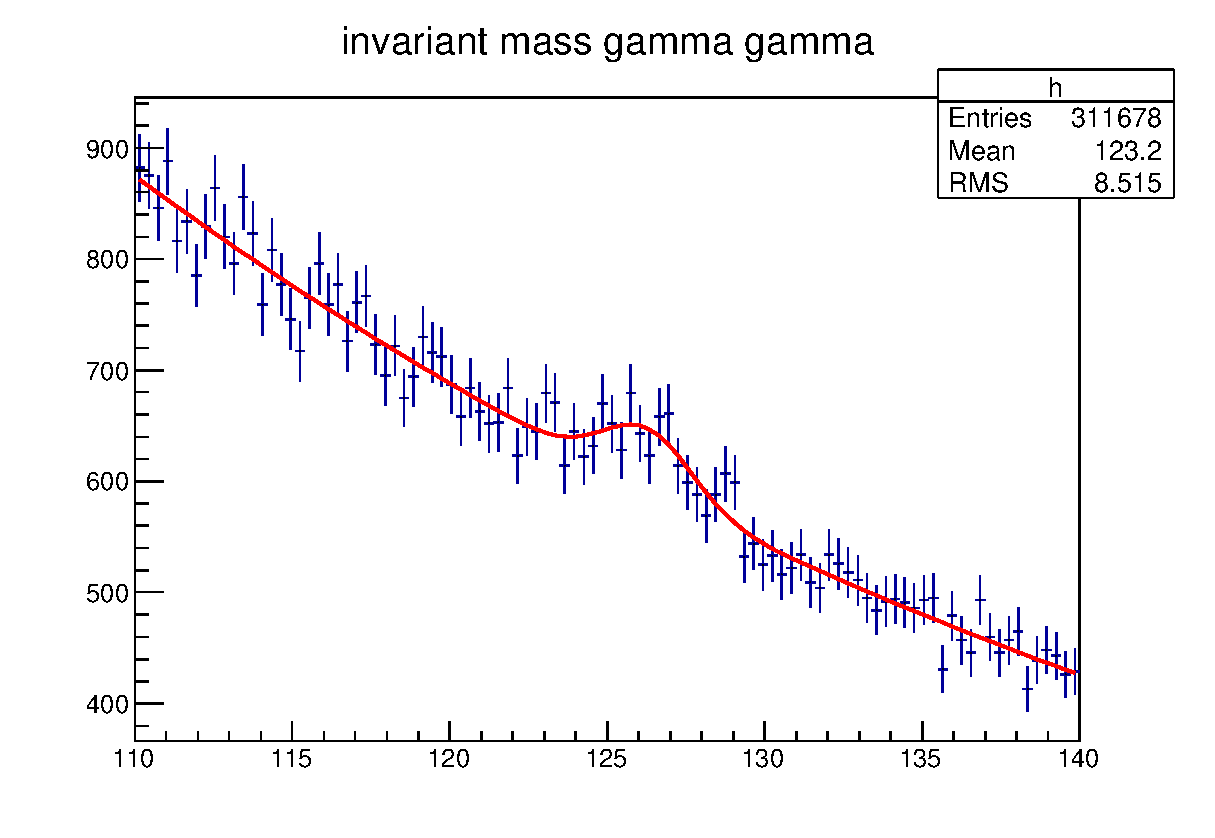
\includegraphics{../graphes/mgg_30GeV}
%\end{figure}
%
%On peut en déduire les paramètres physiquement intéressants suivants :
%
%\begin{tabular}{|l|c|r|} 
%   \hline
%   Paramètre & Valeur & Erreur \\
%    \hline
%   $E_0$ & 126,3 GeV & 0,3 GeV\\
%  \hline
%   $\sigma$ & 2,0 GeV & 0,9 GeV \\
%  \hline
%\end{tabular}
%
%La valeur $E_0$ doit correspondre à la masse du Higgs. On remarque qu'elle en est en effet bien proche (126 au lieu de 125 GeV). La valeur $\sigma$ doit correspondre à la largeur du signal, dont la valeur théorique attendue n'est pas nulle.
%
%On calcule de plus $\chi^2 = $ 68,8 pour un nombre de degrés de liberté égal à 99, ce qui correspond à une p-value de 99,0 \% (2,5$\sigma$?)
%$\Delta \chi^2 = \chi^2_{\textrm{background}} - \chi^2{\textrm{signal+background} \simeq 120-70 \simeq 50$ soit une significance à $\sqrt{\Delta \chi^2} \sigma = 7 \sigma$

Afin d'extraire le signal correspondant au Higgs, on se restreint à la plage où il est attendu (100 - 150 GeV). Le 'background' y suit une forme exponentielle. On en réalise alors un fit sur une zone ou le signal est considéré nul : ici on a choisi [100;120] $\cup$  [130;150]. On obtient une fonction de la forme $\textrm{background} = m_{\gamma\gamma} \mapsto \exp(\xi + \epsilon m_{\gamma\gamma})$.

Puis, sur la plage complète ([100, 150]), on réalise un fit des données à partir d'une fonction de la forme signal+background : $m_{\gamma\gamma} \mapsto  A \exp\left(-(m_{\gamma\gamma}-m_H)^2/2\sigma^2\right) + \exp(\xi + \epsilon m_{\gamma\gamma})$

On obtient la figure suivante :

\begin{figure}[H]
\centering
  \caption{Distribution $m_{\gamma \gamma}$ et fit background+signal. ($\sqrt{s} =$ 8 TeV,  $\int L dt$ = 20,3 fb$^{-1}$) }
 \resizebox{.9\linewidth}{!}{\begin{tikzpicture}
\pgfdeclareplotmark{cross} {
\pgfpathmoveto{\pgfpoint{-0.3\pgfplotmarksize}{\pgfplotmarksize}}
\pgfpathlineto{\pgfpoint{+0.3\pgfplotmarksize}{\pgfplotmarksize}}
\pgfpathlineto{\pgfpoint{+0.3\pgfplotmarksize}{0.3\pgfplotmarksize}}
\pgfpathlineto{\pgfpoint{+1\pgfplotmarksize}{0.3\pgfplotmarksize}}
\pgfpathlineto{\pgfpoint{+1\pgfplotmarksize}{-0.3\pgfplotmarksize}}
\pgfpathlineto{\pgfpoint{+0.3\pgfplotmarksize}{-0.3\pgfplotmarksize}}
\pgfpathlineto{\pgfpoint{+0.3\pgfplotmarksize}{-1.\pgfplotmarksize}}
\pgfpathlineto{\pgfpoint{-0.3\pgfplotmarksize}{-1.\pgfplotmarksize}}
\pgfpathlineto{\pgfpoint{-0.3\pgfplotmarksize}{-0.3\pgfplotmarksize}}
\pgfpathlineto{\pgfpoint{-1.\pgfplotmarksize}{-0.3\pgfplotmarksize}}
\pgfpathlineto{\pgfpoint{-1.\pgfplotmarksize}{0.3\pgfplotmarksize}}
\pgfpathlineto{\pgfpoint{-0.3\pgfplotmarksize}{0.3\pgfplotmarksize}}
\pgfpathclose
\pgfusepathqstroke
}
\pgfdeclareplotmark{cross*} {
\pgfpathmoveto{\pgfpoint{-0.3\pgfplotmarksize}{\pgfplotmarksize}}
\pgfpathlineto{\pgfpoint{+0.3\pgfplotmarksize}{\pgfplotmarksize}}
\pgfpathlineto{\pgfpoint{+0.3\pgfplotmarksize}{0.3\pgfplotmarksize}}
\pgfpathlineto{\pgfpoint{+1\pgfplotmarksize}{0.3\pgfplotmarksize}}
\pgfpathlineto{\pgfpoint{+1\pgfplotmarksize}{-0.3\pgfplotmarksize}}
\pgfpathlineto{\pgfpoint{+0.3\pgfplotmarksize}{-0.3\pgfplotmarksize}}
\pgfpathlineto{\pgfpoint{+0.3\pgfplotmarksize}{-1.\pgfplotmarksize}}
\pgfpathlineto{\pgfpoint{-0.3\pgfplotmarksize}{-1.\pgfplotmarksize}}
\pgfpathlineto{\pgfpoint{-0.3\pgfplotmarksize}{-0.3\pgfplotmarksize}}
\pgfpathlineto{\pgfpoint{-1.\pgfplotmarksize}{-0.3\pgfplotmarksize}}
\pgfpathlineto{\pgfpoint{-1.\pgfplotmarksize}{0.3\pgfplotmarksize}}
\pgfpathlineto{\pgfpoint{-0.3\pgfplotmarksize}{0.3\pgfplotmarksize}}
\pgfpathclose
\pgfusepathqfillstroke
}
\pgfdeclareplotmark{newstar} {
\pgfpathmoveto{\pgfqpoint{0pt}{\pgfplotmarksize}}
\pgfpathlineto{\pgfqpointpolar{44}{0.5\pgfplotmarksize}}
\pgfpathlineto{\pgfqpointpolar{18}{\pgfplotmarksize}}
\pgfpathlineto{\pgfqpointpolar{-20}{0.5\pgfplotmarksize}}
\pgfpathlineto{\pgfqpointpolar{-54}{\pgfplotmarksize}}
\pgfpathlineto{\pgfqpointpolar{-90}{0.5\pgfplotmarksize}}
\pgfpathlineto{\pgfqpointpolar{234}{\pgfplotmarksize}}
\pgfpathlineto{\pgfqpointpolar{198}{0.5\pgfplotmarksize}}
\pgfpathlineto{\pgfqpointpolar{162}{\pgfplotmarksize}}
\pgfpathlineto{\pgfqpointpolar{134}{0.5\pgfplotmarksize}}
\pgfpathclose
\pgfusepathqstroke
}
\pgfdeclareplotmark{newstar*} {
\pgfpathmoveto{\pgfqpoint{0pt}{\pgfplotmarksize}}
\pgfpathlineto{\pgfqpointpolar{44}{0.5\pgfplotmarksize}}
\pgfpathlineto{\pgfqpointpolar{18}{\pgfplotmarksize}}
\pgfpathlineto{\pgfqpointpolar{-20}{0.5\pgfplotmarksize}}
\pgfpathlineto{\pgfqpointpolar{-54}{\pgfplotmarksize}}
\pgfpathlineto{\pgfqpointpolar{-90}{0.5\pgfplotmarksize}}
\pgfpathlineto{\pgfqpointpolar{234}{\pgfplotmarksize}}
\pgfpathlineto{\pgfqpointpolar{198}{0.5\pgfplotmarksize}}
\pgfpathlineto{\pgfqpointpolar{162}{\pgfplotmarksize}}
\pgfpathlineto{\pgfqpointpolar{134}{0.5\pgfplotmarksize}}
\pgfpathclose
\pgfusepathqfillstroke
}
\definecolor{c}{rgb}{1,1,1};
\draw [color=c, fill=c] (0,0) rectangle (20,13.6207);
\draw [color=c, fill=c] (2,1.36207) rectangle (18,12.2586);
\definecolor{c}{rgb}{0,0,0};
\draw [c,line width=0.9] (2,1.36207) -- (2,12.2586) -- (18,12.2586) -- (18,1.36207) -- (2,1.36207);
\definecolor{c}{rgb}{1,1,1};
\draw [color=c, fill=c] (2,1.36207) rectangle (18,12.2586);
\definecolor{c}{rgb}{0,0,0};
\draw [c,line width=0.9] (2,1.36207) -- (2,12.2586) -- (18,12.2586) -- (18,1.36207) -- (2,1.36207);
\definecolor{c}{rgb}{0,0,0.6};
\draw [c,line width=0.9] (2.08,10.3742) -- (2.08,10.6675);
\draw [c,line width=0.9] (2.08,10.6675) -- (2.08,10.9608);
\draw [c,line width=0.9] (2,10.6675) -- (2.08,10.6675);
\draw [c,line width=0.9] (2.08,10.6675) -- (2.16,10.6675);
\definecolor{c}{rgb}{0,0,0};
\foreach \P in {(2.08,10.6675)}{\draw[mark options={color=c,fill=c},mark size=2.402402pt,mark=*,mark size=1pt] plot coordinates {\P};}
\definecolor{c}{rgb}{0,0,0.6};
\draw [c,line width=0.9] (2.24,11.1352) -- (2.24,11.4375);
\draw [c,line width=0.9] (2.24,11.4375) -- (2.24,11.7397);
\draw [c,line width=0.9] (2.16,11.4375) -- (2.24,11.4375);
\draw [c,line width=0.9] (2.24,11.4375) -- (2.32,11.4375);
\definecolor{c}{rgb}{0,0,0};
\foreach \P in {(2.24,11.4375)}{\draw[mark options={color=c,fill=c},mark size=2.402402pt,mark=*,mark size=1pt] plot coordinates {\P};}
\definecolor{c}{rgb}{0,0,0.6};
\draw [c,line width=0.9] (2.4,9.90813) -- (2.4,10.1958);
\draw [c,line width=0.9] (2.4,10.1958) -- (2.4,10.4835);
\draw [c,line width=0.9] (2.32,10.1958) -- (2.4,10.1958);
\draw [c,line width=0.9] (2.4,10.1958) -- (2.48,10.1958);
\definecolor{c}{rgb}{0,0,0};
\foreach \P in {(2.4,10.1958)}{\draw[mark options={color=c,fill=c},mark size=2.402402pt,mark=*,mark size=1pt] plot coordinates {\P};}
\definecolor{c}{rgb}{0,0,0.6};
\draw [c,line width=0.9] (2.56,10.1137) -- (2.56,10.4039);
\draw [c,line width=0.9] (2.56,10.4039) -- (2.56,10.6941);
\draw [c,line width=0.9] (2.48,10.4039) -- (2.56,10.4039);
\draw [c,line width=0.9] (2.56,10.4039) -- (2.64,10.4039);
\definecolor{c}{rgb}{0,0,0};
\foreach \P in {(2.56,10.4039)}{\draw[mark options={color=c,fill=c},mark size=2.402402pt,mark=*,mark size=1pt] plot coordinates {\P};}
\definecolor{c}{rgb}{0,0,0.6};
\draw [c,line width=0.9] (2.72,10.3536) -- (2.72,10.6467);
\draw [c,line width=0.9] (2.72,10.6467) -- (2.72,10.9398);
\draw [c,line width=0.9] (2.64,10.6467) -- (2.72,10.6467);
\draw [c,line width=0.9] (2.72,10.6467) -- (2.8,10.6467);
\definecolor{c}{rgb}{0,0,0};
\foreach \P in {(2.72,10.6467)}{\draw[mark options={color=c,fill=c},mark size=2.402402pt,mark=*,mark size=1pt] plot coordinates {\P};}
\definecolor{c}{rgb}{0,0,0.6};
\draw [c,line width=0.9] (2.88,10.0041) -- (2.88,10.2929);
\draw [c,line width=0.9] (2.88,10.2929) -- (2.88,10.5818);
\draw [c,line width=0.9] (2.8,10.2929) -- (2.88,10.2929);
\draw [c,line width=0.9] (2.88,10.2929) -- (2.96,10.2929);
\definecolor{c}{rgb}{0,0,0};
\foreach \P in {(2.88,10.2929)}{\draw[mark options={color=c,fill=c},mark size=2.402402pt,mark=*,mark size=1pt] plot coordinates {\P};}
\definecolor{c}{rgb}{0,0,0.6};
\draw [c,line width=0.9] (3.04,9.53811) -- (3.04,9.82124);
\draw [c,line width=0.9] (3.04,9.82124) -- (3.04,10.1044);
\draw [c,line width=0.9] (2.96,9.82124) -- (3.04,9.82124);
\draw [c,line width=0.9] (3.04,9.82124) -- (3.12,9.82124);
\definecolor{c}{rgb}{0,0,0};
\foreach \P in {(3.04,9.82124)}{\draw[mark options={color=c,fill=c},mark size=2.402402pt,mark=*,mark size=1pt] plot coordinates {\P};}
\definecolor{c}{rgb}{0,0,0.6};
\draw [c,line width=0.9] (3.2,9.5107) -- (3.2,9.79349);
\draw [c,line width=0.9] (3.2,9.79349) -- (3.2,10.0763);
\draw [c,line width=0.9] (3.12,9.79349) -- (3.2,9.79349);
\draw [c,line width=0.9] (3.2,9.79349) -- (3.28,9.79349);
\definecolor{c}{rgb}{0,0,0};
\foreach \P in {(3.2,9.79349)}{\draw[mark options={color=c,fill=c},mark size=2.402402pt,mark=*,mark size=1pt] plot coordinates {\P};}
\definecolor{c}{rgb}{0,0,0.6};
\draw [c,line width=0.9] (3.36,9.54496) -- (3.36,9.82817);
\draw [c,line width=0.9] (3.36,9.82817) -- (3.36,10.1114);
\draw [c,line width=0.9] (3.28,9.82817) -- (3.36,9.82817);
\draw [c,line width=0.9] (3.36,9.82817) -- (3.44,9.82817);
\definecolor{c}{rgb}{0,0,0};
\foreach \P in {(3.36,9.82817)}{\draw[mark options={color=c,fill=c},mark size=2.402402pt,mark=*,mark size=1pt] plot coordinates {\P};}
\definecolor{c}{rgb}{0,0,0.6};
\draw [c,line width=0.9] (3.52,9.97666) -- (3.52,10.2652);
\draw [c,line width=0.9] (3.52,10.2652) -- (3.52,10.5537);
\draw [c,line width=0.9] (3.44,10.2652) -- (3.52,10.2652);
\draw [c,line width=0.9] (3.52,10.2652) -- (3.6,10.2652);
\definecolor{c}{rgb}{0,0,0};
\foreach \P in {(3.52,10.2652)}{\draw[mark options={color=c,fill=c},mark size=2.402402pt,mark=*,mark size=1pt] plot coordinates {\P};}
\definecolor{c}{rgb}{0,0,0.6};
\draw [c,line width=0.9] (3.68,9.44219) -- (3.68,9.72412);
\draw [c,line width=0.9] (3.68,9.72412) -- (3.68,10.0061);
\draw [c,line width=0.9] (3.6,9.72412) -- (3.68,9.72412);
\draw [c,line width=0.9] (3.68,9.72412) -- (3.76,9.72412);
\definecolor{c}{rgb}{0,0,0};
\foreach \P in {(3.68,9.72412)}{\draw[mark options={color=c,fill=c},mark size=2.402402pt,mark=*,mark size=1pt] plot coordinates {\P};}
\definecolor{c}{rgb}{0,0,0.6};
\draw [c,line width=0.9] (3.84,9.33257) -- (3.84,9.61314);
\draw [c,line width=0.9] (3.84,9.61314) -- (3.84,9.89371);
\draw [c,line width=0.9] (3.76,9.61314) -- (3.84,9.61314);
\draw [c,line width=0.9] (3.84,9.61314) -- (3.92,9.61314);
\definecolor{c}{rgb}{0,0,0};
\foreach \P in {(3.84,9.61314)}{\draw[mark options={color=c,fill=c},mark size=2.402402pt,mark=*,mark size=1pt] plot coordinates {\P};}
\definecolor{c}{rgb}{0,0,0.6};
\draw [c,line width=0.9] (4,9.18186) -- (4,9.46053);
\draw [c,line width=0.9] (4,9.46053) -- (4,9.73921);
\draw [c,line width=0.9] (3.92,9.46053) -- (4,9.46053);
\draw [c,line width=0.9] (4,9.46053) -- (4.08,9.46053);
\definecolor{c}{rgb}{0,0,0};
\foreach \P in {(4,9.46053)}{\draw[mark options={color=c,fill=c},mark size=2.402402pt,mark=*,mark size=1pt] plot coordinates {\P};}
\definecolor{c}{rgb}{0,0,0.6};
\draw [c,line width=0.9] (4.16,8.4285) -- (4.16,8.69751);
\draw [c,line width=0.9] (4.16,8.69751) -- (4.16,8.96652);
\draw [c,line width=0.9] (4.08,8.69751) -- (4.16,8.69751);
\draw [c,line width=0.9] (4.16,8.69751) -- (4.24,8.69751);
\definecolor{c}{rgb}{0,0,0};
\foreach \P in {(4.16,8.69751)}{\draw[mark options={color=c,fill=c},mark size=2.402402pt,mark=*,mark size=1pt] plot coordinates {\P};}
\definecolor{c}{rgb}{0,0,0.6};
\draw [c,line width=0.9] (4.32,8.61338) -- (4.32,8.8848);
\draw [c,line width=0.9] (4.32,8.8848) -- (4.32,9.15621);
\draw [c,line width=0.9] (4.24,8.8848) -- (4.32,8.8848);
\draw [c,line width=0.9] (4.32,8.8848) -- (4.4,8.8848);
\definecolor{c}{rgb}{0,0,0};
\foreach \P in {(4.32,8.8848)}{\draw[mark options={color=c,fill=c},mark size=2.402402pt,mark=*,mark size=1pt] plot coordinates {\P};}
\definecolor{c}{rgb}{0,0,0.6};
\draw [c,line width=0.9] (4.48,8.5449) -- (4.48,8.81543);
\draw [c,line width=0.9] (4.48,8.81543) -- (4.48,9.08596);
\draw [c,line width=0.9] (4.4,8.81543) -- (4.48,8.81543);
\draw [c,line width=0.9] (4.48,8.81543) -- (4.56,8.81543);
\definecolor{c}{rgb}{0,0,0};
\foreach \P in {(4.48,8.81543)}{\draw[mark options={color=c,fill=c},mark size=2.402402pt,mark=*,mark size=1pt] plot coordinates {\P};}
\definecolor{c}{rgb}{0,0,0.6};
\draw [c,line width=0.9] (4.64,8.68871) -- (4.64,8.9611);
\draw [c,line width=0.9] (4.64,8.9611) -- (4.64,9.23349);
\draw [c,line width=0.9] (4.56,8.9611) -- (4.64,8.9611);
\draw [c,line width=0.9] (4.64,8.9611) -- (4.72,8.9611);
\definecolor{c}{rgb}{0,0,0};
\foreach \P in {(4.64,8.9611)}{\draw[mark options={color=c,fill=c},mark size=2.402402pt,mark=*,mark size=1pt] plot coordinates {\P};}
\definecolor{c}{rgb}{0,0,0.6};
\draw [c,line width=0.9] (4.8,8.33949) -- (4.8,8.60733);
\draw [c,line width=0.9] (4.8,8.60733) -- (4.8,8.87518);
\draw [c,line width=0.9] (4.72,8.60733) -- (4.8,8.60733);
\draw [c,line width=0.9] (4.8,8.60733) -- (4.88,8.60733);
\definecolor{c}{rgb}{0,0,0};
\foreach \P in {(4.8,8.60733)}{\draw[mark options={color=c,fill=c},mark size=2.402402pt,mark=*,mark size=1pt] plot coordinates {\P};}
\definecolor{c}{rgb}{0,0,0.6};
\draw [c,line width=0.9] (4.96,8.09303) -- (4.96,8.35762);
\draw [c,line width=0.9] (4.96,8.35762) -- (4.96,8.62221);
\draw [c,line width=0.9] (4.88,8.35762) -- (4.96,8.35762);
\draw [c,line width=0.9] (4.96,8.35762) -- (5.04,8.35762);
\definecolor{c}{rgb}{0,0,0};
\foreach \P in {(4.96,8.35762)}{\draw[mark options={color=c,fill=c},mark size=2.402402pt,mark=*,mark size=1pt] plot coordinates {\P};}
\definecolor{c}{rgb}{0,0,0.6};
\draw [c,line width=0.9] (5.12,8.63393) -- (5.12,8.90561);
\draw [c,line width=0.9] (5.12,8.90561) -- (5.12,9.17729);
\draw [c,line width=0.9] (5.04,8.90561) -- (5.12,8.90561);
\draw [c,line width=0.9] (5.12,8.90561) -- (5.2,8.90561);
\definecolor{c}{rgb}{0,0,0};
\foreach \P in {(5.12,8.90561)}{\draw[mark options={color=c,fill=c},mark size=2.402402pt,mark=*,mark size=1pt] plot coordinates {\P};}
\definecolor{c}{rgb}{0,0,0.6};
\draw [c,line width=0.9] (5.28,8.09987) -- (5.28,8.36455);
\draw [c,line width=0.9] (5.28,8.36455) -- (5.28,8.62924);
\draw [c,line width=0.9] (5.2,8.36455) -- (5.28,8.36455);
\draw [c,line width=0.9] (5.28,8.36455) -- (5.36,8.36455);
\definecolor{c}{rgb}{0,0,0};
\foreach \P in {(5.28,8.36455)}{\draw[mark options={color=c,fill=c},mark size=2.402402pt,mark=*,mark size=1pt] plot coordinates {\P};}
\definecolor{c}{rgb}{0,0,0.6};
\draw [c,line width=0.9] (5.44,8.20256) -- (5.44,8.4686);
\draw [c,line width=0.9] (5.44,8.4686) -- (5.44,8.73464);
\draw [c,line width=0.9] (5.36,8.4686) -- (5.44,8.4686);
\draw [c,line width=0.9] (5.44,8.4686) -- (5.52,8.4686);
\definecolor{c}{rgb}{0,0,0};
\foreach \P in {(5.44,8.4686)}{\draw[mark options={color=c,fill=c},mark size=2.402402pt,mark=*,mark size=1pt] plot coordinates {\P};}
\definecolor{c}{rgb}{0,0,0.6};
\draw [c,line width=0.9] (5.6,7.57969) -- (5.6,7.83737);
\draw [c,line width=0.9] (5.6,7.83737) -- (5.6,8.09506);
\draw [c,line width=0.9] (5.52,7.83737) -- (5.6,7.83737);
\draw [c,line width=0.9] (5.6,7.83737) -- (5.68,7.83737);
\definecolor{c}{rgb}{0,0,0};
\foreach \P in {(5.6,7.83737)}{\draw[mark options={color=c,fill=c},mark size=2.402402pt,mark=*,mark size=1pt] plot coordinates {\P};}
\definecolor{c}{rgb}{0,0,0.6};
\draw [c,line width=0.9] (5.76,7.49758) -- (5.76,7.75413);
\draw [c,line width=0.9] (5.76,7.75413) -- (5.76,8.01069);
\draw [c,line width=0.9] (5.68,7.75413) -- (5.76,7.75413);
\draw [c,line width=0.9] (5.76,7.75413) -- (5.84,7.75413);
\definecolor{c}{rgb}{0,0,0};
\foreach \P in {(5.76,7.75413)}{\draw[mark options={color=c,fill=c},mark size=2.402402pt,mark=*,mark size=1pt] plot coordinates {\P};}
\definecolor{c}{rgb}{0,0,0.6};
\draw [c,line width=0.9] (5.92,7.4702) -- (5.92,7.72639);
\draw [c,line width=0.9] (5.92,7.72639) -- (5.92,7.98257);
\draw [c,line width=0.9] (5.84,7.72639) -- (5.92,7.72639);
\draw [c,line width=0.9] (5.92,7.72639) -- (6,7.72639);
\definecolor{c}{rgb}{0,0,0};
\foreach \P in {(5.92,7.72639)}{\draw[mark options={color=c,fill=c},mark size=2.402402pt,mark=*,mark size=1pt] plot coordinates {\P};}
\definecolor{c}{rgb}{0,0,0.6};
\draw [c,line width=0.9] (6.08,7.71656) -- (6.08,7.97611);
\draw [c,line width=0.9] (6.08,7.97611) -- (6.08,8.23565);
\draw [c,line width=0.9] (6,7.97611) -- (6.08,7.97611);
\draw [c,line width=0.9] (6.08,7.97611) -- (6.16,7.97611);
\definecolor{c}{rgb}{0,0,0};
\foreach \P in {(6.08,7.97611)}{\draw[mark options={color=c,fill=c},mark size=2.402402pt,mark=*,mark size=1pt] plot coordinates {\P};}
\definecolor{c}{rgb}{0,0,0.6};
\draw [c,line width=0.9] (6.24,7.57969) -- (6.24,7.83737);
\draw [c,line width=0.9] (6.24,7.83737) -- (6.24,8.09506);
\draw [c,line width=0.9] (6.16,7.83737) -- (6.24,7.83737);
\draw [c,line width=0.9] (6.24,7.83737) -- (6.32,7.83737);
\definecolor{c}{rgb}{0,0,0};
\foreach \P in {(6.24,7.83737)}{\draw[mark options={color=c,fill=c},mark size=2.402402pt,mark=*,mark size=1pt] plot coordinates {\P};}
\definecolor{c}{rgb}{0,0,0.6};
\draw [c,line width=0.9] (6.4,7.53179) -- (6.4,7.78882);
\draw [c,line width=0.9] (6.4,7.78882) -- (6.4,8.04585);
\draw [c,line width=0.9] (6.32,7.78882) -- (6.4,7.78882);
\draw [c,line width=0.9] (6.4,7.78882) -- (6.48,7.78882);
\definecolor{c}{rgb}{0,0,0};
\foreach \P in {(6.4,7.78882)}{\draw[mark options={color=c,fill=c},mark size=2.402402pt,mark=*,mark size=1pt] plot coordinates {\P};}
\definecolor{c}{rgb}{0,0,0.6};
\draw [c,line width=0.9] (6.56,6.9571) -- (6.56,7.20615);
\draw [c,line width=0.9] (6.56,7.20615) -- (6.56,7.45519);
\draw [c,line width=0.9] (6.48,7.20615) -- (6.56,7.20615);
\draw [c,line width=0.9] (6.56,7.20615) -- (6.64,7.20615);
\definecolor{c}{rgb}{0,0,0};
\foreach \P in {(6.56,7.20615)}{\draw[mark options={color=c,fill=c},mark size=2.402402pt,mark=*,mark size=1pt] plot coordinates {\P};}
\definecolor{c}{rgb}{0,0,0.6};
\draw [c,line width=0.9] (6.72,6.7656) -- (6.72,7.01192);
\draw [c,line width=0.9] (6.72,7.01192) -- (6.72,7.25824);
\draw [c,line width=0.9] (6.64,7.01192) -- (6.72,7.01192);
\draw [c,line width=0.9] (6.72,7.01192) -- (6.8,7.01192);
\definecolor{c}{rgb}{0,0,0};
\foreach \P in {(6.72,7.01192)}{\draw[mark options={color=c,fill=c},mark size=2.402402pt,mark=*,mark size=1pt] plot coordinates {\P};}
\definecolor{c}{rgb}{0,0,0.6};
\draw [c,line width=0.9] (6.88,6.44421) -- (6.88,6.6859);
\draw [c,line width=0.9] (6.88,6.6859) -- (6.88,6.92759);
\draw [c,line width=0.9] (6.8,6.6859) -- (6.88,6.6859);
\draw [c,line width=0.9] (6.88,6.6859) -- (6.96,6.6859);
\definecolor{c}{rgb}{0,0,0};
\foreach \P in {(6.88,6.6859)}{\draw[mark options={color=c,fill=c},mark size=2.402402pt,mark=*,mark size=1pt] plot coordinates {\P};}
\definecolor{c}{rgb}{0,0,0.6};
\draw [c,line width=0.9] (7.04,7.21021) -- (7.04,7.4628);
\draw [c,line width=0.9] (7.04,7.4628) -- (7.04,7.71539);
\draw [c,line width=0.9] (6.96,7.4628) -- (7.04,7.4628);
\draw [c,line width=0.9] (7.04,7.4628) -- (7.12,7.4628);
\definecolor{c}{rgb}{0,0,0};
\foreach \P in {(7.04,7.4628)}{\draw[mark options={color=c,fill=c},mark size=2.402402pt,mark=*,mark size=1pt] plot coordinates {\P};}
\definecolor{c}{rgb}{0,0,0.6};
\draw [c,line width=0.9] (7.2,6.92974) -- (7.2,7.1784);
\draw [c,line width=0.9] (7.2,7.1784) -- (7.2,7.42705);
\draw [c,line width=0.9] (7.12,7.1784) -- (7.2,7.1784);
\draw [c,line width=0.9] (7.2,7.1784) -- (7.28,7.1784);
\definecolor{c}{rgb}{0,0,0};
\foreach \P in {(7.2,7.1784)}{\draw[mark options={color=c,fill=c},mark size=2.402402pt,mark=*,mark size=1pt] plot coordinates {\P};}
\definecolor{c}{rgb}{0,0,0.6};
\draw [c,line width=0.9] (7.36,6.60148) -- (7.36,6.84544);
\draw [c,line width=0.9] (7.36,6.84544) -- (7.36,7.08941);
\draw [c,line width=0.9] (7.28,6.84544) -- (7.36,6.84544);
\draw [c,line width=0.9] (7.36,6.84544) -- (7.44,6.84544);
\definecolor{c}{rgb}{0,0,0};
\foreach \P in {(7.36,6.84544)}{\draw[mark options={color=c,fill=c},mark size=2.402402pt,mark=*,mark size=1pt] plot coordinates {\P};}
\definecolor{c}{rgb}{0,0,0.6};
\draw [c,line width=0.9] (7.52,6.81347) -- (7.52,7.06048);
\draw [c,line width=0.9] (7.52,7.06048) -- (7.52,7.30748);
\draw [c,line width=0.9] (7.44,7.06048) -- (7.52,7.06048);
\draw [c,line width=0.9] (7.52,7.06048) -- (7.6,7.06048);
\definecolor{c}{rgb}{0,0,0};
\foreach \P in {(7.52,7.06048)}{\draw[mark options={color=c,fill=c},mark size=2.402402pt,mark=*,mark size=1pt] plot coordinates {\P};}
\definecolor{c}{rgb}{0,0,0.6};
\draw [c,line width=0.9] (7.68,6.21178) -- (7.68,6.45006);
\draw [c,line width=0.9] (7.68,6.45006) -- (7.68,6.68834);
\draw [c,line width=0.9] (7.6,6.45006) -- (7.68,6.45006);
\draw [c,line width=0.9] (7.68,6.45006) -- (7.76,6.45006);
\definecolor{c}{rgb}{0,0,0};
\foreach \P in {(7.68,6.45006)}{\draw[mark options={color=c,fill=c},mark size=2.402402pt,mark=*,mark size=1pt] plot coordinates {\P};}
\definecolor{c}{rgb}{0,0,0.6};
\draw [c,line width=0.9] (7.84,6.25279) -- (7.84,6.49168);
\draw [c,line width=0.9] (7.84,6.49168) -- (7.84,6.73056);
\draw [c,line width=0.9] (7.76,6.49168) -- (7.84,6.49168);
\draw [c,line width=0.9] (7.84,6.49168) -- (7.92,6.49168);
\definecolor{c}{rgb}{0,0,0};
\foreach \P in {(7.84,6.49168)}{\draw[mark options={color=c,fill=c},mark size=2.402402pt,mark=*,mark size=1pt] plot coordinates {\P};}
\definecolor{c}{rgb}{0,0,0.6};
\draw [c,line width=0.9] (8,5.95889) -- (8,6.1934);
\draw [c,line width=0.9] (8,6.1934) -- (8,6.42792);
\draw [c,line width=0.9] (7.92,6.1934) -- (8,6.1934);
\draw [c,line width=0.9] (8,6.1934) -- (8.08,6.1934);
\definecolor{c}{rgb}{0,0,0};
\foreach \P in {(8,6.1934)}{\draw[mark options={color=c,fill=c},mark size=2.402402pt,mark=*,mark size=1pt] plot coordinates {\P};}
\definecolor{c}{rgb}{0,0,0.6};
\draw [c,line width=0.9] (8.16,6.5878) -- (8.16,6.83157);
\draw [c,line width=0.9] (8.16,6.83157) -- (8.16,7.07534);
\draw [c,line width=0.9] (8.08,6.83157) -- (8.16,6.83157);
\draw [c,line width=0.9] (8.16,6.83157) -- (8.24,6.83157);
\definecolor{c}{rgb}{0,0,0};
\foreach \P in {(8.16,6.83157)}{\draw[mark options={color=c,fill=c},mark size=2.402402pt,mark=*,mark size=1pt] plot coordinates {\P};}
\definecolor{c}{rgb}{0,0,0.6};
\draw [c,line width=0.9] (8.32,6.10241) -- (8.32,6.33907);
\draw [c,line width=0.9] (8.32,6.33907) -- (8.32,6.57573);
\draw [c,line width=0.9] (8.24,6.33907) -- (8.32,6.33907);
\draw [c,line width=0.9] (8.32,6.33907) -- (8.4,6.33907);
\definecolor{c}{rgb}{0,0,0};
\foreach \P in {(8.32,6.33907)}{\draw[mark options={color=c,fill=c},mark size=2.402402pt,mark=*,mark size=1pt] plot coordinates {\P};}
\definecolor{c}{rgb}{0,0,0.6};
\draw [c,line width=0.9] (8.48,5.6924) -- (8.48,5.92288);
\draw [c,line width=0.9] (8.48,5.92288) -- (8.48,6.15336);
\draw [c,line width=0.9] (8.4,5.92288) -- (8.48,5.92288);
\draw [c,line width=0.9] (8.48,5.92288) -- (8.56,5.92288);
\definecolor{c}{rgb}{0,0,0};
\foreach \P in {(8.48,5.92288)}{\draw[mark options={color=c,fill=c},mark size=2.402402pt,mark=*,mark size=1pt] plot coordinates {\P};}
\definecolor{c}{rgb}{0,0,0.6};
\draw [c,line width=0.9] (8.64,5.80172) -- (8.64,6.03386);
\draw [c,line width=0.9] (8.64,6.03386) -- (8.64,6.26601);
\draw [c,line width=0.9] (8.56,6.03386) -- (8.64,6.03386);
\draw [c,line width=0.9] (8.64,6.03386) -- (8.72,6.03386);
\definecolor{c}{rgb}{0,0,0};
\foreach \P in {(8.64,6.03386)}{\draw[mark options={color=c,fill=c},mark size=2.402402pt,mark=*,mark size=1pt] plot coordinates {\P};}
\definecolor{c}{rgb}{0,0,0.6};
\draw [c,line width=0.9] (8.8,5.55577) -- (8.8,5.78415);
\draw [c,line width=0.9] (8.8,5.78415) -- (8.8,6.01253);
\draw [c,line width=0.9] (8.72,5.78415) -- (8.8,5.78415);
\draw [c,line width=0.9] (8.8,5.78415) -- (8.88,5.78415);
\definecolor{c}{rgb}{0,0,0};
\foreach \P in {(8.8,5.78415)}{\draw[mark options={color=c,fill=c},mark size=2.402402pt,mark=*,mark size=1pt] plot coordinates {\P};}
\definecolor{c}{rgb}{0,0,0.6};
\draw [c,line width=0.9] (8.96,5.88372) -- (8.96,6.1171);
\draw [c,line width=0.9] (8.96,6.1171) -- (8.96,6.35048);
\draw [c,line width=0.9] (8.88,6.1171) -- (8.96,6.1171);
\draw [c,line width=0.9] (8.96,6.1171) -- (9.04,6.1171);
\definecolor{c}{rgb}{0,0,0};
\foreach \P in {(8.96,6.1171)}{\draw[mark options={color=c,fill=c},mark size=2.402402pt,mark=*,mark size=1pt] plot coordinates {\P};}
\definecolor{c}{rgb}{0,0,0.6};
\draw [c,line width=0.9] (9.12,5.385) -- (9.12,5.61073);
\draw [c,line width=0.9] (9.12,5.61073) -- (9.12,5.83646);
\draw [c,line width=0.9] (9.04,5.61073) -- (9.12,5.61073);
\draw [c,line width=0.9] (9.12,5.61073) -- (9.2,5.61073);
\definecolor{c}{rgb}{0,0,0};
\foreach \P in {(9.12,5.61073)}{\draw[mark options={color=c,fill=c},mark size=2.402402pt,mark=*,mark size=1pt] plot coordinates {\P};}
\definecolor{c}{rgb}{0,0,0.6};
\draw [c,line width=0.9] (9.28,5.6719) -- (9.28,5.90207);
\draw [c,line width=0.9] (9.28,5.90207) -- (9.28,6.13223);
\draw [c,line width=0.9] (9.2,5.90207) -- (9.28,5.90207);
\draw [c,line width=0.9] (9.28,5.90207) -- (9.36,5.90207);
\definecolor{c}{rgb}{0,0,0};
\foreach \P in {(9.28,5.90207)}{\draw[mark options={color=c,fill=c},mark size=2.402402pt,mark=*,mark size=1pt] plot coordinates {\P};}
\definecolor{c}{rgb}{0,0,0.6};
\draw [c,line width=0.9] (9.44,5.7129) -- (9.44,5.94369);
\draw [c,line width=0.9] (9.44,5.94369) -- (9.44,6.17448);
\draw [c,line width=0.9] (9.36,5.94369) -- (9.44,5.94369);
\draw [c,line width=0.9] (9.44,5.94369) -- (9.52,5.94369);
\definecolor{c}{rgb}{0,0,0};
\foreach \P in {(9.44,5.94369)}{\draw[mark options={color=c,fill=c},mark size=2.402402pt,mark=*,mark size=1pt] plot coordinates {\P};}
\definecolor{c}{rgb}{0,0,0.6};
\draw [c,line width=0.9] (9.6,5.16647) -- (9.6,5.38876);
\draw [c,line width=0.9] (9.6,5.38876) -- (9.6,5.61106);
\draw [c,line width=0.9] (9.52,5.38876) -- (9.6,5.38876);
\draw [c,line width=0.9] (9.6,5.38876) -- (9.68,5.38876);
\definecolor{c}{rgb}{0,0,0};
\foreach \P in {(9.6,5.38876)}{\draw[mark options={color=c,fill=c},mark size=2.402402pt,mark=*,mark size=1pt] plot coordinates {\P};}
\definecolor{c}{rgb}{0,0,0.6};
\draw [c,line width=0.9] (9.76,5.46696) -- (9.76,5.69397);
\draw [c,line width=0.9] (9.76,5.69397) -- (9.76,5.92098);
\draw [c,line width=0.9] (9.68,5.69397) -- (9.76,5.69397);
\draw [c,line width=0.9] (9.76,5.69397) -- (9.84,5.69397);
\definecolor{c}{rgb}{0,0,0};
\foreach \P in {(9.76,5.69397)}{\draw[mark options={color=c,fill=c},mark size=2.402402pt,mark=*,mark size=1pt] plot coordinates {\P};}
\definecolor{c}{rgb}{0,0,0.6};
\draw [c,line width=0.9] (9.92,5.5626) -- (9.92,5.79108);
\draw [c,line width=0.9] (9.92,5.79108) -- (9.92,6.01957);
\draw [c,line width=0.9] (9.84,5.79108) -- (9.92,5.79108);
\draw [c,line width=0.9] (9.92,5.79108) -- (10,5.79108);
\definecolor{c}{rgb}{0,0,0};
\foreach \P in {(9.92,5.79108)}{\draw[mark options={color=c,fill=c},mark size=2.402402pt,mark=*,mark size=1pt] plot coordinates {\P};}
\definecolor{c}{rgb}{0,0,0.6};
\draw [c,line width=0.9] (10.08,5.48063) -- (10.08,5.70784);
\draw [c,line width=0.9] (10.08,5.70784) -- (10.08,5.93506);
\draw [c,line width=0.9] (10,5.70784) -- (10.08,5.70784);
\draw [c,line width=0.9] (10.08,5.70784) -- (10.16,5.70784);
\definecolor{c}{rgb}{0,0,0};
\foreach \P in {(10.08,5.70784)}{\draw[mark options={color=c,fill=c},mark size=2.402402pt,mark=*,mark size=1pt] plot coordinates {\P};}
\definecolor{c}{rgb}{0,0,0.6};
\draw [c,line width=0.9] (10.24,5.78806) -- (10.24,6.01999);
\draw [c,line width=0.9] (10.24,6.01999) -- (10.24,6.25192);
\draw [c,line width=0.9] (10.16,6.01999) -- (10.24,6.01999);
\draw [c,line width=0.9] (10.24,6.01999) -- (10.32,6.01999);
\definecolor{c}{rgb}{0,0,0};
\foreach \P in {(10.24,6.01999)}{\draw[mark options={color=c,fill=c},mark size=2.402402pt,mark=*,mark size=1pt] plot coordinates {\P};}
\definecolor{c}{rgb}{0,0,0.6};
\draw [c,line width=0.9] (10.4,5.21427) -- (10.4,5.43732);
\draw [c,line width=0.9] (10.4,5.43732) -- (10.4,5.66037);
\draw [c,line width=0.9] (10.32,5.43732) -- (10.4,5.43732);
\draw [c,line width=0.9] (10.4,5.43732) -- (10.48,5.43732);
\definecolor{c}{rgb}{0,0,0};
\foreach \P in {(10.4,5.43732)}{\draw[mark options={color=c,fill=c},mark size=2.402402pt,mark=*,mark size=1pt] plot coordinates {\P};}
\definecolor{c}{rgb}{0,0,0.6};
\draw [c,line width=0.9] (10.56,5.51478) -- (10.56,5.74253);
\draw [c,line width=0.9] (10.56,5.74253) -- (10.56,5.97027);
\draw [c,line width=0.9] (10.48,5.74253) -- (10.56,5.74253);
\draw [c,line width=0.9] (10.56,5.74253) -- (10.64,5.74253);
\definecolor{c}{rgb}{0,0,0};
\foreach \P in {(10.56,5.74253)}{\draw[mark options={color=c,fill=c},mark size=2.402402pt,mark=*,mark size=1pt] plot coordinates {\P};}
\definecolor{c}{rgb}{0,0,0.6};
\draw [c,line width=0.9] (10.72,5.36451) -- (10.72,5.58992);
\draw [c,line width=0.9] (10.72,5.58992) -- (10.72,5.81533);
\draw [c,line width=0.9] (10.64,5.58992) -- (10.72,5.58992);
\draw [c,line width=0.9] (10.72,5.58992) -- (10.8,5.58992);
\definecolor{c}{rgb}{0,0,0};
\foreach \P in {(10.72,5.58992)}{\draw[mark options={color=c,fill=c},mark size=2.402402pt,mark=*,mark size=1pt] plot coordinates {\P};}
\definecolor{c}{rgb}{0,0,0.6};
\draw [c,line width=0.9] (10.88,4.88655) -- (10.88,5.10436);
\draw [c,line width=0.9] (10.88,5.10436) -- (10.88,5.32218);
\draw [c,line width=0.9] (10.8,5.10436) -- (10.88,5.10436);
\draw [c,line width=0.9] (10.88,5.10436) -- (10.96,5.10436);
\definecolor{c}{rgb}{0,0,0};
\foreach \P in {(10.88,5.10436)}{\draw[mark options={color=c,fill=c},mark size=2.402402pt,mark=*,mark size=1pt] plot coordinates {\P};}
\definecolor{c}{rgb}{0,0,0.6};
\draw [c,line width=0.9] (11.04,4.75004) -- (11.04,4.96563);
\draw [c,line width=0.9] (11.04,4.96563) -- (11.04,5.18122);
\draw [c,line width=0.9] (10.96,4.96563) -- (11.04,4.96563);
\draw [c,line width=0.9] (11.04,4.96563) -- (11.12,4.96563);
\definecolor{c}{rgb}{0,0,0};
\foreach \P in {(11.04,4.96563)}{\draw[mark options={color=c,fill=c},mark size=2.402402pt,mark=*,mark size=1pt] plot coordinates {\P};}
\definecolor{c}{rgb}{0,0,0.6};
\draw [c,line width=0.9] (11.2,5.07087) -- (11.2,5.29165);
\draw [c,line width=0.9] (11.2,5.29165) -- (11.2,5.51242);
\draw [c,line width=0.9] (11.12,5.29165) -- (11.2,5.29165);
\draw [c,line width=0.9] (11.2,5.29165) -- (11.28,5.29165);
\definecolor{c}{rgb}{0,0,0};
\foreach \P in {(11.2,5.29165)}{\draw[mark options={color=c,fill=c},mark size=2.402402pt,mark=*,mark size=1pt] plot coordinates {\P};}
\definecolor{c}{rgb}{0,0,0.6};
\draw [c,line width=0.9] (11.36,4.40886) -- (11.36,4.6188);
\draw [c,line width=0.9] (11.36,4.6188) -- (11.36,4.82874);
\draw [c,line width=0.9] (11.28,4.6188) -- (11.36,4.6188);
\draw [c,line width=0.9] (11.36,4.6188) -- (11.44,4.6188);
\definecolor{c}{rgb}{0,0,0};
\foreach \P in {(11.36,4.6188)}{\draw[mark options={color=c,fill=c},mark size=2.402402pt,mark=*,mark size=1pt] plot coordinates {\P};}
\definecolor{c}{rgb}{0,0,0.6};
\draw [c,line width=0.9] (11.52,4.22469) -- (11.52,4.43151);
\draw [c,line width=0.9] (11.52,4.43151) -- (11.52,4.63834);
\draw [c,line width=0.9] (11.44,4.43151) -- (11.52,4.43151);
\draw [c,line width=0.9] (11.52,4.43151) -- (11.6,4.43151);
\definecolor{c}{rgb}{0,0,0};
\foreach \P in {(11.52,4.43151)}{\draw[mark options={color=c,fill=c},mark size=2.402402pt,mark=*,mark size=1pt] plot coordinates {\P};}
\definecolor{c}{rgb}{0,0,0.6};
\draw [c,line width=0.9] (11.68,4.29972) -- (11.68,4.50782);
\draw [c,line width=0.9] (11.68,4.50782) -- (11.68,4.71591);
\draw [c,line width=0.9] (11.6,4.50782) -- (11.68,4.50782);
\draw [c,line width=0.9] (11.68,4.50782) -- (11.76,4.50782);
\definecolor{c}{rgb}{0,0,0};
\foreach \P in {(11.68,4.50782)}{\draw[mark options={color=c,fill=c},mark size=2.402402pt,mark=*,mark size=1pt] plot coordinates {\P};}
\definecolor{c}{rgb}{0,0,0.6};
\draw [c,line width=0.9] (11.84,3.96557) -- (11.84,4.16792);
\draw [c,line width=0.9] (11.84,4.16792) -- (11.84,4.37028);
\draw [c,line width=0.9] (11.76,4.16792) -- (11.84,4.16792);
\draw [c,line width=0.9] (11.84,4.16792) -- (11.92,4.16792);
\definecolor{c}{rgb}{0,0,0};
\foreach \P in {(11.84,4.16792)}{\draw[mark options={color=c,fill=c},mark size=2.402402pt,mark=*,mark size=1pt] plot coordinates {\P};}
\definecolor{c}{rgb}{0,0,0.6};
\draw [c,line width=0.9] (12,4.19059) -- (12,4.39683);
\draw [c,line width=0.9] (12,4.39683) -- (12,4.60307);
\draw [c,line width=0.9] (11.92,4.39683) -- (12,4.39683);
\draw [c,line width=0.9] (12,4.39683) -- (12.08,4.39683);
\definecolor{c}{rgb}{0,0,0};
\foreach \P in {(12,4.39683)}{\draw[mark options={color=c,fill=c},mark size=2.402402pt,mark=*,mark size=1pt] plot coordinates {\P};}
\definecolor{c}{rgb}{0,0,0.6};
\draw [c,line width=0.9] (12.16,3.82923) -- (12.16,4.02919);
\draw [c,line width=0.9] (12.16,4.02919) -- (12.16,4.22915);
\draw [c,line width=0.9] (12.08,4.02919) -- (12.16,4.02919);
\draw [c,line width=0.9] (12.16,4.02919) -- (12.24,4.02919);
\definecolor{c}{rgb}{0,0,0};
\foreach \P in {(12.16,4.02919)}{\draw[mark options={color=c,fill=c},mark size=2.402402pt,mark=*,mark size=1pt] plot coordinates {\P};}
\definecolor{c}{rgb}{0,0,0.6};
\draw [c,line width=0.9] (12.32,4.24515) -- (12.32,4.45232);
\draw [c,line width=0.9] (12.32,4.45232) -- (12.32,4.65949);
\draw [c,line width=0.9] (12.24,4.45232) -- (12.32,4.45232);
\draw [c,line width=0.9] (12.32,4.45232) -- (12.4,4.45232);
\definecolor{c}{rgb}{0,0,0};
\foreach \P in {(12.32,4.45232)}{\draw[mark options={color=c,fill=c},mark size=2.402402pt,mark=*,mark size=1pt] plot coordinates {\P};}
\definecolor{c}{rgb}{0,0,0.6};
\draw [c,line width=0.9] (12.48,4.11558) -- (12.48,4.32053);
\draw [c,line width=0.9] (12.48,4.32053) -- (12.48,4.52548);
\draw [c,line width=0.9] (12.4,4.32053) -- (12.48,4.32053);
\draw [c,line width=0.9] (12.48,4.32053) -- (12.56,4.32053);
\definecolor{c}{rgb}{0,0,0};
\foreach \P in {(12.48,4.32053)}{\draw[mark options={color=c,fill=c},mark size=2.402402pt,mark=*,mark size=1pt] plot coordinates {\P};}
\definecolor{c}{rgb}{0,0,0.6};
\draw [c,line width=0.9] (12.64,3.67929) -- (12.64,3.87659);
\draw [c,line width=0.9] (12.64,3.87659) -- (12.64,4.07388);
\draw [c,line width=0.9] (12.56,3.87659) -- (12.64,3.87659);
\draw [c,line width=0.9] (12.64,3.87659) -- (12.72,3.87659);
\definecolor{c}{rgb}{0,0,0};
\foreach \P in {(12.64,3.87659)}{\draw[mark options={color=c,fill=c},mark size=2.402402pt,mark=*,mark size=1pt] plot coordinates {\P};}
\definecolor{c}{rgb}{0,0,0.6};
\draw [c,line width=0.9] (12.8,3.74063) -- (12.8,3.93902);
\draw [c,line width=0.9] (12.8,3.93902) -- (12.8,4.13741);
\draw [c,line width=0.9] (12.72,3.93902) -- (12.8,3.93902);
\draw [c,line width=0.9] (12.8,3.93902) -- (12.88,3.93902);
\definecolor{c}{rgb}{0,0,0};
\foreach \P in {(12.8,3.93902)}{\draw[mark options={color=c,fill=c},mark size=2.402402pt,mark=*,mark size=1pt] plot coordinates {\P};}
\definecolor{c}{rgb}{0,0,0.6};
\draw [c,line width=0.9] (12.96,3.78152) -- (12.96,3.98064);
\draw [c,line width=0.9] (12.96,3.98064) -- (12.96,4.17975);
\draw [c,line width=0.9] (12.88,3.98064) -- (12.96,3.98064);
\draw [c,line width=0.9] (12.96,3.98064) -- (13.04,3.98064);
\definecolor{c}{rgb}{0,0,0};
\foreach \P in {(12.96,3.98064)}{\draw[mark options={color=c,fill=c},mark size=2.402402pt,mark=*,mark size=1pt] plot coordinates {\P};}
\definecolor{c}{rgb}{0,0,0.6};
\draw [c,line width=0.9] (13.12,3.51576) -- (13.12,3.71011);
\draw [c,line width=0.9] (13.12,3.71011) -- (13.12,3.90446);
\draw [c,line width=0.9] (13.04,3.71011) -- (13.12,3.71011);
\draw [c,line width=0.9] (13.12,3.71011) -- (13.2,3.71011);
\definecolor{c}{rgb}{0,0,0};
\foreach \P in {(13.12,3.71011)}{\draw[mark options={color=c,fill=c},mark size=2.402402pt,mark=*,mark size=1pt] plot coordinates {\P};}
\definecolor{c}{rgb}{0,0,0.6};
\draw [c,line width=0.9] (13.28,3.95875) -- (13.28,4.16099);
\draw [c,line width=0.9] (13.28,4.16099) -- (13.28,4.36322);
\draw [c,line width=0.9] (13.2,4.16099) -- (13.28,4.16099);
\draw [c,line width=0.9] (13.28,4.16099) -- (13.36,4.16099);
\definecolor{c}{rgb}{0,0,0};
\foreach \P in {(13.28,4.16099)}{\draw[mark options={color=c,fill=c},mark size=2.402402pt,mark=*,mark size=1pt] plot coordinates {\P};}
\definecolor{c}{rgb}{0,0,0.6};
\draw [c,line width=0.9] (13.44,3.24331) -- (13.44,3.43265);
\draw [c,line width=0.9] (13.44,3.43265) -- (13.44,3.62198);
\draw [c,line width=0.9] (13.36,3.43265) -- (13.44,3.43265);
\draw [c,line width=0.9] (13.44,3.43265) -- (13.52,3.43265);
\definecolor{c}{rgb}{0,0,0};
\foreach \P in {(13.44,3.43265)}{\draw[mark options={color=c,fill=c},mark size=2.402402pt,mark=*,mark size=1pt] plot coordinates {\P};}
\definecolor{c}{rgb}{0,0,0.6};
\draw [c,line width=0.9] (13.6,3.44764) -- (13.6,3.64074);
\draw [c,line width=0.9] (13.6,3.64074) -- (13.6,3.83385);
\draw [c,line width=0.9] (13.52,3.64074) -- (13.6,3.64074);
\draw [c,line width=0.9] (13.6,3.64074) -- (13.68,3.64074);
\definecolor{c}{rgb}{0,0,0};
\foreach \P in {(13.6,3.64074)}{\draw[mark options={color=c,fill=c},mark size=2.402402pt,mark=*,mark size=1pt] plot coordinates {\P};}
\definecolor{c}{rgb}{0,0,0.6};
\draw [c,line width=0.9] (13.76,3.52257) -- (13.76,3.71705);
\draw [c,line width=0.9] (13.76,3.71705) -- (13.76,3.91152);
\draw [c,line width=0.9] (13.68,3.71705) -- (13.76,3.71705);
\draw [c,line width=0.9] (13.76,3.71705) -- (13.84,3.71705);
\definecolor{c}{rgb}{0,0,0};
\foreach \P in {(13.76,3.71705)}{\draw[mark options={color=c,fill=c},mark size=2.402402pt,mark=*,mark size=1pt] plot coordinates {\P};}
\definecolor{c}{rgb}{0,0,0.6};
\draw [c,line width=0.9] (13.92,3.28417) -- (13.92,3.47427);
\draw [c,line width=0.9] (13.92,3.47427) -- (13.92,3.66436);
\draw [c,line width=0.9] (13.84,3.47427) -- (13.92,3.47427);
\draw [c,line width=0.9] (13.92,3.47427) -- (14,3.47427);
\definecolor{c}{rgb}{0,0,0};
\foreach \P in {(13.92,3.47427)}{\draw[mark options={color=c,fill=c},mark size=2.402402pt,mark=*,mark size=1pt] plot coordinates {\P};}
\definecolor{c}{rgb}{0,0,0.6};
\draw [c,line width=0.9] (14.08,3.46807) -- (14.08,3.66155);
\draw [c,line width=0.9] (14.08,3.66155) -- (14.08,3.85503);
\draw [c,line width=0.9] (14,3.66155) -- (14.08,3.66155);
\draw [c,line width=0.9] (14.08,3.66155) -- (14.16,3.66155);
\definecolor{c}{rgb}{0,0,0};
\foreach \P in {(14.08,3.66155)}{\draw[mark options={color=c,fill=c},mark size=2.402402pt,mark=*,mark size=1pt] plot coordinates {\P};}
\definecolor{c}{rgb}{0,0,0.6};
\draw [c,line width=0.9] (14.24,3.01865) -- (14.24,3.20374);
\draw [c,line width=0.9] (14.24,3.20374) -- (14.24,3.38883);
\draw [c,line width=0.9] (14.16,3.20374) -- (14.24,3.20374);
\draw [c,line width=0.9] (14.24,3.20374) -- (14.32,3.20374);
\definecolor{c}{rgb}{0,0,0};
\foreach \P in {(14.24,3.20374)}{\draw[mark options={color=c,fill=c},mark size=2.402402pt,mark=*,mark size=1pt] plot coordinates {\P};}
\definecolor{c}{rgb}{0,0,0.6};
\draw [c,line width=0.9] (14.4,3.23651) -- (14.4,3.42571);
\draw [c,line width=0.9] (14.4,3.42571) -- (14.4,3.61491);
\draw [c,line width=0.9] (14.32,3.42571) -- (14.4,3.42571);
\draw [c,line width=0.9] (14.4,3.42571) -- (14.48,3.42571);
\definecolor{c}{rgb}{0,0,0};
\foreach \P in {(14.4,3.42571)}{\draw[mark options={color=c,fill=c},mark size=2.402402pt,mark=*,mark size=1pt] plot coordinates {\P};}
\definecolor{c}{rgb}{0,0,0.6};
\draw [c,line width=0.9] (14.56,3.10033) -- (14.56,3.28698);
\draw [c,line width=0.9] (14.56,3.28698) -- (14.56,3.47362);
\draw [c,line width=0.9] (14.48,3.28698) -- (14.56,3.28698);
\draw [c,line width=0.9] (14.56,3.28698) -- (14.64,3.28698);
\definecolor{c}{rgb}{0,0,0};
\foreach \P in {(14.56,3.28698)}{\draw[mark options={color=c,fill=c},mark size=2.402402pt,mark=*,mark size=1pt] plot coordinates {\P};}
\definecolor{c}{rgb}{0,0,0.6};
\draw [c,line width=0.9] (14.72,3.05268) -- (14.72,3.23842);
\draw [c,line width=0.9] (14.72,3.23842) -- (14.72,3.42416);
\draw [c,line width=0.9] (14.64,3.23842) -- (14.72,3.23842);
\draw [c,line width=0.9] (14.72,3.23842) -- (14.8,3.23842);
\definecolor{c}{rgb}{0,0,0};
\foreach \P in {(14.72,3.23842)}{\draw[mark options={color=c,fill=c},mark size=2.402402pt,mark=*,mark size=1pt] plot coordinates {\P};}
\definecolor{c}{rgb}{0,0,0.6};
\draw [c,line width=0.9] (14.88,3.04588) -- (14.88,3.23149);
\draw [c,line width=0.9] (14.88,3.23149) -- (14.88,3.4171);
\draw [c,line width=0.9] (14.8,3.23149) -- (14.88,3.23149);
\draw [c,line width=0.9] (14.88,3.23149) -- (14.96,3.23149);
\definecolor{c}{rgb}{0,0,0};
\foreach \P in {(14.88,3.23149)}{\draw[mark options={color=c,fill=c},mark size=2.402402pt,mark=*,mark size=1pt] plot coordinates {\P};}
\definecolor{c}{rgb}{0,0,0.6};
\draw [c,line width=0.9] (15.04,3.07991) -- (15.04,3.26617);
\draw [c,line width=0.9] (15.04,3.26617) -- (15.04,3.45243);
\draw [c,line width=0.9] (14.96,3.26617) -- (15.04,3.26617);
\draw [c,line width=0.9] (15.04,3.26617) -- (15.12,3.26617);
\definecolor{c}{rgb}{0,0,0};
\foreach \P in {(15.04,3.26617)}{\draw[mark options={color=c,fill=c},mark size=2.402402pt,mark=*,mark size=1pt] plot coordinates {\P};}
\definecolor{c}{rgb}{0,0,0.6};
\draw [c,line width=0.9] (15.2,3.31141) -- (15.2,3.50201);
\draw [c,line width=0.9] (15.2,3.50201) -- (15.2,3.69261);
\draw [c,line width=0.9] (15.12,3.50201) -- (15.2,3.50201);
\draw [c,line width=0.9] (15.2,3.50201) -- (15.28,3.50201);
\definecolor{c}{rgb}{0,0,0};
\foreach \P in {(15.2,3.50201)}{\draw[mark options={color=c,fill=c},mark size=2.402402pt,mark=*,mark size=1pt] plot coordinates {\P};}
\definecolor{c}{rgb}{0,0,0.6};
\draw [c,line width=0.9] (15.36,2.81449) -- (15.36,2.99564);
\draw [c,line width=0.9] (15.36,2.99564) -- (15.36,3.17679);
\draw [c,line width=0.9] (15.28,2.99564) -- (15.36,2.99564);
\draw [c,line width=0.9] (15.36,2.99564) -- (15.44,2.99564);
\definecolor{c}{rgb}{0,0,0};
\foreach \P in {(15.36,2.99564)}{\draw[mark options={color=c,fill=c},mark size=2.402402pt,mark=*,mark size=1pt] plot coordinates {\P};}
\definecolor{c}{rgb}{0,0,0.6};
\draw [c,line width=0.9] (15.52,2.76007) -- (15.52,2.94015);
\draw [c,line width=0.9] (15.52,2.94015) -- (15.52,3.12023);
\draw [c,line width=0.9] (15.44,2.94015) -- (15.52,2.94015);
\draw [c,line width=0.9] (15.52,2.94015) -- (15.6,2.94015);
\definecolor{c}{rgb}{0,0,0};
\foreach \P in {(15.52,2.94015)}{\draw[mark options={color=c,fill=c},mark size=2.402402pt,mark=*,mark size=1pt] plot coordinates {\P};}
\definecolor{c}{rgb}{0,0,0.6};
\draw [c,line width=0.9] (15.68,2.54922) -- (15.68,2.72512);
\draw [c,line width=0.9] (15.68,2.72512) -- (15.68,2.90101);
\draw [c,line width=0.9] (15.6,2.72512) -- (15.68,2.72512);
\draw [c,line width=0.9] (15.68,2.72512) -- (15.76,2.72512);
\definecolor{c}{rgb}{0,0,0};
\foreach \P in {(15.68,2.72512)}{\draw[mark options={color=c,fill=c},mark size=2.402402pt,mark=*,mark size=1pt] plot coordinates {\P};}
\definecolor{c}{rgb}{0,0,0.6};
\draw [c,line width=0.9] (15.84,2.63083) -- (15.84,2.80835);
\draw [c,line width=0.9] (15.84,2.80835) -- (15.84,2.98588);
\draw [c,line width=0.9] (15.76,2.80835) -- (15.84,2.80835);
\draw [c,line width=0.9] (15.84,2.80835) -- (15.92,2.80835);
\definecolor{c}{rgb}{0,0,0};
\foreach \P in {(15.84,2.80835)}{\draw[mark options={color=c,fill=c},mark size=2.402402pt,mark=*,mark size=1pt] plot coordinates {\P};}
\definecolor{c}{rgb}{0,0,0.6};
\draw [c,line width=0.9] (16,2.80088) -- (16,2.98177);
\draw [c,line width=0.9] (16,2.98177) -- (16,3.16265);
\draw [c,line width=0.9] (15.92,2.98177) -- (16,2.98177);
\draw [c,line width=0.9] (16,2.98177) -- (16.08,2.98177);
\definecolor{c}{rgb}{0,0,0};
\foreach \P in {(16,2.98177)}{\draw[mark options={color=c,fill=c},mark size=2.402402pt,mark=*,mark size=1pt] plot coordinates {\P};}
\definecolor{c}{rgb}{0,0,0.6};
\draw [c,line width=0.9] (16.16,2.48123) -- (16.16,2.65575);
\draw [c,line width=0.9] (16.16,2.65575) -- (16.16,2.83027);
\draw [c,line width=0.9] (16.08,2.65575) -- (16.16,2.65575);
\draw [c,line width=0.9] (16.16,2.65575) -- (16.24,2.65575);
\definecolor{c}{rgb}{0,0,0};
\foreach \P in {(16.16,2.65575)}{\draw[mark options={color=c,fill=c},mark size=2.402402pt,mark=*,mark size=1pt] plot coordinates {\P};}
\definecolor{c}{rgb}{0,0,0.6};
\draw [c,line width=0.9] (16.32,2.70564) -- (16.32,2.88466);
\draw [c,line width=0.9] (16.32,2.88466) -- (16.32,3.06367);
\draw [c,line width=0.9] (16.24,2.88466) -- (16.32,2.88466);
\draw [c,line width=0.9] (16.32,2.88466) -- (16.4,2.88466);
\definecolor{c}{rgb}{0,0,0};
\foreach \P in {(16.32,2.88466)}{\draw[mark options={color=c,fill=c},mark size=2.402402pt,mark=*,mark size=1pt] plot coordinates {\P};}
\definecolor{c}{rgb}{0,0,0.6};
\draw [c,line width=0.9] (16.48,2.28411) -- (16.48,2.45459);
\draw [c,line width=0.9] (16.48,2.45459) -- (16.48,2.62507);
\draw [c,line width=0.9] (16.4,2.45459) -- (16.48,2.45459);
\draw [c,line width=0.9] (16.48,2.45459) -- (16.56,2.45459);
\definecolor{c}{rgb}{0,0,0};
\foreach \P in {(16.48,2.45459)}{\draw[mark options={color=c,fill=c},mark size=2.402402pt,mark=*,mark size=1pt] plot coordinates {\P};}
\definecolor{c}{rgb}{0,0,0.6};
\draw [c,line width=0.9] (16.64,2.33848) -- (16.64,2.51008);
\draw [c,line width=0.9] (16.64,2.51008) -- (16.64,2.68168);
\draw [c,line width=0.9] (16.56,2.51008) -- (16.64,2.51008);
\draw [c,line width=0.9] (16.64,2.51008) -- (16.72,2.51008);
\definecolor{c}{rgb}{0,0,0};
\foreach \P in {(16.64,2.51008)}{\draw[mark options={color=c,fill=c},mark size=2.402402pt,mark=*,mark size=1pt] plot coordinates {\P};}
\definecolor{c}{rgb}{0,0,0.6};
\draw [c,line width=0.9] (16.8,2.18899) -- (16.8,2.35748);
\draw [c,line width=0.9] (16.8,2.35748) -- (16.8,2.52597);
\draw [c,line width=0.9] (16.72,2.35748) -- (16.8,2.35748);
\draw [c,line width=0.9] (16.8,2.35748) -- (16.88,2.35748);
\definecolor{c}{rgb}{0,0,0};
\foreach \P in {(16.8,2.35748)}{\draw[mark options={color=c,fill=c},mark size=2.402402pt,mark=*,mark size=1pt] plot coordinates {\P};}
\definecolor{c}{rgb}{0,0,0.6};
\draw [c,line width=0.9] (16.96,2.54922) -- (16.96,2.72512);
\draw [c,line width=0.9] (16.96,2.72512) -- (16.96,2.90101);
\draw [c,line width=0.9] (16.88,2.72512) -- (16.96,2.72512);
\draw [c,line width=0.9] (16.96,2.72512) -- (17.04,2.72512);
\definecolor{c}{rgb}{0,0,0};
\foreach \P in {(16.96,2.72512)}{\draw[mark options={color=c,fill=c},mark size=2.402402pt,mark=*,mark size=1pt] plot coordinates {\P};}
\definecolor{c}{rgb}{0,0,0.6};
\draw [c,line width=0.9] (17.12,2.67844) -- (17.12,2.85691);
\draw [c,line width=0.9] (17.12,2.85691) -- (17.12,3.03538);
\draw [c,line width=0.9] (17.04,2.85691) -- (17.12,2.85691);
\draw [c,line width=0.9] (17.12,2.85691) -- (17.2,2.85691);
\definecolor{c}{rgb}{0,0,0};
\foreach \P in {(17.12,2.85691)}{\draw[mark options={color=c,fill=c},mark size=2.402402pt,mark=*,mark size=1pt] plot coordinates {\P};}
\definecolor{c}{rgb}{0,0,0.6};
\draw [c,line width=0.9] (17.28,2.37246) -- (17.28,2.54476);
\draw [c,line width=0.9] (17.28,2.54476) -- (17.28,2.71707);
\draw [c,line width=0.9] (17.2,2.54476) -- (17.28,2.54476);
\draw [c,line width=0.9] (17.28,2.54476) -- (17.36,2.54476);
\definecolor{c}{rgb}{0,0,0};
\foreach \P in {(17.28,2.54476)}{\draw[mark options={color=c,fill=c},mark size=2.402402pt,mark=*,mark size=1pt] plot coordinates {\P};}
\definecolor{c}{rgb}{0,0,0.6};
\draw [c,line width=0.9] (17.44,2.05993) -- (17.44,2.22568);
\draw [c,line width=0.9] (17.44,2.22568) -- (17.44,2.39144);
\draw [c,line width=0.9] (17.36,2.22568) -- (17.44,2.22568);
\draw [c,line width=0.9] (17.44,2.22568) -- (17.52,2.22568);
\definecolor{c}{rgb}{0,0,0};
\foreach \P in {(17.44,2.22568)}{\draw[mark options={color=c,fill=c},mark size=2.402402pt,mark=*,mark size=1pt] plot coordinates {\P};}
\definecolor{c}{rgb}{0,0,0.6};
\draw [c,line width=0.9] (17.6,1.98523) -- (17.6,2.14938);
\draw [c,line width=0.9] (17.6,2.14938) -- (17.6,2.31353);
\draw [c,line width=0.9] (17.52,2.14938) -- (17.6,2.14938);
\draw [c,line width=0.9] (17.6,2.14938) -- (17.68,2.14938);
\definecolor{c}{rgb}{0,0,0};
\foreach \P in {(17.6,2.14938)}{\draw[mark options={color=c,fill=c},mark size=2.402402pt,mark=*,mark size=1pt] plot coordinates {\P};}
\definecolor{c}{rgb}{0,0,0.6};
\draw [c,line width=0.9] (17.76,1.85624) -- (17.76,2.01758);
\draw [c,line width=0.9] (17.76,2.01758) -- (17.76,2.17893);
\draw [c,line width=0.9] (17.68,2.01758) -- (17.76,2.01758);
\draw [c,line width=0.9] (17.76,2.01758) -- (17.84,2.01758);
\definecolor{c}{rgb}{0,0,0};
\foreach \P in {(17.76,2.01758)}{\draw[mark options={color=c,fill=c},mark size=2.402402pt,mark=*,mark size=1pt] plot coordinates {\P};}
\definecolor{c}{rgb}{0,0,0.6};
\draw [c,line width=0.9] (17.92,2.10747) -- (17.92,2.27424);
\draw [c,line width=0.9] (17.92,2.27424) -- (17.92,2.441);
\draw [c,line width=0.9] (17.84,2.27424) -- (17.92,2.27424);
\draw [c,line width=0.9] (17.92,2.27424) -- (18,2.27424);
\definecolor{c}{rgb}{0,0,0};
\foreach \P in {(17.92,2.27424)}{\draw[mark options={color=c,fill=c},mark size=2.402402pt,mark=*,mark size=1pt] plot coordinates {\P};}
\definecolor{c}{rgb}{1,0,0};
\draw [c,line width=1.8] (2.08,10.9902) -- (2.24,10.8402) -- (2.4,10.6919) -- (2.56,10.5454) -- (2.72,10.4006) -- (2.88,10.2575) -- (3.04,10.1161) -- (3.2,9.97642) -- (3.36,9.83835) -- (3.52,9.7019) -- (3.68,9.56706) -- (3.84,9.43381) -- (4,9.30213)
 -- (4.16,9.172) -- (4.32,9.04341) -- (4.48,8.91634) -- (4.64,8.79076) -- (4.8,8.66666) -- (4.96,8.54403) -- (5.12,8.42284) -- (5.28,8.30308) -- (5.44,8.18473) -- (5.6,8.06778) -- (5.76,7.95221) -- (5.92,7.838) -- (6.08,7.72513) -- (6.24,7.6136) --
 (6.4,7.50338) -- (6.56,7.39446) -- (6.72,7.28682) -- (6.88,7.18046) -- (7.04,7.07535) -- (7.2,6.97147) -- (7.36,6.86882) -- (7.52,6.76739) -- (7.68,6.66714) -- (7.84,6.56808) -- (8,6.47019) -- (8.16,6.37346) -- (8.32,6.27787) -- (8.48,6.18346) --
 (8.64,6.09033) -- (8.8,5.99889) -- (8.96,5.91026) -- (9.12,5.82707) -- (9.28,5.75444) -- (9.44,5.7004) -- (9.6,5.67417) -- (9.76,5.68141) -- (9.92,5.7171);
\draw [c,line width=1.8] (9.92,5.7171) -- (10.08,5.7609) -- (10.24,5.7803) -- (10.4,5.74339) -- (10.56,5.63476) -- (10.72,5.46393) -- (10.88,5.26013) -- (11.04,5.05716) -- (11.2,4.87902) -- (11.36,4.73425) -- (11.52,4.61914) -- (11.68,4.52474) --
 (11.84,4.44245) -- (12,4.36639) -- (12.16,4.29338) -- (12.32,4.22199) -- (12.48,4.15168) -- (12.64,4.08225) -- (12.8,4.01367) -- (12.96,3.94589) -- (13.12,3.87891) -- (13.28,3.81272) -- (13.44,3.74732) -- (13.6,3.68268) -- (13.76,3.61881) --
 (13.92,3.55568) -- (14.08,3.49331) -- (14.24,3.43167) -- (14.4,3.37075) -- (14.56,3.31055) -- (14.72,3.25107) -- (14.88,3.19228) -- (15.04,3.13419) -- (15.2,3.07678) -- (15.36,3.02005) -- (15.52,2.96399) -- (15.68,2.90859) -- (15.84,2.85384) --
 (16,2.79974) -- (16.16,2.74627) -- (16.32,2.69344) -- (16.48,2.64123) -- (16.64,2.58963) -- (16.8,2.53864) -- (16.96,2.48826) -- (17.12,2.43846) -- (17.28,2.38926) -- (17.44,2.34063) -- (17.6,2.29258) -- (17.76,2.2451);
\draw [c,line width=1.8] (17.76,2.2451) -- (17.92,2.19817);
\definecolor{c}{rgb}{0,0,0};
\draw [c,line width=0.9] (2,1.36207) -- (18,1.36207);
\draw [anchor= east] (18,0.59931) node[scale=1.08496, color=c, rotate=0]{$m_{\gamma \gamma} \mbox{ (GeV)}$};
\draw [c,line width=0.9] (2,1.68897) -- (2,1.36207);
\draw [c,line width=0.9] (2.32,1.52552) -- (2.32,1.36207);
\draw [c,line width=0.9] (2.64,1.52552) -- (2.64,1.36207);
\draw [c,line width=0.9] (2.96,1.52552) -- (2.96,1.36207);
\draw [c,line width=0.9] (3.28,1.52552) -- (3.28,1.36207);
\draw [c,line width=0.9] (3.6,1.68897) -- (3.6,1.36207);
\draw [c,line width=0.9] (3.92,1.52552) -- (3.92,1.36207);
\draw [c,line width=0.9] (4.24,1.52552) -- (4.24,1.36207);
\draw [c,line width=0.9] (4.56,1.52552) -- (4.56,1.36207);
\draw [c,line width=0.9] (4.88,1.52552) -- (4.88,1.36207);
\draw [c,line width=0.9] (5.2,1.68897) -- (5.2,1.36207);
\draw [c,line width=0.9] (5.52,1.52552) -- (5.52,1.36207);
\draw [c,line width=0.9] (5.84,1.52552) -- (5.84,1.36207);
\draw [c,line width=0.9] (6.16,1.52552) -- (6.16,1.36207);
\draw [c,line width=0.9] (6.48,1.52552) -- (6.48,1.36207);
\draw [c,line width=0.9] (6.8,1.68897) -- (6.8,1.36207);
\draw [c,line width=0.9] (7.12,1.52552) -- (7.12,1.36207);
\draw [c,line width=0.9] (7.44,1.52552) -- (7.44,1.36207);
\draw [c,line width=0.9] (7.76,1.52552) -- (7.76,1.36207);
\draw [c,line width=0.9] (8.08,1.52552) -- (8.08,1.36207);
\draw [c,line width=0.9] (8.4,1.68897) -- (8.4,1.36207);
\draw [c,line width=0.9] (8.72,1.52552) -- (8.72,1.36207);
\draw [c,line width=0.9] (9.04,1.52552) -- (9.04,1.36207);
\draw [c,line width=0.9] (9.36,1.52552) -- (9.36,1.36207);
\draw [c,line width=0.9] (9.68,1.52552) -- (9.68,1.36207);
\draw [c,line width=0.9] (10,1.68897) -- (10,1.36207);
\draw [c,line width=0.9] (10.32,1.52552) -- (10.32,1.36207);
\draw [c,line width=0.9] (10.64,1.52552) -- (10.64,1.36207);
\draw [c,line width=0.9] (10.96,1.52552) -- (10.96,1.36207);
\draw [c,line width=0.9] (11.28,1.52552) -- (11.28,1.36207);
\draw [c,line width=0.9] (11.6,1.68897) -- (11.6,1.36207);
\draw [c,line width=0.9] (11.92,1.52552) -- (11.92,1.36207);
\draw [c,line width=0.9] (12.24,1.52552) -- (12.24,1.36207);
\draw [c,line width=0.9] (12.56,1.52552) -- (12.56,1.36207);
\draw [c,line width=0.9] (12.88,1.52552) -- (12.88,1.36207);
\draw [c,line width=0.9] (13.2,1.68897) -- (13.2,1.36207);
\draw [c,line width=0.9] (13.52,1.52552) -- (13.52,1.36207);
\draw [c,line width=0.9] (13.84,1.52552) -- (13.84,1.36207);
\draw [c,line width=0.9] (14.16,1.52552) -- (14.16,1.36207);
\draw [c,line width=0.9] (14.48,1.52552) -- (14.48,1.36207);
\draw [c,line width=0.9] (14.8,1.68897) -- (14.8,1.36207);
\draw [c,line width=0.9] (15.12,1.52552) -- (15.12,1.36207);
\draw [c,line width=0.9] (15.44,1.52552) -- (15.44,1.36207);
\draw [c,line width=0.9] (15.76,1.52552) -- (15.76,1.36207);
\draw [c,line width=0.9] (16.08,1.52552) -- (16.08,1.36207);
\draw [c,line width=0.9] (16.4,1.68897) -- (16.4,1.36207);
\draw [c,line width=0.9] (16.72,1.52552) -- (16.72,1.36207);
\draw [c,line width=0.9] (17.04,1.52552) -- (17.04,1.36207);
\draw [c,line width=0.9] (17.36,1.52552) -- (17.36,1.36207);
\draw [c,line width=0.9] (17.68,1.52552) -- (17.68,1.36207);
\draw [c,line width=0.9] (18,1.68897) -- (18,1.36207);
\draw [anchor=base] (2,0.912586) node[scale=1.08496, color=c, rotate=0]{100};
\draw [anchor=base] (3.6,0.912586) node[scale=1.08496, color=c, rotate=0]{105};
\draw [anchor=base] (5.2,0.912586) node[scale=1.08496, color=c, rotate=0]{110};
\draw [anchor=base] (6.8,0.912586) node[scale=1.08496, color=c, rotate=0]{115};
\draw [anchor=base] (8.4,0.912586) node[scale=1.08496, color=c, rotate=0]{120};
\draw [anchor=base] (10,0.912586) node[scale=1.08496, color=c, rotate=0]{125};
\draw [anchor=base] (11.6,0.912586) node[scale=1.08496, color=c, rotate=0]{130};
\draw [anchor=base] (13.2,0.912586) node[scale=1.08496, color=c, rotate=0]{135};
\draw [anchor=base] (14.8,0.912586) node[scale=1.08496, color=c, rotate=0]{140};
\draw [anchor=base] (16.4,0.912586) node[scale=1.08496, color=c, rotate=0]{145};
\draw [anchor=base] (18,0.912586) node[scale=1.08496, color=c, rotate=0]{150};
\draw [c,line width=0.9] (2,1.36207) -- (2,12.2586);
\draw [anchor= east] (0.88,12.2586) node[scale=1.08496, color=c, rotate=90]{$\mbox{Count}$};
\draw [c,line width=0.9] (2.48,2.42684) -- (2,2.42684);
\draw [c,line width=0.9] (2.24,2.77367) -- (2,2.77367);
\draw [c,line width=0.9] (2.24,3.1205) -- (2,3.1205);
\draw [c,line width=0.9] (2.24,3.46733) -- (2,3.46733);
\draw [c,line width=0.9] (2.48,3.81416) -- (2,3.81416);
\draw [c,line width=0.9] (2.24,4.16099) -- (2,4.16099);
\draw [c,line width=0.9] (2.24,4.50782) -- (2,4.50782);
\draw [c,line width=0.9] (2.24,4.85465) -- (2,4.85465);
\draw [c,line width=0.9] (2.48,5.20147) -- (2,5.20147);
\draw [c,line width=0.9] (2.24,5.5483) -- (2,5.5483);
\draw [c,line width=0.9] (2.24,5.89513) -- (2,5.89513);
\draw [c,line width=0.9] (2.24,6.24196) -- (2,6.24196);
\draw [c,line width=0.9] (2.48,6.58879) -- (2,6.58879);
\draw [c,line width=0.9] (2.24,6.93562) -- (2,6.93562);
\draw [c,line width=0.9] (2.24,7.28245) -- (2,7.28245);
\draw [c,line width=0.9] (2.24,7.62928) -- (2,7.62928);
\draw [c,line width=0.9] (2.48,7.97611) -- (2,7.97611);
\draw [c,line width=0.9] (2.24,8.32293) -- (2,8.32293);
\draw [c,line width=0.9] (2.24,8.66976) -- (2,8.66976);
\draw [c,line width=0.9] (2.24,9.01659) -- (2,9.01659);
\draw [c,line width=0.9] (2.48,9.36342) -- (2,9.36342);
\draw [c,line width=0.9] (2.24,9.71025) -- (2,9.71025);
\draw [c,line width=0.9] (2.24,10.0571) -- (2,10.0571);
\draw [c,line width=0.9] (2.24,10.4039) -- (2,10.4039);
\draw [c,line width=0.9] (2.48,10.7507) -- (2,10.7507);
\draw [c,line width=0.9] (2.24,11.0976) -- (2,11.0976);
\draw [c,line width=0.9] (2.24,11.4444) -- (2,11.4444);
\draw [c,line width=0.9] (2.24,11.7912) -- (2,11.7912);
\draw [c,line width=0.9] (2.48,12.1381) -- (2,12.1381);
\draw [c,line width=0.9] (2.48,2.42684) -- (2,2.42684);
\draw [c,line width=0.9] (2.24,2.08001) -- (2,2.08001);
\draw [c,line width=0.9] (2.24,1.73318) -- (2,1.73318);
\draw [c,line width=0.9] (2.24,1.38636) -- (2,1.38636);
\draw [c,line width=0.9] (2.48,12.1381) -- (2,12.1381);
\draw [anchor= east] (1.9,2.42684) node[scale=1.08496, color=c, rotate=0]{600};
\draw [anchor= east] (1.9,3.81416) node[scale=1.08496, color=c, rotate=0]{800};
\draw [anchor= east] (1.9,5.20147) node[scale=1.08496, color=c, rotate=0]{1000};
\draw [anchor= east] (1.9,6.58879) node[scale=1.08496, color=c, rotate=0]{1200};
\draw [anchor= east] (1.9,7.97611) node[scale=1.08496, color=c, rotate=0]{1400};
\draw [anchor= east] (1.9,9.36342) node[scale=1.08496, color=c, rotate=0]{1600};
\draw [anchor= east] (1.9,10.7507) node[scale=1.08496, color=c, rotate=0]{1800};
\draw [anchor= east] (1.9,12.1381) node[scale=1.08496, color=c, rotate=0]{2000};
\draw (10,13.1216) node[scale=1.59552, color=c, rotate=0]{$m_{\gamma \gamma} \mbox{ distribution}$};
\end{tikzpicture}
}
\end{figure}

On peut en déduire les paramètres physiquement intéressants suivants :

\begin{figure}[H]
\centering
\begin{tabular}{|l|c|r|} 
   \hline
   Paramètre & Valeur & Erreur \\
    \hline
   $m_H$ & 126,3 GeV & 0,3 GeV\\
  \hline
   $\Gamma_H$ & 1,3 GeV & 0,4 GeV \\
  \hline
A & 180 GeV ${}^{-1}$ & 30\\

 \hline
$N = \sqrt{2\pi} \Gamma_H A$ & 586 & 200\\
\hline
\end{tabular}
\end{figure}

La valeur $m_H$ est la masse du Higgs ainsi mesurée. La valeur $\sigma$ doit correspondre à la largeur du signal, mais elle est bien supérieure à la valeur théorique. Aux énergies considérées (environ 100 GeV), $\sigma_{\eta} \sim 0,3 \%$ \cite{resolution_position_photons} et $\sigma_{E} \sim 1,5 \%$, soit une incertitude $\Delta m_{\gamma\gamma}$ d'environ 2 GeV, du même ordre de grandeur que la largeur mesurée.

%On calcule d'autre part la significance statistique d'après ces fits : $\Delta \chi^2 = \chi^2_{\textrm{background}} - \chi^2_{\textrm{signal+background}} \simeq 155-107 \simeq 50$ soit une significance à $\sqrt{\Delta \chi^2} \ \sigma = 7 \sigma$

A partir de la quantité d'évènements $H \to \gamma \gamma$ détectés estimée, on peut calculer la luminosité intégrée associée :
\begin{equation}
\int L dt = \dfrac{N}{\xi \sigma} = \dfrac{\mbox{586}}{\mbox{0,41} \times \mbox{51} \times \mbox{10} {}^{-15}} = \mbox{28,7} \pm 9,8 \mbox{  fb}{}^{-1}
\end{equation}

Cette résultat est compatible avec la valeur réelle (20,3 fb ${}^{-1}$)

\subsection{Masse du $Z$}

On s'intéresse cette fois aux évènements comprenant une paire $e^+e^-$ (et deux photons 'loose'). On calcule la masse invariante de la paire d'électrons et on obtient le graphe \ref{fig:distribution_mee}, après un fit du signal sous forme gaussienne et un bruit uniforme. 

\begin{figure}[H]
\centering
  \caption{Distribution $m_{ee}$ et fit sur un intervalle ou le signal domine (background plat).  }
\label{fig:distribution_mee}
 \resizebox{.9\linewidth}{!}{\begin{tikzpicture}
\pgfdeclareplotmark{cross} {
\pgfpathmoveto{\pgfpoint{-0.3\pgfplotmarksize}{\pgfplotmarksize}}
\pgfpathlineto{\pgfpoint{+0.3\pgfplotmarksize}{\pgfplotmarksize}}
\pgfpathlineto{\pgfpoint{+0.3\pgfplotmarksize}{0.3\pgfplotmarksize}}
\pgfpathlineto{\pgfpoint{+1\pgfplotmarksize}{0.3\pgfplotmarksize}}
\pgfpathlineto{\pgfpoint{+1\pgfplotmarksize}{-0.3\pgfplotmarksize}}
\pgfpathlineto{\pgfpoint{+0.3\pgfplotmarksize}{-0.3\pgfplotmarksize}}
\pgfpathlineto{\pgfpoint{+0.3\pgfplotmarksize}{-1.\pgfplotmarksize}}
\pgfpathlineto{\pgfpoint{-0.3\pgfplotmarksize}{-1.\pgfplotmarksize}}
\pgfpathlineto{\pgfpoint{-0.3\pgfplotmarksize}{-0.3\pgfplotmarksize}}
\pgfpathlineto{\pgfpoint{-1.\pgfplotmarksize}{-0.3\pgfplotmarksize}}
\pgfpathlineto{\pgfpoint{-1.\pgfplotmarksize}{0.3\pgfplotmarksize}}
\pgfpathlineto{\pgfpoint{-0.3\pgfplotmarksize}{0.3\pgfplotmarksize}}
\pgfpathclose
\pgfusepathqstroke
}
\pgfdeclareplotmark{cross*} {
\pgfpathmoveto{\pgfpoint{-0.3\pgfplotmarksize}{\pgfplotmarksize}}
\pgfpathlineto{\pgfpoint{+0.3\pgfplotmarksize}{\pgfplotmarksize}}
\pgfpathlineto{\pgfpoint{+0.3\pgfplotmarksize}{0.3\pgfplotmarksize}}
\pgfpathlineto{\pgfpoint{+1\pgfplotmarksize}{0.3\pgfplotmarksize}}
\pgfpathlineto{\pgfpoint{+1\pgfplotmarksize}{-0.3\pgfplotmarksize}}
\pgfpathlineto{\pgfpoint{+0.3\pgfplotmarksize}{-0.3\pgfplotmarksize}}
\pgfpathlineto{\pgfpoint{+0.3\pgfplotmarksize}{-1.\pgfplotmarksize}}
\pgfpathlineto{\pgfpoint{-0.3\pgfplotmarksize}{-1.\pgfplotmarksize}}
\pgfpathlineto{\pgfpoint{-0.3\pgfplotmarksize}{-0.3\pgfplotmarksize}}
\pgfpathlineto{\pgfpoint{-1.\pgfplotmarksize}{-0.3\pgfplotmarksize}}
\pgfpathlineto{\pgfpoint{-1.\pgfplotmarksize}{0.3\pgfplotmarksize}}
\pgfpathlineto{\pgfpoint{-0.3\pgfplotmarksize}{0.3\pgfplotmarksize}}
\pgfpathclose
\pgfusepathqfillstroke
}
\pgfdeclareplotmark{newstar} {
\pgfpathmoveto{\pgfqpoint{0pt}{\pgfplotmarksize}}
\pgfpathlineto{\pgfqpointpolar{44}{0.5\pgfplotmarksize}}
\pgfpathlineto{\pgfqpointpolar{18}{\pgfplotmarksize}}
\pgfpathlineto{\pgfqpointpolar{-20}{0.5\pgfplotmarksize}}
\pgfpathlineto{\pgfqpointpolar{-54}{\pgfplotmarksize}}
\pgfpathlineto{\pgfqpointpolar{-90}{0.5\pgfplotmarksize}}
\pgfpathlineto{\pgfqpointpolar{234}{\pgfplotmarksize}}
\pgfpathlineto{\pgfqpointpolar{198}{0.5\pgfplotmarksize}}
\pgfpathlineto{\pgfqpointpolar{162}{\pgfplotmarksize}}
\pgfpathlineto{\pgfqpointpolar{134}{0.5\pgfplotmarksize}}
\pgfpathclose
\pgfusepathqstroke
}
\pgfdeclareplotmark{newstar*} {
\pgfpathmoveto{\pgfqpoint{0pt}{\pgfplotmarksize}}
\pgfpathlineto{\pgfqpointpolar{44}{0.5\pgfplotmarksize}}
\pgfpathlineto{\pgfqpointpolar{18}{\pgfplotmarksize}}
\pgfpathlineto{\pgfqpointpolar{-20}{0.5\pgfplotmarksize}}
\pgfpathlineto{\pgfqpointpolar{-54}{\pgfplotmarksize}}
\pgfpathlineto{\pgfqpointpolar{-90}{0.5\pgfplotmarksize}}
\pgfpathlineto{\pgfqpointpolar{234}{\pgfplotmarksize}}
\pgfpathlineto{\pgfqpointpolar{198}{0.5\pgfplotmarksize}}
\pgfpathlineto{\pgfqpointpolar{162}{\pgfplotmarksize}}
\pgfpathlineto{\pgfqpointpolar{134}{0.5\pgfplotmarksize}}
\pgfpathclose
\pgfusepathqfillstroke
}
\definecolor{c}{rgb}{1,1,1};
\draw [color=c, fill=c] (0,0) rectangle (20,13.6207);
\draw [color=c, fill=c] (2,1.36207) rectangle (18,12.2586);
\definecolor{c}{rgb}{0,0,0};
\draw [c,line width=0.9] (2,1.36207) -- (2,12.2586) -- (18,12.2586) -- (18,1.36207) -- (2,1.36207);
\definecolor{c}{rgb}{1,1,1};
\draw [color=c, fill=c] (2,1.36207) rectangle (18,12.2586);
\definecolor{c}{rgb}{0,0,0};
\draw [c,line width=0.9] (2,1.36207) -- (2,12.2586) -- (18,12.2586) -- (18,1.36207) -- (2,1.36207);
\definecolor{c}{rgb}{0,0,0.6};
\draw [c,line width=0.9] (2.22857,1.58077) -- (2.22857,2.0513);
\draw [c,line width=0.9] (2.22857,2.16625) -- (2.22857,2.63678);
\draw [c,line width=0.9] (2,2.10878) -- (2.1711,2.10878);
\draw [c,line width=0.9] (2.28604,2.10878) -- (2.45714,2.10878);
\definecolor{c}{rgb}{0,0,0};
\foreach \P in {(2.22857,2.10878)}{\draw[mark options={color=c,fill=c},mark size=1.681682pt,mark=*] plot coordinates {\P};}
\definecolor{c}{rgb}{0,0,0.6};
\draw [c,line width=0.9] (3.14286,1.58077) -- (3.14286,2.0513);
\draw [c,line width=0.9] (3.14286,2.16625) -- (3.14286,2.63678);
\draw [c,line width=0.9] (2.91429,2.10878) -- (3.08539,2.10878);
\draw [c,line width=0.9] (3.20033,2.10878) -- (3.37143,2.10878);
\definecolor{c}{rgb}{0,0,0};
\foreach \P in {(3.14286,2.10878)}{\draw[mark options={color=c,fill=c},mark size=1.681682pt,mark=*] plot coordinates {\P};}
\definecolor{c}{rgb}{0,0,0.6};
\draw [c,line width=0.9] (3.6,1.36207) -- (3.6,1.67795);
\draw [c,line width=0.9] (3.6,1.79289) -- (3.6,2.10878);
\draw [c,line width=0.9] (3.37143,1.73542) -- (3.54253,1.73542);
\draw [c,line width=0.9] (3.65747,1.73542) -- (3.82857,1.73542);
\definecolor{c}{rgb}{0,0,0};
\foreach \P in {(3.6,1.73542)}{\draw[mark options={color=c,fill=c},mark size=1.681682pt,mark=*] plot coordinates {\P};}
\definecolor{c}{rgb}{0,0,0.6};
\draw [c,line width=0.9] (4.97143,1.58077) -- (4.97143,2.0513);
\draw [c,line width=0.9] (4.97143,2.16625) -- (4.97143,2.63678);
\draw [c,line width=0.9] (4.74286,2.10878) -- (4.91396,2.10878);
\draw [c,line width=0.9] (5.0289,2.10878) -- (5.2,2.10878);
\definecolor{c}{rgb}{0,0,0};
\foreach \P in {(4.97143,2.10878)}{\draw[mark options={color=c,fill=c},mark size=1.681682pt,mark=*] plot coordinates {\P};}
\definecolor{c}{rgb}{0,0,0.6};
\draw [c,line width=0.9] (5.42857,1.83546) -- (5.42857,2.42466);
\draw [c,line width=0.9] (5.42857,2.5396) -- (5.42857,3.1288);
\draw [c,line width=0.9] (5.2,2.48213) -- (5.3711,2.48213);
\draw [c,line width=0.9] (5.48604,2.48213) -- (5.65714,2.48213);
\definecolor{c}{rgb}{0,0,0};
\foreach \P in {(5.42857,2.48213)}{\draw[mark options={color=c,fill=c},mark size=1.681682pt,mark=*] plot coordinates {\P};}
\definecolor{c}{rgb}{0,0,0.6};
\draw [c,line width=0.9] (5.88571,1.58077) -- (5.88571,2.0513);
\draw [c,line width=0.9] (5.88571,2.16625) -- (5.88571,2.63678);
\draw [c,line width=0.9] (5.65714,2.10878) -- (5.82824,2.10878);
\draw [c,line width=0.9] (5.94319,2.10878) -- (6.11429,2.10878);
\definecolor{c}{rgb}{0,0,0};
\foreach \P in {(5.88571,2.10878)}{\draw[mark options={color=c,fill=c},mark size=1.681682pt,mark=*] plot coordinates {\P};}
\definecolor{c}{rgb}{0,0,0.6};
\draw [c,line width=0.9] (6.8,2.10878) -- (6.8,2.79801);
\draw [c,line width=0.9] (6.8,2.91295) -- (6.8,3.60219);
\draw [c,line width=0.9] (6.57143,2.85548) -- (6.74253,2.85548);
\draw [c,line width=0.9] (6.85747,2.85548) -- (7.02857,2.85548);
\definecolor{c}{rgb}{0,0,0};
\foreach \P in {(6.8,2.85548)}{\draw[mark options={color=c,fill=c},mark size=1.681682pt,mark=*] plot coordinates {\P};}
\definecolor{c}{rgb}{0,0,0.6};
\draw [c,line width=0.9] (7.25714,2.10878) -- (7.25714,2.79801);
\draw [c,line width=0.9] (7.25714,2.91295) -- (7.25714,3.60219);
\draw [c,line width=0.9] (7.02857,2.85548) -- (7.19967,2.85548);
\draw [c,line width=0.9] (7.31461,2.85548) -- (7.48571,2.85548);
\definecolor{c}{rgb}{0,0,0};
\foreach \P in {(7.25714,2.85548)}{\draw[mark options={color=c,fill=c},mark size=1.681682pt,mark=*] plot coordinates {\P};}
\definecolor{c}{rgb}{0,0,0.6};
\draw [c,line width=0.9] (7.71429,1.58077) -- (7.71429,2.0513);
\draw [c,line width=0.9] (7.71429,2.16625) -- (7.71429,2.63678);
\draw [c,line width=0.9] (7.48571,2.10878) -- (7.65681,2.10878);
\draw [c,line width=0.9] (7.77176,2.10878) -- (7.94286,2.10878);
\definecolor{c}{rgb}{0,0,0};
\foreach \P in {(7.71429,2.10878)}{\draw[mark options={color=c,fill=c},mark size=1.681682pt,mark=*] plot coordinates {\P};}
\definecolor{c}{rgb}{0,0,0.6};
\draw [c,line width=0.9] (8.17143,2.68766) -- (8.17143,3.54472);
\draw [c,line width=0.9] (8.17143,3.65966) -- (8.17143,4.51671);
\draw [c,line width=0.9] (7.94286,3.60219) -- (8.11396,3.60219);
\draw [c,line width=0.9] (8.2289,3.60219) -- (8.4,3.60219);
\definecolor{c}{rgb}{0,0,0};
\foreach \P in {(8.17143,3.60219)}{\draw[mark options={color=c,fill=c},mark size=1.681682pt,mark=*] plot coordinates {\P};}
\definecolor{c}{rgb}{0,0,0.6};
\draw [c,line width=0.9] (8.62857,4.23068) -- (8.62857,5.41149);
\draw [c,line width=0.9] (8.62857,5.52643) -- (8.62857,6.70723);
\draw [c,line width=0.9] (8.4,5.46896) -- (8.5711,5.46896);
\draw [c,line width=0.9] (8.68604,5.46896) -- (8.85714,5.46896);
\definecolor{c}{rgb}{0,0,0};
\foreach \P in {(8.62857,5.46896)}{\draw[mark options={color=c,fill=c},mark size=1.681682pt,mark=*] plot coordinates {\P};}
\definecolor{c}{rgb}{0,0,0.6};
\draw [c,line width=0.9] (9.08571,3.60219) -- (9.08571,4.66478);
\draw [c,line width=0.9] (9.08571,4.77972) -- (9.08571,5.84231);
\draw [c,line width=0.9] (8.85714,4.72225) -- (9.02824,4.72225);
\draw [c,line width=0.9] (9.14319,4.72225) -- (9.31429,4.72225);
\definecolor{c}{rgb}{0,0,0};
\foreach \P in {(9.08571,4.72225)}{\draw[mark options={color=c,fill=c},mark size=1.681682pt,mark=*] plot coordinates {\P};}
\definecolor{c}{rgb}{0,0,0.6};
\draw [c,line width=0.9] (9.54286,3.29289) -- (9.54286,4.29142);
\draw [c,line width=0.9] (9.54286,4.40637) -- (9.54286,5.4049);
\draw [c,line width=0.9] (9.31429,4.3489) -- (9.48539,4.3489);
\draw [c,line width=0.9] (9.60033,4.3489) -- (9.77143,4.3489);
\definecolor{c}{rgb}{0,0,0};
\foreach \P in {(9.54286,4.3489)}{\draw[mark options={color=c,fill=c},mark size=1.681682pt,mark=*] plot coordinates {\P};}
\definecolor{c}{rgb}{0,0,0.6};
\draw [c,line width=0.9] (10,6.82837) -- (10,8.39831);
\draw [c,line width=0.9] (10,8.51326) -- (10,10.0832);
\draw [c,line width=0.9] (9.77143,8.45578) -- (9.94253,8.45578);
\draw [c,line width=0.9] (10.0575,8.45578) -- (10.2286,8.45578);
\definecolor{c}{rgb}{0,0,0};
\foreach \P in {(10,8.45578)}{\draw[mark options={color=c,fill=c},mark size=1.681682pt,mark=*] plot coordinates {\P};}
\definecolor{c}{rgb}{0,0,0.6};
\draw [c,line width=0.9] (10.4571,7.15945) -- (10.4571,8.77167);
\draw [c,line width=0.9] (10.4571,8.88661) -- (10.4571,10.4988);
\draw [c,line width=0.9] (10.2286,8.82914) -- (10.3997,8.82914);
\draw [c,line width=0.9] (10.5146,8.82914) -- (10.6857,8.82914);
\definecolor{c}{rgb}{0,0,0};
\foreach \P in {(10.4571,8.82914)}{\draw[mark options={color=c,fill=c},mark size=1.681682pt,mark=*] plot coordinates {\P};}
\definecolor{c}{rgb}{0,0,0.6};
\draw [c,line width=0.9] (10.9143,7.15945) -- (10.9143,8.77167);
\draw [c,line width=0.9] (10.9143,8.88661) -- (10.9143,10.4988);
\draw [c,line width=0.9] (10.6857,8.82914) -- (10.8568,8.82914);
\draw [c,line width=0.9] (10.9718,8.82914) -- (11.1429,8.82914);
\definecolor{c}{rgb}{0,0,0};
\foreach \P in {(10.9143,8.82914)}{\draw[mark options={color=c,fill=c},mark size=1.681682pt,mark=*] plot coordinates {\P};}
\definecolor{c}{rgb}{0,0,0.6};
\draw [c,line width=0.9] (11.3714,7.82466) -- (11.3714,9.51837);
\draw [c,line width=0.9] (11.3714,9.63332) -- (11.3714,11.327);
\draw [c,line width=0.9] (11.1429,9.57584) -- (11.314,9.57584);
\draw [c,line width=0.9] (11.4289,9.57584) -- (11.6,9.57584);
\definecolor{c}{rgb}{0,0,0};
\foreach \P in {(11.3714,9.57584)}{\draw[mark options={color=c,fill=c},mark size=1.681682pt,mark=*] plot coordinates {\P};}
\definecolor{c}{rgb}{0,0,0.6};
\draw [c,line width=0.9] (11.8286,8.15866) -- (11.8286,9.89173);
\draw [c,line width=0.9] (11.8286,10.0067) -- (11.8286,11.7397);
\draw [c,line width=0.9] (11.6,9.9492) -- (11.7711,9.9492);
\draw [c,line width=0.9] (11.886,9.9492) -- (12.0571,9.9492);
\definecolor{c}{rgb}{0,0,0};
\foreach \P in {(11.8286,9.9492)}{\draw[mark options={color=c,fill=c},mark size=1.681682pt,mark=*] plot coordinates {\P};}
\definecolor{c}{rgb}{0,0,0.6};
\draw [c,line width=0.9] (12.2857,4.86952) -- (12.2857,6.15819);
\draw [c,line width=0.9] (12.2857,6.27313) -- (12.2857,7.56181);
\draw [c,line width=0.9] (12.0571,6.21566) -- (12.2282,6.21566);
\draw [c,line width=0.9] (12.3432,6.21566) -- (12.5143,6.21566);
\definecolor{c}{rgb}{0,0,0};
\foreach \P in {(12.2857,6.21566)}{\draw[mark options={color=c,fill=c},mark size=1.681682pt,mark=*] plot coordinates {\P};}
\definecolor{c}{rgb}{0,0,0.6};
\draw [c,line width=0.9] (12.7429,3.60219) -- (12.7429,4.66478);
\draw [c,line width=0.9] (12.7429,4.77972) -- (12.7429,5.84231);
\draw [c,line width=0.9] (12.5143,4.72225) -- (12.6854,4.72225);
\draw [c,line width=0.9] (12.8003,4.72225) -- (12.9714,4.72225);
\definecolor{c}{rgb}{0,0,0};
\foreach \P in {(12.7429,4.72225)}{\draw[mark options={color=c,fill=c},mark size=1.681682pt,mark=*] plot coordinates {\P};}
\definecolor{c}{rgb}{0,0,0.6};
\draw [c,line width=0.9] (13.2,2.10878) -- (13.2,2.79801);
\draw [c,line width=0.9] (13.2,2.91295) -- (13.2,3.60219);
\draw [c,line width=0.9] (12.9714,2.85548) -- (13.1425,2.85548);
\draw [c,line width=0.9] (13.2575,2.85548) -- (13.4286,2.85548);
\definecolor{c}{rgb}{0,0,0};
\foreach \P in {(13.2,2.85548)}{\draw[mark options={color=c,fill=c},mark size=1.681682pt,mark=*] plot coordinates {\P};}
\definecolor{c}{rgb}{0,0,0.6};
\draw [c,line width=0.9] (13.6571,2.39399) -- (13.6571,3.17136);
\draw [c,line width=0.9] (13.6571,3.28631) -- (13.6571,4.06368);
\draw [c,line width=0.9] (13.4286,3.22884) -- (13.5997,3.22884);
\draw [c,line width=0.9] (13.7146,3.22884) -- (13.8857,3.22884);
\definecolor{c}{rgb}{0,0,0};
\foreach \P in {(13.6571,3.22884)}{\draw[mark options={color=c,fill=c},mark size=1.681682pt,mark=*] plot coordinates {\P};}
\definecolor{c}{rgb}{0,0,0.6};
\draw [c,line width=0.9] (14.1143,1.83546) -- (14.1143,2.42466);
\draw [c,line width=0.9] (14.1143,2.5396) -- (14.1143,3.1288);
\draw [c,line width=0.9] (13.8857,2.48213) -- (14.0568,2.48213);
\draw [c,line width=0.9] (14.1718,2.48213) -- (14.3429,2.48213);
\definecolor{c}{rgb}{0,0,0};
\foreach \P in {(14.1143,2.48213)}{\draw[mark options={color=c,fill=c},mark size=1.681682pt,mark=*] plot coordinates {\P};}
\definecolor{c}{rgb}{0,0,0.6};
\draw [c,line width=0.9] (14.5714,1.83546) -- (14.5714,2.42466);
\draw [c,line width=0.9] (14.5714,2.5396) -- (14.5714,3.1288);
\draw [c,line width=0.9] (14.3429,2.48213) -- (14.514,2.48213);
\draw [c,line width=0.9] (14.6289,2.48213) -- (14.8,2.48213);
\definecolor{c}{rgb}{0,0,0};
\foreach \P in {(14.5714,2.48213)}{\draw[mark options={color=c,fill=c},mark size=1.681682pt,mark=*] plot coordinates {\P};}
\definecolor{c}{rgb}{0,0,0.6};
\draw [c,line width=0.9] (15.0286,1.58077) -- (15.0286,2.0513);
\draw [c,line width=0.9] (15.0286,2.16625) -- (15.0286,2.63678);
\draw [c,line width=0.9] (14.8,2.10878) -- (14.9711,2.10878);
\draw [c,line width=0.9] (15.086,2.10878) -- (15.2571,2.10878);
\definecolor{c}{rgb}{0,0,0};
\foreach \P in {(15.0286,2.10878)}{\draw[mark options={color=c,fill=c},mark size=1.681682pt,mark=*] plot coordinates {\P};}
\definecolor{c}{rgb}{0,0,0.6};
\draw [c,line width=0.9] (15.9429,1.36207) -- (15.9429,1.67795);
\draw [c,line width=0.9] (15.9429,1.79289) -- (15.9429,2.10878);
\draw [c,line width=0.9] (15.7143,1.73542) -- (15.8854,1.73542);
\draw [c,line width=0.9] (16.0003,1.73542) -- (16.1714,1.73542);
\definecolor{c}{rgb}{0,0,0};
\foreach \P in {(15.9429,1.73542)}{\draw[mark options={color=c,fill=c},mark size=1.681682pt,mark=*] plot coordinates {\P};}
\definecolor{c}{rgb}{0,0,0.6};
\draw [c,line width=0.9] (16.4,1.58077) -- (16.4,2.0513);
\draw [c,line width=0.9] (16.4,2.16625) -- (16.4,2.63678);
\draw [c,line width=0.9] (16.1714,2.10878) -- (16.3425,2.10878);
\draw [c,line width=0.9] (16.4575,2.10878) -- (16.6286,2.10878);
\definecolor{c}{rgb}{0,0,0};
\foreach \P in {(16.4,2.10878)}{\draw[mark options={color=c,fill=c},mark size=1.681682pt,mark=*] plot coordinates {\P};}
\definecolor{c}{rgb}{0,0,0.6};
\draw [c,line width=0.9] (16.8571,1.58077) -- (16.8571,2.0513);
\draw [c,line width=0.9] (16.8571,2.16625) -- (16.8571,2.63678);
\draw [c,line width=0.9] (16.6286,2.10878) -- (16.7997,2.10878);
\draw [c,line width=0.9] (16.9146,2.10878) -- (17.0857,2.10878);
\definecolor{c}{rgb}{0,0,0};
\foreach \P in {(16.8571,2.10878)}{\draw[mark options={color=c,fill=c},mark size=1.681682pt,mark=*] plot coordinates {\P};}
\definecolor{c}{rgb}{0,0,0.6};
\draw [c,line width=0.9] (17.3143,1.36207) -- (17.3143,1.67795);
\draw [c,line width=0.9] (17.3143,1.79289) -- (17.3143,2.10878);
\draw [c,line width=0.9] (17.0857,1.73542) -- (17.2568,1.73542);
\draw [c,line width=0.9] (17.3718,1.73542) -- (17.5429,1.73542);
\definecolor{c}{rgb}{0,0,0};
\foreach \P in {(17.3143,1.73542)}{\draw[mark options={color=c,fill=c},mark size=1.681682pt,mark=*] plot coordinates {\P};}
\definecolor{c}{rgb}{0,0,0.6};
\draw [c,line width=0.9] (17.7714,1.83546) -- (17.7714,2.42466);
\draw [c,line width=0.9] (17.7714,2.5396) -- (17.7714,3.1288);
\draw [c,line width=0.9] (17.5429,2.48213) -- (17.714,2.48213);
\draw [c,line width=0.9] (17.8289,2.48213) -- (18,2.48213);
\definecolor{c}{rgb}{0,0,0};
\foreach \P in {(17.7714,2.48213)}{\draw[mark options={color=c,fill=c},mark size=1.681682pt,mark=*] plot coordinates {\P};}
\definecolor{c}{rgb}{1,0,0};
\draw [c,line width=1.8] (2.08,1.9781) -- (2.24,1.9781) -- (2.4,1.9781) -- (2.56,1.9781) -- (2.72,1.9781) -- (2.88,1.9781) -- (3.04,1.9781) -- (3.2,1.9781) -- (3.36,1.9781) -- (3.52,1.9781) -- (3.68,1.9781) -- (3.84,1.97811) -- (4,1.97811) --
 (4.16,1.97812) -- (4.32,1.97813) -- (4.48,1.97816) -- (4.64,1.9782) -- (4.8,1.97828) -- (4.96,1.97841) -- (5.12,1.97862) -- (5.28,1.97898) -- (5.44,1.97955) -- (5.6,1.98046) -- (5.76,1.98189) -- (5.92,1.9841) -- (6.08,1.98745) -- (6.24,1.99248) --
 (6.4,1.9999) -- (6.56,2.01067) -- (6.72,2.02607) -- (6.88,2.04775) -- (7.04,2.07777) -- (7.2,2.11869) -- (7.36,2.17359) -- (7.52,2.24603) -- (7.68,2.34006) -- (7.84,2.46011) -- (8,2.6108) -- (8.16,2.79673) -- (8.32,3.02216) -- (8.48,3.29063) --
 (8.64,3.60455) -- (8.8,3.96475) -- (8.96,4.37003) -- (9.12,4.81682) -- (9.28,5.29891) -- (9.44,5.80734) -- (9.6,6.33051) -- (9.76,6.85443) -- (9.92,7.36334);
\draw [c,line width=1.8] (9.92,7.36334) -- (10.08,7.84034) -- (10.24,8.26838) -- (10.4,8.6312) -- (10.56,8.91436) -- (10.72,9.10621) -- (10.88,9.19865) -- (11.04,9.18775) -- (11.2,9.07396) -- (11.36,8.86214) -- (11.52,8.56119) -- (11.68,8.1834) --
 (11.84,7.74369) -- (12,7.25856) -- (12.16,6.74513) -- (12.32,6.2201) -- (12.48,5.69895) -- (12.64,5.19516) -- (12.8,4.71983) -- (12.96,4.28133) -- (13.12,3.88531) -- (13.28,3.53481) -- (13.44,3.23055) -- (13.6,2.97136) -- (13.76,2.75455) --
 (13.92,2.57639) -- (14.08,2.43252) -- (14.24,2.31831) -- (14.4,2.22917) -- (14.56,2.16073) -- (14.72,2.10905) -- (14.88,2.07066) -- (15.04,2.04258) -- (15.2,2.02238) -- (15.36,2.00807) -- (15.52,1.9981) -- (15.68,1.99125) -- (15.84,1.98663) --
 (16,1.98355) -- (16.16,1.98153) -- (16.32,1.98023) -- (16.48,1.97941) -- (16.64,1.97889) -- (16.8,1.97857) -- (16.96,1.97838) -- (17.12,1.97826) -- (17.28,1.97819) -- (17.44,1.97815) -- (17.6,1.97813) -- (17.76,1.97812);
\draw [c,line width=1.8] (17.76,1.97812) -- (17.92,1.97811);
\definecolor{c}{rgb}{0,0,0};
\draw [c,line width=0.9] (2,1.36207) -- (18,1.36207);
\draw [anchor= east] (18,0.599311) node[scale=1.08496, color=c, rotate=0]{$m_{ee} \mbox{ (GeV)}$};
\draw [c,line width=0.9] (2,1.68897) -- (2,1.36207);
\draw [c,line width=0.9] (2.45714,1.52552) -- (2.45714,1.36207);
\draw [c,line width=0.9] (2.91429,1.52552) -- (2.91429,1.36207);
\draw [c,line width=0.9] (3.37143,1.52552) -- (3.37143,1.36207);
\draw [c,line width=0.9] (3.82857,1.52552) -- (3.82857,1.36207);
\draw [c,line width=0.9] (4.28571,1.68897) -- (4.28571,1.36207);
\draw [c,line width=0.9] (4.74286,1.52552) -- (4.74286,1.36207);
\draw [c,line width=0.9] (5.2,1.52552) -- (5.2,1.36207);
\draw [c,line width=0.9] (5.65714,1.52552) -- (5.65714,1.36207);
\draw [c,line width=0.9] (6.11429,1.52552) -- (6.11429,1.36207);
\draw [c,line width=0.9] (6.57143,1.68897) -- (6.57143,1.36207);
\draw [c,line width=0.9] (7.02857,1.52552) -- (7.02857,1.36207);
\draw [c,line width=0.9] (7.48571,1.52552) -- (7.48571,1.36207);
\draw [c,line width=0.9] (7.94286,1.52552) -- (7.94286,1.36207);
\draw [c,line width=0.9] (8.4,1.52552) -- (8.4,1.36207);
\draw [c,line width=0.9] (8.85714,1.68897) -- (8.85714,1.36207);
\draw [c,line width=0.9] (9.31429,1.52552) -- (9.31429,1.36207);
\draw [c,line width=0.9] (9.77143,1.52552) -- (9.77143,1.36207);
\draw [c,line width=0.9] (10.2286,1.52552) -- (10.2286,1.36207);
\draw [c,line width=0.9] (10.6857,1.52552) -- (10.6857,1.36207);
\draw [c,line width=0.9] (11.1429,1.68897) -- (11.1429,1.36207);
\draw [c,line width=0.9] (11.6,1.52552) -- (11.6,1.36207);
\draw [c,line width=0.9] (12.0571,1.52552) -- (12.0571,1.36207);
\draw [c,line width=0.9] (12.5143,1.52552) -- (12.5143,1.36207);
\draw [c,line width=0.9] (12.9714,1.52552) -- (12.9714,1.36207);
\draw [c,line width=0.9] (13.4286,1.68897) -- (13.4286,1.36207);
\draw [c,line width=0.9] (13.8857,1.52552) -- (13.8857,1.36207);
\draw [c,line width=0.9] (14.3429,1.52552) -- (14.3429,1.36207);
\draw [c,line width=0.9] (14.8,1.52552) -- (14.8,1.36207);
\draw [c,line width=0.9] (15.2571,1.52552) -- (15.2571,1.36207);
\draw [c,line width=0.9] (15.7143,1.68897) -- (15.7143,1.36207);
\draw [c,line width=0.9] (16.1714,1.52552) -- (16.1714,1.36207);
\draw [c,line width=0.9] (16.6286,1.52552) -- (16.6286,1.36207);
\draw [c,line width=0.9] (17.0857,1.52552) -- (17.0857,1.36207);
\draw [c,line width=0.9] (17.5429,1.52552) -- (17.5429,1.36207);
\draw [c,line width=0.9] (18,1.68897) -- (18,1.36207);
\draw [anchor=base] (2,0.912586) node[scale=1.08496, color=c, rotate=0]{70};
\draw [anchor=base] (4.28571,0.912586) node[scale=1.08496, color=c, rotate=0]{75};
\draw [anchor=base] (6.57143,0.912586) node[scale=1.08496, color=c, rotate=0]{80};
\draw [anchor=base] (8.85714,0.912586) node[scale=1.08496, color=c, rotate=0]{85};
\draw [anchor=base] (11.1429,0.912586) node[scale=1.08496, color=c, rotate=0]{90};
\draw [anchor=base] (13.4286,0.912586) node[scale=1.08496, color=c, rotate=0]{95};
\draw [anchor=base] (15.7143,0.912586) node[scale=1.08496, color=c, rotate=0]{100};
\draw [anchor=base] (18,0.912586) node[scale=1.08496, color=c, rotate=0]{105};
\draw [c,line width=0.9] (2,1.36207) -- (2,12.2586);
\draw [anchor= east] (0.88,12.2586) node[scale=1.08496, color=c, rotate=90]{$\mbox{Ev/GeV}$};
\draw [c,line width=0.9] (2.48,1.36207) -- (2,1.36207);
\draw [c,line width=0.9] (2.24,1.73542) -- (2,1.73542);
\draw [c,line width=0.9] (2.24,2.10878) -- (2,2.10878);
\draw [c,line width=0.9] (2.24,2.48213) -- (2,2.48213);
\draw [c,line width=0.9] (2.24,2.85548) -- (2,2.85548);
\draw [c,line width=0.9] (2.48,3.22884) -- (2,3.22884);
\draw [c,line width=0.9] (2.24,3.60219) -- (2,3.60219);
\draw [c,line width=0.9] (2.24,3.97554) -- (2,3.97554);
\draw [c,line width=0.9] (2.24,4.3489) -- (2,4.3489);
\draw [c,line width=0.9] (2.24,4.72225) -- (2,4.72225);
\draw [c,line width=0.9] (2.48,5.0956) -- (2,5.0956);
\draw [c,line width=0.9] (2.24,5.46896) -- (2,5.46896);
\draw [c,line width=0.9] (2.24,5.84231) -- (2,5.84231);
\draw [c,line width=0.9] (2.24,6.21566) -- (2,6.21566);
\draw [c,line width=0.9] (2.24,6.58902) -- (2,6.58902);
\draw [c,line width=0.9] (2.48,6.96237) -- (2,6.96237);
\draw [c,line width=0.9] (2.24,7.33572) -- (2,7.33572);
\draw [c,line width=0.9] (2.24,7.70908) -- (2,7.70908);
\draw [c,line width=0.9] (2.24,8.08243) -- (2,8.08243);
\draw [c,line width=0.9] (2.24,8.45578) -- (2,8.45578);
\draw [c,line width=0.9] (2.48,8.82914) -- (2,8.82914);
\draw [c,line width=0.9] (2.24,9.20249) -- (2,9.20249);
\draw [c,line width=0.9] (2.24,9.57584) -- (2,9.57584);
\draw [c,line width=0.9] (2.24,9.9492) -- (2,9.9492);
\draw [c,line width=0.9] (2.24,10.3226) -- (2,10.3226);
\draw [c,line width=0.9] (2.48,10.6959) -- (2,10.6959);
\draw [c,line width=0.9] (2.48,10.6959) -- (2,10.6959);
\draw [c,line width=0.9] (2.24,11.0693) -- (2,11.0693);
\draw [c,line width=0.9] (2.24,11.4426) -- (2,11.4426);
\draw [c,line width=0.9] (2.24,11.816) -- (2,11.816);
\draw [c,line width=0.9] (2.24,12.1893) -- (2,12.1893);
\draw [anchor= east] (1.9,1.36207) node[scale=1.08496, color=c, rotate=0]{0};
\draw [anchor= east] (1.9,3.22884) node[scale=1.08496, color=c, rotate=0]{5};
\draw [anchor= east] (1.9,5.0956) node[scale=1.08496, color=c, rotate=0]{10};
\draw [anchor= east] (1.9,6.96237) node[scale=1.08496, color=c, rotate=0]{15};
\draw [anchor= east] (1.9,8.82914) node[scale=1.08496, color=c, rotate=0]{20};
\draw [anchor= east] (1.9,10.6959) node[scale=1.08496, color=c, rotate=0]{25};
\definecolor{c}{rgb}{1,0,0};
\draw [c,dashed,line width=1.8] (2.08,1.9781) -- (2.24,1.9781) -- (2.4,1.9781) -- (2.56,1.9781) -- (2.72,1.9781) -- (2.88,1.9781) -- (3.04,1.9781) -- (3.2,1.9781) -- (3.36,1.9781) -- (3.52,1.9781) -- (3.68,1.9781) -- (3.84,1.9781) -- (4,1.9781) --
 (4.16,1.9781) -- (4.32,1.9781) -- (4.48,1.9781) -- (4.64,1.9781) -- (4.8,1.9781) -- (4.96,1.9781) -- (5.12,1.9781) -- (5.28,1.9781) -- (5.44,1.9781) -- (5.6,1.9781) -- (5.76,1.9781) -- (5.92,1.9781) -- (6.08,1.9781) -- (6.24,1.9781) -- (6.4,1.9781)
 -- (6.56,1.9781) -- (6.72,1.9781) -- (6.88,1.9781) -- (7.04,1.9781) -- (7.2,1.9781) -- (7.36,1.9781) -- (7.52,1.9781) -- (7.68,1.9781) -- (7.84,1.9781) -- (8,1.9781) -- (8.16,1.9781) -- (8.32,1.9781) -- (8.48,1.9781) -- (8.64,1.9781) -- (8.8,1.9781)
 -- (8.96,1.9781) -- (9.12,1.9781) -- (9.28,1.9781) -- (9.44,1.9781) -- (9.6,1.9781) -- (9.76,1.9781) -- (9.92,1.9781);
\draw [c,dashed,line width=1.8] (9.92,1.9781) -- (10.08,1.9781) -- (10.24,1.9781) -- (10.4,1.9781) -- (10.56,1.9781) -- (10.72,1.9781) -- (10.88,1.9781) -- (11.04,1.9781) -- (11.2,1.9781) -- (11.36,1.9781) -- (11.52,1.9781) -- (11.68,1.9781) --
 (11.84,1.9781) -- (12,1.9781) -- (12.16,1.9781) -- (12.32,1.9781) -- (12.48,1.9781) -- (12.64,1.9781) -- (12.8,1.9781) -- (12.96,1.9781) -- (13.12,1.9781) -- (13.28,1.9781) -- (13.44,1.9781) -- (13.6,1.9781) -- (13.76,1.9781) -- (13.92,1.9781) --
 (14.08,1.9781) -- (14.24,1.9781) -- (14.4,1.9781) -- (14.56,1.9781) -- (14.72,1.9781) -- (14.88,1.9781) -- (15.04,1.9781) -- (15.2,1.9781) -- (15.36,1.9781) -- (15.52,1.9781) -- (15.68,1.9781) -- (15.84,1.9781) -- (16,1.9781) -- (16.16,1.9781) --
 (16.32,1.9781) -- (16.48,1.9781) -- (16.64,1.9781) -- (16.8,1.9781) -- (16.96,1.9781) -- (17.12,1.9781) -- (17.28,1.9781) -- (17.44,1.9781) -- (17.6,1.9781) -- (17.76,1.9781);
\draw [c,dashed,line width=1.8] (17.76,1.9781) -- (17.92,1.9781);
\definecolor{c}{rgb}{0,0,0};
\draw (10,13.1733) node[scale=1.40406, color=c, rotate=0]{$m_{ee} \mbox{ distribution}$};
\end{tikzpicture}
}
\end{figure}


On trouve alors :

\begin{figure}[H]
\centering
\begin{tabular}{|l|c|r|} 
   \hline
   Paramètre & Valeur & Valeur attendue \\
    \hline
   $m_Z$ & 89,6 $\pm$ 0,3 GeV & 91,2 GeV\\
  \hline
   $\Gamma_Z$ & 2,9 $\pm$ 1,2 GeV & 2,5 GeV \\
 \hline
\end{tabular}
\end{figure}

La masse ainsi calculée est correcte plutôt. La largeur est bien plus importante que la valeur théorique. On s'attend à une largeur de la forme $\Gamma_{exp} \sim \sqrt{(\Delta m_{\gamma \gamma})^2 + \Gamma_{SM}^2}$. Les performances de résolution en énergie et directions étant similaires pour les électrons et photons dans le cas $H \to \gamma \gamma$ et $Z\to e^+e^-$, on peut considérer que $\Delta m_{\gamma \gamma} $ vaut environ 1,3 GeV également, donc la valeur de $\Gamma_{exp}$ attendue est de 2,8 GeV ce qui est proche de la valeur trouvée (2,9 GeV).

\subsection{Recherche de résonances à des masses supérieures }

\subsubsection{Hypothèse $m_H >$ 125 GeV selon le modèle standard}

En connaissant les sections efficaces et ratios de branche du Higgs en fonction de sa masse, et en extrapolant le fit de bruit de fond mesuré à des masses élevées, on peut estimer le ratio signal/bruit de fond pour des scénarios avec un boson de Higgs plus lourd. Cela permet de montrer que le canal $H \to \gamma \gamma$ n'est pas approprié à la détection de Higgs lourd. Sur la figure  \ref{fig:higgs_lourds_gg}, on peut en effet constater que le ratio S/B ne dépasse pas 0,01. De plus, le run 1 du LHC n'aurait produit qu'environ 8 évènements $H \to \gamma \gamma$ pour $m_H =$ 200 GeV (et aucun pour 300+GeV).
\begin{figure}[H]
\centering
  \caption{Pour $\sqrt{s}$ = 8 TeV, on calcule le rapport entre le signal attendu (monte-carlo) et le bruit de fond, pour $m_H =$200, 300, 400, 500 et 600 GeV.  }
\label{fig:higgs_lourds_gg} 
 \resizebox{.9\linewidth}{!}{\begin{tikzpicture}
\pgfdeclareplotmark{cross} {
\pgfpathmoveto{\pgfpoint{-0.3\pgfplotmarksize}{\pgfplotmarksize}}
\pgfpathlineto{\pgfpoint{+0.3\pgfplotmarksize}{\pgfplotmarksize}}
\pgfpathlineto{\pgfpoint{+0.3\pgfplotmarksize}{0.3\pgfplotmarksize}}
\pgfpathlineto{\pgfpoint{+1\pgfplotmarksize}{0.3\pgfplotmarksize}}
\pgfpathlineto{\pgfpoint{+1\pgfplotmarksize}{-0.3\pgfplotmarksize}}
\pgfpathlineto{\pgfpoint{+0.3\pgfplotmarksize}{-0.3\pgfplotmarksize}}
\pgfpathlineto{\pgfpoint{+0.3\pgfplotmarksize}{-1.\pgfplotmarksize}}
\pgfpathlineto{\pgfpoint{-0.3\pgfplotmarksize}{-1.\pgfplotmarksize}}
\pgfpathlineto{\pgfpoint{-0.3\pgfplotmarksize}{-0.3\pgfplotmarksize}}
\pgfpathlineto{\pgfpoint{-1.\pgfplotmarksize}{-0.3\pgfplotmarksize}}
\pgfpathlineto{\pgfpoint{-1.\pgfplotmarksize}{0.3\pgfplotmarksize}}
\pgfpathlineto{\pgfpoint{-0.3\pgfplotmarksize}{0.3\pgfplotmarksize}}
\pgfpathclose
\pgfusepathqstroke
}
\pgfdeclareplotmark{cross*} {
\pgfpathmoveto{\pgfpoint{-0.3\pgfplotmarksize}{\pgfplotmarksize}}
\pgfpathlineto{\pgfpoint{+0.3\pgfplotmarksize}{\pgfplotmarksize}}
\pgfpathlineto{\pgfpoint{+0.3\pgfplotmarksize}{0.3\pgfplotmarksize}}
\pgfpathlineto{\pgfpoint{+1\pgfplotmarksize}{0.3\pgfplotmarksize}}
\pgfpathlineto{\pgfpoint{+1\pgfplotmarksize}{-0.3\pgfplotmarksize}}
\pgfpathlineto{\pgfpoint{+0.3\pgfplotmarksize}{-0.3\pgfplotmarksize}}
\pgfpathlineto{\pgfpoint{+0.3\pgfplotmarksize}{-1.\pgfplotmarksize}}
\pgfpathlineto{\pgfpoint{-0.3\pgfplotmarksize}{-1.\pgfplotmarksize}}
\pgfpathlineto{\pgfpoint{-0.3\pgfplotmarksize}{-0.3\pgfplotmarksize}}
\pgfpathlineto{\pgfpoint{-1.\pgfplotmarksize}{-0.3\pgfplotmarksize}}
\pgfpathlineto{\pgfpoint{-1.\pgfplotmarksize}{0.3\pgfplotmarksize}}
\pgfpathlineto{\pgfpoint{-0.3\pgfplotmarksize}{0.3\pgfplotmarksize}}
\pgfpathclose
\pgfusepathqfillstroke
}
\pgfdeclareplotmark{newstar} {
\pgfpathmoveto{\pgfqpoint{0pt}{\pgfplotmarksize}}
\pgfpathlineto{\pgfqpointpolar{44}{0.5\pgfplotmarksize}}
\pgfpathlineto{\pgfqpointpolar{18}{\pgfplotmarksize}}
\pgfpathlineto{\pgfqpointpolar{-20}{0.5\pgfplotmarksize}}
\pgfpathlineto{\pgfqpointpolar{-54}{\pgfplotmarksize}}
\pgfpathlineto{\pgfqpointpolar{-90}{0.5\pgfplotmarksize}}
\pgfpathlineto{\pgfqpointpolar{234}{\pgfplotmarksize}}
\pgfpathlineto{\pgfqpointpolar{198}{0.5\pgfplotmarksize}}
\pgfpathlineto{\pgfqpointpolar{162}{\pgfplotmarksize}}
\pgfpathlineto{\pgfqpointpolar{134}{0.5\pgfplotmarksize}}
\pgfpathclose
\pgfusepathqstroke
}
\pgfdeclareplotmark{newstar*} {
\pgfpathmoveto{\pgfqpoint{0pt}{\pgfplotmarksize}}
\pgfpathlineto{\pgfqpointpolar{44}{0.5\pgfplotmarksize}}
\pgfpathlineto{\pgfqpointpolar{18}{\pgfplotmarksize}}
\pgfpathlineto{\pgfqpointpolar{-20}{0.5\pgfplotmarksize}}
\pgfpathlineto{\pgfqpointpolar{-54}{\pgfplotmarksize}}
\pgfpathlineto{\pgfqpointpolar{-90}{0.5\pgfplotmarksize}}
\pgfpathlineto{\pgfqpointpolar{234}{\pgfplotmarksize}}
\pgfpathlineto{\pgfqpointpolar{198}{0.5\pgfplotmarksize}}
\pgfpathlineto{\pgfqpointpolar{162}{\pgfplotmarksize}}
\pgfpathlineto{\pgfqpointpolar{134}{0.5\pgfplotmarksize}}
\pgfpathclose
\pgfusepathqfillstroke
}
\definecolor{c}{rgb}{1,1,1};
\draw [color=c, fill=c] (0,0) rectangle (20,13.6207);
\draw [color=c, fill=c] (2,1.36207) rectangle (18,12.2586);
\definecolor{c}{rgb}{0,0,0};
\draw [c,line width=0.9] (2,1.36207) -- (2,12.2586) -- (18,12.2586) -- (18,1.36207) -- (2,1.36207);
\definecolor{c}{rgb}{1,1,1};
\draw [color=c, fill=c] (2,1.36207) rectangle (18,12.2586);
\definecolor{c}{rgb}{0,0,0};
\draw [c,line width=0.9] (2,1.36207) -- (2,12.2586) -- (18,12.2586) -- (18,1.36207) -- (2,1.36207);
\definecolor{c}{rgb}{1,0,0};
\draw [c, fill=c] (2,1.36207) -- (2,5.89973) -- (2.32,5.89973) -- (2.32,9.29831) -- (2.64,9.29831) -- (2.64,11.5138) -- (2.96,11.5138) -- (2.96,7.91017) -- (3.28,7.91017) -- (3.28,6.14712) -- (3.6,6.14712) -- (3.6,4.95636) -- (3.92,4.95636) --
 (3.92,5.10286) -- (4.24,5.10286) -- (4.24,4.54258) -- (4.56,4.54258) -- (4.56,3.55833) -- (4.88,3.55833) -- (4.88,2.16988) -- (5.2,2.16988) -- (5.2,3.15005) -- (5.52,3.15005) -- (5.52,3.31105) -- (5.84,3.31105) -- (5.84,1.36207) -- (6.16,1.36207) --
 (6.16,1.36207) -- (6.48,1.36207) -- (6.48,1.36207) -- (6.8,1.36207) -- (6.8,1.36207) -- (7.12,1.36207) -- (7.12,1.36207) -- (7.44,1.36207) -- (7.44,1.36207) -- (7.76,1.36207) -- (7.76,1.36207) -- (8.08,1.36207) -- (8.08,1.36207) -- (8.4,1.36207) --
 (8.4,1.36207) -- (8.72,1.36207) -- (8.72,1.36207) -- (9.04,1.36207) -- (9.04,1.36207) -- (9.36,1.36207) -- (9.36,1.36207) -- (9.68,1.36207) -- (9.68,1.36207) -- (10,1.36207) -- (10,1.36207) -- (10.32,1.36207) -- (10.32,1.36207) -- (10.64,1.36207) --
 (10.64,1.36207) -- (10.96,1.36207) -- (10.96,1.36207) -- (11.28,1.36207) -- (11.28,1.36207) -- (11.6,1.36207) -- (11.6,1.36207) -- (11.92,1.36207) -- (11.92,1.36207) -- (12.24,1.36207) -- (12.24,1.36207) -- (12.56,1.36207) -- (12.56,1.36207) --
 (12.88,1.36207) -- (12.88,1.36207) -- (13.2,1.36207) -- (13.2,1.36207) -- (13.52,1.36207) -- (13.52,1.36207) -- (13.84,1.36207) -- (13.84,1.36207) -- (14.16,1.36207) -- (14.16,1.36207) -- (14.48,1.36207) -- (14.48,1.36207) -- (14.8,1.36207) --
 (14.8,1.36207) -- (15.12,1.36207) -- (15.12,1.36207) -- (15.44,1.36207) -- (15.44,1.36207) -- (15.76,1.36207) -- (15.76,1.36207) -- (16.08,1.36207) -- (16.08,1.36207) -- (16.4,1.36207) -- (16.4,1.36207) -- (16.72,1.36207) -- (16.72,1.36207) --
 (17.04,1.36207) -- (17.04,1.36207) -- (17.36,1.36207) -- (17.36,1.36207) -- (17.68,1.36207) -- (17.68,1.36207) -- (18,1.36207) -- (18,1.36207);
\definecolor{c}{rgb}{0,0,0};
\draw [c,line width=0.9] (2,5.89973) -- (2.32,5.89973) -- (2.32,9.29831) -- (2.64,9.29831) -- (2.64,11.5138) -- (2.96,11.5138) -- (2.96,7.91017) -- (3.28,7.91017) -- (3.28,6.14712) -- (3.6,6.14712) -- (3.6,4.95636) -- (3.92,4.95636) -- (3.92,5.10286)
 -- (4.24,5.10286) -- (4.24,4.54258) -- (4.56,4.54258) -- (4.56,3.55833) -- (4.88,3.55833) -- (4.88,2.16988) -- (5.2,2.16988) -- (5.2,3.15005) -- (5.52,3.15005) -- (5.52,3.31105) -- (5.84,3.31105) -- (5.84,1.36207) -- (6.16,1.36207) -- (6.16,1.36207)
 -- (6.48,1.36207) -- (6.48,1.36207) -- (6.8,1.36207) -- (6.8,1.36207) -- (7.12,1.36207) -- (7.12,1.36207) -- (7.44,1.36207) -- (7.44,1.36207) -- (7.76,1.36207) -- (7.76,1.36207) -- (8.08,1.36207) -- (8.08,1.36207) -- (8.4,1.36207) -- (8.4,1.36207)
 -- (8.72,1.36207) -- (8.72,1.36207) -- (9.04,1.36207) -- (9.04,1.36207) -- (9.36,1.36207) -- (9.36,1.36207) -- (9.68,1.36207) -- (9.68,1.36207) -- (10,1.36207) -- (10,1.36207) -- (10.32,1.36207) -- (10.32,1.36207) -- (10.64,1.36207) --
 (10.64,1.36207) -- (10.96,1.36207) -- (10.96,1.36207) -- (11.28,1.36207) -- (11.28,1.36207) -- (11.6,1.36207) -- (11.6,1.36207) -- (11.92,1.36207) -- (11.92,1.36207) -- (12.24,1.36207) -- (12.24,1.36207) -- (12.56,1.36207) -- (12.56,1.36207) --
 (12.88,1.36207) -- (12.88,1.36207) -- (13.2,1.36207) -- (13.2,1.36207) -- (13.52,1.36207) -- (13.52,1.36207) -- (13.84,1.36207) -- (13.84,1.36207) -- (14.16,1.36207) -- (14.16,1.36207) -- (14.48,1.36207) -- (14.48,1.36207) -- (14.8,1.36207) --
 (14.8,1.36207) -- (15.12,1.36207) -- (15.12,1.36207) -- (15.44,1.36207) -- (15.44,1.36207) -- (15.76,1.36207) -- (15.76,1.36207) -- (16.08,1.36207) -- (16.08,1.36207) -- (16.4,1.36207) -- (16.4,1.36207) -- (16.72,1.36207) -- (16.72,1.36207) --
 (17.04,1.36207) -- (17.04,1.36207) -- (17.36,1.36207) -- (17.36,1.36207) -- (17.68,1.36207) -- (17.68,1.36207) -- (18,1.36207);
\draw [c,line width=0.9] (2,1.36207) -- (18,1.36207);
\draw [anchor= east] (18,0.59931) node[scale=1.08496, color=c, rotate=0]{$m_{\gamma\gamma}\mbox{ (GeV)}$};
\draw [c,line width=0.9] (2.7619,1.68897) -- (2.7619,1.36207);
\draw [c,line width=0.9] (3.37143,1.52552) -- (3.37143,1.36207);
\draw [c,line width=0.9] (3.98095,1.52552) -- (3.98095,1.36207);
\draw [c,line width=0.9] (4.59048,1.52552) -- (4.59048,1.36207);
\draw [c,line width=0.9] (5.2,1.52552) -- (5.2,1.36207);
\draw [c,line width=0.9] (5.80952,1.68897) -- (5.80952,1.36207);
\draw [c,line width=0.9] (6.41905,1.52552) -- (6.41905,1.36207);
\draw [c,line width=0.9] (7.02857,1.52552) -- (7.02857,1.36207);
\draw [c,line width=0.9] (7.6381,1.52552) -- (7.6381,1.36207);
\draw [c,line width=0.9] (8.24762,1.52552) -- (8.24762,1.36207);
\draw [c,line width=0.9] (8.85714,1.68897) -- (8.85714,1.36207);
\draw [c,line width=0.9] (9.46667,1.52552) -- (9.46667,1.36207);
\draw [c,line width=0.9] (10.0762,1.52552) -- (10.0762,1.36207);
\draw [c,line width=0.9] (10.6857,1.52552) -- (10.6857,1.36207);
\draw [c,line width=0.9] (11.2952,1.52552) -- (11.2952,1.36207);
\draw [c,line width=0.9] (11.9048,1.68897) -- (11.9048,1.36207);
\draw [c,line width=0.9] (12.5143,1.52552) -- (12.5143,1.36207);
\draw [c,line width=0.9] (13.1238,1.52552) -- (13.1238,1.36207);
\draw [c,line width=0.9] (13.7333,1.52552) -- (13.7333,1.36207);
\draw [c,line width=0.9] (14.3429,1.52552) -- (14.3429,1.36207);
\draw [c,line width=0.9] (14.9524,1.68897) -- (14.9524,1.36207);
\draw [c,line width=0.9] (15.5619,1.52552) -- (15.5619,1.36207);
\draw [c,line width=0.9] (16.1714,1.52552) -- (16.1714,1.36207);
\draw [c,line width=0.9] (16.781,1.52552) -- (16.781,1.36207);
\draw [c,line width=0.9] (17.3905,1.52552) -- (17.3905,1.36207);
\draw [c,line width=0.9] (18,1.68897) -- (18,1.36207);
\draw [c,line width=0.9] (2.7619,1.68897) -- (2.7619,1.36207);
\draw [c,line width=0.9] (2.15238,1.52552) -- (2.15238,1.36207);
\draw [anchor=base] (2.7619,0.912586) node[scale=1.08496, color=c, rotate=0]{200};
\draw [anchor=base] (5.80952,0.912586) node[scale=1.08496, color=c, rotate=0]{300};
\draw [anchor=base] (8.85714,0.912586) node[scale=1.08496, color=c, rotate=0]{400};
\draw [anchor=base] (11.9048,0.912586) node[scale=1.08496, color=c, rotate=0]{500};
\draw [anchor=base] (14.9524,0.912586) node[scale=1.08496, color=c, rotate=0]{600};
\draw [anchor=base] (18,0.912586) node[scale=1.08496, color=c, rotate=0]{700};
\draw [c,line width=0.9] (2,1.36207) -- (2,12.2586);
\draw [anchor= east] (0.88,12.2586) node[scale=1.08496, color=c, rotate=90]{$\log{S/B}$};
\draw [c,line width=0.9] (2.24,1.60332) -- (2,1.60332);
\draw [c,line width=0.9] (2.24,2.07586) -- (2,2.07586);
\draw [c,line width=0.9] (2.24,2.41113) -- (2,2.41113);
\draw [c,line width=0.9] (2.24,2.67119) -- (2,2.67119);
\draw [c,line width=0.9] (2.24,2.88367) -- (2,2.88367);
\draw [c,line width=0.9] (2.24,3.06332) -- (2,3.06332);
\draw [c,line width=0.9] (2.24,3.21894) -- (2,3.21894);
\draw [c,line width=0.9] (2.24,3.35621) -- (2,3.35621);
\draw [c,line width=0.9] (2.48,3.479) -- (2,3.479);
\draw [anchor= east] (1.844,3.479) node[scale=1.08496, color=c, rotate=0]{$10^{-6}$};
\draw [c,line width=0.9] (2.24,4.28681) -- (2,4.28681);
\draw [c,line width=0.9] (2.24,4.75935) -- (2,4.75935);
\draw [c,line width=0.9] (2.24,5.09462) -- (2,5.09462);
\draw [c,line width=0.9] (2.24,5.35468) -- (2,5.35468);
\draw [c,line width=0.9] (2.24,5.56716) -- (2,5.56716);
\draw [c,line width=0.9] (2.24,5.74681) -- (2,5.74681);
\draw [c,line width=0.9] (2.24,5.90243) -- (2,5.90243);
\draw [c,line width=0.9] (2.24,6.0397) -- (2,6.0397);
\draw [c,line width=0.9] (2.48,6.16249) -- (2,6.16249);
\draw [anchor= east] (1.844,6.16249) node[scale=1.08496, color=c, rotate=0]{$10^{-5}$};
\draw [c,line width=0.9] (2.24,6.9703) -- (2,6.9703);
\draw [c,line width=0.9] (2.24,7.44283) -- (2,7.44283);
\draw [c,line width=0.9] (2.24,7.77811) -- (2,7.77811);
\draw [c,line width=0.9] (2.24,8.03816) -- (2,8.03816);
\draw [c,line width=0.9] (2.24,8.25064) -- (2,8.25064);
\draw [c,line width=0.9] (2.24,8.43029) -- (2,8.43029);
\draw [c,line width=0.9] (2.24,8.58592) -- (2,8.58592);
\draw [c,line width=0.9] (2.24,8.72318) -- (2,8.72318);
\draw [c,line width=0.9] (2.48,8.84597) -- (2,8.84597);
\draw [anchor= east] (1.844,8.84597) node[scale=1.08496, color=c, rotate=0]{$10^{-4}$};
\draw [c,line width=0.9] (2.24,9.65378) -- (2,9.65378);
\draw [c,line width=0.9] (2.24,10.1263) -- (2,10.1263);
\draw [c,line width=0.9] (2.24,10.4616) -- (2,10.4616);
\draw [c,line width=0.9] (2.24,10.7216) -- (2,10.7216);
\draw [c,line width=0.9] (2.24,10.9341) -- (2,10.9341);
\draw [c,line width=0.9] (2.24,11.1138) -- (2,11.1138);
\draw [c,line width=0.9] (2.24,11.2694) -- (2,11.2694);
\draw [c,line width=0.9] (2.24,11.4067) -- (2,11.4067);
\draw [c,line width=0.9] (2.48,11.5295) -- (2,11.5295);
\draw [anchor= east] (1.844,11.5295) node[scale=1.08496, color=c, rotate=0]{$10^{-3}$};
\definecolor{c}{rgb}{1,1,0};
\draw [c, fill=c] (2,1.36207) -- (2,1.36207) -- (2.32,1.36207) -- (2.32,1.36207) -- (2.64,1.36207) -- (2.64,1.36207) -- (2.96,1.36207) -- (2.96,1.36207) -- (3.28,1.36207) -- (3.28,1.36207) -- (3.6,1.36207) -- (3.6,1.36207) -- (3.92,1.36207) --
 (3.92,1.36207) -- (4.24,1.36207) -- (4.24,1.36207) -- (4.56,1.36207) -- (4.56,1.36207) -- (4.88,1.36207) -- (4.88,2.72455) -- (5.2,2.72455) -- (5.2,6.17281) -- (5.52,6.17281) -- (5.52,10.512) -- (5.84,10.512) -- (5.84,9.78779) -- (6.16,9.78779) --
 (6.16,5.08306) -- (6.48,5.08306) -- (6.48,2.55754) -- (6.8,2.55754) -- (6.8,1.80584) -- (7.12,1.80584) -- (7.12,1.52379) -- (7.44,1.52379) -- (7.44,1.36207) -- (7.76,1.36207) -- (7.76,2.1167) -- (8.08,2.1167) -- (8.08,1.36207) -- (8.4,1.36207) --
 (8.4,2.3316) -- (8.72,2.3316) -- (8.72,1.36207) -- (9.04,1.36207) -- (9.04,1.36207) -- (9.36,1.36207) -- (9.36,1.36207) -- (9.68,1.36207) -- (9.68,1.36207) -- (10,1.36207) -- (10,1.36207) -- (10.32,1.36207) -- (10.32,1.36207) -- (10.64,1.36207) --
 (10.64,1.36207) -- (10.96,1.36207) -- (10.96,1.36207) -- (11.28,1.36207) -- (11.28,1.36207) -- (11.6,1.36207) -- (11.6,1.36207) -- (11.92,1.36207) -- (11.92,1.36207) -- (12.24,1.36207) -- (12.24,1.36207) -- (12.56,1.36207) -- (12.56,1.36207) --
 (12.88,1.36207) -- (12.88,1.36207) -- (13.2,1.36207) -- (13.2,1.36207) -- (13.52,1.36207) -- (13.52,1.36207) -- (13.84,1.36207) -- (13.84,1.36207) -- (14.16,1.36207) -- (14.16,1.36207) -- (14.48,1.36207) -- (14.48,1.36207) -- (14.8,1.36207) --
 (14.8,1.36207) -- (15.12,1.36207) -- (15.12,1.36207) -- (15.44,1.36207) -- (15.44,1.36207) -- (15.76,1.36207) -- (15.76,1.36207) -- (16.08,1.36207) -- (16.08,1.36207) -- (16.4,1.36207) -- (16.4,1.36207) -- (16.72,1.36207) -- (16.72,1.36207) --
 (17.04,1.36207) -- (17.04,1.36207) -- (17.36,1.36207) -- (17.36,1.36207) -- (17.68,1.36207) -- (17.68,1.36207) -- (18,1.36207) -- (18,1.36207);
\definecolor{c}{rgb}{0,0,0};
\draw [c,line width=0.9] (2,1.36207) -- (2.32,1.36207) -- (2.32,1.36207) -- (2.64,1.36207) -- (2.64,1.36207) -- (2.96,1.36207) -- (2.96,1.36207) -- (3.28,1.36207) -- (3.28,1.36207) -- (3.6,1.36207) -- (3.6,1.36207) -- (3.92,1.36207) -- (3.92,1.36207)
 -- (4.24,1.36207) -- (4.24,1.36207) -- (4.56,1.36207) -- (4.56,1.36207) -- (4.88,1.36207) -- (4.88,2.72455) -- (5.2,2.72455) -- (5.2,6.17281) -- (5.52,6.17281) -- (5.52,10.512) -- (5.84,10.512) -- (5.84,9.78779) -- (6.16,9.78779) -- (6.16,5.08306)
 -- (6.48,5.08306) -- (6.48,2.55754) -- (6.8,2.55754) -- (6.8,1.80584) -- (7.12,1.80584) -- (7.12,1.52379) -- (7.44,1.52379) -- (7.44,1.36207) -- (7.76,1.36207) -- (7.76,2.1167) -- (8.08,2.1167) -- (8.08,1.36207) -- (8.4,1.36207) -- (8.4,2.3316) --
 (8.72,2.3316) -- (8.72,1.36207) -- (9.04,1.36207) -- (9.04,1.36207) -- (9.36,1.36207) -- (9.36,1.36207) -- (9.68,1.36207) -- (9.68,1.36207) -- (10,1.36207) -- (10,1.36207) -- (10.32,1.36207) -- (10.32,1.36207) -- (10.64,1.36207) -- (10.64,1.36207)
 -- (10.96,1.36207) -- (10.96,1.36207) -- (11.28,1.36207) -- (11.28,1.36207) -- (11.6,1.36207) -- (11.6,1.36207) -- (11.92,1.36207) -- (11.92,1.36207) -- (12.24,1.36207) -- (12.24,1.36207) -- (12.56,1.36207) -- (12.56,1.36207) -- (12.88,1.36207) --
 (12.88,1.36207) -- (13.2,1.36207) -- (13.2,1.36207) -- (13.52,1.36207) -- (13.52,1.36207) -- (13.84,1.36207) -- (13.84,1.36207) -- (14.16,1.36207) -- (14.16,1.36207) -- (14.48,1.36207) -- (14.48,1.36207) -- (14.8,1.36207) -- (14.8,1.36207) --
 (15.12,1.36207) -- (15.12,1.36207) -- (15.44,1.36207) -- (15.44,1.36207) -- (15.76,1.36207) -- (15.76,1.36207) -- (16.08,1.36207) -- (16.08,1.36207) -- (16.4,1.36207) -- (16.4,1.36207) -- (16.72,1.36207) -- (16.72,1.36207) -- (17.04,1.36207) --
 (17.04,1.36207) -- (17.36,1.36207) -- (17.36,1.36207) -- (17.68,1.36207) -- (17.68,1.36207) -- (18,1.36207);
\definecolor{c}{rgb}{0,1,0};
\draw [c, fill=c] (2,1.36207) -- (2,1.36207) -- (2.32,1.36207) -- (2.32,1.36207) -- (2.64,1.36207) -- (2.64,1.36207) -- (2.96,1.36207) -- (2.96,1.36207) -- (3.28,1.36207) -- (3.28,1.36207) -- (3.6,1.36207) -- (3.6,1.36207) -- (3.92,1.36207) --
 (3.92,1.36207) -- (4.24,1.36207) -- (4.24,1.36207) -- (4.56,1.36207) -- (4.56,1.36207) -- (4.88,1.36207) -- (4.88,1.36207) -- (5.2,1.36207) -- (5.2,1.36207) -- (5.52,1.36207) -- (5.52,1.36207) -- (5.84,1.36207) -- (5.84,1.36207) -- (6.16,1.36207) --
 (6.16,1.36207) -- (6.48,1.36207) -- (6.48,1.36207) -- (6.8,1.36207) -- (6.8,1.36207) -- (7.12,1.36207) -- (7.12,1.36207) -- (7.44,1.36207) -- (7.44,1.36207) -- (7.76,1.36207) -- (7.76,1.36207) -- (8.08,1.36207) -- (8.08,4.33925) -- (8.4,4.33925) --
 (8.4,8.30525) -- (8.72,8.30525) -- (8.72,9.97542) -- (9.04,9.97542) -- (9.04,7.40238) -- (9.36,7.40238) -- (9.36,3.60239) -- (9.68,3.60239) -- (9.68,2.10299) -- (10,2.10299) -- (10,1.37558) -- (10.32,1.37558) -- (10.32,1.36207) -- (10.64,1.36207) --
 (10.64,1.36207) -- (10.96,1.36207) -- (10.96,1.36207) -- (11.28,1.36207) -- (11.28,1.36207) -- (11.6,1.36207) -- (11.6,1.36207) -- (11.92,1.36207) -- (11.92,1.36207) -- (12.24,1.36207) -- (12.24,1.36207) -- (12.56,1.36207) -- (12.56,1.36207) --
 (12.88,1.36207) -- (12.88,1.36207) -- (13.2,1.36207) -- (13.2,1.36207) -- (13.52,1.36207) -- (13.52,1.36207) -- (13.84,1.36207) -- (13.84,1.36207) -- (14.16,1.36207) -- (14.16,1.36207) -- (14.48,1.36207) -- (14.48,1.36207) -- (14.8,1.36207) --
 (14.8,1.36207) -- (15.12,1.36207) -- (15.12,1.36207) -- (15.44,1.36207) -- (15.44,1.36207) -- (15.76,1.36207) -- (15.76,1.36207) -- (16.08,1.36207) -- (16.08,1.36207) -- (16.4,1.36207) -- (16.4,1.36207) -- (16.72,1.36207) -- (16.72,1.36207) --
 (17.04,1.36207) -- (17.04,1.36207) -- (17.36,1.36207) -- (17.36,1.36207) -- (17.68,1.36207) -- (17.68,1.36207) -- (18,1.36207) -- (18,1.36207);
\definecolor{c}{rgb}{0,0,0};
\draw [c,line width=0.9] (2,1.36207) -- (2.32,1.36207) -- (2.32,1.36207) -- (2.64,1.36207) -- (2.64,1.36207) -- (2.96,1.36207) -- (2.96,1.36207) -- (3.28,1.36207) -- (3.28,1.36207) -- (3.6,1.36207) -- (3.6,1.36207) -- (3.92,1.36207) -- (3.92,1.36207)
 -- (4.24,1.36207) -- (4.24,1.36207) -- (4.56,1.36207) -- (4.56,1.36207) -- (4.88,1.36207) -- (4.88,1.36207) -- (5.2,1.36207) -- (5.2,1.36207) -- (5.52,1.36207) -- (5.52,1.36207) -- (5.84,1.36207) -- (5.84,1.36207) -- (6.16,1.36207) -- (6.16,1.36207)
 -- (6.48,1.36207) -- (6.48,1.36207) -- (6.8,1.36207) -- (6.8,1.36207) -- (7.12,1.36207) -- (7.12,1.36207) -- (7.44,1.36207) -- (7.44,1.36207) -- (7.76,1.36207) -- (7.76,1.36207) -- (8.08,1.36207) -- (8.08,4.33925) -- (8.4,4.33925) -- (8.4,8.30525)
 -- (8.72,8.30525) -- (8.72,9.97542) -- (9.04,9.97542) -- (9.04,7.40238) -- (9.36,7.40238) -- (9.36,3.60239) -- (9.68,3.60239) -- (9.68,2.10299) -- (10,2.10299) -- (10,1.37558) -- (10.32,1.37558) -- (10.32,1.36207) -- (10.64,1.36207) --
 (10.64,1.36207) -- (10.96,1.36207) -- (10.96,1.36207) -- (11.28,1.36207) -- (11.28,1.36207) -- (11.6,1.36207) -- (11.6,1.36207) -- (11.92,1.36207) -- (11.92,1.36207) -- (12.24,1.36207) -- (12.24,1.36207) -- (12.56,1.36207) -- (12.56,1.36207) --
 (12.88,1.36207) -- (12.88,1.36207) -- (13.2,1.36207) -- (13.2,1.36207) -- (13.52,1.36207) -- (13.52,1.36207) -- (13.84,1.36207) -- (13.84,1.36207) -- (14.16,1.36207) -- (14.16,1.36207) -- (14.48,1.36207) -- (14.48,1.36207) -- (14.8,1.36207) --
 (14.8,1.36207) -- (15.12,1.36207) -- (15.12,1.36207) -- (15.44,1.36207) -- (15.44,1.36207) -- (15.76,1.36207) -- (15.76,1.36207) -- (16.08,1.36207) -- (16.08,1.36207) -- (16.4,1.36207) -- (16.4,1.36207) -- (16.72,1.36207) -- (16.72,1.36207) --
 (17.04,1.36207) -- (17.04,1.36207) -- (17.36,1.36207) -- (17.36,1.36207) -- (17.68,1.36207) -- (17.68,1.36207) -- (18,1.36207);
\definecolor{c}{rgb}{1,0.8,0};
\draw [c, fill=c] (2,1.36207) -- (2,1.36207) -- (2.32,1.36207) -- (2.32,1.36207) -- (2.64,1.36207) -- (2.64,1.36207) -- (2.96,1.36207) -- (2.96,1.36207) -- (3.28,1.36207) -- (3.28,1.36207) -- (3.6,1.36207) -- (3.6,1.36207) -- (3.92,1.36207) --
 (3.92,1.36207) -- (4.24,1.36207) -- (4.24,1.36207) -- (4.56,1.36207) -- (4.56,1.36207) -- (4.88,1.36207) -- (4.88,1.36207) -- (5.2,1.36207) -- (5.2,1.36207) -- (5.52,1.36207) -- (5.52,1.36207) -- (5.84,1.36207) -- (5.84,1.36207) -- (6.16,1.36207) --
 (6.16,1.36207) -- (6.48,1.36207) -- (6.48,1.36207) -- (6.8,1.36207) -- (6.8,1.36207) -- (7.12,1.36207) -- (7.12,1.36207) -- (7.44,1.36207) -- (7.44,1.36207) -- (7.76,1.36207) -- (7.76,1.36207) -- (8.08,1.36207) -- (8.08,1.36207) -- (8.4,1.36207) --
 (8.4,1.36207) -- (8.72,1.36207) -- (8.72,1.36207) -- (9.04,1.36207) -- (9.04,1.36207) -- (9.36,1.36207) -- (9.36,1.36207) -- (9.68,1.36207) -- (9.68,1.36207) -- (10,1.36207) -- (10,1.36207) -- (10.32,1.36207) -- (10.32,1.36207) -- (10.64,1.36207) --
 (10.64,1.36207) -- (10.96,1.36207) -- (10.96,1.36207) -- (11.28,1.36207) -- (11.28,4.72847) -- (11.6,4.72847) -- (11.6,7.60409) -- (11.92,7.60409) -- (11.92,7.02929) -- (12.24,7.02929) -- (12.24,3.90969) -- (12.56,3.90969) -- (12.56,1.36207) --
 (12.88,1.36207) -- (12.88,1.36207) -- (13.2,1.36207) -- (13.2,1.36207) -- (13.52,1.36207) -- (13.52,1.36207) -- (13.84,1.36207) -- (13.84,1.36207) -- (14.16,1.36207) -- (14.16,1.36207) -- (14.48,1.36207) -- (14.48,1.36207) -- (14.8,1.36207) --
 (14.8,1.36207) -- (15.12,1.36207) -- (15.12,1.36207) -- (15.44,1.36207) -- (15.44,1.36207) -- (15.76,1.36207) -- (15.76,1.36207) -- (16.08,1.36207) -- (16.08,1.36207) -- (16.4,1.36207) -- (16.4,1.36207) -- (16.72,1.36207) -- (16.72,1.36207) --
 (17.04,1.36207) -- (17.04,1.36207) -- (17.36,1.36207) -- (17.36,1.36207) -- (17.68,1.36207) -- (17.68,1.36207) -- (18,1.36207) -- (18,1.36207);
\definecolor{c}{rgb}{0,0,0};
\draw [c,line width=0.9] (2,1.36207) -- (2.32,1.36207) -- (2.32,1.36207) -- (2.64,1.36207) -- (2.64,1.36207) -- (2.96,1.36207) -- (2.96,1.36207) -- (3.28,1.36207) -- (3.28,1.36207) -- (3.6,1.36207) -- (3.6,1.36207) -- (3.92,1.36207) -- (3.92,1.36207)
 -- (4.24,1.36207) -- (4.24,1.36207) -- (4.56,1.36207) -- (4.56,1.36207) -- (4.88,1.36207) -- (4.88,1.36207) -- (5.2,1.36207) -- (5.2,1.36207) -- (5.52,1.36207) -- (5.52,1.36207) -- (5.84,1.36207) -- (5.84,1.36207) -- (6.16,1.36207) -- (6.16,1.36207)
 -- (6.48,1.36207) -- (6.48,1.36207) -- (6.8,1.36207) -- (6.8,1.36207) -- (7.12,1.36207) -- (7.12,1.36207) -- (7.44,1.36207) -- (7.44,1.36207) -- (7.76,1.36207) -- (7.76,1.36207) -- (8.08,1.36207) -- (8.08,1.36207) -- (8.4,1.36207) -- (8.4,1.36207)
 -- (8.72,1.36207) -- (8.72,1.36207) -- (9.04,1.36207) -- (9.04,1.36207) -- (9.36,1.36207) -- (9.36,1.36207) -- (9.68,1.36207) -- (9.68,1.36207) -- (10,1.36207) -- (10,1.36207) -- (10.32,1.36207) -- (10.32,1.36207) -- (10.64,1.36207) --
 (10.64,1.36207) -- (10.96,1.36207) -- (10.96,1.36207) -- (11.28,1.36207) -- (11.28,4.72847) -- (11.6,4.72847) -- (11.6,7.60409) -- (11.92,7.60409) -- (11.92,7.02929) -- (12.24,7.02929) -- (12.24,3.90969) -- (12.56,3.90969) -- (12.56,1.36207) --
 (12.88,1.36207) -- (12.88,1.36207) -- (13.2,1.36207) -- (13.2,1.36207) -- (13.52,1.36207) -- (13.52,1.36207) -- (13.84,1.36207) -- (13.84,1.36207) -- (14.16,1.36207) -- (14.16,1.36207) -- (14.48,1.36207) -- (14.48,1.36207) -- (14.8,1.36207) --
 (14.8,1.36207) -- (15.12,1.36207) -- (15.12,1.36207) -- (15.44,1.36207) -- (15.44,1.36207) -- (15.76,1.36207) -- (15.76,1.36207) -- (16.08,1.36207) -- (16.08,1.36207) -- (16.4,1.36207) -- (16.4,1.36207) -- (16.72,1.36207) -- (16.72,1.36207) --
 (17.04,1.36207) -- (17.04,1.36207) -- (17.36,1.36207) -- (17.36,1.36207) -- (17.68,1.36207) -- (17.68,1.36207) -- (18,1.36207);
\definecolor{c}{rgb}{0,0,1};
\draw [c, fill=c] (2,1.36207) -- (2,1.36207) -- (2.32,1.36207) -- (2.32,1.36207) -- (2.64,1.36207) -- (2.64,1.36207) -- (2.96,1.36207) -- (2.96,1.36207) -- (3.28,1.36207) -- (3.28,1.36207) -- (3.6,1.36207) -- (3.6,1.36207) -- (3.92,1.36207) --
 (3.92,1.36207) -- (4.24,1.36207) -- (4.24,1.36207) -- (4.56,1.36207) -- (4.56,1.36207) -- (4.88,1.36207) -- (4.88,1.36207) -- (5.2,1.36207) -- (5.2,1.36207) -- (5.52,1.36207) -- (5.52,1.36207) -- (5.84,1.36207) -- (5.84,1.36207) -- (6.16,1.36207) --
 (6.16,1.36207) -- (6.48,1.36207) -- (6.48,1.36207) -- (6.8,1.36207) -- (6.8,1.36207) -- (7.12,1.36207) -- (7.12,1.36207) -- (7.44,1.36207) -- (7.44,1.36207) -- (7.76,1.36207) -- (7.76,1.36207) -- (8.08,1.36207) -- (8.08,1.36207) -- (8.4,1.36207) --
 (8.4,1.36207) -- (8.72,1.36207) -- (8.72,1.36207) -- (9.04,1.36207) -- (9.04,1.36207) -- (9.36,1.36207) -- (9.36,1.36207) -- (9.68,1.36207) -- (9.68,1.36207) -- (10,1.36207) -- (10,1.36207) -- (10.32,1.36207) -- (10.32,1.36207) -- (10.64,1.36207) --
 (10.64,1.36207) -- (10.96,1.36207) -- (10.96,1.36207) -- (11.28,1.36207) -- (11.28,1.36207) -- (11.6,1.36207) -- (11.6,1.36207) -- (11.92,1.36207) -- (11.92,1.36207) -- (12.24,1.36207) -- (12.24,1.36207) -- (12.56,1.36207) -- (12.56,1.36207) --
 (12.88,1.36207) -- (12.88,1.36207) -- (13.2,1.36207) -- (13.2,1.36207) -- (13.52,1.36207) -- (13.52,1.36207) -- (13.84,1.36207) -- (13.84,1.36207) -- (14.16,1.36207) -- (14.16,1.38095) -- (14.48,1.38095) -- (14.48,4.39796) -- (14.8,4.39796) --
 (14.8,5.63092) -- (15.12,5.63092) -- (15.12,4.00984) -- (15.44,4.00984) -- (15.44,1.36207) -- (15.76,1.36207) -- (15.76,1.36207) -- (16.08,1.36207) -- (16.08,1.36207) -- (16.4,1.36207) -- (16.4,1.36207) -- (16.72,1.36207) -- (16.72,1.36207) --
 (17.04,1.36207) -- (17.04,1.36207) -- (17.36,1.36207) -- (17.36,1.36207) -- (17.68,1.36207) -- (17.68,1.36207) -- (18,1.36207) -- (18,1.36207);
\definecolor{c}{rgb}{0,0,0};
\draw [c,line width=0.9] (2,1.36207) -- (2.32,1.36207) -- (2.32,1.36207) -- (2.64,1.36207) -- (2.64,1.36207) -- (2.96,1.36207) -- (2.96,1.36207) -- (3.28,1.36207) -- (3.28,1.36207) -- (3.6,1.36207) -- (3.6,1.36207) -- (3.92,1.36207) -- (3.92,1.36207)
 -- (4.24,1.36207) -- (4.24,1.36207) -- (4.56,1.36207) -- (4.56,1.36207) -- (4.88,1.36207) -- (4.88,1.36207) -- (5.2,1.36207) -- (5.2,1.36207) -- (5.52,1.36207) -- (5.52,1.36207) -- (5.84,1.36207) -- (5.84,1.36207) -- (6.16,1.36207) -- (6.16,1.36207)
 -- (6.48,1.36207) -- (6.48,1.36207) -- (6.8,1.36207) -- (6.8,1.36207) -- (7.12,1.36207) -- (7.12,1.36207) -- (7.44,1.36207) -- (7.44,1.36207) -- (7.76,1.36207) -- (7.76,1.36207) -- (8.08,1.36207) -- (8.08,1.36207) -- (8.4,1.36207) -- (8.4,1.36207)
 -- (8.72,1.36207) -- (8.72,1.36207) -- (9.04,1.36207) -- (9.04,1.36207) -- (9.36,1.36207) -- (9.36,1.36207) -- (9.68,1.36207) -- (9.68,1.36207) -- (10,1.36207) -- (10,1.36207) -- (10.32,1.36207) -- (10.32,1.36207) -- (10.64,1.36207) --
 (10.64,1.36207) -- (10.96,1.36207) -- (10.96,1.36207) -- (11.28,1.36207) -- (11.28,1.36207) -- (11.6,1.36207) -- (11.6,1.36207) -- (11.92,1.36207) -- (11.92,1.36207) -- (12.24,1.36207) -- (12.24,1.36207) -- (12.56,1.36207) -- (12.56,1.36207) --
 (12.88,1.36207) -- (12.88,1.36207) -- (13.2,1.36207) -- (13.2,1.36207) -- (13.52,1.36207) -- (13.52,1.36207) -- (13.84,1.36207) -- (13.84,1.36207) -- (14.16,1.36207) -- (14.16,1.38095) -- (14.48,1.38095) -- (14.48,4.39796) -- (14.8,4.39796) --
 (14.8,5.63092) -- (15.12,5.63092) -- (15.12,4.00984) -- (15.44,4.00984) -- (15.44,1.36207) -- (15.76,1.36207) -- (15.76,1.36207) -- (16.08,1.36207) -- (16.08,1.36207) -- (16.4,1.36207) -- (16.4,1.36207) -- (16.72,1.36207) -- (16.72,1.36207) --
 (17.04,1.36207) -- (17.04,1.36207) -- (17.36,1.36207) -- (17.36,1.36207) -- (17.68,1.36207) -- (17.68,1.36207) -- (18,1.36207);
\draw (10,13.156) node[scale=1.46788, color=c, rotate=0]{$\log{S/B}$};
\end{tikzpicture}
}
\end{figure}

\subsubsection{Recherches de résonances supplémentaires}

On souhaite vérifier qu'il n'existe aucune autre fluctuation significative du bruit pouvant correspondre à un signal pertinent. On recherche des résonances de faible largeur ($\Gamma \sim$ GeV), en comparant les fluctuations de $m_{\gamma\gamma}$ sur des fenêtres d'une largeur de $\pm 2 \Gamma$ au background. On en déduit la p-value associée à l'hypothèse d'une absence de signal (fig. \ref{fig:pvalue}).

\begin{figure}[H]
\centering
  \caption{p-value associée à l'hypothèse signal nul. On observe un minimum aux alentours de 125 GeV (correspondant au Higgs). Aucune fluctuation significative n'est repérable pour d'autres masses.  }
\label{fig:pvalue}
 \resizebox{.9\linewidth}{!}{\begin{tikzpicture}
\pgfdeclareplotmark{cross} {
\pgfpathmoveto{\pgfpoint{-0.3\pgfplotmarksize}{\pgfplotmarksize}}
\pgfpathlineto{\pgfpoint{+0.3\pgfplotmarksize}{\pgfplotmarksize}}
\pgfpathlineto{\pgfpoint{+0.3\pgfplotmarksize}{0.3\pgfplotmarksize}}
\pgfpathlineto{\pgfpoint{+1\pgfplotmarksize}{0.3\pgfplotmarksize}}
\pgfpathlineto{\pgfpoint{+1\pgfplotmarksize}{-0.3\pgfplotmarksize}}
\pgfpathlineto{\pgfpoint{+0.3\pgfplotmarksize}{-0.3\pgfplotmarksize}}
\pgfpathlineto{\pgfpoint{+0.3\pgfplotmarksize}{-1.\pgfplotmarksize}}
\pgfpathlineto{\pgfpoint{-0.3\pgfplotmarksize}{-1.\pgfplotmarksize}}
\pgfpathlineto{\pgfpoint{-0.3\pgfplotmarksize}{-0.3\pgfplotmarksize}}
\pgfpathlineto{\pgfpoint{-1.\pgfplotmarksize}{-0.3\pgfplotmarksize}}
\pgfpathlineto{\pgfpoint{-1.\pgfplotmarksize}{0.3\pgfplotmarksize}}
\pgfpathlineto{\pgfpoint{-0.3\pgfplotmarksize}{0.3\pgfplotmarksize}}
\pgfpathclose
\pgfusepathqstroke
}
\pgfdeclareplotmark{cross*} {
\pgfpathmoveto{\pgfpoint{-0.3\pgfplotmarksize}{\pgfplotmarksize}}
\pgfpathlineto{\pgfpoint{+0.3\pgfplotmarksize}{\pgfplotmarksize}}
\pgfpathlineto{\pgfpoint{+0.3\pgfplotmarksize}{0.3\pgfplotmarksize}}
\pgfpathlineto{\pgfpoint{+1\pgfplotmarksize}{0.3\pgfplotmarksize}}
\pgfpathlineto{\pgfpoint{+1\pgfplotmarksize}{-0.3\pgfplotmarksize}}
\pgfpathlineto{\pgfpoint{+0.3\pgfplotmarksize}{-0.3\pgfplotmarksize}}
\pgfpathlineto{\pgfpoint{+0.3\pgfplotmarksize}{-1.\pgfplotmarksize}}
\pgfpathlineto{\pgfpoint{-0.3\pgfplotmarksize}{-1.\pgfplotmarksize}}
\pgfpathlineto{\pgfpoint{-0.3\pgfplotmarksize}{-0.3\pgfplotmarksize}}
\pgfpathlineto{\pgfpoint{-1.\pgfplotmarksize}{-0.3\pgfplotmarksize}}
\pgfpathlineto{\pgfpoint{-1.\pgfplotmarksize}{0.3\pgfplotmarksize}}
\pgfpathlineto{\pgfpoint{-0.3\pgfplotmarksize}{0.3\pgfplotmarksize}}
\pgfpathclose
\pgfusepathqfillstroke
}
\pgfdeclareplotmark{newstar} {
\pgfpathmoveto{\pgfqpoint{0pt}{\pgfplotmarksize}}
\pgfpathlineto{\pgfqpointpolar{44}{0.5\pgfplotmarksize}}
\pgfpathlineto{\pgfqpointpolar{18}{\pgfplotmarksize}}
\pgfpathlineto{\pgfqpointpolar{-20}{0.5\pgfplotmarksize}}
\pgfpathlineto{\pgfqpointpolar{-54}{\pgfplotmarksize}}
\pgfpathlineto{\pgfqpointpolar{-90}{0.5\pgfplotmarksize}}
\pgfpathlineto{\pgfqpointpolar{234}{\pgfplotmarksize}}
\pgfpathlineto{\pgfqpointpolar{198}{0.5\pgfplotmarksize}}
\pgfpathlineto{\pgfqpointpolar{162}{\pgfplotmarksize}}
\pgfpathlineto{\pgfqpointpolar{134}{0.5\pgfplotmarksize}}
\pgfpathclose
\pgfusepathqstroke
}
\pgfdeclareplotmark{newstar*} {
\pgfpathmoveto{\pgfqpoint{0pt}{\pgfplotmarksize}}
\pgfpathlineto{\pgfqpointpolar{44}{0.5\pgfplotmarksize}}
\pgfpathlineto{\pgfqpointpolar{18}{\pgfplotmarksize}}
\pgfpathlineto{\pgfqpointpolar{-20}{0.5\pgfplotmarksize}}
\pgfpathlineto{\pgfqpointpolar{-54}{\pgfplotmarksize}}
\pgfpathlineto{\pgfqpointpolar{-90}{0.5\pgfplotmarksize}}
\pgfpathlineto{\pgfqpointpolar{234}{\pgfplotmarksize}}
\pgfpathlineto{\pgfqpointpolar{198}{0.5\pgfplotmarksize}}
\pgfpathlineto{\pgfqpointpolar{162}{\pgfplotmarksize}}
\pgfpathlineto{\pgfqpointpolar{134}{0.5\pgfplotmarksize}}
\pgfpathclose
\pgfusepathqfillstroke
}
\definecolor{c}{rgb}{1,1,1};
\draw [color=c, fill=c] (0,0) rectangle (20,13.6207);
\draw [color=c, fill=c] (2,1.36207) rectangle (18,12.2586);
\definecolor{c}{rgb}{0,0,0};
\draw [c,line width=0.9] (2,1.36207) -- (2,12.2586) -- (18,12.2586) -- (18,1.36207) -- (2,1.36207);
\definecolor{c}{rgb}{1,1,1};
\draw [color=c, fill=c] (2,1.36207) rectangle (18,12.2586);
\definecolor{c}{rgb}{0,0,0};
\draw [c,line width=0.9] (2,1.36207) -- (2,12.2586) -- (18,12.2586) -- (18,1.36207) -- (2,1.36207);
\draw [c,line width=0.9] (2,1.36207) -- (18,1.36207);
\draw [c,dotted,line width=0.9] (2.81893,12.2586) -- (2.81893,1.36207);
\draw [c,dotted,line width=0.9] (5.61462,12.2586) -- (5.61462,1.36207);
\draw [c,dotted,line width=0.9] (8.41031,12.2586) -- (8.41031,1.36207);
\draw [c,dotted,line width=0.9] (11.206,12.2586) -- (11.206,1.36207);
\draw [c,dotted,line width=0.9] (14.0017,12.2586) -- (14.0017,1.36207);
\draw [c,dotted,line width=0.9] (16.7974,12.2586) -- (16.7974,1.36207);
\draw [c,dotted,line width=0.9] (2.81893,12.2586) -- (2.81893,1.36207);
\draw [c,dotted,line width=0.9] (16.7974,12.2586) -- (16.7974,1.36207);
\draw [c,line width=0.9] (2,1.36207) -- (2,12.2586);
\draw [c,dotted,line width=0.9] (18,2.63547) -- (2,2.63547);
\draw [c,dotted,line width=0.9] (18,4.55824) -- (2,4.55824);
\draw [c,dotted,line width=0.9] (18,6.48102) -- (2,6.48102);
\draw [c,dotted,line width=0.9] (18,8.40379) -- (2,8.40379);
\draw [c,dotted,line width=0.9] (18,10.3266) -- (2,10.3266);
\draw [c,dotted,line width=0.9] (18,12.2493) -- (2,12.2493);
\draw [c,line width=0.9] (2,1.36207) -- (18,1.36207);
\draw [anchor= east] (18,0.599311) node[scale=1.08496, color=c, rotate=0]{$m_{\gamma\gamma}\mbox{ (GeV)}$};
\draw [c,line width=0.9] (2.81893,1.68897) -- (2.81893,1.36207);
\draw [c,line width=0.9] (3.37806,1.52552) -- (3.37806,1.36207);
\draw [c,line width=0.9] (3.9372,1.52552) -- (3.9372,1.36207);
\draw [c,line width=0.9] (4.49634,1.52552) -- (4.49634,1.36207);
\draw [c,line width=0.9] (5.05548,1.52552) -- (5.05548,1.36207);
\draw [c,line width=0.9] (5.61462,1.68897) -- (5.61462,1.36207);
\draw [c,line width=0.9] (6.17376,1.52552) -- (6.17376,1.36207);
\draw [c,line width=0.9] (6.73289,1.52552) -- (6.73289,1.36207);
\draw [c,line width=0.9] (7.29203,1.52552) -- (7.29203,1.36207);
\draw [c,line width=0.9] (7.85117,1.52552) -- (7.85117,1.36207);
\draw [c,line width=0.9] (8.41031,1.68897) -- (8.41031,1.36207);
\draw [c,line width=0.9] (8.96945,1.52552) -- (8.96945,1.36207);
\draw [c,line width=0.9] (9.52859,1.52552) -- (9.52859,1.36207);
\draw [c,line width=0.9] (10.0877,1.52552) -- (10.0877,1.36207);
\draw [c,line width=0.9] (10.6469,1.52552) -- (10.6469,1.36207);
\draw [c,line width=0.9] (11.206,1.68897) -- (11.206,1.36207);
\draw [c,line width=0.9] (11.7651,1.52552) -- (11.7651,1.36207);
\draw [c,line width=0.9] (12.3243,1.52552) -- (12.3243,1.36207);
\draw [c,line width=0.9] (12.8834,1.52552) -- (12.8834,1.36207);
\draw [c,line width=0.9] (13.4426,1.52552) -- (13.4426,1.36207);
\draw [c,line width=0.9] (14.0017,1.68897) -- (14.0017,1.36207);
\draw [c,line width=0.9] (14.5608,1.52552) -- (14.5608,1.36207);
\draw [c,line width=0.9] (15.12,1.52552) -- (15.12,1.36207);
\draw [c,line width=0.9] (15.6791,1.52552) -- (15.6791,1.36207);
\draw [c,line width=0.9] (16.2382,1.52552) -- (16.2382,1.36207);
\draw [c,line width=0.9] (16.7974,1.68897) -- (16.7974,1.36207);
\draw [c,line width=0.9] (2.81893,1.68897) -- (2.81893,1.36207);
\draw [c,line width=0.9] (2.25979,1.52552) -- (2.25979,1.36207);
\draw [c,line width=0.9] (16.7974,1.68897) -- (16.7974,1.36207);
\draw [c,line width=0.9] (17.3565,1.52552) -- (17.3565,1.36207);
\draw [c,line width=0.9] (17.9157,1.52552) -- (17.9157,1.36207);
\draw [anchor=base] (2.81893,0.912586) node[scale=1.08496, color=c, rotate=0]{100};
\draw [anchor=base] (5.61462,0.912586) node[scale=1.08496, color=c, rotate=0]{150};
\draw [anchor=base] (8.41031,0.912586) node[scale=1.08496, color=c, rotate=0]{200};
\draw [anchor=base] (11.206,0.912586) node[scale=1.08496, color=c, rotate=0]{250};
\draw [anchor=base] (14.0017,0.912586) node[scale=1.08496, color=c, rotate=0]{300};
\draw [anchor=base] (16.7974,0.912586) node[scale=1.08496, color=c, rotate=0]{350};
\draw [c,line width=0.9] (2,1.36207) -- (2,12.2586);
\draw [anchor= east] (0.88,12.2586) node[scale=1.08496, color=c, rotate=90]{$\log p_{0}$};
\draw [c,line width=0.9] (2.24,1.63009) -- (2,1.63009);
\draw [c,line width=0.9] (2.24,1.87032) -- (2,1.87032);
\draw [c,line width=0.9] (2.24,2.05666) -- (2,2.05666);
\draw [c,line width=0.9] (2.24,2.2089) -- (2,2.2089);
\draw [c,line width=0.9] (2.24,2.33763) -- (2,2.33763);
\draw [c,line width=0.9] (2.24,2.44913) -- (2,2.44913);
\draw [c,line width=0.9] (2.24,2.54749) -- (2,2.54749);
\draw [c,line width=0.9] (2.48,2.63547) -- (2,2.63547);
\draw [anchor= east] (1.844,2.63547) node[scale=1.08496, color=c, rotate=0]{$10^{-5}$};
\draw [c,line width=0.9] (2.24,3.21428) -- (2,3.21428);
\draw [c,line width=0.9] (2.24,3.55287) -- (2,3.55287);
\draw [c,line width=0.9] (2.24,3.79309) -- (2,3.79309);
\draw [c,line width=0.9] (2.24,3.97943) -- (2,3.97943);
\draw [c,line width=0.9] (2.24,4.13168) -- (2,4.13168);
\draw [c,line width=0.9] (2.24,4.2604) -- (2,4.2604);
\draw [c,line width=0.9] (2.24,4.37191) -- (2,4.37191);
\draw [c,line width=0.9] (2.24,4.47026) -- (2,4.47026);
\draw [c,line width=0.9] (2.48,4.55824) -- (2,4.55824);
\draw [anchor= east] (1.844,4.55824) node[scale=1.08496, color=c, rotate=0]{$10^{-4}$};
\draw [c,line width=0.9] (2.24,5.13706) -- (2,5.13706);
\draw [c,line width=0.9] (2.24,5.47564) -- (2,5.47564);
\draw [c,line width=0.9] (2.24,5.71587) -- (2,5.71587);
\draw [c,line width=0.9] (2.24,5.9022) -- (2,5.9022);
\draw [c,line width=0.9] (2.24,6.05445) -- (2,6.05445);
\draw [c,line width=0.9] (2.24,6.18318) -- (2,6.18318);
\draw [c,line width=0.9] (2.24,6.29468) -- (2,6.29468);
\draw [c,line width=0.9] (2.24,6.39304) -- (2,6.39304);
\draw [c,line width=0.9] (2.48,6.48102) -- (2,6.48102);
\draw [anchor= east] (1.844,6.48102) node[scale=1.08496, color=c, rotate=0]{$10^{-3}$};
\draw [c,line width=0.9] (2.24,7.05983) -- (2,7.05983);
\draw [c,line width=0.9] (2.24,7.39841) -- (2,7.39841);
\draw [c,line width=0.9] (2.24,7.63864) -- (2,7.63864);
\draw [c,line width=0.9] (2.24,7.82498) -- (2,7.82498);
\draw [c,line width=0.9] (2.24,7.97723) -- (2,7.97723);
\draw [c,line width=0.9] (2.24,8.10595) -- (2,8.10595);
\draw [c,line width=0.9] (2.24,8.21746) -- (2,8.21746);
\draw [c,line width=0.9] (2.24,8.31581) -- (2,8.31581);
\draw [c,line width=0.9] (2.48,8.40379) -- (2,8.40379);
\draw [anchor= east] (1.844,8.40379) node[scale=1.08496, color=c, rotate=0]{$10^{-2}$};
\draw [c,line width=0.9] (2.24,8.9826) -- (2,8.9826);
\draw [c,line width=0.9] (2.24,9.32119) -- (2,9.32119);
\draw [c,line width=0.9] (2.24,9.56142) -- (2,9.56142);
\draw [c,line width=0.9] (2.24,9.74775) -- (2,9.74775);
\draw [c,line width=0.9] (2.24,9.9) -- (2,9.9);
\draw [c,line width=0.9] (2.24,10.0287) -- (2,10.0287);
\draw [c,line width=0.9] (2.24,10.1402) -- (2,10.1402);
\draw [c,line width=0.9] (2.24,10.2386) -- (2,10.2386);
\draw [c,line width=0.9] (2.48,10.3266) -- (2,10.3266);
\draw [anchor= east] (1.844,10.3266) node[scale=1.08496, color=c, rotate=0]{$10^{-1}$};
\draw [c,line width=0.9] (2.24,10.9054) -- (2,10.9054);
\draw [c,line width=0.9] (2.24,11.244) -- (2,11.244);
\draw [c,line width=0.9] (2.24,11.4842) -- (2,11.4842);
\draw [c,line width=0.9] (2.24,11.6705) -- (2,11.6705);
\draw [c,line width=0.9] (2.24,11.8228) -- (2,11.8228);
\draw [c,line width=0.9] (2.24,11.9515) -- (2,11.9515);
\draw [c,line width=0.9] (2.24,12.063) -- (2,12.063);
\draw [c,line width=0.9] (2.24,12.1614) -- (2,12.1614);
\draw [c,line width=0.9] (2.48,12.2493) -- (2,12.2493);
\draw [anchor= east] (1.844,12.2493) node[scale=1.08496, color=c, rotate=0]{1};
\draw [c,line width=0.9] (3.33333,10.1388) -- (3.35256,10.2584) -- (3.37794,10.3759) -- (3.40081,10.4456) -- (3.42377,10.483) -- (3.44612,10.4888) -- (3.46405,10.4714) -- (3.48027,10.4294) -- (3.4989,10.3426) -- (3.56966,9.83003) -- (3.59008,9.70317)
 -- (3.59477,9.67917) -- (3.62936,9.47946) -- (3.66524,9.27076) -- (3.68441,9.19292) -- (3.69903,9.16123) -- (3.71239,9.15881) -- (3.72549,9.18517) -- (3.73683,9.23841) -- (3.74687,9.31989) -- (3.75608,9.43191) -- (3.76495,9.58372) --
 (3.77396,9.79368) -- (3.78439,10.1155) -- (3.80462,10.8437) -- (3.81368,11.1083) -- (3.82246,11.3063) -- (3.83187,11.4644) -- (3.8407,11.5723) -- (3.85093,11.6596) -- (3.85621,11.6919) -- (3.87588,11.7782) -- (3.893,11.8236) -- (3.91289,11.845) --
 (3.93335,11.8341) -- (3.95377,11.7911) -- (3.97397,11.7167) -- (3.98693,11.6517) -- (4.00181,11.552) -- (4.01667,11.4163) -- (4.03157,11.2402) -- (4.04771,11.002) -- (4.06395,10.7127) -- (4.11765,9.55758) -- (4.24837,1.45005) -- (4.26612,1.57149) --
 (4.28605,1.75154) -- (4.30239,1.93397) -- (4.32259,2.20144) -- (4.34578,2.55813) -- (4.37909,3.12829) -- (4.39086,3.35809) -- (4.4011,3.60956) -- (4.40985,3.88527) -- (4.41711,4.18833) -- (4.42286,4.52307) -- (4.42739,4.93241) -- (4.42996,5.3854) --
 (4.43059,5.92978) -- (4.42872,6.66915) -- (4.42291,8.07961) -- (4.42233,8.6782) -- (4.42377,9.09286) -- (4.42738,9.4855) -- (4.43251,9.79587) -- (4.43859,10.0409) -- (4.44517,10.2346) -- (4.4539,10.4282) -- (4.464,10.5974) -- (4.47701,10.7604) --
 (4.49011,10.8834) -- (4.50602,10.9942) -- (4.5098,11.0158) -- (4.52717,11.0923) -- (4.54915,11.1473) -- (4.64052,11.2503) -- (4.67423,11.359) -- (4.74495,11.6305) -- (4.77124,11.7083) -- (4.82419,11.8224) -- (4.85894,11.8726) -- (4.89359,11.8946) --
 (4.90196,11.8949) -- (4.92569,11.8734) -- (4.97825,11.7518) -- (5.01044,11.6916) -- (5.03268,11.6843) -- (5.05023,11.7118) -- (5.07473,11.7954) -- (5.12016,11.9868) -- (5.13993,12.0399) -- (5.15538,12.0523) -- (5.1634,12.046) -- (5.18079,12.0048) --
 (5.1999,11.9231) -- (5.29412,11.2675) -- (5.31683,11.1056) -- (5.38023,10.6007) -- (5.39711,10.499) -- (5.41362,10.4274) -- (5.42484,10.3968) -- (5.44534,10.3751) -- (5.46356,10.3856) -- (5.48946,10.4369) -- (5.53111,10.5697) -- (5.55556,10.6522) --
 (5.58302,10.7541) -- (5.62461,10.947) -- (5.67949,11.2074) -- (5.68627,11.2357) -- (5.7389,11.4699) -- (5.77757,11.6246) -- (5.80092,11.6894) -- (5.81699,11.7158) -- (5.8375,11.7198) -- (5.86031,11.6901) -- (5.93393,11.5444) -- (5.94771,11.5401) --
 (5.96932,11.5649) -- (6.00472,11.6602) -- (6.03886,11.7551) -- (6.06013,11.785) -- (6.07843,11.7777) -- (6.09474,11.7368) -- (6.20915,11.137) -- (6.22729,11.1245) -- (6.24975,11.1477) -- (6.28342,11.225) -- (6.3161,11.2959) -- (6.33673,11.3128) --
 (6.33987,11.3124) -- (6.38887,11.2852) -- (6.41694,11.244) -- (6.43982,11.1867) -- (6.4624,11.1016) -- (6.47059,11.0622) -- (6.60131,9.84014) -- (6.6124,9.86659) -- (6.62212,9.92348) -- (6.63092,10.0107) -- (6.63929,10.1345) -- (6.64772,10.3105) --
 (6.65667,10.5634) -- (6.67348,11.169) -- (6.68306,11.4866) -- (6.69145,11.7054) -- (6.69984,11.87) -- (6.70894,11.9982) -- (6.71755,12.0819) -- (6.72762,12.1437) -- (6.73203,12.1608) -- (6.74742,12.1941) -- (6.76576,12.1931) -- (6.78155,12.1614) --
 (6.80143,12.0871) -- (6.82405,11.9646) -- (6.855,11.7509) -- (6.86275,11.6922) -- (6.87806,11.5565) -- (6.99346,9.75273) -- (7.00912,9.51605) -- (7.04101,8.94012) -- (7.05826,8.64421) -- (7.07167,8.45278) -- (7.08389,8.31661) -- (7.0962,8.21879) --
 (7.10698,8.16502) -- (7.11876,8.13818) -- (7.12418,8.13631) -- (7.13515,8.15495) -- (7.14494,8.20355) -- (7.15399,8.28254) -- (7.16278,8.39841) -- (7.17181,8.5661) -- (7.18151,8.80658) -- (7.1992,9.35564) -- (7.21239,9.73662) -- (7.22328,9.97904) --
 (7.23257,10.134) -- (7.24147,10.2446) -- (7.2518,10.3351) -- (7.2549,10.3555) -- (7.2678,10.4164) -- (7.28319,10.4501) -- (7.30523,10.4509) -- (7.35598,10.4115) -- (7.37007,10.43) -- (7.38364,10.4759) -- (7.38562,10.4856) -- (7.39897,10.5707) --
 (7.41309,10.6993) -- (7.42918,10.8909) -- (7.45479,11.2576) -- (7.47804,11.5805) -- (7.49102,11.7285) -- (7.50345,11.8404) -- (7.51634,11.9241) -- (7.54205,12.0415) -- (7.56567,12.1175) -- (7.58803,12.1582) -- (7.60877,12.1655) -- (7.62729,12.1441)
 -- (7.64706,12.0883) -- (7.66196,12.0151) -- (7.67735,11.9032) -- (7.69414,11.7398) -- (7.71457,11.491) -- (7.77778,10.6319) -- (7.7992,10.3583) -- (7.86286,9.46398) -- (7.87845,9.29053) -- (7.8933,9.15613) -- (7.9085,9.05106) -- (7.92425,8.97754)
 -- (7.943,8.92812) -- (7.97141,8.89973) -- (8.01297,8.87517) -- (8.03274,8.83677) -- (8.03922,8.81664) -- (8.05528,8.74182) -- (8.07348,8.61921) -- (8.12477,8.22734) -- (8.13935,8.15448) -- (8.1513,8.12125) -- (8.16347,8.11631) -- (8.16993,8.12657)
 -- (8.18215,8.17159) -- (8.19283,8.24449) -- (8.20242,8.34543) -- (8.21132,8.47933) -- (8.21998,8.65846) -- (8.22875,8.90281) -- (8.23798,9.23692) -- (8.25831,10.0828) -- (8.26862,10.4271) -- (8.27761,10.66) -- (8.28623,10.8351) -- (8.2963,10.9932)
 -- (8.30065,11.049) -- (8.32389,11.3088) -- (8.34763,11.5351) -- (8.37439,11.7471) -- (8.39747,11.8958) -- (8.4221,12.0213) -- (8.43137,12.0598) -- (8.45169,12.1252) -- (8.47733,12.173) -- (8.50714,12.1916) -- (8.55037,12.173) -- (8.56209,12.1628)
 -- (8.60395,12.1114) -- (8.63425,12.0481) -- (8.65866,11.9724) -- (8.68266,11.8694) -- (8.69281,11.8154) -- (8.71496,11.672) -- (8.73834,11.4832) -- (8.76471,11.2291) -- (8.79393,10.9075) -- (8.82353,10.5563) -- (8.83535,10.3917) --
 (8.84801,10.1642) -- (8.86343,9.82123) -- (8.89279,9.12274) -- (8.90375,8.91606) -- (8.91402,8.76578) -- (8.92546,8.64656) -- (8.93535,8.58027) -- (8.94594,8.54179) -- (8.95425,8.53189) -- (8.96595,8.54644) -- (8.97602,8.59257) -- (8.98492,8.66825)
 -- (8.99307,8.77623) -- (9.00094,8.92717) -- (9.00896,9.14215) -- (9.01803,9.47051) -- (9.03669,10.2546) -- (9.0452,10.5367) -- (9.05365,10.7519) -- (9.06253,10.9217) -- (9.07111,11.044) -- (9.08122,11.1478) -- (9.08497,11.1774) -- (9.10127,11.2785)
 -- (9.11934,11.3548) -- (9.13779,11.4039) -- (9.16313,11.4399) -- (9.21569,11.4696) -- (9.24565,11.4699) -- (9.34641,11.3588) -- (9.44358,11.3001) -- (9.4726,11.318) -- (9.47712,11.3239) -- (9.49397,11.3656) -- (9.51848,11.4741) -- (9.55738,11.6734)
 -- (9.57393,11.7324) -- (9.58719,11.7557) -- (9.60032,11.7512) -- (9.60784,11.7343) -- (9.61974,11.6825) -- (9.63157,11.5966) -- (9.64397,11.4669) -- (9.6582,11.2691) -- (9.6823,10.8539) -- (9.70229,10.5143) -- (9.7143,10.3444) -- (9.72571,10.2151)
 -- (9.73856,10.1074) -- (9.76776,9.92928) -- (9.79246,9.81411) -- (9.81775,9.73176) -- (9.839,9.69206) -- (9.86099,9.68134) -- (9.86928,9.68578) -- (9.88555,9.71653) -- (9.90357,9.78669) -- (9.92891,9.93212) -- (9.97345,10.2243) -- (9.99331,10.3273)
 -- (10,10.3541) -- (10.0435,10.4937) -- (10.0814,10.5836) -- (10.1215,10.647) -- (10.1307,10.657) -- (10.1599,10.6658) -- (10.2614,10.616) -- (10.2821,10.6504) -- (10.3166,10.763) -- (10.3463,10.8537) -- (10.3623,10.8774) -- (10.3761,10.8738) --
 (10.3899,10.8413) -- (10.3922,10.8329) -- (10.4033,10.7726) -- (10.4142,10.6781) -- (10.4256,10.5373) -- (10.4378,10.3368) -- (10.4609,9.86326) -- (10.4771,9.54328) -- (10.4897,9.34681) -- (10.5,9.22657) -- (10.5097,9.14521) -- (10.5208,9.08754) --
 (10.5229,9.08022) -- (10.5381,9.04849) -- (10.5563,9.05094) -- (10.5724,9.0834) -- (10.5947,9.16497) -- (10.6271,9.33045) -- (10.6536,9.47682) -- (10.6755,9.60725) -- (10.7036,9.81102) -- (10.7372,10.0967) -- (10.7843,10.541) -- (10.7985,10.698) --
 (10.8159,10.9432) -- (10.8532,11.5391) -- (10.8673,11.7278) -- (10.8812,11.8694) -- (10.8924,11.9488) -- (10.9033,11.9959) -- (10.915,12.0152) -- (10.9271,12.004) -- (10.9385,11.9581) -- (10.948,11.8818) -- (10.9563,11.7755) -- (10.9639,11.6314) --
 (10.9708,11.4384) -- (10.9776,11.1694) -- (10.9849,10.7583) -- (11.0001,9.79646) -- (11.0072,9.47663) -- (11.0147,9.2217) -- (11.0231,9.00834) -- (11.0314,8.8505) -- (11.0412,8.7089) -- (11.0458,8.65668) -- (11.0745,8.36181) -- (11.0962,8.16974) --
 (11.1154,8.03284) -- (11.1347,7.93336) -- (11.15,7.88489) -- (11.1649,7.86638) -- (11.1765,7.87298) -- (11.1886,7.90537) -- (11.199,7.96403) -- (11.2079,8.04793) -- (11.2165,8.17474) -- (11.2235,8.33249) -- (11.2294,8.52963) -- (11.2345,8.78839) --
 (11.2388,9.15174) -- (11.2454,10.12) -- (11.2494,10.5338) -- (11.254,10.8278) -- (11.2596,11.0573) -- (11.2667,11.2577) -- (11.2741,11.3993) -- (11.2833,11.5203) -- (11.2926,11.6025) -- (11.3039,11.666) -- (11.3072,11.6783) -- (11.322,11.7123) --
 (11.338,11.7141) -- (11.3569,11.6788) -- (11.3811,11.5909) -- (11.4379,11.322) -- (11.456,11.2257) -- (11.477,11.0746) -- (11.5196,10.7407) -- (11.5357,10.6441) -- (11.5492,10.5885) -- (11.5631,10.5604) -- (11.5686,10.5583) -- (11.5836,10.5766) --
 (11.5995,10.6308) -- (11.6177,10.7301) -- (11.6418,10.9069) -- (11.6856,11.2595) -- (11.6993,11.3524) -- (11.7319,11.5783) -- (11.7784,11.9202) -- (11.8029,12.0674) -- (11.8225,12.1545) -- (11.8301,12.179) -- (11.8619,12.2586);
\draw [c,line width=0.9] (11.9372,12.2586) -- (11.9491,12.223);
\draw [c,line width=0.9] (11.9491,12.223) -- (11.9608,12.1702) -- (11.9719,12.0954) -- (11.983,11.9841) -- (11.9942,11.8274) -- (12.0063,11.6065) -- (12.0289,11.0985) -- (12.0448,10.7594) -- (12.0573,10.5529) -- (12.0676,10.4281) -- (12.0772,10.3453)
 -- (12.0882,10.2854) -- (12.0915,10.2737) -- (12.1039,10.2519) -- (12.1175,10.2633) -- (12.1348,10.3205) -- (12.1589,10.4495) -- (12.1904,10.6295) -- (12.2079,10.6986) -- (12.2222,10.7246) -- (12.2383,10.7166) -- (12.2594,10.6615) --
 (12.3186,10.4458) -- (12.3324,10.4279) -- (12.346,10.4376) -- (12.3529,10.455) -- (12.3652,10.5106) -- (12.378,10.6042) -- (12.3917,10.7453) -- (12.4104,10.9932) -- (12.4415,11.4462) -- (12.4548,11.6094) -- (12.4665,11.724) -- (12.479,11.8142) --
 (12.4837,11.8391) -- (12.5035,11.9178) -- (12.5256,11.9699) -- (12.551,11.9937) -- (12.5845,11.9821) -- (12.6144,11.9457) -- (12.6486,11.8807) -- (12.6805,11.7865) -- (12.7046,11.6862) -- (12.7264,11.5669) -- (12.7451,11.4389) -- (12.7615,11.2951)
 -- (12.8758,9.65342) -- (12.8917,9.4265) -- (12.9239,8.87709) -- (12.9419,8.58435) -- (12.9556,8.39778) -- (12.9681,8.26639) -- (12.9802,8.17585) -- (12.9911,8.12469) -- (13.0032,8.1003) -- (13.0065,8.09917) -- (13.0186,8.11652) -- (13.029,8.16515)
 -- (13.0381,8.24292) -- (13.0464,8.35198) -- (13.0543,8.5017) -- (13.0622,8.71141) -- (13.0716,9.05285) -- (13.0909,9.91934) -- (13.0995,10.2305) -- (13.109,10.4919) -- (13.1175,10.6685) -- (13.1264,10.8078) -- (13.1373,10.9342) -- (13.1616,11.1519)
 -- (13.1839,11.3159) -- (13.2052,11.4398) -- (13.226,11.5268) -- (13.2439,11.5728) -- (13.2626,11.5905) -- (13.268,11.5894) -- (13.2805,11.5671) -- (13.2943,11.5061) -- (13.3103,11.3945) -- (13.3377,11.1468) -- (13.3616,10.9407) -- (13.3745,10.8575)
 -- (13.3865,10.8069) -- (13.3987,10.7855) -- (13.4124,10.7959) -- (13.4275,10.8433) -- (13.4442,10.9313) -- (13.4714,11.1205) -- (13.4979,11.3013) -- (13.5128,11.3787) -- (13.5294,11.4306) -- (13.5528,11.4533) -- (13.5804,11.4376) --
 (13.6601,11.306) -- (13.7908,11.1327) -- (13.8115,11.1462) -- (13.8463,11.2217) -- (13.8773,11.283) -- (13.8933,11.2897) -- (13.9074,11.2714) -- (13.9216,11.2229) -- (13.9323,11.1555) -- (13.9423,11.0592) -- (13.9528,10.9163) -- (13.964,10.7113) --
 (13.9788,10.3713) -- (13.9991,9.88623) -- (14.0092,9.69287) -- (14.0186,9.55726) -- (14.0285,9.45905) -- (14.0374,9.40354) -- (14.0476,9.37369) -- (14.0523,9.37024) -- (14.0633,9.38397) -- (14.0739,9.42799) -- (14.0845,9.50639) -- (14.0957,9.62826)
 -- (14.1094,9.83365) -- (14.1277,10.1773) -- (14.1499,10.6082) -- (14.1639,10.8344) -- (14.1755,10.9823) -- (14.183,11.0588) -- (14.233,11.5171) -- (14.2573,11.7033) -- (14.2756,11.8089) -- (14.2909,11.8697) -- (14.3067,11.9029) -- (14.3137,11.9073)
 -- (14.4444,11.115) -- (14.4787,11.0133) -- (14.5099,10.9536) -- (14.5342,10.9353) -- (14.5571,10.9454) -- (14.5752,10.9751) -- (14.591,11.0281) -- (14.61,11.1325) -- (14.6404,11.3588) -- (14.6694,11.578) -- (14.6881,11.6873) -- (14.7059,11.7522) --
 (14.7265,11.7875) -- (14.752,11.7965) -- (14.7822,11.7693) -- (14.8295,11.6774) -- (14.8366,11.6611) -- (14.8567,11.5922) -- (14.8865,11.4314) -- (14.9207,11.2394) -- (14.9368,11.1742) -- (14.9508,11.1419) -- (14.9651,11.1383) -- (14.9673,11.1407)
 -- (14.9803,11.1739) -- (14.9942,11.2457) -- (15.0106,11.3717) -- (15.0372,11.6338) -- (15.0609,11.8651) -- (15.077,11.988) -- (15.0902,12.0576) -- (15.098,12.0839) -- (15.1157,12.1118) -- (15.1377,12.1053) -- (15.1694,12.0445) -- (15.2203,11.9259)
 -- (15.2288,11.9144) -- (15.2592,11.9039) -- (15.3085,11.9122) -- (15.3318,11.8871) -- (15.3493,11.8401) -- (15.3595,11.7977) -- (15.3748,11.7057) -- (15.3908,11.5697) -- (15.4902,10.4485) -- (15.53,10.1746) -- (15.5597,10.0052) -- (15.5841,9.89304)
 -- (15.609,9.80877) -- (15.6209,9.78002) -- (15.6561,9.72017) -- (15.6867,9.70315) -- (15.709,9.72227) -- (15.7272,9.76431) -- (15.7455,9.83589) -- (15.7516,9.86786) -- (15.7637,9.95185) -- (15.7759,10.0732) -- (15.7887,10.2432) -- (15.8027,10.4795)
 -- (15.8249,10.9166) -- (15.8408,11.2176) -- (15.8532,11.4166) -- (15.8642,11.5578) -- (15.8761,11.6758) -- (15.8824,11.7242) -- (15.9018,11.8407) -- (15.9235,11.9329) -- (15.9494,12.0053) -- (15.9794,12.0544) -- (16.0131,12.0856) --
 (16.0388,12.086) -- (16.1212,11.9579) -- (16.1438,11.9312) -- (16.227,11.8781) -- (16.2745,11.8836) -- (16.3078,11.9205) -- (16.3895,12.0657) -- (16.4052,12.0851) -- (16.479,12.1723) -- (16.5091,12.1792) -- (16.5359,12.1493) -- (16.5652,12.0767) --
 (16.5942,11.972) -- (16.6221,11.8395) -- (16.6495,11.677) -- (16.6667,11.5573);
\foreach \P in
 {(3.33333,10.1388),(3.46405,10.4714),(3.59477,9.67917),(3.72549,9.18517),(3.85621,11.6919),(3.98693,11.6517),(4.11765,9.55758),(4.24837,1.45005),(4.37909,3.12829),(4.5098,11.0158),(4.64052,11.2503),(4.77124,11.7083),(4.90196,11.8949),(5.03268,11.684
3),(5.1634,12.046),(5.29412,11.2675),(5.42484,10.3968),(5.55556,10.6522),(5.68627,11.2357),(5.81699,11.7158),(5.94771,11.5401),(6.07843,11.7777),(6.20915,11.137),(6.33987,11.3124),(6.47059,11.0622),(6.60131,9.84014),(6.73203,12.1608),(6.86275,11.6922
),(6.99346,9.75273),(7.12418,8.13631),(7.2549,10.3555),(7.38562,10.4856),(7.51634,11.9241),(7.64706,12.0883),(7.77778,10.6319),(7.9085,9.05106),(8.03922,8.81664),(8.16993,8.12657),(8.30065,11.049),(8.43137,12.0598),(8.56209,12.1628),(8.69281,11.8154)
,(8.82353,10.5563),(8.95425,8.53189),(9.08497,11.1774),(9.21569,11.4696),(9.34641,11.3588),(9.47712,11.3239),(9.60784,11.7343),(9.73856,10.1074),(9.86928,9.68578),(10,10.3541),(10.1307,10.657),(10.2614,10.616),(10.3922,10.8329),(10.5229,9.08022),(10.
6536,9.47682),(10.7843,10.541),(10.915,12.0152),(11.0458,8.65668),(11.1765,7.87298),(11.3072,11.6783),(11.4379,11.322),(11.5686,10.5583),(11.6993,11.3524),(11.8301,12.179),(11.9608,12.1702),(12.0915,10.2737),(12.2222,10.7246),(12.3529,10.455),(12.483
7,11.8391),(12.6144,11.9457),(12.7451,11.4389),(12.8758,9.65342),(13.0065,8.09917),(13.1373,10.9342),(13.268,11.5894),(13.3987,10.7855),(13.5294,11.4306),(13.6601,11.306),(13.7908,11.1327),(13.9216,11.2229),(14.0523,9.37024),(14.183,11.0588),(14.3137
,11.9073),(14.4444,11.115),(14.5752,10.9751),(14.7059,11.7522),(14.8366,11.6611),(14.9673,11.1407),(15.098,12.0839),(15.2288,11.9144),(15.3595,11.7977),(15.4902,10.4485),(15.6209,9.78002),(15.7516,9.86786),(15.8824,11.7242),(16.0131,12.0856),(16.1438
,11.9312),(16.2745,11.8836),(16.4052,12.0851),(16.5359,12.1493),(16.6667,11.5573)}{\draw[mark options={color=c,fill=c},mark size=2.402402pt,mark=+] plot coordinates {\P};}
\draw (10,13.1388) node[scale=1.5317, color=c, rotate=0]{$\log \mbox{ p-value}$};
\end{tikzpicture}
}
\end{figure}


\bibliographystyle{plain}
\bibliography{references}

\end{document}
